\documentclass[11pt]{article}

% ------------------------------------------------------------------
%  Packages
% ------------------------------------------------------------------
\usepackage[margin=1.05in]{geometry}
\usepackage{amsmath,mathtools}
\usepackage{fontspec}
\usepackage{unicode-math}
\setmainfont{texgyrepagella}[Extension=.otf, UprightFont=*-regular, BoldFont=*-bold, ItalicFont=*-italic, BoldItalicFont=*-bolditalic]
\setsansfont{texgyreheros}[Extension=.otf, UprightFont=*-regular, BoldFont=*-bold, ItalicFont=*-italic, BoldItalicFont=*-bolditalic, Scale=MatchLowercase]
\setmathfont{texgyrepagella-math.otf}
\newcommand{\bm}[1]{\symbfit{#1}}
\usepackage{microtype}
\usepackage{enumitem}
\usepackage{booktabs}
\usepackage{float}
\usepackage{xltabular}
\usepackage{array}
\usepackage{xcolor}
\usepackage{tikz}
\usetikzlibrary{arrows.meta,calc,positioning,decorations.pathreplacing,patterns,shapes.geometric}
\usepackage{graphicx}
\usepackage{placeins}
\usepackage{pgfplots}
\pgfplotsset{compat=1.18}
\usepackage[most]{tcolorbox}
\usepackage{titlesec}
\usepackage{fancyhdr}
\usepackage[hidelinks]{hyperref}

% ------------------------------------------------------------------
%  Colours
% ------------------------------------------------------------------
\definecolor{ink}{HTML}{1F2933}
\definecolor{defblue}{HTML}{2B6CB0}
\definecolor{thmred}{HTML}{B83232}
\definecolor{corpurple}{HTML}{6B46C1}
\definecolor{intgreen}{HTML}{2F855A}
\definecolor{warnamber}{HTML}{B7791F}
\definecolor{exgray}{HTML}{4A5568}
\definecolor{dataC}{HTML}{3182CE}
\definecolor{accentC}{HTML}{DD6B20}
\definecolor{accentD}{HTML}{38A169}
\definecolor{softgray}{HTML}{EDF2F7}

\color{ink}

% ------------------------------------------------------------------
%  Section styling
% ------------------------------------------------------------------
\titleformat{\section}{\Large\bfseries\color{defblue}}{\thesection}{0.8em}{}[\vspace{-0.4em}{\color{defblue!40}\rule{\linewidth}{0.6pt}}]
\titleformat{\subsection}{\large\bfseries\color{ink}}{\thesubsection}{0.7em}{}
\titleformat{\subsubsection}{\normalsize\bfseries\color{exgray}}{\thesubsubsection}{0.6em}{}
\setlength{\parindent}{0pt}
\setlength{\parskip}{0.55em}

\pagestyle{fancy}
\fancyhf{}
\fancyhead[L]{\small\color{exgray} STAT 185 \textperiodcentered{} Dimension Reduction}
\fancyhead[R]{\small\color{exgray}\leftmark}
\fancyfoot[C]{\small\color{exgray}\thepage}
\renewcommand{\headrulewidth}{0.3pt}
\renewcommand{\sectionmark}[1]{\markboth{#1}{}}

% ------------------------------------------------------------------
%  Boxes
% ------------------------------------------------------------------
\tcbset{
  base/.style={enhanced, breakable, boxrule=0pt, arc=2pt, left=8pt, right=8pt, top=6pt, bottom=6pt,
    fonttitle=\bfseries, coltitle=white, before skip=10pt, after skip=10pt},
}
\newtcbtheorem[number within=section]{definition}{Definition}{base, colback=defblue!5, colframe=defblue, borderline west={3pt}{0pt}{defblue}}{def}
\newtcbtheorem[use counter from=definition]{theorem}{Theorem}{base, colback=thmred!5, colframe=thmred, borderline west={3pt}{0pt}{thmred}}{thm}
\newtcbtheorem[use counter from=definition]{corollary}{Corollary}{base, colback=corpurple!5, colframe=corpurple, borderline west={3pt}{0pt}{corpurple}}{cor}
\newtcbtheorem[use counter from=definition]{proposition}{Proposition}{base, colback=thmred!4, colframe=thmred!80!black, borderline west={3pt}{0pt}{thmred!80!black}}{prop}
\newtcbtheorem[use counter from=definition]{algorithm}{Algorithm}{base, colback=accentD!5, colframe=accentD!80!black, borderline west={3pt}{0pt}{accentD!80!black}}{alg}
\newtcbtheorem[use counter from=definition]{example}{Example}{base, colback=softgray, colframe=exgray, borderline west={3pt}{0pt}{exgray}}{ex}

\newtcolorbox{intuition}[1][]{enhanced, breakable, boxrule=0pt, arc=2pt, colback=intgreen!6,
  borderline west={3pt}{0pt}{intgreen}, left=8pt, right=8pt, top=5pt, bottom=5pt,
  before upper={\textcolor{intgreen}{\textbf{Intuition.}}\ }, #1}
\newtcolorbox{careful}[1][]{enhanced, breakable, boxrule=0pt, arc=2pt, colback=warnamber!8,
  borderline west={3pt}{0pt}{warnamber}, left=8pt, right=8pt, top=5pt, bottom=5pt,
  before upper={\textcolor{warnamber!80!black}{\textbf{Careful.}}\ }, #1}
\newtcolorbox{deeper}[1][]{enhanced, breakable, boxrule=0pt, arc=2pt, colback=corpurple!5,
  borderline west={3pt}{0pt}{corpurple}, left=8pt, right=8pt, top=5pt, bottom=5pt,
  before upper={\textcolor{corpurple}{\textbf{Going deeper.}}\ }, #1}

% ---- Key-facts page ----
\newcounter{keyfact}
\newtcolorbox{keyfactbox}[1]{enhanced, breakable, boxrule=0.6pt, arc=2pt, colback=white, colframe=defblue!55,
  left=8pt, right=8pt, top=5pt, bottom=5pt, before skip=7pt, after skip=7pt,
  code={\refstepcounter{keyfact}}, title={\textbf{Fact \thekeyfact.}\ #1}, fonttitle=\small, coltitle=defblue!80!black,
  colbacktitle=defblue!8, attach title to upper, after title={\par\smallskip}}
\newcommand{\why}{\par\smallskip{\color{intgreen}\textbf{Why.}}\ }
\newcommand{\sowhat}{\par\smallskip{\color{corpurple}\textbf{So what.}}\ }

\newenvironment{proofsketch}{\par\noindent{\itshape Proof.}\ }{\hfill$\mdlgwhtsquare$\par}

% ------------------------------------------------------------------
%  Macros
% ------------------------------------------------------------------
\newcommand{\R}{\mathbb{R}}
\newcommand{\vx}{\bm{x}}
\newcommand{\vy}{\bm{y}}
\newcommand{\vw}{\bm{w}}
\let\vv\relax\newcommand{\vv}{\bm{v}}
\newcommand{\vz}{\bm{z}}
\newcommand{\vu}{\bm{u}}
\newcommand{\vh}{\bm{h}}
\newcommand{\vq}{\bm{q}}
\newcommand{\one}{\symbf{1}}
\newcommand{\xbar}{\bar{\bm{x}}}
\newcommand{\Sig}{\widehat{\Sigma}}
\newcommand{\T}{^{\mathsf T}}
\newcommand{\tr}{\operatorname{tr}}
\newcommand{\rank}{\operatorname{rank}}
\newcommand{\spn}{\operatorname{span}}
\newcommand{\col}{\operatorname{col}}
\newcommand{\proj}{\operatorname{proj}}
\newcommand{\diag}{\operatorname{diag}}
\newcommand{\cone}{\operatorname{cone}}
\newcommand{\norm}[1]{\left\lVert #1\right\rVert}
\newcommand{\Fro}[1]{\left\lVert #1\right\rVert_F}
\newcommand{\had}{\odot}
\newcommand{\hdiv}{\oslash}
\DeclareMathOperator*{\argmax}{arg\,max}
\DeclareMathOperator*{\argmin}{arg\,min}

\begin{document}

% ==================================================================
%  Title page
% ==================================================================
\begin{titlepage}
\centering
\vspace*{3.2cm}
{\color{defblue}\rule{0.75\linewidth}{1pt}}\\[1.2em]
{\Huge\bfseries Dimension Reduction}\\[0.6em]
{\Large PCA \textperiodcentered{} SVD \textperiodcentered{} NMF \textperiodcentered{} MDS \textperiodcentered{} Kernel PCA \textperiodcentered{} Manifolds}\\[1.2em]
{\color{defblue}\rule{0.75\linewidth}{1pt}}\\[2.2em]
{\large STAT 185 \textemdash{} Lecture Notes, typeset and expanded}\\[0.5em]
{\normalsize Zach Chen}\\[3em]

\begin{minipage}{0.78\linewidth}
\small
These notes typeset my handwritten lecture notes and go further than they did.
Every definition, theorem and picture from lecture is here. Around them I added
\emph{intuition} boxes (why it is true and what it means), \emph{going deeper} boxes
(connections and extensions), and \emph{careful} boxes. The careful boxes mark
places where the handwritten notes had a slip or skipped a step that matters.
\end{minipage}

\vfill
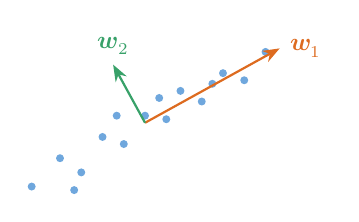
\begin{tikzpicture}[scale=0.9]
  \begin{scope}
    \foreach \x/\y in {-1.6/-0.9,-1.2/-0.5,-0.9/-0.7,-0.6/-0.2,-0.3/-0.3,0/0.1,0.3/0.05,0.5/0.45,0.8/0.3,1.1/0.7,1.4/0.6,1.7/1.0,-1.0/-0.95,0.2/0.35,-0.4/0.1,0.95/0.55}
      \fill[dataC!70] (\x,\y) circle (1.6pt);
    \draw[-{Stealth[length=6pt]}, thick, accentC] (0,0) -- (1.9,1.05) node[right] {\small $\vw_1$};
    \draw[-{Stealth[length=6pt]}, thick, accentD] (0,0) -- (-0.45,0.82) node[above] {\small $\vw_2$};
  \end{scope}
\end{tikzpicture}
\end{titlepage}

\tableofcontents
\newpage

% ==================================================================
\section*{Key Facts at a Glance}
\addcontentsline{toc}{section}{Key Facts at a Glance}
\markboth{Key Facts at a Glance}{}
% ==================================================================

A running list of the facts that do the most work. Each one has \emph{why} it is true and
\emph{so what} it buys you, with a pointer to the full treatment. Throughout, $X\in\R^{N\times d}$ is
\textbf{centered} (each column has mean zero, $\one\T X=\bm0\T$), so that $\Sig=\tfrac1N X\T X$. To avoid a name clash, the
singular values of $X$ are written $\sigma_j$ and collected in $S=\diag(\sigma_1,\dots)$, while
$\Sig$ always means the covariance.

\begin{keyfactbox}{Rows are samples, columns are features: reading $X_{i:}$, $\vx_i$ and $X_{:j}$}\label{kf:indexing}
\begin{center}
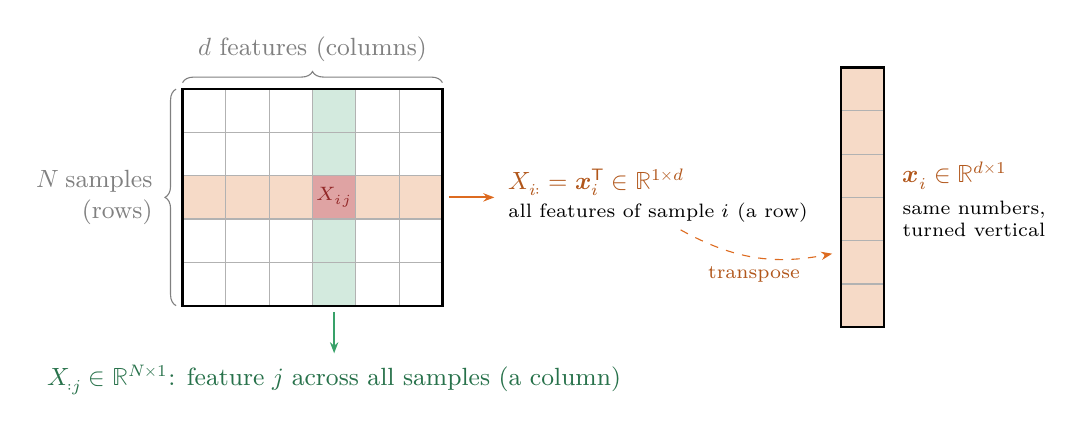
\begin{tikzpicture}[x=0.55cm,y=0.55cm, every node/.style={font=\small}]
  % column highlight (feature j = 4) and row highlight (sample i = 3)
  \fill[accentD!22] (3,0) rectangle (4,5);
  \fill[accentC!25] (0,2) rectangle (6,3);
  \fill[thmred!45] (3,2) rectangle (4,3);
  \draw[step=1, gray!60] (0,0) grid (6,5);
  \draw[thick] (0,0) rectangle (6,5);
  \node[thmred!80!black, font=\scriptsize] at (3.5,2.5) {$X_{ij}$};
  % axis labels
  \draw[decorate, decoration={brace, amplitude=4pt}, gray] (0,5.15) -- (6,5.15) node[midway, above=4pt] {$d$ features (columns)};
  \draw[decorate, decoration={brace, amplitude=4pt, mirror}, gray] (-0.15,5) -- (-0.15,0) node[midway, left=5pt, align=right] {$N$ samples\\(rows)};
  % row label
  \draw[accentC, thick, -{Stealth[length=4pt]}] (6.15,2.5) -- (7.2,2.5);
  \node[accentC!80!black, anchor=west] at (7.3,2.85) {$X_{i:}=\vx_i\T\in\R^{1\times d}$};
  \node[anchor=west, font=\scriptsize] at (7.3,2.15) {all features of sample $i$ (a row)};
  % the same row turned vertical
  \begin{scope}[shift={(15.2,-0.5)}]
    \fill[accentC!25] (0,0) rectangle (1,6);
    \draw[step=1, gray!60] (0,0) grid (1,6);
    \draw[thick] (0,0) rectangle (1,6);
    \node[accentC!80!black, anchor=west] at (1.2,3.5) {$\vx_i\in\R^{d\times1}$};
    \node[anchor=west, align=left, font=\scriptsize] at (1.2,2.5) {same numbers,\\turned vertical};
  \end{scope}
  \draw[accentC, dashed, -{Stealth[length=4pt]}] (11.5,1.75) to[bend right=20] node[below, font=\scriptsize, accentC!80!black] {transpose} (15.0,1.2);
  % column label
  \draw[accentD, thick, -{Stealth[length=4pt]}] (3.5,-0.15) -- (3.5,-1.1);
  \node[accentD!70!black, anchor=north] at (3.5,-1.15) {$X_{:j}\in\R^{N\times1}$: feature $j$ across all samples (a column)};
\end{tikzpicture}
\end{center}
\begin{itemize}[nosep]
\item $X_{i:}=\vx_i\T\in\R^{1\times d}$: all features of sample $i$ (row $i$ of $X$).
\item $\vx_i\in\R^{d\times1}$: those same features of sample $i$, turned vertical. Vectors are columns by default, which is why the row is written $\vx_i\T$.
\item $X_{:j}\in\R^{N\times1}$: feature $j$ measured on every sample (column $j$ of $X$).
\item $X_{ij}$: where they cross, feature $j$ of sample $i$.
\end{itemize}
\why The colon means ``all indices in this slot'': $X_{i:}$ fixes the row and runs over every column, and $X_{:j}$ fixes
the column and runs over every row. Stacking the rows gives $X=\begin{bmatrix}\vx_1\T\\\vdots\\\vx_N\T\end{bmatrix}$.
\sowhat Most formulas are a row or a column read out loud. A \textbf{row} operation acts on one sample:
the PC score $\vx_i\T\vw$ (row times loading), and $X\vw$ stacks those scores for all $N$ samples.
A \textbf{column} operation acts on one feature: its mean $\bar x_j=\tfrac1N\one\T X_{:j}$, its variance, and centering
($HX$ centers every column at once). $X\T X=\sum_i\vx_i\vx_i\T$ sums over samples (a $d\times d$ feature-by-feature matrix), while
$XX\T$ compares samples pairwise ($N\times N$, $(XX\T)_{ik}=\vx_i\T\vx_k$).
\end{keyfactbox}

\begin{keyfactbox}{Inner product $\langle\bm a,\bm b\rangle$ and length $\norm{\bm a}$}\label{kf:innerprod}
For real vectors $\bm a=(a_1,\dots,a_d)\T$ and $\bm b=(b_1,\dots,b_d)\T$, the \textbf{inner product} (dot product) and the \textbf{length} (norm) are
\[
\boxed{\langle\bm a,\bm b\rangle=a_1b_1+a_2b_2+\cdots+a_db_d=\bm a\T\bm b,}\qquad
\boxed{\norm{\bm a}=\sqrt{\langle\bm a,\bm a\rangle},\ \text{ i.e. }\ \norm{\bm a}^2=\langle\bm a,\bm a\rangle=\bm a\T\bm a .}
\]
$\langle\bm a,\bm b\rangle$ measures how \emph{aligned} two vectors are; $\norm{\bm a}$ measures the \emph{size} of one vector.
\why ``Aligned'' is exact: $\langle\bm a,\bm b\rangle=\norm{\bm a}\,\norm{\bm b}\cos\theta$, where $\theta$ is the angle between them. So the inner product is
positive when the vectors point roughly the same way, $0$ when they are perpendicular, and negative when they point apart.
Example: $\bm a=(3,4)$, $\bm b=(2,1)$ gives $\langle\bm a,\bm b\rangle=3\cdot2+4\cdot1=10$, $\norm{\bm a}^2=3^2+4^2=25$ so $\norm{\bm a}=5$, $\norm{\bm b}=\sqrt5$, and
$\cos\theta=\tfrac{10}{5\sqrt5}=\tfrac2{\sqrt5}\approx0.89$ (about $27^\circ$ apart).
\sowhat \textbf{Kernels are inner products of features:} $k(\vx,\bm z)=\langle\psi(\vx),\psi(\bm z)\rangle$, and with both inputs equal,
$k(\vx,\vx)=\langle\psi(\vx),\psi(\vx)\rangle=\norm{\psi(\vx)}^2$, the squared length of $\vx$'s feature vector. Expanding $\norm{\bm a-\bm b}^2=\langle\bm a-\bm b,\bm a-\bm b\rangle$ turns
lengths and distances into inner products:
\[
\norm{\bm a-\bm b}^2=\norm{\bm a}^2+\norm{\bm b}^2-2\langle\bm a,\bm b\rangle
\quad\Longrightarrow\quad
\norm{\psi(\vx)-\psi(\bm z)}^2=k(\vx,\vx)+k(\bm z,\bm z)-2k(\vx,\bm z) .
\]
So distances in feature space come from kernel values alone. This is the same identity as the MDS step
$D_{rs}^2=B_{rr}+B_{ss}-2B_{rs}$. For the RBF kernel, $k(\vx,\vx)=1$: every feature vector has length $1$, and the kernel value is just
the cosine of the angle between two of them.
\end{keyfactbox}

\begin{keyfactbox}{Reading set and map notation: $\times$, $(a,b)$, $\to$, $\mapsto$, $\smallsetminus$, $\{\cdot\mid\cdot\}$}\label{kf:notation}
{\renewcommand{\arraystretch}{1.35}
\small
\begin{xltabular}{\linewidth}{@{}>{\raggedright\arraybackslash}p{3.0cm}>{\raggedright\arraybackslash}p{4.3cm}>{\raggedright\arraybackslash}X@{}}
\toprule
notation & read it as & example \\
\midrule
\endhead
$A\times B$ & ``$A$ cross $B$'': all pairs $(a,b)$ with $a\in A$, $b\in B$ (Cartesian product) & $\R\times(0,2\pi)=\{(u,v):u\in\R,\ 0<v<2\pi\}$, an infinite horizontal strip of height $2\pi$ in $\R^2$ \\
$(a,b)$ vs.\ $[a,b]$ & open interval, endpoints \emph{excluded}; closed interval, endpoints \emph{included} & $(0,2\pi)$ leaves out $0$ and $2\pi$. (Context decides whether $(a,b)$ is an interval or a point of $\R^2$.) \\
$F:A\to B$ & ``$F$ maps $A$ into $B$''. $A$ is the \textbf{domain} (allowed inputs), $B$ the \textbf{codomain} (where outputs live) & $F:\R\times(0,2\pi)\to C$ takes a point of the strip and returns a point of the cylinder \\
$(u,v)\mapsto\cdots$ & ``sends $(u,v)$ to $\cdots$'': the rule for one input & $(u,v)\mapsto(\cos v,\ \sin v,\ u)$ is the same as writing $F(u,v)=\cdots$ \\
$\{\vx\in\R^2\mid\text{cond}\}$ & ``the set of $\vx$ in $\R^2$ \emph{such that} cond'' (set-builder; $|$ or $:$) & $S^1=\{(x,y)\in\R^2\mid x^2+y^2=1\}$, the unit circle \\
$A\smallsetminus B$ & ``$A$ minus $B$'': elements of $A$ not in $B$ & $S^1\smallsetminus\{(0,1)\}$ is the circle with its top point removed \\
$\subset,\ \subseteq,\ \in$ & is a subset of; is an element of & $C\subset\R^3$; $(0,1)\in S^1$ \\
$S^1,\ \R^d$ & unit circle (a 1-dimensional manifold); $d$-dimensional space & $S^2$ is the unit sphere in $\R^3$ \\
$F|_U$ & $F$ \emph{restricted} to the smaller domain $U$ & ``$\psi|_U$ is an isometry'' in the local-isometry definition \\
$g\circ f$,\ $f^{-1}$ & ``$g$ after $f$'' (apply $f$ first); the inverse map undoing $f$ & $\psi\circ g^{-1}$ in the non-uniqueness argument \\
$\inf$,\ $\argmin$ & greatest lower bound (a minimum that need not be attained); the input achieving the minimum & $d^M=\inf_\gamma(\text{length})$; $\widehat{\bm z}=\argmin_{\bm z}\rho(\bm z)$ \\
\bottomrule
\end{xltabular}}
\textbf{Words about maps.} $F:A\to B$ is \textbf{injective} (one-to-one) if different inputs give different outputs,
\textbf{surjective} (onto) if every point of $B$ is hit, and \textbf{bijective} if both, which is exactly when an inverse
$F^{-1}:B\to A$ exists. A set is \textbf{open} if it contains no boundary points: every point has a little ball around it inside
the set, like $(0,2\pi)$ but not $[0,2\pi]$. A map is \textbf{continuous} if nearby inputs give nearby outputs.
\why These are the words a manifold problem is written in: a chart is ``a continuous, invertible $\varphi:U\to\R^t$ on an open
$U$''. Reading the domain carefully often \emph{is} the problem, e.g.\ whether $0$ and $2\pi$ belong to it (Example~\ref{ex:cylhw}).
\sowhat Before solving, translate the statement into words: ``$F:\R\times(0,2\pi)\to C$, $F(u,v)=(\cos v,\sin v,u)$'' reads ``take the open
strip of height $2\pi$, use $v$ as an angle around the circle and $u$ as the height, and wrap the strip around the cylinder''.
\end{keyfactbox}

\begin{keyfactbox}{The centering matrix $H$ subtracts the mean from every row}\label{kf:centering}
$H=I_N-\tfrac1N\one\one\T$ is $N\times N$ and multiplies $X$ from the \emph{left}, so it acts on the $N$ rows
(observations). Split it into its two pieces:
\begin{itemize}[nosep]
\item $I_NX=X$: keep the data as is.
\item $\tfrac1N\one\one\T X=\one\big(\tfrac1N\one\T X\big)=\one\,\xbar\T$: a matrix whose \emph{every} row is the feature-mean vector $\xbar\T$.
\end{itemize}
\[
HX=X-\one\,\xbar\T,\qquad\text{so row $i$ of $HX$ is}\quad \vx_i\T-\xbar\T .
\]
\why Group the product as $\one(\one\T X)$. First, $\one\T X$ adds up the rows, giving the row of column
sums, and dividing by $N$ gives $\xbar\T$. Then $\one\,\xbar\T$ ($N\times1$ times $1\times d$) stacks that row $N$ times.
Example: $X=\begin{bmatrix}1&10\\2&20\\3&30\end{bmatrix}$ gives $\one\xbar\T=\begin{bmatrix}2&20\\2&20\\2&20\end{bmatrix}$ and
$HX=\begin{bmatrix}-1&-10\\0&0\\1&10\end{bmatrix}$.
\par\smallskip\textbf{``Centered'' in symbols.} $X$ is centered when every feature (column) has mean zero:
\[
\boxed{\one\T X=\bm0\T}\iff \xbar=\tfrac1NX\T\one=\bm0\iff HX=X\iff \textstyle\sum_{i=1}^N\vx_i=\bm0 .
\]
Here $\one\T X$ is the $1\times d$ row of column sums, so the condition says each column sums (equivalently, averages) to $0$.
Read row-wise, the $N$ data points sum to the zero vector. It does \emph{not} say each row's entries sum to $0$. Transposed,
$X\T\one=\bm0$ puts $\one$ in the null space of $X\T$, which is why centering caps the rank at $N-1$ (Fact~\ref{kf:rankcount}).
\par\smallskip\textbf{Shapes: inner vs.\ outer product of $\one$.}
\[
\underbrace{\one\T\one}_{(1\times N)(N\times1)}=\sum_{i=1}^N1\cdot1=N\ \ (\text{a scalar}),
\qquad
\underbrace{\one\one\T}_{(N\times1)(1\times N)}=\begin{bmatrix}1&\cdots&1\\\vdots&&\vdots\\1&\cdots&1\end{bmatrix}\ \ (N\times N).
\]
The scalar $\one\T\one=N$ is what makes the key identities work:
\[
H\one=\one-\tfrac1N\one(\one\T\one)=\one-\one=\bm0,\qquad
H^2=I-\tfrac2N\one\one\T+\tfrac1{N^2}\one(\one\T\one)\one\T=I-\tfrac2N\one\one\T+\tfrac1N\one\one\T=H .
\]
\sowhat Centering becomes ordinary matrix algebra. $H\one=\bm0$, $H\T=H$ and $H^2=H$ (Prop.~\ref{prop:Hprops})
give $\Sig=\tfrac1N(HX)\T(HX)=\tfrac1NX\T HX$ in one line. The side matters: $H$ on the \emph{left} subtracts
column means, $H$ on the \emph{right} subtracts row means, and $HAH$ does both. That double centering is
how MDS ($B=HAH$) and kernel PCA ($\widetilde K=HKH$) center points they can never see directly.
\end{keyfactbox}

\begin{keyfactbox}{The covariance formula: $\Sigma_Z=\tfrac1N Z\T HZ$, which is $\tfrac1NZ\T Z$ \emph{only} when $Z$ is centered}\label{kf:covformula}
For any data matrix $Z\in\R^{N\times d}$, centered or not,
\[
\boxed{\Sigma_Z=\frac1N Z\T HZ.}
\qquad\text{If $Z$ is centered, }HZ=Z\text{, so}\qquad \Sigma_Z=\frac1N Z\T HZ=\frac1N Z\T Z .
\]
\why The covariance is the average outer product of \emph{centered} rows, $\tfrac1N\sum_i(\bm z_i-\bar{\bm z})(\bm z_i-\bar{\bm z})\T=\tfrac1N(HZ)\T(HZ)$.
Since $H$ is symmetric and idempotent (Fact~\ref{kf:centering}), $(HZ)\T(HZ)=Z\T H\T HZ=Z\T H^2Z=Z\T HZ$, so
one $H$ in the middle does the work of both.
\sowhat \textbf{The trap:} for uncentered $Z$, the matrix $\tfrac1NZ\T Z$ is the \emph{second moment}, not the covariance:
\[
\tfrac1NZ\T Z=\Sigma_Z+\bar{\bm z}\,\bar{\bm z}\T ,
\]
the matrix version of $\mathbb E[z^2]=\operatorname{Var}(z)+(\mathbb Ez)^2$. Example: one feature with values $1,3$ gives
$\tfrac1NZ\T Z=\tfrac{1+9}2=5$, but $\Sigma_Z=1$ (deviations $\pm1$), and the gap is $\bar z^2=4$. \textbf{Transformed data}, $Z=XA$:
$HZ=(HX)A$, so $\Sigma_Z=\tfrac1NA\T X\T HXA=A\T\Sigma_XA$, the same rule as Cov$(A\vx)$ (Fact~\ref{kf:covA}) with the
data in rows.
\end{keyfactbox}

\begin{keyfactbox}{$X\T X$ and $XX\T$ are always symmetric and PSD}\label{kf:psd}
For \emph{any} real matrix $X$,
\[
(X\T X)\T=X\T X,\qquad (XX\T)\T=XX\T,\qquad
\bm v\T X\T X\bm v=\norm{X\bm v}^2\ge0,\qquad \bm u\T XX\T\bm u=\norm{X\T\bm u}^2\ge0 .
\]
\why Transposing a product reverses the order, and $(X\T)\T=X$, so $(X\T X)\T=X\T(X\T)\T=X\T X$. The
quadratic form is a squared length, which can never be negative (Prop.~\ref{prop:gram_psd}).
\sowhat Every covariance matrix ($\tfrac1NX\T X$), Gram matrix ($XX\T$, the MDS matrix $B$) and kernel
matrix ($K=\Phi\Phi\T$) inherits both properties for free.
\end{keyfactbox}

\begin{keyfactbox}{PSD does \emph{not} mean nonnegative entries}\label{kf:psdentries}
A PSD matrix can have negative entries off the diagonal. Only the diagonal is forced to be $\ge0$. For a covariance,
\[
\begin{aligned}
\Sigma_{ii}&=\operatorname{Var}(X_i)\ge0&&\text{always;}\\
\Sigma_{ij}&=\operatorname{Cov}(X_i,X_j)&&\text{any sign: negative when one tends to rise as the other falls.}
\end{aligned}
\]
Example: $X_2=-X_1$ with $\operatorname{Var}(X_1)=1$ gives $\Sigma=\begin{bmatrix}1&-1\\-1&1\end{bmatrix}$, which has negative entries but
eigenvalues $0$ and $2$, so it is PSD.
\why Expand the quadratic form and split it into diagonal and off-diagonal terms:
\[
\vx\T A\vx=\sum_{i,j}A_{ij}\,x_ix_j=\underbrace{\sum_iA_{ii}\,x_i^2}_{\text{squares: sign set by }A_{ii}}+\underbrace{2\sum_{i<j}A_{ij}\,x_ix_j}_{x_ix_j\text{ can be }\pm} .
\]
A diagonal entry always multiplies a square, so it must be $\ge0$ (take $\vx=\bm e_i$: $\bm e_i\T A\bm e_i=A_{ii}$). An off-diagonal
entry multiplies $x_ix_j$, which can be positive or negative, so a negative $A_{ij}$ is fine as long as the diagonal
terms outweigh it. \emph{Precisely}, for $A=\begin{bmatrix}a&c\\c&b\end{bmatrix}$, completing the square gives
\[
a x_1^2+2c\,x_1x_2+b x_2^2=a\Big(x_1+\tfrac ca x_2\Big)^2+\Big(b-\tfrac{c^2}{a}\Big)x_2^2\ \ge0\ \text{for all }\vx
\iff c^2\le ab .
\]
With $a=b=1$: $c=-\tfrac12$ is fine, $c=-1$ is exactly balanced, and $c=-2$ fails ($\vx=(1,1)$ gives $1+1-4=-2$).
For a covariance, $\vx=(1,1)$ reads $\operatorname{Var}(X_1+X_2)=\operatorname{Var}X_1+\operatorname{Var}X_2+2\operatorname{Cov}(X_1,X_2)$: a negative covariance subtracts,
but never enough to make a variance negative. In the example the negative entries are absorbed into a perfect square:
\[
\vx\T\Sigma\vx=x_1^2-2x_1x_2+x_2^2=(x_1-x_2)^2\ge0 .
\]
\sowhat Three consequences.
(i) PSD does limit the off-diagonal entries: every $2\times2$ principal minor is $\ge0$, so
$\Sigma_{ij}^2\le\Sigma_{ii}\Sigma_{jj}$, which is exactly $|\operatorname{corr}|\le1$.
(ii) The zero eigenvalue has eigenvector $\propto(1,1)$, and along it $\operatorname{Var}(X_1+X_2)=(1,1)\,\Sigma\,(1,1)\T=0$ because $X_1+X_2\equiv0$: a zero eigenvalue is a direction of
zero variance, i.e.\ an exact linear relation among the features (Section~3.3).
(iii) The converse fails too. Nonnegative entries do \emph{not} imply PSD: $\begin{bmatrix}0&1\\1&0\end{bmatrix}$ has eigenvalues $\pm1$.
``PSD'' (a property of the quadratic form) and ``nonnegative'' (a property of the entries, as in NMF) are
different conditions, and neither implies the other.
\end{keyfactbox}

\begin{keyfactbox}{When can a matrix be diagonalized?}\label{kf:diag}
A square $A\in\R^{n\times n}$ is \textbf{diagonalizable}, $A=PDP^{-1}$ with $D$ diagonal, exactly when it has enough eigenvectors:
\[
\boxed{\begin{aligned}
A\ \text{diagonalizable}&\iff A\ \text{has $n$ linearly independent eigenvectors}\\
&\iff \text{geometric mult.}=\text{algebraic mult.\ for every eigenvalue.}
\end{aligned}}
\]
Here the \emph{geometric} multiplicity of $\lambda$ is $\dim\ker(A-\lambda I)$ (the number of independent eigenvectors), and the
\emph{algebraic} multiplicity is how many times $\lambda$ is a root of $\det(A-\lambda I)$. A handy sufficient condition is that
$n$ \emph{distinct} eigenvalues always give $n$ independent eigenvectors.
\why In the standard axes $A$ may \emph{mix} coordinates, e.g.\ $(x,y)\mapsto(x+y,\,y)$. Diagonalizing means finding new axes
(the columns of $P$) along which $A$ does something very simple: $(z_1,\dots,z_n)\mapsto(\lambda_1z_1,\dots,\lambda_nz_n)$. Each
axis is stretched or flipped on its own, with no mixing. That needs $n$ independent directions that $A$ does not turn
away from themselves, which is the definition of eigenvectors.
\sowhat \textbf{It can fail.} The shear $A=\begin{bmatrix}1&1\\0&1\end{bmatrix}$ has eigenvalue $1$ twice (algebraic multiplicity
$2$), but $(A-I)\bm v=\begin{bmatrix}0&1\\0&0\end{bmatrix}\bm v=\bm0$ forces $\bm v=(a,0)\T$: only one independent eigenvector
(geometric multiplicity $1$). A shear slides every line parallel to the $x$-axis, so the only direction it leaves
alone is the $x$-axis itself. Also, even when $A$ \emph{is} diagonalizable, the axes need not be perpendicular:
$\begin{bmatrix}1&1\\0&2\end{bmatrix}$ has eigenvectors $(1,0)$ and $(1,1)$, which meet at $45^\circ$.
\end{keyfactbox}

\begin{keyfactbox}{Spectral theorem: symmetric $\Rightarrow$ diagonalizable by a \emph{rotation}}\label{kf:spectral}
\[
\boxed{A=A\T\ (\text{real})\ \Longrightarrow\ A=Q\Lambda Q\T,\quad Q\T Q=I,\quad \Lambda\ \text{real diagonal}.}
\]
The columns of $Q$ are \emph{orthonormal} eigenvectors (Thm.~\ref{thm:spectral}). The complex analogue needs
$A$ \textbf{Hermitian}, $A=A^*$ (conjugate transpose), and then $A=U\Lambda U^*$ with $U$ unitary.
\why Two short arguments carry the theorem. Eigenvalues are real: if $A\bm v=\lambda\bm v$ (possibly complex), compute $\bar{\bm v}\T A\bm v$ two ways. Directly it is
$\lambda\,\bar{\bm v}\T\bm v$. Using $A\T=A$ and $A$ real, it is $(A\bar{\bm v})\T\bm v=(\overline{A\bm v})\T\bm v=\bar\lambda\,\bar{\bm v}\T\bm v$. Since
$\bar{\bm v}\T\bm v=\sum_i|v_i|^2>0$, $\lambda=\bar\lambda$. Eigenvectors for different
eigenvalues are orthogonal: $\lambda_1\bm v_1\T\bm v_2=(A\bm v_1)\T\bm v_2=\bm v_1\T A\bm v_2=\lambda_2\bm v_1\T\bm v_2$, so
$(\lambda_1-\lambda_2)\bm v_1\T\bm v_2=0$. (That symmetric matrices also never run short of eigenvectors, as the shear did,
is the harder part of the proof.)
\sowhat Symmetry is the condition that buys \emph{perpendicular} axes and $Q^{-1}=Q\T$ for free. Every covariance,
Gram, MDS and kernel matrix in this course is symmetric (Fact~\ref{kf:psd}), so all of them get this clean
rotate--stretch--rotate-back form. If the matrix is also PSD, every $\lambda\ge0$.
\end{keyfactbox}

\begin{keyfactbox}{Every matrix has an SVD (any shape, diagonalizable or not)}\label{kf:svdexists}
\[
\boxed{\begin{gathered}
\text{Every real } A\in\R^{m\times n}\text{ factors as } A=USV\T,\\
U\T U=I_m,\quad V\T V=I_n,\quad S\ \text{diagonal } (m\times n)\ \text{with }\sigma_1\ge\sigma_2\ge\cdots\ge0.
\end{gathered}}
\]
\why Build it from the spectral theorem. $A\T A$ is symmetric PSD (Fact~\ref{kf:psd}), so $A\T A=V\Lambda V\T$ with
orthonormal $\bm v_i$ and $\lambda_i\ge0$. Set $\sigma_i=\sqrt{\lambda_i}$ and, for $\sigma_i>0$, $\bm u_i=A\bm v_i/\sigma_i$. These are
orthonormal automatically:
\[
\bm u_i\T\bm u_j=\frac{\bm v_i\T A\T A\bm v_j}{\sigma_i\sigma_j}=\frac{\sigma_j^2\,\bm v_i\T\bm v_j}{\sigma_i\sigma_j}=\begin{cases}1&i=j\\0&i\ne j\end{cases},
\]
and $A\bm v_i=\sigma_i\bm u_i$ is $AV=US$, i.e.\ $A=USV\T$. (Pad $U$ with extra orthonormal columns for the zero
$\sigma$'s.) Nothing here needed $A$ to be square, symmetric or diagonalizable.
\sowhat \textbf{The trick is to use two different sets of axes.} Eigen-decomposition demands the \emph{same} axes
going in and coming out, and that can fail. The SVD allows input axes $V$ and output axes $U$, and then
every matrix is just ``rotate, stretch each axis by $\sigma_i\ge0$, rotate''. Even the non-diagonalizable shear has one:
$\begin{bmatrix}1&1\\0&1\end{bmatrix}$ has $\sigma_1=\tfrac{1+\sqrt5}2\approx1.618$ and $\sigma_2=\tfrac{\sqrt5-1}2\approx0.618$ (eigenvalues of
$A\T A=\begin{bmatrix}1&1\\1&2\end{bmatrix}$ are $\tfrac{3\pm\sqrt5}2$). It stretches one direction by the golden ratio and shrinks the
perpendicular one by the same factor, so area is preserved ($\sigma_1\sigma_2=|\det A|=1$). For a symmetric
matrix the two decompositions agree up to signs: $\sigma_i=|\lambda_i|$, and for PSD matrices $\sigma_i=\lambda_i$.
\end{keyfactbox}

\begin{keyfactbox}{Linear-algebra toolbox: the other theorems that keep coming up}\label{kf:toolbox}
\begin{itemize}[leftmargin=1.3em]
\item \textbf{Rank--nullity.} For $A\in\R^{m\times n}$: $\rank A+\dim\ker A=n$. Every input direction is either kept
(counted by the rank) or killed (the null space). \emph{Used for}: $\rank(HX)\le N-1$, since $\one\in\ker((HX)\T)$.
\item \textbf{Rank of a product.} $\boxed{\rank(AB)\le\min\{\rank A,\rank B\}}$: a product can never have more independent
directions than either ingredient.
\emph{Why, one half each:} every column of $AB$ is $A$ times a column of $B$, so $\col(AB)\subseteq\col(A)$ and
$\rank(AB)\le\rank A$. Every row of $AB$ is a row of $A$ times $B$, a combination of the rows of $B$, so
$\rank(AB)\le\rank B$.
\emph{It can be strict:} $A=\begin{bmatrix}1&0\\0&0\end{bmatrix}$, $B=\begin{bmatrix}0&0\\0&1\end{bmatrix}$ both have rank $1$, but $AB=\bm0$ has rank $0$, because $B$ only
outputs the direction that $A$ kills. Same with $B'=\begin{bmatrix}0&0\\1&0\end{bmatrix}$: $AB'=\bm0$, yet $B'A=\begin{bmatrix}0&0\\1&0\end{bmatrix}$ has rank $1$, so the
\emph{order} of the product matters. The rule is only an upper bound, and the rank can fall anywhere from $0$ up to it.
\emph{Equality} holds when nothing is lost, e.g.\ if $A$ is invertible (or has independent columns), then $\rank(AB)=\rank B$.
That is why $\rank(USV\T)=\rank S$. ($\rank(A\T A)=\rank A$ is also an equality case, but for a different reason: see the next bullet.)
\emph{Used for}: $X=WH$ with $k$ parts $\Rightarrow\rank X\le k$ (NMF, nonnegative rank); $\rank(HX)\le\min\{\rank H,\rank X\}\le\min\{N-1,d\}$
(at most $N-1$ nonzero PC variances); and the Gram matrix $K=\Phi\Phi\T$ has rank at most the feature dimension.
\item \textbf{$\rank(A\T A)=\rank(A)$.} $A\T A\bm x=\bm0\Rightarrow\bm x\T A\T A\bm x=\norm{A\bm x}^2=0\Rightarrow A\bm x=\bm0$, so both have the same
null space. \emph{Used for}: the number of nonzero PC variances equals $\rank(HX)$.
\item \textbf{Trace and determinant from eigenvalues.} $\tr A=\sum_i\lambda_i$ and $\det A=\prod_i\lambda_i$ (counted with algebraic
multiplicity). \emph{Used for}: total variance $=\tr\Sig=\sum\lambda_j$, and the characteristic-polynomial shortcut
$\lambda^2-(\tr A)\lambda+\det A=0$ for $2\times2$ matrices.
\item \textbf{Invertible matrix theorem.} For square $A$, all of the following are equivalent: $A$ is invertible; $\det A\ne0$;
$0$ is not an eigenvalue; $\rank A=n$; $\ker A=\{\bm0\}$; the columns are independent; all $\sigma_i>0$. \emph{Used for}: $H$
is not invertible ($H\one=\bm0$), and a covariance with a zero $\lambda$ cannot be inverted (so Mahalanobis distance
needs $\lambda_j>0$).
\item \textbf{The four subspaces, read off the SVD.} With $r=\rank A$:
$\col A=\spn\{\bm u_1,\dots,\bm u_r\}$, $\ker A\T=\spn\{\bm u_{r+1},\dots\}$, $\operatorname{row}A=\spn\{\bm v_1,\dots,\bm v_r\}$ and
$\ker A=\spn\{\bm v_{r+1},\dots\}$. The row space is perpendicular to the null space, and the column space to $\ker A\T$.
\emph{Used for}: PCA's kept and discarded directions are orthogonal complements (Prop.~\ref{prop:keptdisc}).
\end{itemize}
\end{keyfactbox}

\begin{keyfactbox}{Rank is the width of the narrowest bottleneck}\label{kf:bottleneck}
Write a product with a thin middle dimension, e.g.\ $X=AZ\T$ with $A\in\R^{N\times3}$ and $Z\T\in\R^{3\times d}$, as a two-step map:
\[
\R^d\ \xrightarrow{\ Z\T\ }\ \R^{3}\ \xrightarrow{\ A\ }\ \R^N .
\]
However large $N$ and $d$ are, every vector must squeeze through the middle space $\R^3$, which has only three
independent ``channels''. So
\[
\boxed{\rank(AZ\T)\le3}\qquad\text{and in general}\qquad \rank(\underbrace{A}_{N\times k}\underbrace{B}_{k\times d})\le k .
\]
\textbf{When all channels survive.} The rank is \emph{exactly} $k$ if (i) $B$ has rank $k$, so it can reach every direction of the
middle $\R^k$ (it is onto), and (ii) $A$ has rank $k$, so it keeps those $k$ directions distinct instead of collapsing one
(independent columns). If either factor wastes a channel, the rank drops below $k$ (the strict examples in Fact~\ref{kf:toolbox}).
\why The output of $AB$ is $A$ applied to the outputs of $B$, which live in a $k$-dimensional space. A linear map
cannot turn a $k$-dimensional set of inputs into more than $k$ independent outputs (rank of a product, Fact~\ref{kf:toolbox}).
\sowhat \textbf{The converse is the useful part:} every rank-$k$ matrix \emph{is} such a bottleneck product. For example,
$X=(U_kS_k)\,V_k\T$ from the SVD, which is $(N\times k)(k\times d)$. So
\[
\rank X\le k\iff X=AB\ \text{for some }A\in\R^{N\times k},\ B\in\R^{k\times d}.
\]
Low-rank approximation is choosing the best $k$-channel bottleneck. PCA/SVD route the data through $k$ orthogonal
channels (scores $\times$ loadings), NMF through $k$ nonnegative ones ($W\times H$). In both, ``rank $k$'' means ``every sample is
described by $k$ numbers''. The nonnegative rank (Thm.~\ref{thm:nnsandwich}) is the narrowest bottleneck
when the channels must also be nonnegative.
\end{keyfactbox}

\begin{keyfactbox}{The covariance is diagonalizable by a rotation, with nonnegative eigenvalues}
Since $\Sig=\tfrac1NX\T X$ is symmetric, the spectral theorem (Thm.~\ref{thm:spectral}) applies:
\[
\Sig=V\Lambda V\T,\qquad V\T V=I,\qquad \Lambda=\diag(\lambda_1\ge\cdots\ge\lambda_d),\qquad \lambda_j\ge0 .
\]
\why Symmetric $\Rightarrow$ real eigenvalues and an orthonormal eigenbasis. PSD $\Rightarrow$ each
$\lambda_j=\bm v_j\T\Sig\bm v_j\ge0$.
\sowhat This is all of PCA. The columns $\bm v_j$ are perpendicular \emph{loadings} (new axes), and
$\lambda_j$ is the variance along axis $j$. Nonnegativity is what lets $\lambda_j$ \emph{be} a variance,
$\sqrt{\lambda_j}$ a standard deviation, and $\sum_{j\le k}\lambda_j/\sum_j\lambda_j$ a proportion
(Section~\ref{sec:pca}).
\end{keyfactbox}

\begin{keyfactbox}{$\operatorname{Cov}(A\vx+\bm b)=A\,\Sigma_x\,A\T$: the matrix version of $\operatorname{Var}(ax)=a^2\operatorname{Var}(x)$}\label{kf:covA}
For a random vector $\vx$ with mean $\bm\mu$ and known covariance $\Sigma_x=\operatorname{Cov}(\vx)$, and any constant $A$ ($m\times d$) and $\bm b$:
\[
\begin{aligned}
\text{scalar:}&\quad \operatorname{Var}(ax+b)=a\,\operatorname{Var}(x)\,a=a^2\operatorname{Var}(x),\\
\text{vector:}&\quad \operatorname{Cov}(A\vx+\bm b)=\underbrace{A}_{m\times d}\,\underbrace{\Sigma_x}_{d\times d}\,\underbrace{A\T}_{d\times m}\qquad(m\times m).
\end{aligned}
\]
\why Expand the definition. The shift cancels, $A\vx+\bm b-(A\bm\mu+\bm b)=A(\vx-\bm\mu)$, and transposing a
product reverses it, $\big(A(\vx-\bm\mu)\big)\T=(\vx-\bm\mu)\T A\T$. So
\[
\operatorname{Cov}(A\vx+\bm b)=\mathbb E\big[A(\vx-\bm\mu)(\vx-\bm\mu)\T A\T\big]=A\,\mathbb E\big[(\vx-\bm\mu)(\vx-\bm\mu)\T\big]A\T=A\Sigma_xA\T .
\]
The transpose is the matrix way to ``square'' $A$. $A^2$ need not even exist ($A$ may not be square), and
covariance compares the output with \emph{itself}: one copy of the deviation is transformed by $A$ on the left,
the other by $A\T$ on the right. (Prop.~\ref{prop:covaffine}.)
\sowhat Three special cases run the whole course:
\begin{itemize}[nosep]
\item $A=\vw\T$ ($1\times d$, a single direction): $\operatorname{Var}(\vw\T\vx)=\vw\T\Sigma_x\vw$, the quantity PCA maximizes over unit $\vw$ (Prop.~\ref{prop:rayleigh}).
\item $A=V\T$ (all the loadings): $\operatorname{Cov}(\text{scores})=V\T\Sigma_xV=\Lambda$. The PC scores are uncorrelated with variances $\lambda_j$ (Thm.~\ref{thm:scores}).
\item $A=D=\diag(c_1,\dots,c_d)$ (rescaling units): $D\Sigma_xD$, entry $(j,k)$ times $c_jc_k$. That is why PCA depends on units, and why standardizing gives the correlation matrix.
\end{itemize}
\end{keyfactbox}

\begin{keyfactbox}{Every observation = scores $\times$ feature directions}\label{kf:scoresdirs}
With the SVD $X=USV\T$ of the centered data (Fact~\ref{kf:svdcov}), row $i$ of $X$ reads
\[
\underbrace{\vx_i\T}_{1\times d}=\sum_{j=1}^{r}\underbrace{(\sigma_ju_{ij})}_{\text{score}}\ \underbrace{\vv_j\T}_{\text{direction}},
\qquad\text{i.e.}\qquad
\vx_i\T=\underbrace{(US)_{i:}}_{\text{scores}}\ \underbrace{V\T}_{\text{feature directions}} .
\]
\begin{itemize}[nosep]
\item $\vv_j$ (a loading) is the $j$th \textbf{new axis}, written as a recipe of the \emph{old} features: its entry $(\vv_j)_\ell$ says how much original feature $\ell$ goes into it.
\item $\sigma_ju_{ij}=\vx_i\T\vv_j$ is observation $i$'s \textbf{score}: its coordinate along that new axis.
\item Multiplying by $V\T$ translates the scores \emph{back} into the original feature coordinates.
\end{itemize}
Keeping only $k$ terms is PCA: $\;\vx_i\T\approx\sum_{j=1}^{k}(\sigma_ju_{ij})\,\vv_j\T$, the best rank-$k$ approximation (Fact~\ref{kf:trunc}).
\why $X=USV\T$ read row by row: row $i$ of $US$ times $V\T$. Since $V\T V=I$, multiplying both sides by $\vv_j$
picks out one coefficient, $\vx_i\T\vv_j=\sigma_ju_{ij}$ (``read off the coordinates'', Section~1.1).
\sowhat It is the same ``coefficients $\times$ patterns'' shape as NMF:
\[
\vx_i\T\approx\underbrace{W_{i:}}_{\text{nonnegative weights}}\ \underbrace{H}_{\text{nonnegative patterns}} .
\]
The difference is the constraints. PCA's directions are orthonormal and its scores have any sign. NMF's
patterns are nonnegative and can be added but never subtracted.
\end{keyfactbox}

\begin{intuition}
\textbf{Scores are not ``the new dimensions''. The rows of $V\T$ are.} With features (height, weight), a
first loading $\vv_1\approx(0.97,\ 0.24)$ defines the new axis ``$0.97\cdot$height $+\ 0.24\cdot$weight'', a blend of the
old axes. A person's PC1 score is \emph{where they sit} along that blend. Two details:
(1) loadings have \emph{unit length}, so a recipe like $(0.8,\ 0.2)$ must be rescaled by $1/\sqrt{0.8^2+0.2^2}$ to
$\approx(0.97,\ 0.24)$; (2) features in different units should be standardized first (Section~2.6), and a
category such as eye colour would need a numeric encoding before it can enter a recipe at all.
\textbf{Why the blend beats any single feature:} each original axis $\bm e_\ell$ is itself a unit direction, so
\[
\lambda_1=\max_{\norm{\vv}=1}\vv\T\Sig\vv\ \ge\ \bm e_\ell\T\Sig\bm e_\ell=\Sig_{\ell\ell}=\operatorname{Var}(\text{feature }\ell)\quad\text{for every }\ell .
\]
PC1 captures at least as much variance as the best single original feature, and strictly more whenever
features are correlated.
\end{intuition}

\begin{keyfactbox}{Total variance splits into kept + discarded}\label{kf:totalvar}
\[
\text{total variance}=\tr\Sig=\sum_{j=1}^d\lambda_j
=\underbrace{\sum_{j\le k}\lambda_j}_{\text{kept}}
+\underbrace{\sum_{j>k}\lambda_j}_{\text{discarded}} .
\]
The kept part is the variance captured by the first $k$ PCs; the discarded part is the average
reconstruction error.
\why $\tr\Sig=\tr(V\Lambda V\T)=\tr(\Lambda V\T V)=\tr\Lambda$ (cyclic trace). Rotating the axes cannot
change the total spread. The discarded part equals $\tfrac1N\sum_i\norm{\vx_i-\widehat{\vx}_i^{(k)}}^2$
(Thm.~\ref{thm:bestsub}), and no other $k$-dimensional subspace does better.
\sowhat The scree plot and ``percent variance explained'' are just this split read off for each $k$.
\end{keyfactbox}

\begin{keyfactbox}{Truncated SVD error = sum of the discarded $\sigma_j^2$}\label{kf:trunc}
Keep the first $k$ components of $X=USV\T$: $\;X_k=U_kS_kV_k\T$. Then
\[
\Fro{X-X_k}^2=\sum_{j>k}\sigma_j^2,
\]
and this is the smallest possible over \emph{all} matrices of rank $\le k$ (Eckart--Young, Thm.~\ref{thm:eckart}).
\why $X-X_k=\sum_{j>k}\sigma_j\vu_j\vv_j\T$, and the pieces $\vu_j\vv_j\T$ are orthonormal in the Frobenius
inner product, so squared norms just add (Pythagoras).
\sowhat It is the same statement as Fact~\ref{kf:totalvar} seen through the SVD: divide by $N$ (Fact~\ref{kf:svdcov}) and
$\tfrac1N\Fro{X-X_k}^2=\sum_{j>k}\lambda_j$.
\end{keyfactbox}

\begin{keyfactbox}{The SVD of $X$ \emph{is} the eigendecomposition of the covariance}\label{kf:svdcov}
\[
X=USV\T\quad\Longrightarrow\quad \Sig=\tfrac1NX\T X=\tfrac1NVS\T U\T USV\T=V\Big(\tfrac{S\T S}{N}\Big)V\T .
\]
So the loadings are the right singular vectors ($V$), the PC variances are $\lambda_j=\sigma_j^2/N$, and the
scores are $XV=US$.
\why $U\T U=I$ cancels the middle. What is left is $V\,(\text{diagonal})\,V\T$ with $V$ orthogonal,
which is exactly the form of an eigendecomposition. Eigendecompositions of symmetric matrices are
unique up to sign and ties, so this \emph{is} the PCA one (Section~\ref{sec:pcasvd}).
\sowhat You never need to form $\Sig$. One SVD of the centered data gives loadings, variances and
scores at once, and it is more stable numerically. It also explains the units: $\sigma_j$ measures
spread in the original units $\times\sqrt N$, and $\lambda_j=\sigma_j^2/N$ is a variance.
\end{keyfactbox}

\begin{keyfactbox}{$\sigma_j^2$ is total spread, $\lambda_j$ is average spread: $\ \sigma_j^2=N\lambda_j$}\label{kf:sigmalambda}
\[
\begin{aligned}
\sigma_j^2&=\sum_{i=1}^N\big(\vx_i\T\vv_j\big)^2&&=\text{total squared spread of all $N$ points along PC $j$},\\
\lambda_j&=\frac{\sigma_j^2}{N}&&=\text{average squared spread per point along PC $j$},
\end{aligned}
\qquad\text{so}\qquad
\boxed{\ \sigma_j^2=N\lambda_j\ }
\]
\why From $X\vv_j=\sigma_j\vu_j$ with $\norm{\vu_j}=1$: $\sigma_j^2=\norm{X\vv_j}^2=\sum_i(\vx_i\T\vv_j)^2$, the sum of the squared PC-$j$
scores. Because $X$ is centered, those scores have mean $0$ (Thm.~\ref{thm:scores}), so their average square
\emph{is} their variance. That is $\lambda_j$.
\sowhat Read the SVD in plain words. $\sigma_j$ is a \emph{size} that grows with the number of points
(doubling the data set by duplicating every row multiplies $\sigma_j^2$ by $2$), while $\lambda_j$ is a \emph{rate}
that does not. Example: PC-$j$ scores $(-2,\,0,\,2)$ give $\sigma_j^2=4+0+4=8$ and $\lambda_j=8/3$; the standard deviation
along PC $j$ is $\sqrt{\lambda_j}=\sigma_j/\sqrt N$. Ratios such as $\sigma_j^2/\sum_\ell\sigma_\ell^2=\lambda_j/\sum_\ell\lambda_\ell$ (variance
explained) are the same either way. (With the $N-1$ convention, $\lambda_j=\sigma_j^2/(N-1)$; only the divisor changes.)
\end{keyfactbox}

\begin{keyfactbox}{Rank $=$ number of nonzero singular values; $=$ number of nonzero PC variances \emph{only if centered}}\label{kf:rankcount}
For \emph{any} matrix, centered or not,
\[
\boxed{\rank(X)=\#\{j:\sigma_j>0\}.}
\]
For centered $X$ (so $X=HX$) this also equals the number of nonzero PC variances, because
$\lambda_j=\sigma_j^2/N$ and $\sigma_j\ne0\iff\lambda_j\ne0$ (Fact~\ref{kf:sigmalambda}). For uncentered $X$ it need not, since PCA
analyses $HX$, not $X$.
\why $X=USV\T$ with $U,V$ orthogonal (invertible), and multiplying by invertible matrices never changes rank. So
$\rank X=\rank S$, the number of nonzero diagonal entries. Each nonzero $\sigma_j$ is one direction $\vv_j$ that
survives ($X\vv_j=\sigma_j\vu_j\ne\bm0$), and each zero $\sigma_j$ is a direction squashed flat. PC variances are the singular
values of the \emph{centered} matrix, $\lambda_j=\sigma_j(HX)^2/N$, so they count $\rank(HX)$.
\sowhat \textbf{How much can centering lower the rank?} At most by one, since $X=HX+\one\xbar\T$ adds back a rank-$1$ matrix.
It drops \emph{exactly} when $\one\in\col(X)$, i.e.\ some combination of the features is the same constant for every
sample. (Reason: $\col(HX)=H\,\col(X)$, and $H$ kills only the direction $\one$.)
\begin{itemize}[nosep]
\item $X=\begin{bmatrix}1&0\\0&1\end{bmatrix}$: columns sum to $\one$, so $\rank X=2$ but $\rank HX=1$ (one nonzero PC variance; two points lie on a line).
\item $X=\begin{bmatrix}10&1\\10&2\\10&3\end{bmatrix}$: feature 1 is always $10$ (a shared baseline), and feature 2 varies. The columns
$(10,10,10)\T$ and $(1,2,3)\T$ are independent, so $\rank X=2$. Centering sends them to $(0,0,0)\T$ and $(-1,0,1)\T$, so
$\rank X_c=1$. The ``everyone is $10$'' direction disappears completely.
\item $X=\begin{bmatrix}1&0\\0&1\\1&1\end{bmatrix}$: $\one\notin\col(X)$, so the rank stays $2$.
\end{itemize}
\textbf{Slogan: centering removes independent-but-non-varying column directions.} The precise version is that the
removed direction can be any \emph{combination} of columns that is constant across samples, not only a literal constant
column. In the first example neither column is constant, but their sum is $(1,1)\T$. There is at most one such
direction: any combination that is constant across samples equals $c\,\one$ for some $c$, so all of them point along
the single direction $\one$ in the column space. That is the ``drops by at most one'' fact again.
\par\smallskip
Exam pattern: ``rank $=$ \# nonzero $\sigma$'' always holds. ``Rank $=$ \# nonzero PC variances'' holds for centered $X$, and for
uncentered $X$ only when $\one\notin\col X$. ``Rank $=\min(N,d)$'' is only an upper bound, never guaranteed. For centered data
it is not even attainable when $N\le d$, since then $\rank\le N-1$.
\end{keyfactbox}

\begin{keyfactbox}{A lower-dimensional flat has probability zero}\label{kf:measurezero}
A plane feels large because it is infinite, but it is infinitely \emph{thin} in the surrounding space. Picture a
sheet of paper floating in a room: infinite area, zero thickness. Pick a point uniformly in the room and the
chance it lands \emph{exactly} on the paper is $0$. Formally, for a random vector $\bm v\in\R^d$ with a density
(e.g.\ Gaussian with $\Sigma\succ0$) and any affine subspace $F$ of dimension $<d$,
\[
\boxed{\Pr(\bm v\in F)=0.}
\]
\why Start with the plane $z=0$ in $\R^3$ and $\bm v=(V_1,V_2,V_3)$ i.i.d.\ $N(0,1)$. Landing on it means $V_3=0$, and a continuous
variable hits any single value with probability $0$. Any other flat lies inside some hyperplane $\{\vw\T\bm v=c\}$
(with $\vw\ne\bm0$), and $\vw\T\bm v$ is again a continuous variable: Gaussian with variance $\vw\T\Sigma\vw>0$ (Fact~\ref{kf:covA}). So
$\Pr(\vw\T\bm v=c)=0$. A rotation can always turn the flat into ``some coordinates $=$ constants''.
\sowhat Three consequences for PCA:
\begin{itemize}[nosep]
\item \textbf{Random data hit the rank bound exactly.} With i.i.d.\ continuous data, the centered rank is
$\min(N-1,d)$ with probability $1$. Each new point leaves the flat spanned by the earlier ones, so no
``accidental'' extra zero appears. Example: $50$ Gaussian points in $\R^{100}$ give exactly $49$ nonzero PC variances.
\item \textbf{An exact zero PC variance is a real signal.} Pure noise never produces one, so $\lambda_j=0$ (or $\one\in\col X$, Fact~\ref{kf:rankcount})
points to a genuine linear relation: a constant column, a feature that is a sum of others, and so on.
\item \textbf{Small-$N$ flats do not generalize.} When $N\le d$, the training points always fit on an $(N-1)$-dimensional flat,
so ``dimension reduction'' looks guaranteed. A fresh sample lands on that flat with probability $0$. The low
dimension is an artifact of having few points, not structure in the data.
\end{itemize}
\end{keyfactbox}

\begin{keyfactbox}{A kernel is valid only if it is symmetric positive definite}\label{kf:validkernel}
The kernel trick replaces $\langle\varphi(\vx),\varphi(\vy)\rangle$ with a cheap formula $k(\vx,\vy)$. Expanding by hand shows how:
$\varphi(x)=(x,x+1,x+2)$ gives $k(x,y)=xy+(x+1)(y+1)+(x+2)(y+2)=3xy+3x+3y+5$, with no 3-vector ever built (Example~\ref{ex:affinekernel}).
\why The RKHS theorem (Theorem~\ref{thm:rkhs}): if $k$ is symmetric and every kernel matrix is PSD, there is a unique Hilbert space of
functions in which $k$ is the inner product. Without that, no feature space stands behind the numbers.
\sowhat You cannot use any similarity function willy-nilly. Kernels built from a feature map (polynomial, RBF, and sums and products of
kernels) are safe; $\norm{\vx-\vy}^2$ is not, and an invalid $k$ gives kernel PCA negative ``variances''. An infinite feature map also
needs shrinking coordinates, or the inner product diverges.
\end{keyfactbox}

\newpage

% ==================================================================
\section*{Notation used throughout}
\addcontentsline{toc}{section}{Notation used throughout}
% ==================================================================

\begin{center}
\renewcommand{\arraystretch}{1.25}
\begin{tabular}{>{$}l<{$} p{0.68\linewidth}}
\toprule
\text{Symbol} & Meaning \\
\midrule
N & number of observations (samples, rows) \\
d & number of variables (features, columns) \\
\vx_1,\dots,\vx_N\in\R^d & the data points \\
X\in\R^{N\times d} & data matrix; row $i$ is $\vx_i\T$ \\
\xbar=\tfrac1N\sum_i\vx_i & sample mean \\
\one\in\R^N & the all-ones vector \\
H = I-\tfrac1N\one\one\T & the \emph{centering matrix} \\
\Sig & sample covariance matrix \\
W=[\vw_1\,\cdots\,\vw_d] & PCA loadings (orthonormal eigenvectors of $\Sig$) \\
\lambda_1\ge\cdots\ge\lambda_d\ge0 & PC variances (eigenvalues of $\Sig$) \\
Y=HXW & PCA scores; row $i$ is $\vy_i\T$, entry $y_{ij}=\vw_j\T(\vx_i-\xbar)$ \\
A=USV\T & singular value decomposition \\
\had,\ \hdiv & entrywise (Hadamard) product and division \\
\bottomrule
\end{tabular}
\end{center}

A vector is a \emph{column} vector unless it is transposed. So a data point is
$\vx_i\in\R^{d}$ (a column), and it sits in $X$ as the \emph{row} $\vx_i\T$.

\begin{careful}
\textbf{Transposing keeps the order.} If $V=[\,\vv_1\ \vv_2\ \cdots\ \vv_k\,]$ has columns $\vv_1,\dots,\vv_k$, then
\[
V\T=\begin{bmatrix}\ \vv_1\T\ \\[4pt] \ \vv_2\T\ \\[2pt] \vdots\\[2pt] \ \vv_k\T\ \end{bmatrix}:
\]
column $j$ becomes row $j$. The first column becomes the first row, and nothing is reversed. (Entrywise,
$(V\T)_{ji}=V_{ij}$.) This is why the rows of $V\T$ in the SVD $X=U\Sigma V\T$ are the loadings
$\vv_1\T,\vv_2\T,\dots$ in order. Do not confuse this with transposing a \emph{product}, where the factors
\emph{do} swap: $(BC)\T=C\T B\T$. One matrix keeps its order, and a product reverses.
\end{careful}

% ==================================================================
\section{Linear-Algebra Warm-up (Problem Set 1)}
% ==================================================================

Everything later rests on a few facts: orthogonality, orthonormal bases,
eigendecompositions of symmetric matrices, and the two matrix products $X\T X$ and
$XX\T$. Problem Set~1 practised exactly these, so we start there.

\subsection{Orthogonality and orthonormal bases}

\begin{definition}{Orthogonal, orthonormal}{orth}
Two vectors $\vu,\vv$ are \textbf{orthogonal} when $\vu\T\vv=0$. A list
$\vq_1,\dots,\vq_k$ is \textbf{orthonormal} if $\vq_i\T\vq_j=0$ for $i\ne j$ and
$\norm{\vq_i}=1$. Stacking them as columns of $Q$ gives $Q\T Q=I_k$. When $k$ equals
the dimension, $Q$ is an \textbf{orthogonal matrix} and $Q^{-1}=Q\T$.
\end{definition}

\begin{example}{Checking independence and building an orthonormal basis}{gs}
Let $\vw_1=(1,1,0,0)\T$, $\vw_2=(0,0,1,1)\T$, $\vw_3=(1,0,1,1)\T$ in $\R^4$.

\textbf{(a) Linear independence.} Put the vectors in as columns and row-reduce:
\[
\begin{bmatrix}1&0&1\\1&0&0\\0&1&1\\0&1&1\end{bmatrix}
\xrightarrow{r_2\leftarrow r_1-r_2}
\begin{bmatrix}1&0&1\\0&0&1\\0&1&1\\0&1&1\end{bmatrix}
\xrightarrow{\text{reorder, } r_4-r_3}
\begin{bmatrix}1&0&1\\0&1&1\\0&0&1\\0&0&0\end{bmatrix}.
\]
There are three pivots, so the rank is $3$ and the vectors are linearly independent.

\textbf{(b) Gram--Schmidt.} Here $\vw_1\perp\vw_2$ already, so we only normalise them:
$\vq_1=\tfrac1{\sqrt2}(1,1,0,0)\T$ and $\vq_2=\tfrac1{\sqrt2}(0,0,1,1)\T$. Then we take
out of $\vw_3$ its components along $\vq_1$ and $\vq_2$:
\[
\vw_3-(\vw_3\T\vq_1)\vq_1-(\vw_3\T\vq_2)\vq_2
=(1,0,1,1)-\tfrac12(1,1,0,0)-(0,0,1,1)=\left(\tfrac12,-\tfrac12,0,0\right),
\]
so $\vq_3=\tfrac1{\sqrt2}(1,-1,0,0)\T$.

\textbf{(c) Orthogonal complement.} A vector $\vx=(a,b,c,d)$ orthogonal to all three
must satisfy $a+b=0$, $c+d=0$ and $a+c+d=0$. These force $a=b=0$ and $c=-d$, so
the complement is spanned by $\tfrac1{\sqrt2}(0,0,1,-1)\T$.
\end{example}

\begin{careful}
In my handwritten scratch work I subtracted $(1,1,0,0)$ itself rather than its
projection $\tfrac12(1,1,0,0)$ and got $(0,-1,0,0)$, which is \emph{not} orthogonal to
$\vw_1$. The projection coefficient is $\vw_3\T\vq_1=1/\sqrt2$, and it multiplies the
\emph{unit} vector $\vq_1$. A quick check: every Gram--Schmidt output must have zero
dot product with every earlier $\vq$.
\end{careful}

\begin{intuition}
Projecting onto an orthonormal set is just ``read off the coordinates'':
$\proj(\vx)=(\vx\T\vq_1)\vq_1+(\vx\T\vq_2)\vq_2+\cdots$. PCA does exactly this with a
basis $\vw_1,\dots,\vw_d$ that it \emph{learns} from the data.
\end{intuition}

\subsection{The spectral theorem in action}

\begin{theorem}{Spectral theorem}{spectral}
Every real symmetric $A\in\R^{d\times d}$ can be written
$A=Q\Lambda Q\T$ with $Q$ orthogonal and $\Lambda=\diag(\lambda_1,\dots,\lambda_d)$ real.
The columns of $Q$ are orthonormal eigenvectors: $A\vq_j=\lambda_j\vq_j$.
\end{theorem}

\begin{example}{A $3\times3$ eigendecomposition}{eig3}
Take $A=\begin{bmatrix}2&1&1\\1&2&1\\1&1&2\end{bmatrix}=I+\one\one\T$. Expanding along the first row:
\[
\det(A-\lambda I)=(2-\lambda)\big[(2-\lambda)^2-1\big]-1\big[(2-\lambda)-1\big]+1\big[1-(2-\lambda)\big]
=(4-\lambda)(1-\lambda)^2 .
\]
\begin{itemize}[nosep]
\item $\lambda=4$: solve $(A-4I)\vv=0$, which gives $\vv\propto(1,1,1)\T$.
\item $\lambda=1$ (twice): $(A-I)\vv=\one\one\T\vv=0$, i.e.\ every $\vv$ with $v_1+v_2+v_3=0$.
This is a whole 2-dimensional eigenspace (the plane $\perp\one$).
\end{itemize}
\end{example}

\begin{intuition}
$A=I+\one\one\T$ adds ``$3\times$ the mean'' in the $\one$ direction and leaves every
direction orthogonal to $\one$ alone. Reading eigenvectors off the structure like this
is often faster than computing the determinant.
\end{intuition}

\begin{proposition}{Inverse via the eigendecomposition}{inv}
If $A=Q\Lambda Q\T$ is invertible, then
$A^{-1}=(Q\T)^{-1}\Lambda^{-1}Q^{-1}=Q\Lambda^{-1}Q\T$.
For the example above this gives $A^{-1}=I-\tfrac14\one\one\T$.
\end{proposition}

\begin{careful}
The order flips when you invert a product: $(BC)^{-1}=C^{-1}B^{-1}$, just as
$(BC)\T=C\T B\T$. My first attempt wrote $Q^{-1}\Lambda^{-1}Q$, which is wrong.
The fix is $(Q\T)^{-1}=Q$.
\end{careful}

\subsection{Positive semidefinite matrices}

\begin{definition}{Positive semidefinite (PSD)}{psd}
A symmetric $A\in\R^{n\times n}$ is \textbf{positive semidefinite}, written $A\succeq0$, if
$\vx\T A\vx\ge0$ for every $\vx\in\R^n$.
\end{definition}

\begin{proposition}{Eigenvalue test}{psdeig}
A symmetric matrix is PSD if and only if every eigenvalue is $\ge0$. One negative eigenvalue is enough to fail.
\end{proposition}
\begin{proofsketch}
With $A=Q\Lambda Q\T$ and $\vy=Q\T\vx$, we have $\vx\T A\vx=\sum_j\lambda_jy_j^2$ (as in Prop.~\ref{prop:rayleigh}). If all
$\lambda_j\ge0$, this is a sum of nonnegative terms. If $\lambda_j<0$, take $\vx=\vq_j$: then $\vx\T A\vx=\lambda_j<0$.
\end{proofsketch}

\begin{proposition}{Every Gram matrix is PSD}{gram_psd}
For any real $A\in\R^{m\times n}$, the matrix $A\T A$ is PSD (and so is $AA\T$).
\end{proposition}
\begin{proofsketch}
Fix $\vx$ and let $\vy=A\vx$. Then $\vx\T A\T A\vx=(A\vx)\T(A\vx)=\vy\T\vy=y_1^2+\cdots+y_m^2\ge0$.
\end{proofsketch}

\begin{intuition}
$\vx\T A\T A\vx$ is not just \emph{like} a sum of squares. It \emph{is} one: the squared length of
the vector $A\vx$. So ``nonnegative for every $\vx$'' is no surprise. This one fact gives
PSD-ness of covariance matrices ($\tfrac1N(HX)\T(HX)$), of the classical-scaling matrix $B=XX\T$, and of
kernel matrices built from features ($K=\Phi\Phi\T$). It is also why the converse questions are
interesting: when is a given symmetric matrix of this form? For distance matrices the answer
is Theorem~\ref{thm:edm}, and for kernels it is Mercer's condition.
\end{intuition}

\subsection{The trace}

\begin{definition}{Trace}{trace}
The \textbf{trace} of a square matrix is the sum of its diagonal entries:
$\tr(A)=\sum_{i}A_{ii}$. For example $\tr\begin{bmatrix}2&7\\1&5\end{bmatrix}=2+5=7$.
\end{definition}

\begin{proposition}{The three facts we use}{traceprops}
\begin{enumerate}[nosep,label=(\roman*)]
\item \textbf{Cyclic:} $\tr(PQ)=\tr(QP)$ whenever both products are square, even if $P$ and $Q$ are not. Hence $\tr(PQR)=\tr(RPQ)=\tr(QRP)$.
\item \textbf{Sum of eigenvalues:} for symmetric $A=Q\Lambda Q\T$, $\tr(A)=\tr(\Lambda Q\T Q)=\tr(\Lambda)=\sum_j\lambda_j$.
\item \textbf{Sum of squares:} $\tr(X\T X)=\sum_{i,j}X_{ij}^2=\Fro{X}^2$, because $(X\T X)_{jj}$ is the squared length of column $j$.
\end{enumerate}
\end{proposition}
\begin{proofsketch}
(i) $\tr(PQ)=\sum_i\sum_kP_{ik}Q_{ki}=\sum_k\sum_iQ_{ki}P_{ik}=\tr(QP)$. The double sum is the same,
only the order of summation changes. (ii) and (iii) follow from (i) and the definition.
\end{proofsketch}

\begin{intuition}
Why statisticians care: applied to a covariance matrix, (iii) says
$\tr(\Sig)=\sum_j\operatorname{Var}(\text{feature }j)$, the \textbf{total variance}, and (ii) says
it also equals $\sum_j\lambda_j$. A rotation changes the eigenvectors but not the eigenvalues,
so it cannot change the total variance. Almost every ``variance is preserved'' or ``error equals
the sum of the discarded $\lambda$'s'' statement in these notes is a trace argument.
\end{intuition}

\subsection{Quadratic forms and the Rayleigh quotient}

\begin{proposition}{Extremes of a quadratic form}{rayleigh}
Let $A=Q\Lambda Q\T$ be symmetric with $\lambda_1\ge\cdots\ge\lambda_d$. Then
\[
\max_{\norm{\vx}=1}\vx\T A\vx=\lambda_1, \qquad \min_{\norm{\vx}=1}\vx\T A\vx=\lambda_d,
\]
attained at the corresponding eigenvectors.
\end{proposition}
\begin{proofsketch}
Write $\vy=Q\T\vx$. Since $Q$ is orthogonal, $\norm{\vy}=\norm{\vx}=1$, and
$\vx\T A\vx=(\vx\T Q)\Lambda(Q\T\vx)=\sum_j\lambda_j y_j^2$. This is a weighted
average of the $\lambda_j$ with weights $y_j^2$ that sum to $1$, so it lies between
$\lambda_d$ and $\lambda_1$. For the example: $\vx\T A\vx=4y_1^2+y_2^2+y_3^2\in[1,4]$.
\end{proofsketch}

\begin{deeper}
This one fact \emph{is} PCA. The variance of the data projected on a unit direction
$\vw$ is $\vw\T\Sig\vw$, a quadratic form. The direction of greatest variance is
therefore the top eigenvector of $\Sig$ (Section~\ref{sec:pca}).
\end{deeper}

\subsection{The two Gram products $X\T X$ and $XX\T$}\label{sec:gram}

With $X\in\R^{N\times d}$ having rows $\vx_i\T$:
\[
\underbrace{X\T X}_{d\times d}=\sum_{i=1}^N \vx_i\vx_i\T \quad(\text{sum of outer products}),\qquad
\underbrace{XX\T}_{N\times N}=\big[\vx_i\T\vx_j\big]_{i,j}\quad(\text{all pairwise inner products}).
\]
Shapes check: $(d\times N)(N\times d)$ is $d\times d$, and $(N\times d)(d\times N)$ is $N\times N$.
A function such as $f(\vx_1,\dots,\vx_N)=\sum_{i,j}(\vx_i\T\vx_j)^2$ is just
$\Fro{XX\T}^2$.

\begin{deeper}
$\Fro{XX\T}^2=\Fro{X\T X}^2=\sum_k\sigma_k^4$, where the $\sigma_k$ are the singular
values of $X$ (Section~\ref{sec:svd}). The $d\times d$ matrix $X\T X$ is the
covariance view that PCA uses. The $N\times N$ matrix $XX\T$ is the Gram view that
MDS and kernel PCA use. They share their nonzero eigenvalues, and that shared
spectrum is why PCA can be computed ``three ways'' (Section~\ref{sec:threeways}).
\end{deeper}

\subsection{Calculus reminders from the problem set}

\begin{example}{Unit tangent of a space curve}{tangent}
Let $\bm r(t)=(\cos t+t\sin t,\ \sin t-t\cos t,\ t^2)$. Then
\[
\bm r'(t)=(-\sin t+\sin t+t\cos t,\ \cos t-\cos t+t\sin t,\ 2t)=(t\cos t,\ t\sin t,\ 2t),
\]
so $\norm{\bm r'(t)}=t\sqrt5$ for $t>0$. The unit tangent is
$\bm T(t)=\tfrac1{\sqrt5}(\cos t,\sin t,2)$ and
$\bm T'(t)=\tfrac1{\sqrt5}(-\sin t,\cos t,0)$. At $t=2$:
$\bm r'(2)=(2\cos2,2\sin2,4)$ with length $2\sqrt5$.
\end{example}

\begin{example}{Gradient and linear approximation}{grad}
For $f(x,y)=x^2y+\sin(xy)+e^{x+y}$,
\[
\nabla f=\begin{bmatrix}2xy+y\cos(xy)+e^{x+y}\\ x^2+x\cos(xy)+e^{x+y}\end{bmatrix},
\qquad \nabla f(0,0)=\begin{bmatrix}1\\1\end{bmatrix}.
\]
The linear approximation at the origin is
$L(x,y)=f(0,0)+\nabla f(0,0)\T\begin{bmatrix}x\\y\end{bmatrix}=1+x+y$.
\end{example}

\begin{careful}
Don't forget the constant term $f(0,0)=e^0=1$. The notes wrote ``$+(0,0)$'' where
the base value belongs.
\end{careful}

% ==================================================================
\section{Principal Component Analysis}\label{sec:pca}
% ==================================================================

\subsection{Setup: centering and the covariance matrix}

We have data $\vx_1,\dots,\vx_N\in\R^d$. \textbf{Always center the data before
computing principal components:} $\vx_i\mapsto\vx_i-\xbar$. In matrix form, centering
is multiplication by the centering matrix.

\begin{definition}{Centering matrix}{H}
\[
H=I_N-\frac1N\one\one\T=
\begin{bmatrix}1&&\\&\ddots&\\&&1\end{bmatrix}-\frac1N\begin{bmatrix}1&\cdots&1\\\vdots&&\vdots\\1&\cdots&1\end{bmatrix}.
\]
$HX$ is the centered data matrix: row $i$ of $HX$ is $(\vx_i-\xbar)\T$.
\end{definition}

\begin{proposition}{Properties of $H$}{Hprops}
\begin{enumerate}[nosep,label=(\roman*)]
\item $H\one=\one-\tfrac1N\one(\one\T\one)=\one-\one=\bm 0$. Centering a constant gives zero.
\item $H\T=H$ (symmetric) and $H^2=H$ (idempotent). Centering twice changes nothing.
\item $H$ is the orthogonal projection onto $\{\bm v:\one\T\bm v=0\}$, so $\rank H=N-1$.
\item $\one\T(HX)=(H\one)\T X=\bm 0\T$. Every column of the centered matrix sums to zero.
\end{enumerate}
\end{proposition}

\begin{example}{Centering by hand}{centerex}
Take $N=3$ observations of $d=2$ features,
$X=\begin{bmatrix}1&10\\2&20\\3&30\end{bmatrix}$. The feature means are
$\xbar=(2,20)\T$. Subtracting $\xbar\T$ from every row gives
\[
X_c=HX=X-\one\xbar\T=\begin{bmatrix}-1&-10\\0&0\\1&10\end{bmatrix},
\qquad
\one\T X_c=\big[\,{-1}+0+1,\ \ {-10}+0+10\,\big]=[\,0\ \ 0\,].
\]
Why the centered column always sums to zero: if a column holds $x_1,\dots,x_N$ with mean
$\mu=\tfrac1N\sum_ix_i$, then $\sum_i(x_i-\mu)=\sum_ix_i-N\mu=0$, because $N\mu=\sum_ix_i$ by definition.
Multiplying by $\one\T$ adds up the rows, so $\one\T X_c=\bm0\T$ says exactly that
each feature column has mean zero.
\end{example}

\begin{intuition}
\textbf{What centering does and does not change.} Centering slides the whole cloud so
its mean sits at the origin. It does \emph{not} change any variance, because variance
is already measured around the mean: $\operatorname{Var}(x)=\tfrac1N\sum_i(x_i-\bar x)^2$
is the same before and after subtracting $\bar x$. For example, $\{2,3,4\}$ and
$\{-1,0,1\}$ both have variance $\tfrac23$. What centering removes is the
\emph{location} of the cloud. Without it, PCA measures spread around the origin
instead of around the mean, and a large mean offset can masquerade as the
``direction of greatest variance''. The first loading then just points at $\xbar$.
\end{intuition}

\begin{definition}{Sample covariance}{cov}
\[
\Sig=\Sig_X=\frac1N(HX)\T(HX)=\frac1N X\T H X=\frac1N\sum_{i=1}^N(\vx_i-\xbar)(\vx_i-\xbar)\T.
\]
When $X$ is already centered this is simply $\Sig=\tfrac1N X\T X$.
\end{definition}

\begin{careful}
Some texts divide by $N-1$ instead of $N$. Every eigenvalue scales by the same factor,
so the loadings, the ordering, and the proportions of variance are unchanged. Only the
reported variances differ slightly.
\end{careful}

\begin{example}{Computing a covariance matrix by hand, and what dividing by $N$ does}{covbyhand}
Three people, two features: $\vx_1=(1,2)$, $\vx_2=(2,3)$, $\vx_3=(3,1)$.
\begin{enumerate}[nosep,label=\arabic*.]
\item \textbf{Mean of each feature:} $\xbar=\big(\tfrac{1+2+3}3,\tfrac{2+3+1}3\big)=(2,2)$.
\item \textbf{Center} (subtract $\xbar$ from every row): each row now says how far that person is from average,
\[
X_c=\begin{bmatrix}-1&0\\0&1\\1&-1\end{bmatrix}.
\]
\item \textbf{Total spread} $S=X_c\T X_c=\sum_i(\vx_i-\xbar)(\vx_i-\xbar)\T$:
\[
S=\begin{bmatrix}-1&0&1\\0&1&-1\end{bmatrix}\begin{bmatrix}-1&0\\0&1\\1&-1\end{bmatrix}=\begin{bmatrix}2&-1\\-1&2\end{bmatrix}.
\]
The diagonal $2$'s are each feature's total squared deviation, e.g.\ $(-1)^2+0^2+1^2=2$. The $-1$ says the features tend to move
in opposite directions.
\item \textbf{Average it:} $\Sig=\tfrac1NS=\tfrac13S=\begin{bmatrix}2/3&-1/3\\-1/3&2/3\end{bmatrix}$. Feature 1's variance is $\tfrac{1+0+1}3=\tfrac23$.
\end{enumerate}
\textbf{Loadings and variances.} $S$ has eigenvectors $\vv_1=\tfrac1{\sqrt2}(1,-1)$ (eigenvalue $3$) and $\vv_2=\tfrac1{\sqrt2}(1,1)$
(eigenvalue $1$), so the PC variances are $\lambda_1=3/3=1$ and $\lambda_2=1/3$. PC1 $=\tfrac1{\sqrt2}(\text{feature 1})-\tfrac1{\sqrt2}(\text{feature 2})$
(centered values), a ``feature 1 high while feature 2 low'' direction. The signs can be flipped, since $\vv$ and $-\vv$ are the same axis.
A loading is the recipe for combining the original features into a PC. The eigenvalue $\lambda_j=\vv_j\T\Sig\vv_j$ is the
\emph{variance of the data along that direction}, the average squared score, not the length of the eigenvector (which is $1$).

\textbf{Dividing by $N$ changes sizes, never directions.} Add the mean itself as a 4th person, $\vx_4=\xbar=(2,2)$. The mean
stays $(2,2)$, the new centered row is $(0,0)$, and it adds nothing to $S$. But now we average over $4$:
\[
\Sig_{\text{new}}=\tfrac14S=\tfrac34\,\Sig_{\text{old}}=\tfrac{N}{N+1}\Sig_{\text{old}} .
\]
If $\Sig\vv=\lambda\vv$, then $(\alpha\Sig)\vv=\alpha\lambda\vv$ with $\alpha=\tfrac N{N+1}$: the same $\vv$ is still an eigenvector. So the
\textbf{loadings are unchanged} and the \textbf{PC variances are multiplied by $N/(N+1)$}: here $1\to\tfrac34$ and $\tfrac13\to\tfrac14$. The
cloud's shape and orientation are the same; a point at the exact center just lowers the \emph{average} spread. (The
$N+1$ here is simply the new sample size, unrelated to the $N-1$ convention in the box above, which rescales by
$N/(N-1)$ for the same reason and also leaves loadings unchanged.)
\end{example}

\subsection{Principal components = eigenvectors of the covariance}

$\Sig$ is symmetric and PSD, so by the spectral theorem
\[
\Sig=W\Lambda W\T=\big[\vw_1\ \cdots\ \vw_d\big]\begin{bmatrix}\lambda_1&&\\&\ddots&\\&&\lambda_d\end{bmatrix}\big[\vw_1\ \cdots\ \vw_d\big]\T,
\qquad \lambda_1\ge\cdots\ge\lambda_d\ge0 .
\]

\begin{definition}{Loadings, scores, PC variances}{pcadef}
\begin{itemize}[nosep]
\item \textbf{Loadings} $\vw_1,\dots,\vw_d$ are the orthonormal eigenvectors of $\Sig$. They are the new axes.
\item \textbf{PC variances} $\lambda_j$. $\lambda_j$ is the variance of the data in the $j$th direction $\vw_j$.
\item \textbf{Scores} are the coordinates in the new axes:
\[
Y=HXW\in\R^{N\times d},\qquad y_{ij}=\vw_j\T(\vx_i-\xbar),\qquad
\vy_i=\begin{bmatrix}(\vx_i-\xbar)\T\vw_1\\\vdots\\(\vx_i-\xbar)\T\vw_d\end{bmatrix}.
\]
\end{itemize}
Schematically: \quad
$\underbrace{HX}_{\text{centered data}}\ \underbrace{[\vw_1\cdots\vw_d]}_{\text{loadings}}=\underbrace{Y}_{\text{PCA scores}}=\begin{bmatrix}\vy_1\T\\\vdots\\\vy_N\T\end{bmatrix}.$
\end{definition}

\begin{figure}[htbp]
\centering
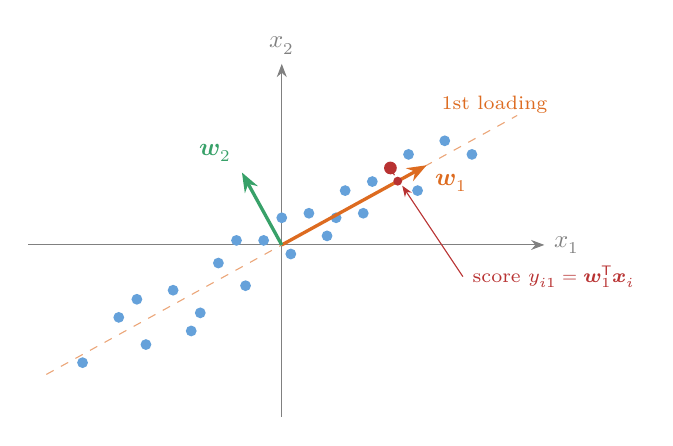
\begin{tikzpicture}[scale=1.15]
  \draw[-{Stealth}, gray] (-2.8,0) -- (2.9,0) node[right] {\small $x_1$};
  \draw[-{Stealth}, gray] (0,-1.9) -- (0,2.0) node[above] {\small $x_2$};
  \foreach \x/\y in {-2.2/-1.3,-1.8/-0.8,-1.5/-1.1,-1.2/-0.5,-0.9/-0.75,-0.7/-0.2,-0.4/-0.45,-0.2/0.05,0.1/-0.1,0.3/0.35,0.5/0.1,0.7/0.6,0.9/0.35,1.2/0.85,1.5/0.6,1.8/1.15,2.1/1.0,-1.0/-0.95,0.0/0.3,0.6/0.3,1.0/0.7,-0.5/0.05,1.4/1.0,-1.6/-0.6}
     \fill[dataC!75] (\x,\y) circle (1.7pt);
  \draw[dashed, accentC!60] (-2.6,-1.43) -- (2.6,1.43);
  \draw[-{Stealth[length=7pt]}, very thick, accentC] (0,0) -- (1.6,0.88) node[below right=-1pt] {\small $\vw_1$};
  \draw[-{Stealth[length=7pt]}, very thick, accentD] (0,0) -- (-0.44,0.8) node[above left] {\small $\vw_2$};
  % projection of a point
  \fill[thmred] (1.2,0.85) circle (2pt);
  \coordinate (P) at (1.2,0.85);
  \coordinate (Pp) at ($(0,0)!(P)!(1.6,0.88)$);
  \draw[thmred, thin, dashed] (P) -- (Pp);
  \fill[thmred] (Pp) circle (1.4pt);
  \node[thmred, font=\scriptsize, right] at (2.0,-0.35) {score $y_{i1}=\vw_1\T\vx_i$};
  \draw[thmred, -{Stealth[length=4pt]}, thin] (2.0,-0.35) -- ($(Pp)+(0.05,-0.05)$);
  \node[accentC, font=\scriptsize] at (2.35,1.55) {1st loading};
\end{tikzpicture}
\caption{Centered data cloud. The first loading $\vw_1$ points along the greatest
variance. $\vw_2\perp\vw_1$ takes the remaining variance. The score of a point is
the signed length of its projection onto each loading.}
\end{figure}

\subsection{The four properties of PCA scores}

\begin{theorem}{PCA scores}{scores}
The score matrix $Y=HXW$ satisfies:
\begin{enumerate}[nosep,label=\arabic*)]
\item \textbf{centered:} $\bar{\vy}=\bm 0$;
\item \textbf{uncorrelated coordinates:} $\Sig_Y$ is diagonal;
\item \textbf{ordered by decreasing variance:} $\Sig_Y=\Lambda=\diag(\lambda_1\ge\cdots\ge\lambda_d)$;
\item \textbf{total variation is preserved:} $\tr(\Sig_Y)=\tr(\Sig_X)$.
\end{enumerate}
\end{theorem}
\begin{proofsketch}
(1) The mean of the scores is
\[
\bar{\vy}=\frac1N\sum_i\vy_i=\frac1N Y\T\one=\frac1N W\T X\T H\T\one=\frac1N W\T X\T(\underbrace{H\one}_{=\bm0})=\bm0 .
\]
(2)--(3) Because the scores are centered, $\Sig_Y=\tfrac1N Y\T Y-\bar{\vy}\bar{\vy}\T=\tfrac1N Y\T Y$, and
\[
\Sig_Y=\frac1N(HXW)\T(HXW)=W\T\Big(\tfrac1N X\T H\T H X\Big)W=W\T\Sig_X W=\underbrace{W\T W}_{I}\,\Lambda\,\underbrace{W\T W}_{I}=\Lambda .
\]
We used $H\T H=H^2=H$ and $W^{-1}=W\T$.
(4) $\tr(\Lambda)=\tr(W\Lambda W\T)=\tr(\Sig_X)$ by the cyclic property of the trace.
\end{proofsketch}

\begin{intuition}
$\tr(\Sig_X)=\sum_j\operatorname{Var}(\text{feature } j)=\frac1N\sum_i\norm{\vx_i-\xbar}^2$
is the \textbf{total variation} in $\vx_1,\dots,\vx_N$. A rotation cannot create or
destroy spread. It only redistributes it among the axes. PCA picks the rotation that
packs as much variance as possible into the first axis, then the second, and so on.

At this stage PCA maps a $d$-vector to a $d$-vector: \textbf{no dimension reduction
has happened yet}. It is a change of basis.
\end{intuition}

\subsection{PCA as a greedy search for variance}

The variance of the scores along a unit direction $\vw$ is
$\frac1N\sum_i\big(\vw\T(\vx_i-\xbar)\big)^2=\vw\T\Sig\vw$. By the Rayleigh quotient
(Prop.~\ref{prop:rayleigh}):
\[
\vw_1=\argmax_{\norm{\vw}=1}\vw\T\Sig\vw,\qquad
\vw_2=\argmax_{\norm{\vw}=1,\ \vw\perp\vw_1}\vw\T\Sig\vw,\qquad\dots
\]
\textbf{Remove the maximum variance each time and then go orthogonally.} Each step can
only find less variance than the one before, so the components come out in decreasing
order of variance automatically.

\begin{theorem}{What PCA does, in one sentence}{pcasummary}
Given data in $\R^d$, PCA
\begin{enumerate}[nosep,label=\arabic*)]
\item learns an orthonormal basis $\vw_1,\dots,\vw_d$ (new axes, centered at $\xbar$), and
\item expresses each centered $\vx_i$ in that basis: $\vy_i=(\vx_i\T\vw_1,\dots,\vx_i\T\vw_d)\T$
are \emph{the coordinates of $\vx_i$ in the learned basis}.
\end{enumerate}
\end{theorem}

\begin{example}{The classic $2\times2$: $\Sig=\begin{bmatrix}a&b\\b&a\end{bmatrix}$}{abba}
\textbf{Question.} Find the PC variances, the loadings, and the proportion of variance explained by PC1.

\textbf{PC variances (eigenvalues).} Solve $\det(\Sig-\lambda I)=0$:
\[
(a-\lambda)^2-b^2=0\ \Longrightarrow\ a-\lambda=\pm b\ \Longrightarrow\ \lambda=a+b\quad\text{or}\quad\lambda=a-b .
\]
For $\Sig$ to be a valid covariance matrix (PSD) you need $a\ge|b|$, so both are $\ge0$. Strictly $a>|b|$ makes both positive
(positive definite). At $a=|b|$ one variance is $0$ and the data lie on a line.

\textbf{Loadings (eigenvectors).} For $\lambda=a+b$: $(\Sig-\lambda I)\bm e=\bm0$ reads $-b\,e_1+b\,e_2=0$, so $e_1=e_2$, and normalizing
gives $\bm e=\tfrac1{\sqrt2}(1,1)$, i.e.\ $Y=\tfrac{X_1+X_2}{\sqrt2}$. For $\lambda=a-b$: $b\,e_1+b\,e_2=0$, so $e_1=-e_2$, giving $\bm e=\tfrac1{\sqrt2}(1,-1)$, i.e.\ $Y=\tfrac{X_1-X_2}{\sqrt2}$.
(Dividing by $b$ assumes $b\ne0$; see the last bullet.)

\textbf{Which comes first depends on the sign of $b$.}
\begin{itemize}[nosep]
\item $b>0$ (positive correlation): PC1 $=\tfrac{X_1+X_2}{\sqrt2}$ with variance $a+b$, explaining
$\dfrac{a+b}{(a+b)+(a-b)}=\dfrac{a+b}{2a}=\tfrac12+\dfrac{b}{2a}$.
\item $b<0$ (negative correlation): the roles swap. PC1 $=\tfrac{X_1-X_2}{\sqrt2}$ with variance $a-b$, explaining $\dfrac{a-b}{2a}$.
\item Both cases: $\boxed{\text{PVE}_1=\dfrac{a+|b|}{2a}=\tfrac12+\tfrac12|\rho|}$, where $\rho=b/a$ is the correlation of $X_1$ and $X_2$.
\item $b=0$: $\Sig=aI$, a tie. Both PCs explain exactly half, and \emph{every} direction is a valid loading (the circle, Example~\ref{ex:pcacircle}).
\end{itemize}
\end{example}

\begin{intuition}
\textbf{The loadings never depend on $a$ or $b$.} Because the two variables have equal variance, swapping them leaves $\Sig$
unchanged, and that symmetry forces the principal axes onto the $45^\circ$ diagonals: the sum and the difference of the
variables. Only the \emph{order} (set by the sign of $b$) and the \emph{sizes} change. As $|\rho|\to1$ the cloud collapses onto a
diagonal line and PC1 explains nearly everything, while $\rho=0$ gives a round cloud with no preferred direction. Throughout,
the total variance is $\tr\Sig=2a$ whatever $b$ is: PCA only \emph{redistributes} it between the two directions
(Theorem~\ref{thm:scores}). Cross-check with Example~\ref{ex:covbyhand}: there $\Sig=\begin{bmatrix}2/3&-1/3\\-1/3&2/3\end{bmatrix}$, so $a=\tfrac23$, $b=-\tfrac13$, giving
$\lambda=a-b=1$ for PC1 $\propto(1,-1)$ and $\lambda=a+b=\tfrac13$, with PVE $=\tfrac{a+|b|}{2a}=\tfrac34$. This matches the values computed there.
If the variances are \emph{unequal} the symmetry breaks and the axes tilt toward the higher-variance variable,
which is the scale-sensitivity issue of Section~2.6.
\end{intuition}

\subsection{Covariance, correlation and rescaling}

\begin{definition}{Correlation}{corr}
$\displaystyle \operatorname{cor}(x_1,x_2)=\frac{\operatorname{cov}(x_1,x_2)}{\sqrt{\operatorname{Var}(x_1)\operatorname{Var}(x_2)}}\in[-1,1]$.
Correlation is covariance with the units divided out.
\end{definition}

\begin{proposition}{Rescaling the variables}{rescale}
If each variable is rescaled, $Y=XD$ with $D=\diag(c_1,\dots,c_d)$, then
\[
\Sig_Y=\tfrac1N Y\T Y=\tfrac1N(XD)\T(XD)=D\T\Big(\tfrac1N X\T X\Big)D=D\T\Sig_X D .
\]
Entry $(j,k)$ is multiplied by $c_jc_k$. Variances scale by $c_j^2$.
\end{proposition}

\begin{proposition}{Covariance under any linear map plus shift}{covaffine}
If a random vector $\vx$ has mean $\bm\mu$ and covariance $\Sigma$, then for any matrix $A$ and constant vector $\bm b$,
\[
\operatorname{Cov}(A\vx+\bm b)=A\Sigma A\T .
\]
\end{proposition}
\begin{proofsketch}
Let $\vy=A\vx+\bm b$. Its mean is $\mathbb E\vy=A\bm\mu+\bm b$, so $\vy-\mathbb E\vy=A(\vx-\bm\mu)$. The $\bm b$'s cancel. Then
\[
\operatorname{Cov}(\vy)=\mathbb E\big[A(\vx-\bm\mu)(\vx-\bm\mu)\T A\T\big]=A\,\mathbb E\big[(\vx-\bm\mu)(\vx-\bm\mu)\T\big]A\T=A\Sigma A\T,
\]
using $(A\bm v)\T=\bm v\T A\T$ and pulling the constant matrices out of the expectation.
\end{proofsketch}

\begin{intuition}
In one dimension this is $\operatorname{Var}(ax+b)=a^2\operatorname{Var}(x)$: shifting does nothing to spread, and
scaling by $a$ scales variance by $a^2$. The matrix version puts one $A$ on each side because
covariance compares the output with \emph{itself}: one copy of the deviation is transformed by $A$,
the other by $A\T$. Rescaling ($A=D$) and PCA ($A=W\T$, giving $W\T\Sig W=\Lambda$) are both special
cases. A common slip is to write an extra $\bm b\bm b\T$. That term belongs to the
\emph{uncentered} second moment $\mathbb E[\vy\vy\T]$, not to the covariance.
\end{intuition}

\begin{deeper}
Choose $c_j=1/s_j$ (one over the standard deviation). This \emph{standardizes} the data,
and $D\Sig_X D$ becomes the \textbf{correlation matrix}. So ``PCA on standardized data''
and ``eigendecomposition of the correlation matrix'' are the same thing.
\end{deeper}

\begin{example}{Guessing a variance from a range}{range}
Suppose a variable lives in $[0,2]$ and looks roughly normal. About 95\% of a normal
lies within $\pm2\sigma$, so match $[\mu-2\sigma,\mu+2\sigma]\approx[0,2]$:
$4\sigma=2$, giving $\sigma=0.5$ and $\sigma^2=0.25$.
\end{example}

\subsection{Weaknesses of PCA}

PCA relies on \textbf{variance} and \textbf{linear approximation}. Each one brings a weakness.
\begin{enumerate}[label=\roman*)]
\item \textbf{Variance is sensitive to different scales and to outliers.} Units determine variance directly.
\item \textbf{Nonlinear structure:} PCA can only find flat (affine) structure, so it cannot
detect a curve or a curved surface (Section~\ref{sec:kpca}).
\end{enumerate}

\begin{figure}[htbp]
\centering
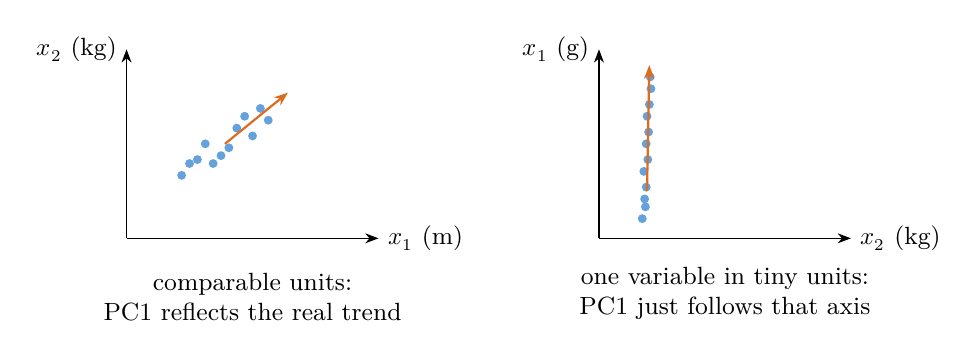
\begin{tikzpicture}
\begin{scope}
  \draw[-{Stealth}] (0,0) -- (3.2,0) node[right] {\small $x_1$ (m)};
  \draw[-{Stealth}] (0,0) -- (0,2.4) node[left] {\small $x_2$ (kg)};
  \foreach \x/\y in {0.7/0.8,0.9/1.0,1.1/0.95,1.0/1.2,1.3/1.15,1.4/1.4,1.6/1.3,1.2/1.05,1.5/1.55,1.8/1.5,0.8/0.95,1.7/1.65}
     \fill[dataC!75] (\x,\y) circle (1.6pt);
  \draw[-{Stealth[length=5pt]}, thick, accentC] (1.25,1.2) -- (2.05,1.85);
  \node[font=\small, align=center] at (1.6,-0.75) {comparable units:\\ PC1 reflects the real trend};
\end{scope}
\begin{scope}[xshift=6cm]
  \draw[-{Stealth}] (0,0) -- (3.2,0) node[right] {\small $x_2$ (kg)};
  \draw[-{Stealth}] (0,0) -- (0,2.4) node[left] {\small $x_1$ (g)};
  \foreach \x/\y in {0.55/0.25,0.58/0.5,0.6/0.65,0.57/0.85,0.62/1.0,0.6/1.2,0.63/1.35,0.61/1.55,0.64/1.7,0.66/1.9,0.59/0.4,0.65/2.05}
     \fill[dataC!75] (\x,\y) circle (1.6pt);
  \draw[-{Stealth[length=5pt]}, thick, accentC] (0.61,0.6) -- (0.64,2.2);
  \node[font=\small, align=center] at (1.6,-0.7) {one variable in tiny units:\\ PC1 just follows that axis};
\end{scope}
\end{tikzpicture}
\caption{Scale imbalance. Re-expressing one variable in smaller units multiplies its
variance by a huge constant, and PC1 snaps onto that axis no matter what the real
structure is.}
\end{figure}

\begin{intuition}
The fix is to \textbf{standardize} the data, which puts every variable on unit variance.
Sometimes a \textbf{variance-stabilising transform} (e.g.\ $\log$ for counts or
right-skewed data) is better than standardizing. It shrinks the influence of extreme
values instead of only rescaling them.
\end{intuition}

\subsubsection*{Weakness (ii) in detail: covariance only sees linear relationships}

\textbf{Linear dependence is visible to PCA.} If one feature is an exact linear
combination of others, say $x_3=2x_1+x_2$, then the vector $\vw\propto(2,1,-1)$
satisfies $\vw\T\vx=0$ for every point. The variance along $\vw$ is zero, so
$\Sig$ has a zero eigenvalue and $\rank(HX)=2$. PCA correctly reports ``three columns,
two dimensions''.

\textbf{Nonlinear dependence can be invisible.} Take $x\in\{-2,-1,0,1,2\}$ and
$y=x^2\in\{4,1,0,1,4\}$. Here $y$ is a perfect function of $x$, yet
\[
\operatorname{cov}(x,y)=\tfrac15\sum_i(x_i-0)(y_i-2)=\tfrac15\big[(-2)(2)+(-1)(-1)+0+(1)(-1)+(2)(2)\big]=0 .
\]
Covariance measures only \emph{linear} association, and for data symmetric around zero
the linear trend of $x^2$ on $x$ is exactly flat. Both PC variances are positive, so PCA
reports two dimensions for points that lie on a one-dimensional curve.

\begin{intuition}
Keep two notions of ``low-dimensional'' apart:
\begin{itemize}[nosep]
\item \textbf{linear} low-dimensionality: the points lie in a flat subspace (visible as zero or small $\lambda$'s);
\item \textbf{intrinsic} (nonlinear) low-dimensionality: the points lie on a curved set with few degrees of freedom.
\end{itemize}
PCA detects only the first. A low-rank feature matrix tells you that some features are
\emph{linearly redundant}. It does not tell you how many degrees of freedom actually
generated the data.
\end{intuition}

\begin{deeper}
\textbf{How to tell whether PCA missed nonlinear structure.} (1) Plot the scores
(PC1 vs PC2, PC2 vs PC3). Curves, arcs, rings, spirals and ``horseshoes'' are signs of
a curved set seen through a linear lens. (2) Compare reconstruction error with the
number of PCs. A curve needs several PCs to reach small error even though it has one
degree of freedom. (3) Run a nonlinear method (kernel PCA, Section~\ref{sec:kpca}) and see
whether it finds a much simpler description. (4) Measure dependence in ways that are not
limited to linear relationships, such as mutual information or distance correlation.
\textbf{Mild} curvature does not ruin PCA. The best flat approximation of a gently bent
cloud can still be excellent. PCA gives the best \emph{linear} approximation, which may
or may not be the true structure.
\end{deeper}

% ==================================================================
\section{Dimension Reduction with PCA}
% ==================================================================

\subsection{Rank-$k$ approximation}

Since $W$ is orthogonal, every data point is \emph{exactly} recovered from all $d$ scores:
\[
\vx_i=\xbar+\sum_{j=1}^{d}y_{ij}\vw_j .
\]
For a rank-$k$ approximation we keep only the first $k$ scores, which hold the most
important variation:
\[
\widehat{\vx}_i^{(k)}=\xbar+y_{i1}\vw_1+\cdots+y_{ik}\vw_k\ \in\ \xbar+\spn\{\vw_1,\dots,\vw_k\},
\]
a $k$-dimensional affine hyperplane. The vector
$\vy_i^{(k)}=(y_{i1},\dots,y_{ik})$ is the \textbf{$k$-dimensional representation} of
$\vx_i$: we have reduced $d\to k$. Using more PCs gives a better approximation, and
with all $d$ we restore the exact vector.

\textbf{Matrix form.} Stack the scores $Y=HXW$ (centered data times loadings). Since $W$ is orthogonal, $HX=YW\T$, and
adding the mean back to every row gives
\[
X=YW\T+\one_N\xbar\T,\qquad
\widehat X^{(k)}=Y^{(k)}W^{(k)\T}+\one_N\xbar\T,\qquad
\Fro{X-\widehat X^{(k)}}^2=N\sum_{j>k}\lambda_j ,
\]
where $Y^{(k)}$ and $W^{(k)}$ keep the first $k$ columns. The term $\one_N\xbar\T$ ($N\times1$ times $1\times d$) is exactly ``adding
back the centering'': it puts the mean row $\xbar\T$ back on every sample. (Watch the order: $\xbar\T\one_N$ would not
even be defined as a matrix of the right shape.) The error is the discarded variance times $N$ (Theorem~\ref{thm:bestsub}).

\begin{definition}{Linear vs.\ affine subspace}{affinedef}
A \textbf{linear subspace} is a set $V=\spn\{\bm v_1,\dots,\bm v_k\}$. It always contains the
origin (take all coefficients $0$) and is closed under adding vectors and scaling them. An
\textbf{affine subspace} is a translated linear subspace, $\bm a+V=\{\bm a+\bm v:\bm v\in V\}$.
It is a flat (line, plane, \dots) that need not pass through the origin. Its dimension is $\dim V$.
\end{definition}

\begin{example}{Two points in $\R^3$}{twopoints}
Any two points $\vx_1\ne\vx_2$ lie on the line $\{\vx_1+t(\vx_2-\vx_1):t\in\R\}$. This is a
$1$-dimensional \emph{affine} subspace, and it generally misses the origin, so it is not a linear
subspace. After centering, $\vx_1-\xbar=-(\vx_2-\xbar)$, and the two centered points lie on the
\emph{linear} subspace $\spn\{\vx_2-\vx_1\}$. Centering turns ``best affine flat'' into ``best linear
subspace'', which is why PCA can work with $\spn\{\vw_1,\dots,\vw_k\}$ and just add $\xbar$ back.
\end{example}

\subsection{Optimality of PCA}

\begin{theorem}{PCA gives the best $k$-dimensional subspace}{bestsub}
Assume $\vx_1,\dots,\vx_N$ are centered. For \emph{any} $k$-dimensional linear subspace
$V\subseteq\R^d$, with $\proj_V$ the orthogonal projection,
\[
\frac1N\sum_{i=1}^N\norm{\vx_i-\proj_V(\vx_i)}^2\ \ge\ \lambda_{k+1}+\cdots+\lambda_d ,
\]
with equality when $V=\spn\{\vw_1,\dots,\vw_k\}$.
\end{theorem}
\begin{proofsketch}
Let $P=QQ\T$ be the projector onto $V$, where $Q\in\R^{d\times k}$ has orthonormal columns.
Since $I-P$ is a symmetric projector,
\[
\tfrac1N\sum_i\norm{(I-P)\vx_i}^2=\tfrac1N\sum_i\vx_i\T(I-P)\vx_i=\tr\big((I-P)\Sig\big)=\tr\Sig-\tr(Q\T\Sig Q).
\]
Expanding $\Sig=\sum_j\lambda_j\vw_j\vw_j\T$ gives $\tr(Q\T\Sig Q)=\sum_j\lambda_j c_j$ with
$c_j=\norm{Q\T\vw_j}^2$. Each $c_j\in[0,1]$, and $\sum_j c_j=\tr(QQ\T)=k$. A sum
$\sum\lambda_jc_j$ under these constraints is largest when $c_1=\cdots=c_k=1$ and the
rest are $0$, giving $\lambda_1+\cdots+\lambda_k$. Therefore the residual is at least
$\sum_j\lambda_j-\sum_{j\le k}\lambda_j=\sum_{j>k}\lambda_j$.
\end{proofsketch}

\begin{corollary}{Removing the centering assumption}{affine}
Given any $k$-dimensional \emph{affine} subspace $V$ (a translated hyperplane) with
orthogonal projection $\proj_V$,
\[
\frac1N\sum_{i=1}^N\norm{\vx_i-\proj_V(\vx_i)}^2\ \ge\ \lambda_{k+1}+\cdots+\lambda_d ,
\]
with equality for $V=\xbar+\spn\{\vw_1,\dots,\vw_k\}$.
\end{corollary}
\begin{proofsketch}
Write $V=\bm a+V_0$ with $V_0$ linear and projector $P$. Then
$\vx_i-\proj_V(\vx_i)=(I-P)(\vx_i-\bm a)=(I-P)(\vx_i-\xbar)+(I-P)(\xbar-\bm a)$.
When we average the squared norm, the cross term vanishes because
$\sum_i(\vx_i-\xbar)=\bm0$, leaving
\[
\tfrac1N\sum_i\norm{(I-P)(\vx_i-\xbar)}^2+\norm{(I-P)(\xbar-\bm a)}^2 .
\]
The second piece is $\ge0$, so the best translation passes through $\xbar$, and the first
piece is bounded by the theorem.
\end{proofsketch}

\begin{intuition}
Fitting the best affine hyperplane is a two-step problem. First translate it through the
mean, which is what centering ``undoes''. Then rotate it toward the top eigenvectors.
The leftover error is exactly the variance in the directions you threw away.
\end{intuition}

\subsection{When some PC variances are zero: exact low-dimensional structure}

Suppose $\lambda_1,\dots,\lambda_j>0$ and $\lambda_{j+1}=\cdots=\lambda_d=0$. A zero
variance along $\vw_s$ means \emph{every} point has $\vw_s\T(\vx_i-\xbar)=0$. So the
data lie \emph{exactly} on a $j$-dimensional affine hyperplane, and there are two
equivalent ways to describe it:
\[
\underbrace{\xbar+\spn\{\vw_1,\dots,\vw_j\}}_{\substack{\text{explicit definition of the}\\\text{affine hyperplane containing the data}}}
\;=\;
\underbrace{\big\{\bm v:\ \vw_s\T(\bm v-\xbar)=0\ \text{for all } s>j\big\}}_{\substack{\text{implicit description:}\\ d-j \text{ linear equations}}} .
\]
The PC scores $y_{i\ell}=\vw_\ell\T(\vx_i-\xbar)$, $\ell=1,\dots,j$, are coordinates of the data
\emph{inside} that hyperplane. The geometry, or rank, is smaller than you think.

\begin{proposition}{At most $N-1$ nonzero PC variances}{nminus1}
$\rank(HX)\le\min(N-1,d)$, so at most $N-1$ of the $\lambda$'s are positive.
\end{proposition}
\begin{proofsketch}
$HX$ has $d$ columns, so its rank is at most $d$. For the $N-1$ bound, use
Prop.~\ref{prop:Hprops}(iv): $(HX)\T\one=\bm0$, so the nonzero vector $\one$ lies in
the null space of the $d\times N$ matrix $(HX)\T$. Rank--nullity for $(HX)\T$ gives
$\rank(HX)\T+\dim\operatorname{null}(HX)\T=N$ with $\dim\operatorname{null}\ge1$, so
$\rank(HX)=\rank(HX)\T\le N-1$. Finally, $\Sig=\tfrac1N(HX)\T(HX)$ has the same rank as
$HX$, and the rank of a symmetric matrix is its number of nonzero eigenvalues.
\end{proofsketch}

\begin{intuition}
\textbf{One constraint costs one dimension.} For each feature the deviations
$x_{1j}-\bar x_j,\dots,x_{Nj}-\bar x_j$ sum to zero. So if you know $N-1$ of them, the
last one is forced. If the first two deviations are $-1$ and $2$, the third must be
$-1$. The centered rows carry only $N-1$ independent pieces of information. Geometrically,
$N$ points always fit inside an $(N-1)$-dimensional affine subspace: two points lie on a
line, three on a plane, and so on. For example, $2$ points in $\R^3$ always lie on a line,
so only $\lambda_1>0$.
\end{intuition}

\begin{example}{More features than samples}{nlessd}
With $N=5$ patients and $d=10$ genes, $\rank(HX)\le\min(4,10)=4$. At most $4$ of
the $10$ PC variances are nonzero, whatever the data. The other six are zero because there
are not enough samples to spread in more directions, not because of real structure. With
$N=20$ and $d=1000$, PCA still runs, but it estimates a $1000\times1000$ covariance from
$20$ points and finds at most $19$ nonzero directions.
\end{example}

\begin{deeper}
\textbf{How much data is ``enough'' for PCA?} There is no single cutoff. $N\gg d$ is
comfortable, and $N\lesssim d$ makes the estimated loadings unstable. A practical test
asks whether the top loadings look the same on another sample. You can check by
bootstrapping, refitting on random subsets, or comparing train/test PCs. If the first few
loadings change a lot when you drop $10\%$ of the samples, don't interpret them.
\end{deeper}

\begin{careful}
\textbf{Samples vs.\ features: what ``$N-1$'' does and does not say.} The bound
$\rank(HX)\le\min(N-1,d)$ has two parts, and only the smaller one matters.
\begin{itemize}[nosep]
\item If $N>d$ (more samples than features, the usual case), the bound is $d$. The $N-1$ is
irrelevant: $1000$ points in $\R^3$ have at most $3$ nonzero PC variances, not $999$.
\item If $N\le d$, the bound is $N-1$. You can \emph{always} describe centered data with $N-1$
coordinates, whatever $d$ is, because $N$ points span at most an $(N-1)$-dimensional affine
flat.
\end{itemize}
Neither bound says how many dimensions you \emph{need}. That is the number of large
$\lambda$'s, which can be far smaller than both. Also, $N-1$ is not a number of \emph{features}.
It counts directions in $\R^d$ that the samples can spread along. Each such direction is a
combination of all $d$ original features.
\end{careful}

\begin{intuition}
\textbf{Does more data raise the rank?} Only if the new point leaves the current flat. Centered
points $(1,1),(2,2),(3,3)$ vary along one direction (rank $1$). Adding $(4,4)$ gives more evidence
about that same direction, and the rank stays $1$. Adding $(2,5)$, which is off the line, shows a
new kind of variation, and the rank can become $2$. More samples raise the \emph{ceiling}
$\min(N-1,d)$, not necessarily the rank itself. Also separate the \textbf{algebraic rank}
(the number of nonzero $\lambda$'s, usually all of them for noisy data) from the \textbf{effective
rank} (the number of $\lambda$'s that are large enough to matter, read off a scree plot).
\end{intuition}

\begin{careful}
Clear separations of magnitude (a sharp drop to zero) rarely occur with real data.
Noise makes every $\lambda$ positive, so we have to judge where the eigenvalues become
``small''.
\end{careful}

\subsection{Assessing PCA and choosing $k$}

To assess a PCA, look at three things: the \textbf{loadings} (what each axis means),
the \textbf{scores} (where each sample sits, typically in 2D/3D scatter plots), and the
\textbf{variances} (how much each axis matters).

\textbf{Q: How many dimensions should I reduce to?}

\begin{figure}[htbp]
\centering
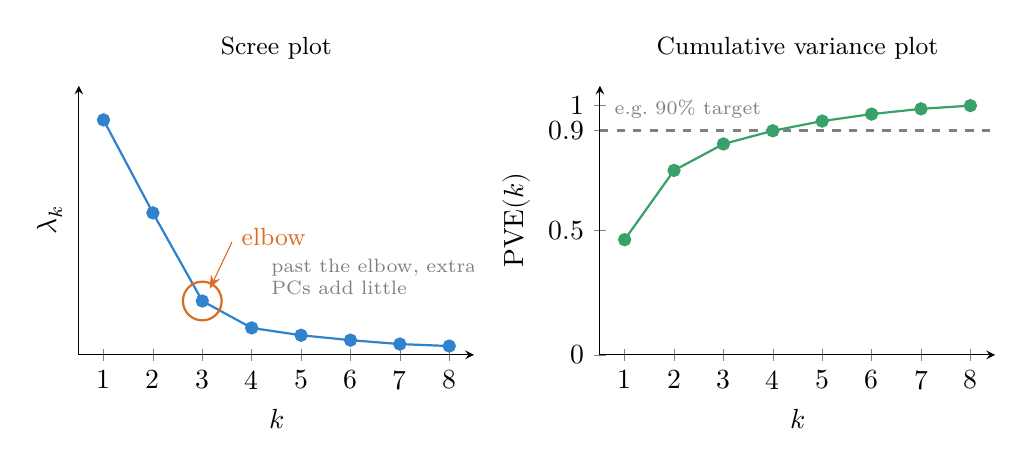
\begin{tikzpicture}
\begin{axis}[name=scree, width=6.6cm, height=5cm, xlabel={$k$}, ylabel={$\lambda_k$}, title={\small Scree plot},
  xmin=0.5, xmax=8.5, ymin=0, ymax=5.5, xtick={1,...,8}, ytick=\empty, axis lines=left, every axis plot/.append style={thick}]
  \addplot[mark=*, color=dataC] coordinates {(1,4.8)(2,2.9)(3,1.1)(4,0.55)(5,0.4)(6,0.3)(7,0.22)(8,0.18)};
  \draw[accentC, thick] (axis cs:3,1.1) circle (7pt);
  \node[accentC, font=\small, anchor=west] at (axis cs:3.6,2.4) {elbow};
  \draw[accentC, -{Stealth}] (axis cs:3.6,2.3) -- (axis cs:3.15,1.35);
  \node[font=\scriptsize, gray, anchor=west, align=left] at (axis cs:4.2,1.6) {past the elbow, extra\\ PCs add little};
\end{axis}
\begin{axis}[at={(scree.east)}, anchor=west, xshift=1.6cm, width=6.6cm, height=5cm, xlabel={$k$}, ylabel={PVE$(k)$},
  title={\small Cumulative variance plot}, xmin=0.5, xmax=8.5, ymin=0, ymax=1.08, xtick={1,...,8}, ytick={0,0.5,0.9,1}, axis lines=left, every axis plot/.append style={thick}]
  \addplot[mark=*, color=accentD] coordinates {(1,0.462)(2,0.740)(3,0.846)(4,0.899)(5,0.938)(6,0.966)(7,0.987)(8,1.0)};
  \addplot[dashed, gray] coordinates {(0.5,0.9)(8.5,0.9)};
  \node[font=\scriptsize, gray, anchor=south west] at (axis cs:0.6,0.91) {e.g.\ 90\% target};
\end{axis}
\end{tikzpicture}
\caption{Two standard diagnostics. \textbf{Left:} the scree plot of $\lambda_k$ against $k$.
Look for the elbow, where variability stops dropping quickly. \textbf{Right:} the cumulative
proportion of variance. Choose the smallest $k$ that explains enough of the variance.}
\end{figure}

\begin{definition}{Proportion of variance explained}{pve}
\[
\text{PVE}(k)=\frac{\sum_{j=1}^k\lambda_j}{\sum_{j=1}^d\lambda_j}
=\frac{\text{variance kept by the first } k\text{ PCs}}{\text{total variance}}
=1-\frac{\text{reconstruction error of rank } k}{\text{total variance}} .
\]
\end{definition}

\begin{example}{Reading a gap in the scree plot}{gap}
Suppose the scree plot has three large eigenvalues followed by a big gap. There are
three possible stories, and you have to work out which one applies:
\begin{enumerate}[nosep]
\item the data really (approximately) live in a 3-dimensional affine hyperplane;
\item the \textbf{data scale is wrong}: three variables measured in tiny units dominate the variance (fix: standardize);
\item there are \textbf{3 outliers}. Each extreme point can grab its own high-variance direction.
\end{enumerate}
\end{example}

% ==================================================================
\section{The Singular Value Decomposition}\label{sec:svd}
% ==================================================================

\subsection{Definition and shapes}

\begin{theorem}{SVD}{svd}
Every $A\in\R^{m\times n}$ factors as $A=USV\T$ where
\begin{itemize}[nosep]
\item $U\in\R^{m\times m}$ is orthogonal; its columns $\vu_i$ are the \textbf{left singular vectors};
\item $V\in\R^{n\times n}$ is orthogonal; its columns $\vv_i$ are the \textbf{right singular vectors};
\item $S\in\R^{m\times n}$ is ``diagonal'' with $\sigma_1\ge\cdots\ge\sigma_r>0$ followed by zeros.
\end{itemize}
Then $\rank(A)=r$, $\col(A)=\spn\{\vu_1,\dots,\vu_r\}$ and
$\operatorname{null}(A)=\spn\{\vv_{r+1},\dots,\vv_n\}$, which has dimension $n-r$.
\end{theorem}

\begin{figure}[htbp]
\centering
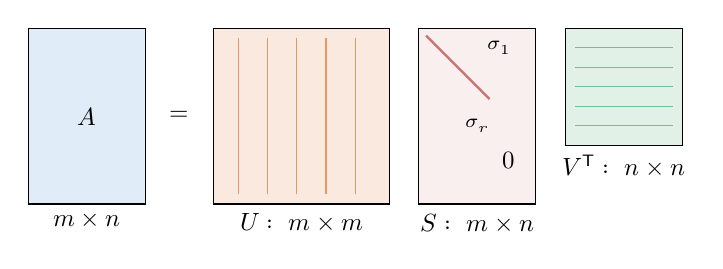
\begin{tikzpicture}[scale=0.62, every node/.style={font=\small}]
  \draw[fill=dataC!15] (0,0) rectangle (2.4,3.6); \node at (1.2,1.8) {$A$};
  \node[below] at (1.2,0) {$m\times n$};
  \node at (3.1,1.8) {$=$};
  \draw[fill=accentC!15] (3.8,0) rectangle (7.4,3.6);
  \foreach \x in {4.3,4.9,5.5,6.1,6.7} \draw[accentC!70] (\x,0.2) -- (\x,3.4);
  \node[below] at (5.6,0) {$U:\ m\times m$};
  \draw[fill=thmred!8] (8.0,0) rectangle (10.4,3.6);
  \draw[thmred!70, thick] (8.15,3.45) -- (9.45,2.15);
  \node[font=\scriptsize] at (9.65,3.2) {$\sigma_1$};
  \node[font=\scriptsize] at (9.2,1.6) {$\sigma_r$};
  \node at (9.85,0.9) {$0$};
  \node[below] at (9.2,0) {$S:\ m\times n$};
  \draw[fill=accentD!15] (11.0,1.2) rectangle (13.4,3.6);
  \foreach \y in {1.6,2.0,2.4,2.8,3.2} \draw[accentD!70] (11.2,\y) -- (13.2,\y);
  \node[below] at (12.2,1.2) {$V\T:\ n\times n$};
\end{tikzpicture}
\caption{Shapes in the full SVD of a tall matrix ($m>n$). Only the first $r$ singular values are nonzero.}
\end{figure}

\subsection{Connection to eigendecompositions}

\begin{proposition}{SVD $\leftrightarrow$ EVD of $A\T A$}{svdevd}
\[
A\T A=(VS\T U\T)(USV\T)=V\,S\T S\,V\T=V\begin{bmatrix}\sigma_1^2&&\\&\ddots&\\&&\sigma_n^2\end{bmatrix}V\T .
\]
This is the eigendecomposition of $A\T A$. Its eigenvectors are the \textbf{right singular
vectors} of $A$, and its eigenvalues are the squared singular values. Similarly
$AA\T=U\,SS\T\,U\T$, whose eigenvectors are the left singular vectors. Also
$AV=US$, i.e.\ $A\vv_i=\sigma_i\vu_i$.
\end{proposition}

\subsection{PCA via the SVD}\label{sec:pcasvd}

Apply the SVD to the centered data, $HX=USV\T$. Then
\[
\Sig=\tfrac1N(HX)\T(HX)=V\Big(\tfrac1N S\T S\Big)V\T
\quad\Longrightarrow\quad
W=V,\qquad \lambda_j=\frac{\sigma_j^2}{N},\qquad Y=HXV=US .
\]
The loadings are the right singular vectors, the PC variances are the squared singular
values divided by $N$, and the scores are $US$. Each nonzero $\sigma$ corresponds to a PC.

\begin{careful}
The notes say ``$\sigma_i^2=$ variance''. More precisely $\lambda_i=\sigma_i^2/N$, or $\sigma_i^2/(N-1)$
with the other convention. This only matters when you report actual variances.
Proportions such as PVE are unaffected.
\end{careful}

\subsection{What happens to the SVD under rotations and permutations}

\begin{proposition}{Products of orthogonal matrices are orthogonal}{orthprod}
If $B,C$ are orthogonal then $(BC)\T(BC)=C\T B\T BC=C\T C=I$.
\end{proposition}

\begin{example}{Rotating the features}{rot}
Let $\vz_i\T=\vx_i\T Q$ for an orthogonal $Q$, i.e.\ $Z=XQ$. If $X=U\Sigma V\T$, then
\[
Z=U\Sigma V\T Q=U\Sigma(Q\T V)\T .
\]
$Q\T V$ is orthogonal, so this \emph{is} an SVD of $Z$. The singular values and the left
singular vectors are unchanged, so \textbf{the PC scores and variances are rotation invariant}.
The loadings simply rotate along: $V\mapsto Q\T V$.
\end{example}

\begin{example}{Permuting the samples}{perm}
Reordering rows is $PX$ with $P$ a permutation (hence orthogonal) matrix:
$PX=(PU)\Sigma V\T$. The left singular vectors change (they get permuted the same way)
because $P$ stays on the left side. The loadings $V$ and the variances are unchanged.
Sample order is irrelevant to PCA, as it should be.
\end{example}

\begin{example}{A $3\times2$ SVD}{svd32}
$A=\begin{bmatrix}1&2\\3&4\\5&6\end{bmatrix}$, so $A=U_{3\times3}S_{3\times2}V\T_{2\times2}$. Row reduction
($r_2-3r_1$, $r_3-5r_1$, \dots) leaves two pivots, so $\rank A=2$ and both singular values are positive.
$A\T A=\begin{bmatrix}35&44\\44&56\end{bmatrix}$ has trace $91$ and determinant $24$, so
$\sigma_{1,2}^2=\tfrac{91\pm\sqrt{8185}}{2}\approx 90.74,\ 0.26$. That gives
$\sigma_1\approx9.53$ and $\sigma_2\approx0.51$. The second direction carries very little of the matrix.
\end{example}

\subsection{Reading the SVD: axes, coordinates and scale}

Take centered data $X\in\R^{N\times d}$ ($N$ samples as rows, $d$ features as columns) with thin
SVD $X=U\Sigma V\T$, where $r=\rank X$, $U\in\R^{N\times r}$, $\Sigma\in\R^{r\times r}$ and $V\in\R^{d\times r}$.
\begin{center}
\renewcommand{\arraystretch}{1.3}
\begin{tabular}{@{}l>{\raggedright\arraybackslash}p{3.4cm}>{\raggedright\arraybackslash}p{6.6cm}@{}}
\toprule
piece & lives in & meaning \\
\midrule
$\vv_j$ (column of $V$) & \textbf{feature space} $\R^d$ & the $j$th new axis, as a recipe of original features \\
$\vu_j$ (column of $U$) & \textbf{sample space} $\R^N$ & how each sample lines up with axis $j$, rescaled to unit length \\
$\sigma_j$ & a number & how much spread lies along axis $j$ (variance $\sigma_j^2/N$) \\
$U\Sigma=XV$ & $\R^{N\times r}$ & every sample's \textbf{coordinates} on the new axes (the PC scores) \\
\bottomrule
\end{tabular}
\end{center}
The link is $X\vv_j=\sigma_j\vu_j$. For example, if $\vv_1=(0.5,0.8,0.3)$ for the features (height,
weight, age), then PC1 is the direction $0.5\cdot\text{height}+0.8\cdot\text{weight}+0.3\cdot\text{age}$, and person
$i$'s PC1 score is $\vx_i\T\vv_1=\sigma_1u_{i1}$.

\begin{intuition}
\textbf{The crayon picture.} Each sample is a drawing described by how much of every original
crayon colour it uses (a row of $X$). PCA notices that a few \emph{mixed} crayons describe most
drawings. $V$ holds the recipes for the new crayons (what each is made of), and $U\Sigma$ says how
much of each new crayon each drawing uses. So $X=(U\Sigma)V\T$ reads ``amounts $\times$ recipes''.
Keeping only the best $k$ crayons gives a slightly simplified drawing that usually still looks right.
\end{intuition}

\begin{proposition}{Centering makes the \emph{left} singular vectors $\perp\one$, but not the right ones}{leftperp}
If $X$ is centered ($\one_N\T X=\bm0\T$), then every left singular vector with $\sigma_j>0$ satisfies $\one_N\T\vu_j=0$ (its entries sum to $0$).
The right singular vectors $\vv_j$ have \textbf{no} such constraint: $\one_d\T\vv_j$ can be anything.
\end{proposition}
\begin{proofsketch}
From $X\vv_j=\sigma_j\vu_j$: $\ \one_N\T\vu_j=\tfrac1{\sigma_j}\one_N\T X\vv_j=\tfrac1{\sigma_j}\bm0\T\vv_j=0$. The constraint $\one_N\T X=\bm0\T$ is about
the $N$ \emph{observations} (column sums), and $\vu_j$ has one entry per observation, so it inherits it. $\vv_j$ has one entry per
\emph{feature}, and nothing constrains how feature weights add up.
\end{proofsketch}

\begin{example}{Seeing it on a $3\times2$ matrix}{leftright}
Take $N=3$ observations, $d=2$ features, $X=\begin{bmatrix}-1&-1\\0&0\\1&1\end{bmatrix}$. Each column sums to $0$, so $X$ is centered. Its reduced SVD is
\[
X=\underbrace{\tfrac1{\sqrt2}\begin{bmatrix}-1\\0\\1\end{bmatrix}}_{\vu_1}\ \underbrace{2}_{\sigma_1}\ \underbrace{\tfrac1{\sqrt2}\begin{bmatrix}1&1\end{bmatrix}}_{\vv_1\T},
\qquad\text{check: }\ \tfrac1{\sqrt2}\cdot2\cdot\tfrac1{\sqrt2}\begin{bmatrix}-1\\0\\1\end{bmatrix}\begin{bmatrix}1&1\end{bmatrix}=X\ \checkmark
\]
\end{example}

\begin{figure}[htbp]
\centering
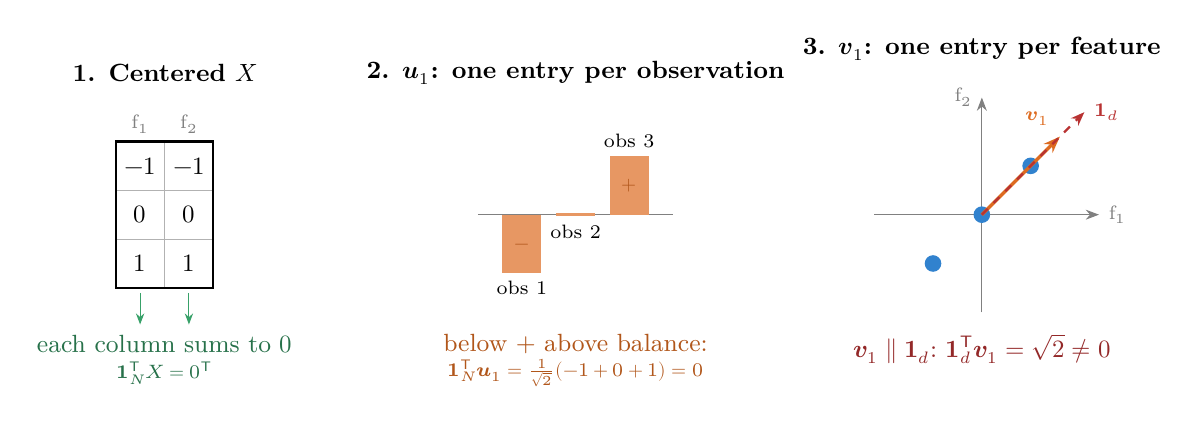
\begin{tikzpicture}[x=0.62cm,y=0.62cm, every node/.style={font=\small}]
  % ---- panel 1: the matrix with column sums
  \begin{scope}
    \node at (1,4.4) {\textbf{1. Centered $X$}};
    \foreach \r/\a/\b in {0/1/1,1/0/0,2/-1/-1} {
      \draw[gray!60] (0,\r) rectangle (1,\r+1); \draw[gray!60] (1,\r) rectangle (2,\r+1);
      \node at (0.5,\r+0.5) {$\a$}; \node at (1.5,\r+0.5) {$\b$};
    }
    \draw[thick] (0,0) rectangle (2,3);
    \node[gray, font=\scriptsize] at (0.5,3.35) {f$_1$}; \node[gray, font=\scriptsize] at (1.5,3.35) {f$_2$};
    \foreach \c in {0.5,1.5} \draw[-{Stealth[length=4pt]}, accentD] (\c,-0.1) -- (\c,-0.75);
    \node[accentD!70!black] at (1,-1.15) {each column sums to $0$};
    \node[accentD!70!black, font=\scriptsize] at (1,-1.75) {$\one_N\T X=\bm0\T$};
  \end{scope}
  % ---- panel 2: u1 as a bar chart over observations
  \begin{scope}[xshift=4.6cm]
    \node at (2,4.4) {\textbf{2. $\vu_1$: one entry per observation}};
    \draw[gray] (0,1.5) -- (4,1.5);
    \fill[accentC!70] (0.5,1.5) rectangle (1.3,0.3);
    \fill[accentC!70] (1.6,1.47) rectangle (2.4,1.53);
    \fill[accentC!70] (2.7,1.5) rectangle (3.5,2.7);
    \node[font=\scriptsize] at (0.9,0.0) {obs 1}; \node[font=\scriptsize] at (2.0,1.15) {obs 2}; \node[font=\scriptsize] at (3.1,3.0) {obs 3};
    \node[font=\scriptsize, accentC!80!black] at (0.9,0.85) {$-$}; \node[font=\scriptsize, accentC!80!black] at (3.1,2.1) {$+$};
    \node[accentC!80!black] at (2,-1.15) {below + above balance:};
    \node[accentC!80!black, font=\scriptsize] at (2,-1.75) {$\one_N\T\vu_1=\tfrac1{\sqrt2}(-1+0+1)=0$};
  \end{scope}
  % ---- panel 3: feature space with v1 parallel to 1_d
  \begin{scope}[xshift=11.0cm, yshift=1.5*0.62cm]
    \node at (0,3.4) {\textbf{3. $\vv_1$: one entry per feature}};
    \draw[-{Stealth}, gray] (-2.2,0) -- (2.4,0) node[right, font=\scriptsize] {f$_1$};
    \draw[-{Stealth}, gray] (0,-2.0) -- (0,2.4) node[left, font=\scriptsize] {f$_2$};
    \foreach \p in {(-1,-1),(0,0),(1,1)} \fill[dataC] \p circle (3pt);
    \draw[-{Stealth[length=6pt]}, very thick, accentC] (0,0) -- (1.6,1.6) node[above left, font=\scriptsize] {$\vv_1$};
    \draw[-{Stealth[length=5pt]}, thick, dashed, thmred] (0,0) -- (2.1,2.1) node[right, font=\scriptsize] {$\one_d$};
    \node[thmred!80!black] at (0,-2.75) {$\vv_1\parallel\one_d$:\ $\one_d\T\vv_1=\sqrt2\ne0$};
  \end{scope}
\end{tikzpicture}
\caption{Why centering constrains $\vu$ but not $\vv$. Centering is a statement about \textbf{columns} summing over
\textbf{observations} (panel 1). $\vu_1$ is indexed by observations, so its entries must balance around $0$ (panel 2). $\vv_1$
is indexed by features and here points exactly along $\one_d=(1,1)$ (panel 3): the data vary in the direction where both
features rise together, and nothing forbids a PC from adding features with positive weights.}
\end{figure}

\begin{careful}
Two easy confusions. (1) Centering says ``each \emph{feature's} values across observations sum to $0$'', not ``a PC's feature
weights sum to $0$''. So PC1 $=\tfrac1{\sqrt2}(\text{feature 1})+\tfrac1{\sqrt2}(\text{feature 2})$ is perfectly allowed. (2) In the \emph{full} SVD, the
extra left singular vectors with $\sigma=0$ fill out the rest of $\R^N$, and $\one_N/\sqrt N$ is in their span (Fact~\ref{kf:toolbox}: $\one_N\in\ker X\T$).
The right singular vectors would be $\perp\one_d$ only if every \emph{row} summed to $0$ (each observation's features
cancelling), which is a different and unusual kind of centering.
\end{careful}

\begin{proposition}{Kept part $\perp$ discarded part}{keptdisc}
Let $V_k=[\vv_1\cdots\vv_k]$. Every centered sample splits uniquely into two perpendicular pieces:
\[
\vx_i\T=\underbrace{\vx_i\T V_kV_k\T}_{\text{kept: in }\spn(\vv_1,\dots,\vv_k)}+\underbrace{\vx_i\T(I-V_kV_k\T)}_{\text{discarded: in }\spn(\vv_{k+1},\dots,\vv_r)} ,
\]
and the row space of $X$ is the orthogonal direct sum $\spn(\vv_1,\dots,\vv_k)\oplus\spn(\vv_{k+1},\dots,\vv_r)$.
\end{proposition}
\begin{proofsketch}
$V_kV_k\T$ is the orthogonal projector onto the kept span, and $I-V_kV_k\T$ projects onto its
orthogonal complement. The $\vv_j$ are orthonormal, so every discarded direction is perpendicular to
every kept one. Each row of $X$ lies in $\spn(\vv_1,\dots,\vv_r)$, so the residual lands in the discarded span.
\end{proofsketch}

\textbf{Compression as encode/decode.} Keeping $k$ components gives
$X\approx U_k\Sigma_kV_k\T$ with shapes $(N\times k)(k\times k)(k\times d)$. The \textbf{encoder} is
$\vx\mapsto V_k\T\vx$ ($d$ numbers $\to$ $k$ numbers). The compressed data set is $U_k\Sigma_k$, and the
\textbf{decoder} $V_k\T$ maps the $k$ numbers back to $\R^d$. The decoded point is the kept piece above,
and its error is the discarded piece.

\subsection{Truncated SVD: low-rank approximation without centering}

Lecture~6 put the two pictures side by side:
\[
\begin{bmatrix}\vx_1\T-\xbar\T\\\vdots\\\vx_N\T-\xbar\T\end{bmatrix}
=\big[\,\vy_1\cdots\vy_k\ \vy_{k+1}\cdots\vy_d\,\big]\begin{bmatrix}\vw_1\T\\\vdots\\\vw_d\T\end{bmatrix}
\ \Rightarrow\ \vx_i\T-\xbar\T\approx(y_{i1},\dots,y_{ik})\begin{bmatrix}\vw_1\T\\\vdots\\\vw_k\T\end{bmatrix}
\quad\text{(PCA, centered)}
\]
\[
\begin{bmatrix}\vx_1\T\\\vdots\\\vx_N\T\end{bmatrix}
=\big[\vu_1\cdots\vu_k\ \vu_{k+1}\cdots\big]
\begin{bmatrix}\sigma_1&&\\&\ddots&\\&&\ddots\end{bmatrix}
\begin{bmatrix}\vv_1\T\\\vdots\end{bmatrix}
\ \Rightarrow\ \vx_i\T\approx(u_{i1}\sigma_1,\dots,u_{ik}\sigma_k)\begin{bmatrix}\vv_1\T\\\vdots\\\vv_k\T\end{bmatrix}
\quad\text{(SVD, not centered)}
\]

\begin{proposition}{Frobenius norm from singular values}{frosvd}
For any $A\in\R^{N\times d}$ with SVD $A=U\Sigma V\T$,
\[
\Fro{A}=\sqrt{\tr(A\T A)}=\sqrt{\tr(V\Sigma\T\Sigma V\T)}=\sqrt{\tr(V\T V\,\Sigma\T\Sigma)}
=\sqrt{\tr(\Sigma\T\Sigma)}=\sqrt{\textstyle\sum_{i=1}^{\min(N,d)}\sigma_i^2}.
\]
\end{proposition}
\begin{proofsketch}
$\Fro{A}^2=\sum_{i,j}A_{ij}^2$ is the sum of the squared lengths of the columns, and
$(A\T A)_{jj}=\norm{\text{column } j}^2$, so $\Fro{A}^2=\tr(A\T A)$. Next,
$A\T A=V\Sigma\T U\T U\Sigma V\T=V\Sigma\T\Sigma V\T$ because $U\T U=I$. The trace is cyclic
($\tr(PQ)=\tr(QP)$), so we can move $V$ to the front, and then $V\T V=I$ drops out. Finally,
$\Sigma\T\Sigma=\diag(\sigma_1^2,\dots,\sigma_{\min(N,d)}^2)$ (padded with zeros), and its
trace is the sum of the $\sigma_i^2$.
\end{proofsketch}

\begin{intuition}
Rotations do not change lengths, so they do not change the Frobenius norm either. The SVD
peels off the two rotations $U$ and $V$, and what is left is the ``pure stretch''
$\Sigma$. So the total squared size of a matrix equals the total squared stretch,
$\sum\sigma_i^2$. This is the matrix version of ``total variation is preserved by a
rotation'' from Theorem~\ref{thm:scores}.
\end{intuition}

\begin{theorem}{Eckart--Young}{eckart}
Let $A=\sum_{i}\sigma_i\vu_i\vv_i\T$ with $\sigma_1\ge\sigma_2\ge\cdots$ (sum up to
$\min(N,d)$; the board writes $d$, which assumes $N\ge d$). The truncation
$A_k=\sum_{i\le k}\sigma_i\vu_i\vv_i\T$ is the best rank-$k$ approximation of $A$ in
Frobenius norm:
\[
\min_{\substack{B\in\R^{N\times d}\\ \rank(B)\le k}}\Fro{A-B}^2=\Fro{A-A_k}^2=\sigma_{k+1}^2+\cdots+\sigma_{\min(N,d)}^2 .
\]
\end{theorem}
\begin{proofsketch}
\emph{The truncation achieves this value.} $A-A_k=\sum_{i>k}\sigma_i\vu_i\vv_i\T$. This is
itself an SVD (same orthonormal $\vu$'s and $\vv$'s, singular values
$\sigma_{k+1},\sigma_{k+2},\dots$), so Prop.~\ref{prop:frosvd} gives
$\Fro{A-A_k}^2=\sum_{i>k}\sigma_i^2$.
\emph{Nothing does better.} This is the content of the theorem. One standard argument
applies the PCA optimality theorem (Theorem~\ref{thm:bestsub}) to the rows of $A$. Its
proof works for any matrix $\tfrac1N\sum_i\vx_i\vx_i\T$, centered or not, so use
$\tfrac1N A\T A$ in place of $\Sig$. The
rows of a rank-$k$ matrix $B$ lie in some $k$-dimensional subspace $V$. The best $B$ with
rows in $V$ projects each row onto $V$, and the best $V$ is spanned by the top right
singular vectors, which leaves exactly $\sum_{i>k}\sigma_i^2$.
\end{proofsketch}

\begin{deeper}
\textbf{Two supporting facts, and a second proof.}
(1) Why the norm of $\sum_{i>k}\sigma_i\vu_i\vv_i\T$ is $\sum_{i>k}\sigma_i^2$ without any SVD reasoning: the rank-one
matrices $\vu_i\vv_i\T$ are \emph{orthonormal} under the Frobenius inner product
$\langle P,Q\rangle_F=\tr(P\T Q)$, because
$\langle\vu_i\vv_i\T,\vu_j\vv_j\T\rangle_F=(\vu_i\T\vu_j)(\vv_i\T\vv_j)$, which is $1$ if $i=j$ and $0$ otherwise.
The squared norm of a sum of orthonormal pieces is the sum of the squared coefficients (Pythagoras).
(2) \emph{Weyl's inequality} for singular values says $\sigma_{i+j-1}(P+Q)\le\sigma_i(P)+\sigma_j(Q)$ (we take it as given).
Apply it with $P=A-B$, $Q=B$ and $j=k+1$. Since $\rank B\le k$, $\sigma_{k+1}(B)=0$, so
$\sigma_{i+k}(A)\le\sigma_i(A-B)$ for every $i$. Squaring and summing,
$\Fro{A-B}^2=\sum_i\sigma_i(A-B)^2\ge\sum_i\sigma_{i+k}(A)^2=\sum_{j>k}\sigma_j^2$.
In words: a rank-$k$ matrix can ``absorb'' at most the top $k$ singular values, and
everything below is left over.
\end{deeper}

\subsubsection*{Reading $A_k$ as a projection}

\begin{proposition}{The best rank-$k$ approximation is a projection}{akproj}
Let $U_k=[\vu_1\cdots\vu_k]$ and $V_k=[\vv_1\cdots\vv_k]$. Then
\[
A_k=U_kU_k\T A=A\,V_kV_k\T .
\]
$U_kU_k\T$ is the orthogonal projector onto $\spn(\vu_1,\dots,\vu_k)$: for any $\bm y\in\R^N$,
\[
U_kU_k\T\bm y=\sum_{j=1}^k(\vu_j\T\bm y)\,\vu_j ,
\]
the piece of $\bm y$ lying in that span. So $A_k$ is $A$ with every \emph{column} projected onto the top $k$ left singular vectors,
or equivalently with every \emph{row} projected onto the top $k$ right singular vectors.
\end{proposition}
\begin{proofsketch}
\emph{Why $U_kU_k\T\bm y$ is a projection.} Do it in two steps.
\begin{enumerate}[nosep,label=\arabic*)]
\item $U_k\T\bm y=(\vu_1\T\bm y,\dots,\vu_k\T\bm y)$. The $\vu_j$ are unit vectors and mutually perpendicular, so each entry is just ``how much
of $\bm y$ points along $\vu_j$''.
\item $U_k(\cdot)$ multiplies each $\vu_j$ by its amount and adds them up, giving $\sum_j(\vu_j\T\bm y)\vu_j$.
\end{enumerate}
What is left over, $\bm y-U_kU_k\T\bm y$, has dot product $\vu_i\T\bm y-\vu_i\T\bm y=0$ with every $\vu_i$ ($i\le k$), so it is
perpendicular to the span: everything perpendicular gets dropped, and nothing in the span is lost.

\emph{Why this gives $A_k$.} From $A=U\Sigma V\T$ and $U\T U=I$, we get $U\T A=\Sigma V\T$; keeping the first $k$ rows,
$U_k\T A=\Sigma_kV_k\T$. Hence $U_kU_k\T A=U_k\Sigma_kV_k\T=A_k$. The same argument with $AV=U\Sigma$ gives $AV_k=U_k\Sigma_k$ and
$AV_kV_k\T=A_k$.
\end{proofsketch}

\begin{example}{Projecting onto one direction}{projone}
In $\R^3$ take $\vu_1=\tfrac1{\sqrt2}(1,1,0)$ and $\bm y=(3,1,5)$. Then $\vu_1\T\bm y=\tfrac4{\sqrt2}$, and
$U_1U_1\T\bm y=\tfrac4{\sqrt2}\cdot\tfrac1{\sqrt2}(1,1,0)=(2,2,0)$. The dropped part is $(1,-1,5)$, and $(1,-1,5)\cdot(1,1,0)=0$, as it should be.
\end{example}

\textbf{The general formula.} If $Z\in\R^{N\times k}$ has independent columns that are \emph{not} orthonormal, the projector onto
their span is
\[
P_Z=Z(Z\T Z)^{-1}Z\T .
\]
$Z\T\bm y$ still computes the dot products with the columns, but when the columns overlap or have different lengths those dot
products are no longer the right amounts, and $(Z\T Z)^{-1}$ corrects them. (This is the least-squares fit of $\bm y$ on the columns of
$Z$: the coefficients $(Z\T Z)^{-1}Z\T\bm y$ solve the normal equations.) When the columns are orthonormal, $Z\T Z=I$, the inverse disappears, and
$P_Z$ collapses to $ZZ\T$, which is $U_kU_k\T$ above.

\begin{careful}
\textbf{$ZZ\T$ is \emph{not} a projector unless the columns are orthonormal.} Take $\bm z_1=(1,0,0)$, $\bm z_2=(1,1,0)$, which span the $xy$-plane,
and $\bm y=(0,1,0)$, which already lies in it. Then $Z\T\bm y=(0,1)$ and $ZZ\T\bm y=(1,1,0)\ne\bm y$: wrong. With the correction,
$Z\T Z=\begin{bmatrix}1&1\\1&2\end{bmatrix}$, $(Z\T Z)^{-1}=\begin{bmatrix}2&-1\\-1&1\end{bmatrix}$, so the coefficients are $(Z\T Z)^{-1}(0,1)=(-1,1)$ and
$P_Z\bm y=-\bm z_1+\bm z_2=(0,1,0)=\bm y$. Every orthogonal projector $P$ satisfies $P^2=P$ (projecting twice changes nothing) and
$P\T=P$; the matrix $ZZ\T$ here fails the first: $(ZZ\T)^2\ne ZZ\T$.
\end{careful}

\begin{intuition}
Seeing $A_k$ as $U_kU_k\T A$ says what the truncated SVD \emph{does}: it keeps the part of the data lying in the best $k$-dimensional
subspace and throws the rest away. Eckart--Young then says this subspace is the best one to project onto, and the thrown-away part
has squared size $\sigma_{k+1}^2+\cdots$.
\end{intuition}

\begin{intuition}
Both pictures say the same thing: \emph{learn $W,H$ such that $X\approx WH$} with a thin
middle dimension $k$. PCA/SVD put no constraint on the signs of $W$ and $H$ and measure
error in squared Frobenius norm. Changing the constraints and the error measure gives a
whole family of methods. The next one is NMF.
\end{intuition}

% ==================================================================
\section{Nonnegative Matrix Factorization (NMF)}
% ==================================================================

\subsection{The model}

\begin{definition}{NMF}{nmf}
Given a nonnegative data matrix $X\in\R_{\ge0}^{N\times d}$ and a rank $k$, find
\[
X\approx WH,\qquad W\in\R_{\ge0}^{N\times k},\quad H\in\R_{\ge0}^{k\times d}.
\]
Row-wise: $\vx_i\T\approx\sum_{j=1}^k W_{ij}\,\vh_j\T$, so each sample is a
\emph{nonnegative} combination of $k$ nonnegative ``parts'' $\vh_1,\dots,\vh_k$ (the rows of $H$).
\end{definition}

\begin{proposition}{A perfect factorization caps the rank}{nmfrank}
If $X=WH$ exactly with $k$ parts, then $\rank(X)\le k$. Equality is \emph{not} guaranteed.
\end{proposition}
\begin{proofsketch}
Every row $\vx_i\T=\sum_jW_{ij}\vh_j\T$ lies in $\spn\{\vh_1,\dots,\vh_k\}$, and a span of $k$ vectors has
at most $k$ independent directions. The parts can be redundant, though. With $k=3$ and
$\vh_1=(1,0)$, $\vh_2=(0,1)$, $\vh_3=(1,1)=\vh_1+\vh_2$, any $X=WH$ has rank at most $2<3$.
\end{proofsketch}

\begin{intuition}
$k$ is the number of component \emph{slots} you allow, usually much smaller than $N$ and $d$.
When $k<\rank X$ (the usual compression setting) no factorization is exact, and $X\approx WH$ is a
genuine approximation. A perfect fit needs at least $\rank X$ slots, and for NMF possibly
\emph{more}. The smallest $k$ admitting an exact \emph{nonnegative} factorization is the
\textbf{nonnegative rank}, and $\rank(X)\le\operatorname{rank}_+(X)$. Nonnegativity can force extra parts
even when the ordinary rank is small. This is the exact-fit version of the gap in
Theorem~\ref{thm:nmffloor}.
\end{intuition}

\begin{definition}{Nonnegative rank}{nnrank}
For $X\in\R^{N\times d}_{\ge0}$, the \textbf{nonnegative rank} $\operatorname{rank}_+(X)$ is the smallest $k$ for which an
\emph{exact} factorization $X=WH$ exists with $W\in\R^{N\times k}_{\ge0}$ and $H\in\R^{k\times d}_{\ge0}$.
\end{definition}

\begin{theorem}{Sandwich for the nonnegative rank}{nnsandwich}
For every $X\in\R^{N\times d}_{\ge0}$,
\[
\rank(X)\ \le\ \operatorname{rank}_+(X)\ \le\ \min\{N,d\}.
\]
\end{theorem}
\begin{proofsketch}
\emph{Upper bound (by construction).} Two explicit nonnegative factorizations always exist:
\[
X=\underbrace{I_N}_{N\times N}\,\underbrace{X}_{N\times d}\quad(k=N),
\qquad
X=\underbrace{X}_{N\times d}\,\underbrace{I_d}_{d\times d}\quad(k=d).
\]
Both are legal for NMF because $X\ge0$ by assumption and the identity matrix has only $0$s and
$1$s. Since $\operatorname{rank}_+(X)$ is the \emph{smallest} workable $k$, it is at most any $k$ that works,
so $\operatorname{rank}_+(X)\le N$ and $\operatorname{rank}_+(X)\le d$, i.e.\ $\operatorname{rank}_+(X)\le\min\{N,d\}$.

\emph{Lower bound (for every factorization).} Take any exact factorization $X=WH$ with inner
dimension $k$, nonnegative or not. Then
$\rank(X)=\rank(WH)\le\min\{\rank W,\rank H\}\le k$ (Prop.~\ref{prop:nmfrank}). This holds for
\emph{every} factorization, so in particular for an optimal nonnegative one, whose inner dimension
is $k^\star=\operatorname{rank}_+(X)$. Hence $\rank(X)\le\operatorname{rank}_+(X)$. Nonnegativity is used only to say
which $k$ we plug in.
\end{proofsketch}

\begin{careful}
\textbf{Which way does each argument point? (Bounding a minimum.)} Rank facts such as
$\rank(W)\le\min\{N,k\}$ and $\rank(H)\le\min\{k,d\}$ combine to give $k\ge\rank(X)$, a statement of the form
``$k$ is \emph{at least} something''. No chain of such inequalities can ever produce an \emph{upper}
bound on $\operatorname{rank}_+(X)$. The logical shape of the two directions differs:
\begin{itemize}[nosep]
\item $\min\le c$ is an \textbf{existence} claim: exhibit one feasible $k\le c$ (here, the identity factorization);
\item $\min\ge c$ is a \textbf{for-all} claim: show every $k<c$ is impossible (here, the rank argument).
\end{itemize}
Rule of thumb: an upper bound on a minimum (or a lower bound on a maximum) usually means
``find an example''. The other direction means ``prove nothing better is possible''. The words
``bounded above'' plus a definition of the form ``the smallest $k$ such that\dots'' signal the first kind.
\end{careful}

\begin{example}{The construction need not be optimal}{nnwasteful}
$X=\begin{bmatrix}1&1\\1&1\end{bmatrix}$ has $\rank X=1$. The factorization $X=I_2\cdot X$ uses $k=2$. It is valid but
wasteful, because $X=\begin{bmatrix}1\\1\end{bmatrix}\begin{bmatrix}1&1\end{bmatrix}$ uses $k=1$, so here
$\operatorname{rank}_+(X)=\rank(X)=1$. Writing $W=I_N$ does \emph{not} say $X$ has rank $N$. It only shows
that inner dimension $N$ is enough. The upper-bound proof needs some valid factorization, not the best one.
\end{example}

\begin{center}
\renewcommand{\arraystretch}{1.35}
\small
\begin{tabular}{@{}>{\raggedright\arraybackslash}p{4.6cm}>{\raggedright\arraybackslash}p{9.2cm}@{}}
\toprule
situation & what you can say about $k$ \\
\midrule
any exact factorization $X=WH$ (signs unrestricted) & $\rank(X)\le k$ \\
exact NMF, $X=WH$ with $W,H\ge0$ & $\rank(X)\le k$ (the same fact; nonnegativity is not used) \\
smallest exact NMF & $k=\operatorname{rank}_+(X)$, and $\rank(X)\le\operatorname{rank}_+(X)\le\min\{N,d\}$ \\
approximate NMF, $X\approx WH$ & $k$ is a \emph{choice}, often deliberately $k<\rank(X)$ for compression, so exact equality is impossible \\
\bottomrule
\end{tabular}
\end{center}

\begin{example}{Nonnegativity can cost an extra component}{nnstrict}
Sometimes $\operatorname{rank}_+(X)=\rank(X)$ (Example~\ref{ex:nnwasteful}: both are $1$), and sometimes the inequality is strict. A standard example is
\[
X=\begin{bmatrix}1&1&0&0\\1&0&1&0\\0&1&0&1\\0&0&1&1\end{bmatrix}.
\]
Rows $1+4$ and $2+3$ both equal $(1,1,1,1)$, so the rows are dependent and $\rank X=3$ (row reduction confirms
three pivots). Yet its nonnegative rank is known to be $4$. Every factorization with three parts needs
some negative entries. (This matrix measures, for each corner of a square, its distance to each edge, and the
gap $3<4$ is a classical fact about the square.)
\end{example}

\begin{intuition}
\textbf{Why nonnegativity can need more parts: no cancellation.} With signs allowed, a part may contain
something ``too much'' and another part can subtract it away. That is how SVD builds $X$ from only
$\rank X$ pieces. NMF parts can only be \emph{added}, so every part must already fit inside every sample that
uses it. If the data's shape does not allow such purely additive building blocks, you need extra parts.
The cone picture says the same: the $k$ parts must span a cone that contains all the data, and a
cone with only $\rank X$ edges may be too narrow to hold it.
\end{intuition}

\begin{intuition}
Think of each $k=1,2,3,\dots$ as getting a ``yes'' or ``no'' to the question ``does an exact nonnegative factorization
with $k$ parts exist?'' Every $k<\rank X$ gets ``no'' (not enough independent building blocks), and
$k=\min\{N,d\}$ gets ``yes'' (the identity trick). Once some $k$ works, every larger $k$ works too (pad
$W$ with a zero column and $H$ with a zero row). So the ``yes'' answers form a range
$\{\operatorname{rank}_+(X),\dots\}$ whose start lies between $\rank(X)$ and $\min\{N,d\}$.
\end{intuition}

\begin{intuition}
Picture $16\times16$ images flattened to vectors in $\R^{256}$. Pixel intensities are
$\ge0$. Because NMF can only \emph{add} parts, never subtract them, the rows of $H$ tend to be
localised pieces such as strokes or facial features. PCA loadings mix signs, so they
come out as ``ghostly'' global patterns that cancel each other.
\end{intuition}

\subsection{How to measure the quality of the approximation}

Three standard losses, all written entrywise over $s=1..N$, $t=1..d$:
\begin{align*}
\text{Frobenius norm:}\quad & \Fro{X-WH}^2=\sum_{s,t}\big(X_{st}-(WH)_{st}\big)^2\\
\text{KL divergence:}\quad & D_{KL}(X\,\|\,WH)=\sum_{s,t}\Big[X_{st}\log\frac{X_{st}}{(WH)_{st}}-X_{st}+(WH)_{st}\Big]\\
\text{Itakura--Saito divergence:}\quad & D_{IS}(X\,\|\,WH)=\sum_{s,t}\Big[\frac{X_{st}}{(WH)_{st}}-\log\frac{X_{st}}{(WH)_{st}}-1\Big]
\end{align*}

\begin{center}
\renewcommand{\arraystretch}{1.3}
\begin{tabular}{lccc}
\toprule
Loss & Sensitive to scale? & Sensitive to outliers? & Likelihood model \\
\midrule
Frobenius & Yes & Yes & Gaussian noise \\
KL divergence & Less so & Yes (less so) & Poisson counts \\
IS divergence & \textbf{No} & Yes (even less so) & multiplicative Gamma noise\\
\bottomrule
\end{tabular}
\end{center}

\begin{deeper}
Why does the scale sensitivity go down the table? Scale both arguments by $c>0$:
$\Fro{cX-cY}^2=c^2\Fro{X-Y}^2$, $D_{KL}(cX\|cY)=c\,D_{KL}(X\|Y)$, and
$D_{IS}(cX\|cY)=D_{IS}(X\|Y)$. Large entries dominate the Frobenius loss
quadratically, dominate KL only linearly, and do not dominate IS at all.

The lecture asked: maximum likelihood? generative models? Each loss is a negative
log-likelihood. Minimizing Frobenius is MLE under $X_{st}\sim\mathcal N((WH)_{st},\sigma^2)$.
Minimizing KL is MLE under $X_{st}\sim\text{Poisson}((WH)_{st})$, natural for count data.
Minimizing IS is MLE under multiplicative noise $X_{st}=(WH)_{st}\cdot\varepsilon$ with
$\varepsilon\sim\text{Gamma}$, natural for power spectra in audio. Picking a loss amounts to
picking a noise model.
\end{deeper}

\subsection{Geometry: the simplicial cone}

\begin{definition}{Simplicial cone (positive span)}{cone}
The positive span of $\vh_1,\dots,\vh_k\in\R^d$ is
\[
\cone\{\vh_1,\dots,\vh_k\}=\Big\{\bm v\in\R^d:\ \bm v=\sum_{j=1}^k a_j\vh_j,\ a_1,\dots,a_k\ge0\Big\}.
\]
\end{definition}

In a \emph{perfect} NMF $X=WH$ we have $\vx_i=\sum_j W_{ij}\vh_j$ with $W_{ij}\ge0$, so
\textbf{every data point lies in the positive span of $\vh_1,\dots,\vh_k$}. In $\R^3$
with $k=2$, the data must lie in the wedge between $\vh_1$ and $\vh_2$.

\begin{figure}[htbp]
\centering
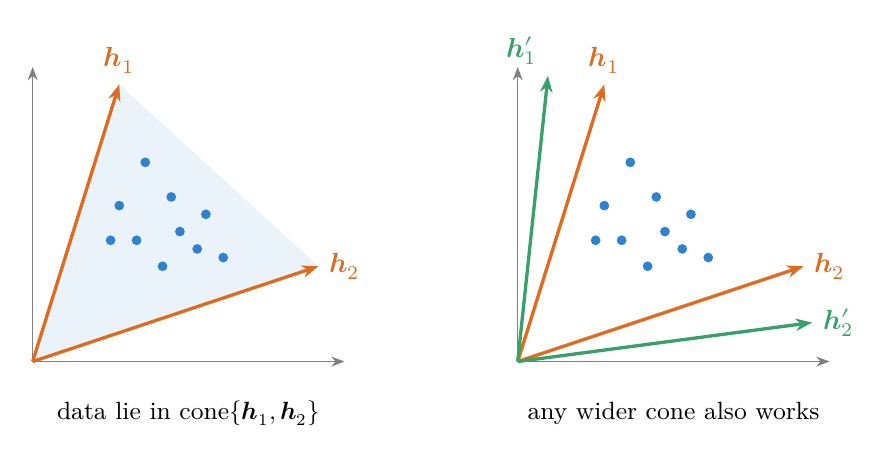
\begin{tikzpicture}[scale=1.1]
\begin{scope}
  \draw[-{Stealth}, gray] (0,0) -- (3.6,0);
  \draw[-{Stealth}, gray] (0,0) -- (0,3.4);
  \fill[dataC!10] (0,0) -- (3.3,1.1) -- (1.0,3.2) -- cycle;
  \draw[-{Stealth[length=6pt]}, very thick, accentC] (0,0) -- (3.3,1.1) node[right] {$\vh_2$};
  \draw[-{Stealth[length=6pt]}, very thick, accentC] (0,0) -- (1.0,3.2) node[above] {$\vh_1$};
  \foreach \x/\y in {1.2/1.4,1.5/1.1,1.0/1.8,1.9/1.3,1.6/1.9,2.2/1.2,1.3/2.3,2.0/1.7,0.9/1.4,1.7/1.5}
    \fill[dataC] (\x,\y) circle (1.6pt);
  \node[font=\small, align=center] at (1.8,-0.6) {data lie in $\cone\{\vh_1,\vh_2\}$};
\end{scope}
\begin{scope}[xshift=5.6cm]
  \draw[-{Stealth}, gray] (0,0) -- (3.6,0);
  \draw[-{Stealth}, gray] (0,0) -- (0,3.4);
  \foreach \x/\y in {1.2/1.4,1.5/1.1,1.0/1.8,1.9/1.3,1.6/1.9,2.2/1.2,1.3/2.3,2.0/1.7,0.9/1.4,1.7/1.5}
    \fill[dataC] (\x,\y) circle (1.6pt);
  \draw[-{Stealth[length=6pt]}, very thick, accentC] (0,0) -- (3.3,1.1) node[right] {$\vh_2$};
  \draw[-{Stealth[length=6pt]}, very thick, accentC] (0,0) -- (1.0,3.2) node[above] {$\vh_1$};
  \draw[-{Stealth[length=6pt]}, very thick, accentD] (0,0) -- (3.4,0.45) node[right] {$\vh_2'$};
  \draw[-{Stealth[length=6pt]}, very thick, accentD] (0,0) -- (0.35,3.3) node[above left] {$\vh_1'$};
  \node[font=\small, align=center] at (1.8,-0.6) {any wider cone also works};
\end{scope}
\end{tikzpicture}
\caption{The NMF cone, and why it is not unique. Any pair of nonnegative vectors whose
cone contains the data reproduces it exactly, so there are infinitely many valid
$(\vh_1,\vh_2)$.}
\end{figure}

\subsection{Non-uniqueness and estimation}

\begin{theorem}{NMF solutions are not unique}{nonunique}
Whatever measure of approximation quality you use (Frobenius, KL, IS), the optimal $W,H$ are
\textbf{not unique}, and the problem is a \textbf{non-convex optimization}.
\end{theorem}

\begin{intuition}
There are three sources of ambiguity: (i) the cone picture above, (ii) rescaling,
$WH=(WD)(D^{-1}H)$ for any positive diagonal $D$, and (iii) relabelling the $k$ parts by
a permutation. Even with $W$ fixed the loss is convex in $H$ (and vice versa). It is not
convex in the pair $(W,H)$ jointly, so there can be many local minima.
\end{intuition}

\subsubsection*{What is wrong with a huge $W$ and a tiny $H$?}

For the reconstruction alone, \textbf{nothing}. Since
\[
WH=(100W)(0.01H),
\]
the predicted matrix $WH$, the Poisson rates and the KL data-fit loss are exactly unchanged. The
problem is that the individual factors become arbitrary. Is a part ``very active'' because $W$ is
huge, or is it weakly defined in $H$ with a huge compensating $W$? From $WH$ alone you cannot
tell. This is \textbf{scale ambiguity}, source (ii) above. Huge--tiny factors are also inconvenient:
\begin{itemize}[nosep]
\item they are harder to interpret;
\item numerical updates can become unstable or poorly scaled;
\item once you add noise, constraints or regularization, the two factorizations no longer behave equivalently.
\end{itemize}

A \textbf{ridge penalty} picks a preference among equally good products:
\[
\frac{\lambda}{2}\Big(\Fro{W}^2+\Fro{H}^2\Big).
\]
For the same product it dislikes $(100W,\,0.01H)$, because $100W$ has a gigantic squared norm. It
prefers the scaling where neither factor is unnecessarily extreme. Concretely, over the rescalings
$(cW,\,H/c)$ the penalty is $c^2\Fro{W}^2+c^{-2}\Fro{H}^2$, which is minimized at
$c^2=\Fro{H}/\Fro{W}$, i.e.\ exactly where $\Fro{cW}=\Fro{H/c}$: the two factors are balanced.

\begin{intuition}
Ridge does not say ``a large $W$ is intrinsically bad''. It says: \emph{if two pairs $(W,H)$
predict the same $WH$, choose the well-scaled one.}
\end{intuition}

\textbf{Estimating NMF in practice.}
\begin{enumerate}[nosep]
\item There is \textbf{no closed-form expression} for the optimal $W,H$, unlike the SVD.
\item So run iterative descent from \textbf{several different initializations} and keep the best result.
\end{enumerate}

\begin{figure}[htbp]
\centering
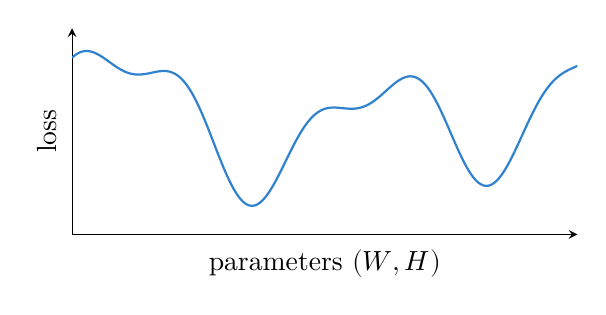
\begin{tikzpicture}
\begin{axis}[width=8cm, height=4.2cm, axis lines=left, xtick=\empty, ytick=\empty, xlabel={parameters $(W,H)$}, ylabel={loss}, ymin=-0.3, ymax=3.2]
\addplot[thick, dataC, domain=0:10, samples=200] {1.4+0.9*sin(deg(1.3*x))+0.12*(x-5)^2*0.3+0.4*cos(deg(2.7*x))};
\end{axis}
\end{tikzpicture}
\caption{A non-convex loss landscape. Different starting points descend into different
local minima, which is why we try several initializations.}
\end{figure}

\subsection{Gradients of the KL loss}

Write $(WH)_{st}=\sum_{p=1}^k W_{sp}H_{pt}$. Then
\[
\frac{\partial (WH)_{st}}{\partial W_{ij}}=\begin{cases}H_{jt}&s=i\\0&s\ne i\end{cases},
\qquad
\frac{\partial (WH)_{st}}{\partial H_{ij}}=\begin{cases}W_{si}&t=j\\0&t\ne j\end{cases}.
\]
Differentiating $D_{KL}$ term by term (the $X\log X-X$ parts do not depend on $W,H$):
\[
\frac{\partial D}{\partial W_{ij}}=\sum_{s,t}\Big[-X_{st}\frac{1}{(WH)_{st}}+1\Big]\frac{\partial(WH)_{st}}{\partial W_{ij}}
=\sum_{t=1}^d\Big(1-\frac{X_{it}}{(WH)_{it}}\Big)H_{jt},
\]
\[
\frac{\partial D}{\partial H_{ij}}=\sum_{s=1}^N\Big(1-\frac{X_{sj}}{(WH)_{sj}}\Big)W_{si}.
\]

\subsubsection*{Why the double sum collapses to a single sum}

The loss sums over \emph{every} entry $(s,t)$, but the gradient for $W_{ij}$ keeps only row $s=i$. Nothing
was dropped by choice: the other terms do not contain $W_{ij}$, so their derivatives are zero, exactly as
\[
\frac{\partial}{\partial x}\big(x^2+y^2+z^2\big)=2x+0+0 .
\]

\begin{example}{The smallest case, written out}{collapse}
Take $N=d=2$ and $k=1$, so $W=\begin{bmatrix}W_{11}\\W_{21}\end{bmatrix}$, $H=\begin{bmatrix}H_{11}&H_{12}\end{bmatrix}$ and
\[
WH=\begin{bmatrix}W_{11}H_{11}&W_{11}H_{12}\\W_{21}H_{11}&W_{21}H_{12}\end{bmatrix}.
\]
Let $f$ be any per-entry loss (for KL, IS or Frobenius, $f$ depends on $X_{st}$ and $Y=(WH)_{st}$). The double sum $\sum_{s=1}^2\sum_{t=1}^2$ is
just four terms:
\[
L=f\big(\underbrace{W_{11}H_{11}}_{(WH)_{11}}\big)+f\big(\underbrace{W_{11}H_{12}}_{(WH)_{12}}\big)+f\big(\underbrace{W_{21}H_{11}}_{(WH)_{21}}\big)+f\big(\underbrace{W_{21}H_{12}}_{(WH)_{22}}\big).
\]
By the chain rule,
\[
\frac{\partial L}{\partial W_{11}}=f'\big((WH)_{11}\big)H_{11}+f'\big((WH)_{12}\big)H_{12}+0+0
=\sum_{t=1}^{2}f'\big((WH)_{1t}\big)H_{1t}.
\]
The last two terms contain only $W_{21}$, so from $W_{11}$'s point of view they are constants. The sum over
\textbf{rows} collapses because $W_{11}$ lives only in row $1$ of $WH$. The sum over \textbf{columns} survives
because $W_{11}$ appears in every column of row $1$. (Symmetrically, $H_{1t}$ lives only in column $t$, so its
gradient keeps a sum over rows, as in $\partial D/\partial H_{ij}$ above.)
\end{example}

\begin{intuition}
\textbf{The indicator is bookkeeping.} Writing $\partial(WH)_{st}/\partial W_{ij}=\mathbf 1\{s=i\}H_{jt}$ keeps the double
sum on paper and says formally that every term from another row is zero. It does the same job as
``$+\,0+0$''. \textbf{Why fix one entry $W_{ij}$?} $W$ is not one variable but $N\times k$ separate numbers,
and ``the gradient with respect to $W$'' means one partial derivative for each. Computing
$\partial L/\partial W_{ij}$ for a \emph{general} $(i,j)$ produces all of them at once, just as one computes
$\partial/\partial x$, $\partial/\partial y$, $\partial/\partial z$ separately for $x^2+y^2+z^2$.
\end{intuition}

\subsection{From gradient descent to multiplicative updates}

\textbf{Iterative coordinate descent:} alternate descent steps over the entries of $W$ and of $H$.
With entrywise step sizes $\Delta^W_{ij},\Delta^H_{ij}>0$:
\begin{align*}
W_{ij}&\leftarrow W_{ij}-\Delta^W_{ij}\sum_t\Big(-\frac{X_{it}}{(WH)_{it}}+1\Big)H_{jt},\\
H_{ij}&\leftarrow H_{ij}-\Delta^H_{ij}\sum_s\Big(-\frac{X_{sj}}{(WH)_{sj}}+1\Big)W_{si}.
\end{align*}
\textbf{Problem:} a subtraction can push an entry below zero. Can we choose step sizes
that preserve the nonnegativity of the system?

\textbf{Trick (rescaled gradient descent):} choose
\[
\Delta^W_{ij}=\frac{W_{ij}}{\sum_t H_{jt}},\qquad \Delta^H_{ij}=\frac{H_{ij}}{\sum_s W_{si}} .
\]
Substituting, the $+\sum_tH_{jt}$ term cancels the leading $W_{ij}$:
\[
W_{ij}\leftarrow W_{ij}\,\frac{\sum_t H_{jt}\,X_{it}/(WH)_{it}}{\sum_t H_{jt}}\ \ \ge 0,
\qquad
H_{ij}\leftarrow H_{ij}\,\frac{\sum_s W_{si}\,X_{sj}/(WH)_{sj}}{\sum_s W_{si}}\ \ \ge0 .
\]
\textbf{Instead of subtracting, we get a multiplicative update.} Gradient descent, which
is a subtraction, becomes a multiplication.

\begin{theorem}{General multiplicative-update recipe (cheat-sheet)}{mu}
Split any gradient into nonnegative parts, $\frac{\partial f}{\partial W_{ij}}=\big(\tfrac{\partial f}{\partial W_{ij}}\big)^+-\big(\tfrac{\partial f}{\partial W_{ij}}\big)^-$,
and take the step $\Delta_{ij}=W_{ij}\big/\big(\tfrac{\partial f}{\partial W_{ij}}\big)^+$. Then
\[
W_{ij}\leftarrow W_{ij}-\frac{W_{ij}}{(\partial f)^+}\Big[(\partial f)^+-(\partial f)^-\Big]
= W_{ij}\,\frac{(\partial f/\partial W_{ij})^-}{(\partial f/\partial W_{ij})^+}.
\]
\end{theorem}

\begin{intuition}
The update multiplies by the ratio ``pull down / push up''. If the negative part of the
gradient wins, the entry grows. If the positive part wins, it shrinks. At a stationary
point the two parts balance, the ratio is $1$, and nothing moves. A zero entry stays
zero forever, which is why initializations must be strictly positive.
\end{intuition}

\subsubsection*{Is the split part of ordinary gradient descent? How would you know to do it?}

Write $P=(\partial f)^+$ and $N=(\partial f)^-$ for the two parts. The usual update does
\textbf{not} involve $P$ and $N$ at all. The general rule is
\[
W\leftarrow W-\eta\,\nabla_W L,
\]
where $\eta$ is a single number (the learning rate). The size of each step is $\eta$ times the
gradient, so it is large when the gradient is large and small near a minimum. This is what
backprop plus SGD does. Adam and other optimizers only change how $\eta$ and the gradient are combined.

Writing $\nabla_W L=P-N$ is \emph{not} part of the general rule. It is a rewrite of the same
gradient, done only for one specific trick: getting a multiplicative update. So
$W\leftarrow W-\eta(P-N)$ is still ordinary gradient descent with the gradient written in a
particular form. Nothing changes until you pick the special step size.

\textbf{Work backward from the goal.} A multiplicative update means
\[
W_{ia}\leftarrow W_{ia}\times(\text{something}\ge0),
\]
but gradient descent is subtractive: $W_{ia}-\eta_{ia}g_{ia}$. To turn that into a
multiplication, the step size has to cancel the leading $W_{ia}$. If $\eta_{ia}=W_{ia}/P_{ia}$ and
the gradient has the form $P_{ia}-N_{ia}$, then
\[
W_{ia}-\frac{W_{ia}}{P_{ia}}\big(P_{ia}-N_{ia}\big)=W_{ia}\,\frac{N_{ia}}{P_{ia}},
\]
and the subtraction disappears. The split is what makes this cancellation possible. For the result
to be nonnegative, $P$ and $N$ must both be nonnegative, so the natural move is to \textbf{sort the
gradient's terms by sign}: everything added goes in $P$, everything subtracted goes in $N$.

In practice this is a known template (Lee and Seung, 2001), not something you invent from
scratch. When a problem says ``choose step sizes to derive multiplicative updates'', it is pointing
at exactly this recipe (Theorem~\ref{thm:mu}):
\begin{enumerate}[nosep]
\item compute the gradient;
\item write it as (nonnegative terms) $-$ (nonnegative terms) $=P-N$;
\item set the per-entry step size $\eta=W\hdiv P$;
\item simplify to $W\leftarrow W\had N\hdiv P$.
\end{enumerate}

\begin{deeper}
\textbf{The split is not unique.} Adding the same $c>0$ to both parts leaves the gradient
$P-N=(P+c)-(N+c)$ unchanged, but the update becomes $W\,(N+c)/(P+c)$, a different (and more
cautious, since the ratio is pulled toward $1$) step. The convention is to group the terms by sign
as they naturally appear, as in the KL and IS examples.
\end{deeper}

\begin{proposition}{Matrix form of the KL updates}{mumatrix}
Let $\one_{N\times d}$ be the all-ones matrix. With entrywise $\had$ and $\hdiv$:
\[
W\leftarrow W\had\big[(X\hdiv WH)\,H\T\big]\hdiv\big[\one_{N\times d}\,H\T\big],
\qquad
H\leftarrow H\had\big[W\T(X\hdiv WH)\big]\hdiv\big[W\T\one_{N\times d}\big].
\]
The denominator $(\one_{N\times d}H\T)_{ij}=\sum_tH_{jt}=(H\one)_j$ is the $j$th row sum of $H$.
\end{proposition}

\begin{deeper}
The same recipe applied to the Frobenius loss gives the classic Lee--Seung updates:
$\nabla_W\Fro{X-WH}^2=2(WHH\T-XH\T)$, so
$W\leftarrow W\had(XH\T)\hdiv(WHH\T)$ and $H\leftarrow H\had(W\T X)\hdiv(W\T WH)$.
These updates never increase the loss, so the loss decreases monotonically. They still
only reach a local optimum.
\end{deeper}

\begin{example}{The recipe for the Itakura--Saito loss}{ismu}
Per entry, $D_{IS}$ is $f(Y)=\frac{X}{Y}-\log\frac XY-1$ with $Y=(WH)_{st}$, so
\[
f'(Y)=-\frac{X}{Y^2}+\frac1Y=\underbrace{\frac1Y}_{(\cdot)^+}-\underbrace{\frac{X}{Y^2}}_{(\cdot)^-}.
\]
The collapse above gives
$\frac{\partial D_{IS}}{\partial W_{ij}}=\sum_t\Big(\frac{1}{(WH)_{it}}-\frac{X_{it}}{(WH)_{it}^2}\Big)H_{jt}$.
Both parts are $\ge0$, so the cheat-sheet (Theorem~\ref{thm:mu}) gives
\[
\begin{aligned}
W&\leftarrow W\had\big[(X\hdiv(WH)^{\had2})\,H\T\big]\hdiv\big[(\one_{N\times d}\hdiv WH)\,H\T\big],\\
H&\leftarrow H\had\big[W\T(X\hdiv(WH)^{\had2})\big]\hdiv\big[W\T(\one_{N\times d}\hdiv WH)\big],
\end{aligned}
\]
where $(WH)^{\had2}$ squares entrywise. Compare KL, where the same recipe gives $X\hdiv WH$ over $\one$:
IS has one extra power of $WH$ in the denominator of \emph{both} parts. Only the form of $f'$ changes,
and the collapse and the cheat-sheet carry over unchanged to any per-entry loss.
\end{example}

\subsection{Choosing the rank $k$}

\begin{figure}[htbp]
\centering
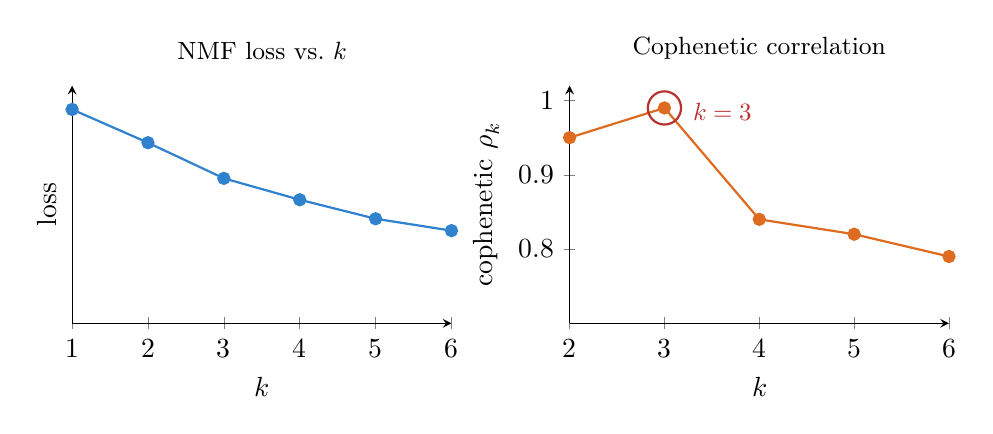
\begin{tikzpicture}
\begin{axis}[name=loss, width=6.4cm, height=4.6cm, axis lines=left, xlabel={$k$}, ylabel={loss}, xtick={1,...,6}, ytick=\empty, title={\small NMF loss vs.\ $k$}, ymin=0, ymax=10]
\addplot[mark=*, thick, dataC] coordinates {(1,9)(2,7.6)(3,6.1)(4,5.2)(5,4.4)(6,3.9)};
\end{axis}
\begin{axis}[at={(loss.east)}, anchor=west, xshift=1.5cm, width=6.4cm, height=4.6cm, axis lines=left, xlabel={$k$}, ylabel={cophenetic $\rho_k$}, xtick={2,...,6}, ymin=0.7, ymax=1.02, ytick={0.8,0.9,1}, title={\small Cophenetic correlation}]
\addplot[mark=*, thick, accentC] coordinates {(2,0.95)(3,0.99)(4,0.84)(5,0.82)(6,0.79)};
\draw[thmred, thick] (axis cs:3,0.99) circle (6pt);
\node[thmred, font=\small, anchor=west] at (axis cs:3.2,0.985) {$k=3$};
\end{axis}
\end{tikzpicture}
\caption{\textbf{Left:} NMF loss keeps falling with $k$. There is often no clean elbow,
and the loss is a different object from a scree plot. \textbf{Right:} cophenetic correlation
measures how \emph{stable} the clustering is across random restarts. Pick $k$ where it peaks
before dropping.}
\end{figure}

\begin{careful}
\textbf{NMF is not nested.} Can I get a rank-$(k-1)$ NMF from a rank-$k$ one? \textbf{No.} You
have to rerun NMF for rank $k-1$. For PCA you can simply drop the last component to get
$k-1$ dimensions, because the PCs are nested. This is also why an NMF loss curve is not
a scree plot: each point on it comes from a separate fit.
\end{careful}

\textbf{Clustering with NMF.} Assign sample $i$ to the part with the largest coefficient,
i.e.\ cluster $j$ if $W^{(r)}_{ij}\ge W^{(r)}_{il}$ for all $l$ (in run $r$).

\begin{definition}{Consensus matrix}{consensus}
Run NMF $T$ times from random initializations. For run $t$ let
\[
C^{(t)}_{ij}=\begin{cases}1&\text{samples } i \text{ and } j \text{ are in the same cluster}\\0&\text{else}\end{cases},
\qquad
C=\frac1T\sum_{t=1}^T C^{(t)}\in[0,1]^{N\times N}.
\]
\end{definition}

\begin{definition}{Cophenetic correlation}{coph}
Treat $1-C$ as a distance between samples and run hierarchical clustering on it (usually
average linkage). The \textbf{cophenetic correlation} $\rho_k$ is the correlation between the
entries of $1-C$ and the tree-induced (cophenetic) distances. If every run agrees, $C$ is
all $0$s and $1$s and $\rho_k=1$. Unstable clusterings give lower $\rho_k$.
\end{definition}

\begin{figure}[htbp]
\centering
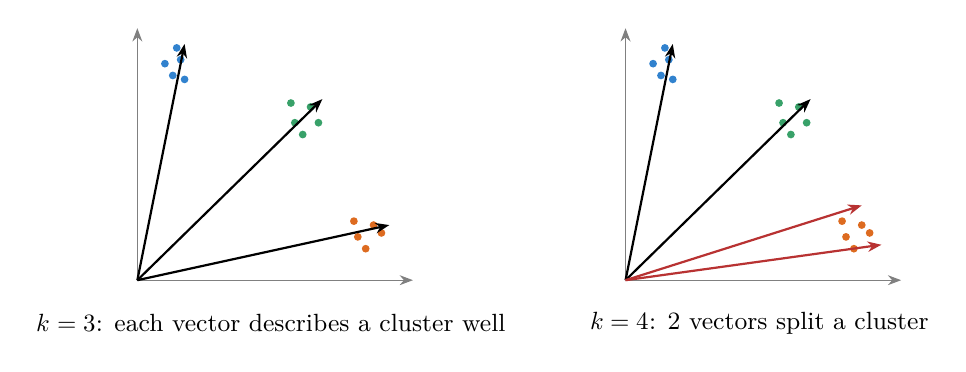
\begin{tikzpicture}[scale=1.0]
\begin{scope}
  \draw[-{Stealth}, gray] (0,0) -- (3.5,0);
  \draw[-{Stealth}, gray] (0,0) -- (0,3.2);
  \foreach \x/\y in {0.45/2.6,0.55/2.8,0.35/2.75,0.6/2.55,0.5/2.95}  \fill[dataC] (\x,\y) circle (1.4pt);
  \foreach \x/\y in {2.0/2.0,2.2/2.2,2.1/1.85,2.3/2.0,1.95/2.25}   \fill[accentD] (\x,\y) circle (1.4pt);
  \foreach \x/\y in {2.8/0.55,3.0/0.7,2.9/0.4,3.1/0.6,2.75/0.75}  \fill[accentC] (\x,\y) circle (1.4pt);
  \draw[-{Stealth[length=5pt]}, thick] (0,0) -- (0.6,3.0);
  \draw[-{Stealth[length=5pt]}, thick] (0,0) -- (2.35,2.3);
  \draw[-{Stealth[length=5pt]}, thick] (0,0) -- (3.2,0.7);
  \node[font=\small, align=center] at (1.7,-0.55) {$k=3$: each vector describes a cluster well};
\end{scope}
\begin{scope}[xshift=6.2cm]
  \draw[-{Stealth}, gray] (0,0) -- (3.5,0);
  \draw[-{Stealth}, gray] (0,0) -- (0,3.2);
  \foreach \x/\y in {0.45/2.6,0.55/2.8,0.35/2.75,0.6/2.55,0.5/2.95}  \fill[dataC] (\x,\y) circle (1.4pt);
  \foreach \x/\y in {2.0/2.0,2.2/2.2,2.1/1.85,2.3/2.0,1.95/2.25}   \fill[accentD] (\x,\y) circle (1.4pt);
  \foreach \x/\y in {2.8/0.55,3.0/0.7,2.9/0.4,3.1/0.6,2.75/0.75}  \fill[accentC] (\x,\y) circle (1.4pt);
  \draw[-{Stealth[length=5pt]}, thick] (0,0) -- (0.6,3.0);
  \draw[-{Stealth[length=5pt]}, thick] (0,0) -- (2.35,2.3);
  \draw[-{Stealth[length=5pt]}, thick, thmred] (0,0) -- (3.25,0.45);
  \draw[-{Stealth[length=5pt]}, thick, thmred] (0,0) -- (3.0,0.95);
  \node[font=\small, align=center] at (1.7,-0.55) {$k=4$: 2 vectors split a cluster};
\end{scope}
\end{tikzpicture}
\caption{Why cophenetic correlation peaks at the true number of clusters. With one
extra component, two vectors compete for the same cluster. Which points go to which
vector then changes from run to run, so the consensus matrix gets fuzzy and $\rho$ drops.}
\end{figure}

\begin{careful}
\textbf{Rows vs.\ columns.} The NMF used for cophenetic correlation (Brunet et al.,
gene-expression data) is set up on the transpose. There, samples are the
\emph{columns} of a genes\,$\times$\,samples matrix and the clustering comes from $H$.
In our row convention (samples = rows), apply NMF to $X\T$ if you want to cluster the
columns. Always check which dimension a method is clustering.
\end{careful}

\subsection{How good can NMF be? A floor from the SVD}

Using the Frobenius loss, define the best achievable NMF error at rank $k$:
\[
\Delta_k=\min_{\substack{W\in\R^{N\times k}_{\ge0}\\ H\in\R^{k\times d}_{\ge0}}}\Fro{X-WH}^2 .
\]

\begin{theorem}{NMF can never beat the truncated SVD}{nmffloor}
If $\sigma_1\ge\sigma_2\ge\cdots$ are the singular values of $X$ (the raw, uncentered $X$), then
\[
\Delta_k\ \ge\ \min_{\rank(B)\le k}\Fro{X-B}^2=\sigma_{k+1}^2+\cdots+\sigma_{\min(N,d)}^2 .
\]
\end{theorem}
\begin{proofsketch}
Every NMF candidate $WH$ is an $N\times d$ matrix of rank at most $k$, because
$\rank(WH)\le\min(\rank W,\rank H)\le k$. So the set of NMF candidates is a
\emph{subset} of the set of all matrices of rank at most $k$. Minimizing the same
function over a smaller set can never give a smaller minimum. The right-hand side is
Eckart--Young (Theorem~\ref{thm:eckart}).
\end{proofsketch}

\begin{intuition}
The truncated SVD $\sum_{i\le k}\sigma_i\vu_i\vv_i\T$ is the unconstrained champion. NMF
competes with its hands tied, since every entry of $W$ and $H$ must be $\ge0$. Its loss
is therefore bounded below by the SVD's. The bound is attained only when some optimal
rank-$k$ approximation happens to factor with nonnegative pieces. In practice the gap
$\Delta_k-\sum_{i>k}\sigma_i^2$ is the \emph{price of interpretability}: the extra error
you accept to get additive, nonnegative parts. Two cautions. The bound is about the
\emph{global} minimum $\Delta_k$, while the algorithms of Section~5.6 may stop at a worse
local minimum. And the comparison uses the \emph{uncentered} SVD of $X$, because NMF
does not center (centered data would have negative entries).
\end{intuition}

\subsection{Interpretability, archetypal analysis and volume penalties}

Because of non-uniqueness, NMF may return parts $\vh_j$ that sit far from every actual data
point (the cone is much wider than the data). Such parts are \textbf{not interpretable} as
``typical examples''. One fix is to add penalties to the reconstruction loss that pull the
parts toward the data.

\begin{definition}{Archetypal analysis}{archetype}
Require each part to be a \emph{convex combination of data points}, $H=BX$, and each
sample to be a convex combination of parts:
\[
\min_{W,B}\ \Fro{X-WBX}^2,\qquad
B=\begin{bmatrix}b_{11}&\cdots&b_{1N}\\\vdots&&\vdots\\b_{k1}&\cdots&b_{kN}\end{bmatrix}\ge0\ \text{with rows summing to }1,
\]
and likewise $W\ge0$ with rows summing to $1$. The rows of $H=BX$ are
\textbf{archetypes}: extreme yet real-looking points on the boundary of the data cloud.
\end{definition}

\textbf{Why ``rows sum to one'' means ``convex hull''.} Row $\ell$ of $X\approx WH$ reads
\[
\vx_\ell\T\approx\sum_{i=1}^{k}W_{\ell i}\,\vh_i\T,\qquad\text{with}\quad \sum_{i=1}^{k}W_{\ell i}=1\ \ \text{for every }\ell .
\]
\begin{itemize}[nosep]
\item Weights that sum to $1$ but may be negative give an \emph{affine} combination. Those
points fill the whole affine hull of $\vh_1,\dots,\vh_k$, the flat through them, which
extends forever. So the sum-to-one constraint \emph{alone does not} put $\vx_\ell$ in the
convex hull (on the board, the arrow to ``convex hull'' was crossed out for this reason).
\item Add $W_{\ell i}\ge0$, which NMF already requires. A nonnegative combination with
weights summing to $1$ is a \emph{convex} combination, so $\vx_\ell$ lies in the
\textbf{convex hull} of the parts: the polygon or polytope with the $\vh_i$ as
corners.
\end{itemize}
The same reasoning applied to $B$ puts every archetype $\vh_i=\sum_jb_{ij}\vx_j$ in the
convex hull of the data. Archetypal analysis therefore asks for a polytope whose corners
sit \emph{inside} the data cloud and which still (approximately) contains it. Its corners
end up at extreme but real points.

\begin{intuition}
\textbf{Convex constraints, non-convex problem.} The word ``convex'' in archetypal analysis
describes the \emph{constraints}: two mixing rules (weighted averages with nonnegative weights that
sum to $1$), used twice:
data $\xrightarrow{\ B\ }$ archetypes $\xrightarrow{\ W\ }$ data. Each constraint set is convex.
The objective $\Fro{X-WBX}^2$ is not jointly convex, because the unknowns multiply each other.
Fix $B$, and the problem in $W$ is a convex least-squares problem; fix $W$, and the same holds for $B$.
So in practice one \textbf{alternates}, exactly like the NMF updates, and lands in a local
optimum. Compared with PCA, which asks ``which \emph{directions} explain the variance?'',
archetypal analysis asks ``which \emph{extreme examples} can every point be mixed from?''.
\end{intuition}

\begin{deeper}
A softer alternative does not \emph{force} the rows of $H$ to be convex combinations
of data. It \textbf{strongly encourages} tightness with a volume penalty
\[
\Fro{X-WH}^2+\gamma\,\operatorname{vol}(H),\qquad \operatorname{vol}(H)=\sqrt{\det(HH\T)} .
\]
$\sqrt{\det(HH\T)}$ is the $k$-dimensional volume of the parallelotope spanned by the
rows of $H$. Shrinking it selects the tightest cone around the data, which removes the
non-uniqueness in the cone figure.
\end{deeper}

\subsubsection*{Why $\sqrt{\det(HH\T)}$ is a volume: the two-vector case}

Take $k=2$ parts, $\vv_1=\vh_1$ and $\vv_2=\vh_2$ (any dimension), with angle $\theta$ between them. They span a
parallelogram. Its area is base $\times$ height, with base $\norm{\vv_1}$.

\begin{figure}[H]
\centering
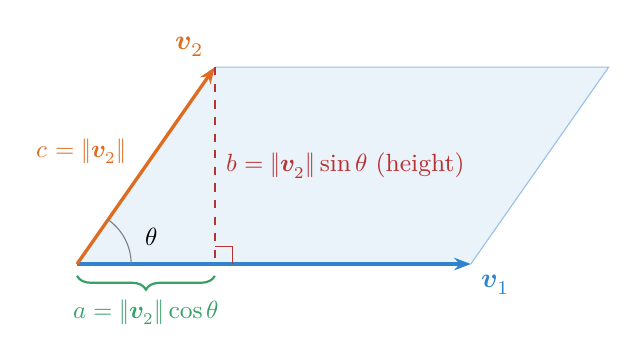
\begin{tikzpicture}[scale=1.25]
  \coordinate (O) at (0,0); \coordinate (V1) at (4,0); \coordinate (V2) at (1.4,2.0);
  \coordinate (F) at (1.4,0);
  \fill[dataC!10] (O)--(V1)--($(V1)+(V2)$)--(V2)--cycle;
  \draw[dataC!50] (V1)--($(V1)+(V2)$)--(V2);
  \draw[-{Stealth[length=6pt]}, very thick, dataC] (O)--(V1) node[below right] {$\vv_1$};
  \draw[-{Stealth[length=6pt]}, very thick, accentC] (O)--(V2) node[above left] {$\vv_2$};
  \draw[dashed, thmred, thick] (V2)--(F);
  \draw[thmred] ($(F)+(0.18,0)$)--($(F)+(0.18,0.18)$)--($(F)+(0,0.18)$);
  \draw[decorate, decoration={brace, amplitude=5pt, mirror}, accentD, thick] (0,-0.12)--(1.4,-0.12)
     node[midway, below=5pt, font=\small] {$a=\norm{\vv_2}\cos\theta$};
  \node[thmred, font=\small, right] at (1.42,1.0) {$b=\norm{\vv_2}\sin\theta$ (height)};
  \node[accentC, font=\small, left] at (0.6,1.15) {$c=\norm{\vv_2}$};
  \draw[gray] (0.55,0) arc (0:55:0.55); \node[font=\small] at (0.75,0.28) {$\theta$};
\end{tikzpicture}
\caption{Split $\vv_2$ into a piece along $\vv_1$ (leg $a$) and a piece perpendicular to $\vv_1$
(leg $b$). With hypotenuse $c=\norm{\vv_2}$ they form a right triangle. Only the height $b$ affects the area.}
\end{figure}

\textbf{The right triangle.} Split $\vv_2$ into the piece along $\vv_1$ and the piece perpendicular to it
(the projection idea from Section~1.1). The three lengths are
\[
c=\norm{\vv_2}\ \ (\text{hypotenuse}),\qquad
a=\norm{\vv_2}\cos\theta\ \ (\text{adjacent leg}),\qquad
b=\norm{\vv_2}\sin\theta\ \ (\text{opposite leg}),
\]
since $\cos=\text{adjacent}/\text{hypotenuse}$ and $\sin=\text{opposite}/\text{hypotenuse}$. Pythagoras, $a^2+b^2=c^2$, reads
\[
(\norm{\vv_2}\cos\theta)^2+(\norm{\vv_2}\sin\theta)^2=\norm{\vv_2}^2(\cos^2\theta+\sin^2\theta)=\norm{\vv_2}^2 .
\]
This is just $\cos^2\theta+\sin^2\theta=1$ scaled by $\norm{\vv_2}^2$. The parentheses matter: the whole leg
is squared, giving $\norm{\vv_2}^2\cos^2\theta$, not $\norm{\vv_2}\cos^2\theta$.

\textbf{From the Gram matrix to the area.} Stack the parts as the rows of $H$, so $HH\T$ is the
$2\times2$ matrix of their dot products, and use $\vv_1\T\vv_2=\norm{\vv_1}\norm{\vv_2}\cos\theta$:
\[
\begin{aligned}
\det(HH\T)&=\det\begin{bmatrix}\norm{\vv_1}^2&\vv_1\T\vv_2\\[2pt]\vv_1\T\vv_2&\norm{\vv_2}^2\end{bmatrix}
=\norm{\vv_1}^2\norm{\vv_2}^2-(\vv_1\T\vv_2)^2\\
&=\norm{\vv_1}^2\norm{\vv_2}^2\,(1-\cos^2\theta)=\big(\norm{\vv_1}\,\norm{\vv_2}\sin\theta\big)^2 .
\end{aligned}
\]
So $\sqrt{\det(HH\T)}=\norm{\vv_1}\cdot\norm{\vv_2}\sin\theta=\text{base}\times\text{height}$. The step $1-\cos^2\theta=\sin^2\theta$ is
exactly the Pythagoras line above.

\begin{intuition}
Only leg $b$ matters for area. Leg $a$ says how far $\vv_2$ reaches \emph{along} $\vv_1$, and sliding the
top edge of a parallelogram sideways (a shear) leaves its area unchanged. So the volume is small
when the parts point in nearly the \emph{same} direction ($\theta\approx0$, height $\approx0$) or are short.
For $k$ parts the same idea repeats: $\sqrt{\det(HH\T)}$ is the product of the successive perpendicular
heights, i.e.\ the lengths of the Gram--Schmidt residuals. In NMF this means the penalty
$\gamma\sqrt{\det(HH\T)}$ rewards parts that are close together and short. They then pinch the cone in
tightly around the data instead of spreading wide (Figure~5).
\end{intuition}

\subsubsection*{Minimum-volume NMF: what the penalty does as it grows}

\textbf{The model.} Add the constraint $W\one=\one$ (each row of $W$ sums to $1$) to NMF, and penalize volume:
\[
\min_{W\ge0,\ H\ge0,\ W\one=\one}\ \Fro{X-WH}^2+\gamma\sqrt{\det(HH\T)} .
\]
The constraint makes each sample a \emph{weighted average} of the parts,
$\vx_i\approx w_{i1}\vh_1+\cdots+w_{ik}\vh_k$ with $w_{ij}\ge0$ and $\sum_jw_{ij}=1$, so the data sit inside the convex hull of
$\vh_1,\dots,\vh_k$ (the argument above). The rows of $H$ are the corners of a simplex, a triangle for $k=3$ and a
tetrahedron for $k=4$, that encloses the data.

\begin{proposition}{Gram determinant and simplex volume}{simplexvol}
For $\vh_1,\dots,\vh_k\in\R^d$ (rows of $H$),
\[
\sqrt{\det(HH\T)}=\underbrace{\operatorname{vol}_k\big(\text{parallelotope on }\vh_1,\dots,\vh_k\big)}_{\text{base}\times\text{heights}}
=k!\cdot\operatorname{vol}_k\big(\operatorname{conv}\{\bm0,\vh_1,\dots,\vh_k\}\big).
\]
\end{proposition}
\begin{proofsketch}
The first equality is the product of perpendicular heights (above). For the second, a simplex fills
$1/k!$ of the parallelotope with the same edges from $\bm0$. In 2D, a triangle is half a parallelogram;
in 3D, a tetrahedron is one sixth of a parallelepiped.
\end{proofsketch}

\begin{careful}
\textbf{Which simplex does the penalty measure?} The data sit in $\operatorname{conv}\{\vh_1,\dots,\vh_k\}$, a
$(k-1)$-dimensional simplex. The penalty measures $\operatorname{conv}\{\bm0,\vh_1,\dots,\vh_k\}$, which also has the
\emph{origin} as a corner. That is a cone over the data simplex, so (cone volume $=\tfrac1k\times$ base $\times$ height)
\[
\sqrt{\det(HH\T)}=(k-1)!\cdot\underbrace{\operatorname{vol}_{k-1}\big(\operatorname{conv}\{\vh_1,\dots,\vh_k\}\big)}_{\text{size of the data simplex}}\cdot\underbrace{\operatorname{dist}\big(\bm0,\operatorname{aff}\{\vh_1,\dots,\vh_k\}\big)}_{\text{its distance from the origin}}.
\]
So the penalty shrinks the enclosing simplex \emph{and} favours placing it close to the origin. The two
goals point the same way (``tight, small parts''), but the penalty is not literally the volume of the
shape that holds the data.
\end{careful}

\begin{figure}[htbp]
\centering
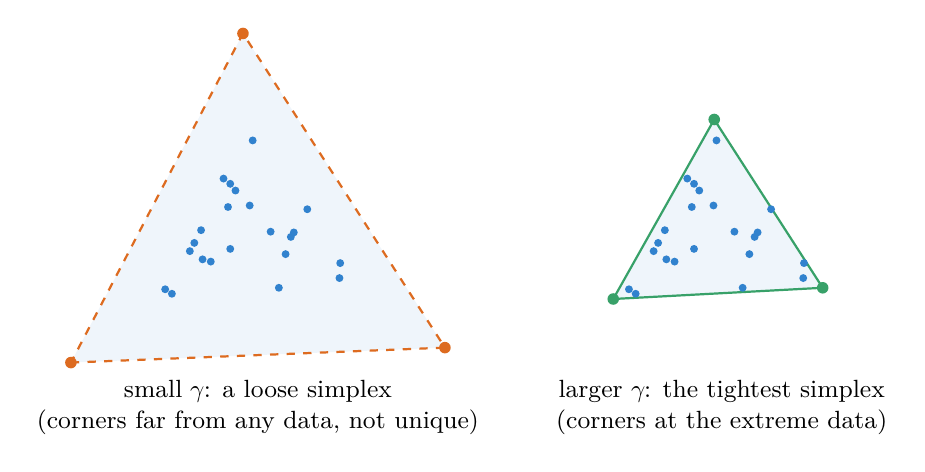
\begin{tikzpicture}[scale=0.95]
\begin{scope}
  \fill[dataC!8] (-0.6,-0.5)--(4.4,-0.3)--(1.7,3.9)--cycle;
  \draw[dashed, accentC, thick] (-0.6,-0.5)--(4.4,-0.3)--(1.7,3.9)--cycle;
  \foreach \p in {(-0.6,-0.5),(4.4,-0.3),(1.7,3.9)} \fill[accentC] \p circle (2.2pt);
  \foreach \x/\y in {0.66/0.48,2.99/0.63,1.83/2.47,2.27/0.95,2.18/0.50,1.05/1.10,3.00/0.83,1.79/1.60,2.56/1.55,2.34/1.18,1.16/0.88,1.50/1.58,1.53/1.02,0.99/0.99,2.07/1.25,1.44/1.96,2.38/1.24,1.60/1.80,1.53/1.89,1.27/0.85,1.14/1.27,0.75/0.42}
    \fill[dataC] (\x,\y) circle (1.5pt);
  \node[font=\small, align=center] at (1.9,-1.1) {small $\gamma$: a loose simplex\\(corners far from any data, not unique)};
\end{scope}
\begin{scope}[xshift=6.2cm]
  \fill[dataC!8] (0.45,0.35)--(3.25,0.5)--(1.8,2.75)--cycle;
  \draw[thick, accentD] (0.45,0.35)--(3.25,0.5)--(1.8,2.75)--cycle;
  \foreach \p in {(0.45,0.35),(3.25,0.5),(1.8,2.75)} \fill[accentD] \p circle (2.2pt);
  \foreach \x/\y in {0.66/0.48,2.99/0.63,1.83/2.47,2.27/0.95,2.18/0.50,1.05/1.10,3.00/0.83,1.79/1.60,2.56/1.55,2.34/1.18,1.16/0.88,1.50/1.58,1.53/1.02,0.99/0.99,2.07/1.25,1.44/1.96,2.38/1.24,1.60/1.80,1.53/1.89,1.27/0.85,1.14/1.27,0.75/0.42}
    \fill[dataC] (\x,\y) circle (1.5pt);
  \node[font=\small, align=center] at (1.9,-1.1) {larger $\gamma$: the tightest simplex\\(corners at the extreme data)};
\end{scope}
\end{tikzpicture}
\caption{Minimum-volume NMF with $W\one=\one$. Both simplices enclose the data and fit it exactly. The volume
penalty picks the tight one, whose corners look like real ``pure'' data points.}
\end{figure}

\textbf{What happens as $\gamma$ increases.}
\begin{itemize}[nosep]
\item $\gamma=0$: any simplex that encloses the data fits equally well. Corners can sit far from the data,
look like no real sample, and change from run to run (the non-uniqueness of Section~5.4).
\item Moderate $\gamma$: volume is expensive, so the corners are pulled inward until the simplex fits
snugly. They stop at the most extreme data points, because shrinking further would leave points outside
and raise the fit error. This is a constrained minimization in effect: shrink the volume, but not past the data.
\item Very large $\gamma$: the penalty dominates. The rows of $H$ are pushed toward each other and become nearly
linearly dependent, the volume collapses toward $0$, and $\Fro{X-WH}$ grows. So $\gamma$ trades fit
against tightness, and it is chosen like any tuning parameter.
\end{itemize}

\begin{intuition}
\textbf{Why this makes NMF interpretable.}
(1) \emph{Parts look like real, pure examples.} The corners sit at the extremes of the data, so each row of
$H$ resembles an actual sample rather than an abstract direction. The classic use is
\textbf{hyperspectral unmixing}: each pixel's spectrum is a mixture of materials, and the corners come out
as the spectra of the pure materials (water, soil, vegetation).
(2) \emph{Each sample reads as a recipe.} Since $\sum_jw_{ij}=1$, row $\bm w_i$ is a set of proportions:
``sample $i$ is $70\%$ part 1, $20\%$ part 2, $10\%$ part 3''.
(3) \emph{The answer is closer to unique.} Many factorizations fit equally well, but the
minimum-volume enclosing simplex is far more constrained. Under conditions on how well the data
fill out the simplex (``sufficiently scattered'' data) it is provably unique up to relabelling. The parts
then reflect structure in the data, not the luck of the initialization.
This is the soft version of archetypal analysis: archetypes are \emph{forced} into the data's hull, while
minimum-volume NMF \emph{pulls} the corners toward it.
\end{intuition}

\subsection{Convex hulls under projection: the shadow picture}

Archetypes, NMF parts and the convex hull all concern the \emph{extreme} points of a data
cloud. A natural shortcut is to run PCA down to 2D and look at the hull there. What does that show?

\begin{proposition}{The shadow of the hull is the hull of the shadows}{hullproj}
Let $P$ be any linear map (for example the projection onto the top $k$ PC directions), and let
$\operatorname{conv}(S)$ be the convex hull of a point set $S$. Then
\[
P\big(\operatorname{conv}(S)\big)=\operatorname{conv}\big(P(S)\big).
\]
The same holds for an affine map $\vx\mapsto P(\vx-\xbar)$, i.e.\ center then project, which is exactly
how PCA scores are computed.
\end{proposition}
\begin{proofsketch}
A point of $\operatorname{conv}(S)$ is a convex combination $\sum_i a_i\vx_i$ ($a_i\ge0$, $\sum a_i=1$). Linearity
gives $P(\sum_ia_i\vx_i)=\sum_ia_iP\vx_i$, a convex combination of the projected points with the
\emph{same} weights. This proves ``$\subseteq$''. Reading the same equation backwards proves ``$\supseteq$''.
For the affine version, $\sum_ia_i(\vx_i-\xbar)=(\sum_ia_i\vx_i)-\xbar$ because the weights sum to $1$.
\end{proofsketch}

\begin{figure}[htbp]
\centering
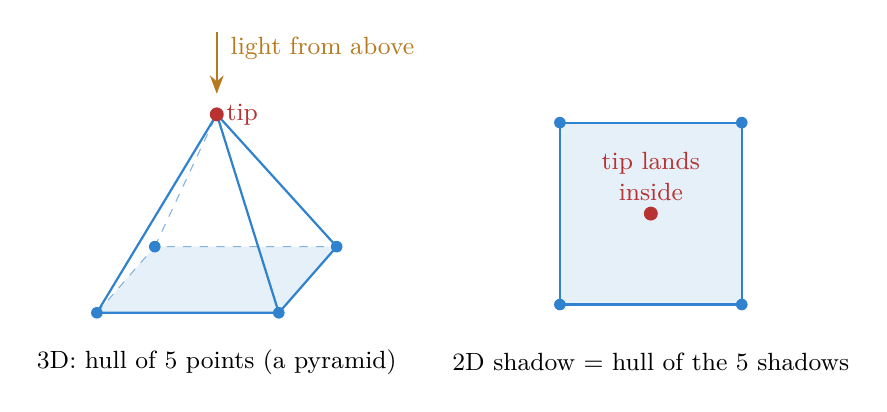
\begin{tikzpicture}[scale=1.05]
\begin{scope}
  % pyramid
  \coordinate (A) at (0,0); \coordinate (B) at (2.2,0); \coordinate (C) at (2.9,0.8); \coordinate (D) at (0.7,0.8);
  \coordinate (T) at (1.45,2.4);
  \fill[dataC!12] (A)--(B)--(C)--(D)--cycle;
  \draw[dataC!60, dashed] (A)--(D)--(C);
  \draw[dataC!60, dashed] (D)--(T);
  \draw[thick, dataC] (A)--(B)--(C);
  \draw[thick, dataC] (A)--(T)--(B); \draw[thick, dataC] (C)--(T);
  \foreach \p in {A,B,C,D} \fill[dataC] (\p) circle (2pt);
  \fill[thmred] (T) circle (2.4pt);
  \node[thmred, font=\small, right] at (T) {tip};
  \draw[-{Stealth}, warnamber, thick] (1.45,3.4) -- (1.45,2.65);
  \node[warnamber, font=\small, right] at (1.5,3.2) {light from above};
  \node[font=\small] at (1.45,-0.6) {3D: hull of 5 points (a pyramid)};
\end{scope}
\begin{scope}[xshift=5.6cm, yshift=0.1cm]
  \fill[dataC!12] (0,0) rectangle (2.2,2.2);
  \draw[thick, dataC] (0,0) rectangle (2.2,2.2);
  \foreach \p in {(0,0),(2.2,0),(2.2,2.2),(0,2.2)} \fill[dataC] \p circle (2pt);
  \fill[thmred] (1.1,1.1) circle (2.4pt);
  \node[thmred, font=\small, align=center] at (1.1,1.55) {tip lands\\inside};
  \node[font=\small, align=center] at (1.1,-0.7) {2D shadow = hull of the 5 shadows};
\end{scope}
\end{tikzpicture}
\caption{The shadow picture. Projecting the pyramid and then taking the hull, or projecting the five
corners and then wrapping a rubber band around them, gives the same square. But the tip, a corner
in 3D, lands in the \emph{interior} of the shadow and looks like an ordinary point.}
\end{figure}

\begin{intuition}
\textbf{The shadow analogy.} Picture a 3D pyramid, the convex hull of its five corners. Shine a
light on it so it casts a shadow on the wall: a projection from 3D to 2D. You can do the two steps in
either order: build the 3D hull and take its shadow, or take each corner's shadow and wrap a
rubber band around those 2D dots. Both give the same shape. PCA is a clever choice of
\emph{where to put the wall}, namely the angle that shows the most spread. So PCA followed by a 2D
hull gives the true shadow of the high-dimensional hull.
\end{intuition}

\begin{careful}
\textbf{A shadow loses information about which points are extreme.} The pyramid's tip is a corner in
3D. Light it from directly above and the tip lands in the middle of the square shadow, where it looks
like an interior point. So the 2D hull does \emph{not} tell you which points are the real extreme
points. The implication runs in only one direction:
\begin{itemize}[nosep]
\item every corner of the shadow comes from a genuine corner of the original hull (the shadow of
an interior point can never stick out past the shadows of the corners), but
\item a genuine corner can vanish into the interior of the shadow.
\end{itemize}
So a PCA plot can confirm that a point is extreme but cannot rule it out. To find
archetypes, work in the full space, or check several projections.
\end{careful}

% ==================================================================
\section{Multidimensional Scaling (MDS)}
% ==================================================================

\subsection{The problem}

We have a set of $N$ objects but no coordinates, only pairwise measurements of
distance or dissimilarity:
\[
D\in\R^{N\times N},\qquad D_{ij}=\text{distance/dissimilarity between objects } i,j,\qquad D_{ii}=0,\quad D_{ij}=D_{ji}.
\]
\textbf{Goal:} find a configuration of points $\vx_1,\dots,\vx_N\in\R^d$ such that
$d(\vx_i,\vx_j)\approx D_{ij}$, so we can plot the objects in a low-dimensional space.

\begin{definition}{Distance matrix}{distmat}
An $N\times N$ matrix $D$ is a \textbf{distance matrix} if
\begin{enumerate}[nosep,label=\arabic*)]
\item it is symmetric, $D=D\T$;
\item $D_{rr}=0$;
\item $D_{rs}\ge0$;
\item $D_{rt}\le D_{rs}+D_{st}$ (triangle inequality).
\end{enumerate}
It is a \textbf{Euclidean distance matrix} if in addition there exist points with
$\norm{\vx_r-\vx_s}_2=D_{rs}$ for all $1\le r,s\le N$.
\end{definition}

\begin{intuition}
\textbf{Distance matrix vs.\ EDM.} A distance matrix just records pairwise distances between
\emph{objects}, which need not be points anywhere: road distances between cities, edit distances
between words. An EDM makes the stronger promise that some configuration of points in ordinary
Euclidean space reproduces those numbers exactly. Every EDM is a distance matrix, but not
conversely. The extra structure is algebraic. With Gram matrix $G=XX\T$,
\[
D_{rs}^2=\norm{\vx_r}^2+\norm{\vx_s}^2-2\vx_r\T\vx_s
\quad\Longleftrightarrow\quad
D\had D=\operatorname{diag}(G)\one\T+\one\operatorname{diag}(G)\T-2G,
\]
where $\operatorname{diag}(G)$ is the vector of diagonal entries. Classical scaling inverts this chain:
\[
\text{distances}\ \longrightarrow\ \text{squared distances}\ \longrightarrow\ \text{centered Gram } B=HAH\ \longrightarrow\ \text{rank}\ \longrightarrow\ \text{dimension}.
\]
\end{intuition}

\subsection{Classical scaling}

Assume $D$ is a Euclidean distance matrix. How do we recover $\vx_1,\dots,\vx_N$?
\textbf{The answer is not unique.} Distances do not change under translation, rotation
or reflection. We remove the translation freedom by assuming the configuration is
centered, $\sum_r\vx_r=\bm0$.

\textbf{Step 1: the Gram matrix.} Let
$B=XX\T=\begin{bmatrix}\vx_1\T\\\vdots\\\vx_N\T\end{bmatrix}[\vx_1\cdots\vx_N]$, so $B_{rs}=\vx_r\T\vx_s$.
\begin{itemize}[nosep]
\item $B$ is \textbf{PSD}: $\bm v\T B\bm v=\bm v\T XX\T\bm v=(X\T\bm v)\T(X\T\bm v)=\norm{X\T\bm v}_2^2\ge0$.
\item $\rank(B)=\rank(X)$.
\end{itemize}

\textbf{Step 2: express $B$ through $D$.}
\[
D_{rs}^2=\norm{\vx_r-\vx_s}^2=\underbrace{\vx_r\T\vx_r}_{B_{rr}}+\underbrace{\vx_s\T\vx_s}_{B_{ss}}-2\underbrace{\vx_r\T\vx_s}_{B_{rs}}
\quad\Longrightarrow\quad
B_{rs}=-\tfrac12\big[D_{rs}^2-B_{rr}-B_{ss}\big].
\]
We still need $B_{rr}$ and $B_{ss}$. Average over one index and use $\sum_s\vx_s=\bm0$:
\begin{align*}
\tfrac1N\textstyle\sum_{s}D_{rs}^2&=\tfrac1N\textstyle\sum_s\big[B_{rr}+B_{ss}-2\vx_r\T\vx_s\big]=B_{rr}+\tfrac1N\tr(B),\\
\tfrac1N\textstyle\sum_{r}D_{rs}^2&=B_{ss}+\tfrac1N\tr(B),\\
\tfrac1{N^2}\textstyle\sum_{r}\sum_sD_{rs}^2&=\tfrac2N\tr(B).
\end{align*}
Solving for $B_{rr}+B_{ss}$ and substituting gives the \textbf{double-centering formula}
\[
B_{rs}=-\tfrac12\Big[D_{rs}^2-\tfrac1N\textstyle\sum_{s'}D_{rs'}^2-\tfrac1N\sum_{r'}D_{r's}^2+\tfrac1{N^2}\sum_{r'}\sum_{s'}D_{r's'}^2\Big].
\]

\begin{proposition}{Matrix form}{doublecenter}
Let $A\in\R^{N\times N}$ with $A_{rs}=-\tfrac12D_{rs}^2$, i.e.\ $A=-\tfrac12\,D\had D$. Then
\[
B=HAH,
\]
where $H$ is the centering matrix. Subtracting row means, then column means, and adding back
the grand mean is exactly what $H(\cdot)H$ does.
\end{proposition}

\begin{algorithm}{Classical scaling}{classical}
Given a distance matrix $D$:
\begin{enumerate}[nosep,label=\arabic*)]
\item compute $A=-\tfrac12\,D\had D$;
\item compute $B=HAH$;
\item eigendecompose $B=U\Lambda U\T$ and take $X=U\Lambda^{1/2}$ (keep the top $t$ eigenpairs for a $t$-dimensional plot).
\end{enumerate}
\end{algorithm}

Step 3 works because $B$ is PSD of rank $d$ with $\lambda_1,\dots,\lambda_d>0$:
\[
B=[\vv_1\cdots\vv_d\,|\,\vv_{d+1}\cdots\vv_N]
\begin{bmatrix}\Lambda_d&0\\0&0\end{bmatrix}
\begin{bmatrix}\vv_1\T\\\vdots\\\vv_N\T\end{bmatrix}
=[\vv_1\cdots\vv_d]\,\Lambda_d^{1/2}\,\Lambda_d^{1/2}\,[\vv_1\cdots\vv_d]\T
=\underbrace{(V_d\Lambda_d^{1/2})}_{X}\underbrace{(V_d\Lambda_d^{1/2})\T}_{X\T}.
\]
We cannot use $B=XX\T$ directly because we do not know $X$. We only know $D$, and
from it we build $B$. Any $XQ$ with $Q$ orthogonal works equally well, so we are free
to rotate the data after finding the low-dimensional representation.

\begin{theorem}{Characterization of Euclidean distance matrices}{edm}
A distance matrix $D$ is Euclidean \textbf{if and only if} $B=HAH$ is positive semidefinite,
i.e.\ all its eigenvalues are $\ge0$. The embedding dimension is $\rank(B)$.
\end{theorem}

\begin{example}{Equilateral triangle}{tri}
\[
D=\begin{bmatrix}0&1&1\\1&0&1\\1&1&0\end{bmatrix}\ \Rightarrow\
A=-\tfrac12(\one\one\T-I),\quad
B=HAH=\tfrac12H=\begin{bmatrix}\tfrac13&-\tfrac16&-\tfrac16\\-\tfrac16&\tfrac13&-\tfrac16\\-\tfrac16&-\tfrac16&\tfrac13\end{bmatrix},
\]
with eigenvalues $\tfrac12,\tfrac12,0$. $B$ is PSD, so $D$ is Euclidean, and the rank is $2$:
three equidistant points live in a plane, as an equilateral triangle with side $1$.
\end{example}

\begin{example}{A dissimilarity that is not Euclidean}{noneuc}
$D=\begin{bmatrix}0&1&3\\1&0&1\\3&1&0\end{bmatrix}$ is \emph{not Euclidean}. Indeed it violates the
triangle inequality, $D_{13}=3>D_{12}+D_{23}=2$. Classical scaling detects this:
\[
B=HAH=\begin{bmatrix}\tfrac{19}{9}&\tfrac{5}{18}&-\tfrac{43}{18}\\[2pt]\tfrac{5}{18}&-\tfrac59&\tfrac{5}{18}\\[2pt]-\tfrac{43}{18}&\tfrac{5}{18}&\tfrac{19}{9}\end{bmatrix},
\qquad\text{eigenvalues } \tfrac92,\ 0,\ -\tfrac56 .
\]
A PSD matrix must have nonnegative diagonal entries ($B_{rr}=\bm e_r\T B\bm e_r\ge0$), so
$B_{22}=-\tfrac59$ is already an immediate red flag. The negative eigenvalue (eigenvector
$\propto(1,-2,1)$) confirms it.
\end{example}

\begin{example}{City blocks are not Euclidean in any dimension}{manhattan}
Take four street corners $A=(0,0)$, $B=(1,0)$, $C=(0,1)$, $D=(1,1)$ with \textbf{Manhattan} (city-block) distance
$|x_1-y_1|+|x_2-y_2|$:
\[
AB=AC=BD=CD=1,\qquad AD=BC=2 .
\]
Every triangle inequality holds, so this is a genuine distance matrix. Yet no points in \emph{any}
$\R^m$ realize it:
\begin{itemize}[nosep]
\item $AB+BD=1+1=2=AD$. In Euclidean space a route can equal the straight-line distance only if
it \emph{is} the straight line, so $B$ must be the midpoint of $A$ and $D$: $B=\tfrac12(A+D)$.
\item By the same argument with $C$: $AC+CD=2=AD$, so $C=\tfrac12(A+D)$ too.
\item Then $B=C$, but the matrix says $BC=2$. Contradiction.
\end{itemize}
Classical scaling agrees. Ordering the points $A,B,C,D$,
\[
B_{\text{mat}}=HAH=\frac14\begin{bmatrix}3&1&1&-5\\1&3&-5&1\\1&-5&3&1\\-5&1&1&3\end{bmatrix},
\qquad\text{eigenvalues } 2,\ 2,\ 0,\ -1,
\]
with the negative eigenvalue on $(1,-1,-1,1)$.
\end{example}

\begin{intuition}
Extra dimensions give a path more directions to \emph{bend} in, and bending only makes it
longer. They cannot let two different points both be the unique midpoint of the same segment.
The ``straight line is the only shortest path'' rule holds in $\R^2$, $\R^3$ and $\R^{100}$ alike, so no
embedding dimension fixes this. (Manhattan geometry has many shortest paths between two
corners, which is precisely what Euclidean geometry forbids.)
\end{intuition}

\textbf{Seeing it work: a map from nothing but distances.} Give classical scaling only the great-circle distances between ten US cities, with no coordinates at all, and it draws the map (Figure~\ref{fig:mdscities}).

\begin{figure}[htbp]
\centering
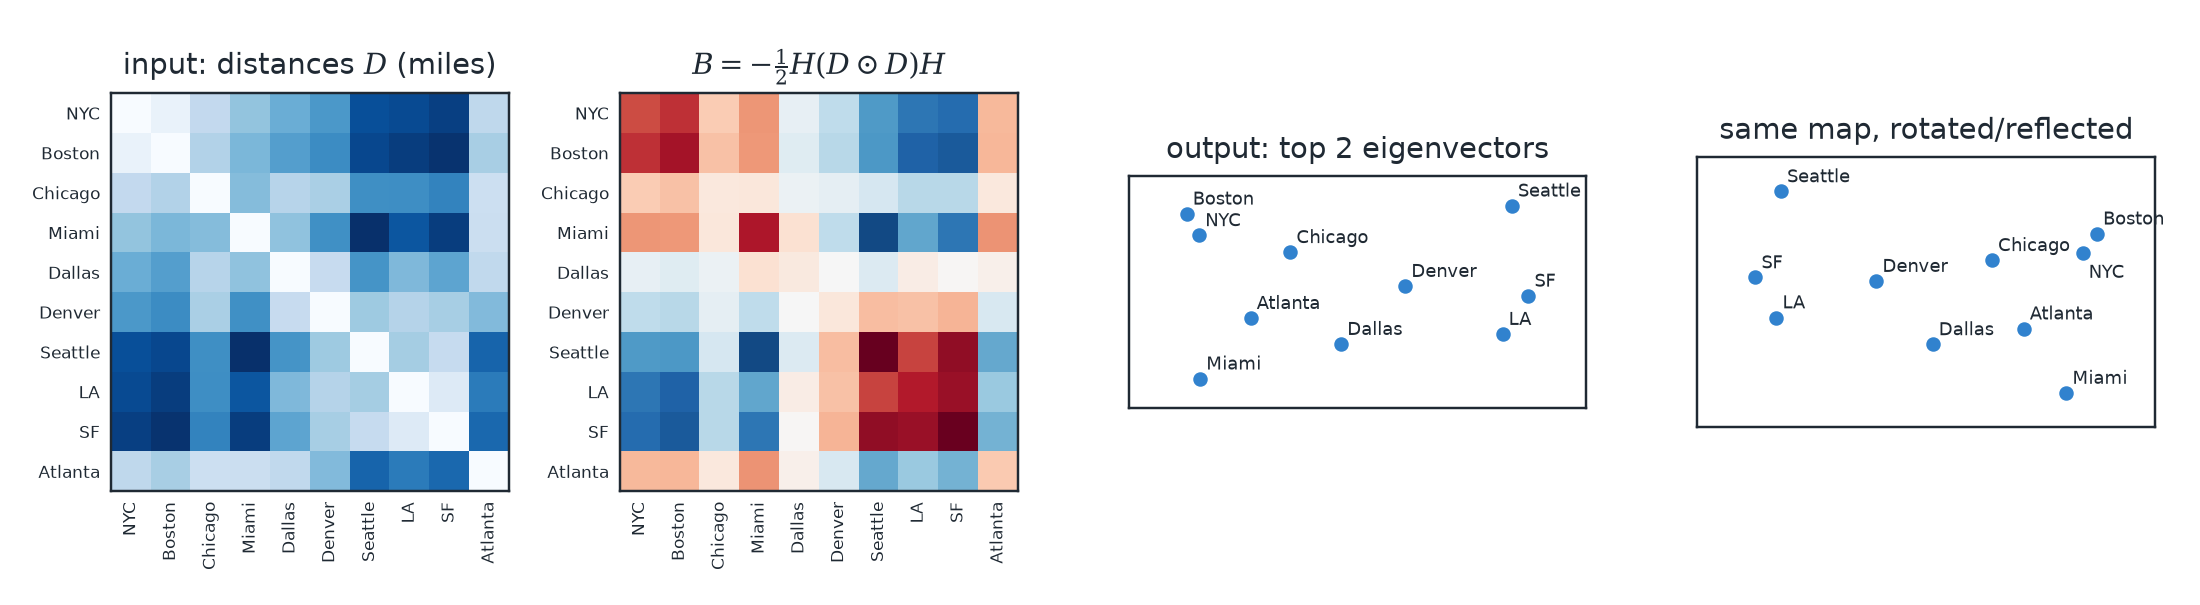
\includegraphics[width=\textwidth]{figures/mds_cities.png}
\caption{Classical scaling on ten cities, using distances computed from their latitudes and longitudes. The double-centered matrix $B$ is positive where two cities lie on the same side of the center and negative where they lie on opposite sides (Seattle and Miami). The raw output is correct but can come out in any orientation, since distances cannot tell north from south; here a rotation and a reflection line it up with a normal map. Median error in distance: $0.13\%$ (NYC--LA is $2445$ miles in, $2446$ out).}
\label{fig:mdscities}
\end{figure}

\subsubsection*{Weighted Euclidean distances are still Euclidean}

A common dissimilarity weights directions differently:
$d_W(\vx,\vy)^2=(\vx-\vy)\T W(\vx-\vy)$ for a symmetric PSD matrix $W$. Is a matrix of such
distances Euclidean, so that classical scaling applies without negative eigenvalues? Yes.

\begin{proposition}{A weighted distance is a sum of squared projections}{weighted}
Write $W=U\Lambda U\T$ (spectral theorem, with $\lambda_i\ge0$ since $W$ is PSD) and $\bm z=\vx-\vy$. Then
\[
d_W(\vx,\vy)^2=\bm z\T U\Lambda U\T\bm z=\sum_{i=1}^d\lambda_i\big(\vu_i\T(\vx-\vy)\big)^2
=\norm{\Lambda^{1/2}U\T\vx-\Lambda^{1/2}U\T\vy}_2^2 .
\]
\end{proposition}
\begin{proofsketch}
$U\T\bm z=(\vu_1\T\bm z,\dots,\vu_d\T\bm z)\T$ is the list of projections of $\bm z$
onto the orthonormal eigenvectors. So $\bm z\T U\Lambda U\T\bm z=(U\T\bm z)\T\Lambda(U\T\bm z)$
is a weighted sum of squared projections. For the last equality, set $A=\Lambda^{1/2}U\T$.
Then $A\T A=U\Lambda U\T=W$, so $\bm z\T W\bm z=\bm z\T A\T A\bm z=\norm{A\bm z}^2$.
\end{proofsketch}

\begin{intuition}
Read $A=\Lambda^{1/2}U\T$ right to left: \emph{rotate} into the eigenvector axes, then
\emph{stretch} axis $i$ by $\sqrt{\lambda_i}$. A weighted distance is the ordinary
distance after this linear map, so the points $A\vx_1,\dots,A\vx_N$ realize it exactly.
That means the distance matrix is Euclidean and $B=HAH$ is PSD. Classical scaling
returns the configuration $A\vx_i$, up to rotation. Example: with $W=\diag(4,1)$,
$d_W^2=4(x_1-y_1)^2+(x_2-y_2)^2$. A step in the $x_1$ direction counts double
($\sqrt4=2$).
\end{intuition}

\begin{deeper}
Two familiar special cases. \textbf{Standardizing} the variables before PCA is the choice
$W=\diag(1/s_1^2,\dots,1/s_d^2)$ (Section~2.5). The \textbf{Mahalanobis distance}
$d_M^2=(\vx-\vy)\T\Sig^{-1}(\vx-\vy)=\sum_i(\vw_i\T(\vx-\vy))^2/\lambda_i$ uses the
PCA axes and \emph{divides} by the PC variances. Low-variance directions count more, and
the map $A=\Lambda^{-1/2}[\vw_1\cdots\vw_d]\T$ (PCA loadings, not the weight matrix) is exactly \textbf{whitening}: after it, the data have
identity covariance.
\end{deeper}

\subsection{Handling negative eigenvalues}

Real dissimilarities are often not Euclidean, so $B$ has some negative eigenvalues:
\[
B=[\vv_1\cdots\vv_N]\diag(\lambda_1,\dots,\lambda_N)[\vv_1\cdots\vv_N]\T,\qquad
\lambda_1\ge\cdots\ge\lambda_{t_0}>0>\lambda_{t_0+1}\ge\cdots\ge\lambda_N .
\]
\begin{itemize}
\item \textbf{Option 1 (ignore them):} keep only the top $t\le t_0$ positive eigenpairs,
\[X_t=[\vv_1\cdots\vv_t]\,\diag(\lambda_1,\dots,\lambda_t)^{1/2}.\]
This is the standard choice.
\item \textbf{Option 2 (additive constant):} add a constant $c$ to all off-diagonal $D_{rs}$ until the
distances are all Euclidean. This works in principle but distorts every distance, so it is rarely preferred.
\end{itemize}

\textbf{Seeing negative eigenvalues.} Negative eigenvalues are a fingerprint of distances that no flat picture can reproduce. Compare two ways of measuring distance between the same $40$ points on a circle (Figure~\ref{fig:mdsneg}). The cities above show a mild case: the Earth's curvature gives eigenvalues of $B$ as low as $-4\times10^{4}$, which is tiny next to the top two ($9.9\times10^{6}$ and $1.8\times10^{6}$).

\begin{figure}[htbp]
\centering
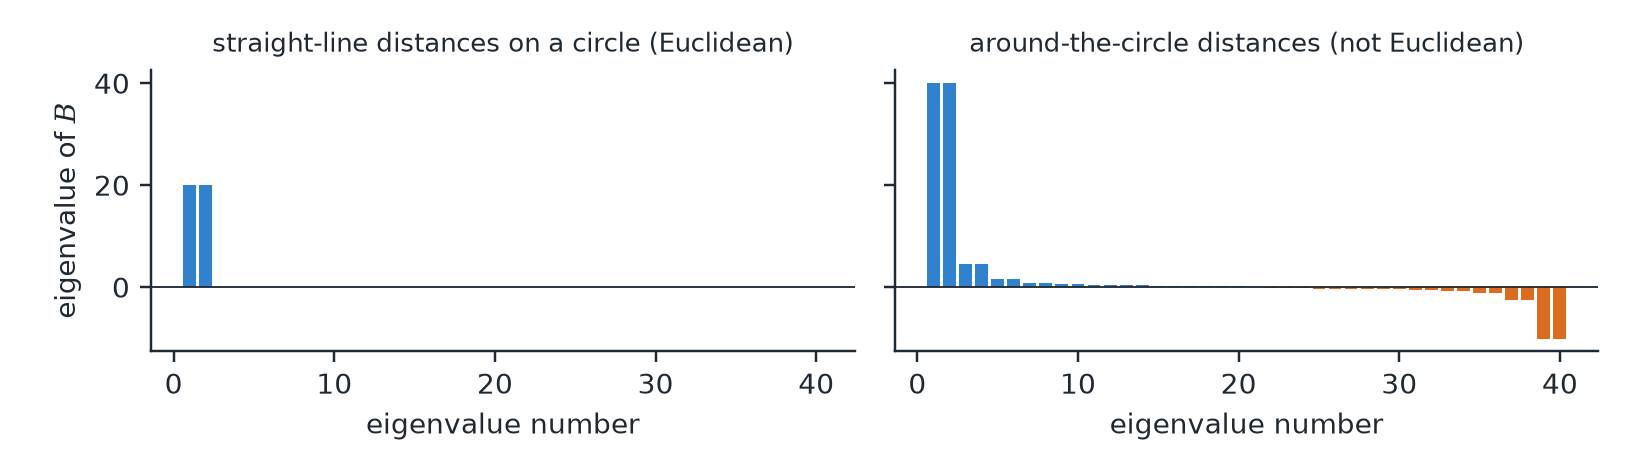
\includegraphics[width=\textwidth]{figures/mds_negative.png}
\caption{\emph{Left:} straight-line distances are Euclidean, so $B$ is PSD with exactly two non-zero eigenvalues ($20,20$), the circle's true dimension in $\R^2$. \emph{Right:} distances measured around the circle cannot all be matched by points in any Euclidean space, and $B$ gets negative eigenvalues (down to $-10.08$). This is the matrix Isomap would use on a closed loop.}
\label{fig:mdsneg}
\end{figure}

\subsection{Duality of classical scaling and PCA}

Start with data $\vx_1,\dots,\vx_N\in\R^d$, construct the distance matrix using Euclidean
distance, and then apply classical scaling:
\[
X\ \longrightarrow\ D\ \longrightarrow\ A\ \longrightarrow\ B=HAH .
\]
By the centering assumption (distances do not see the mean),
\[
B=HAH=(HX)(HX)\T .
\]
If $HX=USV\T$, then
\[
B=(USV\T)(USV\T)\T=US\,S\T U\T=US^2U\T .
\]
The eigenvalues of $B$ are $\sigma_j^2$ (that is, $N\lambda_j$), and the classical-scaling
embedding is $US$. This is \textbf{exactly the PC score matrix}.

\begin{theorem}{Classical scaling = PCA}{dual}
Classical scaling on Euclidean distances between $\vx_1,\dots,\vx_N$ returns the PCA scores,
up to an orthogonal transformation (sign flips and rotations within tied eigenvalues).
\end{theorem}

\subsubsection*{PCA three ways}\label{sec:threeways}
\begin{enumerate}[nosep,label=\arabic*)]
\item compute the sample covariance $\Sig=\tfrac1N X\T HX$ ($d\times d$) and diagonalize it;
\item center the data and take the SVD $HX=USV\T$;
\item eigendecompose the centered Gram matrix $HXX\T H$ ($N\times N$); then $US$ gives the scores.
\end{enumerate}
\textbf{If $N\ll d$} (e.g.\ 100 patients $\times$ 20{,}000 genes), route 3 diagonalizes an
$N\times N$ matrix instead of a $d\times d$ one, which is much cheaper. It is also the route
that generalizes to kernels.

\begin{careful}
When you plot the eigenvalues of $B$ to choose a dimension, remember that scale issues
carry over from PCA. Check the units of the original variables and make sure there are no
issues with scale before you trust the rank you read off.
\end{careful}

\subsection{How good is a $t$-dimensional embedding? (strain)}

With $X=USV\T$,
\[
B=XX\T=US\,S\T U\T=\sum_{i}\sigma_i^2\,\vu_i\vu_i\T \qquad (S\T=S \text{ in the square case, since it is diagonal}).
\]
The best $t$-dimensional configuration is $Y^\star=U_tS_t$ ($N\times t$ times $t\times t$). Then
\[
XX\T-Y^\star Y^{\star\mathsf T}=\sum_{i=t+1}^{d}\sigma_i^2\,\vu_i\vu_i\T .
\]
Each $\vu_i\vu_i\T$ sets a direction, and $\sigma_i^2$ determines its magnitude. Because the
$\vu_i\vu_i\T$ are orthonormal in the Frobenius inner product,
\[
\Fro{XX\T-Y^\star Y^{\star\mathsf T}}^2=\sum_{i=t+1}^d\sigma_i^4,
\qquad
\Fro{XX\T}^2=\sum_{i=1}^d\sigma_i^4,
\]
where $\Fro{A}^2=\sum_{i,j}A_{ij}^2$ is the sum of all entries squared. Entrywise, the error
is $(XX\T-YY\T)_{ij}=\vx_i\T\vx_j-\vy_i\T\vy_j$, a mismatch of inner products.

\begin{definition}{Relative strain}{strain}
\[
F_t=\left(\frac{\sum_{i=t+1}^d\sigma_i^4}{\sum_{i=1}^d\sigma_i^4}\right)^{1/2}\in[0,1].
\]
Small $F_t$ means the $t$-dimensional picture preserves the inner products well.
\end{definition}

\begin{deeper}
Compare this with PCA's PVE. PCA measures squared reconstruction error of the
\emph{points}, $\sum_{i>t}\sigma_i^2$. Strain measures error in the \emph{Gram matrix},
$\sum_{i>t}\sigma_i^4$. Squaring again weights the large singular values even more heavily.
\end{deeper}

\subsection{Metric MDS}

Classical scaling treats the dissimilarities as Euclidean distances. \textbf{Metric MDS}
is more flexible. Given a distance matrix $D$, we want to find $\vy_1,\dots,\vy_N\in\R^t$ such that
\[
d(\vy_i,\vy_j)\approx f(D_{ij}),
\]
where $f$ is a \textbf{monotonically increasing} function of $D_{ij}$ and $d$ can be non-Euclidean.
The usual choice is $f(D_{ij})=\alpha+\beta D_{ij}$ with $\alpha\ge0$, $\beta>0$:
\begin{itemize}[nosep]
\item \textbf{absolute MDS:} $\alpha=0,\ \beta=1$ (match the distances exactly);
\item \textbf{ratio MDS:} $\alpha=0,\ \beta>0$ (match up to an overall scale);
\item \textbf{interval MDS:} $\alpha\ge0,\ \beta>0$ (match up to scale and shift).
\end{itemize}

\begin{deeper}
There is no eigendecomposition shortcut here. One minimizes a \emph{stress} criterion such
as $\sum_{i<j}\big(d(\vy_i,\vy_j)-f(D_{ij})\big)^2$ numerically, e.g.\ with the SMACOF
majorization algorithm. Classical scaling's output is a common initialization.
\end{deeper}

% ==================================================================
\section{Kernel PCA}\label{sec:kpca}
% ==================================================================

\subsection{Motivation: data on curved surfaces}

\begin{figure}[htbp]
\centering
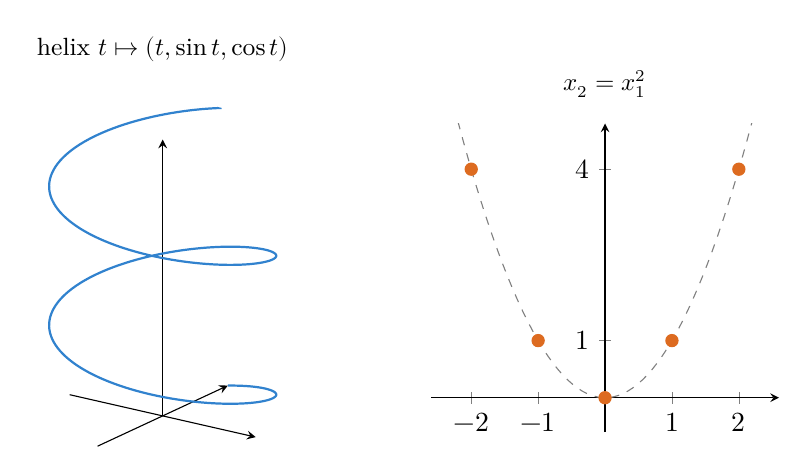
\begin{tikzpicture}
\begin{axis}[name=helix, view={35}{15}, width=5.6cm, height=6.4cm, axis lines=center, ticks=none,
  xlabel={}, ylabel={}, zlabel={}, title={\small helix $t\mapsto(t,\sin t,\cos t)$}]
\addplot3[domain=0:12.5, samples=240, samples y=0, thick, dataC] ({sin(deg(x))},{cos(deg(x))},{x});
\end{axis}
\begin{axis}[at={(helix.east)}, anchor=west, xshift=1.4cm, width=6cm, height=5.5cm, axis lines=middle, xmin=-2.6, xmax=2.6, ymin=-0.6, ymax=4.8,
  xtick={-2,-1,1,2}, ytick={1,4}, title={\small $x_2=x_1^2$}]
\addplot[domain=-2.2:2.2, samples=60, gray, dashed] {x^2};
\addplot[only marks, mark=*, accentC, mark size=2.2pt] coordinates {(-2,4)(-1,1)(0,0)(1,1)(2,4)};
\end{axis}
\end{tikzpicture}
\caption{\textbf{Left:} a helix, drawn with the $t$-axis vertical, is a 1-dimensional curve in $\R^3$. PCA
needs all 3 dimensions to contain it, because no line or plane does. NMF does nothing useful here, since the
coordinates take negative values. \textbf{Right:} the five points $X=\{(-2,4),(-1,1),(0,0),(1,1),(2,4)\}$
live in $\R^2$ on the parabola $x_2=x_1^2$. One coordinate should be enough to reconstruct them.}
\end{figure}

\begin{definition}{Ambient, intrinsic and linear dimension}{dims}
For a data set in $\R^d$:
\begin{itemize}[nosep]
\item the \textbf{ambient dimension} is $d$, the number of coordinates we record;
\item the \textbf{intrinsic dimension} is the number of free parameters that generate the points
(for the helix, $1$: knowing $t$ fixes the point);
\item the \textbf{linear (PCA) dimension} is the dimension of the smallest affine subspace containing
the points, i.e.\ the number of nonzero PC variances.
\end{itemize}
Always: intrinsic $\le$ linear $\le$ ambient. For the helix: $1\le 3\le 3$.
\end{definition}

\begin{intuition}
\textbf{What PCA and NMF do to a helix.} A $1$-PC PCA model is $\vx\approx\xbar+z\,\vw_1$.
Every reconstruction lies on one straight line. If the helix is stretched out
(many turns along $t$), $\vw_1$ points roughly along the axis, and the score $z$ increases
with $t$. That is a useful summary of ``how far along'' a point is, but the reconstruction
collapses each turn of the coil onto the line. Two PCs give a plane, which is better but
still flat. Only three PCs reproduce the helix exactly. NMF is also a linear model (a cone
instead of a subspace). It needs the data shifted to be nonnegative first, and it still
cannot bend. Neither method can \emph{unroll} the curve. They rotate and project.
\end{intuition}

\textbf{The idea of kernel PCA:} ``linear'' depends on which features you hand the method.
Map the data through nonlinear features so that the curved structure becomes \emph{flat} in
feature space, then run ordinary PCA there. For the helix, the features
$(\cos t,\sin t)\mapsto\operatorname{atan2}(\sin t,\cos t)$ would recover the angle. For the
parabola, one extra feature is enough:

\begin{example}{Making a parabola linear}{parab}
Use the features
\[\varphi(x_1,x_2)=(x_1,\ x_2,\ x_1^2).\]
The five points map to $(-2,4,4)$, $(-1,1,1)$, $(0,0,0)$, $(1,1,1)$, $(2,4,4)$. The second and third features are
\emph{identical}, so the feature covariance has a zero eigenvalue with eigenvector
$\propto(0,1,-1)$. By the implicit description of zero-variance directions
(Section~3.3), the data satisfy $\big(0,1,-1\big)\cdot(\varphi(\vx)-\bar{\varphi})=0$, i.e.\
$x_2-x_1^2=0$. \textbf{Zero eigenvalues in feature space give the implicit equation of the nonlinear surface.}
Compare Section~2.6: on the raw coordinates, $\operatorname{cov}(x_1,x_1^2)=0$ for these points, so
ordinary PCA saw no relationship at all.
\end{example}

\begin{example}{What does ordinary PCA find on a circle?}{pcacircle}
Take points spread evenly around the unit circle, $\vx=(\cos\theta,\sin\theta)$ with $\theta$ uniform. The mean is $\bm0$ and,
since $\mathbb E\cos^2\theta=\mathbb E\sin^2\theta=\tfrac12$ and $\mathbb E\cos\theta\sin\theta=0$,
\[
\Sig=\begin{bmatrix}\tfrac12&0\\0&\tfrac12\end{bmatrix}=\tfrac12I,\qquad \lambda_1=\lambda_2=\tfrac12 .
\]
\begin{itemize}[nosep]
\item \textbf{Two nonzero variances.} No line contains the circle, so PCA needs both dimensions (linear dimension $2$),
even though the circle has one degree of freedom, the angle (intrinsic dimension $1$).
\item \textbf{The loadings are not ``one in $x$, one in $y$'' specifically.} With a tied eigenvalue, \emph{every} unit vector is an
eigenvector of $\tfrac12I$ (variance is the same in every direction, as you said), so \emph{any} orthonormal pair is a valid
answer. Software returns an arbitrary pair, often decided by sampling noise, which makes the two finite-sample
eigenvalues slightly unequal. The axes $x$ and $y$ are one valid choice among infinitely many.
\item Scree plot: flat, $50\%$ of the variance each. PCA correctly reports ``no preferred direction'' but cannot report
``these points lie on a curve''. For that, add features (next).
\end{itemize}
\end{example}

\subsubsection*{How a curved equation becomes a linear one}

Lift the circle with the quadratic features $\varphi(\vx)=(f_1,\dots,f_5)=(x_1,\,x_2,\,x_1^2,\,x_2^2,\,x_1x_2)$. The circle's equation is
\[
x_1^2+x_2^2=1\quad\Longleftrightarrow\quad 0\cdot f_1+0\cdot f_2+1\cdot f_3+1\cdot f_4+0\cdot f_5=1\quad\Longleftrightarrow\quad \vw\T\varphi(\vx)=1,\ \ \vw=(0,0,1,1,0).
\]
``Linear'' means linear in the \emph{features}: the equation is a fixed weighted sum of the $f$'s, with constant coefficients
$\vw$. All of the nonlinearity has been moved \emph{inside} the features ($f_3=x_1^2$ is a nonlinear function of $x_1$), so
\emph{between} features the relationship is a flat one. Geometrically, every lifted point $\varphi(\vx_i)\in\R^5$ lies on the
hyperplane $\{\bm f:\vw\T\bm f=1\}$. After centering, $\vw\T(\varphi(\vx_i)-\bar\varphi)=1-1=0$ for every $i$, so the variance along
$\vw/\norm{\vw}$ is exactly $0$: PCA on the lifted data returns a \textbf{zero PC variance with loading
$\propto(0,0,1,1,0)$}, and reading that loading back gives the equation $x_1^2+x_2^2=\text{const}$. (Same idea as $y=x^2$: a
curve in $(x,y)$, but the flat relation ``coordinate $2=$ coordinate $3$'' in the features $(x,\,y,\,x^2)$.)

\begin{careful}
\textbf{How do you know if you lifted enough, or too much?}
\begin{itemize}[nosep]
\item \textbf{Enough} means the features include every monomial in the true relation. With degree $\le1$ features (just
$x_1,x_2$) the circle shows no zero variance at all. With degree $\le2$ exactly one zero variance appears: the circle. If
you included $x_1^2$ but forgot $x_2^2$, the relation is invisible. So the practical test is to raise the degree step
by step and watch for (near-)zero variances to \emph{appear}.
\item \textbf{Too many} brings three problems. (a) \emph{Consequences of the same relation}: with degree $\le3$ (9 features) the
circle gives \textbf{three} zero variances, from $g=x_1^2+x_2^2-1$, $x_1g$ and $x_2g$, which are all the same circle, not new
structure. (b) \emph{Too few points}: once the number of features reaches $N-1$, zero variances appear automatically
(Prop.~\ref{prop:nminus1}), real structure or not. (c) Cost: $d'$ grows like $d^h$.
\item With noisy data look for \emph{small}, not exactly zero, variances, and check on held-out data (Section~\ref{sec:preimage}).
\end{itemize}
(Checked numerically on points of the unit circle: $0$, $1$ and $3$ zero variances for degrees $1$, $2$, $3$.)
\end{careful}

\subsection{Explicit feature maps and why they blow up}

Let $\varphi:\R^d\to\R^{d'}$ define features, e.g.\ all quadratic monomials
\[
\varphi(x_1,x_2)=(x_1,\ x_2,\ x_1^2,\ x_2^2,\ x_1x_2),\qquad \R^2\to\R^5 .
\]
The pipeline is
\[
\underbrace{X}_{\R^{N\times d}}\ \xrightarrow{\ \varphi\ }\ \underbrace{\widetilde X}_{\R^{N\times d'}}
\ \xrightarrow{\ \text{zero evals}\ }\ \underbrace{M}_{\substack{\text{nonlinear surface}\\\text{(implicit equations)}}}
\ \xrightarrow{\ \text{rotate (PC)}\ }\ \underbrace{Y}_{\substack{\text{scores = coordinates}\\\text{on the surface}}} .
\]
But $d'$ grows very quickly. With all monomials up to degree $h$,
\[
d'=\binom{d+h}{h}-1\ \approx\ d^h .
\]
\begin{center}
\renewcommand{\arraystretch}{1.2}
\begin{tabular}{r|rr}
$d$ & quadratic ($h=2$) & cubic ($h=3$)\\\hline
2 & 5 & 9 \\
10 & 65 & 285 \\
20 & 230 & 1770
\end{tabular}
\end{center}
Here $h$ is the degree of the polynomials you include. Explicit features therefore bring
two problems: \textbf{computation} (huge $d'\times d'$ covariance matrices) and
\textbf{overfitting} (with $d'\gg N$, almost any curve fits).

\subsection{The kernel trick}

\begin{definition}{Kernel PCA setup}{kpcasetup}
Let $\varphi:\R^d\to\mathcal F$ be a feature map into a \textbf{feature space} $\mathcal F$
(think $\R^{D}$ with $D$ huge, possibly $D=\infty$), and write the centered features as
\[
\tilde\varphi_i=\varphi(\vx_i)-\bar{\varphi},\qquad \bar{\varphi}=\tfrac1N\textstyle\sum_{i}\varphi(\vx_i),\qquad
\widetilde\Phi=H\widetilde X=\begin{bmatrix}\tilde\varphi_1\T\\\vdots\\\tilde\varphi_N\T\end{bmatrix}\in\R^{N\times D}.
\]
Kernel PCA is ordinary PCA of $\varphi(\vx_1),\dots,\varphi(\vx_N)$: diagonalize
$\Sig_\varphi=\tfrac1N\widetilde\Phi\T\widetilde\Phi$ ($D\times D$) and report the scores
$\vw_j\T\tilde\varphi_i$.
\end{definition}

What is the \emph{cheapest} way to compute the PC scores? Use two properties.
\begin{enumerate}
\item By PCA route 3, the scores come from the centered Gram matrix:
\[
\widetilde\Phi\,\widetilde\Phi\T=H\big[\varphi(\vx_i)\T\varphi(\vx_j)\big]_{i,j}H=HKH=\widetilde K,
\qquad K_{ij}=\varphi(\vx_i)\T\varphi(\vx_j).
\]
The eigendecomposition of $\widetilde K$ gives the PC scores and variances (proved below). \textbf{Only inner products of features are needed.}
\item For some choices of $\varphi$ there is a function $k:\R^d\times\R^d\to\R$ with
\[
k(\vx,\vy)=\langle\varphi(\vx),\varphi(\vy)\rangle_{\mathcal F}=\varphi(\vx)\T\varphi(\vy)
\]
that is \textbf{cheap} to evaluate (cost $O(d)$, not $O(D)$). This is the \textbf{kernel trick}.
\end{enumerate}

\begin{intuition}
\textbf{Where are the dot products in ordinary PCA?} You usually see PCA as an SVD, $HX=USV\T$. But the
scores are $US$, and $U$ and $S$ are exactly what you get from the eigendecomposition of the \emph{Gram matrix}
\[
(HX)(HX)\T=US^2U\T,\qquad \big[(HX)(HX)\T\big]_{ij}=(\vx_i-\xbar)\T(\vx_j-\xbar)\quad\text{(a dot product)}.
\]
So the scores depend on the data \emph{only through the table of pairwise dot products}: two data sets with the same
dot products (e.g.\ one rotated version of the other) have identical scores. That is ``PCA route 3''
(Section~\ref{sec:threeways}) and the MDS--PCA duality. The \emph{loadings} need $X$ itself, which is why kernel PCA gives
scores but no explicit loadings.

\textbf{Computing $\varphi(\vx)\T\varphi(\bm z)$ without $\varphi$.} For $\vx,\bm z\in\R^2$ and $k(\vx,\bm z)=(\vx\T\bm z)^2$:
\[
(x_1z_1+x_2z_2)^2=x_1^2z_1^2+2x_1x_2z_1z_2+x_2^2z_2^2=\varphi(\vx)\T\varphi(\bm z),\qquad \varphi(\vx)=(x_1^2,\ \sqrt2x_1x_2,\ x_2^2).
\]
Numbers: $\vx=(1,2)$, $\bm z=(3,1)$. Directly, $\vx\T\bm z=5$, so $k=25$. Through the features, $\varphi(\vx)=(1,2\sqrt2,4)$ and
$\varphi(\bm z)=(9,3\sqrt2,1)$, so $\varphi(\vx)\T\varphi(\bm z)=9+12+4=25$. Same number, but the left side needs one dot product in $\R^d$ and one
square, however many features $\varphi$ secretly has.
\end{intuition}

\begin{intuition}
\textbf{Zoom in on any matrix product and you find dot products.} If $A$ is $N\times d$ and $B$ is $d\times m$, then
\[
(AB)_{ij}=\underbrace{(\text{row } i \text{ of } A)}_{1\times d}\cdot\underbrace{(\text{column } j \text{ of } B)}_{d\times 1}.
\]
So every entry of $AB$ is one dot product, and $AB$ is just $N\cdot m$ of them computed at once.

\begin{center}
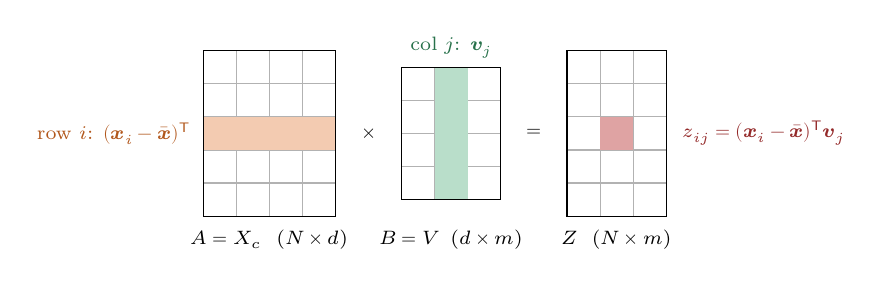
\begin{tikzpicture}[scale=0.42, every node/.style={font=\scriptsize}]
  % A
  \draw[gray!60] (0,0) grid (4,5); \fill[accentC!35] (0,2) rectangle (4,3); \draw (0,0) rectangle (4,5);
  \node at (2,-0.7) {$A=X_c$ \ ($N\times d$)}; \node[accentC!80!black, anchor=east] at (-0.1,2.5) {row $i$: $(\vx_i-\xbar)\T$};
  \node at (5,2.5) {$\times$};
  % B
  \begin{scope}[shift={(6,0.5)}]
  \draw[gray!60] (0,0) grid (3,4); \fill[accentD!35] (1,0) rectangle (2,4); \draw (0,0) rectangle (3,4);
  \node at (1.5,-1.2) {$B=V$ \ ($d\times m$)}; \node[accentD!70!black] at (1.5,4.6) {col $j$: $\vv_j$};
  \end{scope}
  \node at (10,2.5) {$=$};
  % C
  \begin{scope}[shift={(11,0)}]
  \draw[gray!60] (0,0) grid (3,5); \fill[thmred!45] (1,2) rectangle (2,3); \draw (0,0) rectangle (3,5);
  \node at (1.5,-0.7) {$Z$ \ ($N\times m$)}; \node[thmred!80!black, anchor=west] at (3.2,2.5) {$z_{ij}=(\vx_i-\xbar)\T\vv_j$};
  \end{scope}
\end{tikzpicture}
\end{center}

\textbf{PCA scores are exactly this.} The score of point $i$ on PC $j$,
$z_{ij}=(\vx_i-\xbar)\T\vv_j$, answers ``how much of the centered point lies along this direction?'' (Section~\ref{sec:threeways}). Stacking
all points and all directions gives $Z=X_cV$: one dot product per (point, direction) pair.

\textbf{Kernel PCA keeps the same operation,} $z_{0j}=\langle\varphi(\vx_0)-\bar\varphi,\ \vv_j\rangle$, but neither vector is
available. Since $\vv_j$ is a combination of centered training feature vectors, that one dot product expands into
dot products \emph{between feature vectors}, which the kernel supplies (the algorithm in Section~\ref{sec:kpca-alg}).

\textbf{Not every step is a dot product,} since PCA also subtracts, averages, normalizes and eigendecomposes. But the
\emph{geometric information} PCA uses all comes from dot products:
\begin{center}
\renewcommand{\arraystretch}{1.25}
\begin{tabular}{@{}ll@{}}
\toprule
PCA ingredient & in dot products \\ \midrule
centering & subtract the average (no dot product) \\
covariance $\frac1N X_c\T X_c$ / Gram matrix $X_cX_c\T$ & tables of dot products \\
scores $z_{ij}$ & dot product with a PC direction \\
variance along $\vv$ & $\frac1N\sum_i\big((\vx_i-\xbar)\T\vv\big)^2$: average squared dot product \\
\bottomrule
\end{tabular}
\end{center}
That is why a kernel is \emph{enough} for PCA: it hands you every dot product in the hidden feature space.
\end{intuition}

\begin{careful}
\textbf{The kernel matrix does not ``cover every nonlinearity''.} The \emph{kernel} decides which features exist:
$(\vx\T\bm z)^2$ means exactly the degree-$2$ monomials and nothing else. If the true structure involves $x_1^3$ or $\sin x_1$,
that kernel cannot see it. The \emph{kernel matrix} $K$ only evaluates that one kernel on every pair of your data
points. It adds no new features. To cover more, choose a richer kernel: $(c+\vx\T\bm z)^h$ for all degrees $\le h$, or RBF, whose
features include polynomial terms of every degree. Richer kernels are more flexible but overfit more easily and need
tuning (cross-validation, Section~\ref{sec:preimage}). For the circle, even $(\vx\T\bm z)^2$ suffices, since $x_1^2+x_2^2=1$ is
$f_1+f_3=1$ in its features $(x_1^2,\sqrt2x_1x_2,x_2^2)$.
\end{careful}

\begin{example}{The kernel trick is just algebra: a $1$D$\to3$D feature map}{affinekernel}
Map a number $x\in\R$ into $\R^3$ by $\varphi(x)=(x,\ x+1,\ x+2)$, so $\varphi(56)=(56,57,58)$. The kernel is the
inner product of two feature vectors, and plain expansion gives a closed form:
\[
\begin{aligned}
k(x,y)=\langle\varphi(x),\varphi(y)\rangle&=xy+(x+1)(y+1)+(x+2)(y+2)\\
&=xy+(xy+x+y+1)+(xy+2x+2y+4)=\boxed{3xy+3x+3y+5.}
\end{aligned}
\]
Check with $x=1$, $y=2$: through the features, $(1,2,3)\cdot(2,3,4)=2+6+12=20$; through the formula, $6+3+6+5=20$.
The formula never builds a 3-vector. That is the whole trick: expand $\langle\varphi(x),\varphi(y)\rangle$ once, by hand,
and evaluate the short expression from then on. The polynomial and RBF kernels (Examples~\ref{ex:polyk} and~\ref{ex:rbf}) are
the same move with messier algebra.
\end{example}

\begin{careful}
\textbf{An infinite feature map needs its coordinates to shrink.} It is tempting to say that
$\varphi(x)=(x,\ x+\tfrac12,\ x+\tfrac14,\ x+\tfrac18,\dots)$ also has an easy closed form. It does not:
\[
\langle\varphi(x),\varphi(y)\rangle=\sum_{n\ge0}\big(x+2^{-n}\big)\big(y+2^{-n}\big)
=\sum_{n\ge0}\Big(xy+(x+y)2^{-n}+4^{-n}\Big),
\]
and the $xy$ term is added infinitely often, so the sum diverges whenever $xy\ne0$. An inner product in an infinite-dimensional
space needs $\sum_n\varphi_n(x)^2<\infty$. Weighted coordinates fix this. With $\varphi_n(x)=x^n/\sqrt{n!}$ for $n=0,1,2,\dots$,
\[
k(x,y)=\sum_{n\ge0}\frac{(xy)^n}{n!}=e^{xy},
\]
an infinite-dimensional map with a one-line kernel. The RBF kernel is this series multiplied by $e^{-x^2}e^{-y^2}$ (with $\sigma^2=1$, after rescaling $x$ by $\sqrt2$).
\end{careful}

\begin{intuition}
\textbf{Three coordinates, but a line, and not the only map.} All three coordinates of $\varphi(x)=(x,x+1,x+2)$ are
affine in $x$, so the points $\varphi(x)$ lie on a single line in $\R^3$. The kernel adds no curvature: kernel PCA with
it finds one nonzero PC, the same as ordinary PCA on $x$. The feature map is also not unique. Since
$3xy+3x+3y+5=3(x+1)(y+1)+2$, the 2D map $\psi(x)=(\sqrt3\,(x+1),\ \sqrt2)$ gives exactly the same kernel. The kernel fixes the
geometry (every inner product, so every distance and angle) but not the coordinates used to write it down. Theorem~\ref{thm:rkhs} below
says what \emph{is} unique.
\end{intuition}

\begin{intuition}
\textbf{``Pairwise similarity''.} $K_{ij}=k(\vx_i,\vx_j)$ is one number per \emph{pair} of points, and the $N\times N$ matrix $K$ is a
table of how alike every pair is, just as MDS starts from a table of how far apart they are. For an inner product,
$\langle\varphi_i,\varphi_j\rangle=\norm{\varphi_i}\norm{\varphi_j}\cos\theta_{ij}$, so it is large when the feature vectors point the same way. For RBF,
$K_{ij}=e^{-\norm{\vx_i-\vx_j}^2/\sigma^2}\in(0,1]$: $1$ for identical points, near $0$ for far-apart points. With points $0,1,5$ on a line and
$\sigma=1$: $K_{12}=e^{-1}\approx0.37$, while $K_{13}=e^{-25}\approx0$ and $K_{23}=e^{-16}\approx0$. Similarity and distance carry the same information,
$\norm{\varphi_i-\varphi_j}^2=K_{ii}+K_{jj}-2K_{ij}$, and kernel PCA uses nothing but this table.
\end{intuition}

\begin{proposition}{Centering in feature space using only $k$}{centerk}
\[
\widetilde K_{ij}=\langle\tilde\varphi_i,\tilde\varphi_j\rangle
=K_{ij}-\tfrac1N\textstyle\sum_{l}K_{il}-\tfrac1N\sum_{l}K_{lj}+\tfrac1{N^2}\sum_{l,m}K_{lm},
\]
which is exactly the $(i,j)$ entry of $HKH$.
\end{proposition}
\begin{proofsketch}
Expand $\langle\varphi_i-\bar{\varphi},\varphi_j-\bar{\varphi}\rangle
=\langle\varphi_i,\varphi_j\rangle-\langle\varphi_i,\bar{\varphi}\rangle-\langle\bar{\varphi},\varphi_j\rangle+\langle\bar{\varphi},\bar{\varphi}\rangle$
and substitute $\bar{\varphi}=\tfrac1N\sum_l\varphi_l$. Each inner product becomes an average of
kernel values. This is the same double-centering as $B=HAH$ in classical scaling.
\end{proofsketch}

\begin{theorem}{Kernel PC scores are scaled eigenvectors of $\widetilde K$}{kscores}
Let $\vw$ be a unit-length eigenvector of $\Sig_\varphi$ with eigenvalue $\lambda>0$, and let
$\bm z=\widetilde\Phi\vw\in\R^N$ be its score vector, $z_i=\vw\T\tilde\varphi_i$. Then
\begin{enumerate}[nosep,label=(\roman*)]
\item $\widetilde K\bm z=(N\lambda)\,\bm z$: the score vector is an eigenvector of $\widetilde K$ with eigenvalue $\mu=N\lambda$;
\item $\norm{\bm z}^2=N\lambda=\mu$, so $\bm z=\sqrt{\mu}\,\vu$ where $\vu$ is the \emph{unit} eigenvector of $\widetilde K$;
\item the loading itself is $\vw=\tfrac1{\sqrt\mu}\widetilde\Phi\T\vu=\sum_i\tfrac{u_i}{\sqrt\mu}\tilde\varphi_i$, a combination of the centered data features.
\end{enumerate}
\end{theorem}
\begin{proofsketch}
(i) $\Sig_\varphi\vw=\lambda\vw$ means $\tfrac1N\widetilde\Phi\T\widetilde\Phi\vw=\lambda\vw$. Multiply on the left by $\widetilde\Phi$:
$\widetilde\Phi\widetilde\Phi\T(\widetilde\Phi\vw)=N\lambda(\widetilde\Phi\vw)$, i.e.\ $\widetilde K\bm z=N\lambda\bm z$.
(ii) $\norm{\bm z}^2=\vw\T\widetilde\Phi\T\widetilde\Phi\vw=N\vw\T\Sig_\varphi\vw=N\lambda\norm{\vw}^2=N\lambda$.
(iii) From $\Sig_\varphi\vw=\lambda\vw$, $\vw=\tfrac1{N\lambda}\widetilde\Phi\T(\widetilde\Phi\vw)=\tfrac1{\mu}\widetilde\Phi\T\bm z=\tfrac1{\sqrt\mu}\widetilde\Phi\T\vu$.
\end{proofsketch}

\begin{intuition}
Part (iii) is why the trick works even when $D=\infty$. Every loading with $\lambda>0$
lives in the span of the $N$ centered data features, so it is described by $N$ numbers
(the vector $\vu/\sqrt\mu$) instead of $D$ coordinates. The giant $D\times D$ problem and
the small $N\times N$ problem share their nonzero eigenvalues ($\mu=N\lambda$), exactly as
$X\T X$ and $XX\T$ did in Section~\ref{sec:gram}.
\end{intuition}

\begin{careful}
\textbf{Normalization slip.} It is tempting to take a \emph{unit} eigenvector $\bm\alpha$ of
$\widetilde K$, set $\vw=\widetilde\Phi\T\bm\alpha$, and conclude that the scores are
$\widetilde K\bm\alpha=\mu\bm\alpha$. But then $\norm{\vw}^2=\bm\alpha\T\widetilde K\bm\alpha=\mu\neq1$,
so $\vw$ is not a unit loading and the scores come out $\sqrt\mu$ times too large. Rescale
$\bm\alpha\to\bm\alpha/\sqrt\mu$. The correct scores are $\sqrt{\mu}\,\vu$, not $\mu\,\vu$.
\end{careful}

\begin{proposition}{At most $N-1$ kernel PCs, even if $D=\infty$}{kNminus1}
$\sum_{i=1}^N\tilde\varphi_i=\bm 0$. So $\tilde\varphi_1,\dots,\tilde\varphi_N$ are linearly
dependent and span a linear subspace of $\mathcal F$ of dimension at most $N-1$. Equivalently,
the features $\varphi(\vx_i)=\tilde\varphi_i+\bar{\varphi}$ lie in an affine subspace of dimension at most $N-1$.
Hence $\rank\widetilde K\le N-1$, and at most $N-1$ kernel PC variances are nonzero.
\end{proposition}
\begin{proofsketch}
$\sum_i\tilde\varphi_i=\sum_i\varphi(\vx_i)-N\bar{\varphi}=\bm0$ by the definition of $\bar{\varphi}$. A
nontrivial combination equal to zero is the definition of linear dependence. This is the same argument
as Prop.~\ref{prop:nminus1}, now in a space that may have infinitely many coordinates.
Directly, $\widetilde K\one=HKH\one=\bm0$ because $H\one=\bm0$.

\emph{A second proof by anchoring.} Pick $\varphi(\vx_1)$ as an anchor and form the $N-1$ difference
vectors $\bm d_i=\varphi(\vx_i)-\varphi(\vx_1)$, $i=2,\dots,N$. Their span $S$ has dimension at most $N-1$,
and every point is $\varphi(\vx_i)=\varphi(\vx_1)+\bm d_i\in\varphi(\vx_1)+S$, an affine subspace of dimension
$\le N-1$. Sliding the anchor to the origin changes no pairwise distance. So 3 points need at most a
plane, 4 points at most 3D (a tetrahedron), and in general $N$ points never need more than $N-1$
dimensions, \emph{however} large the ambient space. They may need fewer, e.g.\ $1$ if they are collinear.
\end{proofsketch}

\begin{intuition}
This is why the $N\times N$ route is not just cheaper but \emph{sufficient}. With $N>d$ in
ordinary PCA you would diagonalize the $d\times d$ matrix $(HX)\T(HX)$. In feature space
$D$ may be $\infty$, but the data occupy at most $N-1$ dimensions of it, and $\widetilde K$
captures all of them.
\end{intuition}

\subsection{Which functions are kernels? Mercer's condition}

Not every function of two points is an inner product of features. We need a test that uses
only $k$.

\textbf{Why symmetric?} An inner product is symmetric, $\langle\varphi(\vx),\varphi(\vy)\rangle=\langle\varphi(\vy),\varphi(\vx)\rangle$,
so a kernel must satisfy $k(\vx,\vy)=k(\vy,\vx)$. In matrix terms, $K$ is then a symmetric
matrix, and the spectral theorem (Theorem~\ref{thm:spectral}) guarantees that $\widetilde K=HKH$ has
real eigenvalues and orthonormal eigenvectors. Without symmetry the eigendecomposition step of
the algorithm would not make sense. Symmetry is necessary but not enough: we also need
$K$ to be PSD.

\begin{definition}{Mercer's condition}{mercer}
A symmetric function $k:\R^d\times\R^d\to\R$ (meaning $k(\vx,\vy)=k(\vy,\vx)$) \textbf{satisfies Mercer's
condition} if for every $N\in\{1,2,\dots\}$ and every choice of points $\vx_1,\dots,\vx_N\in\R^d$, the
kernel matrix $K\in\R^{N\times N}$ with $K_{ij}=k(\vx_i,\vx_j)$ is positive semidefinite.
\end{definition}
Such a $k$ is also called a \textbf{positive semidefinite (PSD) function} or
\textbf{positive definite kernel}. So ``kernel'', ``Mercer kernel'' and ``PSD function'' name the
same thing: a function whose every kernel matrix is a PSD matrix.

\begin{theorem}{Mercer kernels are exactly inner products of features}{mercerfeat}
\begin{enumerate}[nosep,label=(\alph*)]
\item If $k(\vx,\vy)=\langle\varphi(\vx),\varphi(\vy)\rangle_{\mathcal F}$ for some feature map $\varphi$, then $k$ satisfies Mercer's condition.
\item Conversely, if $k$ satisfies Mercer's condition, then there exist a feature space $\mathcal F$ (an
inner-product space, possibly infinite-dimensional) and a map $\varphi:\R^d\to\mathcal F$ with
\[
k(\vx,\vy)=\langle\varphi(\vx),\varphi(\vy)\rangle_{\mathcal F}\ \big(=\varphi(\vx)\T\varphi(\vy)\ \text{when }\mathcal F=\R^D\big).
\]
\end{enumerate}
\end{theorem}
\begin{proofsketch}
(a) For any $\bm v\in\R^N$,
$\bm v\T K\bm v=\sum_{i,j}v_iv_j\langle\varphi(\vx_i),\varphi(\vx_j)\rangle=\big\|\sum_iv_i\varphi(\vx_i)\big\|^2\ge0$.
(b) This direction is the deep one, and we take it as given. One explicit construction
appears in Section~\ref{sec:spectral}: the eigenfunctions of $k$ supply the coordinates of
$\varphi$.
\end{proofsketch}

\begin{intuition}
Why kernel PCA needs Mercer's condition: it guarantees $\widetilde K=HKH$ is PSD as well, since
$\bm v\T HKH\bm v=(H\bm v)\T K(H\bm v)\ge0$. So all eigenvalues $\mu_j\ge0$, the square roots
$\sqrt{\mu_j}$ in the scores exist, and the variances $\mu_j/N$ are nonnegative. A function that
fails the condition can produce negative ``variances''. This is the same failure as a
non-Euclidean distance matrix in classical scaling (Theorem~\ref{thm:edm}).
\end{intuition}

\begin{theorem}{Reproducing kernel Hilbert space (Moore--Aronszajn)}{rkhs}
If $k:\mathcal X\times\mathcal X\to\R$ is symmetric and positive definite (Mercer's condition), then there is a
\textbf{unique} Hilbert space $\mathcal H$ of functions $f:\mathcal X\to\R$ for which $k$ is a \textbf{reproducing kernel}:
\begin{enumerate}[nosep,label=(\roman*)]
\item for every $\vx$, the function $k(\cdot,\vx)$ belongs to $\mathcal H$;
\item for every $f\in\mathcal H$ and every $\vx$, $\ f(\vx)=\langle f,\,k(\cdot,\vx)\rangle_{\mathcal H}$ (the \emph{reproducing property}).
\end{enumerate}
Taking $f=k(\cdot,\vy)$ in (ii) gives $k(\vx,\vy)=\langle k(\cdot,\vx),k(\cdot,\vy)\rangle_{\mathcal H}$. So
$\varphi(\vx)=k(\cdot,\vx)$ is a feature map for $k$, and $\mathcal H$ is its feature space.
\end{theorem}

\begin{intuition}
\textbf{This is the licence for the kernel trick.} The theorem gives the conditions under which a function $k$ can stand
in for $\langle\varphi(\vx),\varphi(\vy)\rangle$ without ever computing $\varphi$: if $k$ is symmetric positive definite, some feature space
exists, so every formula written in inner products (PCA scores, distances, centering) means something there. In the RKHS the
feature of a point is a whole \emph{function}, the bump $k(\cdot,\vx)$ centred at $\vx$, and an inner product with that bump
evaluates a function at $\vx$.

\textbf{What is unique and what is not.} The Hilbert space $\mathcal H$ of functions is unique. Coordinate feature maps into
$\R^D$ are not: the previous Intuition gave two different maps, into $\R^3$ and $\R^2$, for $3xy+3x+3y+5$. Both are just ways of
writing down coordinates for the same $\mathcal H$.
\end{intuition}

\begin{careful}
\textbf{You cannot pick any $k$ and use it willy-nilly.} Check that a kernel is symmetric and PSD before using it. Building $k$
from a feature map, as in Example~\ref{ex:affinekernel}, always passes (Theorem~\ref{thm:mercerfeat}(a)). Writing down a similarity formula
directly does not: $\norm{\vx-\vy}^2$ below fails, and so does the sigmoid kernel $\tanh(a\,\vx\T\vy+c)$ for many $a,c$. With an invalid
$k$ there is no feature space behind the numbers, $\widetilde K$ can have negative eigenvalues, and kernel PCA returns negative ``variances''
and imaginary scores $\sqrt{\mu_j}$. \textbf{Terminology:} ``positive definite kernel'' means every kernel matrix is PSD
(Definition~\ref{def:mercer}), not that every kernel matrix is strictly positive definite.
\end{careful}

\begin{example}{Kernels and a non-kernel}{kernelcheck}
\begin{itemize}[nosep]
\item $k(\vx,\vy)=(1+\vx\T\vy)^2$ and the RBF kernel are Mercer kernels. Both have explicit feature maps (Examples below), so part (a) applies.
\item Sums and positive multiples of Mercer kernels are Mercer kernels: $\bm v\T(K_1+K_2)\bm v=\bm v\T K_1\bm v+\bm v\T K_2\bm v\ge0$. Products are too, by the Schur product theorem (the entrywise product of two PSD matrices is PSD).
\item $k(\vx,\vy)=\norm{\vx-\vy}^2$ is \textbf{not} a Mercer kernel. Take two distinct points: $K=\begin{bmatrix}0&c\\c&0\end{bmatrix}$ with $c>0$, whose eigenvalues are $\pm c$, so one is negative. A squared distance measures \emph{dissimilarity}, and a kernel must measure \emph{similarity}.
\end{itemize}
\end{example}

\begin{example}{Polynomial kernel}{polyk}
For $\vx,\vy\in\R^2$, $k(\vx,\vy)=(c+\vx\T\vy)^2=\varphi(\vx)\T\varphi(\vy)$ with
\[
\varphi(\vx)=\big(c,\ \sqrt{2c}\,x_1,\ \sqrt{2c}\,x_2,\ x_1^2,\ x_2^2,\ \sqrt2\,x_1x_2\big).
\]
Check: $(c+x_1y_1+x_2y_2)^2=c^2+2cx_1y_1+2cx_2y_2+x_1^2y_1^2+x_2^2y_2^2+2x_1x_2y_1y_2$.
One dot product and one square stand in for a 6-dimensional feature map. The $\sqrt2$'s are not
decoration: they are exactly what makes the cross terms match.
\end{example}

\begin{example}{RBF / Gaussian kernel: an infinite-dimensional feature map}{rbf}
\[
k(\vx,\vy)=e^{-\norm{\vx-\vy}^2/\sigma^2}
=e^{-\norm{\vx}^2/\sigma^2}\,e^{-\norm{\vy}^2/\sigma^2}\,e^{2\vx\T\vy/\sigma^2}
=\sum_{\ell=0}^{\infty}e^{-\norm{\vx}^2/\sigma^2}e^{-\norm{\vy}^2/\sigma^2}\frac{1}{\ell!}\Big(\frac{2\vx\T\vy}{\sigma^2}\Big)^{\ell}.
\]
Each power $(\vx\T\vy)^\ell$ expands into all monomials of degree $\ell$. So the implicit
$\varphi(\vx)$ is $e^{-\norm{\vx}^2/\sigma^2}$ times \emph{all polynomial terms of all
degrees} in the coordinates of $\vx$, which is an \textbf{infinite-dimensional feature map}.
Yet $k$ costs one distance computation. Locally,
$k\approx1-\tfrac{\norm{\vx-\vy}^2}{\sigma^2}+\tfrac{\norm{\vx-\vy}^4}{2\sigma^4}-\cdots$,
so $\sigma$ sets the length scale at which points count as ``similar''.
\end{example}

\begin{example}{Tiny bandwidth: $\sigma^2\to0$ makes $K\to I_N$}{rbfsmall}
For distinct points, $k(\vx_i,\vx_j)=e^{-\norm{\vx_i-\vx_j}^2/\sigma^2}\to0$ as $\sigma^2\to0$ (any fixed positive distance divided by a vanishing $\sigma^2$
blows up), while $k(\vx_i,\vx_i)=e^0=1$ always. So for three distinct points
\[
K=\begin{bmatrix}k(\vx_1,\vx_1)&k(\vx_1,\vx_2)&k(\vx_1,\vx_3)\\k(\vx_2,\vx_1)&k(\vx_2,\vx_2)&k(\vx_2,\vx_3)\\k(\vx_3,\vx_1)&k(\vx_3,\vx_2)&k(\vx_3,\vx_3)\end{bmatrix}
\ \longrightarrow\ \begin{bmatrix}1&0&0\\0&1&0\\0&0&1\end{bmatrix}=I_3 .
\]
\textbf{Reading the identity.} $K_{ii}=1$: every point is perfectly similar to itself. $K_{ij}=0$ for $i\ne j$: every distinct pair has zero
similarity. Since $K_{ij}=\langle\psi(\vx_i),\psi(\vx_j)\rangle$ (Fact~\ref{kf:innerprod}), all the feature vectors are \textbf{unit length and mutually
perpendicular}, like the standard basis $\bm e_1,\bm e_2,\bm e_3$. The kernel is saying ``each distinct training point is its own
completely unrelated thing''.

\textbf{Where the $\sqrt2$ comes from.} The points are \emph{not} at distance $0$. With $\bm a=\psi(\vx_i)$, $\bm b=\psi(\vx_j)$ and $i\ne j$:
\[
\norm{\bm a-\bm b}^2=\norm{\bm a}^2+\norm{\bm b}^2-2\langle\bm a,\bm b\rangle=1+1-2\cdot0=2,\qquad \norm{\psi(\vx_i)-\psi(\vx_j)}=\sqrt2 .
\]
Picture $\bm a=(1,0)$ and $\bm b=(0,1)$: the segment between their tips is the hypotenuse of a $1$-by-$1$ right triangle, of length $\sqrt{1^2+1^2}$.

\textbf{Each point gets its own axis.} With three points, the feature vectors become the three standard basis vectors
$\bm e_1,\bm e_2,\bm e_3$, and their tips form an equilateral triangle with side $\sqrt2$. With $N$ points it is the same thing in
$N$ dimensions: the tips are the corners of a regular simplex. Every point is equally far from every other point, so the
feature space forgets everything about which points were close in the original space. The kernel is so narrow that each
point only ``sees'' itself.
\begin{center}
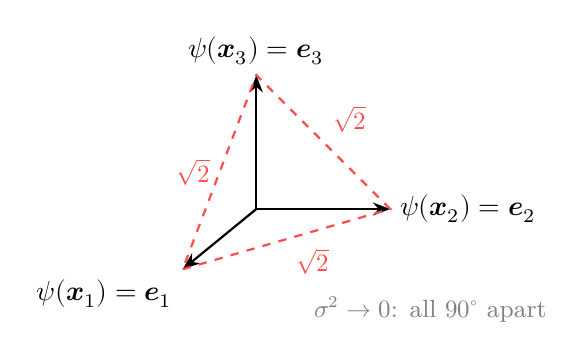
\begin{tikzpicture}[scale=1.7,>={Stealth[length=2.2mm]},x={(-0.55cm,-0.45cm)},y={(1cm,0cm)},z={(0cm,1cm)}]
  \draw[->,thick] (0,0,0) -- (1,0,0) node[below left] {$\psi(\vx_1)=\bm e_1$};
  \draw[->,thick] (0,0,0) -- (0,1,0) node[right] {$\psi(\vx_2)=\bm e_2$};
  \draw[->,thick] (0,0,0) -- (0,0,1) node[above] {$\psi(\vx_3)=\bm e_3$};
  \draw[red!70,dashed,thick] (1,0,0) -- (0,1,0) -- (0,0,1) -- cycle;
  \node[red!70,font=\small] at (0.5,0.5,0) [below right] {$\sqrt2$};
  \node[red!70,font=\small] at (0,0.5,0.5) [above right] {$\sqrt2$};
  \node[red!70,font=\small] at (0.5,0,0.5) [left] {$\sqrt2$};
  \node[font=\small,gray] at (0,1.3,-0.75) {$\sigma^2\to0$: all $90^\circ$ apart};
\end{tikzpicture}
\end{center}
\end{example}

\begin{example}{Distances from kernel values, and back to the original space}{kdist}
\textbf{Feature-space distance from $K$.} Let $\bm a=\psi(\vx_i)$, $\bm b=\psi(\vx_j)$. A squared length is a vector dotted with itself, so expand
$\langle\bm a-\bm b,\bm a-\bm b\rangle$ exactly like $(a-b)^2$:
\[
\norm{\bm a-\bm b}^2=\langle\bm a,\bm a\rangle-\langle\bm a,\bm b\rangle-\langle\bm b,\bm a\rangle+\langle\bm b,\bm b\rangle=\langle\bm a,\bm a\rangle+\langle\bm b,\bm b\rangle-2\langle\bm a,\bm b\rangle,
\]
using symmetry, $\langle\bm a,\bm b\rangle=\langle\bm b,\bm a\rangle$. Each inner product is a kernel entry: $\langle\psi(\vx_i),\psi(\vx_i)\rangle=K_{ii}$, $\langle\psi(\vx_j),\psi(\vx_j)\rangle=K_{jj}$, $\langle\psi(\vx_i),\psi(\vx_j)\rangle=K_{ij}$. So
\[
\boxed{\ \norm{\psi(\vx_i)-\psi(\vx_j)}=\sqrt{K_{ii}+K_{jj}-2K_{ij}}\ }\qquad\overset{\text{RBF: }K_{ii}=K_{jj}=1}{\Longrightarrow}\qquad \norm{\psi(\vx_i)-\psi(\vx_j)}=\sqrt{2-2K_{ij}} .
\]
\textbf{Why the minus sign.} It is the ordinary geometry of the law of cosines: two vectors that point the same way have a
large inner product, and subtracting it makes their distance small. RBF checks: identical points, $K_{ij}=1$, give $\sqrt{2-2}=0$;
orthogonal feature vectors, $K_{ij}=0$, give $\sqrt2$ (Example~\ref{ex:rbfsmall}). The quantity under the root is never negative, since it
is a squared length (for a valid kernel, $K_{ii}+K_{jj}-2K_{ij}=(\bm e_i-\bm e_j)\T K(\bm e_i-\bm e_j)\ge0$ by PSD).

\textbf{Recovering the original-space distance (RBF only).} Invert the kernel's definition. Take logs of $K_{ij}=\exp\!\big(-\norm{\vx_i-\vx_j}^2/\sigma^2\big)$:
\[
\ln K_{ij}=-\frac{\norm{\vx_i-\vx_j}^2}{\sigma^2}\ \Longrightarrow\ \norm{\vx_i-\vx_j}^2=-\sigma^2\ln K_{ij}\ \Longrightarrow\ \boxed{\ \norm{\vx_i-\vx_j}=\sigma\sqrt{-\ln K_{ij}}\ } .
\]
The minus sign makes the root legal: RBF values satisfy $0<K_{ij}\le1$, so $\ln K_{ij}\le0$ and $-\ln K_{ij}\ge0$. Example: $K_{ij}=e^{-4}$ and $\sigma=2$ give
$\norm{\vx_i-\vx_j}=2\sqrt{-\ln e^{-4}}=2\sqrt4=4$.
\end{example}

\begin{intuition}
\textbf{Two distances, one kernel value.} Combining the boxes, for RBF the feature-space distance is a fixed function of
the input distance $r=\norm{\vx_i-\vx_j}$:
\[
\norm{\psi(\vx_i)-\psi(\vx_j)}=\sqrt{2-2e^{-r^2/\sigma^2}} .
\]
It grows with $r$, so near points stay near and far points stay far, but it \emph{saturates} at $\sqrt2$: every pair farther than a few
$\sigma$ apart looks equally far in feature space. This is the ``neighborhood detector'' picture explained below. The RBF map keeps local
geometry and forgets how far apart distant points are.
\end{intuition}

\begin{careful}
The inversion works only because you know the kernel \emph{is} RBF and know $\sigma$. From a kernel matrix alone, with an
unknown kernel, you can always recover distances in that kernel's \emph{feature space} (the first box), but not
necessarily the original-space distances.
\end{careful}

\subsubsection*{The kernel picks a similarity; distance comes with it}

A kernel is a chosen \emph{similarity} (inner-product) formula, not fundamentally a distance formula. For any valid
(PSD) kernel there is a feature map with $k(\vx,\bm y)=\langle\varphi(\vx),\varphi(\bm y)\rangle$, and the feature-space distance it implies is always
\[
D_{ij}^2=k(\vx_i,\vx_i)+k(\vx_j,\vx_j)-2k(\vx_i,\vx_j)\qquad(\text{Example~\ref{ex:kdist}}).
\]
Different kernels make different design choices:
\begin{itemize}[nosep]
\item \textbf{Linear}, $k(\vx,\bm y)=\vx\T\bm y$: $\varphi(\vx)=\vx$, so $D_{ij}=\norm{\vx_i-\vx_j}$, ordinary Euclidean distance. Feature vectors have varying lengths and
distances are unbounded.
\item \textbf{RBF}, $k=e^{-\norm{\vx-\bm y}^2/\sigma^2}$: similarity decays with distance and $k(\vx,\vx)=1$, so
$D_{ij}=\big(2-2e^{-\norm{\vx_i-\vx_j}^2/\sigma^2}\big)^{1/2}$, capped at $\sqrt2$.
\end{itemize}

\begin{proposition}{RBF feature vectors live on the unit sphere}{rbfsphere}
For the RBF kernel, $\norm{\varphi(\vx)}=1$ for every $\vx$, and with $\theta_{ij}$ the angle between $\varphi(\vx_i)$ and $\varphi(\vx_j)$,
\[
K_{ij}=\cos\theta_{ij},\qquad D_{ij}=\sqrt{2-2\cos\theta_{ij}},\qquad 0^\circ\le\theta_{ij}<90^\circ\ \ (\text{since }K_{ij}>0).
\]
\end{proposition}
\begin{proofsketch}
A squared length is a vector's inner product with itself, so $\norm{\varphi(\vx)}^2=\langle\varphi(\vx),\varphi(\vx)\rangle=k(\vx,\vx)=e^{-0}=1$. ``All vectors of length $1$'' is the
definition of the unit sphere $\{\bm v:\norm{\bm v}=1\}$. Then $\langle\bm a,\bm b\rangle=\norm{\bm a}\norm{\bm b}\cos\theta=\cos\theta$ (Fact~\ref{kf:innerprod}).
\end{proofsketch}

\begin{careful}
The \emph{original} points $\vx$ do not lie on a sphere; their hidden representations $\varphi(\vx)$ do. And $D_{ij}=\norm{\varphi(\vx_i)-\varphi(\vx_j)}$ is the
\textbf{straight-line chord} through feature space, not the distance along the sphere's surface. The geodesic (arc) distance on
the unit sphere would be the angle itself, $\theta_{ij}=\arccos K_{ij}$. The two agree for small angles ($2-2\cos\theta\approx\theta^2$) and differ at
$90^\circ$: chord $\sqrt2\approx1.41$ vs.\ arc $\pi/2\approx1.57$.
\end{careful}

\begin{figure}[htbp]
\centering
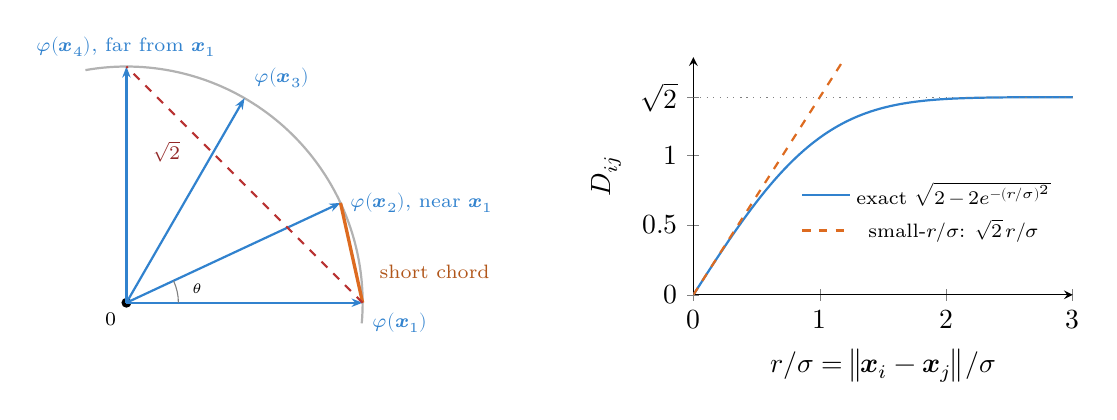
\begin{tikzpicture}
\begin{scope}[scale=3.0]
  \draw[gray!60, thick] (0,0) ++(-5:1) arc (-5:100:1);
  \fill (0,0) circle (0.6pt) node[below left, font=\scriptsize] {$\bm0$};
  \coordinate (A) at (0:1); \coordinate (B) at (25:1); \coordinate (C) at (60:1); \coordinate (E) at (90:1);
  \draw[-{Stealth[length=4pt]}, thick, dataC] (0,0) -- (A) node[below right, font=\scriptsize] {$\varphi(\vx_1)$};
  \draw[-{Stealth[length=4pt]}, thick, dataC] (0,0) -- (B) node[right, font=\scriptsize] {$\varphi(\vx_2)$, near $\vx_1$};
  \draw[-{Stealth[length=4pt]}, thick, dataC] (0,0) -- (C) node[above right, font=\scriptsize] {$\varphi(\vx_3)$};
  \draw[-{Stealth[length=4pt]}, thick, dataC] (0,0) -- (E) node[above, font=\scriptsize] {$\varphi(\vx_4)$, far from $\vx_1$};
  \draw[very thick, accentC] (A) -- (B);
  \draw[thick, thmred, dashed] (A) -- (E);
  \node[thmred!80!black, font=\scriptsize] at (0.17,0.64) {$\sqrt2$};
  \draw[gray] (0.22,0) arc (0:25:0.22); \node[font=\tiny] at (0.3,0.06) {$\theta$};
  \node[font=\scriptsize, accentC!80!black, anchor=west] at (1.03,0.13) {short chord};
\end{scope}
\begin{axis}[xshift=7.2cm, yshift=0.1cm, width=6.4cm, height=4.6cm, axis lines=left, xlabel={$r/\sigma=\norm{\vx_i-\vx_j}/\sigma$}, ylabel={$D_{ij}$},
  xmin=0, xmax=3, ymin=0, ymax=1.7, ytick={0,0.5,1,1.414}, yticklabels={$0$,$0.5$,$1$,$\sqrt2$}, legend style={font=\scriptsize, at={(0.98,0.35)}, anchor=east, draw=none}]
\addplot[thick, dataC, domain=0:3, samples=80] {sqrt(2-2*exp(-x^2))};
\addplot[thick, dashed, accentC, domain=0:1.2] {sqrt(2)*x};
\addplot[thin, gray, dotted, domain=0:3] {sqrt(2)};
\legend{exact $\sqrt{2-2e^{-(r/\sigma)^2}}$, small-$r/\sigma$: $\sqrt2\,r/\sigma$}
\end{axis}
\end{tikzpicture}
\caption{\textbf{Left:} every RBF feature vector has length $1$, so the inputs map to a unit sphere in feature space (an arc shown).
Nearby inputs get a small angle and a short chord; very distant inputs get nearly perpendicular vectors and chord $\sqrt2$.
\textbf{Right:} the chord as a function of $r/\sigma$. It starts out \emph{linear} (distances preserved up to the factor $\sqrt2/\sigma$) and
saturates at $\sqrt2$.}
\end{figure}

\begin{center}
\renewcommand{\arraystretch}{1.3}
\small
\begin{tabular}{@{}lccc@{}}
\toprule
angle between feature vectors & $K_{ij}=\cos\theta$ & $D_{ij}=\sqrt{2-2\cos\theta}$ & meaning \\
\midrule
$0^\circ$ & $1$ & $0$ & same feature point \\
$90^\circ$ & $0$ & $\sqrt2$ & unrelated (orthogonal) \\
$180^\circ$ & $-1$ & $2$ & opposite (never for RBF: $K>0$) \\
\bottomrule
\end{tabular}
\end{center}

\subsubsection*{\texorpdfstring{$\sigma$}{sigma} is a zoom knob: only the ratio $\norm{\vx_i-\vx_j}^2/\sigma^2$ matters}

\begin{center}
\renewcommand{\arraystretch}{1.35}
\small
\begin{tabular}{@{}>{\raggedright\arraybackslash}p{4.0cm}ccc>{\raggedright\arraybackslash}p{4.4cm}@{}}
\toprule
what changes & ratio $\norm{\vx_i-\vx_j}^2/\sigma^2$ & $K_{ij}$ & $D_{ij}$ & meaning \\
\midrule
$\sigma^2\to\infty$, points fixed & $\to0$ & $\to1$ & $\to0$ & all points collapse to one feature point \\
$\norm{\vx_i-\vx_j}\to\infty$, $\sigma$ fixed & $\to\infty$ & $\to0$ & $\to\sqrt2$ & very distant inputs become nearly orthogonal \\
$\sigma^2\to0$, $\vx_i\ne\vx_j$ & $\to\infty$ & $\to0$ & $\to\sqrt2$ & every distinct pair becomes nearly orthogonal \\
\bottomrule
\end{tabular}
\end{center}

\noindent There is no contradiction between $D\to0$ and $D\to\sqrt2$: they are opposite ends of the same ratio. If $\sigma$ dwarfs the separation,
$K\to1$ and $D\to0$; if the separation dwarfs $\sigma$, $K\to0$ and $D\to\sqrt2$. As matrices (three points):
\[
\sigma^2\to\infty:\ K\to\begin{bmatrix}1&1&1\\1&1&1\\1&1&1\end{bmatrix},\ D\to\begin{bmatrix}0&0&0\\0&0&0\\0&0&0\end{bmatrix};
\qquad
\sigma^2\to0:\ K\to I_3,\ D\to\begin{bmatrix}0&\sqrt2&\sqrt2\\\sqrt2&0&\sqrt2\\\sqrt2&\sqrt2&0\end{bmatrix}.
\]
($K$ and $D$ are different matrices: $D$ is computed from $K$ through $D_{ij}^2=K_{ii}+K_{jj}-2K_{ij}$. ``$K$ is all ones'' gives $D_{ij}^2=1+1-2=0$.)

\begin{figure}[htbp]
\centering
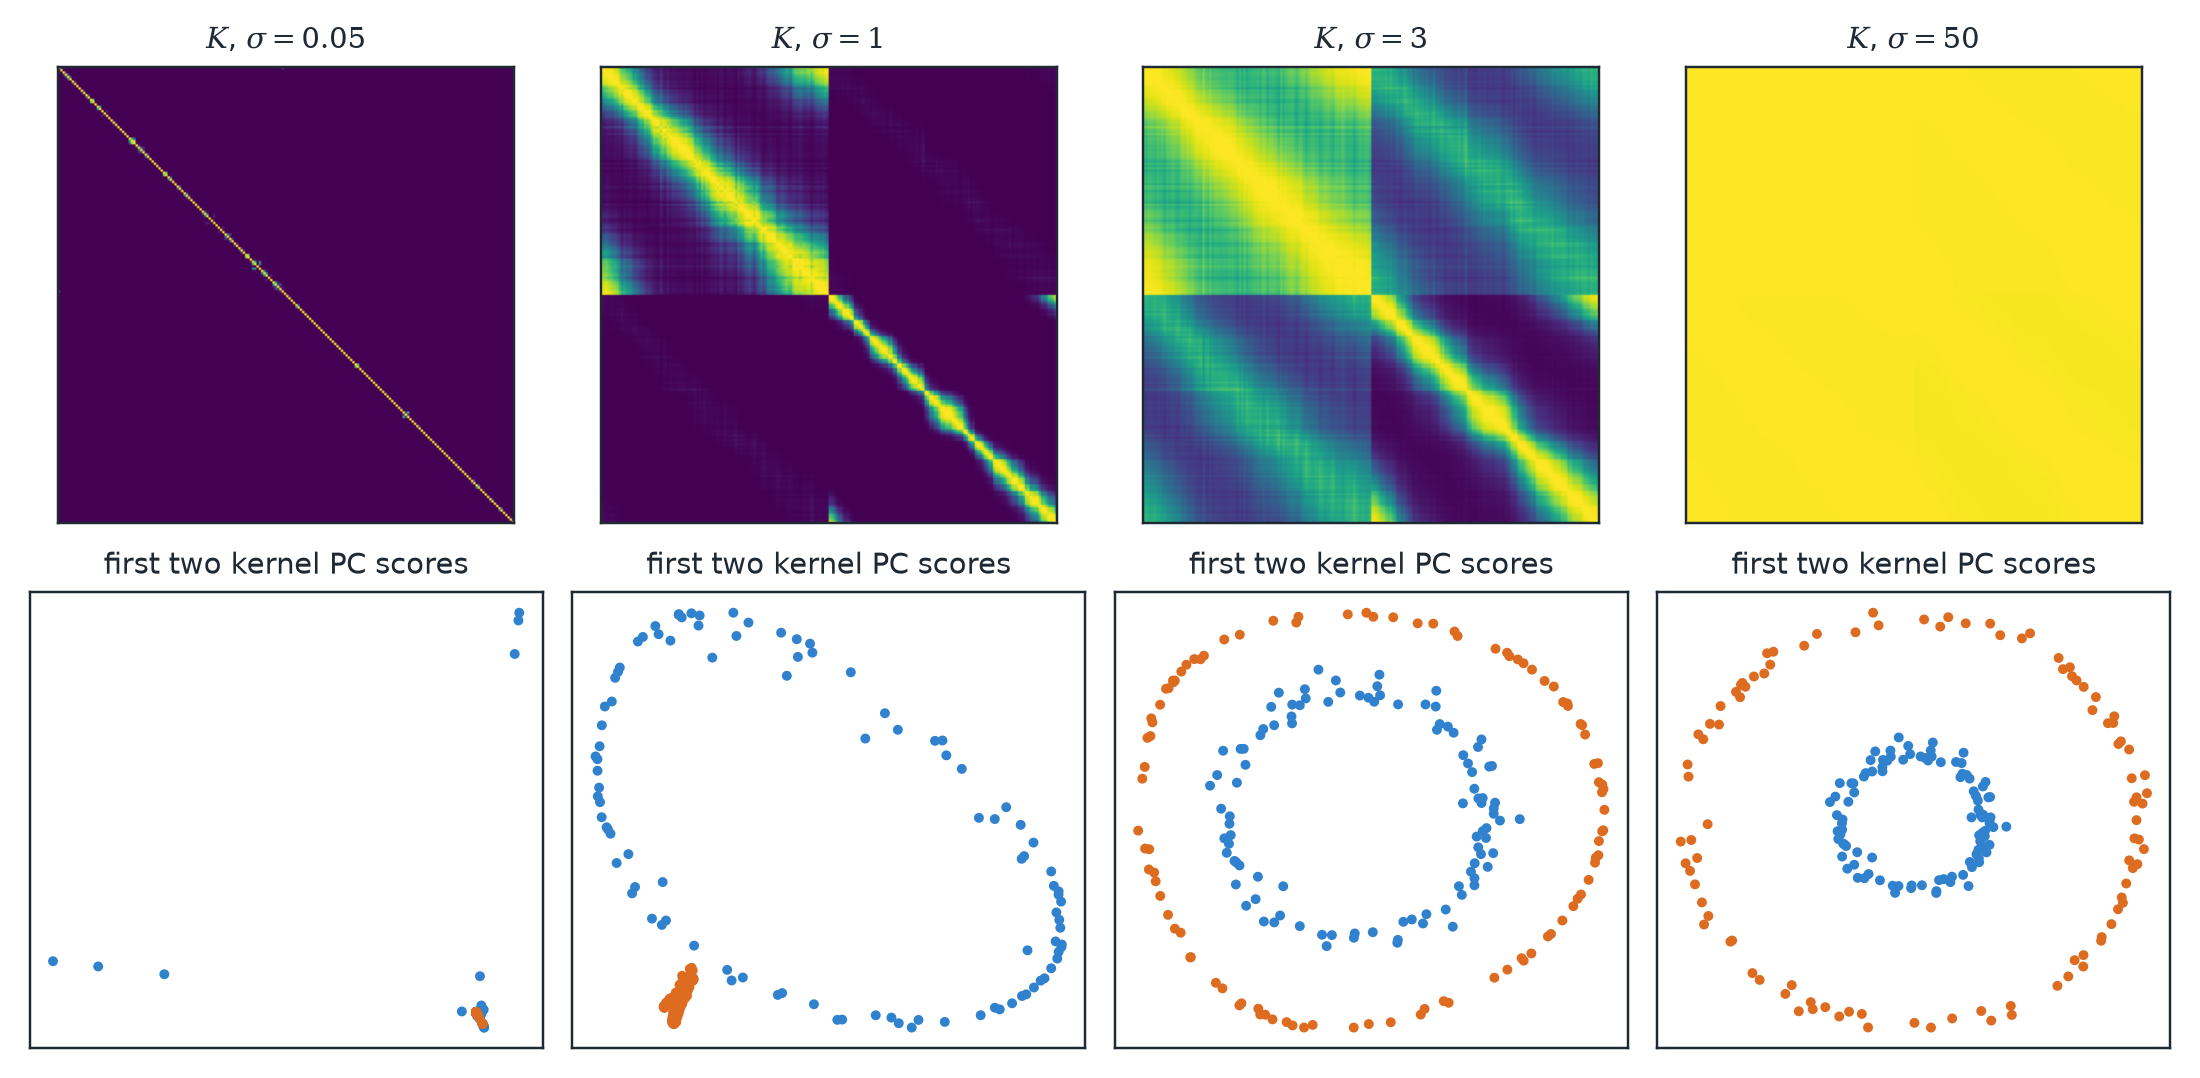
\includegraphics[width=\textwidth]{figures/kpca_sigma.png}
\caption{Kernel PCA with an RBF kernel on two noisy rings (radii $1$ and $3$, $100$ points each; blue is the inner ring). In the heatmaps, points are sorted by ring, then by angle. $\sigma=0.05$: $K\approx I$ (mean off-diagonal entry $0.0009$), every direction carries about $1\%$ of the variance, and the top scores just pick out a few points. $\sigma=1$: similarity is local, and the top two components trace the inner ring while the outer ring collapses. $\sigma=3$: both rings appear. $\sigma=50$: $K\approx\one\one\T$ (mean off-diagonal $0.996$), and the top two components hold $99.7\%$ of the variance and simply reproduce the original picture, as linear PCA would.}
\label{fig:kpcasigma}
\end{figure}

\begin{example}{Large but finite $\sigma$: distances shrink, but proportionally}{largesigma}
Let $t=\norm{\vx_i-\vx_j}^2/\sigma^2$. For $\sigma^2$ large (points fixed), $t$ is small and $e^{-t}\approx1-t$, so
\[
D_{ij}^2=2-2e^{-t}\approx2-2(1-t)=2t=\frac{2\norm{\vx_i-\vx_j}^2}{\sigma^2}
\qquad\Longrightarrow\qquad
\boxed{\,D_{ij}\approx\frac{\sqrt2}{\sigma}\,\norm{\vx_i-\vx_j}\,} .
\]
(The common slip is to drop the $2$ and write $\sqrt{\norm{\vx_i-\vx_j}^2/\sigma^2}$.) Feature distance is then \emph{proportional} to original
distance, so the RBF map approximately preserves the original geometry, shrunk by $\sqrt2/\sigma$. As $\sigma\to\infty$ the factor
$\sqrt2/\sigma\to0$ and every distance goes to $0$: the collapse in the first row of the table, now seen as a limit rather than a
contradiction.
\end{example}

\begin{intuition}
\textbf{The geometric picture.} $\sigma$ answers ``how close counts as similar?''. With a \emph{huge} $\sigma$ every finite separation
looks tiny, so all feature vectors point in nearly the same direction and crowd into one small patch of the sphere. A
small patch of a sphere looks flat (Section~\ref{sec:manifold}), so inside it chord distances are proportional to the
original ones: geometry preserved, but squashed by $\sqrt2/\sigma$. With a \emph{tiny} $\sigma$ even modest separations look
enormous, distinct points get nearly perpendicular vectors, and every pair sits at chord $\sqrt2$: all structure lost.
Useful $\sigma$ sit between, where near points are close on the sphere and far points saturate. That is why kernel PCA with
large $\sigma$ behaves like linear PCA, and with tiny $\sigma$ sees nothing (the Careful box below).
\end{intuition}

\begin{intuition}
\textbf{Does zero similarity mean ``orthogonal'' or ``far apart''? Both, in two different spaces.} For any valid (Mercer)
kernel, $k(\vx,\bm z)=\langle\varphi(\vx),\varphi(\bm z)\rangle$, so $k=0$ \emph{always} means the feature vectors are perpendicular. What that says about the
\emph{original} inputs depends on the kernel:
\begin{itemize}[nosep]
\item \textbf{Linear} $\vx\T\bm z$: the original vectors themselves are perpendicular.
\item \textbf{RBF}: in input space $k\approx0\iff\norm{\vx-\bm z}\gg\sigma$, so the points are far apart \emph{relative to} $\sigma$. In feature space,
the same points are nearly perpendicular. ``Far apart before the map'' becomes ``almost perpendicular after it''.
\item \textbf{Polynomial}: the polynomial-feature vectors are perpendicular, which need not look like ordinary
perpendicularity of $\vx$ and $\bm z$.
\end{itemize}
Two cautions. Perpendicular means ``far'' here only because every RBF feature vector has the same length $1$; in general a
zero inner product says nothing about distance by itself. And for finite $\sigma$ the RBF value is never exactly $0$, only
arbitrarily close, so the exact $K=I$ is a limit. (For an informal ``similarity function'' that is not PSD, a zero has no
feature-space meaning at all.)
\end{intuition}

\begin{intuition}
\textbf{Why ``far apart'' turns into ``perpendicular'': RBF features are neighborhood detectors.} Think of an RBF feature vector
as recording \emph{which neighborhoods a point belongs to}. Two nearby inputs activate many of the same neighborhood
features, so their feature vectors point in similar directions and $\langle\varphi(\vx),\varphi(\bm y)\rangle\approx1$. Two far-apart inputs share
essentially no neighborhoods, their feature vectors have no overlapping components, and the inner product is near $0$,
which is exactly what perpendicular means.

\emph{A finite analogy:} one feature per city, $\varphi(\text{New York})=(1,0,0)$ and $\varphi(\text{Los Angeles})=(0,1,0)$. No active feature in common, so
$\varphi(\text{NY})\T\varphi(\text{LA})=0$: perpendicular.

\emph{The exact version.} Put a Gaussian ``bump sensor'' at every location $\bm c\in\R^d$, and let feature $\bm c$ of a point be how
strongly it triggers that sensor, $\varphi_{\bm c}(\vx)\propto e^{-2\norm{\vx-\bm c}^2/\sigma^2}$. The inner product sums (integrates) over all sensors, and
the integral of a product of two Gaussians is again a Gaussian in the distance between their centers:
\[
\int e^{-2\norm{\vx-\bm c}^2/\sigma^2}\,e^{-2\norm{\bm y-\bm c}^2/\sigma^2}\,d\bm c\ \propto\ e^{-\norm{\vx-\bm y}^2/\sigma^2}=k(\vx,\bm y).
\]
So the RBF kernel \emph{is} the overlap of the two points' bump profiles: one feature per location, infinitely many in
total. Because every feature vector has length $1$, the kernel value is the cosine of the angle, $\theta=\arccos k$:
\begin{center}
\renewcommand{\arraystretch}{1.2}
\begin{tabular}{lccc}
\toprule
distance $\norm{\vx-\bm y}$ & $\tfrac12\sigma$ & $\sigma$ & $2\sigma$ \\
\midrule
$k=e^{-\norm{\vx-\bm y}^2/\sigma^2}$ & $0.78$ & $0.37$ & $0.018$ \\
angle between $\varphi(\vx),\varphi(\bm y)$ & $39^\circ$ & $68^\circ$ & $89^\circ$ \\
\bottomrule
\end{tabular}
\end{center}
\[
\begin{aligned}
\text{near inputs}&\ \to\ \text{high feature overlap}\ \to\ \text{small angle},\\
\text{far inputs}&\ \to\ \text{almost no overlap}\ \to\ \text{angle}\approx90^\circ .
\end{aligned}
\]
\end{intuition}

\begin{careful}
\textbf{What kernel PCA does at the two extremes of $\sigma$.}
\begin{itemize}[nosep]
\item $\sigma\to0$: $\widetilde K=HKH\to HIH=H$, whose eigenvalues are $1$ (repeated $N-1$ times) and $0$. Every kernel PC has the same variance
$1/N$, the scree plot is perfectly flat, and the loadings are arbitrary: kernel PCA sees \emph{no structure}. It has memorized
the points as unrelated, the overfitting extreme.
\item $\sigma\to\infty$: $k\approx1-\norm{\vx_i-\vx_j}^2/\sigma^2$, and after double centering the constant $1$ vanishes, so
$\widetilde K\approx\tfrac1{\sigma^2}\,H(-D\had D)H=\tfrac2{\sigma^2}B$, the classical-scaling matrix. Up to scale, kernel PCA becomes ordinary
linear PCA, which sees only flat structure.
\end{itemize}
Useful $\sigma$ lie in between, comparable to the spacing of nearby points, which is why $\sigma$ must be tuned (Section~\ref{sec:preimage}).
\end{careful}

\begin{example}{Common kernels and when to use them}{kernelzoo}
\renewcommand{\arraystretch}{1.4}
\small
\begin{tabular}{@{}p{2.1cm}p{4.1cm}p{7.6cm}@{}}
\toprule
kernel & formula & what it is good for \\
\midrule
Polynomial & $(c+\vx\T\vy)^h$, $c\ge0$ & All monomials up to degree $h$ (the board calls the degree $d$). Captures \emph{global} algebraic structure such as circles, parabolas and interactions $x_ix_j$. $c$ sets the weight of lower-degree terms ($c=0$ keeps only degree exactly $h$). Feature dimension $\binom{d+h}{h}$. \\
RBF / Gaussian & $e^{-\norm{\vx-\vy}^2/\sigma^2}$ & \emph{Local, smooth} similarity: points closer than about $\sigma$ look alike, farther ones look unrelated. Infinite-dimensional features. The default when you know nothing about the shape. \\
Laplace & $e^{-\norm{\vx-\vy}/\sigma}$ & Like RBF, but uses the distance, not its square. Similarity has a sharp peak at $\vx=\vy$ and decays more slowly, so it suits \emph{rougher}, less smooth structure and is less extreme for far-away points. \\
\bottomrule
\end{tabular}

\smallskip
All three satisfy Mercer's condition. The \textbf{bandwidth} $\sigma$ (or degree $h$ and offset $c$) is a
tuning choice. As with standardizing in ordinary PCA, it changes which structure comes out on top
(see the two-ring example).
\end{example}

\subsection{The algorithm}\label{sec:kpca-alg}

\begin{algorithm}{Kernel PCA}{kpca}
\begin{enumerate}[nosep,label=\arabic*)]
\item Pick a kernel $k:\R^d\times\R^d\to\R$ satisfying Mercer's condition (implicit feature map $\varphi$).
\item Compute the kernel matrix $K\in\R^{N\times N}$, $K_{ij}=k(\vx_i,\vx_j)$.
\item Compute the double-centered kernel $\widetilde K=HKH$.
\item Compute the reduced eigendecomposition
\[
\widetilde K=\widehat U\diag(\mu_1,\dots,\mu_r)\,\widehat U\T,\qquad r=\rank(\widetilde K),
\]
where $\widehat U=[\vu_1\cdots\vu_r]\in\R^{N\times r}$ has orthonormal columns and $\mu_1\ge\cdots\ge\mu_r>0$.
\end{enumerate}
Then
\[
\widetilde K=\underbrace{\widehat U\diag(\sqrt{\mu_1},\dots,\sqrt{\mu_r})}_{\text{kernel PC scores}}\ \big(\widehat U\diag(\sqrt{\mu_1},\dots,\sqrt{\mu_r})\big)\T .
\]
Row $i$ of $\widehat U\diag(\sqrt{\mu_1},\dots,\sqrt{\mu_r})$ is the vector of \textbf{kernel PC scores of
$\vx_i$}, and $\mu_1/N,\dots,\mu_r/N$ are the nonzero \textbf{kernel PC variances}.
\end{algorithm}

\begin{careful}
\textbf{Notation.} The board writes the eigenvalues of $\widetilde K$ as $\sigma_1,\dots,\sigma_r$ and
the scores as rows of $\widehat U\diag(\sqrt{\sigma_1},\dots,\sqrt{\sigma_r})$. If instead you think of
$\sigma_j$ as the singular values of $\widetilde\Phi=H\widetilde X$, then the eigenvalues are
$\sigma_j^2$ and the scores are $\widehat U\diag(\sigma_1,\dots,\sigma_r)$. Same numbers, different
names: eigenvalue of $\widetilde K$ $=\mu_j=\sigma_j^2$ (singular-value convention).
\end{careful}

\begin{proposition}{Kernel PC scores are centered and uncorrelated, with variances $\mu_j/N$}{kpcavar}
Write the eigendecomposition as $\widetilde K=HKH=\widehat U\,\diag(\mu_1,\dots,\mu_r)\,\widehat U\T$ and split each eigenvalue into two square roots:
\[
HKH=\underbrace{\widehat U\diag(\mu_1^{1/2},\dots,\mu_r^{1/2})}_{\widetilde Y\ =\ \text{kernel PC scores}}\ \diag(\mu_1^{1/2},\dots,\mu_r^{1/2})\,\widehat U\T=\widetilde Y\widetilde Y\T,
\qquad \widetilde Y\in\R^{N\times r},\ r\le N-1 .
\]
Then the sample covariance of the scores is
\[
\Sig_Y=\tfrac1N\widetilde Y\T\widetilde Y=\tfrac1N\diag(\mu_j^{1/2})\,\underbrace{\widehat U\T\widehat U}_{I}\,\diag(\mu_j^{1/2})=\diag\Big(\frac{\mu_1}N,\dots,\frac{\mu_r}N\Big),
\]
and $\one\T\widetilde Y=\bm0\T$.
\end{proposition}
\begin{proofsketch}
$\widehat U\T\widehat U=I$ because the eigenvectors are orthonormal. For the mean: $\widetilde K\one=HKH\one=\bm0$, so $\one$ is an eigenvector
with eigenvalue $0$, and every eigenvector with $\mu_j>0$ is orthogonal to it (Fact~\ref{kf:spectral}). This is the kernel version of
Prop.~\ref{prop:leftperp}. Since the scores have mean $0$, $\tfrac1N\widetilde Y\T\widetilde Y$ really is their covariance.
\end{proofsketch}

\begin{intuition}
Exactly as in Theorem~\ref{thm:scores} for ordinary PCA: the kernel scores are centered, \emph{uncorrelated} (the off-diagonal
entries vanish because different eigenvectors are orthogonal), and ordered by variance $\mu_1/N\ge\mu_2/N\ge\cdots$. The board writes
$\sigma_j$ for $\mu_j$ and takes $r=N-1$ (the full-rank case), giving $\widetilde Y\in\R^{N\times(N-1)}$.
\end{intuition}

\begin{example}{The algorithm, symbol by symbol (with a 3-point run)}{kpcawalk}
\begin{center}
\renewcommand{\arraystretch}{1.3}
\small
\begin{tabular}{@{}l>{\raggedright\arraybackslash}p{2.3cm}>{\raggedright\arraybackslash}p{8.4cm}@{}}
\toprule
symbol & shape & meaning \\
\midrule
$K$ & $N\times N$ & $K_{ij}=k(\vx_i,\vx_j)$, the similarity table \\
$\widetilde K=HKH$ & $N\times N$ & the same table after centering the (implicit) features \\
$\vu_j$ & $N\times1$ & a unit eigenvector, $\widetilde K\vu_j=\mu_j\vu_j$, $\norm{\vu_j}=1$; one entry per data point \\
$\mu_j$ & number & its eigenvalue, sorted $\mu_1\ge\mu_2\ge\cdots$ \\
$r$ & number & how many $\mu_j$ are nonzero, $r=\rank\widetilde K\le N-1$ \\
$\widehat U=[\vu_1\cdots\vu_r]$ & $N\times r$ & the eigenvectors side by side (``reduced'': zero eigenvalues dropped) \\
$\widehat U\diag(\sqrt{\mu_1},\dots,\sqrt{\mu_r})$ & $N\times r$ & the scores: column $j$ is $\sqrt{\mu_j}\,\vu_j$ \\
\bottomrule
\end{tabular}
\end{center}
\textbf{Step 4 in words.} Find the eigenvectors of the centered similarity table. Each eigenvector has one entry per
data point, so it is already ``a number for every point'', i.e.\ a score \emph{pattern}. Multiplying column $j$ by $\sqrt{\mu_j}$
sets its size: the scores along PC $j$ must satisfy $\norm{\text{scores}}^2=N\lambda_j=\mu_j$ (Theorem~\ref{thm:kscores}). Read the
result by rows: \textbf{row $i$ = the coordinates of point $i$ on kernel PCs $1,\dots,r$}. Divide $\mu_j$ by $N$ for the PC
variance. It is the same as linear PCA, where $HX=USV\T$ gives $(HX)(HX)\T=US^2U\T$: eigenvalues $\sigma_j^2$, scores $US$.

\textbf{A 3-point run} (linear kernel, so the answer must match ordinary PCA). Data $x=-1,0,1$ (already centered), so
\[
K=\widetilde K=\begin{bmatrix}1&0&-1\\0&0&0\\-1&0&1\end{bmatrix},\qquad \mu_1=2,\ \ \vu_1=\tfrac1{\sqrt2}(-1,0,1)\T,\ \ \text{other eigenvalues }0\ (r=1).
\]
Scores $=\sqrt2\,\vu_1=(-1,0,1)$, the data themselves, as PCA of 1-D centered data should give. PC variance $\mu_1/N=2/3$,
which equals $\tfrac13(1+0+1)$. \checkmark
\end{example}

\begin{intuition}
\textbf{``A score is decided by how $\vx_i$ relates, through the kernel, to all the training points.''} From $\widetilde K\vu_j=\mu_j\vu_j$,
\[
\text{score}_j(\vx_i)=\sqrt{\mu_j}\,u_{ij}=\frac{1}{\sqrt{\mu_j}}\big(\widetilde K\vu_j\big)_i=\sum_{l=1}^N\underbrace{\frac{u_{lj}}{\sqrt{\mu_j}}}_{\text{weight of training point }l}\ \underbrace{\widetilde K_{il}}_{\text{similarity of }\vx_i\text{ to }\vx_l} .
\]
Take row $i$ of the similarity table (how alike $\vx_i$ is to each training point) and dot it with a fixed weight
vector, the same weights for every point. Points that are similar to the heavily positively weighted training
points score high, and points similar to the negatively weighted ones score low. A \emph{new} point uses the same weights with
its own similarity profile (Careful box below). In feature space this is $\langle\tilde\varphi(\vx_i),\vw_j\rangle$ with loading
$\vw_j=\sum_l\frac{u_{lj}}{\sqrt{\mu_j}}\tilde\varphi_l$: the loading is itself a weighted blend of the training points. In the two-ring example the
ring-indicator weights are positive on the outer ring and negative on the inner one, so a point's score says which
ring it resembles.

\textbf{The same thing in the other common notation.} Many sources write $\bm\alpha_m$ for the unit eigenvector of the centered kernel
matrix $K_c=\widetilde K$ and $N\lambda_m$ for its eigenvalue (so $\bm\alpha_m=\vu_m$, $N\lambda_m=\mu_m$). Then
\[
y_{im}=\sqrt{N\lambda_m}\,\alpha_{m,i},\qquad
\vv_m=\frac1{\sqrt{N\lambda_m}}\sum_{j=1}^N\alpha_{m,j}\,\varphi_c(\vx_j),
\]
\[
\boxed{\ \text{score}_m(\vx)=\vv_m\T\varphi_c(\vx)=\frac1{\sqrt{N\lambda_m}}\sum_{j=1}^N\alpha_{m,j}\,k_c(\vx_j,\vx)\ }
\]
where $k_c$ is the centered kernel. The $i$th entry of $\bm\alpha_m$ says where training point $i$ falls along nonlinear
component $m$, the analogue of ordinary PCA's $XV=U\Sigma$, obtained from the eigendecomposition of $K_c$ instead
of from $V$. \textbf{In plain English: a kernel PCA coordinate is a weighted vote from every training point, and
each vote is scaled by how similar the point is to that training point under the kernel.}
\end{intuition}

\begin{theorem}{What the kernel PC scores mean}{kmeaning}
The kernel PC scores of $\vx_i$ are the coordinates of $\varphi(\vx_i)-\bar{\varphi}$ in a
\emph{linear subspace} of $\mathcal F$: the one spanned by the top loadings $\vw_1,\dots,\vw_r$,
which are the directions of greatest variability of $\varphi(\vx_1),\dots,\varphi(\vx_N)$.
\end{theorem}

\begin{careful}
\textbf{No loadings?} Right: the loadings $\vw_j=\tfrac1{\sqrt{\mu_j}}\widetilde\Phi\T\vu_j$ are vectors in
$\mathcal F$, possibly infinite-dimensional, and we never form them. We can still score a
\emph{new} point $\vx$, because
\[
\vw_j\T(\varphi(\vx)-\bar{\varphi})=\frac1{\sqrt{\mu_j}}\sum_{i=1}^N u_{ij}\Big[k(\vx_i,\vx)-\tfrac1N\textstyle\sum_lk(\vx_l,\vx)-\tfrac1N\sum_lK_{il}+\tfrac1{N^2}\sum_{l,m}K_{lm}\Big]
\]
uses only kernel evaluations (the bracket is $\langle\tilde\varphi_i,\varphi(\vx)-\bar{\varphi}\rangle$,
expanded as in Prop.~\ref{prop:centerk}). What we lose is the easy ``which original variables matter''
reading that PCA loadings give, and \emph{exact} reconstruction. Approximate reconstruction is still possible by
solving a small optimization problem (Section~\ref{sec:preimage}).
\end{careful}

\begin{deeper}
Note the echo with MDS. Since $-\tfrac12\norm{\vx_i-\vx_j}^2=\vx_i\T\vx_j-\tfrac12\norm{\vx_i}^2-\tfrac12\norm{\vx_j}^2$,
and the last two terms are constant along a row or a column, double-centering kills them:
$H\big(-\tfrac12D\had D\big)H=H(XX\T)H$. So classical scaling \emph{is} kernel PCA with the
linear kernel $k(\vx,\vy)=\vx\T\vy$. Both methods find coordinates from a matrix of
pairwise similarities by double-centering and then eigendecomposing.
\end{deeper}

\subsection{Ordinary PCA $\to$ kernel PCA: the full translation}\label{sec:translate}

The right mindset: \textbf{do ordinary PCA on the hidden feature-data matrix, then replace every feature dot product you
cannot compute with a kernel value.} Stack the features as rows,
\[
\Phi=\begin{bmatrix}\varphi(\vx_1)\T\\\vdots\\\varphi(\vx_N)\T\end{bmatrix}\quad(N\times D,\ D\text{ possibly }\infty),
\qquad \widetilde\Phi=H\Phi,\qquad K=\Phi\Phi\T,\qquad \widetilde K=HKH .
\]
If we could form it, the SVD of the centered feature data would be $\widetilde\Phi=USV\T$. Here
$S=\diag(\sqrt{\mu_1},\dots,\sqrt{\mu_r})$ and the columns of $V$ are the loadings $\vw_j$. (Other sources write $\psi$, $\Psi$ and $K_c$ for
$\varphi$, $\Phi$ and $\widetilde K$.)

\begin{center}
\renewcommand{\arraystretch}{1.35}
\small
\begin{tabular}{@{}>{\raggedright\arraybackslash}p{3.6cm}>{\raggedright\arraybackslash}p{4.4cm}>{\raggedright\arraybackslash}p{5.2cm}@{}}
\toprule
Ordinary PCA step (in feature space) & Why we cannot do it directly & Kernel-PCA replacement \\
\midrule
feature vectors $\varphi(\vx_i)$ & huge or infinite dimension & never construct them \\
dot products $\varphi(\vx_i)\T\varphi(\vx_j)$ & need the vectors & $K_{ij}=k(\vx_i,\vx_j)$ \\
mean $\bar\varphi=\tfrac1N\sum_i\varphi(\vx_i)$ & cannot add infinite-coordinate vectors & center the inner products instead \\
centered data $\widetilde\Phi=H\Phi$ & $\Phi$ unavailable & $\widetilde K=HKH=\widetilde\Phi\widetilde\Phi\T$ \\
covariance $\tfrac1N\widetilde\Phi\T\widetilde\Phi$ & $D\times D$, perhaps infinite & the $N\times N$ matrix $\widetilde K$, same nonzero eigenvalues ($\mu=N\lambda$) \\
loadings $V=[\vw_1\cdots\vw_r]$ & live in $\mathcal F$ & kept implicitly: $V=\widetilde\Phi\T US^{-1}$ \\
training scores $\widetilde\Phi V$ & $\widetilde\Phi,V$ unavailable & $Z=US$ \\
new-point score $V\T(\varphi(\vx_0)-\bar\varphi)$ & $\varphi(\vx_0)$, $\bar\varphi$, $V$ unavailable & $S^{-1}U\T H\big(\bm k_0-\tfrac1NK\one\big)$ \\
\bottomrule
\end{tabular}
\end{center}

\textbf{Step 1: pairwise dot products.} $K_{ij}=k(\vx_i,\vx_j)=\langle\varphi(\vx_i),\varphi(\vx_j)\rangle$, so $K=\Phi\Phi\T$. This table holds
the whole geometry of the feature vectors: lengths, angles and distances.

\textbf{Step 2: center without the mean.} Ordinary PCA would form $\widetilde\Phi=\Phi-\one\bar\varphi\T=H\Phi$. We cannot do that subtraction,
but we only ever need its inner products:
\[
\widetilde\Phi\widetilde\Phi\T=(H\Phi)(H\Phi)\T=H\underbrace{\Phi\Phi\T}_{K}H=\boxed{HKH},
\qquad (HKH)_{ij}=\langle\varphi(\vx_i)-\bar\varphi,\ \varphi(\vx_j)-\bar\varphi\rangle .
\]
This is not matrix magic. It is the centered Gram matrix, entry by entry (Prop.~\ref{prop:centerk}).

\textbf{Step 3: PCA on $\widetilde K$.} From $\widetilde\Phi=USV\T$,
\[
\widetilde K=\widetilde\Phi\widetilde\Phi\T=US\underbrace{V\T V}_{I}SU\T=\boxed{US^2U\T},\qquad Z=\widetilde\Phi V=\boxed{US}.
\]
So eigendecomposing $\widetilde K$ (keeping the $r$ nonzero or wanted components, $\widehat U\widehat S^2\widehat U\T$) gives the training scores. Row $i$ of $US$ is the
kernel-PC coordinate vector of $\vx_i$. We never get $V$ itself.

\textbf{Step 4: center a new point $\vx_0$.} Compute its raw similarities to the training points and the centered version we
actually need:
\[
\bm k_0=\begin{bmatrix}k(\vx_1,\vx_0)\\\vdots\\k(\vx_N,\vx_0)\end{bmatrix},\qquad
\bm g_0=\begin{bmatrix}\langle\varphi(\vx_1)-\bar\varphi,\ \varphi(\vx_0)-\bar\varphi\rangle\\\vdots\\\langle\varphi(\vx_N)-\bar\varphi,\ \varphi(\vx_0)-\bar\varphi\rangle\end{bmatrix}
=\boxed{H\Big(\bm k_0-\tfrac1NK\one\Big).}
\]
\emph{Why.} Each piece is a kernel average. For example
$\langle\varphi(\vx_i),\bar\varphi\rangle=\big\langle\varphi(\vx_i),\tfrac1N\sum_r\varphi(\vx_r)\big\rangle=\tfrac1N\sum_rK_{ir}=\tfrac1N(K\one)_i$. Expanding
$\langle\varphi_i-\bar\varphi,\varphi_0-\bar\varphi\rangle$ gives
$(\bm k_0)_i-\tfrac1N(K\one)_i-\tfrac1N\one\T\bm k_0+\tfrac1{N^2}\one\T K\one$. Applying $H$ to $\bm a=\bm k_0-\tfrac1NK\one$ subtracts the mean of $\bm a$,
which is $\tfrac1N\one\T\bm k_0-\tfrac1{N^2}\one\T K\one$, so the two agree. This is the bracket in the ``No loadings?'' box, written as one matrix product.

\begin{intuition}
\textbf{The same result in pure matrix algebra (where $\tfrac1NK\one$ comes from).} Let $\Phi$ be the $N\times D$ matrix with rows
$\varphi(\vx_i)\T$ (some write $\Psi$ and $\psi$), so $K=\Phi\Phi\T$ and $\bm k_0=\Phi\,\varphi(\vx_0)$.

\emph{1. Distribute.} Matrices obey the distributive and associative laws, as long as shapes match:
\[
A(B-C)=AB-AC,\qquad A(BC)=(AB)C,\qquad\text{but in general } AB\neq BA.
\]
So $\Phi\big(\varphi(\vx_0)-\bar\varphi\big)=\Phi\varphi(\vx_0)-\Phi\bar\varphi=\bm k_0-\Phi\bar\varphi$. Nothing was swapped: $\Phi$ stays on the left.

\emph{2. Write the mean as a matrix product.} $\Phi\T$ has the feature vectors as \emph{columns}, and multiplying by $\one$ adds the columns:
\[
\Phi\T\one=\varphi(\vx_1)+\cdots+\varphi(\vx_N)\qquad\Longrightarrow\qquad \boxed{\bar\varphi=\tfrac1N\Phi\T\one.}
\]
(The same trick as $\xbar=\tfrac1NX\T\one$ for ordinary data.)

\emph{3. Substitute and regroup.}
\[
\Phi\bar\varphi=\Phi\Big(\tfrac1N\Phi\T\one\Big)=\tfrac1N(\Phi\Phi\T)\one=\boxed{\tfrac1NK\one.}
\]
The regrouping is associativity, and it is the whole trick: $\Phi\T\one$ needs the hidden vectors, but $\Phi\Phi\T=K$ does not.

\emph{4. Read it entrywise.} Entry $i$ of $\tfrac1NK\one$ is the average of row $i$ of $K$:
\[
\tfrac1N\sum_{r=1}^NK_{ir}=\tfrac1N\sum_{r=1}^N\langle\varphi(\vx_i),\varphi(\vx_r)\rangle=\langle\varphi(\vx_i),\bar\varphi\rangle,
\]
the similarity of training point $i$ to the feature-space mean. So $\Phi(\varphi(\vx_0)-\bar\varphi)=\bm k_0-\tfrac1NK\one$ (``similarity to $\vx_0$
minus similarity to the mean''), and multiplying by $H$ on the left (Fact~\ref{kf:centering}, which centers the training side) gives $\bm g_0$.
\end{intuition}

\textbf{Step 5: the new point's scores.} Ordinary PCA says $\bm z_0=V\T(\varphi(\vx_0)-\bar\varphi)$. From $\widetilde\Phi=USV\T$ we get
$V=\widetilde\Phi\T US^{-1}$ (transpose to $\widetilde\Phi\T=VSU\T$, then multiply on the right by $US^{-1}$ and use $U\T U=I$). Substituting,
\[
\bm z_0=S^{-1}U\T\,\widetilde\Phi\big(\varphi(\vx_0)-\bar\varphi\big)=S^{-1}U\T\bm g_0
=\boxed{S^{-1}U\T H\Big(\bm k_0-\tfrac1NK\one\Big).}
\]
Entry $j$ is $\tfrac1{\sqrt{\mu_j}}\vu_j\T\bm g_0$, the same weighted vote as in the Intuition above.

\begin{intuition}
\textbf{Two sanity checks.}
\begin{itemize}[nosep]
\item \textbf{A training point gets its own row back.} Take $\vx_0=\vx_i$. Then $\bm k_0=K\bm e_i$, so $\bm g_0=HK\big(\bm e_i-\tfrac1N\one\big)=HKH\bm e_i=\widetilde K\bm e_i$, and
$\bm z_0=S^{-1}U\T US^2U\T\bm e_i=SU\T\bm e_i$: row $i$ of $US$. \checkmark
\item \textbf{The outer $H$ is optional.} Every $\vu_j$ with $\mu_j>0$ is orthogonal to $\one$ (Prop.~\ref{prop:kpcavar}), so $U\T H=U\T$ and
$\bm z_0=S^{-1}U\T\big(\bm k_0-\tfrac1NK\one\big)$. Keep the $H$ if you want $\bm g_0$ itself to be the true centered similarities.
\end{itemize}
\end{intuition}

\begin{careful}
\textbf{What the kernel lets you compute, and what stays hidden.}
\textbf{Computable:} $\langle\varphi(\vx_i),\varphi(\vx_j)\rangle$, distances $\norm{\varphi(\vx_i)-\varphi(\vx_j)}$, centered inner products, and PC scores for training
and new points. \textbf{Hidden:} $\varphi(\vx)$ itself, the mean $\bar\varphi$, the loadings $V$, and the entries of any loading vector. That is fine:
PCA's main job, finding the important directions and each point's coordinates along them, needs only pairwise dot products.
\end{careful}

\subsection{Worked example: two rings and the quadratic kernel}

\textbf{Sampling model.} Draw i.i.d.\ points as follows. Pick a radius
$R=a$ with probability $\tfrac12$ or $R=b$ with probability $\tfrac12$ ($0<a<b$), independently pick an
angle $\theta\sim\mathrm{Unif}(0,2\pi)$, and set $\vx=(R\cos\theta,\ R\sin\theta)\T$.
The data are two concentric rings. \textbf{No line separates them}, and ordinary PCA finds nothing:
by symmetry $\Sig=\tfrac{m_2}2I$, so every direction has the same variance and the rings are invisible.

\textbf{Kernel.} $k(\vx,\vy)=(1+\vx\T\vy)^2$ with feature map (Example~\ref{ex:polyk}, $c=1$)
\[
\varphi(\vx)=\big(1,\ \sqrt2x_1,\ \sqrt2x_2,\ x_1^2,\ x_2^2,\ \sqrt2x_1x_2\big)\T\in\R^6 .
\]
Here $\mathcal F=\R^6$ is small enough to compute by hand, so we can check what kernel PCA does.
We compute the \emph{population} mean and covariance (expectations under the sampling model).
These are the $N\to\infty$ limits of $\bar{\varphi}$ and $\Sig_\varphi$ by the law of large numbers.
Write
\[
m_2=\mathbb E[R^2]=\tfrac{a^2+b^2}2,\qquad m_4=\mathbb E[R^4]=\tfrac{a^4+b^4}2 .
\]

\textbf{Angle averages we need.} For $\theta\sim\mathrm{Unif}(0,2\pi)$:
\[
\mathbb E\cos^2\theta=\mathbb E\sin^2\theta=\tfrac12,\qquad
\mathbb E\cos^4\theta=\tfrac38,\qquad \mathbb E\cos^2\theta\sin^2\theta=\tfrac18,
\]
and $\mathbb E[\cos^p\theta\sin^q\theta]=0$ whenever $p$ or $q$ is odd. (For instance
$\cos^4=\big(\tfrac{1+\cos2\theta}{2}\big)^2$ averages to $\tfrac14(1+\tfrac12)=\tfrac38$, and
$\cos^2\sin^2=\tfrac14\sin^22\theta$ averages to $\tfrac18$.) The odd case holds because
$\theta\mapsto-\theta$ flips the sign of $\sin$ and $\theta\mapsto\pi-\theta$ flips the sign of $\cos$, while both
maps preserve the uniform distribution. Since $R$ and $\theta$ are independent,
$\mathbb E[x_1^px_2^q]=\mathbb E[R^{p+q}]\,\mathbb E[\cos^p\theta\sin^q\theta]$.

\textbf{Mean.}
\[
\mathbb E[\varphi(\vx)]=\begin{bmatrix}\mathbb E[1]\\\mathbb E[\sqrt2x_1]\\\mathbb E[\sqrt2x_2]\\\mathbb E[x_1^2]\\\mathbb E[x_2^2]\\\mathbb E[\sqrt2x_1x_2]\end{bmatrix}
=\begin{bmatrix}1\\0\\0\\m_2/2\\m_2/2\\0\end{bmatrix}=\begin{bmatrix}1\\0\\0\\(a^2+b^2)/4\\(a^2+b^2)/4\\0\end{bmatrix}.
\]

\textbf{Covariance.} Every covariance between features whose combined monomial has an odd power of
$x_1$ or $x_2$ is zero. That kills all linear--quadratic pairs, the $x_1$--$x_2$ pair, and the pairs of
$x_1x_2$ with $x_1^2$ or $x_2^2$. The constant feature has zero variance. What remains:
\[
\Sig_\varphi=\begin{bmatrix}
0&&&&&\\
&m_2&&&&\\
&&m_2&&&\\
&&&A&B&\\
&&&B&A&\\
&&&&&\tfrac14m_4
\end{bmatrix},\qquad
\begin{aligned}
\operatorname{Var}(\sqrt2x_1)&=2\cdot m_2\cdot\tfrac12=m_2,\\
A=\operatorname{Var}(x_1^2)&=\tfrac38m_4-\tfrac14m_2^2,\\
B=\operatorname{Cov}(x_1^2,x_2^2)&=\tfrac18m_4-\tfrac14m_2^2,\\
\operatorname{Var}(\sqrt2x_1x_2)&=2\cdot m_4\cdot\tfrac18=\tfrac14m_4 .
\end{aligned}
\]
The $2\times2$ block $\begin{bmatrix}A&B\\B&A\end{bmatrix}$ has eigenvectors $\tfrac1{\sqrt2}(1,1)$ and
$\tfrac1{\sqrt2}(1,-1)$ with eigenvalues
\[
A+B=\tfrac12(m_4-m_2^2)=\tfrac12\operatorname{Var}(R^2)=\frac{(b^2-a^2)^2}{8},\qquad A-B=\tfrac14m_4,
\]
using $\operatorname{Var}(R^2)=m_4-m_2^2=\big(\tfrac{b^2-a^2}{2}\big)^2$ (a fair coin between $a^2$ and $b^2$).

\begin{center}
\renewcommand{\arraystretch}{1.45}
\small
\begin{tabular}{p{2.6cm}p{3.6cm}p{4.1cm}p{3.6cm}}
\toprule
PC variance & loading $\vw$ in $\R^6$ & score $\vw\T(\varphi(\vx)-\mathbb E\varphi)$ & interpretation\\
\midrule
$\tfrac14m_4$ & $\tfrac1{\sqrt2}(0,0,0,1,-1,0)$ & $\tfrac{x_1^2-x_2^2}{\sqrt2}=\tfrac{R^2}{\sqrt2}\cos2\theta$ & radius$^2$ and (doubled) angle \\
$\tfrac14m_4$ & $(0,0,0,0,0,1)$ & $\sqrt2x_1x_2=\tfrac{R^2}{\sqrt2}\sin2\theta$ & radius$^2$ and (doubled) angle \\
$\tfrac18(b^2-a^2)^2$ & $\tfrac1{\sqrt2}(0,0,0,1,1,0)$ & $\tfrac{x_1^2+x_2^2-m_2}{\sqrt2}=\tfrac{R^2-m_2}{\sqrt2}$ & \textbf{ring indicator} \\
$m_2$ (twice) & $(0,1,0,0,0,0)$, $(0,0,1,0,0,0)$ & $\sqrt2x_1$, $\sqrt2x_2$ & original coordinates \\
$0$ & $(1,0,0,0,0,0)$ & $0$ & constant feature \\
\bottomrule
\end{tabular}
\end{center}

\begin{careful}
The board lists the ring-indicator variance as $\tfrac{(b^2-a^2)^2}{4}$. That is
$\operatorname{Var}(R^2)=\operatorname{Var}(x_1^2+x_2^2)$, the variance along the
\emph{unnormalized} direction $(0,0,0,1,1,0)$. A PC variance must use a \emph{unit} loading,
$\tfrac1{\sqrt2}(0,0,0,1,1,0)$, which halves it to $\tfrac{(b^2-a^2)^2}{8}$. The difference matters for
the ordering below: with $/4$ the ring indicator would be PC1, while with $/8$ it is PC3, which
matches the board's plots.
\end{careful}

\textbf{From scores to angles (the trig identity).} With $x_1=R\cos\theta$, $x_2=R\sin\theta$,
\[
x_1^2-x_2^2=R^2(\cos^2\theta-\sin^2\theta)=R^2\cos2\theta,\qquad
2x_1x_2=2R^2\cos\theta\sin\theta=R^2\sin2\theta,\qquad x_1^2+x_2^2=R^2 .
\]
These double-angle identities turn the quadratic scores in the table into radius-and-angle
form. They are also why the top scores involve $2\theta$, not $\theta$.

\textbf{Numbers for $a=1$, $b=3$.} $m_2=5$, $m_4=41$, so the PC variances are
$10.25,\ 10.25,\ 8,\ 5,\ 5,\ 0$ (block entries $A=\tfrac{73}{8}$, $B=-\tfrac98$). Hence
\begin{itemize}[nosep]
\item \textbf{PC1, PC2} $=\tfrac{R^2}{\sqrt2}(\cos2\theta,\sin2\theta)$: each ring becomes a circle,
the inner one of radius $\tfrac{1}{\sqrt2}\approx0.71$ and the outer of radius $\tfrac{9}{\sqrt2}\approx6.36$. The
squaring exaggerates the gap between the rings.
\item \textbf{PC3} $=\tfrac{R^2-5}{\sqrt2}$ takes only two values: $-2\sqrt2\approx-2.83$ on the inner ring and
$+2\sqrt2\approx+2.83$ on the outer ring. \textbf{A single kernel PC separates the rings perfectly}, which
no linear projection of the raw data can do.
\end{itemize}

\begin{figure}[htbp]
\centering
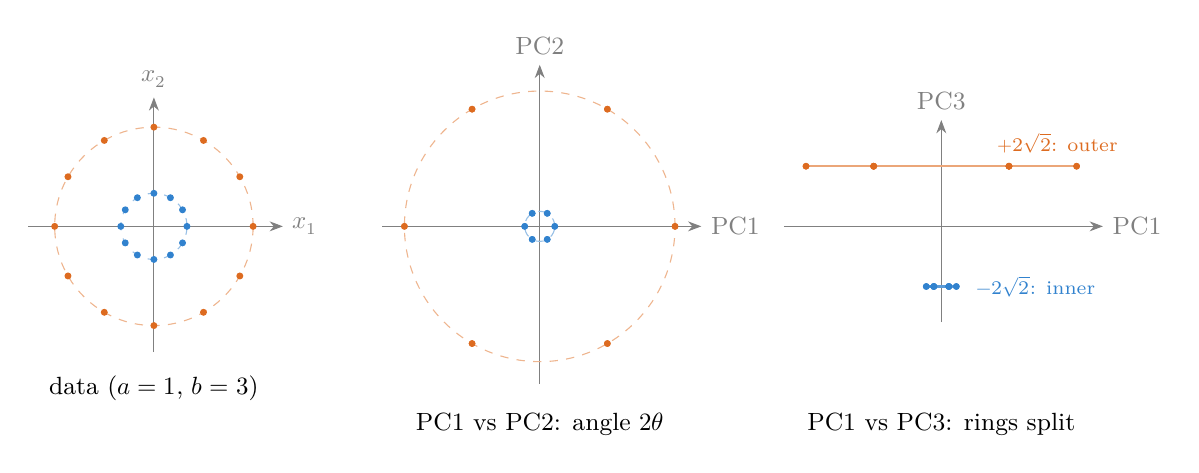
\begin{tikzpicture}
\begin{scope}[scale=0.42]
  \draw[-{Stealth}, gray] (-3.8,0) -- (3.9,0) node[right] {\small $x_1$};
  \draw[-{Stealth}, gray] (0,-3.8) -- (0,3.9) node[above] {\small $x_2$};
  \draw[dashed, dataC!50] (0,0) circle (1);
  \draw[dashed, accentC!50] (0,0) circle (3);
  \foreach \t in {0,30,...,330} { \fill[dataC] ({cos(\t)},{sin(\t)}) circle (3pt); \fill[accentC] ({3*cos(\t)},{3*sin(\t)}) circle (3pt); }
  \node[font=\small] at (0,-4.9) {data ($a=1$, $b=3$)};
\end{scope}
\begin{scope}[xshift=4.9cm, scale=0.27]
  \draw[-{Stealth}, gray] (-7.4,0) -- (7.6,0) node[right] {\small PC1};
  \draw[-{Stealth}, gray] (0,-7.4) -- (0,7.6) node[above] {\small PC2};
  \draw[dashed, accentC!50] (0,0) circle (6.364);
  \draw[dashed, dataC!50] (0,0) circle (0.707);
  \foreach \t in {0,30,...,330} { \fill[dataC] ({0.707*cos(2*\t)},{0.707*sin(2*\t)}) circle (4.5pt); \fill[accentC] ({6.364*cos(2*\t)},{6.364*sin(2*\t)}) circle (4.5pt); }
  \node[font=\small] at (0,-9.3) {PC1 vs PC2: angle $2\theta$};
\end{scope}
\begin{scope}[xshift=10cm, scale=0.27]
  \draw[-{Stealth}, gray] (-7.4,0) -- (7.6,0) node[right] {\small PC1};
  \draw[-{Stealth}, gray] (0,-4.5) -- (0,5) node[above] {\small PC3};
  \draw[accentC!60, thick] (-6.364,2.828) -- (6.364,2.828);
  \draw[dataC!80, thick] (-0.707,-2.828) -- (0.707,-2.828);
  \foreach \t in {0,30,...,330} { \fill[accentC] ({6.364*cos(2*\t)},2.828) circle (4.5pt); \fill[dataC] ({0.707*cos(2*\t)},-2.828) circle (4.5pt); }
  \node[font=\scriptsize, accentC, anchor=west] at (2.2,3.9) {$+2\sqrt2$: outer};
  \node[font=\scriptsize, dataC, anchor=west] at (1.2,-2.83) {$-2\sqrt2$: inner};
  \node[font=\small] at (0,-9.3) {PC1 vs PC3: rings split};
\end{scope}
\end{tikzpicture}
\caption{Kernel PCA with $k(\vx,\vy)=(1+\vx\T\vy)^2$ on two rings. In the PC1--PC2 plane each ring is a
circle traversed \emph{twice}, since the angle doubles. PC3 is constant on each ring, so it separates them.}
\end{figure}

\begin{intuition}
\textbf{Why the angle doubles.} Every feature in $\varphi$ is a polynomial of degree $\le2$, and the
quadratic ones satisfy $\varphi_q(-\vx)=\varphi_q(\vx)$. So the top PCs, built only from
quadratic features, cannot tell $\vx$ from $-\vx$. Opposite points on a ring land on the
same score, and going once around the ring goes twice around the score circle. The
linear features $\sqrt2x_1,\sqrt2x_2$ \emph{can} tell them apart, but they come later (PC4, PC5).
\end{intuition}

\begin{deeper}
\textbf{Kernel PCA inherits PCA's scale sensitivity.} The ordering above depends on the
size of the data. With $a=\tfrac12$, $b=1$: $m_2=0.625$, $\tfrac14m_4\approx0.133$, and
$\tfrac18(b^2-a^2)^2\approx0.070$. Now the \emph{linear} features are PC1 and PC2, and the ring
indicator falls to PC5. The ``$1+$'' in $(1+\vx\T\vy)^2$ fixes the relative weight of the linear
and quadratic features. Rescaling $\vx$ changes that balance, just as changing units changed
ordinary PCA (Section~2.6). One fact does not depend on scale: whenever $0<a<b$,
$(b^2-a^2)^2<a^4+b^4$, so the ring indicator always ranks below the two angle PCs.
\end{deeper}

\begin{deeper}
\textbf{The same rings with an RBF kernel.} Both the data distribution and the RBF kernel are
unchanged by rotations, so the kernel PCs split into ``angular frequencies'': functions of the form
$g(R)\cos m\theta$ or $g(R)\sin m\theta$. On two rings, a centered function of $R$ alone ($m=0$)
can only take one value per ring, so it \emph{is} the ring indicator. The kernel always
produces a ring indicator, but its rank depends on $\sigma$:
\begin{itemize}[nosep]
\item $\sigma$ \emph{smaller than the gap} $b-a$ (but larger than the spacing between neighbouring points):
the rings barely see each other, $K$ is nearly block-diagonal, and the strongest structure is
``which ring am I on''. The ring indicator tends to be PC1, like two clusters.
\item $\sigma$ \emph{much larger than} $b$: $e^{-\norm{\vx-\vy}^2/\sigma^2}\approx1-\norm{\vx-\vy}^2/\sigma^2$, and after
centering the kernel acts like the low-degree polynomial kernel. The linear angle modes
$\cos\theta,\sin\theta$ lead, and the ring indicator drops down the list.
\end{itemize}
This is the board's remark that the ring indicator ``will show up at different levels of importance''.
It is worth checking numerically: build $K$ for a few values of $\sigma$ and watch where the
two-valued eigenvector appears.
\end{deeper}

\subsection{Two views of the same scores}

\begin{center}
\begin{tabular}{p{0.44\linewidth}cp{0.44\linewidth}}
\textbf{Feature-space view.} Kernel PC scores are the coordinates of $\varphi(\vx_i)-\bar{\varphi}$
projected onto the directions of greatest variability of $\varphi(\vx_1),\dots,\varphi(\vx_N)$ in
$\mathcal F$. Linear, but in a big space.
& \raisebox{-1.2em}{\Large $=$} &
\textbf{$\R^d$ view.} Kernel PC scores are \emph{smooth nonlinear functions} of the coordinates of each
vector: $y_j(\vx)=\vw_j\T(\varphi(\vx)-\bar{\varphi})=\sum_i\alpha_{ij}\,k(\vx_i,\vx)+\text{const}$.
Nonlinear, but in the original space.
\end{tabular}
\end{center}
In the ring example the $\R^d$ view is explicit. PC1 is the function
$y_1(\vx)=\tfrac{x_1^2-x_2^2}{\sqrt2}$, PC3 is $y_3(\vx)=\tfrac{x_1^2+x_2^2-m_2}{\sqrt2}$, and so on.
The level sets of $y_3$ are circles, which is why it separates the rings. In general, the
kernel decides which family of functions the scores can come from: quadratics for the
degree-2 polynomial kernel, smooth bumps for the RBF kernel.

\subsection{Reconstruction, kernel tuning and anomaly detection}\label{sec:preimage}

In linear PCA, a point is rebuilt from its first $k$ scores as $\widehat{\vx}=\xbar+\sum_{j\le k}y_j\vw_j$ (Section~3.1). Kernel PCA
can do the same \emph{in feature space}, but the answer lives in $\mathcal F$, not in $\R^d$. Turning it back into a point
of $\R^d$ is called the \textbf{pre-image problem}, and it is what makes kernel PCA usable for tuning, anomaly
detection and denoising.

\begin{definition}{Feature-space reconstruction error}{rhodef}
Let $P_k$ be the orthogonal projection onto the span of the top $k$ kernel PCA loadings
$\vw_1,\dots,\vw_k\in\mathcal F$ (the board calls them $\bm\psi_1,\dots,\bm\psi_k$). For a point $\vx$ to be reconstructed and a candidate $\bm z\in\R^d$, define
\[
\rho_{\vx}(\bm z)=\big\|\,\varphi(\bm z)-\bar\varphi-P_k\big(\varphi(\vx)-\bar\varphi\big)\big\|^2 ,
\qquad
P_k(\bm v)=[\vw_1\cdots\vw_k]\begin{bmatrix}\vw_1\T\\\vdots\\\vw_k\T\end{bmatrix}\bm v=W_kW_k\T\bm v .
\]
$P_k(\varphi(\vx)-\bar\varphi)$ is the rank-$k$ approximation of $\varphi(\vx)$, its projection onto the best $k$-dimensional
hyperplane in feature space. $\rho_{\vx}(\bm z)$ measures how far $\varphi(\bm z)$ is from it. To keep formulas short, assume the
features are centered, $\bar\varphi=\tfrac1N\sum_i\varphi(\vx_i)=\bm0$; then $\rho_{\vx}(\bm z)=\norm{\varphi(\bm z)-P_k\varphi(\vx)}^2$.
\end{definition}

\begin{definition}{Pre-image (kernel PCA reconstruction)}{preimage}
\[
\widehat{\bm z}(\vx)=\argmin_{\bm z\in\R^d}\ \rho_{\vx}(\bm z)
\]
is the reconstruction of $\vx$ using the rank-$k$ approximation: the point of $\R^d$ whose feature vector is closest to
the projected feature vector of $\vx$. (``How well can I reconstruct my data?'')
\end{definition}

\begin{figure}[htbp]
\centering
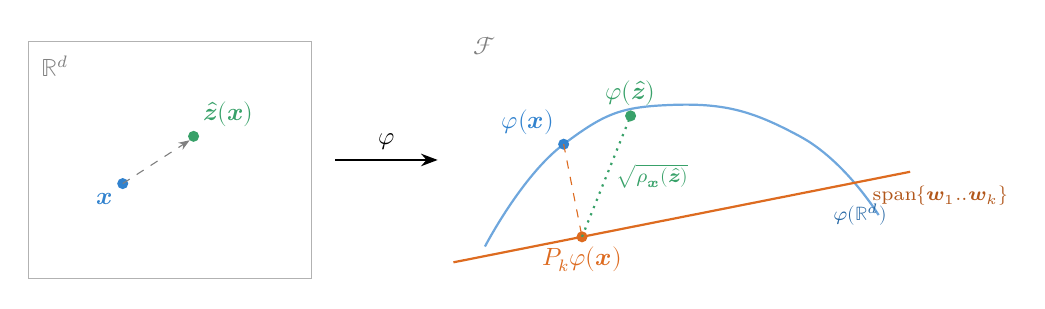
\begin{tikzpicture}[scale=1.0]
\begin{scope}
  \draw[gray!60] (-0.2,-0.2) rectangle (3.4,2.8);
  \node[gray, font=\small, anchor=north west] at (-0.15,2.75) {$\R^d$};
  \fill[dataC] (1.0,1.0) circle (2pt) node[below left, font=\small] {$\vx$};
  \fill[accentD] (1.9,1.6) circle (2pt) node[above right, font=\small] {$\widehat{\bm z}(\vx)$};
  \draw[dashed, gray, -{Stealth[length=4pt]}] (1.0,1.0) -- (1.85,1.55);
\end{scope}
\draw[-{Stealth[length=6pt]}, thick] (3.7,1.3) -- node[above, font=\small] {$\varphi$} (5.0,1.3);
\begin{scope}[xshift=5.4cm]
  \node[gray, font=\small] at (0.2,2.75) {$\mathcal F$};
  % image of phi: curved manifold
  \draw[thick, dataC!70] plot[smooth, tension=0.8] coordinates {(0.2,0.2) (1.2,1.5) (2.6,2.0) (4.2,1.6) (5.2,0.6)};
  \node[dataC!80!black, font=\scriptsize, anchor=west] at (4.5,0.6) {$\varphi(\R^d)$};
  % k-dim subspace (line)
  \draw[thick, accentC] (-0.2,0.0) -- (5.6,1.15);
  \node[accentC!80!black, font=\scriptsize, anchor=west] at (5.0,0.85) {span$\{\vw_1..\vw_k\}$};
  % phi(x) on curve, its projection on line
  \coordinate (Fx) at (1.2,1.5);
  \fill[dataC] (Fx) circle (2pt) node[above left, font=\small] {$\varphi(\vx)$};
  \coordinate (Px) at ($(-0.2,0.0)!(Fx)!(5.6,1.15)$);
  \draw[dashed, accentC] (Fx) -- (Px);
  \fill[accentC] (Px) circle (2pt) node[below, font=\small] {$P_k\varphi(\vx)$};
  % nearest point on curve to Px
  \coordinate (Fz) at (2.05,1.86);
  \fill[accentD] (Fz) circle (2pt) node[above, font=\small] {$\varphi(\widehat{\bm z})$};
  \draw[accentD, thick, dotted] (Px) -- (Fz) node[midway, right, font=\scriptsize] {$\sqrt{\rho_{\vx}(\widehat{\bm z})}$};
\end{scope}
\end{tikzpicture}
\caption{The pre-image problem. Feature vectors of real points lie on the curved set $\varphi(\R^d)$. The rank-$k$
approximation $P_k\varphi(\vx)$ lies on the flat span of the loadings and is usually \emph{not} the image of any point.
So we look for the point $\widehat{\bm z}$ whose image $\varphi(\widehat{\bm z})$ comes closest to it.}
\end{figure}

\subsubsection*{Computing $\rho$ with kernels only}

The loadings are never formed, so $\rho$ has to be rewritten in kernel evaluations. Two observations do it.

\textbf{(1) The loadings live in the span of the data.} Write the centered feature matrix as $\widetilde X$ (rows $\varphi(\vx_i)\T$) with SVD
$\widetilde X=US\widetilde V\T$. Then (assuming $\bar\varphi=\bm0$)
\[
K=HKH=\widetilde X\widetilde X\T=US\,S\,U\T=UD^{1/2}D^{1/2}U\T,\qquad D=S^2=\diag(\mu_1,\mu_2,\dots),
\]
so the scores are $\widetilde X\widetilde V=US=UD^{1/2}$, and the loadings $\widetilde V$ (in feature space) are recovered from $U$: multiply
$\widetilde X=US\widetilde V\T$ on the left by $S^{-1}U\T$ to get
\[
\widetilde V\T=S^{-1}U\T\widetilde X=\begin{bmatrix}\vw_1\T\\\vdots\\\vw_r\T\end{bmatrix},\qquad \vw_j=\frac{1}{\sqrt{\mu_j}}\sum_{i=1}^Nu_{ij}\,\varphi(\vx_i).
\]
Each loading is a combination of data features: $\spn(\text{loadings})\subseteq\spn(\text{data})$ (Theorem~\ref{thm:kscores}(iii)).

\textbf{(2) Expand the squared distance.} $P_k=W_kW_k\T$ is a projection ($W_k\T W_k=I$), so
\[
\rho_{\vx}(\bm z)=\varphi(\bm z)\T\varphi(\bm z)-2\,\varphi(\bm z)\T W_kW_k\T\varphi(\vx)+\norm{W_k\T\varphi(\vx)}^2 .
\]
With $\bm\kappa(\bm a)=\big(k(\vx_1,\bm a),\dots,k(\vx_N,\bm a)\big)\T$ (kernel values against the training points),
\[
W_k\T\varphi(\bm a)=S_k^{-1}U_k\T\widetilde X\varphi(\bm a)=D_k^{-1/2}U_k\T\bm\kappa(\bm a),
\]
so
\[
\boxed{\ \rho_{\vx}(\bm z)=k(\bm z,\bm z)-2\,\bm\kappa(\bm z)\T\,U_kD_k^{-1}U_k\T\,\bm\kappa(\vx)+\bm\kappa(\vx)\T\,U_kD_k^{-1}U_k\T\,\bm\kappa(\vx)\ }
\]
Only kernel evaluations appear: $k(\bm z,\bm z)$, $k(\bm z,\vx_i)$ and $k(\vx,\vx_i)$. (Without the assumption $\bar\varphi=\bm0$, replace $k$ by the
centered kernel $\tilde k(\bm a,\bm b)=k(\bm a,\bm b)-\tfrac1N\sum_lk(\bm a,\vx_l)-\tfrac1N\sum_lk(\vx_l,\bm b)+\tfrac1{N^2}\sum_{l,m}K_{lm}$, as in Prop.~\ref{prop:centerk}.)
The last term does not depend on $\bm z$, so minimizing over $\bm z$ only needs the first two.

\begin{intuition}
\textbf{Sanity check with the linear kernel.} If $k(\bm a,\bm b)=\bm a\T\bm b$, then $\varphi$ is the identity, $\varphi(\R^d)$ is all of $\R^d$, and
$\rho_{\vx}(\bm z)=\norm{\bm z-\xbar-P_k(\vx-\xbar)}^2$. The minimizer is $\widehat{\bm z}=\xbar+P_k(\vx-\xbar)$, exactly the ordinary PCA
reconstruction, with $\rho=0$. With a nonlinear kernel $\varphi(\R^d)$ is curved, the projected point usually falls off it,
and the minimum is positive. The reconstructions then land on a \emph{nonlinear} surface learned from the data,
the way linear PCA reconstructions land on a flat one.
\end{intuition}

\begin{careful}
\textbf{No closed form.} $\rho_{\vx}(\bm z)$ is a nonlinear, generally non-convex function of $\bm z$, so $\widehat{\bm z}$ is found
numerically (gradient descent, several starting points, e.g.\ starting at $\vx$). For the RBF kernel $k(\bm z,\bm z)=1$ is constant,
so minimizing $\rho$ means maximizing $\bm\kappa(\bm z)\T\bm\gamma$ with $\bm\gamma=U_kD_k^{-1}U_k\T\bm\kappa(\vx)$. Setting the gradient to zero gives the
fixed-point iteration
$\bm z\leftarrow\sum_i\gamma_ik(\bm z,\vx_i)\vx_i\big/\sum_i\gamma_ik(\bm z,\vx_i)$, a weighted average of training points (Mika et al., 1999).
\end{careful}

\subsubsection*{Three uses of the pre-image}

\textbf{1) Cross-validation for kernel tuning and selection.} Kernel PCA results depend heavily on the kernel
and its parameters (Section~7.6), and on the training data alone more flexibility always looks better. So:
\begin{enumerate}[nosep,label=(\roman*)]
\item split the data into two sets, train and test;
\item learn the kernel PCA (scores, $U_k$, $D_k$) from the train set only, then compute the test error
\[
\text{CV}(k,\text{kernel},\text{params})=\sum_{\vx\in\text{test}}\ \min_{\bm z}\ \rho_{\vx}(\bm z);
\]
\item minimize over the choice of parameters and kernels (and $k$).
\end{enumerate}

\begin{careful}
\textbf{Why a held-out set, and a caution.} On the training points, using all $N-1$ components reproduces every
$\varphi(\vx_i)$ exactly (they lie in the span of the data), so training error can be driven to $0$ by any kernel. Test points
reveal whether the learned surface generalizes. Also, $\rho$ is measured in each kernel's \emph{own} feature space,
whose scale differs between kernels (e.g.\ $k(\bm z,\bm z)=1$ for RBF but unbounded for polynomials). Comparing parameters
within one kernel family is fine. Comparing \emph{different} kernels is safer with an input-space error such as
$\sum_{\vx\in\text{test}}\norm{\vx-\widehat{\bm z}(\vx)}^2$.
\end{careful}

\textbf{2) Anomaly detection.} Reconstruct each point and measure how far the reconstruction moved it:
\[
\text{score}(\vx_i)=\norm{\widehat{\bm z}(\vx_i)-\vx_i}=\Big\|\argmin_{\bm z}\rho_{\vx_i}(\bm z)-\vx_i\Big\| .
\]
A \textbf{large} value flags an anomaly: the point is poorly explained by the nonlinear structure that the other
points share. (The feature-space error $\min_{\bm z}\rho_{\vx_i}(\bm z)$, or the simpler $\norm{(I-P_k)\varphi(\vx_i)}^2$, works as a score too.)

\textbf{3) Denoising and generation (augmentation).} Pick \emph{any} point $\tilde{\vx}$, e.g.\ a noisy sample or a perturbed
data point, not necessarily in the data set, and compute $\argmin_{\bm z}\rho_{\tilde{\vx}}(\bm z)$. The result is a point of $\R^d$ that matches
the nonlinear structure of your data: you pick points in Euclidean space and pull them onto the learned surface.
Applied to noisy inputs this \emph{denoises} (the classic example is denoised handwritten digits); applied to random
perturbations of data points it \emph{generates} new, realistic-looking samples.

\begin{deeper}
All three uses are the same idea as linear PCA's ``reconstruct and look at the residual'', with the flat
hyperplane replaced by a curved surface. Large residual: anomaly. Small residual on held-out data: good kernel.
Project an arbitrary point: denoised or generated sample.
\end{deeper}

\subsection{The spectral view: eigenfunctions, Mercer's theorem, and what $\widetilde K$ estimates}\label{sec:spectral}

So far everything was about a finite sample. Now suppose the data are i.i.d.\ draws from a
density $f$ on $\R^d$, and ask what kernel PCA converges to as $N\to\infty$.

\textbf{The population centered kernel.} The continuous analogue of $\widetilde K=HKH$ replaces each
row/column average by an integral against $f$:
\[
\tilde k(\vx,\vy)=k(\vx,\vy)-\int k(\vx,\vy')f(\vy')\,d\vy'-\int k(\vx',\vy)f(\vx')\,d\vx'+\iint k(\vx',\vy')f(\vx')f(\vy')\,d\vx'\,d\vy' .
\]
Term by term this matches Prop.~\ref{prop:centerk}: subtract the row average, subtract the column
average, add back the grand average. Expanding the inner product shows
$\tilde k(\vx,\vy)=\langle\varphi(\vx)-\mathbb E\varphi,\ \varphi(\vy)-\mathbb E\varphi\rangle$, so $\tilde k$ is the kernel of the
\emph{centered} feature map. Hence \textbf{if $k$ satisfies Mercer's condition, so does $\tilde k$}:
every kernel matrix of $\tilde k$ is a Gram matrix of the centered features, which is PSD by
Theorem~\ref{thm:mercerfeat}(a).

\textbf{From matrices to operators.} A matrix acts on a vector by
summing over an index. The analogous object here acts on a \emph{function} by integrating
against the data density:
\[
(T_fg)(\vx)=\int\tilde k(\vx,\vy)\,g(\vy)\,f(\vy)\,d\vy
\qquad\longleftrightarrow\qquad
(K\bm g)_i=\sum_jK_{ij}g_j .
\]
\begin{center}
\renewcommand{\arraystretch}{1.25}
\begin{tabular}{lll}
\toprule
& finite (matrix) & population (operator) \\
\midrule
object & $\widetilde K\in\R^{N\times N}$ & $T_f$ acting on functions $g:\R^d\to\R$ \\
eigen-equation & $\widetilde K\vu=\mu\vu$ & $T_f\psi=\mu\,\psi$ \\
orthonormality & $\vu_\ell\T\vu_m=\delta_{\ell m}$ & $\int\psi_\ell(\vx)\psi_m(\vx)f(\vx)\,d\vx=\delta_{\ell m}$ \\
decomposition & $\widetilde K_{ij}=\sum_\ell\mu_\ell u_{i\ell}u_{j\ell}$ & $\tilde k(\vx,\vy)=\sum_\ell\mu_\ell\psi_\ell(\vx)\psi_\ell(\vy)$ \\
\bottomrule
\end{tabular}
\end{center}

\begin{definition}{Eigenfunctions}{eigfun}
A function $\psi_\ell$ is an \textbf{eigenfunction} of $T_f$ with eigenvalue $\mu_\ell$ if
$(T_f\psi_\ell)(\vx)=\mu_\ell\psi_\ell(\vx)$ for all $\vx$, i.e.\ $\int\tilde k(\vx,\vy)\psi_\ell(\vy)f(\vy)\,d\vy=\mu_\ell\psi_\ell(\vx)$.
Applying $T_f$ only rescales $\psi_\ell$, just as a matrix only rescales an eigenvector. We normalize so that
$\int\psi_\ell\psi_mf\,d\vx=1$ if $m=\ell$ and $0$ otherwise. This is ``orthonormal'' with
inner product $\langle g,h\rangle_f=\int ghf$, which weights each region by how much data lives there.
\end{definition}

\begin{theorem}{Mercer's theorem}{mercerthm}
Suppose $\tilde k$ is a continuous, symmetric kernel satisfying Mercer's condition, and the
integral operator is well behaved (for instance $\int\!\!\int\tilde k(\vx,\vy)^2f(\vx)f(\vy)\,d\vx\,d\vy<\infty$). Then $T_f$
has eigenfunctions $\psi_1,\psi_2,\dots$ with eigenvalues $\mu_1\ge\mu_2\ge\cdots\ge0$, and
\[
\tilde k(\vx,\vy)=\sum_{\ell=1}^{\infty}\mu_\ell\,\psi_\ell(\vx)\,\psi_\ell(\vy).
\]
\end{theorem}

\begin{intuition}
This is the spectral theorem $A=\sum_\ell\lambda_\ell\vq_\ell\vq_\ell\T$ with the index $i$ replaced by a
point $\vx$. It also hands us an explicit feature map. Set
\[
\Phi(\vx)=\big(\sqrt{\mu_1}\,\psi_1(\vx),\ \sqrt{\mu_2}\,\psi_2(\vx),\ \dots\big).
\]
Then $\langle\Phi(\vx),\Phi(\vy)\rangle=\sum_\ell\mu_\ell\psi_\ell(\vx)\psi_\ell(\vy)=\tilde k(\vx,\vy)$, which is the converse
half of Theorem~\ref{thm:mercerfeat}. These coordinates are already the \textbf{population kernel PCs}:
coordinate $\ell$ has variance $\mu_\ell\int\psi_\ell^2f=\mu_\ell$, and different coordinates are
uncorrelated because $\int\psi_\ell\psi_mf=0$. (They also have mean zero: centering gives
$\int\tilde k(\vx,\vy)f(\vy)\,d\vy=0$, so the constant function is in the null space, and every $\psi_\ell$
with $\mu_\ell>0$ is orthogonal to it.)
\end{intuition}

\subsubsection*{Kernel PCA approximates the spectral decomposition}

Replace integrals by averages over the sample. If $\vx_1,\dots,\vx_N\overset{\text{iid}}{\sim}f$ and
$\bm g=(g(\vx_1),\dots,g(\vx_N))\T$, then
\[
(T_fg)(\vx_i)=\int\tilde k(\vx_i,\vy)g(\vy)f(\vy)\,d\vy\ \approx\ \frac1N\sum_{j=1}^N\tilde k(\vx_i,\vx_j)\,g(\vx_j)
=\Big(\tfrac1N\widetilde K\bm g\Big)_i .
\]
(This uses the sample-centered $\widetilde K$ in place of $\tilde k$; the two agree as $N\to\infty$.) So the
eigen-equation $T_f\psi=\mu\psi$, evaluated at the data points, becomes
$\tfrac1N\widetilde K\bm\psi\approx\mu\bm\psi$. Therefore:
\begin{itemize}[nosep]
\item the eigenvalues of $\tfrac1N\widetilde K$, which are the kernel PC variances $\mu_j/N$ of the algorithm, estimate the operator eigenvalues;
\item the eigenvectors of $\widetilde K$ are the eigenfunctions \emph{sampled at the data}. Matching the normalizations
$\tfrac1N\sum_i\psi_\ell(\vx_i)^2\approx\int\psi_\ell^2f=1$ and $\norm{\vu_\ell}=1$ gives
\[
\psi_\ell(\vx_i)\approx\sqrt N\,u_{i\ell}\qquad(\text{up to sign}).
\]
\end{itemize}
Plugging in, the kernel PC score of $\vx_i$ is
$\sqrt{\text{eigenvalue of }\widetilde K}\cdot u_{i\ell}\approx\sqrt{N\mu_\ell}\cdot\tfrac{\psi_\ell(\vx_i)}{\sqrt N}=\sqrt{\mu_\ell}\,\psi_\ell(\vx_i)$,
which is exactly the Mercer coordinate $\Phi_\ell(\vx_i)$.

\begin{intuition}
\textbf{Kernel PCA is the finite-sample estimate of the Mercer expansion.} The eigen-decomposition
in Algorithm~\ref{alg:kpca} is not just a computational trick. It estimates the natural ``modes''
of the data distribution as seen through the kernel. In the ring example the top eigenfunctions
are proportional to $R^2\cos2\theta$, $R^2\sin2\theta$ and $R^2-m_2$, which are the score functions in the table.
\end{intuition}

\begin{careful}
Three details that short explanations often skip. (1) The match ``eigenvector entry $\leftrightarrow$
eigenfunction value'' holds only up to the factor $\sqrt N$ and a sign. (2) The eigenfunctions
belong to the \emph{centered} kernel and depend on the data density $f$, not on $k$ alone. The same kernel on a
different distribution has different eigenfunctions. (3) Distinguish three objects: the kernel
function $k(\vx,\vy)$; the finite matrix $K$ built from your sample; and the operator $T_f$ that
Mercer's theorem is about.
\end{careful}

\begin{deeper}
A clean example: points uniform on a circle with the RBF kernel. Then $k$ depends only on the angle
difference $\theta-\theta'$, so $T_f$ is a convolution on the circle, and convolutions are diagonalized by
Fourier modes. The eigenfunctions are the constant, then $\cos\theta,\sin\theta$, then
$\cos2\theta,\sin2\theta$, and so on, ordered from smooth to wiggly. Centering removes the constant. The
top kernel PCs are therefore smooth waves around the circle.
\end{deeper}

% ==================================================================
\section{Manifold Learning}\label{sec:manifold}
% ==================================================================

Kernel PCA tried to straighten curved data by lifting it into a feature space. Manifold learning attacks the curve
\emph{directly}: assume the data lie on a curved, low-dimensional surface inside $\R^d$, and try to recover coordinates
\emph{on} that surface.

\subsection{The manifold hypothesis}

\begin{definition}{Manifold hypothesis}{manhyp}
High-dimensional data sets tend to concentrate near a \textbf{sub-manifold} whose \textbf{intrinsic dimension} is much lower
than the dimension $d$ of the \textbf{ambient space} $\R^d$.
\end{definition}

\begin{intuition}
A $256\times256$ photo of a face is a point in $\R^{65{,}536}$, but the photos you would actually call ``faces'' vary along a handful
of directions (pose, lighting, expression, identity), so they occupy a thin, curved sliver of that huge space. The
lecture's analogy is the brain: it compresses high-dimensional sensory input into a simpler internal representation, a
kind of world model, and that simpler representation is what lets it learn and generalize to new situations. Working
in the intrinsic coordinates is the statistical version of the same idea. The vocabulary of ambient, intrinsic and linear
dimension is Definition~\ref{def:dims}. PCA measures only the linear one, and manifold learning targets the intrinsic one.
\end{intuition}

\subsection{What is a manifold?}

\begin{definition}{(Topological) manifold}{manifold}
A space $M$ is a $t$-dimensional \textbf{manifold} if every point $\bm p\in M$ has an open neighborhood $U_{\bm p}\subseteq M$ that can be
continuously transformed, with a continuous inverse, onto an open subset of $\R^t$. In short, $M$ \textbf{locally resembles
Euclidean space}. A \textbf{sub-manifold} of $\R^d$ is a manifold sitting inside $\R^d$ (with $t\le d$).
\end{definition}

\begin{intuition}
Zoom in far enough at any point and the space looks flat: a short piece of a circle looks like a line, and a small
patch of the Earth looks like a flat map, even though the whole thing is round. ``Topological'' means we only need
nearness (open neighborhoods), not yet distances or derivatives.
\end{intuition}

\begin{example}{Manifolds and non-manifolds}{manex}
\begin{itemize}[nosep]
\item \textbf{$1$-dimensional:} an open line segment and a circle. Each locally looks like $\R^1$.
\item \textbf{$2$-dimensional:} a sphere (the Earth's surface). Zoomed in, it is a $2$D plane.
\item \textbf{Flat ones:} for independent $\bm v_1,\dots,\bm v_k\in\R^d$ ($k<d$), the subspace $\spn\{\bm v_1,\dots,\bm v_k\}$ is a sub-manifold of
$\R^d$ of intrinsic dimension $k$. Every PCA subspace is a (flat) manifold, so manifolds generalize what PCA fits.
\item \textbf{Not a manifold: the figure-8.} At the crossing point, every small neighborhood looks like an ``X'' with four
branches. Remove the crossing point and it falls into four pieces, while removing a point from a small interval of $\R^1$
leaves two pieces, so it is not like $\R^1$. It is too thin to be like $\R^2$. No dimension works there.
\item \textbf{Edges:} a segment \emph{with} its endpoints, or a rectangle with its border, fails at the edge points, where
the neighborhood is only a half-line or half-plane. These are \emph{manifolds with boundary}. Using open sets (as in
the Swiss roll's rectangle below) avoids the issue.
\end{itemize}
\end{example}

\begin{definition}{Charts and atlases}{charts}
A \textbf{chart} is a map $\phi_{\bm p}:U_{\bm p}\to\R^t$ that flattens a piece of $M$ onto Euclidean coordinates. Calculus is easy in
$\R^t$, so you work in the chart and map back with $\phi_{\bm p}^{-1}$. A collection of charts covering all of $M$ is an
\textbf{atlas} (exactly like a world atlas: each page is a flat map of part of the globe, and the pages overlap). If the
change of coordinates between overlapping charts is differentiable, $M$ is a \textbf{differentiable manifold}, and tangent
spaces (below) make sense.
\end{definition}

\subsection{A concrete example: the Swiss roll}

\begin{example}{Swiss roll}{swissroll}
Take the open rectangle $A=\big(\tfrac{3\pi}2,\tfrac{9\pi}2\big)\times(0,15)\subseteq\R^2$ and the map
\[
\psi:A\to\R^3,\qquad \psi(y_1,y_2)=\begin{bmatrix}y_1\cos y_1\\ y_1\sin y_1\\ y_2\end{bmatrix}.
\]
The first two coordinates trace a spiral whose radius $y_1$ grows as it turns, and $y_2$ stretches it out sideways. The
image $M=\psi(A)$ is the Swiss roll: \textbf{ambient dimension $3$, intrinsic dimension $2$}.

\textbf{Generating data on the manifold:} sample $\bm y_1,\dots,\bm y_N\sim\mathrm{Unif}(A)$ and set $\vx_i=\psi(\bm y_i)$.
\end{example}

\begin{figure}[htbp]
\centering
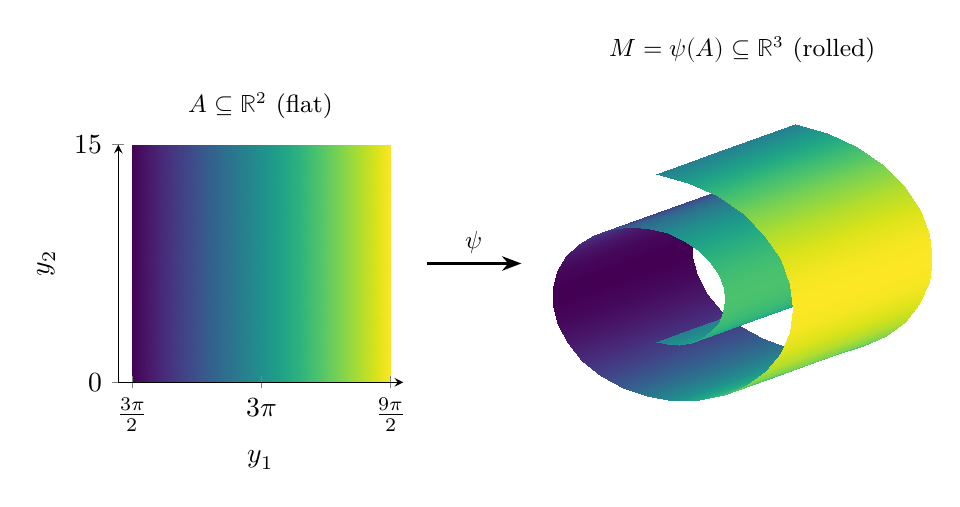
\begin{tikzpicture}
\begin{axis}[name=rect, width=5.2cm, height=4.6cm, axis lines=left, xlabel={$y_1$}, ylabel={$y_2$},
  xmin=4.2, xmax=14.6, ymin=0, ymax=15, xtick={4.712,9.425,14.137}, xticklabels={$\frac{3\pi}2$,$3\pi$,$\frac{9\pi}2$},
  ytick={0,15}, colormap/viridis, view={0}{90}, title={\small $A\subseteq\R^2$ (flat)}]
\addplot3[surf, shader=interp, domain=4.712:14.137, y domain=0:15, samples=30, samples y=2, point meta=x] (x,y,0);
\end{axis}
\draw[-{Stealth[length=7pt]}, thick] ($(rect.east)+(0.3,0)$) -- node[above, font=\small] {$\psi$} ($(rect.east)+(1.5,0)$);
\begin{axis}[at={(rect.east)}, anchor=west, xshift=1.9cm, view={30}{12}, width=6.4cm, height=6cm, axis lines=none,
  colormap/viridis, title={\small $M=\psi(A)\subseteq\R^3$ (rolled)}]
\addplot3[surf, shader=interp, z buffer=sort, domain=4.712:14.137, y domain=0:15, samples=45, samples y=6, point meta=x]
  ({x*cos(deg(x))},{y},{x*sin(deg(x))});
\end{axis}
\end{tikzpicture}
\caption{The Swiss roll. Colour shows $y_1$, the coordinate along the spiral. Manifold learning is the reverse
direction: given only points on the roll (right), recover the flat coordinates (left).}
\end{figure}

\begin{careful}
\textbf{Uniform on $A$ is not uniform on $M$.} $\psi$ stretches the $y_1$ direction by $\norm{\partial\psi/\partial y_1}=\sqrt{1+y_1^2}$ (computed
below), so outer turns of the roll ($y_1$ large) are stretched more and their points are spread more thinly. Sampling
$\mathrm{Unif}(A)$ puts \emph{fewer points per unit area} on the outer layers. Algorithms that rely on local density
notice this.
\end{careful}

\subsection{The manifold learning problem}

\begin{definition}{Goal of manifold learning}{mlgoal}
\textbf{In practice} we are given only $\vx_1,\dots,\vx_N\in\R^d$, plus the \emph{assumption} that they lie on, or near (if corrupted
by noise), a manifold $M$. We cannot check this assumption directly. The goal is to recover low-dimensional coordinates
$\bm y_1,\dots,\bm y_N\in\R^t$ and, if possible, the map $\psi$ or its inverse $\psi^{-1}:M\to A$.
\end{definition}

\textbf{Problems.}
\begin{enumerate}[label=\arabic*)]
\item \textbf{The intrinsic dimension $t$ is unknown}, and has to be estimated from the data too.
\item \textbf{There is no unique solution.} Suppose we found $\bm y_1,\dots,\bm y_N$ and $\psi$ with $\psi(\bm y_i)=\vx_i$. Take \emph{any} invertible
$g:\R^t\to\R^t$ and set $\bm z_i=g(\bm y_i)$. Then
\[
(\psi\circ g^{-1})(\bm z_i)=\psi(\bm y_i)=\vx_i ,
\]
so $\{\bm z_i\}$ with the map $\psi\circ g^{-1}$ explains the data equally well. The coordinates can be stretched, bent or folded at will.
\end{enumerate}

\begin{intuition}
\textbf{Fixing the non-uniqueness: constrain $\psi$.} The standard choice is to ask for an \textbf{isometric} embedding, one that
preserves distances \emph{measured along the manifold} (geodesic distances). Then $g$ can only be a rigid motion (rotation,
reflection, translation), the same leftover ambiguity as MDS (Section~6.2). Distance-preserving maps were also the
goal of metric MDS and the Sammon mapping (Section~6.6), which is why those reappear here. In practice the recovered
coordinates are \emph{qualitatively} right, up to rotation, translation and scaling. Note that the Swiss roll's own $\psi$ is
\emph{not} an isometry (it stretches $y_1$ by $\sqrt{1+y_1^2}$), so even a perfect algorithm returns an unrolled sheet that is
distorted relative to $A$.
\end{intuition}

\begin{careful}
\textbf{Why not just PCA or kernel PCA?} PCA projects onto a flat plane, so it squashes the layers of the roll on
top of each other: points far apart \emph{along} the roll but close in $\R^3$ (adjacent layers) land together. Kernel PCA can
bend, but its result depends heavily on the kernel and its tuning (Section~7.6), and it does not target the
manifold's own coordinates. Manifold learning instead works \emph{locally}, where the manifold is nearly flat.
\end{careful}

\subsection{Tangent spaces and tangent planes}

The local, flat approximation to a manifold at a point is its tangent space: the linear-algebra object that makes
``locally Euclidean'' concrete.

\begin{example}{Tangent line of a helix}{helixtangent}
$\psi:(0,6\pi)\to\R^3$, $\ \psi(s)=\big(\tfrac1{\sqrt2}\cos s,\ \tfrac1{\sqrt2}\sin s,\ \tfrac1{\sqrt2}s\big)$. Its velocity is
\[
\frac{d\psi}{ds}=\Big(-\tfrac1{\sqrt2}\sin s,\ \tfrac1{\sqrt2}\cos s,\ \tfrac1{\sqrt2}\Big),\qquad \Big\|\frac{d\psi}{ds}\Big\|^2=\tfrac12(\sin^2s+\cos^2s)+\tfrac12=1 ,
\]
so the $\tfrac1{\sqrt2}$'s make this a \emph{unit-speed} (arc-length) parametrization. At a point $\bm p=\psi(s)$, the \textbf{tangent space} is
\[
T_M(\bm p)=\spn\Big\{\frac{d\psi}{ds}\Big|_{s:\ \psi(s)=\bm p}\Big\},
\]
a line through the origin. The \textbf{tangent line} is $\bm p+T_M(\bm p)$, the same line moved to pass through $\bm p$.
\end{example}

\begin{definition}{Tangent space via the Jacobian}{tangent}
For a parametrization $\psi:A\subseteq\R^t\to\R^d$, the \textbf{Jacobian} collects the partial derivatives as columns,
\[
J_\psi=\Big[\frac{\partial\psi}{\partial y_1}\ \cdots\ \frac{\partial\psi}{\partial y_t}\Big]\in\R^{d\times t}.
\]
Evaluated at the parameter $\bm y$ with $\psi(\bm y)=\bm p$, its \textbf{columns span the tangent space}: $T_M(\bm p)=\col J_\psi(\bm y)$, a $t$-dimensional
\emph{linear} subspace when $J_\psi$ has full column rank $t$. The \textbf{tangent plane} is the \emph{affine} subspace $\bm p+T_M(\bm p)$.
\end{definition}

\begin{example}{Tangent plane of the Swiss roll}{srtangent}
With $\psi(s,t)=(s\cos s,\ s\sin s,\ t)$,
\[
J_\psi=\Big[\frac{\partial\psi}{\partial s}\ \ \frac{\partial\psi}{\partial t}\Big]=\begin{bmatrix}\cos s-s\sin s&0\\ \sin s+s\cos s&0\\ 0&1\end{bmatrix}\in\R^{3\times2},
\qquad
T_M(\bm p)=\spn\left\{\begin{bmatrix}\cos s-s\sin s\\\sin s+s\cos s\\0\end{bmatrix},\begin{bmatrix}0\\0\\1\end{bmatrix}\right\}
\]
evaluated at the $(s,t)$ with $\psi(s,t)=\bm p$. (Product rule: $\tfrac{d}{ds}(s\cos s)=\cos s-s\sin s$.) The two columns are orthogonal, and the first
has length $\sqrt{(\cos s-s\sin s)^2+(\sin s+s\cos s)^2}=\sqrt{1+s^2}>0$, so the rank is $2$ everywhere: a genuine plane at every point.
\end{example}

\begin{intuition}
\textbf{Why tangent planes matter: they localize the data.} Near $\bm p$ the manifold is almost its tangent plane. Project
the nearby data points onto $\bm p+T_M(\bm p)$ and read off their coordinates in a basis of $T_M(\bm p)$: those $t$ numbers are good
\emph{local} coordinates for the neighborhood. Manifold learning then has to glue the local coordinates from many
neighborhoods into one global set, just as an atlas glues overlapping map pages into a picture of the world.
\end{intuition}

\begin{deeper}
\textbf{The open question} was how to approximate the tangent plane at a point from the data alone, without $\psi$. The
answer, local SVD or local PCA, is the next section. PCA's weakness, that it only fits flat things, becomes a strength
once you only ask it to fit a small, nearly flat piece.
\end{deeper}

\subsection{Estimating tangent spaces from data: local SVD and local PCA}\label{sec:localpca}

In practice we have \textbf{no access to $\psi$ or to the latent $\bm y_1,\dots,\bm y_N$}, only $\vx_1,\dots,\vx_N$. So the Jacobian is out of
reach, and we want to approximate, at each data point $\vx_i$:
\begin{enumerate}[nosep,label=\arabic*)]
\item the tangent space $T_M(\vx_i)$;
\item the approximating hyperplane to $M$ at $\vx_i$;
\item local coordinates for the points in a neighborhood of $\vx_i$;
\item and, along the way, the intrinsic dimension $t$ of $M$.
\end{enumerate}

\begin{definition}{Local coordinates}{localcoords}
The \textbf{local coordinates} of points in a neighborhood of $\vx_i\in M$ are the coordinates obtained after continuously
mapping that neighborhood to $\R^t$: a chart (Definition~\ref{def:charts}), flattening the curved patch around $\vx_i$ into a
flat piece of $\R^t$.
\end{definition}

\begin{algorithm}{Local SVD at $\vx_i$}{localsvd}
\begin{enumerate}[nosep,label=\arabic*)]
\item \textbf{Neighbors.} Find the $k$ points closest to $\vx_i$ in Euclidean distance, $\vx_{(1)},\dots,\vx_{(k)}$. (Assumption: inside this
small ball, Euclidean distance is a good stand-in for distance along $M$; outside it, it may not be.)
\item \textbf{Center at $\vx_i$} (``define $\vx_i$ to be the origin''): form the rows $(\vx_{(1)}-\vx_i)\T,\dots,(\vx_{(k)}-\vx_i)\T$.
\item \textbf{SVD} of that $k\times d$ matrix, $X_c=\widehat U\widehat S\widehat V\T$, a low-rank approximation of the neighborhood.
\item \textbf{Read off the answers.}
\begin{itemize}[nosep]
\item \emph{Intrinsic dimension:} a scree plot of the singular values. Look for the gap: the first $t$ are large, the rest small.
\item \emph{Tangent space:} $T_M(\vx_i)\approx\spn\{\vv_1,\dots,\vv_t\}$, the first $t$ right singular vectors.
\item \emph{Approximating hyperplane:} $\vx_i+\spn\{\vv_1,\dots,\vv_t\}$.
\item \emph{Local coordinates:} the first $t$ columns of $\widehat U\widehat S$, i.e.\ row $j$ gives neighbor $j$'s coordinates in the tangent plane.
\end{itemize}
\end{enumerate}
\end{algorithm}

\begin{algorithm}{Local PCA at $\vx_i$}{localpcaalg}
Same neighbors, but \textbf{center at their mean} $\bar{\vx}_{(i)}=\tfrac1k\sum_j\vx_{(j)}$ instead of at $\vx_i$, then run ordinary PCA. Scree plot of the
eigenvalues for $t$; the first $t$ \emph{loadings} span the tangent space; the hyperplane is $\bar{\vx}_{(i)}+\spn\{\text{loadings}\}$; the first $t$ \emph{PC scores}
are the local coordinates.
\end{algorithm}

\begin{intuition}
\textbf{Why this works.} Zoom in on a manifold and it looks flat (Section~\ref{sec:manifold}). A small neighborhood of a
$t$-dimensional manifold is nearly a $t$-dimensional flat piece, so a rank-$t$ approximation of the neighborhood captures
almost everything, the $(t+1)$st singular value onwards measures only curvature and noise, and the top singular
vectors line up with the tangent directions. The neighborhood size $k$ is a trade-off: too small and noise dominates
(and there are only $k$ singular values, so $t<k$ is needed); too large and the patch is no longer flat.
\end{intuition}

\subsubsection*{The one difference: where you center}

\begin{itemize}[nosep]
\item \textbf{Local SVD} centers at $\vx_i$, so $\vx_i$ always maps to the origin $(0,\dots,0)\in\R^t$ in local coordinates, and the
estimated plane is forced through $\vx_i$.
\item \textbf{Local PCA} centers at the neighbors' mean, so $\vx_i$'s local coordinate is generally \emph{not} $(0,\dots,0)$, and the plane passes
through the middle of the neighborhood.
\end{itemize}

\begin{figure}[htbp]
\centering
\begin{tikzpicture}[x=4.6cm,y=4.6cm]
  \draw[thick, gray!70, domain=-0.6:1.4, samples=60] plot (\x,{0.5*\x*\x});
  \node[gray, font=\small] at (1.45,1.08) {$M$};
  \foreach \x in {-0.4,-0.2,0.3,0.6,0.9,1.2} \fill[dataC] (\x,{0.5*\x*\x}) circle (1.3pt);
  \fill[thmred] (0,0) circle (1.8pt) node[below, font=\small] {$\vx_i$};
  % true tangent
  \draw[dashed, gray] (-0.65,0) -- (1.45,0) node[right, font=\scriptsize] {true tangent};
  % SVD line through x_i, dir (0.905,0.426)
  \draw[thick, accentC] ({-0.6*0.905},{-0.6*0.426}) node[left, font=\scriptsize, accentC!80!black] {local SVD (through $\vx_i$)} -- ({1.55*0.905},{1.55*0.426});
  % PCA line through mean (0.343,0.207), dir (0.925,0.380)
  \fill[accentD] (0.343,0.207) circle (1.5pt) node[above left, font=\scriptsize] {mean};
  \draw[thick, accentD] ({0.343-0.95*0.925},{0.207-0.95*0.380}) -- ({0.343+1.15*0.925},{0.207+1.15*0.380}) node[right, font=\scriptsize, accentD!80!black] {local PCA};
\end{tikzpicture}
\caption{Neighbors of $\vx_i$ on a curve, sampled more heavily on one side. Both estimates tilt away from the true tangent
because of curvature, the local SVD line more in this sample (it is pinned at $\vx_i$), while the local PCA line runs through the middle of
the neighborhood and follows the data more faithfully. (Directions computed from these seven points.)}
\end{figure}

\begin{careful}
\textbf{Local PCA is less influenced by curvature.} When the neighbors are lopsided (more on one side of $\vx_i$) or the
manifold bends a lot, the SVD plane, which must pass through $\vx_i$, gets skewed, whereas the PCA plane passes through the
data mean and gives a flatter, more faithful projection of the neighborhood. With many samples (dense neighborhoods) the
two give nearly identical results; the difference matters in highly curved or sparsely sampled regions. Neither one is
exactly the tangent plane: both fit a chord-like plane to a curved patch.
\end{careful}

\subsubsection*{Three cases side by side}

\begin{figure}[htbp]
\centering
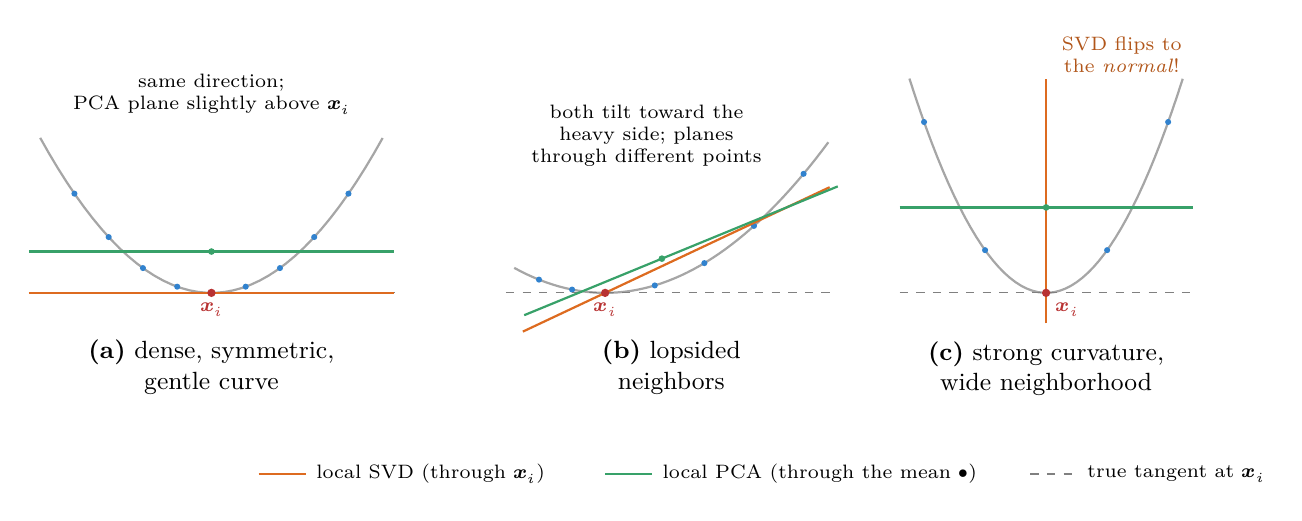
\begin{tikzpicture}
% ---------- (a) dense, symmetric, gentle curvature
\begin{scope}[x=2.9cm,y=7cm]
  \draw[thick, gray!70, domain=-0.75:0.75, samples=40] plot (\x,{0.5*\x*\x});
  \foreach \x in {-0.6,-0.45,-0.3,-0.15,0.15,0.3,0.45,0.6} \fill[dataC] (\x,{0.5*\x*\x}) circle (1.1pt);
  \draw[dashed, gray] (-0.8,0) -- (0.8,0);
  \draw[thick, accentC] (-0.8,0.0) -- (0.8,0.0);
  \draw[thick, accentD] (-0.8,0.075) -- (0.8,0.075);
  \fill[accentD] (0,0.075) circle (1.2pt);
  \fill[thmred] (0,0) circle (1.5pt) node[below, font=\scriptsize] {$\vx_i$};
  \node[font=\small, align=center] at (0,-0.135) {\textbf{(a)} dense, symmetric,\\gentle curve};
  \node[font=\scriptsize, align=center] at (0,0.36) {same direction;\\PCA plane slightly above $\vx_i$};
\end{scope}
% ---------- (b) lopsided
\begin{scope}[xshift=5.0cm, x=2.1cm,y=2.1cm]
  \draw[thick, gray!70, domain=-0.55:1.35, samples=50] plot (\x,{0.5*\x*\x});
  \foreach \x in {-0.4,-0.2,0.3,0.6,0.9,1.2} \fill[dataC] (\x,{0.5*\x*\x}) circle (1.1pt);
  \draw[dashed, gray] (-0.6,0) -- (1.4,0);
  \draw[thick, accentC] ({-0.55*0.905},{-0.55*0.426}) -- ({1.5*0.905},{1.5*0.426});
  \draw[thick, accentD] ({0.343-0.9*0.925},{0.207-0.9*0.380}) -- ({0.343+1.15*0.925},{0.207+1.15*0.380});
  \fill[accentD] (0.343,0.207) circle (1.2pt);
  \fill[thmred] (0,0) circle (1.5pt) node[below, font=\scriptsize] {$\vx_i$};
  \node[font=\small, align=center] at (0.4,-0.45) {\textbf{(b)} lopsided\\neighbors};
  \node[font=\scriptsize, align=center] at (0.25,0.95) {both tilt toward the\\heavy side; planes\\through different points};
\end{scope}
% ---------- (c) strong curvature, wide neighborhood
\begin{scope}[xshift=10.6cm, x=1.55cm,y=1.55cm]
  \draw[thick, gray!70, domain=-1.12:1.12, samples=50] plot (\x,{1.4*\x*\x});
  \foreach \x in {-1,-0.5,0.5,1} \fill[dataC] (\x,{1.4*\x*\x}) circle (1.1pt);
  \draw[dashed, gray] (-1.2,0) -- (1.2,0);
  \draw[thick, accentC] (0,-0.25) -- (0,1.75);
  \draw[thick, accentD] (-1.2,0.7) -- (1.2,0.7);
  \fill[accentD] (0,0.7) circle (1.2pt);
  \fill[thmred] (0,0) circle (1.5pt) node[below right, font=\scriptsize] {$\vx_i$};
  \node[font=\small, align=center] at (0,-0.62) {\textbf{(c)} strong curvature,\\wide neighborhood};
  \node[font=\scriptsize, align=center, accentC!80!black] at (0.62,1.95) {SVD flips to\\the \emph{normal}!};
\end{scope}
% legend
\begin{scope}[yshift=-2.3cm, xshift=0.6cm]
  \draw[thick, accentC] (0,0) -- (0.6,0) node[right, font=\scriptsize, black] {local SVD (through $\vx_i$)};
  \draw[thick, accentD] (4.4,0) -- (5.0,0) node[right, font=\scriptsize, black] {local PCA (through the mean $\bullet$)};
  \draw[dashed, gray] (9.8,0) -- (10.4,0) node[right, font=\scriptsize, black] {true tangent at $\vx_i$};
\end{scope}
\end{tikzpicture}
\caption{Local SVD vs.\ local PCA on three neighborhoods of the curve $y=c\,x^2$ at $\vx_i=(0,0)$, where the true tangent is horizontal.
Directions are the top singular vector / top loading computed from the plotted points. (Vertical scale exaggerated in (a).)}
\end{figure}

\begin{itemize}
\item \textbf{(a) Dense, symmetric, gently curved} ($c=\tfrac12$, nine points). Both methods return exactly the horizontal direction:
the left and right halves balance. The only difference is position: the PCA plane passes through the mean, which sits a
little \emph{above} $\vx_i$ because every point on a cup-shaped curve lies above its bottom. This is the ``results are
pretty similar'' regime.
\item \textbf{(b) Lopsided neighbors} (more points to the right). The neighborhood now covers a bent stretch of the curve, so
any best-fit line follows the chord of that stretch and tilts away from the tangent at $\vx_i$. Here the SVD direction is
$(0.905,0.426)$ and the PCA direction is $(0.925,0.380)$. The clearer difference is again \emph{where} the plane sits: the SVD
line is pinned at $\vx_i$ and cuts below most of the neighbors, while the PCA line runs through their middle.
\emph{(How the two tilts compare depends on the sample; with other lopsided samples they can come out nearly equal.)}
\item \textbf{(c) Strong curvature, wide neighborhood} ($c=1.4$, points at $x=\pm\tfrac12,\pm1$). This is where centering really matters. Centered
at $\vx_i$, every neighbor has a large positive height $y$, so ``up'' looks like the direction of greatest spread: the
uncentered second moments are $\sum x^2=2.5$ vs.\ $\sum y^2\approx4.2$, and the SVD picks the \emph{normal} direction $(0,1)$, a completely
wrong tangent. Centering at the mean removes the common height $\bar y=0.7$. What is left is variation \emph{around} the mean,
$\sum(y-\bar y)^2\approx1.7<2.5$, so PCA still picks the horizontal tangent $(1,0)$. Subtracting the mean takes the curvature-induced
offset out of the picture, which is the precise sense in which local PCA is less influenced by curvature.
\end{itemize}

\begin{intuition}
\textbf{The general pattern.} Curvature pushes every neighbor off the tangent plane \emph{to the same side} (into the cup).
Centering at $\vx_i$ treats that common offset as spread, and in the worst case as the main direction. Centering at the
mean subtracts the common offset first, leaving only the genuine spread along the manifold. The fix in every case is
also the same: use a smaller neighborhood (smaller $k$), so the patch is flatter and the offset shrinks relative to the
spread along the tangent. As the neighborhood shrinks, the curvature offset grows like (radius)$^2$ while the tangential spread
grows like (radius), so for small enough neighborhoods both methods find the tangent.
\end{intuition}

\subsubsection*{Both can fail: how, and what to do}

Both methods fit a \emph{flat} plane to a patch that is really curved, so they share most failure modes. Centering only
decides which one breaks first in a few cases.

\begin{center}
\renewcommand{\arraystretch}{1.35}
\small
\begin{tabular}{@{}>{\raggedright\arraybackslash}p{2.7cm}>{\raggedright\arraybackslash}p{5.4cm}>{\raggedright\arraybackslash}p{5.6cm}@{}}
\toprule
problem & what happens & example \\
\midrule
neighborhood too big & the patch is not flat; both fit a chord, and the scree plot shows too many dimensions & neighbors spread around a whole circle: $\lambda_1=\lambda_2=\tfrac12$, so ``$2$-D'' for a $1$-D curve (Example~\ref{ex:pcacircle}) \\
short-circuiting & the $k$ Euclidean-nearest points include points from a different part of $M$ & Swiss roll: a point on the next layer is close in $\R^3$ but far along the roll, so both estimates are garbage \\
too small / noisy & noise is as large as the real spread, so no clear scree gap; with $k\le t$ a $t$-dim plane cannot even be fit & points jittered off a curve: the normal direction gets as much variance as the tangent \\
sparse or uneven sampling & lopsided neighbors tilt both estimates toward the heavier side & case (b) of the figure above \\
\bottomrule
\end{tabular}
\end{center}

\textbf{Where they differ.}
\begin{itemize}[nosep]
\item \textbf{Local SVD fails first under curvature.} The common curvature offset counts as spread, and with enough
curvature the SVD flips to the \emph{normal} direction (case (c)). It is also more sensitive to noise \emph{at $\vx_i$ itself}, since
the whole plane is pinned to that single point.
\item \textbf{Local PCA's catch.} Its plane passes through the neighbors' \emph{mean}, not $\vx_i$, so it estimates the tangent near the
middle of the neighborhood, and $\vx_i$'s own local coordinate is not $(0,\dots,0)$. On a cup-shaped curve that mean lies off the manifold,
inside the cup.
\end{itemize}

\begin{careful}
\textbf{The common fix is choosing $k$ well.} Small enough that curvature is negligible (the offset shrinks like $r^2$, the tangent
spread like $r$), large enough that noise does not dominate and $k>t$. In practice, check that the scree gap is stable over a
range of $k$, and that the estimated $t$ agrees across many points. Local PCA is the safer default, but neither method
rescues a bad neighborhood.
\end{careful}

\subsubsection*{Reading the singular values: the zoom test}

\textbf{What a singular value measures.} Take $\vx_i$ and its $k$ neighbors, and draw the $k$ difference vectors
$\vx_{(j)}-\vx_i$ as arrows from $\vx_i$. Their tips form a small cloud.
\begin{itemize}[nosep]
\item $\sigma_1$ is how long that cloud is in its longest direction $\vv_1$;
\item $\sigma_2$ is how wide it is in the next direction $\vv_2$, perpendicular to the first;
\item $\sigma_3,\dots$ are its thickness in further perpendicular directions.
\end{itemize}
Precisely, $\sigma_j^2=\sum_{\ell=1}^k\big(\vv_j\T(\vx_{(\ell)}-\vx_i)\big)^2$, the total squared length of the arrows along $\vv_j$.
So $\sigma_2/\sigma_1$ is width $\div$ length, a measure of how fat the cloud is:
\begin{itemize}[nosep]
\item $\sigma_2/\sigma_1\approx0$: a thin streak. The neighbors line up, so locally the data look $1$-D.
\item $\sigma_2/\sigma_1$ near $1$: a round blob. The neighbors spread in two directions, so locally the data look $2$-D.
\end{itemize}
The raw $\sigma$'s grow with $k$ for two reasons: farther neighbors give longer arrows, and more neighbors give more
arrows to add up. The ratio cancels both, so it is the ratio that describes the \emph{shape}.

\textbf{Changing $k$ is zooming.} Small $k$ looks at a tiny patch, large $k$ at a big one.
\begin{itemize}[nosep]
\item \textbf{A sheet} (truly $2$-D). The neighbors fill a small disk. A disk of radius $r$ is $r$ long and $r$ wide, so the ratio stays
roughly the same at every zoom: both directions are real.
\item \textbf{A bent curve} (truly $1$-D). The neighbors lie on an arc of length $L$. An arc with curvature $\kappa$ sags sideways by only about
$\kappa L^2/2$, so width $\div$ length $\approx\kappa L/2$. Zoom in ($L\to0$) and the ratio goes to $0$: under a magnifying glass a bent
curve looks straight. (This is the same ``offset $\sim r^2$, spread $\sim r$'' fact as above.)
\end{itemize}

\begin{center}
\renewcommand{\arraystretch}{1.25}
\small
\begin{tabular}{@{}lll@{}}
\toprule
shape & zoomed out (large $k$) & zoomed in (small $k$) \\
\midrule
bent curve & fat-ish arc & thin line: $\sigma_2/\sigma_1\to0$ \\
sheet & round blob & round blob: $\sigma_2/\sigma_1$ stays put \\
\bottomrule
\end{tabular}
\end{center}

\begin{intuition}
\textbf{The rule.} A real dimension is still there no matter how closely you look. A bend disappears once you look closely enough.
\end{intuition}

\begin{figure}[htbp]
\centering
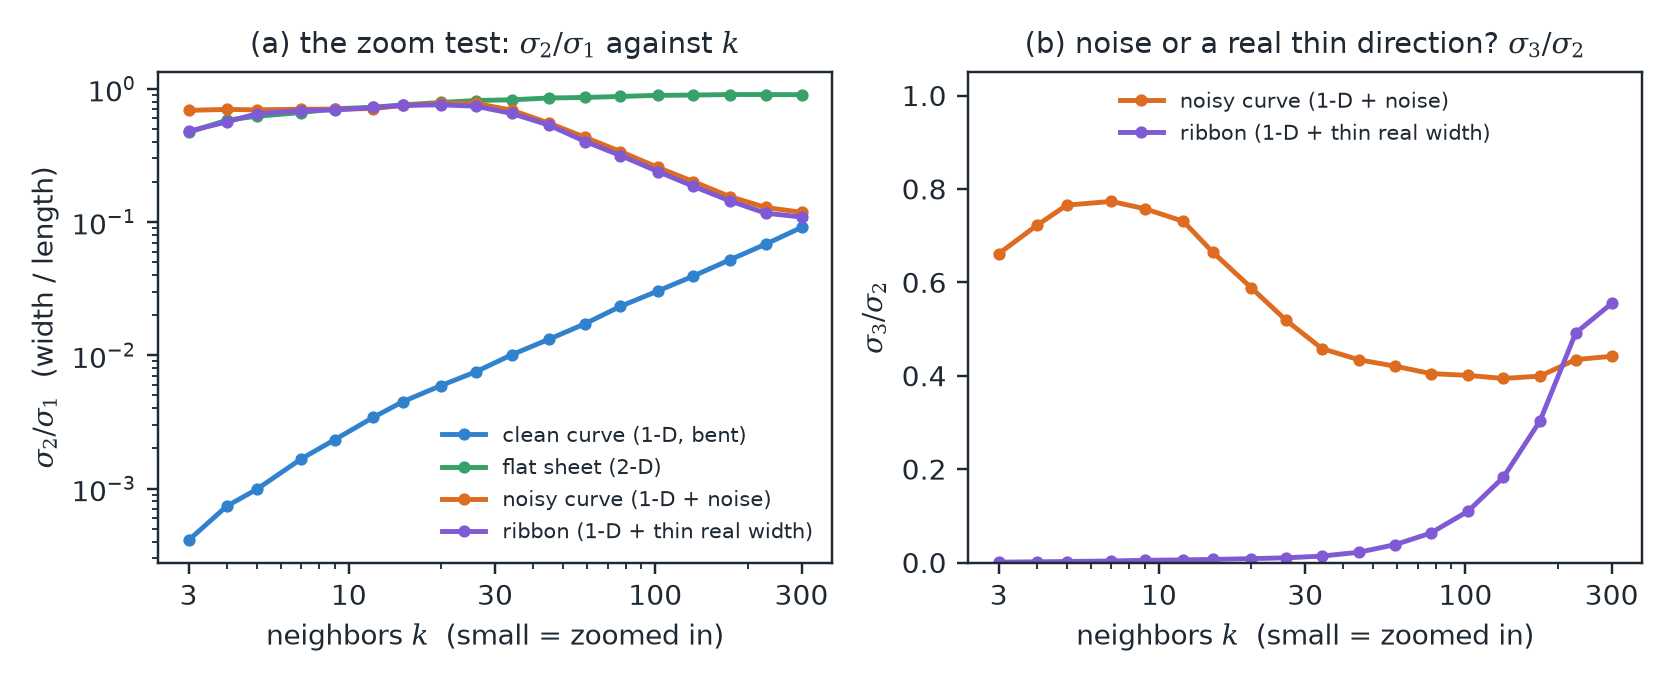
\includegraphics[width=\textwidth]{figures/zoom_test.png}
\caption{The zoom test on four shapes in $\R^{10}$ ($4000$ points each, local SVD at $150$ random base points, medians shown).
\textbf{(a)} $\sigma_2/\sigma_1$ against $k$. The clean curve (unit circle) falls steadily as you zoom in, from $0.09$ at $k=300$ to $0.0004$ at $k=3$.
The sheet stays high, between $0.7$ and $0.9$ for $k\ge7$. The noisy curve (noise sd $0.004$ in all $10$ coordinates) and the
ribbon (the circle thickened by $0.03$ in one extra direction) both fall like the curve at first, then level off near $0.7$ once the
patch is as small as the noise or the width. \textbf{(b)} $\sigma_3/\sigma_2$ tells those two apart: at $k\le12$ it is $0.66$ to $0.77$ for
the noisy curve but below $0.01$ for the ribbon. (Figures from \texttt{figures/zoom\_figures.py}.)}
\label{fig:zoomtest}
\end{figure}

\begin{careful}
\textbf{Three things the simple rule leaves out} (Figure~\ref{fig:zoomtest}).
\begin{enumerate}[nosep,label=\arabic*)]
\item \textbf{Anything of fixed size stops the fall.} Noise of size $\varepsilon$, or a real but thin second direction of width $w$, adds a
width that does not shrink when you zoom. Width $\div$ length is then about $(\kappa L^2+w)/L$: it falls like a bend while $L\gg w$,
then levels off (or rises) once $L$ is comparable to $w$. So the evidence for a second dimension is a ratio that \emph{stops falling},
not one that is merely above $0$ at the smallest $k$ you tried.
\item \textbf{Noise and a thin real direction look the same in $\sigma_2/\sigma_1$.} Look one singular value further. Noise spreads
equally into every direction off the manifold, so $\sigma_2\approx\sigma_3\approx\cdots$ and $\sigma_3/\sigma_2$ is large. A real thin direction sticks
out alone, so $\sigma_3\ll\sigma_2$ (panel (b)).
\item \textbf{Very small $k$ biases the ratio down.} With only $k$ arrows the cloud is lopsided by chance. Even for the flat sheet,
the median $\sigma_2/\sigma_1$ is $0.47$ at $k=3$, against $0.73$ at $k=12$. So a drop at the smallest $k$ is partly a small-sample effect; compare
with what a genuine sheet gives at the same $k$.
\end{enumerate}
\end{careful}

\begin{example}{Reading a zoom test}{zoomread}
Suppose $\sigma_2/\sigma_1$ goes $0.44\to0.40\to0.32\to0.23$ as $k$ drops from $12$ to $3$. It shrinks as you zoom in, which is the bent-curve pattern,
and it is well below what a sheet gives at the same $k$ ($0.73$ at $k=12$, $0.47$ at $k=3$ in Figure~\ref{fig:zoomtest}). The leftover $0.23$ is not by
itself evidence for a second dimension: the ratio is still falling at the smallest $k$, so it may simply not have been zoomed in far
enough (for example, if consecutive samples are as close as the data allow). An argument for $2$-D would need the ratio to level
off as $k$ shrinks, together with $\sigma_3/\sigma_2$ well below $1$, showing one real extra direction rather than noise in all of them.
\end{example}

\subsection{Geodesic distance and isometry}

\textbf{Two ways to measure distance} between $\vx_1,\vx_2\in M$:
\begin{enumerate}[nosep,label=\arabic*)]
\item \textbf{Euclidean:} $\norm{\vx_1-\vx_2}$, the straight line through the ambient space, which ignores the manifold.
\item \textbf{Geodesic:} restrict movement to the manifold, and measure arc length along $M$.
\end{enumerate}

\begin{definition}{Geodesic distance}{geodesic}
For $\vx_1,\vx_2\in M$, let $C(\vx_1,\vx_2)$ be the set of all smooth paths $\gamma:[0,1]\to M$ with $\gamma(0)=\vx_1$, $\gamma(1)=\vx_2$ (smooth meaning
differentiable as many times as needed). The \textbf{geodesic distance} is the length of the shortest such path:
\[
d^M(\vx_1,\vx_2)=\inf_{\gamma\in C(\vx_1,\vx_2)}\int_0^1\Big\|\frac{d\gamma}{ds}\Big\|\,ds .
\]
\end{definition}

\begin{intuition}
$\norm{d\gamma/ds}$ is the speed of a traveler along the path, so the integral is the total distance traveled, and the
infimum asks for the shortest route that never leaves the surface: an ant crawling on $M$ rather than a bird flying
through $\R^d$. Always $d^M(\vx_1,\vx_2)\ge\norm{\vx_1-\vx_2}$, since the straight line is the shortest path of all. On the Swiss roll two points on
adjacent layers can be very close in Euclidean distance but far apart geodesically: the ant must go all the way
around the spiral. That gap is exactly what PCA (and classical MDS on Euclidean distances) gets wrong.
\end{intuition}

\begin{example}{Geodesics on the helix}{helixgeo}
For the unit-speed helix $\psi(s)=\tfrac1{\sqrt2}(\cos s,\ \sin s,\ s)$, the curve itself is the only path between two of its points, and its speed
is $1$ (Example~\ref{ex:helixtangent}), so
\[
d^M\big(\psi(s_1),\psi(s_2)\big)=\int_{s_1}^{s_2}1\,ds=|s_1-s_2| ,
\]
which is exactly the distance between the parameters $s_1,s_2$. The $\tfrac1{\sqrt2}$ normalization is what makes this work.
\end{example}

\begin{definition}{Isometry}{isometry}
A manifold map $\psi:A\to M$ is an \textbf{isometry} if it preserves geodesic distances:
\[
d^M\big(\psi(\bm s),\psi(\bm t)\big)=d^A(\bm s,\bm t)\qquad\text{for all }\bm s,\bm t\in A .
\]
If $A$ is \textbf{convex}, the straight segment between any two points stays inside $A$, so $d^A(\bm s,\bm t)=\norm{\bm s-\bm t}$.
\end{definition}

\begin{example}{Isometry or not?}{isoex}
\begin{itemize}[nosep]
\item \textbf{Helix:} an isometry, by the example above.
\item \textbf{Swiss roll:} \emph{not} an isometry. It stretches distances in the $y_1$ direction by $\sqrt{1+y_1^2}$ (the length of the first
Jacobian column, Example~\ref{ex:srtangent}), more and more as it winds outward.
\end{itemize}
\end{example}

\begin{definition}{Local isometry}{localiso}
$\psi:A\to M$ is a \textbf{local isometry} if every $\bm y\in A$ has a neighborhood $U$ such that $\psi$ restricted to $U$ is an isometry.
\end{definition}

\begin{proposition}{Isometry $\Rightarrow$ local isometry, but not conversely}{isolocal}
Every isometry is a local isometry. The converse fails: $\psi:\R^2\to\R^3$, $\psi(s,t)=(\cos s,\ \sin s,\ t)$ wraps the plane onto a cylinder and is
a local isometry but not an isometry.
\end{proposition}
\begin{proofsketch}
Local: $J_\psi=\begin{bmatrix}-\sin s&0\\\cos s&0\\0&1\end{bmatrix}$ has orthonormal columns, so small pieces of the plane are rolled onto the cylinder
without stretching. Not global: $\psi(0,t)=\psi(2\pi,t)$, so $d^M\big(\psi(0,t),\psi(2\pi,t)\big)=0$ while $d^A\big((0,t),(2\pi,t)\big)=2\pi$.
\end{proofsketch}

\begin{example}{The cylinder on an open strip: local isometry, not an isometry}{cylhw}
Let $C=\{(x,y,z)\in\R^3\mid x^2+y^2=1\}$ and $F:\R\times(0,2\pi)\to C$, $F(u,v)=(\cos v,\ \sin v,\ u)$, with $\R\times(0,2\pi)$ regarded as a subset
of the Euclidean plane $\R^2$. (Here $u$ is the height and $v$ the angle, the reverse of the board's $(s,t)$.)

\textbf{(a) $F$ is a local isometry.} $J_F=\Big[\frac{\partial F}{\partial u}\ \ \frac{\partial F}{\partial v}\Big]=\begin{bmatrix}0&-\sin v\\0&\cos v\\1&0\end{bmatrix}$. The columns have length $1$ and
dot product $0$, so $J_F\T J_F=I_2$ and Proposition~\ref{prop:jaciso} applies. Geometrically, $F$ rolls a strip of paper into a tube
without stretching it.

\textbf{(b) $F$ is not an isometry.} The tempting argument ``$v=0$ and $v=2\pi$ land on the same point'' does not work
here, because \emph{both are excluded}: the domain uses the open interval $(0,2\pi)$, which makes $F$ one-to-one. Use points
that \emph{are} in the domain, just close to the edges: $\bm p=(0,\varepsilon)$ and $\bm q=(0,2\pi-\varepsilon)$ for small $\varepsilon>0$.
\begin{itemize}[nosep]
\item In the plane: $d^A(\bm p,\bm q)=|(2\pi-\varepsilon)-\varepsilon|=2\pi-2\varepsilon\approx2\pi$.
\item On the cylinder: $F(\bm p)=(\cos\varepsilon,\ \sin\varepsilon,\ 0)$ and $F(\bm q)=(\cos\varepsilon,\ -\sin\varepsilon,\ 0)$, two points on the unit circle at height $0$
separated by angle $2\varepsilon$. The shortest path along $C$ is an arc of length $2\varepsilon$, so $d^C\big(F(\bm p),F(\bm q)\big)=2\varepsilon$. (The straight line
in $\R^3$ is even shorter, $2\sin\varepsilon$.)
\end{itemize}
Points about $2\pi$ apart in the domain land almost on top of each other, so $F$ does not preserve distances globally.
\emph{A second reason:} $F$ is not surjective. It never reaches the seam $\{(1,0,u):u\in\R\}$, where $v=0$. An isometry \emph{between}
$\R\times(0,2\pi)$ and $C$ would have to be a bijection, so this alone rules it out.
\end{example}

\begin{intuition}
\textbf{Local vs.\ global, in one picture.} Locally $F$ just rolls up the strip, so short lengths are preserved (part (a)).
Globally the strip wraps around, and its two long edges, far apart in the plane, are brought next to each other along
the seam. A local isometry can only be checked by looking at small steps (the Jacobian), but an isometry must also respect
how far apart \emph{distant} points are, and wrapping breaks that.
\end{intuition}

\begin{proposition}{Jacobian test for local isometry}{jaciso}
$\psi$ is a local isometry if $J_\psi$ has orthonormal columns at every point, i.e.\ $J_\psi\T J_\psi=I_t$.
\end{proposition}
\begin{proofsketch}
A short step $\bm\delta$ in $A$ moves the image by $\approx J_\psi\bm\delta$, and $\norm{J_\psi\bm\delta}^2=\bm\delta\T J_\psi\T J_\psi\bm\delta=\norm{\bm\delta}^2$. So every small
step keeps its length, and so does every path built from small steps.
\end{proofsketch}

\begin{intuition}
Picture rolling a sheet of paper into a tube: no tearing, no stretching, so locally everything is the same as on the flat
sheet (local isometry), but globally two points on opposite edges of the sheet have been glued together. The Swiss
roll fails the Jacobian test because its first column has length $\sqrt{1+s^2}\ne1$, even though its two columns are
orthogonal. Orthogonal columns alone are not enough; they must also be unit length.
\end{intuition}

\subsubsection*{Gluing the edges: allowed, but it changes global distances}

Is it ``cheating'' to glue two edges of the sheet together? No. Gluing is exactly what turns a sheet into a cylinder, and the
result is a perfectly good manifold. But it is worth being precise about what changes and what does not.

\begin{figure}[htbp]
\centering
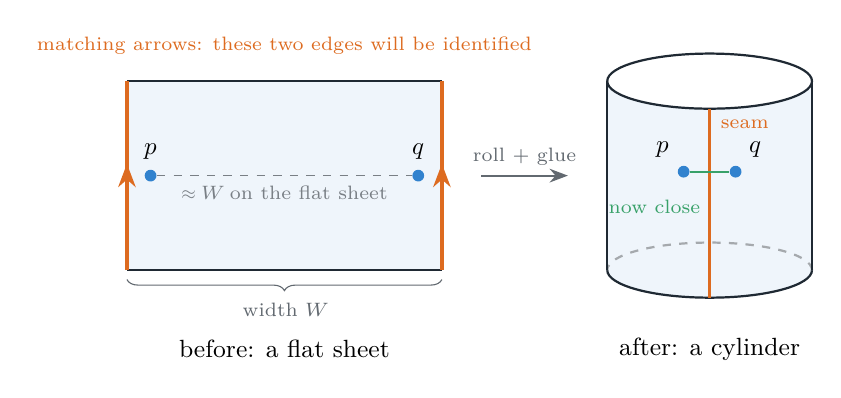
\begin{tikzpicture}[>=Stealth,
  pt/.style={circle,fill=#1,inner sep=1.5pt}]
% ---------- flat sheet ----------
\begin{scope}
\fill[dataC!8] (0,0) rectangle (4,2.4);
\draw[thick,ink] (0,0) -- (4,0) (0,2.4) -- (4,2.4);
\draw[very thick,accentC,->] (0,0) -- (0,1.35); \draw[very thick,accentC] (0,1.2) -- (0,2.4);
\draw[very thick,accentC,->] (4,0) -- (4,1.35); \draw[very thick,accentC] (4,1.2) -- (4,2.4);
\node[pt=dataC,label={[font=\small]above:$p$}] (p) at (0.3,1.2) {};
\node[pt=dataC,label={[font=\small]above:$q$}] (q) at (3.7,1.2) {};
\draw[dashed,ink!60] (p) -- (q) node[midway,below,font=\scriptsize]{$\approx W$ on the flat sheet};
\draw[decorate,decoration={brace,mirror,amplitude=4pt},ink!70] (0,-0.12) -- (4,-0.12) node[midway,below=5pt,font=\scriptsize]{width $W$};
\node[font=\small] at (2,-1.0) {before: a flat sheet};
\node[font=\scriptsize,accentC,align=center] at (2,2.85) {matching arrows: these two edges will be identified};
\end{scope}
% ---------- arrow ----------
\draw[->,thick,ink!70] (4.5,1.2) -- (5.6,1.2) node[midway,above,font=\scriptsize]{roll + glue};
% ---------- cylinder ----------
\begin{scope}[xshift=7.4cm,yshift=0cm]
\fill[dataC!8] (-1.3,0) -- (-1.3,2.4) arc[start angle=180,end angle=360,x radius=1.3,y radius=0.35] -- (1.3,0) arc[start angle=0,end angle=-180,x radius=1.3,y radius=0.35];
\draw[thick,ink] (0,2.4) ellipse (1.3 and 0.35);
\draw[thick,ink] (-1.3,0) arc[start angle=180,end angle=360,x radius=1.3,y radius=0.35];
\draw[thick,ink,dashed,ink!40] (1.3,0) arc[start angle=0,end angle=180,x radius=1.3,y radius=0.35];
\draw[thick,ink] (-1.3,0) -- (-1.3,2.4) (1.3,0) -- (1.3,2.4);
% seam (front, at angle -90)
\draw[very thick,accentC] (0,-0.35) -- (0,2.05);
\node[font=\scriptsize,accentC,right] at (0.02,1.85) {seam};
\node[pt=dataC,label={[font=\small]above left:$p$}] (p2) at (-0.33,1.25) {};
\node[pt=dataC,label={[font=\small]above right:$q$}] (q2) at (0.33,1.25) {};
\draw[thick,accentD] (p2) -- (q2);
\node[font=\scriptsize,accentD,align=center] at (-0.7,0.8) {now close};
\node[font=\small] at (0,-1.0) {after: a cylinder};
\end{scope}
\end{tikzpicture}
\caption{Rolling the sheet and gluing its left and right edges. Nothing is stretched, so small neighborhoods look exactly as before.
But $p$ and $q$, about $W$ apart on the flat sheet, end up next to each other across the seam.}
\label{fig:glue}
\end{figure}

\begin{intuition}
\textbf{What is preserved and what is not.}
\begin{itemize}[nosep,leftmargin=*]
\item \textbf{Local geometry is preserved.} Rolling does not stretch or tear the paper. Short lengths and angles are unchanged, which is the
Jacobian test $J\T J=I$ of Proposition~\ref{prop:jaciso}. The gluing does not spoil this, because the seam itself is flat too. A small disk
straddling the seam is two half-disks from opposite edges, and they fit together into an ordinary flat disk.
\item \textbf{Global distances are not.} Gluing creates a \emph{shortcut} across the seam. Write a point of the cylinder by its arc-length coordinate
$a\in[0,W)$ around the tube and its height $h$. The shortest path on the cylinder is a straight line on the sheet, except that it may now exit
one edge and re-enter at the other:
\[
d^{C}\big((a_1,h_1),(a_2,h_2)\big)=\sqrt{\min\big(|a_1-a_2|,\ W-|a_1-a_2|\big)^2+(h_1-h_2)^2}.
\]
The $\min$ is the only change from the flat formula. For $p,q$ in Figure~\ref{fig:glue}, $|a_1-a_2|\approx W$, so the distance drops from
$\approx W$ to almost $0$.
\item \textbf{The topology changes too.} A glued rectangle is not the same space as a rectangle. It has a loop that cannot be shrunk to a point (once around
the tube), and it has lost two of its four edges.
\end{itemize}
This is the content of Example~\ref{ex:cylhw}(b) seen from the paper's side: the map is a local isometry but not an isometry, because the seam
connects points that were far apart.
\end{intuition}

\begin{careful}
\begin{itemize}[nosep,leftmargin=*]
\item \textbf{The shortcut only exists after gluing.} If you roll the sheet only part of the way, so its edges do not meet, the rolled sheet with
its own intrinsic distance is \emph{globally} isometric to the flat sheet. Every path on it unrolls to a path on the flat sheet of the same length, and
there is no seam to cut across. The loss of global isometry comes from the \emph{identification} of edges, not from the bending.
\item \textbf{The torus needs a qualifier.} Gluing both pairs of opposite edges gives a torus. Abstractly, this \emph{flat torus} is locally
Euclidean everywhere. But the doughnut you draw in $\R^3$ is \emph{not} a rolled-up sheet of paper: its outer equator is longer than its inner one,
so the paper would have to stretch on the outside and squash on the inside. That is why the torus is described as ``doughnut-shaped \emph{topologically}.''
(The flat torus does sit isometrically in $\R^4$, as $(\cos\alpha,\sin\alpha,\cos\beta,\sin\beta)$, with each factor a cylinder-style roll.)
\end{itemize}
\end{careful}

\begin{deeper}
\textbf{Why manifold learning cares.} Isomap assumes the manifold is isometric to a convex region of $\R^t$ (Section~\ref{sec:isomap}). A closed
cylinder violates this: no flat map of it can keep both the short distance across the seam and the long distance the other way around. Isomap
has to tear the loop open or bend it, and its geodesic matrix shows this as negative eigenvalues in classical scaling. The circle is the
1-D version: its intrinsic dimension is $1$, but any faithful picture of it needs $2$ coordinates. Laplacian eigenmaps handles this naturally. On a ring
of $N$ points the smoothest non-constant eigenvectors are $\cos(2\pi i/N)$ and $\sin(2\pi i/N)$, so $[\vv_2\ \vv_3]$ draws the ring as a circle
(Section~\ref{sec:laplacian}). Local information is kept, and the global loop is shown honestly rather than torn.
\end{deeper}

\subsection{Isomap: isometric mapping}\label{sec:isomap}

Isomap turns the three-step plan into an algorithm: approximate geodesic distances with a neighborhood graph, then
hand them to classical scaling (Chapter~6).

\begin{algorithm}{Isomap}{isomap}
\begin{enumerate}[label=\arabic*)]
\item \textbf{Neighborhood graph.} Fix $k\in\{1,2,\dots\}$ (or a radius $\varepsilon>0$). Compute all Euclidean distances $d_{ij}=\norm{\vx_i-\vx_j}$ and use them to
decide which points are nearest neighbors. Build a weighted graph with one vertex per data point and edge weights
\[
E_{ij}=\begin{cases}d_{ij}&\text{if $i$ is among $j$'s $k$ nearest neighbors, or $j$ among $i$'s},\\ \infty&\text{otherwise.}\end{cases}
\]
(The ``or'' makes the graph symmetric, since nearest-neighbor relations need not be mutual.)
\item \textbf{Graph-based (geodesic) distances.} Estimate the geodesic distance by the shortest path through the graph,
summing Euclidean lengths of short hops:
\[
d^M(\vx_i,\vx_j)\approx d^G(\vx_i,\vx_j)=\min_{\text{paths }i\to j}\ \sum_{\text{edges }(a,b)\text{ on the path}}d_{ab} ,
\]
computed by Dijkstra's algorithm from every vertex (about $O(N^2\log N)$) or Floyd--Warshall. Collect them in the matrix
$D^G$, $D^G_{ij}=d^G(\vx_i,\vx_j)$.
\item \textbf{Classical scaling on $D^G$.} For $t=1,2,\dots$ find $\bm y_1,\dots,\bm y_N\in\R^t$ with $\norm{\bm y_i-\bm y_j}\approx d^G(\vx_i,\vx_j)$: form
$B=-\tfrac12H(D^G\had D^G)H$ and take the top $t$ eigenpairs (Algorithm~\ref{alg:classical}).
\end{enumerate}
\end{algorithm}

\begin{figure}[htbp]
\centering
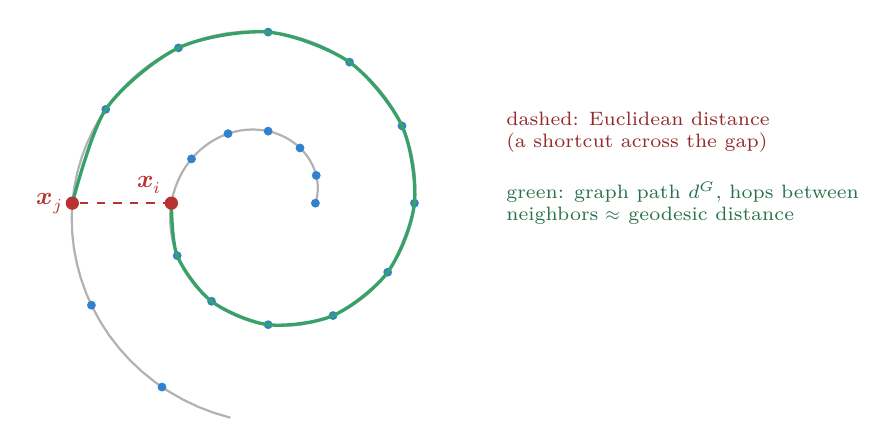
\begin{tikzpicture}[scale=1.0]
  \draw[thick, gray!60, domain=0:620, samples=140, variable=\a] plot ({(0.6+0.0035*\a)*cos(\a)},{(0.6+0.0035*\a)*sin(\a)});
  \foreach \a in {0,30,...,600} \fill[dataC] ({(0.6+0.0035*\a)*cos(\a)},{(0.6+0.0035*\a)*sin(\a)}) circle (1.6pt);
  \coordinate (P) at ({(0.6+0.0035*180)*cos(180)},{(0.6+0.0035*180)*sin(180)});
  \coordinate (Q) at ({(0.6+0.0035*540)*cos(540)},{(0.6+0.0035*540)*sin(540)});
  \draw[accentD, very thick] plot[smooth] coordinates {
    ({(0.6+0.0035*180)*cos(180)},{(0.6+0.0035*180)*sin(180)}) ({(0.6+0.0035*210)*cos(210)},{(0.6+0.0035*210)*sin(210)})
    ({(0.6+0.0035*240)*cos(240)},{(0.6+0.0035*240)*sin(240)}) ({(0.6+0.0035*270)*cos(270)},{(0.6+0.0035*270)*sin(270)})
    ({(0.6+0.0035*300)*cos(300)},{(0.6+0.0035*300)*sin(300)}) ({(0.6+0.0035*330)*cos(330)},{(0.6+0.0035*330)*sin(330)})
    ({(0.6+0.0035*360)*cos(360)},{(0.6+0.0035*360)*sin(360)}) ({(0.6+0.0035*390)*cos(390)},{(0.6+0.0035*390)*sin(390)})
    ({(0.6+0.0035*420)*cos(420)},{(0.6+0.0035*420)*sin(420)}) ({(0.6+0.0035*450)*cos(450)},{(0.6+0.0035*450)*sin(450)})
    ({(0.6+0.0035*480)*cos(480)},{(0.6+0.0035*480)*sin(480)}) ({(0.6+0.0035*510)*cos(510)},{(0.6+0.0035*510)*sin(510)})
    ({(0.6+0.0035*540)*cos(540)},{(0.6+0.0035*540)*sin(540)})};
  \draw[thmred, thick, dashed] (P) -- (Q);
  \fill[thmred] (P) circle (2.4pt) node[above left, font=\small] {$\vx_i$};
  \fill[thmred] (Q) circle (2.4pt) node[left, font=\small] {$\vx_j$};
  \node[thmred!80!black, font=\scriptsize, align=left, anchor=west] at (2.9,0.9) {dashed: Euclidean distance\\(a shortcut across the gap)};
  \node[accentD!70!black, font=\scriptsize, align=left, anchor=west] at (2.9,0.0) {green: graph path $d^G$, hops between\\neighbors $\approx$ geodesic distance};
\end{tikzpicture}
\caption{Geodesic distance estimated by a shortest path through the neighborhood graph. Euclidean distance cuts straight
across between turns of the spiral; the graph path has to follow the curve.}
\end{figure}

\begin{proposition}{Graph distances converge to geodesics}{graphgeo}
With dense enough sampling (and $k$ or $\varepsilon$ chosen suitably), $d^G(\vx_i,\vx_j)\to d^M(\vx_i,\vx_j)$ as $N\to\infty$.
\end{proposition}

\begin{intuition}
Euclidean distance is trusted only over short hops, where the manifold is nearly flat and Euclidean $\approx$ geodesic
(the same assumption as local PCA). Chaining many short hops connects distant points through intermediate
neighbors, so the path is forced to follow the surface, the ant hopping from neighbor to neighbor. More samples
give shorter hops and a path that hugs the manifold more tightly.
\end{intuition}

\subsubsection*{Assumptions, and why they make it work}

\begin{enumerate}[label=\arabic*)]
\item \textbf{Isometry.} The data are images $\vx_i=\psi(\bm y_i)$, $i=1,\dots,N$, of an isometry $\psi:A\to M$.
\item \textbf{Convexity.} The set $A\subseteq\R^t$ is convex, so the shortest distance between two of its points is the straight line.
\end{enumerate}
Together they give the chain that justifies step 3:
\[
\underbrace{\norm{\bm y_i-\bm y_j}}_{\text{Euclidean in }A}\ \overset{\text{convexity}}{=}\ d^A(\bm y_i,\bm y_j)\ \overset{\text{isometry}}{=}\ d^M(\vx_i,\vx_j)\ \approx\ d^G(\vx_i,\vx_j) .
\]
So the graph distances are (approximately) \emph{Euclidean distances of the latent points}, which is exactly the input classical
scaling can invert.

\begin{careful}
\textbf{Convexity is about $A$, not $M$.} The latent set $A\subseteq\R^t$ must be convex. The manifold $M\subseteq\R^d$ need not be: the Swiss
roll and the helix are far from convex, yet Isomap works on them, because their parameter sets are a rectangle and an
interval. A latent set with a hole (an annulus, say) breaks the chain: straight lines in $A$ would cut through the
hole, so $\norm{\bm y_i-\bm y_j}<d^A(\bm y_i,\bm y_j)$ and the geodesic distances are no longer Euclidean distances of any configuration.
\end{careful}

\textbf{Estimating the intrinsic dimension.} With enough samples and the assumptions met, the doubly centered matrix
\[
B=-\tfrac12H\big(D^G\had D^G\big)H
\]
is (nearly) the Gram matrix of $\bm y_1,\dots,\bm y_N\in\R^t$, so its rank, the number of non-zero eigenvalues (in practice, the number of large
ones in a scree plot), reveals $t$. Midterm note from lecture: classical scaling and the rank of this matrix are fair game.

\textbf{Seeing a short-circuit.} Everything rests on the graph following the manifold. One neighborhood size too large is enough to break that (Figure~\ref{fig:shortcircuit}).

\begin{figure}[htbp]
\centering
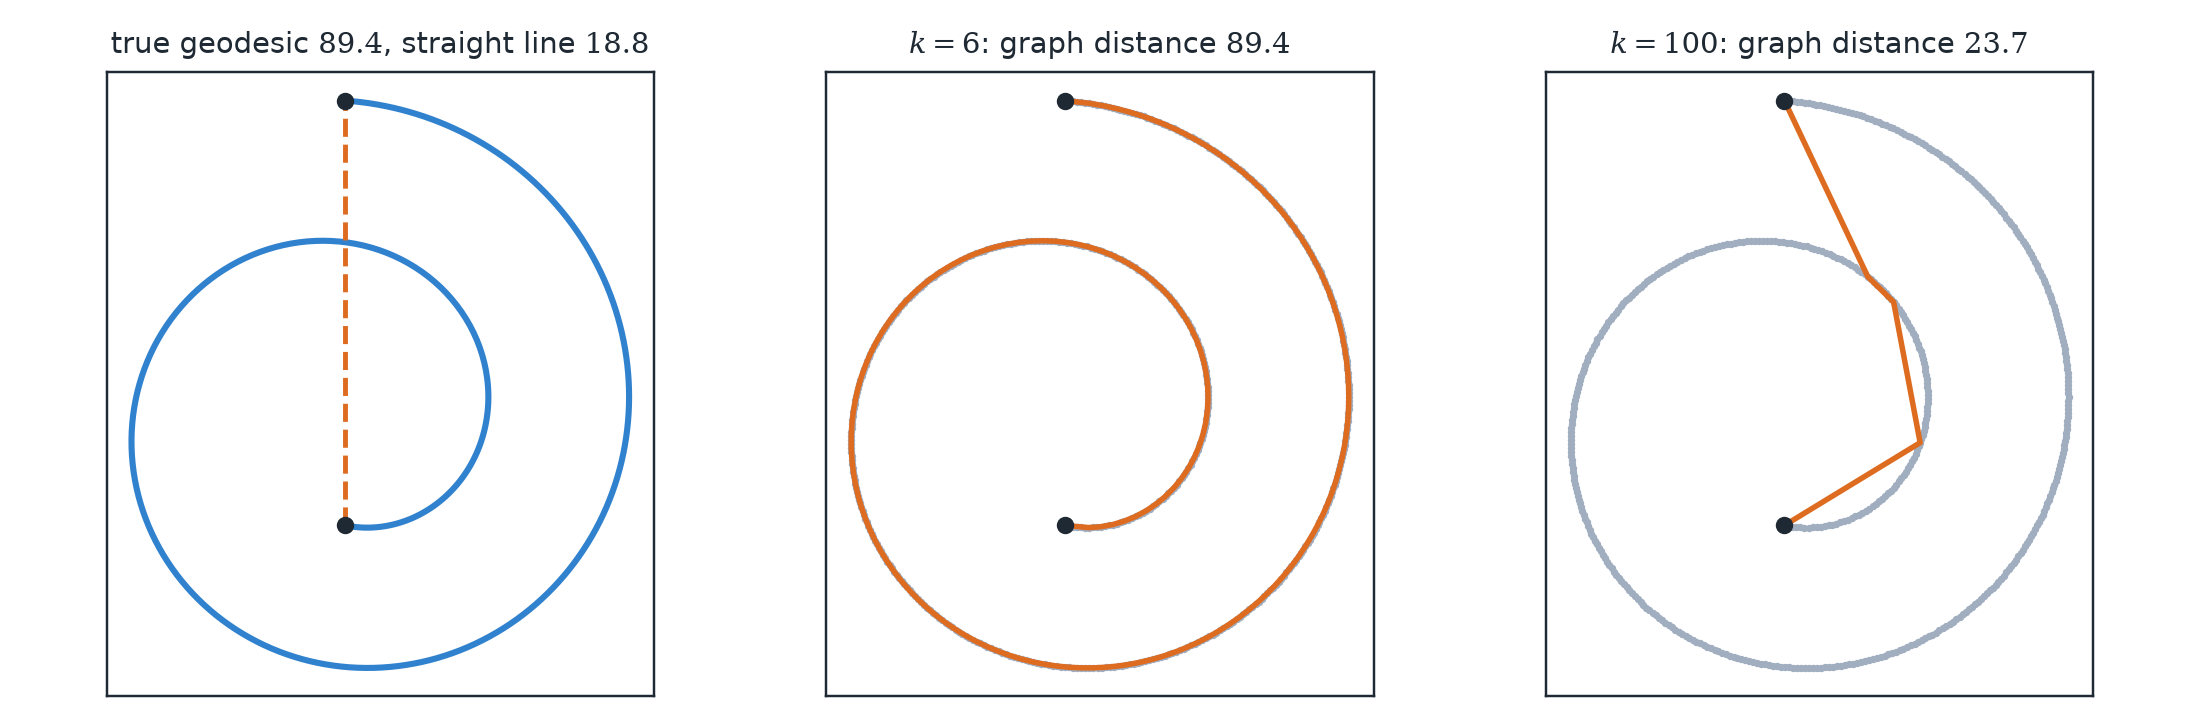
\includegraphics[width=\textwidth]{figures/iso_shortcircuit.png}
\caption{$500$ points on a spiral, with the shortest graph path between its ends in orange. With $k=6$, the path follows the curve and gets the geodesic right ($89.4$). With $k=100$, the neighborhoods are wide enough to jump between layers (the longest hop is $8.65$, while the layers are about $2\pi$ apart), and the estimate collapses to $23.7$, close to the straight-line $18.8$.}
\label{fig:shortcircuit}
\end{figure}

\subsubsection*{Strengths and weaknesses}

\begin{center}
\renewcommand{\arraystretch}{1.3}
\small
\begin{tabular}{@{}>{\raggedright\arraybackslash}p{6.6cm}>{\raggedright\arraybackslash}p{7.2cm}@{}}
\toprule
strengths & weaknesses \\
\midrule
\textbf{Global structure.} When the assumptions hold and $d^G=d^M$, Isomap recovers $\norm{\bm y_i-\bm y_j}=d^M(\vx_i,\vx_j)$ for \emph{all} pairs, not just neighbors. &
\textbf{Strong assumptions and dense sampling} (isometry, convex $A$). Sparse sampling causes \textbf{shortcuts}: a neighbor edge jumps across a gap of the manifold and collapses distances. \\
\textbf{Somewhat robust} to small deviations from isometry: mild stretching (as in the Swiss roll) still gives qualitatively correct coordinates. &
\textbf{No out-of-sample extension:} a new point means rerunning on the whole data set. \textbf{Cost:} the $N\times N$ eigendecomposition is $O(N^3)$. \\
\textbf{Closed-form final step:} an eigendecomposition, no iterative optimization or local optima. &
\textbf{Noise:} sensitive in theory, though averaging over many short hops helps in practice. \textbf{Disconnected graph} ($k$ too small): some $d^G=\infty$. \\
\bottomrule
\end{tabular}
\end{center}

\begin{deeper}
\textbf{Landmark Isomap} handles the out-of-sample and cost problems: compute graph distances only to a small set of
landmark points, embed the landmarks by classical scaling, then place every other point (old or new) by
triangulating from its distances to the landmarks. The lecture flagged it as a strong final-paper topic. Note also
that Isomap is ``kernel PCA with a geodesic kernel'': $B=-\tfrac12H(D^G\had D^G)H$ plays the role of $HKH$ (Section~\ref{sec:kpca}),
except that $B$ need not be PSD when the assumptions fail, which shows up as negative eigenvalues.
\end{deeper}

\subsection{Graph Laplacian and Laplacian eigenmaps}\label{sec:laplacian}

\begin{definition}{Weighted graph, affinity and degree matrices}{affinity}
Let $G=(V,E)$ be an undirected graph on vertices $1,\dots,N$ with weights $E_{ij}=0$ if $i,j$ are not connected and $E_{ij}>0$ if
they are. A larger $E_{ij}$ means a stronger connection. The \textbf{affinity matrix} $A\in\R^{N\times N}$ stores all the weights,
\[
A_{ij}=E_{ij}\ (i\ne j),\qquad A_{ii}=0 .
\]
The \textbf{degree matrix} $D\in\R^{N\times N}$ is diagonal with the row sums of $A$: $D_{ii}=(A\one_N)_i=\sum_{j=1}^NA_{ij}$, the total connection strength of vertex $i$.
(This $D$ is unrelated to a distance matrix.)
\end{definition}

\begin{definition}{Graph Laplacian}{laplacian}
\[
L=D-A=\begin{bmatrix}\sum_jA_{1j}&-A_{12}&\cdots&-A_{1N}\\-A_{21}&\sum_jA_{2j}&\cdots&-A_{2N}\\\vdots&&\ddots&\vdots\\-A_{N1}&-A_{N2}&\cdots&\sum_jA_{Nj}\end{bmatrix}.
\]
For Laplacian eigenmaps the weights come from data, e.g.\ $A_{ij}=e^{-\norm{\vx_i-\vx_j}^2/\sigma^2}$ (an RBF kernel) if $i,j$ are neighbors and $0$ otherwise.
\end{definition}

\begin{theorem}{Properties of the graph Laplacian}{lapprops}
\begin{enumerate}[nosep,label=(\roman*)]
\item $L$ is \textbf{symmetric} (since $A$ is), so it is diagonalizable with orthonormal eigenvectors (spectral theorem).
\item For every $\bm y=(y_1,\dots,y_N)\T\in\R^N$:
$\ \displaystyle\bm y\T L\bm y=\tfrac12\sum_{i=1}^N\sum_{j=1}^NA_{ij}(y_i-y_j)^2\ \ge0$, so $L$ is \textbf{PSD} with eigenvalues $0=\lambda_1\le\lambda_2\le\cdots\le\lambda_N$.
\item $\one_N$ is an eigenvector of $L$ with eigenvalue $0$.
\item For vectors $\bm y_1,\dots,\bm y_N\in\R^t$ stacked as the rows of $Y=\begin{bmatrix}\bm y_1\T\\\vdots\\\bm y_N\T\end{bmatrix}$:
$\ \displaystyle\tfrac12\sum_{i=1}^N\sum_{j=1}^NA_{ij}\norm{\bm y_i-\bm y_j}^2=\tr(Y\T LY)$.
\end{enumerate}
\end{theorem}
\begin{proofsketch}
(ii) $\bm y\T L\bm y=\bm y\T D\bm y-\bm y\T A\bm y=\sum_iD_{ii}y_i^2-\sum_{i,j}A_{ij}y_iy_j=\sum_{i,j}A_{ij}y_i^2-\sum_{i,j}A_{ij}y_iy_j$. Splitting the first sum into two halves
and using $A_{ij}=A_{ji}$ to rename indices in one of them gives $\tfrac12\sum_{i,j}A_{ij}(y_i^2+y_j^2-2y_iy_j)=\tfrac12\sum_{i,j}A_{ij}(y_i-y_j)^2$. Every term has $A_{ij}\ge0$
times a square. (iii) $(L\one)_i=D_{ii}-\sum_jA_{ij}=0$: each row of $L$ sums to zero. (iv) Apply (ii) to each column of $Y$ and add:
$\tr(Y\T LY)=\sum_{c=1}^t Y_{:c}\T LY_{:c}$, and $\sum_c(Y_{ic}-Y_{jc})^2=\norm{\bm y_i-\bm y_j}^2$.
\end{proofsketch}

\begin{example}{A three-vertex path}{lappath}
Vertices $1-2-3$ with unit weights: $A=\begin{bmatrix}0&1&0\\1&0&1\\0&1&0\end{bmatrix}$, $D=\diag(1,2,1)$, $L=\begin{bmatrix}1&-1&0\\-1&2&-1\\0&-1&1\end{bmatrix}$.
Eigenpairs: $0$ with $(1,1,1)$, $1$ with $(1,0,-1)$, $3$ with $(1,-2,1)$. Check (ii) with $\bm y=(1,0,-1)$: $\tfrac12\cdot2\big[(1-0)^2+(0+1)^2\big]=2=\bm y\T L\bm y$.
The smoothest non-constant vector, $(1,0,-1)$, simply orders the vertices along the path.
\end{example}

\textbf{Part (ii) again, slowly, from the definition of matrix multiplication.} Scalars commute, so
\[
\bm y\T L\bm y=\sum_{i=1}^N\sum_{j=1}^Ny_iL_{ij}y_j=\sum_{i,j}L_{ij}y_iy_j .
\]
With no self-loops ($A_{ii}=0$), $L=D-A$ has $L_{ii}=D_{ii}=\sum_jA_{ij}$ and $L_{ij}=-A_{ij}$ for $i\ne j$. Now separate the diagonal from the rest:
\[
\bm y\T L\bm y=\underbrace{\sum_iL_{ii}y_i^2}_{\text{diagonal}}+\underbrace{\sum_{i\ne j}L_{ij}y_iy_j}_{\text{off-diagonal}}
=\sum_i\Big(\sum_jA_{ij}\Big)y_i^2-\sum_{i\ne j}A_{ij}y_iy_j .
\]
Collect everything that involves one edge $\{i,j\}$. The diagonal gives $A_{ij}y_i^2$ (inside $D_{ii}$) and $A_{ij}y_j^2$ (inside $D_{jj}$). The off-diagonal gives $-A_{ij}y_iy_j$ twice, from entries $(i,j)$ and $(j,i)$. Together:
\[
A_{ij}\big(y_i^2+y_j^2-2y_iy_j\big)=A_{ij}(y_i-y_j)^2,
\qquad\text{so}\qquad
\bm y\T L\bm y=\sum_{i<j}A_{ij}(y_i-y_j)^2=\tfrac12\sum_{i,j}A_{ij}(y_i-y_j)^2 .
\]
The $\tfrac12$ is there only because $\sum_{i,j}$ visits each edge twice. On the path $1-2-3$ with $\bm y=(3,1,2)\T$, here are the nine numbers $y_iL_{ij}y_j$, colored by which edge they belong to. The middle diagonal entry $2y_2^2$ splits between the two edges, because vertex $2$ has degree $2$:
\[
\big[y_iL_{ij}y_j\big]=\begin{bmatrix}\textcolor{dataC}{9}&\textcolor{dataC}{-3}&0\\\textcolor{dataC}{-3}&\textcolor{dataC}{1}+\textcolor{accentC}{1}&\textcolor{accentC}{-2}\\0&\textcolor{accentC}{-2}&\textcolor{accentC}{4}\end{bmatrix},
\qquad
\begin{aligned}
\textcolor{dataC}{\text{edge }1{-}2:}&\ \ 9+1-3-3=4=(3-1)^2,\\
\textcolor{accentC}{\text{edge }2{-}3:}&\ \ 1+4-2-2=1=(1-2)^2.
\end{aligned}
\]
All nine entries add to $5=4+1$, the sum of squared differences across the edges.

\begin{example}{Reading $L$ on a weighted graph}{lapanatomy}
Take four vertices with the values $\bm y=(1,1,2,4)\T$ written on them:
\begin{center}
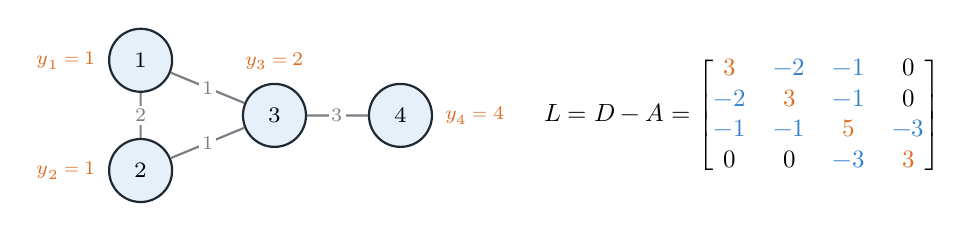
\begin{tikzpicture}[v/.style={circle,draw=ink,thick,fill=dataC!12,minimum size=8mm,inner sep=0pt,font=\footnotesize},w/.style={font=\scriptsize,fill=white,inner sep=1pt}]
\node[v] (a) at (0,1.3) {$1$}; \node[v] (b) at (0,-0.1) {$2$}; \node[v] (c) at (1.7,0.6) {$3$}; \node[v] (d) at (3.3,0.6) {$4$};
\draw[thick,ink!60] (a)--node[w]{$2$}(b) (a)--node[w]{$1$}(c) (b)--node[w]{$1$}(c) (c)--node[w]{$3$}(d);
\node[font=\scriptsize,accentC,left=1pt] at (a.west) {$y_1=1$}; \node[font=\scriptsize,accentC,left=1pt] at (b.west) {$y_2=1$};
\node[font=\scriptsize,accentC,above=1pt] at (c.north) {$y_3=2$}; \node[font=\scriptsize,accentC,right=1pt] at (d.east) {$y_4=4$};
\node[anchor=west] at (5.0,0.6) {\small$L=D-A=
\begin{bmatrix}\textcolor{accentC}{3}&\textcolor{dataC}{-2}&\textcolor{dataC}{-1}&0\\\textcolor{dataC}{-2}&\textcolor{accentC}{3}&\textcolor{dataC}{-1}&0\\\textcolor{dataC}{-1}&\textcolor{dataC}{-1}&\textcolor{accentC}{5}&\textcolor{dataC}{-3}\\0&0&\textcolor{dataC}{-3}&\textcolor{accentC}{3}\end{bmatrix}$};
\end{tikzpicture}
\end{center}
\textbf{Diagonal:} the total weight touching a vertex (\textcolor{accentC}{orange}). \textbf{Off-diagonal:} minus the weight of an edge (\textcolor{dataC}{blue}); $0$ means no edge. Every row sums to $0$.

\textbf{Row $i$ of $L\bm y$ compares a vertex with its neighbors:} $(L\bm y)_i=\sum_jA_{ij}(y_i-y_j)$. Here $L\bm y=(-1,-1,-4,6)\T$. For example, vertex $4$ gets $3\cdot(4-2)=6$: positive, since it sits above its neighbor. Vertex $3$ gets $1\cdot(2-1)+1\cdot(2-1)+3\cdot(2-4)=-4$: negative, since its heavy neighbor is above it.

\textbf{$\bm y\T L\bm y$ adds up one penalty per edge}, each one weight $\times$ (difference)$^2$:
\begin{center}
\small
\renewcommand{\arraystretch}{1.2}
\begin{tabular}{lcccc|c}
\toprule
edge & $1\text{--}2$ & $1\text{--}3$ & $2\text{--}3$ & $3\text{--}4$ & total\\
\midrule
$A_{ij}(y_i-y_j)^2$ & $2\cdot0^2=0$ & $1\cdot1^2=1$ & $1\cdot1^2=1$ & $3\cdot2^2=12$ & $14$\\
\bottomrule
\end{tabular}
\end{center}
The direct product agrees: $\bm y\T L\bm y=1(-1)+1(-1)+2(-4)+4(6)=14$. The heavy edge with a big difference dominates, which is exactly what minimizing is meant to punish.
\end{example}

\begin{intuition}
\textbf{$\bm y\T L\bm y$ measures roughness.} It adds up $A_{ij}(y_i-y_j)^2$ over connected pairs, so it is small when strongly connected
vertices get similar values. Using vertex values as coordinates, \emph{minimizing} $\tr(Y\T LY)$ pulls together points with large $A_{ij}$:
large $A_{ij}$ forces small $\norm{\bm y_i-\bm y_j}$. That is the whole idea of Laplacian eigenmaps: find low-dimensional coordinates in
which neighbors on the graph stay neighbors. The constant vector $\one$ achieves roughness $0$ trivially (every point at the same
place), which is why the problem has to be a \textbf{constrained optimization}. \textbf{Spectral graph theory} uses $L$ for
much more, e.g.\ clustering: the number of zero eigenvalues equals the number of connected components of the graph.
\end{intuition}

\begin{careful}
\textbf{Eigenvector of $L$, not of $A$.} It is easy to write ``$\one_N$ is an eigenvector of $A$'' by accident. It is an eigenvector of
$L$ with eigenvalue $0$, because every row of $L$ sums to zero. For $A$ itself, $A\one_N=(D_{11},\dots,D_{NN})\T$ is the vector of degrees,
so $\one_N$ is an eigenvector of $A$ only when every vertex has the same degree.
\end{careful}

\subsubsection*{Eigenvectors are the graph's vibration modes}

Since $\bm y\T L\bm y$ measures roughness, the eigenvectors of $L$ sort vertex values from smoothest to roughest. For a unit eigenvector, $\bm v\T L\bm v=\lambda$, so \textbf{the eigenvalue is the roughness} (Figure~\ref{fig:roughness}).

\begin{figure}[htbp]
\centering
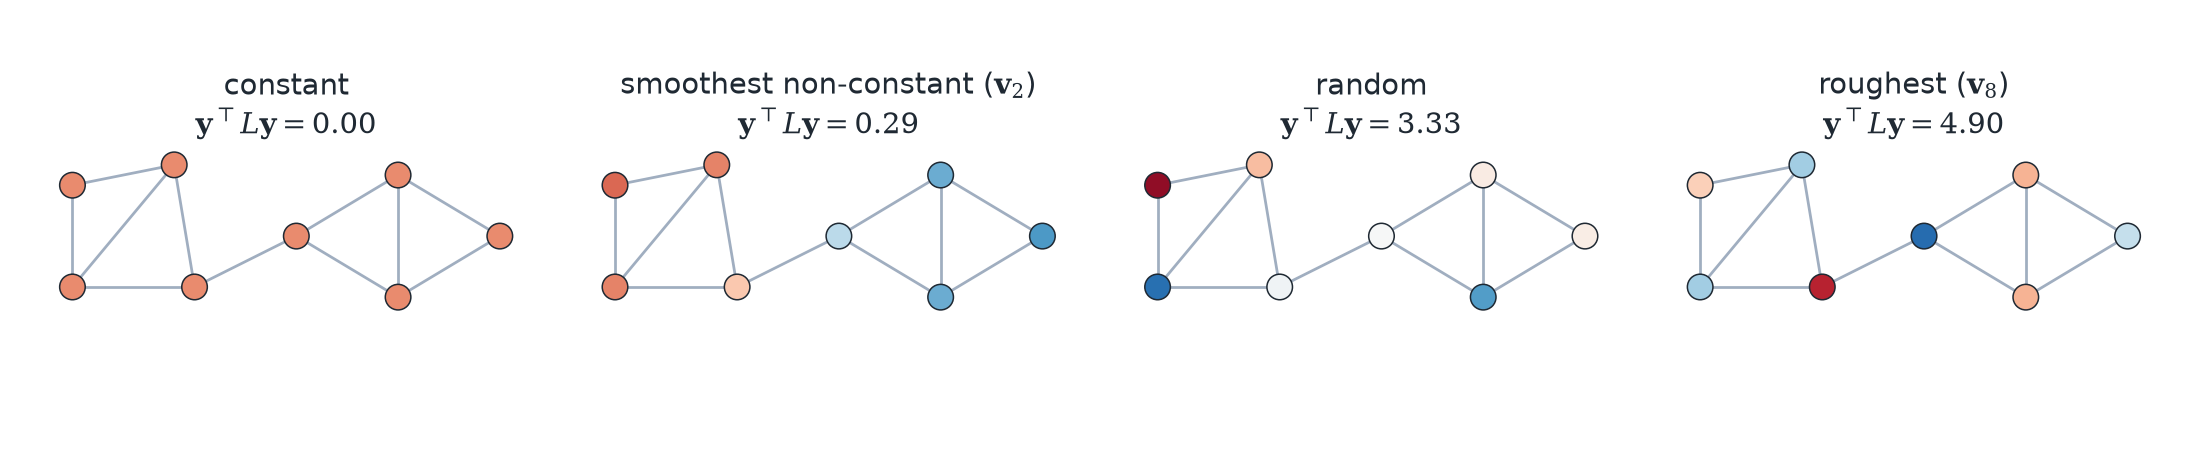
\includegraphics[width=\textwidth]{figures/lap_roughness.png}
\caption{Four unit-length assignments of values to the same graph (red is positive, blue negative). The roughness runs from $0$ for the constant, through $0.29$ for $\bm v_2$, which simply splits the graph at its narrow bridge, up to the maximum $4.90$ for $\bm v_8$, which makes neighbors disagree as much as it can.}
\label{fig:roughness}
\end{figure}

Think of the graph as a network of masses joined by springs. Its eigenvectors are the shapes in which it vibrates, slow and smooth first, and they look like the waves of a plucked string (Figure~\ref{fig:modes}). These smooth waves are what Laplacian eigenmaps uses as coordinates.

\begin{figure}[htbp]
\centering
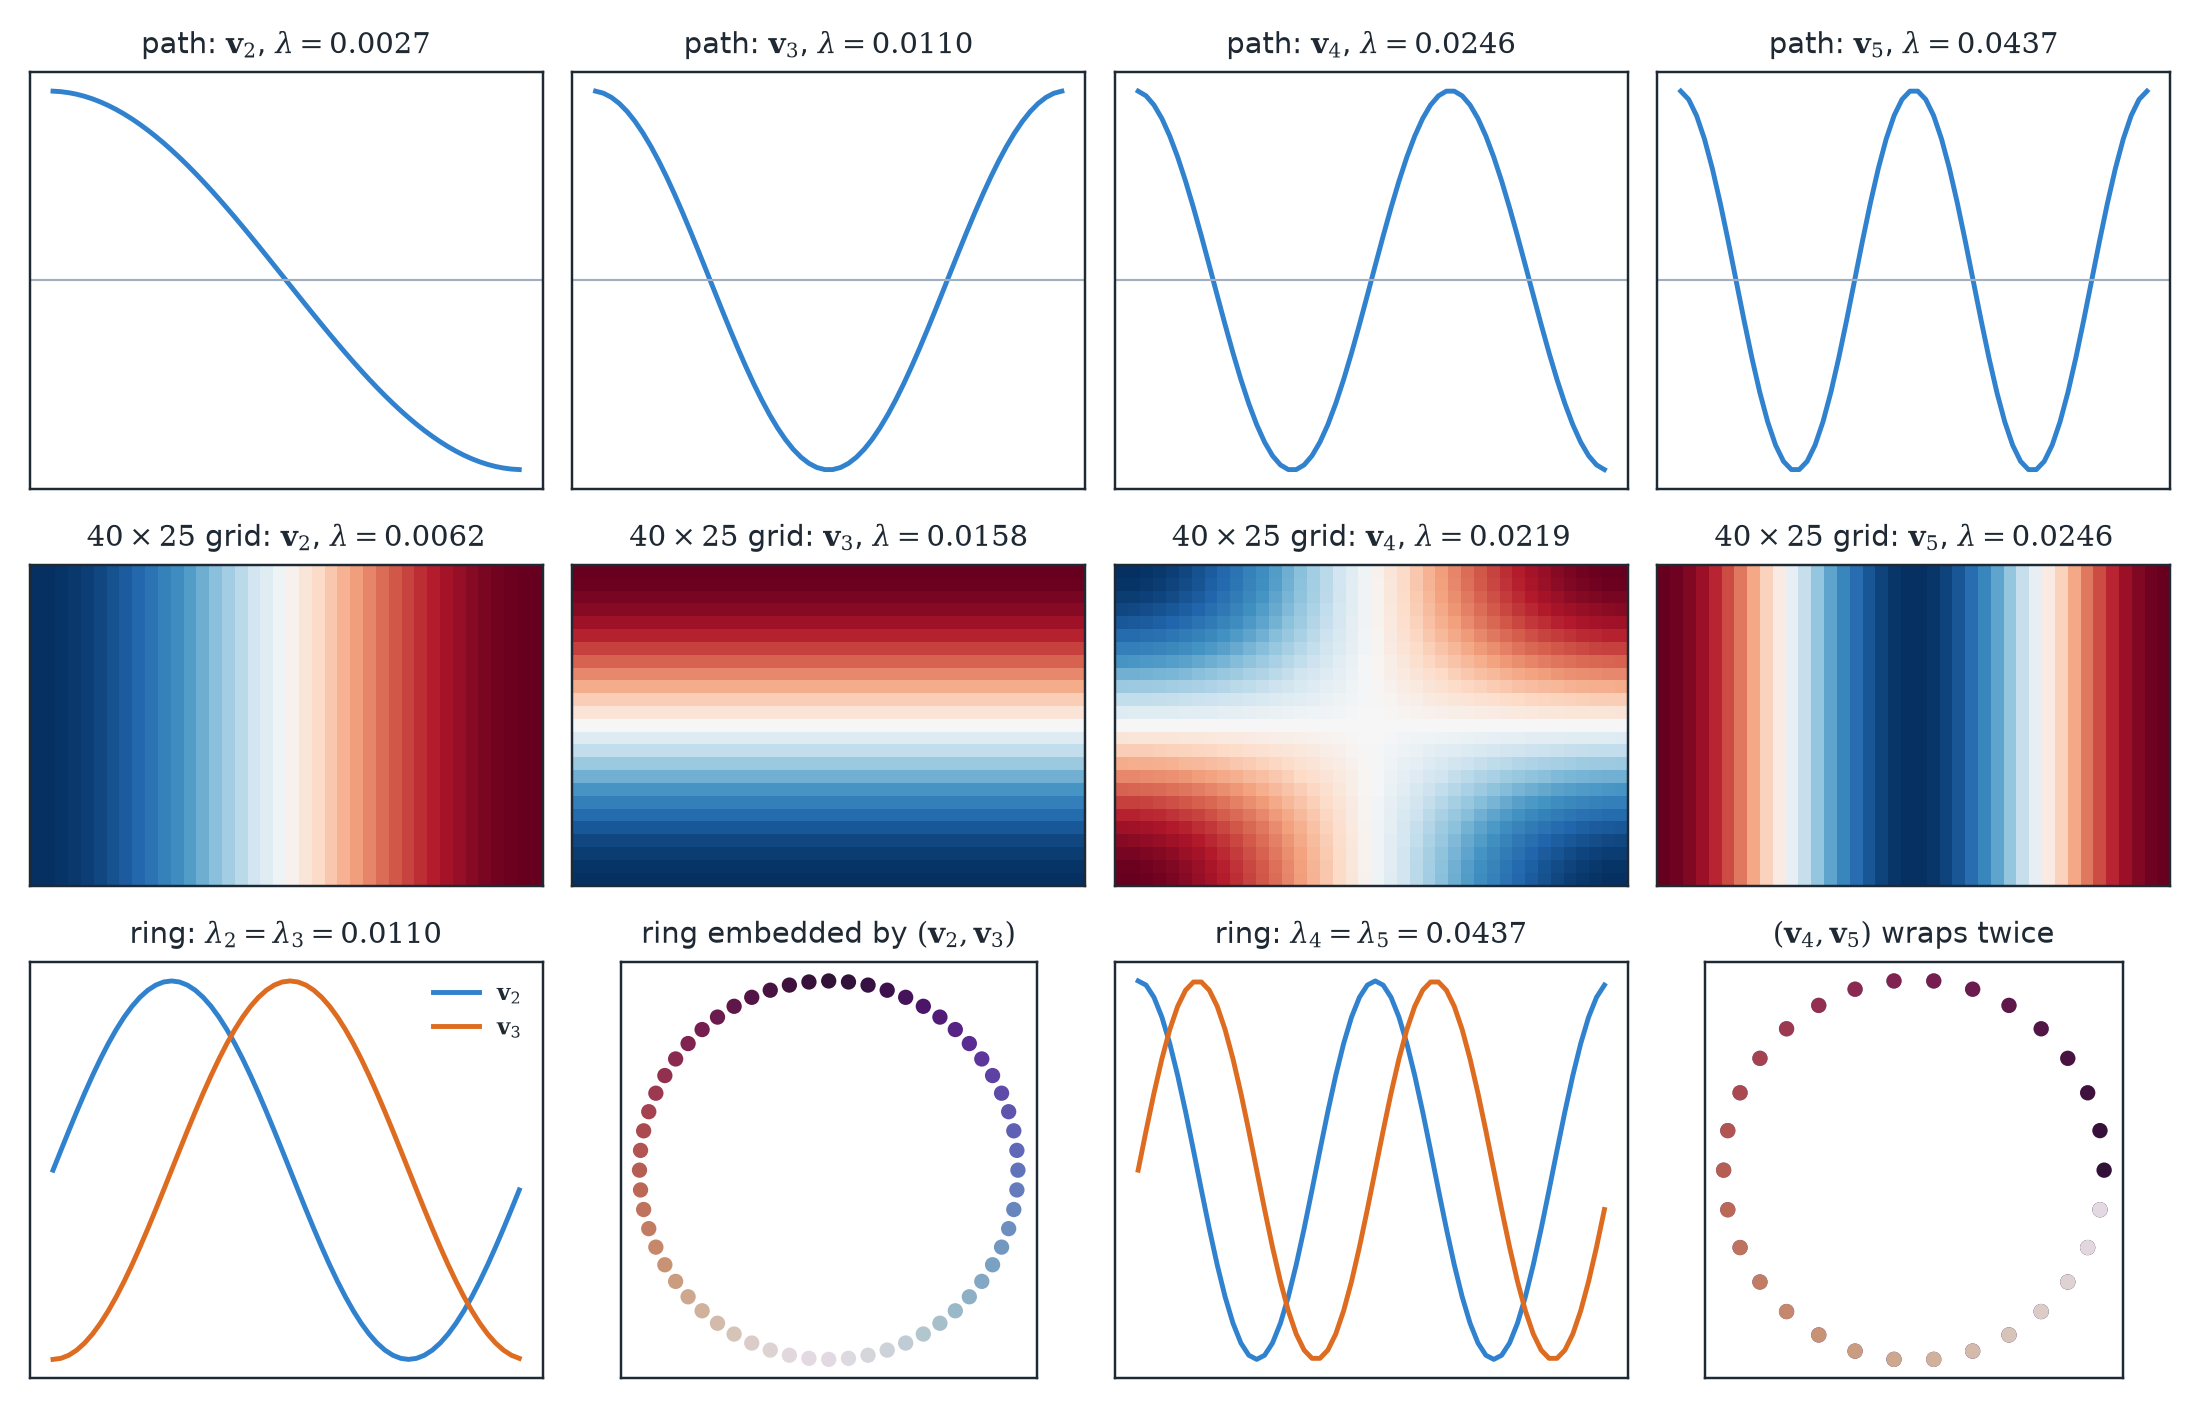
\includegraphics[width=\textwidth]{figures/lap_modes.png}
\caption{Eigenvectors of $L$ on three simple graphs. \emph{Path:} cosine waves, where $\bm v_j$ changes sign $j-1$ times. \emph{Grid:} $\bm v_2$ is one wave along the long side, and $\bm v_3$ one along the short side. Waves along the long side cost less, so a second one ($\bm v_5$) arrives before many waves across. \emph{Ring:} with no ends, eigenvalues come in equal pairs of sine and cosine, and $(\bm v_2,\bm v_3)$ draws the ring as a circle. This is the claim made at the end of the gluing discussion in Section~\ref{sec:manifold}. $(\bm v_4,\bm v_5)$ goes around twice, so it is a poor coordinate system, even though it is also a circle.}
\label{fig:modes}
\end{figure}

\subsubsection*{The algorithm, step 1: build a neighbor graph}

The vertices are the data points, $V=\{1,\dots,N\}$ with vertex $i$ standing for $\vx_i$. Two standard ways to draw edges:
\begin{itemize}[nosep]
\item \textbf{$\varepsilon$-ball graph.} Choose $\varepsilon>0$. Connect $i$ and $j$ if $\norm{\vx_i-\vx_j}\le\varepsilon$.
\item \textbf{$k$-nearest-neighbor graph.} Choose $k\in\{1,2,\dots\}$. Connect $i$ and $j$ if $\vx_j$ is one of the $k$ nearest neighbors of $\vx_i$
\emph{or} $\vx_i$ is one of the $k$ nearest neighbors of $\vx_j$.
\end{itemize}
Let $N_i$ be the set of points that $\vx_i$ is connected to. The ``or'' matters: ``$j$ is among $i$'s $k$ nearest'' is not a symmetric relation, and
the ``or'' symmetrizes it, so $j\in N_i\iff i\in N_j$ and the graph is undirected.

\begin{figure}[htbp]
\centering
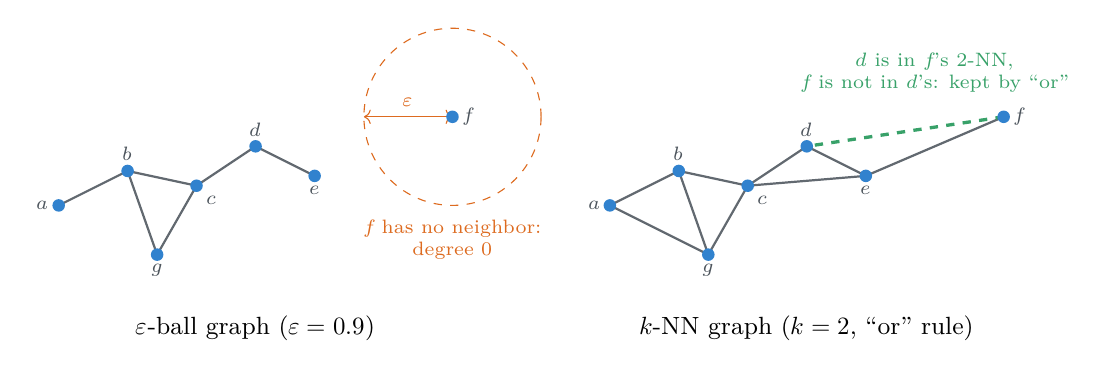
\begin{tikzpicture}[scale=1.25,
  pt/.style={circle,fill=dataC,inner sep=1.6pt},
  ed/.style={thick,ink!70},
  lab/.style={font=\scriptsize,ink!80}]
% ---------- epsilon graph ----------
\begin{scope}
\coordinate (a) at (0,0); \coordinate (b) at (0.7,0.35); \coordinate (c) at (1.4,0.2);
\coordinate (d) at (2.0,0.6); \coordinate (e) at (2.6,0.3); \coordinate (f) at (4.0,0.9); \coordinate (g) at (1.0,-0.5);
\draw[ed] (a)--(b) (b)--(c) (c)--(d) (d)--(e) (g)--(c) (g)--(b);
\draw[dashed,accentC] (f) circle (0.9);
\draw[<->,accentC,thin] (f) -- ++(-0.9,0) node[midway,above,font=\scriptsize]{$\varepsilon$};
\foreach \p in {a,b,c,d,e,f,g} \node[pt] at (\p) {};
\foreach \p/\pos in {a/left,b/above,c/below right,d/above,e/below,f/right,g/below} \node[lab,\pos] at (\p) {$\p$};
\node[font=\small] at (2,-1.25) {$\varepsilon$-ball graph ($\varepsilon=0.9$)};
\node[font=\scriptsize,accentC,align=center] at (4.0,-0.35) {$f$ has no neighbor:\\ degree $0$};
\end{scope}
% ---------- kNN graph ----------
\begin{scope}[xshift=5.6cm]
\coordinate (a) at (0,0); \coordinate (b) at (0.7,0.35); \coordinate (c) at (1.4,0.2);
\coordinate (d) at (2.0,0.6); \coordinate (e) at (2.6,0.3); \coordinate (f) at (4.0,0.9); \coordinate (g) at (1.0,-0.5);
\draw[ed] (a)--(b) (a)--(g) (b)--(c) (c)--(d) (d)--(e) (e)--(c) (g)--(c) (g)--(b) (f)--(e);
\draw[ed,accentD,very thick,dashed] (f)--(d);
\foreach \p in {a,b,c,d,e,f,g} \node[pt] at (\p) {};
\foreach \p/\pos in {a/left,b/above,c/below right,d/above,e/below,f/right,g/below} \node[lab,\pos] at (\p) {$\p$};
\node[font=\small] at (2,-1.25) {$k$-NN graph ($k=2$, ``or'' rule)};
\node[font=\scriptsize,accentD,align=center] at (3.3,1.35) {$d$ is in $f$'s 2-NN,\\ $f$ is not in $d$'s: kept by ``or''};
\end{scope}
\end{tikzpicture}
\caption{The same seven points under the two rules. The $\varepsilon$-ball graph leaves the outlier $f$ isolated (degree $0$, so $D$ is not invertible
and the graph is disconnected). The $k$-NN graph gives every point at least $k$ neighbors. Points can get \emph{more} than $k$ (here $c$ has four),
because the ``or'' rule adds every point that picked them.}
\label{fig:epsknn}
\end{figure}

\subsubsection*{Step 2: weights and the graph Laplacian}

Put an RBF (heat-kernel) weight on each edge and zero elsewhere:
\[
A_{ij}=\begin{cases}e^{-\norm{\vx_i-\vx_j}^2/\sigma^2}, & j\in N_i,\\ 0, & \text{otherwise,}\end{cases}
\qquad D=\diag(A\one_N),\qquad L=D-A .
\]
$A$ is symmetric because the neighbor relation is. Row $i$ of $A$ has only $|N_i|$ non-zero entries. For a $k$-NN graph that is at least $k$
(and usually close to $k$), so when $k$ or $\varepsilon$ is small, $A$ and $L$ are \textbf{sparse}: about $Nk$ non-zeros instead of $N^2$.

\begin{intuition}
\textbf{Sparse on purpose: kernel PCA with the far-away entries deleted.} The weight formula is exactly the RBF kernel from kernel PCA (Section~\ref{sec:kpca}). The difference is what happens to far-apart pairs.
Kernel PCA keeps every $K_{ij}$, so far points still talk to each other through a dense $N\times N$ matrix. Laplacian eigenmaps sets those
entries to exactly $0$, so a pair of points interacts only if they are graph neighbors. That has two effects. Computation is cheap, because sparse
eigen-solvers only ever multiply by $L$. And the method is \emph{local}: two points that are close in $\R^d$ but far apart along the
manifold (the two layers of a Swiss roll) are not neighbors once $k$ or $\varepsilon$ is small enough, so they have no direct pull on each other.
\end{intuition}

\subsubsection*{Step 3: the constrained optimization}

Theorem~\ref{thm:lapprops}(iv) turns ``keep strongly connected points close'' into a trace. Minimizing it alone fails, so two constraints are added:
\[
\boxed{\begin{aligned}
Y=\begin{bmatrix}\bm y_1\T\\\vdots\\\bm y_N\T\end{bmatrix}&=\argmin_{Y\in\R^{N\times t}}\ \tr(Y\T LY)=\argmin_{Y\in\R^{N\times t}}\ \tfrac12\sum_{i=1}^N\sum_{j=1}^NA_{ij}\norm{\bm y_i-\bm y_j}^2\\
&\text{subject to}\quad Y\T D\one_N=\bm0\ \ (\text{``centering''}),\qquad Y\T DY=I_t\ \ (\text{``scaling''}).
\end{aligned}}
\]

\textbf{The core problem: the loss only pulls, it never pushes.} Every term of $\sum_{i,j}A_{ij}\norm{\bm y_i-\bm y_j}^2$ says ``bring these two points closer,'' and no term says ``keep these two apart.'' So the loss cannot tell ``preserved the local structure'' from ``threw all the information away.'' Figure~\ref{fig:pullonly} shows this on the chain $A-B-C$ with $A_{AB}=A_{BC}=1$, $A_{AC}=0$ and $D=\diag(1,2,1)$.

\begin{figure}[htbp]
\centering
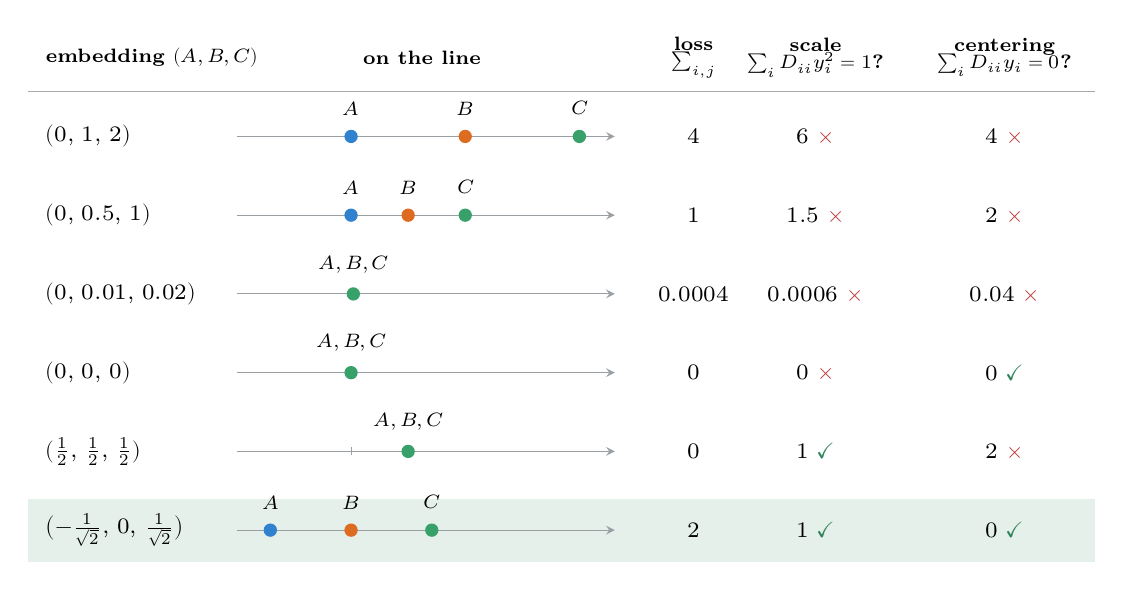
\begin{tikzpicture}[>=stealth, x=1cm, y=1cm,
  A/.style={circle, fill=dataC, inner sep=1.7pt},
  B/.style={circle, fill=accentC, inner sep=1.7pt},
  C/.style={circle, fill=accentD, inner sep=1.7pt},
  lab/.style={font=\scriptsize, above=1.5pt}]
\newcommand{\yes}{\textcolor{intgreen}{$\checkmark$}}
\newcommand{\no}{\textcolor{thmred}{$\times$}}
\def\xs{1.45}
\newcommand{\rowline}[6]{%
  \node[font=\footnotesize, anchor=west] at (-0.3,#1) {#2};
  \draw[->, ink!45] (2.25,#1) -- (7.05,#1);
  \draw[ink!45] ({3.7+0*\xs},{#1-0.05}) -- ({3.7+0*\xs},{#1+0.05});
  \node[font=\footnotesize] at (8.05,#1) {#3};
  \node[font=\footnotesize] at (9.6,#1) {#4};
  \node[font=\footnotesize] at (12.0,#1) {#5};
  #6}
\fill[intgreen!12] (-0.4,-5.85) rectangle (13.15,-5.05);
\node[font=\scriptsize\bfseries, anchor=west] at (-0.3,0.55) {embedding $(A,B,C)$};
\node[font=\scriptsize\bfseries] at (4.6,0.55) {on the line};
\node[font=\scriptsize\bfseries, align=center] at (8.05,0.55) {loss\\[-2pt]$\sum_{i,j}$};
\node[font=\scriptsize\bfseries, align=center] at (9.6,0.55) {scale\\[-2pt]$\sum_iD_{ii}y_i^2=1$?};
\node[font=\scriptsize\bfseries, align=center] at (12.0,0.55) {centering\\[-2pt]$\sum_iD_{ii}y_i=0$?};
\draw[ink!40] (-0.4,0.12) -- (13.15,0.12);
\rowline{-0.45}{$(0,\,1,\,2)$}{$4$}{$6$ \no}{$4$ \no}
  {\node[A,label={[lab]$A$}] at ({3.7+0*\xs},-0.45) {};\node[B,label={[lab]$B$}] at ({3.7+1*\xs},-0.45) {};\node[C,label={[lab]$C$}] at ({3.7+2*\xs},-0.45) {};}
\rowline{-1.45}{$(0,\,0.5,\,1)$}{$1$}{$1.5$ \no}{$2$ \no}
  {\node[A,label={[lab]$A$}] at ({3.7+0*\xs},-1.45) {};\node[B,label={[lab]$B$}] at ({3.7+0.5*\xs},-1.45) {};\node[C,label={[lab]$C$}] at ({3.7+1*\xs},-1.45) {};}
\rowline{-2.45}{$(0,\,0.01,\,0.02)$}{$0.0004$}{$0.0006$ \no}{$0.04$ \no}
  {\node[C,label={[lab]$A,B,C$}] at ({3.7+0.02*\xs},-2.45) {};}
\rowline{-3.45}{$(0,\,0,\,0)$}{$0$}{$0$ \no}{$0$ \yes}
  {\node[C,label={[lab]$A,B,C$}] at ({3.7+0*\xs},-3.45) {};}
\rowline{-4.45}{$(\tfrac12,\,\tfrac12,\,\tfrac12)$}{$0$}{$1$ \yes}{$2$ \no}
  {\node[C,label={[lab]$A,B,C$}] at ({3.7+0.5*\xs},-4.45) {};}
\rowline{-5.45}{$\big({-}\tfrac1{\sqrt2},\,0,\,\tfrac1{\sqrt2}\big)$}{$2$}{$1$ \yes}{$0$ \yes}
  {\node[A,label={[lab]$A$}] at ({3.7-0.7071*\xs},-5.45) {};\node[B,label={[lab]$B$}] at ({3.7+0*\xs},-5.45) {};\node[C,label={[lab]$C$}] at ({3.7+0.7071*\xs},-5.45) {};}
\end{tikzpicture}
\caption{The loss falls as the picture shrinks and reaches $0$ when all three points coincide. The last row is the only one that passes both constraints. Its loss is higher than that of the shrunken and collapsed rows, but those rows are not allowed. It is also the first row with its position and size corrected: subtract the weighted mean $1$ from $(0,1,2)$ and divide by $\sqrt2$. The loss column is the full double sum, which is $2\tr(Y\T LY)$, so the last row has $\tr(Y\T LY)=1=\lambda_2$ as in Example~\ref{ex:lepath} (with the sign of the coordinate flipped).}
\label{fig:pullonly}
\end{figure}

Without constraints the objective has three blind spots:
\begin{enumerate}[nosep,label=(\alph*)]
\item \textbf{Collapse.} $Y=0_{N\times t}$ puts every point at the origin and scores $0$, which is unbeatable. The scaling constraint forbids it,
because $Y\T DY=I_t$ is impossible for $Y=0$. This is not only about the exact point $Y=0$: any embedding improves by shrinking, since
$\tr\big((cY)\T L(cY)\big)=c^2\tr(Y\T LY)$ is smaller for every $0<c<1$. Without a fixed scale, the objective always prefers a smaller picture.
\item \textbf{Translation.} Moving every point by the same $\bm c$ leaves every $\bm y_i-\bm y_j$ unchanged, so the objective cannot say where
the cloud sits. Worse, a column of $Y$ that is constant (all points at the same coordinate) costs $0$, since $L\one=\bm0$. Scaling alone would
pick that column, a whole dimension that says nothing about the data. The centering constraint rules it out.
\item \textbf{Rotation.} If $Y$ is optimal, so is $YQ$ for any orthogonal $Q\in\R^{t\times t}$, because $\tr(Q\T Y\T LYQ)=\tr(Y\T LY)$ and
$Q\T Y\T DYQ=I$. The answer is unique only up to rotation and reflection, the same sign ambiguity as PCA loadings. No constraint fixes this,
and none is needed.
\end{enumerate}

\begin{figure}[htbp]
\centering
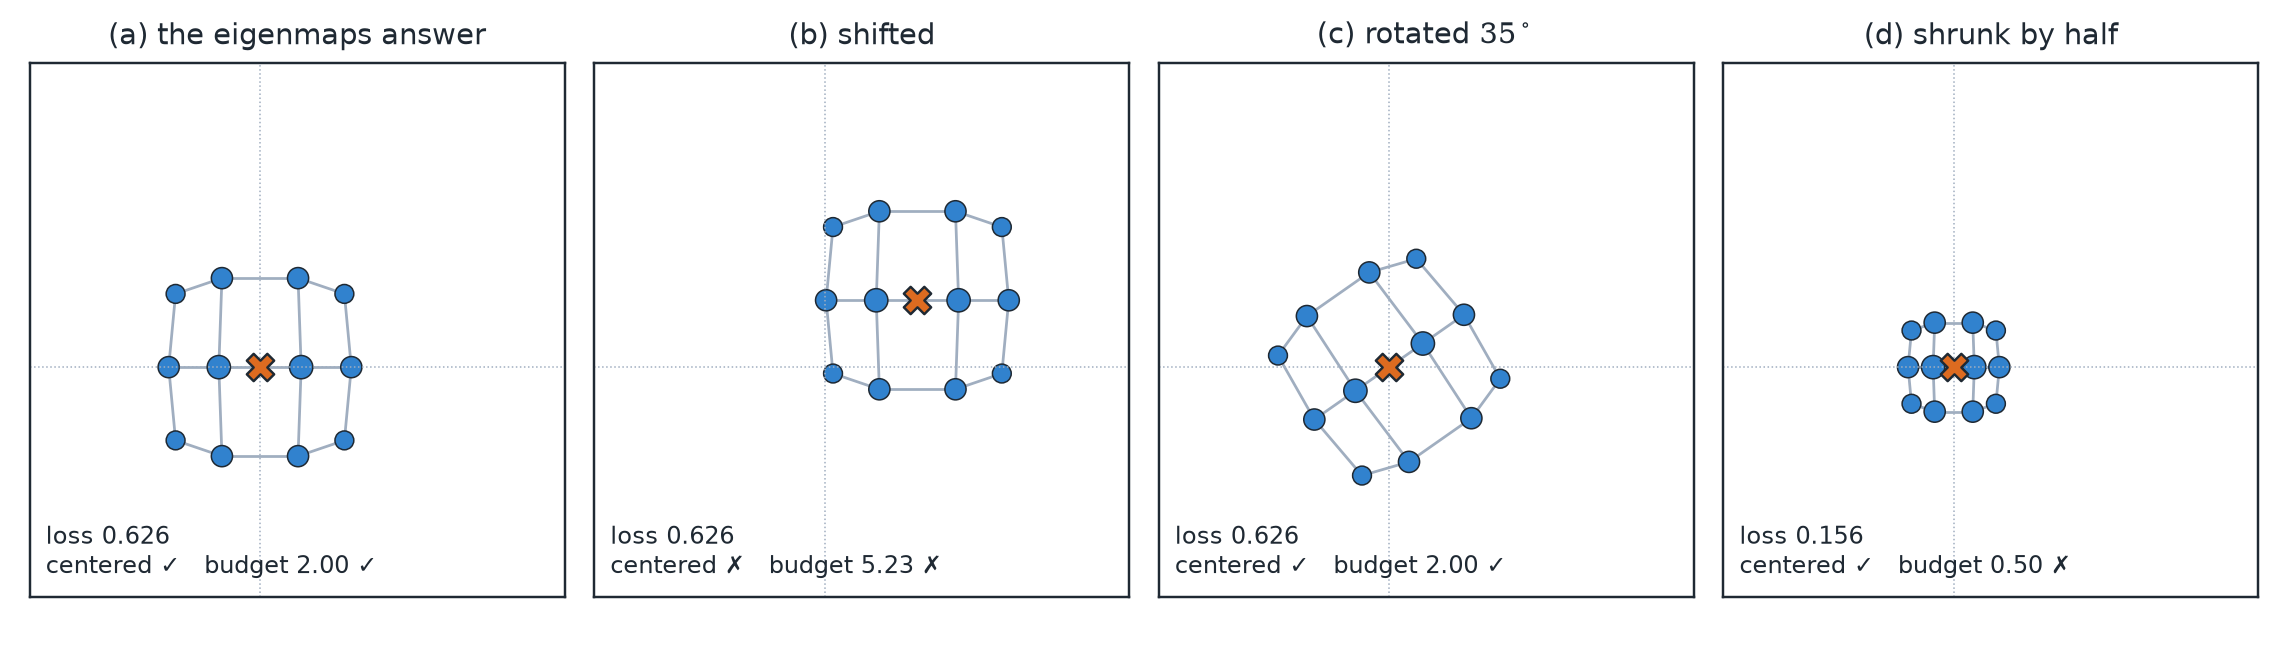
\includegraphics[width=\textwidth]{figures/le_blindspots.png}
\caption{The three blind spots on a $3\times4$ grid graph, $t=2$. Point size grows with degree, the orange cross is the degree-weighted centroid $\sum_iD_{ii}\bm y_i/\sum_iD_{ii}$, and the budget is $\sum_iD_{ii}\norm{\bm y_i}^2$, which must equal $t=2$. \emph{(a)} The eigenmaps answer, with loss $0.626$. \emph{(b)} Shifting changes no edge length, so the loss is still $0.626$, but the centroid leaves the origin (and the budget jumps to $5.23$), so the constraints reject it. \emph{(c)} Rotating also keeps the loss at $0.626$, and both constraints still hold: this is the freedom that remains, and it costs nothing. \emph{(d)} Halving every coordinate quarters the loss, to $0.156$, which is why the unconstrained optimum shrinks to a point. The budget ($0.50\ne2$) rejects it.}
\label{fig:leblind}
\end{figure}

\textbf{Translation is harmless alone, but essential once scale is fixed.} By itself, translation is only an ambiguity: many answers that are all the same picture. Once scale is fixed, though, it becomes a way to cheat. Take a constant embedding such as $(5,5,5)$ and resize it to $(\tfrac12,\tfrac12,\tfrac12)$, so that $\sum_iD_{ii}y_i^2=\tfrac14+\tfrac24+\tfrac14=1$. It passes the scale constraint with a loss of $0$, because the points are all together, just away from the origin. Scale alone therefore does not stop the collapse. Centering closes the gap: if every $\bm y_i=\bm c$, then $\sum_iD_{ii}\bm y_i=\big(\sum_iD_{ii}\big)\bm c=\bm 0$ forces $\bm c=\bm0$, which has size zero and fails the scale constraint. In the eigenvector solution, this cheat is $D^{-1/2}\vv_1\propto\one_N$, which is why $\vv_1$ is thrown away.

\begin{center}
\renewcommand{\arraystretch}{1.3}
\small
\begin{tabular}{>{\raggedright\arraybackslash}p{5.3cm}>{\raggedright\arraybackslash}p{4.6cm}>{\raggedright\arraybackslash}p{4.1cm}}
\toprule
Way of crushing the picture & Example on the chain & Blocked by\\
\midrule
Shrink toward zero & $(0,0.01,0.02)$, $(0,0,0)$ & fixed scale (diagonal of $Y\T DY=I_t$)\\
All points at one location & $(\tfrac12,\tfrac12,\tfrac12)$ & centering together with fixed scale\\
A $t$-dimensional picture that is secretly lower-dimensional & $(\bm y,\bm y)$: same column twice, a diagonal line & orthogonal coordinates (off-diagonal of $Y\T DY=I_t$)\\
\bottomrule
\end{tabular}
\end{center}

\begin{careful}
\textbf{The constraints are mostly, but not entirely, free.} Position and overall size were never things we cared about, so pinning them down costs nothing. On the chain, the constrained answer is exactly the sensible shape $(0,1,2)$ moved and resized. Two effects do go beyond position and overall size.
\textbf{Each axis gets its own fixed spread.} $Y\T DY=I_t$ gives every coordinate the same weighted spread, so the plot's aspect ratio carries no information: a long thin manifold does not come out long and thin.
\textbf{The spread is weighted by degree,} which is what pushes low-degree points outward (see below).
Also, ruling out ``all points identical'' does not rule out ``nearly identical within groups.'' With nearly separate clusters, each cluster still bunches up, as in Figure~\ref{fig:clusters}.
\end{careful}

\textbf{Reading the constraints entrywise.} Since $D$ is diagonal, $D\one_N=(D_{11},\dots,D_{NN})\T$, so
\[
Y\T D\one_N=\sum_{i=1}^ND_{ii}\,\bm y_i=\bm0
\qquad\text{and}\qquad
Y\T DY=\sum_{i=1}^ND_{ii}\,\bm y_i\bm y_i\T=I_t\ \ \Longrightarrow\ \ \sum_{i=1}^ND_{ii}\norm{\bm y_i}^2=\tr(I_t)=t .
\]
The first is \textbf{degree-weighted centering}: the weighted centroid sits at the origin, and high-degree points count more. Compare
$\xbar=\bm 0$ in PCA, which is the same statement with every weight equal to $1$. The second is a fixed \textbf{budget}: the squared
distances from the origin, weighted by degree, add up to exactly $t$. In matrix form, $D^{1/2}Y$ has rows $\sqrt{D_{ii}}\,\bm y_i\T$, so
$Y\T DY=(D^{1/2}Y)\T(D^{1/2}Y)$: the scaling constraint says the columns of $D^{1/2}Y$ are orthonormal.

\textbf{What $\bm y\T D\one=0$ really says: orthogonal to constants, in a weighted dot product.} Take one coordinate $\bm y$ and define the weighted dot product $\langle\bm x,\bm y\rangle_D=\bm x\T D\bm y=\sum_iD_{ii}x_iy_i$. Then centering is $\langle\bm y,\one\rangle_D=0$. Dividing by the total degree shows the same thing as a weighted average:
\[
\frac{\sum_iD_{ii}y_i}{\sum_iD_{ii}}=0 ,
\]
so the positions balance around zero, with highly connected vertices counting more. A constant vector $\bm y=c\one$ gives $c\,\one\T D\one=c\sum_iD_{ii}$, which is zero only for $c=0$ (any graph with an edge has $\sum_iD_{ii}>0$). And the scale constraint alone allows one nonzero constant in general, $\bm y=\one/\sqrt{\one\T D\one}$. On the chain this is $\one/\sqrt4=(\tfrac12,\tfrac12,\tfrac12)$, the cheat in Figure~\ref{fig:pullonly}.

The weights matter. On the chain, $(-3,1,1)$ is allowed because $-3+2\cdot1+1=0$, even though its ordinary dot product with $\one$ is $-1$. Likewise, a guess like $(-1,-1,0,1,1)$ on five vertices is allowed only if $D_{11}+D_{22}=D_{44}+D_{55}$. On the graph of Example~\ref{ex:rwfive} it is not: $-1-1+\tfrac34+\tfrac34=-\tfrac12$.

\begin{example}{No constant pattern survives both constraints}{noconstant}
Take three vertices with degrees $d_1,d_2,d_3$ (not all zero) and place every vertex at the same coordinate, $\bm y=(c,c,c)\T$. Do the multiplication one piece at a time. First $D\one$ collects the degrees, and then $\bm y\T$ multiplies them by $c$:
\[
D\one=\begin{bmatrix}d_1&0&0\\0&d_2&0\\0&0&d_3\end{bmatrix}\begin{bmatrix}1\\1\\1\end{bmatrix}=\begin{bmatrix}d_1\\d_2\\d_3\end{bmatrix},
\qquad
\bm y\T D\one=\begin{bmatrix}c&c&c\end{bmatrix}\begin{bmatrix}d_1\\d_2\\d_3\end{bmatrix}=c\,(d_1+d_2+d_3).
\]
The same steps give the scale constraint, $\bm y\T D\bm y=c^2(d_1+d_2+d_3)$. Each constraint now pins down $c$, and they disagree:
\[
\underbrace{c\,(d_1+d_2+d_3)=0}_{\text{centering}}\ \Longrightarrow\ c=0,
\qquad\qquad
\underbrace{c^2(d_1+d_2+d_3)=1}_{\text{scale}}\ \Longrightarrow\ c=\pm\frac1{\sqrt{d_1+d_2+d_3}}.
\]
Since $d_1+d_2+d_3>0$, no value of $c$ does both. Here it is on the chain, with degrees $(1,2,1)$, so $\bm y\T D\one=4c$ and $\bm y\T D\bm y=4c^2$:
\begin{center}
\small
\renewcommand{\arraystretch}{1.2}
\begin{tabular}{@{}lrcrc@{}}
\toprule
$\bm y$ & $\bm y\T D\one$ & equals $0$? & $\bm y\T D\bm y$ & equals $1$? \\
\midrule
$(1,1,1)$ & $4$ & \textcolor{thmred}{$\times$} & $4$ & \textcolor{thmred}{$\times$} \\
$(5,5,5)$ & $20$ & \textcolor{thmred}{$\times$} & $100$ & \textcolor{thmred}{$\times$} \\
$(-2,-2,-2)$ & $-8$ & \textcolor{thmred}{$\times$} & $16$ & \textcolor{thmred}{$\times$} \\
$(\tfrac12,\tfrac12,\tfrac12)$ & $2$ & \textcolor{thmred}{$\times$} & $1$ & \textcolor{intgreen}{$\checkmark$} \\
$(-\tfrac12,-\tfrac12,-\tfrac12)$ & $-2$ & \textcolor{thmred}{$\times$} & $1$ & \textcolor{intgreen}{$\checkmark$} \\
$(0,0,0)$ & $0$ & \textcolor{intgreen}{$\checkmark$} & $0$ & \textcolor{thmred}{$\times$} \\
\bottomrule
\end{tabular}
\end{center}
On the number line of possible values of $c$, the two constraints mark different points:
\begin{center}
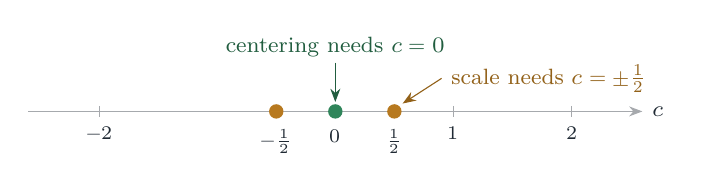
\begin{tikzpicture}[x=1.5cm, y=1cm]
\draw[-{Stealth}, softgray!70!black] (-2.6,0) -- (2.6,0) node[right, font=\footnotesize, ink] {$c$};
\foreach \c/\l in {-2/-2,1/1,2/2} {
  \draw[softgray!70!black] (\c,0.07) -- (\c,-0.07);
  \node[font=\scriptsize, below=2pt, ink] at (\c,0) {$\l$};
}
\fill[intgreen] (0,0) circle (2.6pt);
\node[font=\scriptsize, below=3pt, ink] at (0,0) {$0$};
\fill[warnamber] (-0.5,0) circle (2.6pt);
\fill[warnamber] (0.5,0) circle (2.6pt);
\node[font=\scriptsize, below=3pt, ink] at (-0.5,0) {$-\tfrac12$};
\node[font=\scriptsize, below=3pt, ink] at (0.5,0) {$\tfrac12$};
\node[font=\footnotesize, intgreen!70!black] at (0,0.82) {centering needs $c=0$};
\draw[intgreen!70!black, -{Stealth}] (0,0.62) -- (0,0.12);
\node[font=\footnotesize, warnamber!80!black, anchor=west] at (0.9,0.42) {scale needs $c=\pm\tfrac12$};
\draw[warnamber!80!black, -{Stealth}] (0.9,0.42) -- (0.57,0.1);
\end{tikzpicture}
\end{center}
This only rules out one value shared by \emph{every} vertex. If the graph is disconnected, a coordinate that is constant on each piece can pass both constraints with loss $0$. For two separate edges, all degrees are $1$, and $(\tfrac12,\tfrac12,-\tfrac12,-\tfrac12)$ has $\bm y\T D\one=0$, $\bm y\T D\bm y=1$, and no edge crossing the split. That is the repeated $\lambda=0$ behind spectral clustering.
\end{example}

\textbf{Centering blocks partly constant embeddings too.} Split any $\bm y$ into a constant part and a centered part:
\[
\bm y=c\one+\bm z,\qquad c=\frac{\bm y\T D\one}{\one\T D\one}\ \ (\text{the weighted mean}),\qquad \bm z\T D\one=0 .
\]
The cross term vanishes because $\bm z\T D\one=0$, and $L\one=\bm0$ removes the constant from the loss:
\[
\bm y\T D\bm y=\underbrace{c^2\,\one\T D\one}_{\text{budget wasted on the constant}}+\underbrace{\bm z\T D\bm z}_{\text{budget left for shape}},
\qquad
\bm y\T L\bm y=\bm z\T L\bm z .
\]
So the constant part spends the budget and contributes nothing to the loss. That is a discount: the more budget goes to the constant, the smaller $\bm z$ has to be and the lower the loss. Centering sets $c=0$, so the whole budget goes to the shape. Take $(0,1,2)$ on the chain: $c=1$ and $\bm z=(-1,0,1)$, with budget $6=4+2$. Rescaled to meet the scale constraint, $(0,1,2)/\sqrt6$ has loss $\tfrac13$, which beats the true optimum $\lambda_2=1$ only because it is not centered.

\begin{figure}[htbp]
\centering
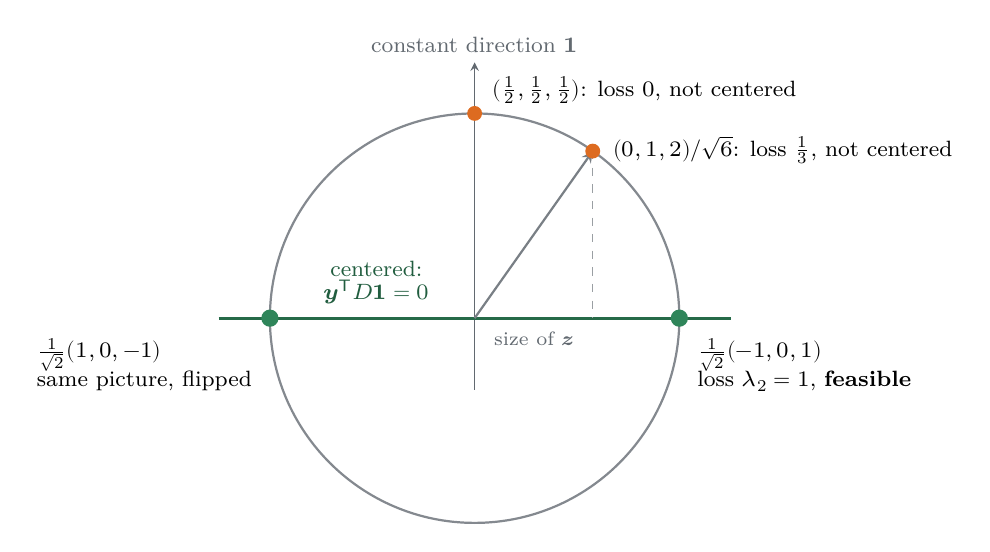
\begin{tikzpicture}[>=stealth, x=2.6cm, y=2.6cm,
  pt/.style={circle, fill=accentC, inner sep=1.9pt},
  good/.style={circle, fill=intgreen, inner sep=2.2pt},
  lab/.style={font=\footnotesize, align=left}]
\draw[ink!55, thick] (0,0) circle (1);
\draw[->, ink!70] (0,-0.35) -- (0,1.25) node[above, font=\footnotesize, align=center] {constant direction $\one$};
\draw[intgreen!80!black, very thick] (-1.25,0) -- (1.25,0);
\node[font=\footnotesize, intgreen!70!black, anchor=south, align=center] at (-0.48,0.02) {centered:\\[-1pt]$\bm y\T D\one=0$};
\draw[dashed, ink!45] (0.577,0.816) -- (0.577,0);
\draw[ink!60, thick, ->] (0,0) -- (0.577,0.816);
\node[pt] at (0,1) {};
\node[lab, anchor=south west] at (0.04,1.0) {$(\tfrac12,\tfrac12,\tfrac12)$: loss $0$, not centered};
\node[pt] at (0.577,0.816) {};
\node[lab, anchor=west] at (0.63,0.82) {$(0,1,2)/\sqrt6$: loss $\tfrac13$, not centered};
\node[good] at (1,0) {};
\node[lab, anchor=north west] at (1.04,-0.05) {$\tfrac1{\sqrt2}(-1,0,1)$\\[-1pt]loss $\lambda_2=1$, \textbf{feasible}};
\node[good] at (-1,0) {};
\node[lab, anchor=north east] at (-1.04,-0.05) {$\tfrac1{\sqrt2}(1,0,-1)$\\[-1pt]same picture, flipped};
\node[font=\scriptsize, ink!70, anchor=north] at (0.29,-0.02) {size of $\bm z$};
\end{tikzpicture}
\caption{All vectors with $\bm y\T D\bm y=1$ on the chain form a sphere; this is the slice through $\one$ and the optimal direction, with lengths and angles measured in the weighted dot product. Height is the constant part and horizontal position is the centered part $\bm z$. On this slice, the loss $\bm y\T L\bm y$ is $\lambda_2$ times the squared horizontal position, so it falls as you climb toward the constant vector. Centering leaves only the two points where the circle meets the horizontal line, and they are mirror images. For the full problem, centering also allows the direction of $\vv_3$, which is out of the page and has higher loss.}
\label{fig:dorth}
\end{figure}

\textbf{Which ``first eigenvector'' is being skipped.} $\one$ is an eigenvector of $L$ with eigenvalue $0$, since $(L\one)_i=D_{ii}-\sum_jA_{ij}=0$. But the embedding does not use the eigenvectors of $L$ itself. It uses the generalized problem $L\vu=\lambda D\vu$, whose first solution is also $\one$, and whose second is the second-smallest $\lambda$ of $L_{\mathrm{sym}}$ and $L_{\mathrm{rw}}$. On the chain these differ: $L$ has eigenvalues $\{0,1,3\}$ and the generalized problem has $\{0,1,2\}$ (Example~\ref{ex:lepath}). Also, $\one$ is the unique such solution only on a connected graph. With several components, $\lambda=0$ repeats and the next coordinates are constant on each component.

\textbf{The off-diagonal entries do a second job.} The budget above only uses the trace of $Y\T DY=I_t$. Writing $\bm y^{(j)}$ for column $j$ of $Y$ (coordinate $j$ of every point), the full matrix equation says
\[
\sum_{i=1}^ND_{ii}\,y^{(j)}_i\,y^{(k)}_i=\begin{cases}1 & j=k\quad(\text{each coordinate has the same weighted spread}),\\ 0 & j\ne k\quad(\text{different coordinates are degree-weighted orthogonal}).\end{cases}
\]
The second line stops all $t$ coordinates from secretly being the same one-dimensional direction. Figure~\ref{fig:capacity} shows what goes wrong without it.

\begin{intuition}
\textbf{Who ends up near the origin?} Under the budget $\sum_iD_{ii}\norm{\bm y_i}^2=t$, a high-degree point pays more for each unit of squared distance from the origin, and a
low-degree point pays less. So low-degree points are ``free'' to take large coordinates, and high-degree points tend to sit nearer the origin.
On a sampled manifold, interior points have many neighbors and boundary points have fewer, so the boundary gets pushed outward.
This is a tendency, not a law: the objective still decides where each point goes.
\textbf{Which constraint does it.} Your notes credit the centering constraint for putting high-degree nodes near the origin. Centering only
says the $D$-weighted mean is $\bm 0$. The pull toward the origin comes mostly from the scaling budget, and the explicit formula below makes it
concrete: $\bm y_i$ equals a unit-scale eigenvector entry divided by $\sqrt{D_{ii}}$.
\end{intuition}

\subsubsection*{Step 4: solving it. The generalized eigenproblem and three Laplacians}

\textbf{Lagrange conditions.} Take $\mathcal L(Y,\Lambda)=\tr(Y\T LY)-\tr\big(\Lambda(Y\T DY-I_t)\big)$ with a symmetric multiplier
$\Lambda$. Setting the gradient to zero gives $2LY-2DY\Lambda=0$, so $LY=DY\Lambda$. Rotating $Y$ (blind spot (c)) diagonalizes $\Lambda$, and
then each column $\vu$ of $Y$ satisfies
\[
L\vu=\lambda D\vu\qquad(\text{a \textbf{generalized} eigenproblem: } D \text{ appears on the right}).
\]

\textbf{Where the $2$ in $2LY$ comes from.} The step ``setting the gradient to zero'' uses one fact about quadratic forms. It is stated here with a general matrix $M$, because $A$ already means the adjacency matrix.

\begin{proposition}{Gradient of a quadratic form}{gradquad}
For any $n\times n$ matrix $M$ and $\bm y\in\R^n$,
\[
\nabla_{\bm y}\big(\bm y\T M\bm y\big)=(M+M\T)\bm y,\qquad\text{which is } 2M\bm y \text{ when } M=M\T .
\]
This is a statement about the \emph{gradient}. The quadratic form $\bm y\T M\bm y$ itself is a single number.
\end{proposition}
\begin{proofsketch}
Write the number with indices, $\bm y\T M\bm y=\sum_{i=1}^n\sum_{j=1}^ny_iM_{ij}y_j$, and differentiate the whole double sum with respect to one coordinate $y_k$. A term $y_iM_{ij}y_j$ can contain $y_k$ in two places, so the product rule gives two pieces:
\[
\frac{\partial}{\partial y_k}\big(y_iM_{ij}y_j\big)=\underbrace{\frac{\partial y_i}{\partial y_k}M_{ij}y_j}_{y_i\text{ might be }y_k}+\underbrace{y_iM_{ij}\frac{\partial y_j}{\partial y_k}}_{y_j\text{ might be }y_k},
\qquad
\frac{\partial y_i}{\partial y_k}=\delta_{ik}=\begin{cases}1&i=k,\\0&i\ne k.\end{cases}
\]
Summing over $i$ and $j$, each $\delta$ keeps only the terms where its index equals $k$:
\[
\frac{\partial}{\partial y_k}\big(\bm y\T M\bm y\big)=\sum_{i,j}\big(\delta_{ik}M_{ij}y_j+y_iM_{ij}\delta_{jk}\big)
=\underbrace{\sum_jM_{kj}y_j}_{i=k:\ (M\bm y)_k}+\underbrace{\sum_iM_{ik}y_i}_{j=k:\ (M\T\bm y)_k}.
\]
Stacking these partial derivatives for $k=1,\dots,n$ gives $M\bm y+M\T\bm y=(M+M\T)\bm y$.
\end{proofsketch}

\textbf{Reading $(M\T\bm y)_k$: one free index, one summed index.} The subscript $k$ in $(M\T\bm y)_k$ says which entry of the output vector you want. It is fixed, not summed. By the definition of a matrix times a vector, entry $k$ is row $k$ of the matrix dotted with $\bm y$:
\[
(B\bm y)_k=\sum_{i=1}^nB_{ki}\,y_i\qquad(k\text{ picks the row and stays fixed; }i\text{ runs along that row}).
\]
Take $B=M\T$. Transposing swaps the two labels, $(M\T)_{ki}=M_{ik}$, so
\[
(M\T\bm y)_k=\sum_{i=1}^nM_{ik}\,y_i ,
\]
which is exactly the second sum in the proof. For example, $(M\T\bm y)_2=M_{12}y_1+M_{22}y_2+\cdots+M_{n2}y_n$ runs down \emph{column} $2$ of $M$, which is row $2$ of $M\T$.

\begin{careful}
\begin{itemize}[nosep,leftmargin=*]
\item \textbf{One line, not two sums.} You can differentiate $\sum_{i,j}y_iM_{ij}y_j$ in one step with the product rule; you do not have to split the sum first. The two pieces appear because $\bm y$ appears twice in the expression, once on the left and once on the right. The split only makes the two contributions visible.
\item \textbf{The usual slip is to count $\bm y$ once.} Doing so gives $M\bm y$, which is half the answer for symmetric $M$ and the wrong vector otherwise. Check with $M=\begin{bmatrix}1&2\\0&3\end{bmatrix}$: $\bm y\T M\bm y=y_1^2+2y_1y_2+3y_2^2$ has gradient $(2y_1+2y_2,\ 2y_1+6y_2)\T=(M+M\T)\bm y$, while $M\bm y=(y_1+2y_2,\ 3y_2)\T$.
\end{itemize}
\end{careful}

\textbf{Back to the Lagrangian.} $\tr(Y\T LY)=\sum_j\bm y^{(j)\top}L\,\bm y^{(j)}$ is a sum of quadratic forms, one per column $\bm y^{(j)}$ of $Y$, and $L=L\T$. So by Proposition~\ref{prop:gradquad} its gradient with respect to column $j$ is $2L\bm y^{(j)}$, and stacking the columns gives $2LY$. The same computation for the constraint term, with the symmetric $\Lambda$ mixing the columns, gives $2DY\Lambda$. The $2$s cancel, leaving $LY=DY\Lambda$.

\begin{careful}
\textbf{$\vu\T D\vu=1$ is not the same as $\vu\T L\vu=1$.} The two quadratic forms measure different things:
\begin{align*}
\vu\T D\vu&=\textstyle\sum_iD_{ii}u_i^2 && (\text{weighted \emph{size}: fixed at }1),\\
\vu\T L\vu&=\tfrac12\textstyle\sum_{i,j}A_{ij}(u_i-u_j)^2 && (\text{\emph{roughness}: made as small as possible}).
\end{align*}
The problem is $\min\vu\T L\vu$ subject to $\vu\T D\vu=1$ (no shrinking to zero) and $\vu\T D\one=0$ (no constant vector). Fixing the roughness at $1$ would make no sense, since the roughness is the thing being minimized. The two forms are linked only at a solution: multiplying $L\vu=\lambda D\vu$ on the left by $\vu\T$ gives
\[
\vu\T L\vu=\lambda\,\vu\T D\vu=\lambda .
\]
So each eigenvalue is the roughness of its own $D$-normalized eigenvector. It equals $1$ only when that eigenvalue happens to be $1$. On the chain, the generalized eigenvalues are $\{0,1,2\}$. $\vu_2=(\tfrac1{\sqrt2},0,-\tfrac1{\sqrt2})$ has size $\tfrac12+0+\tfrac12=1$ and roughness $\tfrac12+\tfrac12=1$, a coincidence of this graph. $\vu_3=(\tfrac12,-\tfrac12,\tfrac12)$ also has size $\tfrac14+\tfrac24+\tfrac14=1$, but its roughness is $1+1=2$.
\end{careful}

\textbf{Route 1: multiply by $D^{-1}$.} Assume $D$ is invertible, i.e.\ every degree is positive (no isolated vertex; a $k$-NN graph guarantees this,
an $\varepsilon$-ball graph may not, see Figure~\ref{fig:epsknn}). Then
\[
D^{-1}L\vu=(I-D^{-1}A)\vu=\lambda\vu .
\]
$L_{\mathrm{rw}}=I-D^{-1}A$ is the \textbf{random-walk Laplacian}. The name comes from $P=D^{-1}A$, which has entries $P_{ij}=A_{ij}/D_{ii}$ and rows summing to
$1$: it is the transition matrix of a random walk that steps from $i$ to a neighbor $j$ with probability proportional to $A_{ij}$. The catch is
that $L_{\mathrm{rw}}$ is \textbf{not symmetric} (row $i$ is divided by $D_{ii}$, column $i$ is not), so the spectral theorem does not apply directly. Example~\ref{ex:rwfive} below works through what $L_{\mathrm{rw}}$ does on a small graph.

\textbf{Route 2: change variables to get a symmetric problem.} Let $D^{1/2}=\diag(\sqrt{D_{11}},\dots,\sqrt{D_{NN}})$ and set
\[
\widetilde Y=D^{1/2}Y\qquad\big(\text{so } Y=D^{-1/2}\widetilde Y\big).
\]
Each piece of the problem translates:
\begin{align*}
\text{scaling:}\quad & Y\T DY=Y\T D^{1/2}D^{1/2}Y=\widetilde Y\T\widetilde Y=I_t,\\
\text{centering:}\quad & Y\T D\one_N=Y\T D^{1/2}\,D^{1/2}\one_N=\widetilde Y\T\big(D^{1/2}\one_N\big)=\bm0,\\
\text{objective:}\quad & \tr(Y\T LY)=\tr\big(\widetilde Y\T D^{-1/2}LD^{-1/2}\,\widetilde Y\big)=\tr\big(\widetilde Y\T L_{\mathrm{sym}}\widetilde Y\big),
\end{align*}
where
\[
L_{\mathrm{sym}}=D^{-1/2}LD^{-1/2}=D^{-1/2}(D-A)D^{-1/2}=I-D^{-1/2}AD^{-1/2},\qquad (L_{\mathrm{sym}})_{ij}=-\frac{A_{ij}}{\sqrt{D_{ii}D_{jj}}}\ \ (i\ne j),
\]
is the \textbf{symmetric normalized graph Laplacian}. The new problem is
\[
\min_{\widetilde Y\in\R^{N\times t}}\ \tr\big(\widetilde Y\T L_{\mathrm{sym}}\widetilde Y\big)\quad\text{s.t.}\quad \widetilde Y\T\widetilde Y=I_t,\ \ \widetilde Y\T D^{1/2}\one_N=\bm0 .
\]
Solve for $\widetilde Y$, then take $Y=D^{-1/2}\widetilde Y$.

\textbf{The picture behind both routes.} Look at one coordinate $\bm y$ and only two of its entries, so everything can be drawn in the plane (Figure~\ref{fig:letangency}). The level curves of the loss $\bm y\T L\bm y$ are nested ellipses, and the constraint $\bm y\T D\bm y=1$ is one more ellipse. Slide along the constraint: the loss is smallest where a level curve just \emph{touches} the constraint without crossing it. At a touching point the two curves share a tangent line, so their normal directions agree, and the normals are the gradients:
\[
\nabla(\bm y\T L\bm y)=2L\bm y\ \ \parallel\ \ \nabla(\bm y\T D\bm y)=2D\bm y
\qquad\Longleftrightarrow\qquad L\bm y=\lambda D\bm y .
\]
That is the Lagrange condition, read off a picture. Multiplying by $\bm y\T$ gives $\bm y\T L\bm y=\lambda\,\bm y\T D\bm y=\lambda$, so the loss at a touching point \emph{is} its $\lambda$. The other touching point, where the largest level curve touches from outside, is the other generalized eigenvector. In the original coordinates the two solutions are not perpendicular; they are perpendicular only in the $D$-weighted sense, $\vu_1\T D\vu_2=0$. Route 2's substitution $\widetilde{\bm y}=D^{1/2}\bm y$ stretches axis $i$ by $\sqrt{D_{ii}}$. That turns the constraint ellipse into the unit circle, the problem into an ordinary eigenproblem for the symmetric $L_{\mathrm{sym}}$, and the $D$-orthogonal solutions into ordinary perpendicular eigenvectors.

\begin{figure}[htbp]
\centering
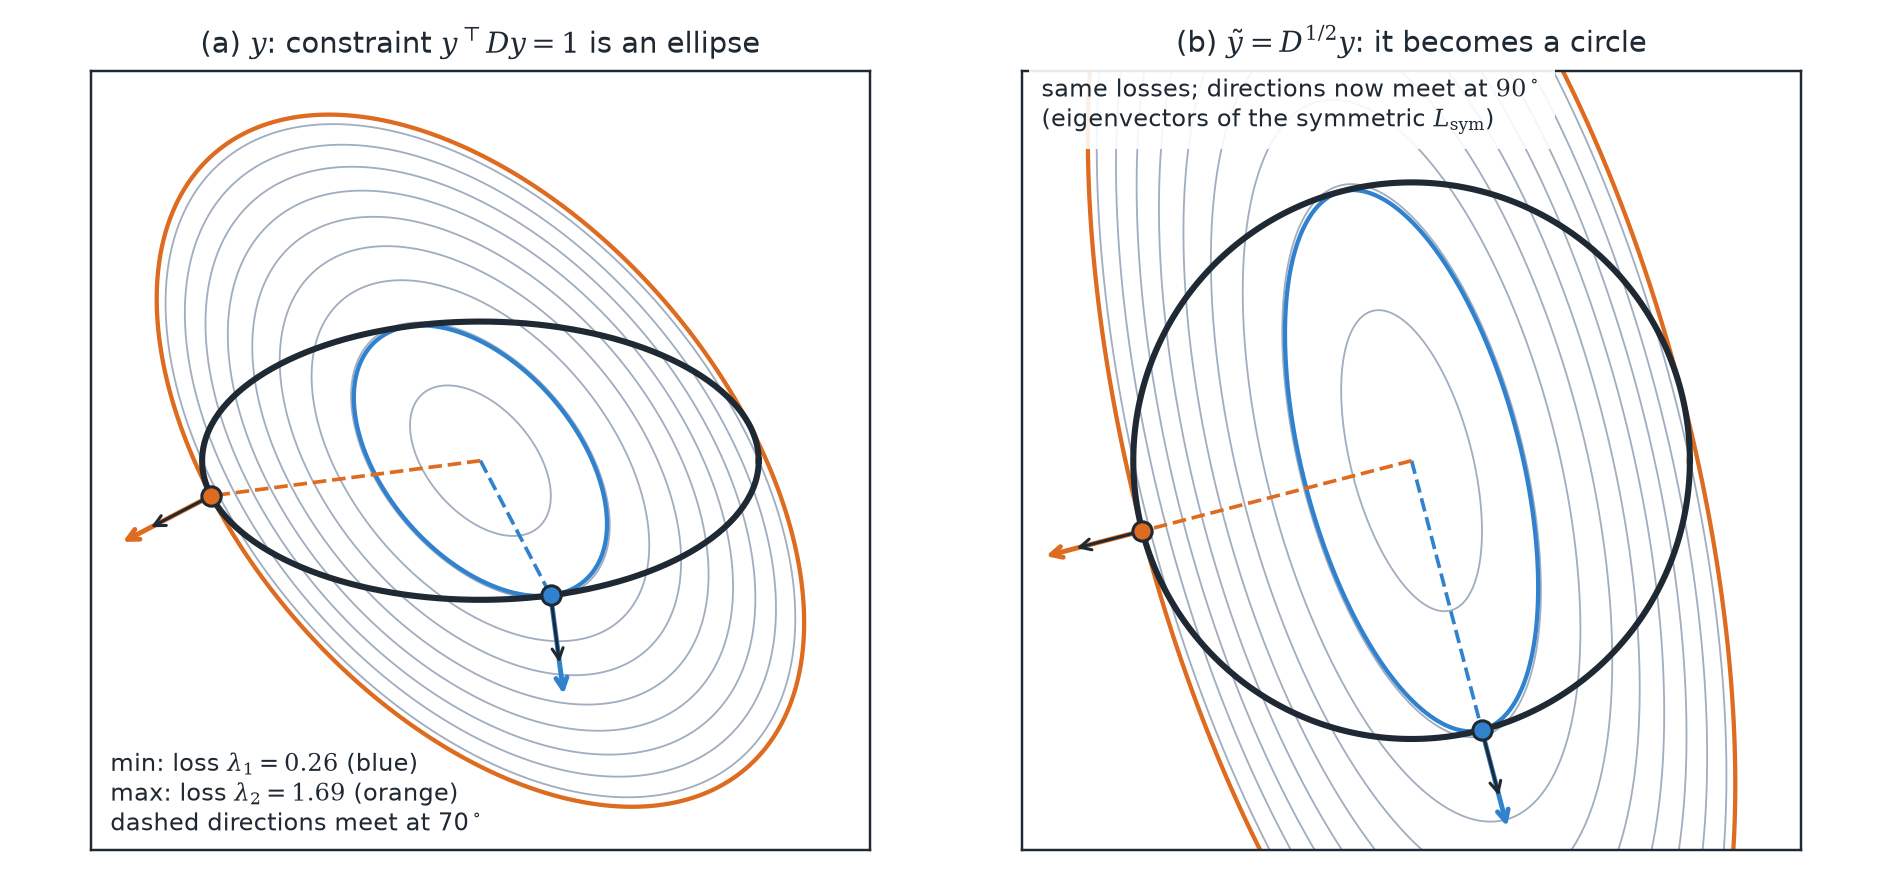
\includegraphics[width=0.92\textwidth]{figures/le_tangency.png}
\caption{A two-variable stand-in: a symmetric positive definite $M=\begin{bmatrix}1.6&0.7\\0.7&1.4\end{bmatrix}$ in place of $L$ and $D=\diag(1,4)$. Gray: level curves of the loss. Black: the constraint. At each colored dot a level curve touches the constraint, and the colored arrow (loss gradient) lies along the black arrow (constraint gradient). \emph{(a)} The touching points are the generalized eigenvectors, with losses $\lambda_1=0.26$ and $\lambda_2=1.69$. The dashed directions meet at $70^\circ$, not $90^\circ$, but $\vu_1\T D\vu_2=0$. \emph{(b)} After $\widetilde{\bm y}=D^{1/2}\bm y$ the constraint is a circle, the losses are unchanged, and the solutions are perpendicular eigenvectors of $D^{-1/2}MD^{-1/2}$.}
\label{fig:letangency}
\end{figure}

\begin{careful}
\textbf{Checking the substitution backwards.} $D^{1/2}L_{\mathrm{sym}}D^{1/2}=D^{1/2}(I-D^{-1/2}AD^{-1/2})D^{1/2}=D^{1/2}ID^{1/2}-A=D-A=L$.
The identity term becomes $D^{1/2}D^{1/2}=D$, so
$\tr\big(Y\T D^{1/2}L_{\mathrm{sym}}D^{1/2}Y\big)=\tr(Y\T DY)-\tr(Y\T AY)=\tr(Y\T LY)$. In the scratch work it is easy to drop a factor and write
$Y\T D^{1/2}-Y\T AY$. That expression is not even the right shape ($t\times N$ minus $t\times t$). Each $D^{1/2}$ must stay attached to a $Y$.
\end{careful}

\begin{theorem}{Properties of $L_{\mathrm{sym}}$}{lsymprops}
Assume every degree is positive.
\begin{enumerate}[nosep,label=(\roman*)]
\item $L_{\mathrm{sym}}$ is \textbf{symmetric}, so it has an orthonormal basis of eigenvectors (spectral theorem).
\item $L_{\mathrm{sym}}$ is \textbf{PSD}: for any $\vz$, $\ \vz\T L_{\mathrm{sym}}\vz=\tfrac12\sum_{i,j}A_{ij}\Big(\tfrac{z_i}{\sqrt{D_{ii}}}-\tfrac{z_j}{\sqrt{D_{jj}}}\Big)^2\ge0$.
\item $D^{1/2}\one_N$ is an eigenvector with eigenvalue $0$, so $0=\lambda_1\le\lambda_2\le\cdots\le\lambda_N$.
\item $\vv$ is an eigenvector of $L_{\mathrm{sym}}$ with eigenvalue $\lambda$ $\iff$ $\vu=D^{-1/2}\vv$ solves $L\vu=\lambda D\vu$ $\iff$
$L_{\mathrm{rw}}\vu=\lambda\vu$. The three problems have the same eigenvalues.
\end{enumerate}
\end{theorem}
\begin{proofsketch}
(i) $(D^{-1/2}LD^{-1/2})\T=D^{-1/2}L\T D^{-1/2}=D^{-1/2}LD^{-1/2}$, since $D^{-1/2}$ is diagonal and $L$ is symmetric.
(ii) $\vz\T L_{\mathrm{sym}}\vz=(D^{-1/2}\vz)\T L\,(D^{-1/2}\vz)$; apply Theorem~\ref{thm:lapprops}(ii) to $D^{-1/2}\vz$.
(iii) $L_{\mathrm{sym}}D^{1/2}\one_N=D^{-1/2}LD^{-1/2}D^{1/2}\one_N=D^{-1/2}L\one_N=D^{-1/2}\bm0=\bm0$.
(iv) $L_{\mathrm{sym}}\vv=\lambda\vv\iff D^{-1/2}LD^{-1/2}\vv=\lambda\vv$; multiply by $D^{1/2}$: $L\vu=\lambda D^{1/2}\vv=\lambda D\vu$; multiply instead by $D^{-1}$
to get $L_{\mathrm{rw}}\vu=\lambda\vu$.
\end{proofsketch}

\begin{example}{Problem: $L_{\mathrm{sym}}$ and $L_{\mathrm{rw}}$ have the same eigenvalues}{lsimilar}
\emph{Suppose a graph has Laplacian $L=D-A$, with strictly positive diagonal entries in $D$. Show that $L_{\mathrm{sym}}=I-D^{-1/2}AD^{-1/2}$ and $L_{\mathrm{rw}}=I-D^{-1}A$ have the same eigenvalues.}

\textbf{Solution.} Two square matrices $S$ and $T$ are \textbf{similar} if $S=CTC^{-1}$ for some invertible $C$, and similar matrices have the same eigenvalues. Split $D^{-1}$ into two halves and insert $D^{-1/2}D^{1/2}=I$ on the right:
\[
L_{\mathrm{rw}}=D^{-1}L=D^{-1/2}\underbrace{D^{-1/2}LD^{-1/2}}_{L_{\mathrm{sym}}}D^{1/2}=C\,L_{\mathrm{sym}}\,C^{-1},\qquad C=D^{-1/2}.
\]
Positive degrees are what make $C$ real and invertible. So $L_{\mathrm{rw}}$ and $L_{\mathrm{sym}}$ are similar.

\textbf{Why similar matrices share eigenvalues.} If $T\vv=\lambda\vv$ and $S=CTC^{-1}$, then
\[
S(C\vv)=CTC^{-1}C\vv=CT\vv=\lambda(C\vv),
\]
and $C\vv\ne\bm0$ because $C$ is invertible. So $C\vv$ is an eigenvector of $S$ with the same $\lambda$. Here $C\vv=D^{-1/2}\vv=\vu$, the conversion in Theorem~\ref{thm:lsymprops}(iv):
\begin{center}
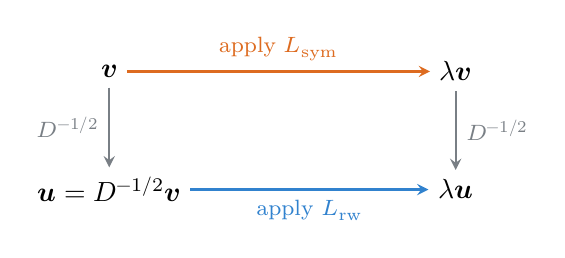
\begin{tikzpicture}[>=stealth, x=1cm, y=1cm, lab/.style={font=\footnotesize}]
\node (v) at (0,1.5) {$\vv$};
\node (lv) at (4.4,1.5) {$\lambda\vv$};
\node (u) at (0,0) {$\vu=D^{-1/2}\vv$};
\node (lu) at (4.4,0) {$\lambda\vu$};
\draw[->, thick, accentC] (v) -- node[lab, above] {apply $L_{\mathrm{sym}}$} (lv);
\draw[->, thick, dataC] (u) -- node[lab, below] {apply $L_{\mathrm{rw}}$} (lu);
\draw[->, thick, ink!60] (v) -- node[lab, left] {$D^{-1/2}$} (u);
\draw[->, thick, ink!60] (lv) -- node[lab, right] {$D^{-1/2}$} (lu);
\end{tikzpicture}
\end{center}
Both paths from $\vv$ to $\lambda\vu$ give the same answer. The two matrices are one operation written in two sets of coordinates: stretching by $\lambda$ does not depend on the coordinates, while the eigenvector does.

\textbf{Check on the path $1-2-3$,} where $D=\diag(1,2,1)$. Entry by entry, $(D^{-1/2}L_{\mathrm{sym}}D^{1/2})_{ij}=\sqrt{D_{jj}/D_{ii}}\,(L_{\mathrm{sym}})_{ij}$. For example, entry $(1,2)$ is $\sqrt2\cdot\big({-}\tfrac1{\sqrt2}\big)=-1$ and entry $(2,1)$ is $\tfrac1{\sqrt2}\cdot\big({-}\tfrac1{\sqrt2}\big)=-\tfrac12$, which gives
\[
L_{\mathrm{rw}}=\begin{bmatrix}1&-1&0\\-\tfrac12&1&-\tfrac12\\0&-1&1\end{bmatrix},\qquad
L_{\mathrm{rw}}\begin{bmatrix}1\\1\\1\end{bmatrix}=\bm0,\quad
L_{\mathrm{rw}}\begin{bmatrix}1\\0\\-1\end{bmatrix}=1\begin{bmatrix}1\\0\\-1\end{bmatrix},\quad
L_{\mathrm{rw}}\begin{bmatrix}1\\-1\\1\end{bmatrix}=2\begin{bmatrix}1\\-1\\1\end{bmatrix}.
\]
The eigenvalues $\{0,1,2\}$ match those of $L_{\mathrm{sym}}$ in Example~\ref{ex:lepath}.
\end{example}

\begin{careful}
\textbf{``Similar'' does not \emph{mean} ``same eigenvalues.''} Similar matrices always have the same eigenvalues, but the converse fails: $\left[\begin{smallmatrix}0&1\\0&0\end{smallmatrix}\right]$ and the zero matrix both have only the eigenvalue $0$, yet $CTC^{-1}=0$ whenever $T=0$, so they are not similar. Similarity is the sufficient condition this proof needs.
\textbf{A useful consequence.} $L_{\mathrm{rw}}$ is not symmetric, so on its own it could have had complex eigenvalues or too few eigenvectors. Being similar to the symmetric PSD matrix $L_{\mathrm{sym}}$ rules out both: its eigenvalues are real and nonnegative, and it is diagonalizable. Its eigenvectors are just not orthogonal in the usual dot product. They are orthogonal in the $D$-weighted one, $\vu_j\T D\vu_k=\vv_j\T\vv_k=0$, which is the off-diagonal part of $Y\T DY=I_t$.
\end{careful}

\begin{center}
\renewcommand{\arraystretch}{1.35}
\small
\begin{tabular}{>{\raggedright\arraybackslash}p{3.3cm}>{\centering\arraybackslash}p{2.7cm}>{\centering\arraybackslash}p{3.3cm}>{\centering\arraybackslash}p{4.2cm}}
\toprule
& Unnormalized $L$ & Random walk $L_{\mathrm{rw}}$ & Symmetric normalized $L_{\mathrm{sym}}$\\
\midrule
Formula & $D-A$ & $D^{-1}L=I-D^{-1}A$ & $D^{-1/2}LD^{-1/2}=I-D^{-1/2}AD^{-1/2}$\\
Symmetric? & yes & \textbf{no} & yes\\
Eigenvector for $\lambda=0$ & $\one_N$ & $\one_N$ & $D^{1/2}\one_N$\\
Eigenvalues & its own & \multicolumn{2}{c}{the same as each other (generalized problem $L\vu=\lambda D\vu$)}\\
Used for & the objective $\tr(Y\T LY)$ & interpretation (random walk) & computation (spectral theorem)\\
\bottomrule
\end{tabular}
\end{center}

\subsubsection*{What $L_{\mathrm{rw}}$ does to a function on the graph}

A \textbf{function on the graph}, $\bm f$, assigns one number to each vertex, so it is simply a vector in $\R^N$. It could be a temperature at each vertex, a class-label score, or one coordinate of the embedding (one column of $Y$). The formula that explains $L_{\mathrm{rw}}$ comes from distributing:
\[
L_{\mathrm{rw}}\bm f=(I-P)\bm f=\bm f-P\bm f,
\qquad\text{so}\qquad
\boxed{(L_{\mathrm{rw}}\bm f)_i=f_i-\sum_jP_{ij}f_j}
\]
which reads ``my value minus the weighted average of my neighbors.''

\begin{example}{The random-walk Laplacian on five vertices, from the start}{rwfive}
Take vertices $a,b,c,d,e$ with edge strengths $a{-}b=\tfrac12$, $a{-}c=\tfrac12$, $b{-}c=\tfrac14$, $b{-}d=\tfrac14$, $c{-}e=\tfrac14$, $d{-}e=\tfrac12$ (Figure~\ref{fig:rwfive}(a)). Each row of $A$ lists one vertex's edge strengths, its total goes on the diagonal of $D$, and dividing each row by that total gives $P=D^{-1}A$:
\[
A=\begin{bmatrix}0&\frac12&\frac12&0&0\\\frac12&0&\frac14&\frac14&0\\\frac12&\frac14&0&0&\frac14\\0&\frac14&0&0&\frac12\\0&0&\frac14&\frac12&0\end{bmatrix},
\quad
D=\diag\big(1,1,1,\tfrac34,\tfrac34\big),
\quad
P=\begin{bmatrix}0&\frac12&\frac12&0&0\\\frac12&0&\frac14&\frac14&0\\\frac12&\frac14&0&0&\frac14\\0&\frac13&0&0&\frac23\\0&0&\frac13&\frac23&0\end{bmatrix}.
\]
Row $d$ shows the division: $\big[0,\tfrac14,0,0,\tfrac12\big]\div\tfrac34=\big[0,\tfrac13,0,0,\tfrac23\big]$. Every row of $P$ sums to $1$.

Now put the values $\bm f=(2,4,3,10,7)\T$ on the vertices. At $d$,
\[
(P\bm f)_d=\tfrac13f_b+\tfrac23f_e=\tfrac13(4)+\tfrac23(7)=6,
\qquad
(L_{\mathrm{rw}}\bm f)_d=f_d-(P\bm f)_d=10-6=4 .
\]
So $d$'s value is $4$ above the average of its neighbors. Doing this at every vertex:
\begin{center}
\renewcommand{\arraystretch}{1.25}
\begin{tabular}{lccccc}
\toprule
vertex & $a$ & $b$ & $c$ & $d$ & $e$\\
\midrule
$f_i$ & $2$ & $4$ & $3$ & $10$ & $7$\\
$(P\bm f)_i$, neighbor average & $\tfrac72$ & $\tfrac{17}4$ & $\tfrac{15}4$ & $6$ & $\tfrac{23}3$\\
$(L_{\mathrm{rw}}\bm f)_i$, mismatch & $-\tfrac32$ & $-\tfrac14$ & $-\tfrac34$ & $4$ & $-\tfrac23$\\
\bottomrule
\end{tabular}
\end{center}
\emph{Check:} the degree-weighted mismatches cancel, $1\big({-}\tfrac32-\tfrac14-\tfrac34\big)+\tfrac34\big(4-\tfrac23\big)=-\tfrac52+\tfrac52=0$. They must, since $\one\T DL_{\mathrm{rw}}\bm f=\one\T L\bm f=0$.
\end{example}

\begin{figure}[htbp]
\centering
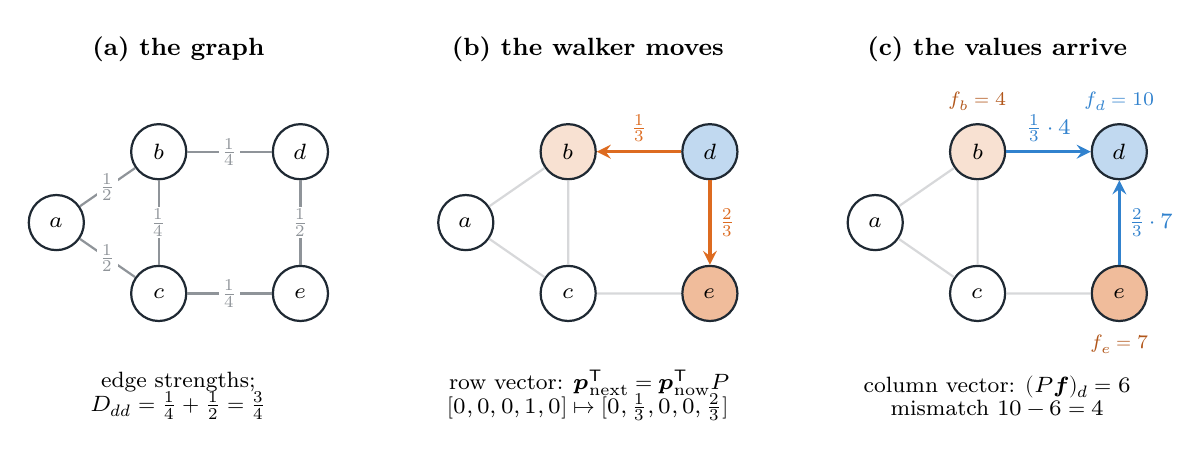
\begin{tikzpicture}[>=stealth,
  v/.style={circle,draw=ink,thick,fill=white,minimum size=7mm,inner sep=0pt,font=\footnotesize},
  w/.style={font=\footnotesize,fill=white,inner sep=0.8pt},
  ed/.style={ink!50,thick}, faint/.style={ink!18,thick}]
\newcommand{\gnodes}[5]{%
  \node[v,#1] (a) at (0,1) {$a$}; \node[v,#2] (b) at (1.3,1.9) {$b$}; \node[v,#3] (c) at (1.3,0.1) {$c$};
  \node[v,#4] (d) at (3.1,1.9) {$d$}; \node[v,#5] (e) at (3.1,0.1) {$e$};}
\begin{scope}
  \node[font=\small\bfseries] at (1.55,3.2) {(a) the graph};
  \gnodes{}{}{}{}{}
  \draw[ed] (a)--node[w]{$\tfrac12$}(b); \draw[ed] (a)--node[w]{$\tfrac12$}(c); \draw[ed] (b)--node[w]{$\tfrac14$}(c);
  \draw[ed] (b)--node[w]{$\tfrac14$}(d); \draw[ed] (c)--node[w]{$\tfrac14$}(e); \draw[ed] (d)--node[w]{$\tfrac12$}(e);
  \node[font=\footnotesize,align=center] at (1.55,-1.2) {edge strengths;\\[-1pt]$D_{dd}=\tfrac14+\tfrac12=\tfrac34$};
\end{scope}
\begin{scope}[xshift=5.2cm]
  \node[font=\small\bfseries] at (1.55,3.2) {(b) the walker moves};
  \gnodes{}{fill=accentC!20}{}{fill=dataC!30}{fill=accentC!45}
  \draw[faint] (a)--(b) (a)--(c) (b)--(c) (c)--(e);
  \draw[->,very thick,accentC] (d)--node[w,above=2pt]{$\tfrac13$}(b);
  \draw[->,very thick,accentC] (d)--node[w,right=2pt]{$\tfrac23$}(e);
  \node[font=\footnotesize,align=center] at (1.55,-1.2) {row vector: $\bm p\T_{\text{next}}=\bm p\T_{\text{now}}P$\\[-1pt]$[0,0,0,1,0]\mapsto[0,\tfrac13,0,0,\tfrac23]$};
\end{scope}
\begin{scope}[xshift=10.4cm]
  \node[font=\small\bfseries] at (1.55,3.2) {(c) the values arrive};
  \gnodes{}{fill=accentC!20}{}{fill=dataC!30}{fill=accentC!45}
  \draw[faint] (a)--(b) (a)--(c) (b)--(c) (c)--(e);
  \draw[->,very thick,dataC] (b)--node[w,above=2pt]{$\tfrac13\cdot4$}(d);
  \draw[->,very thick,dataC] (e)--node[w,right=2pt]{$\tfrac23\cdot7$}(d);
  \node[font=\scriptsize,accentC!80!black,above=1pt] at (b.north) {$f_b=4$};
  \node[font=\scriptsize,accentC!80!black,below=1pt] at (e.south) {$f_e=7$};
  \node[font=\scriptsize,dataC,above=1pt] at (d.north) {$f_d=10$};
  \node[font=\footnotesize,align=center] at (1.55,-1.2) {column vector: $(P\bm f)_d=6$\\[-1pt]mismatch $10-6=4$};
\end{scope}
\end{tikzpicture}
\caption{Two ways to read the same matrix $P$. Multiplying a probability row vector on the \emph{left} moves the walker forward along the edges (b). Multiplying a value column vector on the \emph{right} pulls values backward along the same edges (c). They are linked: $(P\bm f)_d$ is the expected value of $f$ after one step of a walker starting at $d$.}
\label{fig:rwfive}
\end{figure}

\begin{careful}
\textbf{``Mismatch $=0$'' at one vertex does not mean its neighbors look like it.} It only means the value equals the weighted average of its neighbors. With $f_d=10$, the wild values $f_b=-20$ and $f_e=25$ also give $\tfrac13(-20)+\tfrac23(25)=10$, so the mismatch at $d$ is $0$. Agreement comes only from asking this at \emph{every} vertex: on a connected graph, $L_{\mathrm{rw}}\bm f=\bm0$ forces $\bm f$ to be constant. (A vertex holding the maximum equals an average of its neighbors, so they must hold the maximum too, and this spreads across the graph.)
\textbf{Signs.} $L_{\mathrm{rw}}$ is not a probability matrix: its rows sum to $0$, not $1$. Its off-diagonal entries are $-P_{ij}$, so they are negative for neighbors and $0$ for non-neighbors.
\end{careful}

\textbf{Why this matters: the eigenvector equation in words.} $L_{\mathrm{rw}}\vu=\lambda\vu$ is the same as $P\vu=(1-\lambda)\vu$: at every vertex, the neighbor average equals $(1-\lambda)$ times the vertex's own value. A small $\lambda$ therefore means each value is almost its own neighbor average, which is smoothness stated locally. On this graph $\lambda_2\approx0.463$ and, up to sign, $\vu_2\approx(-0.474,-0.255,-0.255,0.656,0.656)\T$. At $d$: $\tfrac13(-0.255)+\tfrac23(0.656)\approx0.352\approx(1-0.463)(0.656)$. The sign of $\vu_2$ splits $\{a,b,c\}$ from $\{d,e\}$, which is the weak link in the graph: only $b{-}d$ and $c{-}e$ cross, with strength $\tfrac14$ each.

\begin{figure}[htbp]
\centering
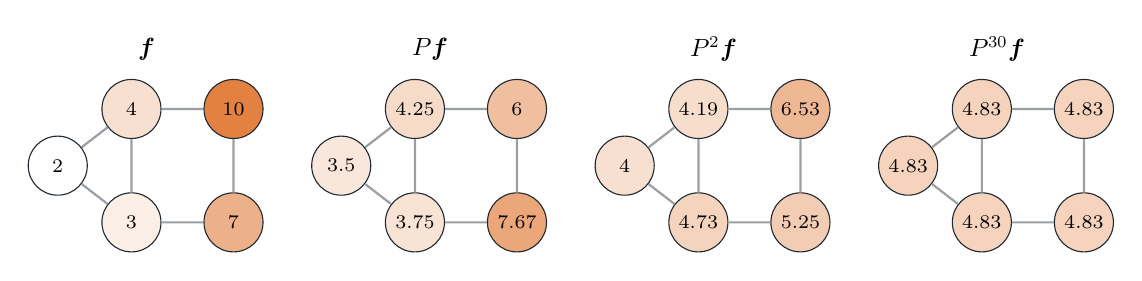
\begin{tikzpicture}[x=0.72cm,y=0.72cm,
  v/.style={circle,draw=ink,minimum size=7.5mm,inner sep=0pt,font=\scriptsize},
  ed/.style={ink!45,thick}]
\newcommand{\smooth}[3]{%
  \begin{scope}[xshift=#1cm]
    \node[font=\small\bfseries] at (1.55,3.05) {#2};
    \foreach \name/\x/\y/\val/\pct in {#3}{\node[v,fill=accentC!\pct!white] (\name) at (\x,\y) {\val};}
    \draw[ed] (a)--(b) (a)--(c) (b)--(c) (b)--(d) (c)--(e) (d)--(e);
  \end{scope}}
\smooth{0}{$\bm f$}{a/0/1/2/0,b/1.3/2/4/21,c/1.3/0/3/11,d/3.1/2/10/85,e/3.1/0/7/53}
\smooth{3.6}{$P\bm f$}{a/0/1/3.5/16,b/1.3/2/4.25/24,c/1.3/0/3.75/19,d/3.1/2/6/43,e/3.1/0/7.67/60}
\smooth{7.2}{$P^2\bm f$}{a/0/1/4/21,b/1.3/2/4.19/23,c/1.3/0/4.73/29,d/3.1/2/6.53/48,e/3.1/0/5.25/34}
\smooth{10.8}{$P^{30}\bm f$}{a/0/1/4.83/30,b/1.3/2/4.83/30,c/1.3/0/4.83/30,d/3.1/2/4.83/30,e/3.1/0/4.83/30}
\end{tikzpicture}
\caption{Applying $P$ again and again replaces every value by a neighbor average, so differences die out, like heat spreading. On this graph the values settle at the degree-weighted mean, $\sum_iD_{ii}f_i/\sum_iD_{ii}=\tfrac{29}{6}\approx4.83$, which is why the constant vector has $\lambda=0$. (This needs a connected graph that is not bipartite. The triangle $a,b,c$ makes this one non-bipartite.) The slowest differences to fade are the smoothest eigenvectors, the ones Laplacian eigenmaps keeps. Values computed exactly and rounded for display; the color scale is the same in all four panels.}
\label{fig:rwsmooth}
\end{figure}

\begin{theorem}{Solution of Laplacian eigenmaps}{lesolution}
Let the graph be connected with all degrees positive. Let $0=\lambda_1<\lambda_2\le\cdots\le\lambda_N$ be the eigenvalues of $L_{\mathrm{sym}}$ with
orthonormal eigenvectors $\vv_1=D^{1/2}\one_N/\norm{D^{1/2}\one_N},\ \vv_2,\dots,\vv_N$. Then
\[
\widetilde Y=\big[\,\vv_2\ \cdots\ \vv_{t+1}\big],\qquad Y=D^{-1/2}\widetilde Y,\qquad \bm y_i=\frac{1}{\sqrt{D_{ii}}}\big(v_2(i),\dots,v_{t+1}(i)\big)\T,
\]
and the minimum value is $\tr(Y\T LY)=\tr(\widetilde Y\T L_{\mathrm{sym}}\widetilde Y)=\sum_{j=2}^{t+1}\vv_j\T L_{\mathrm{sym}}\vv_j=\lambda_2+\cdots+\lambda_{t+1}$.
\end{theorem}
\begin{proofsketch}
\emph{Feasible.} $\widetilde Y\T\widetilde Y=I_t$ because the $\vv_j$ are orthonormal. $\widetilde Y\T D^{1/2}\one_N=\bm 0$ because each of $\vv_2,\dots,\vv_{t+1}$
is orthogonal to $\vv_1\propto D^{1/2}\one_N$. This is exactly why $\vv_1$ is skipped: the centering constraint \emph{is} ``orthogonal to the first eigenvector.''
\emph{Optimal.} For a symmetric matrix, the minimum of $\tr(\widetilde Y\T M\widetilde Y)$ over $\widetilde Y\T\widetilde Y=I_t$ is the sum of the $t$
smallest eigenvalues (Ky Fan; the mirror image of PCA's maximum-variance argument, proved by hand after Example~\ref{ex:lepath}). Centering confines $\widetilde Y$ to the subspace orthogonal to
$\vv_1$, and the smallest eigenvalues there are $\lambda_2,\dots,\lambda_{t+1}$.
\end{proofsketch}

\begin{careful}
\textbf{``If the constraints forbid the constant vector, why does the solver return it?''} The constraints belong to the \emph{optimization problem}, not to the eigenproblem. The equation $L\vu=\lambda D\vu$ knows nothing about centering. The Lagrange step above used only the scaling constraint, and $\one$ genuinely solves the bare equation, since $L\one=\bm0=0\cdot D\one$. So an eigensolver returns every pair, in order of $\lambda$, and on a connected graph the first pair is
\[
\lambda_1=0,\qquad \vu_1=\frac{\one}{\sqrt{\one\T D\one}}=\begin{bmatrix}c\\\vdots\\c\end{bmatrix}\quad(\text{scaled so that }\vu_1\T D\vu_1=1).
\]
Its entries are all equal, though not literally $1$. On the chain, $\one\T D\one=4$ and $\vu_1=(\tfrac12,\tfrac12,\tfrac12)$, which is exactly the cheat from Figure~\ref{fig:pullonly}. It fails centering, $\vu_1\T D\one=c\,\one\T D\one\ne0$, so it cannot be a coordinate.

\textbf{Dropping $\vu_1$ \emph{is} how centering gets imposed.} Every other generalized eigenvector is $D$-orthogonal to $\vu_1$, and therefore satisfies $\vu_j\T D\one=0$ automatically. So you never enforce centering separately: you compute the spectrum and skip the first entry.
\begin{center}
\small
\renewcommand{\arraystretch}{1.2}
\begin{tabular}{@{}ll@{}}
\toprule
Object & The constant vector\\
\midrule
the full generalized eigensystem $L\vu=\lambda D\vu$ & present, as the first pair, with $\lambda_1=0$\\
the embedding coordinates & discarded; start from $\vu_2$\\
\bottomrule
\end{tabular}
\end{center}
For $t=2$, $Y=[\,\vu_2\ \ \vu_3\,]$, not $[\,\vu_1\ \ \vu_2\,]$, and point $i$ goes to $\bm y_i=\big(u_2(i),\,u_3(i)\big)$. If you computed eigenvectors $\vv_j$ of $L_{\mathrm{sym}}$ instead, divide by $\sqrt{D_{ii}}$ first, since $\vu_j=D^{-1/2}\vv_j$; using $v_2(i),v_3(i)$ directly gives a different picture unless all degrees are equal. And $\vu_1$ is the only constant pair only on a connected graph. With several components, $\lambda=0$ repeats, and you must skip all of the $\lambda=0$ pairs, one per component.
\end{careful}

\begin{intuition}
\textbf{The same eigen-answer as PCA, from the other end.} PCA keeps the eigenvectors of $\Sig$ with the \emph{largest} eigenvalues (most variance). Laplacian eigenmaps keeps the eigenvectors of $L_{\mathrm{sym}}$
with the \emph{smallest} eigenvalues (least roughness), after throwing away the trivial one. The answer is \textbf{nested}: the best
$(t-1)$-dimensional embedding is the best $t$-dimensional one with its last column dropped, as with PCA and classical scaling. The final
division by $\sqrt{D_{ii}}$ is the ``free to have larger magnitude'' effect: low-degree points get their eigenvector entries scaled \emph{up}.
\end{intuition}

\begin{example}{The three-vertex path, solved completely}{lepath}
Take the path $1-2-3$ from Example~\ref{ex:lappath}, with $D=\diag(1,2,1)$. Then $D^{-1/2}AD^{-1/2}=\begin{bmatrix}0&1/\sqrt2&0\\1/\sqrt2&0&1/\sqrt2\\0&1/\sqrt2&0\end{bmatrix}$,
and $L_{\mathrm{sym}}=I-D^{-1/2}AD^{-1/2}$ has
\[
\lambda_1=0,\ \vv_1=\tfrac12(1,\sqrt2,1)\T;\qquad \lambda_2=1,\ \vv_2=\tfrac1{\sqrt2}(1,0,-1)\T;\qquad \lambda_3=2,\ \vv_3=\tfrac12(1,-\sqrt2,1)\T .
\]
(Check $\vv_1$: $D^{1/2}\one=(1,\sqrt2,1)\T$, as Theorem~\ref{thm:lsymprops}(iii) predicts.) For $t=1$, $Y=D^{-1/2}\vv_2=\big(\tfrac1{\sqrt2},\,0,\,-\tfrac1{\sqrt2}\big)\T$.
\begin{itemize}[nosep]
\item Centering: $\sum_iD_{ii}y_i=1\cdot\tfrac1{\sqrt2}+2\cdot0+1\cdot\big(-\tfrac1{\sqrt2}\big)=0$. \checkmark
\item Scaling: $\sum_iD_{ii}y_i^2=\tfrac12+0+\tfrac12=1$. \checkmark
\item Objective: $\tfrac12\sum_{i,j}A_{ij}(y_i-y_j)^2=(y_1-y_2)^2+(y_2-y_3)^2=\tfrac12+\tfrac12=1=\lambda_2$. \checkmark
\end{itemize}
The degree-$2$ middle vertex lands exactly at the origin, and the degree-$1$ ends are pushed out symmetrically. The generalized eigenvalues
$\{0,1,2\}$ differ from the eigenvalues $\{0,1,3\}$ of the unnormalized $L$, as the table warns: the third generalized eigenvector is
$D^{-1/2}\vv_3=\tfrac12(1,-1,1)\T$, not $(1,-2,1)\T$.
\end{example}

\subsubsection*{Why eigenvectors solve it, and why orthonormality matters}

\textbf{One coordinate: the loss is a weighted average.} Take a single unit vector $\vu$ and write it in the orthonormal eigenbasis, $\vu=a_1\vv_1+\cdots+a_N\vv_N$. Orthonormality gives two facts at once:
\[
a_1^2+\cdots+a_N^2=\norm{\vu}^2=1,
\qquad
\vu\T L_{\mathrm{sym}}\vu=a_1^2\lambda_1+\cdots+a_N^2\lambda_N .
\]
So the loss is a weighted average of the eigenvalues, the same argument as Proposition~\ref{prop:rayleigh}. Mixing in any higher eigenvector raises the average, so the best choice puts all the weight on the smallest allowed eigenvalue. Centering forces $a_1=\vu\T\vv_1=0$, so that eigenvalue is $\lambda_2$ and the best coordinate is $\vu=\vv_2$.

\textbf{Several coordinates: each eigenvector has capacity $1$.} Let $\widetilde Y$ have orthonormal columns. Since $L_{\mathrm{sym}}=\sum_k\lambda_k\vv_k\vv_k\T$,
\[
\tr\big(\widetilde Y\T L_{\mathrm{sym}}\widetilde Y\big)=\sum_{k=1}^N\lambda_k\,p_k,\qquad\text{where } p_k=\norm{\widetilde Y\T\vv_k}^2
\]
measures how much of $\vv_k$ the embedding uses. Three facts pin down the answer:
\begin{itemize}[nosep]
\item $\sum_kp_k=t$. The $\vv_k$ form an orthonormal basis, so the $p_k$ add up to the squared lengths of the $t$ unit columns.
\item $0\le p_k\le1$. Here $p_k$ is the squared length of the projection of the unit vector $\vv_k$ onto the orthonormal columns, and a projection cannot be longer than the vector itself.
\item $p_1=0$, because centering says $\widetilde Y\T\vv_1=\bm0$.
\end{itemize}
You must spend a total of $t$, at most $1$ per eigenvalue, and the cheapest purchase fills $p_2=\cdots=p_{t+1}=1$. The loss is then $\lambda_2+\cdots+\lambda_{t+1}$, which proves the optimality claim in Theorem~\ref{thm:lesolution}.

\begin{figure}[htbp]
\centering
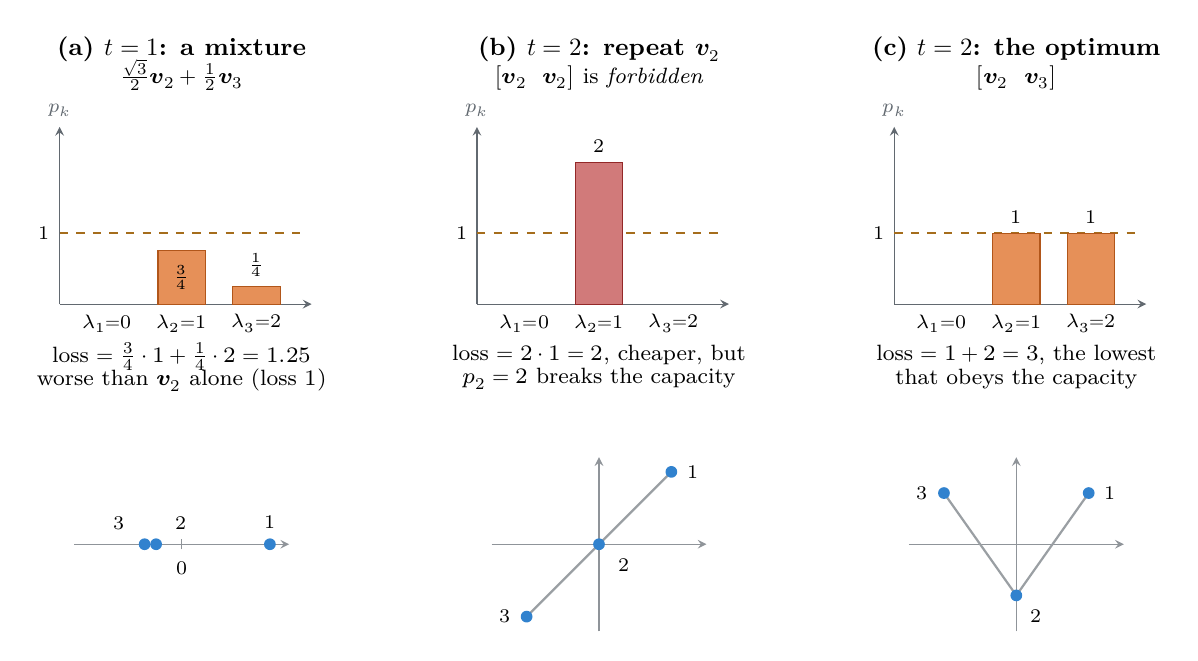
\begin{tikzpicture}[>=stealth,
  bar/.style={fill=accentC!75, draw=accentC!80!black},
  badbar/.style={fill=thmred!65, draw=thmred!80!black},
  pt/.style={circle, fill=dataC, inner sep=1.5pt},
  edge/.style={draw=ink!45, thick}]
\newcommand{\barpanel}[5]{%
  \begin{scope}[shift={(#1,0)}]
    \node[font=\small\bfseries, align=center] at (1.75,3.05) {#2};
    \draw[->, ink!70] (0.2,0) -- (3.4,0);
    \draw[->, ink!70] (0.2,0) -- (0.2,2.25) node[above, font=\scriptsize] {$p_k$};
    \draw[dashed, warnamber!90!black, thick] (0.2,0.9) -- (3.3,0.9);
    \node[font=\scriptsize, left] at (0.2,0.9) {$1$};
    #3
    \node[font=\scriptsize] at (0.8,-0.25) {$\lambda_1{=}0$};
    \node[font=\scriptsize] at (1.75,-0.25) {$\lambda_2{=}1$};
    \node[font=\scriptsize] at (2.7,-0.25) {$\lambda_3{=}2$};
    \node[font=\footnotesize, align=center] at (1.75,-0.8) {#4};
    #5
  \end{scope}}
\barpanel{0}{(a) $t=1$: a mixture\\[-1pt]\mdseries\footnotesize$\tfrac{\sqrt3}{2}\vv_2+\tfrac12\vv_3$}
  {\draw[bar] (1.45,0) rectangle (2.05,0.675); \draw[bar] (2.4,0) rectangle (3.0,0.225);
   \node[font=\scriptsize] at (1.75,0.34) {$\tfrac34$}; \node[font=\scriptsize, above] at (2.7,0.225) {$\tfrac14$};}
  {loss $=\tfrac34\cdot1+\tfrac14\cdot2=1.25$\\[-1pt]worse than $\vv_2$ alone (loss $1$)}
  {\begin{scope}[shift={(1.75,-3.05)}, x=1.3cm, y=1.3cm]
     \draw[->, ink!50] (-1.05,0) -- (1.05,0);
     \draw[ink!50] (0,-0.05) -- (0,0.05);
     \node[font=\scriptsize, below=1pt] at (0,-0.05) {$0$};
     \node[pt, label={[font=\scriptsize]above:$1$}] at (0.862,0) {};
     \node[pt, label={[font=\scriptsize, xshift=2pt]above right:$2$}] at (-0.25,0) {};
     \node[pt, label={[font=\scriptsize, xshift=-2pt]above left:$3$}] at (-0.362,0) {};
   \end{scope}}
\barpanel{5.3}{(b) $t=2$: repeat $\vv_2$\\[-1pt]\mdseries\footnotesize$\big[\vv_2\ \ \vv_2\big]$ is \emph{forbidden}}
  {\draw[badbar] (1.45,0) rectangle (2.05,1.8);
   \node[font=\scriptsize, above] at (1.75,1.8) {$2$};}
  {loss $=2\cdot1=2$, cheaper, but\\[-1pt]$p_2=2$ breaks the capacity}
  {\begin{scope}[shift={(1.75,-3.05)}, x=1.3cm, y=1.3cm]
     \draw[->, ink!50] (-1.05,0) -- (1.05,0); \draw[->, ink!50] (0,-0.85) -- (0,0.85);
     \draw[edge] (0.707,0.707) -- (0,0) -- (-0.707,-0.707);
     \node[pt, label={[font=\scriptsize]right:$1$}] at (0.707,0.707) {};
     \node[pt, label={[font=\scriptsize, xshift=2pt]below right:$2$}] at (0,0) {};
     \node[pt, label={[font=\scriptsize]left:$3$}] at (-0.707,-0.707) {};
   \end{scope}}
\barpanel{10.6}{(c) $t=2$: the optimum\\[-1pt]\mdseries\footnotesize$\big[\vv_2\ \ \vv_3\big]$}
  {\draw[bar] (1.45,0) rectangle (2.05,0.9); \draw[bar] (2.4,0) rectangle (3.0,0.9);
   \node[font=\scriptsize, above] at (1.75,0.9) {$1$}; \node[font=\scriptsize, above] at (2.7,0.9) {$1$};}
  {loss $=1+2=3$, the lowest\\[-1pt]that obeys the capacity}
  {\begin{scope}[shift={(1.75,-3.05)}, x=1.3cm, y=1.3cm]
     \draw[->, ink!50] (-1.05,0) -- (1.05,0); \draw[->, ink!50] (0,-0.85) -- (0,0.85);
     \draw[edge] (0.707,0.5) -- (0,-0.5) -- (-0.707,0.5);
     \node[pt, label={[font=\scriptsize]right:$1$}] at (0.707,0.5) {};
     \node[pt, label={[font=\scriptsize]below right:$2$}] at (0,-0.5) {};
     \node[pt, label={[font=\scriptsize]left:$3$}] at (-0.707,0.5) {};
   \end{scope}}
\end{tikzpicture}
\caption{The three-vertex path from Example~\ref{ex:lepath}. \emph{Top:} how much each panel uses each eigenvector, with the capacity $p_k\le1$ dashed. \emph{Bottom:} the resulting embedding $Y=D^{-1/2}\widetilde Y$, with the path's edges drawn in (b) and (c). In (b), two ``dimensions'' are one line drawn diagonally, and $Y\T DY=\left[\begin{smallmatrix}1&1\\1&1\end{smallmatrix}\right]\ne I_2$. In (c), $Y\T DY=I_2$ and the second axis adds new information: it separates the middle vertex from the two ends.}
\label{fig:capacity}
\end{figure}

\begin{example}{Checking panel (a) directly}{lemixture}
From the eigenvectors in Example~\ref{ex:lepath}, $\vu=\tfrac{\sqrt3}{2}\vv_2+\tfrac12\vv_3\approx(0.862,-0.354,-0.362)\T$, so $\bm y=D^{-1/2}\vu\approx(0.862,-0.250,-0.362)\T$. Then $\sum_iD_{ii}y_i\approx0.862-0.500-0.362=0$, and $\sum_iD_{ii}y_i^2\approx0.744+0.125+0.131=1$, so it is feasible. Its loss is $(y_1-y_2)^2+(y_2-y_3)^2\approx1.237+0.013=1.25$, which is exactly the weighted average $\tfrac34\lambda_2+\tfrac14\lambda_3$ and worse than the optimum $\lambda_2=1$.
\end{example}

\begin{careful}
\textbf{Orthonormal, not just independent.} Linear independence would not be enough. The columns $\vv_2$ and $0.99\,\vv_2+0.14\,\vv_3$ are independent, yet the second nearly repeats the first, and the picture is nearly a line. Orthogonality is what forces a genuinely new direction, and it is also what makes the capacity bound $p_k\le1$ true.
\textbf{The optimum is a subspace, not a unique matrix.} $[\vv_2,\dots,\vv_{t+1}]$ is the standard answer, but $\widetilde YQ$ for orthogonal $Q$ has the same $p_k$ and the same loss (blind spot (c)). When eigenvalues repeat, there are further ties between eigenvectors.
\end{careful}

\begin{intuition}
\textbf{The whole method in one sentence.} Among all embeddings with a fixed weighted center and a fixed weighted scale, find the one where graph neighbors change coordinate as little as possible. The answer is the smoothest non-constant functions on the graph: $\vv_2$ varies as gently as possible across strong edges, and each later eigenvector is the next-smoothest direction that is orthogonal to the earlier ones. Orthonormality does two jobs here: it fixes the scale, and it turns ``find $t$ different smooth directions'' into a precise constraint.
\end{intuition}

\begin{center}
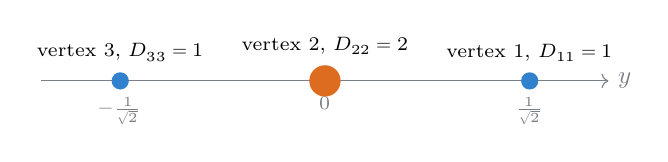
\begin{tikzpicture}[scale=1.0]
\draw[->,thin,ink!60] (-3.6,0) -- (3.6,0) node[right,font=\small]{$y$};
\foreach \x/\l in {-2.6/{-\tfrac1{\sqrt2}},0/0,2.6/{\tfrac1{\sqrt2}}} \draw[ink!60] (\x,0.08)--(\x,-0.08) node[below,font=\scriptsize]{$\l$};
\node[circle,fill=dataC,inner sep=2.2pt,label={[font=\scriptsize]above:{vertex 3, $D_{33}=1$}}] at (-2.6,0) {};
\node[circle,fill=accentC,inner sep=4.0pt,label={[font=\scriptsize]above:{vertex 2, $D_{22}=2$}}] at (0,0) {};
\node[circle,fill=dataC,inner sep=2.2pt,label={[font=\scriptsize]above:{vertex 1, $D_{11}=1$}}] at (2.6,0) {};
\end{tikzpicture}

{\small The 1-D embedding of the path (dot size $\propto$ degree). The high-degree point sits at the origin.}
\end{center}

\textbf{An uneven graph.} On the path above, the symmetry makes things tidy. Figure~\ref{fig:change} repeats the calculation on a graph with uneven degrees, to show what the rescaling $\bm y_i=\vv(i)/\sqrt{D_{ii}}$ does.

\begin{figure}[htbp]
\centering
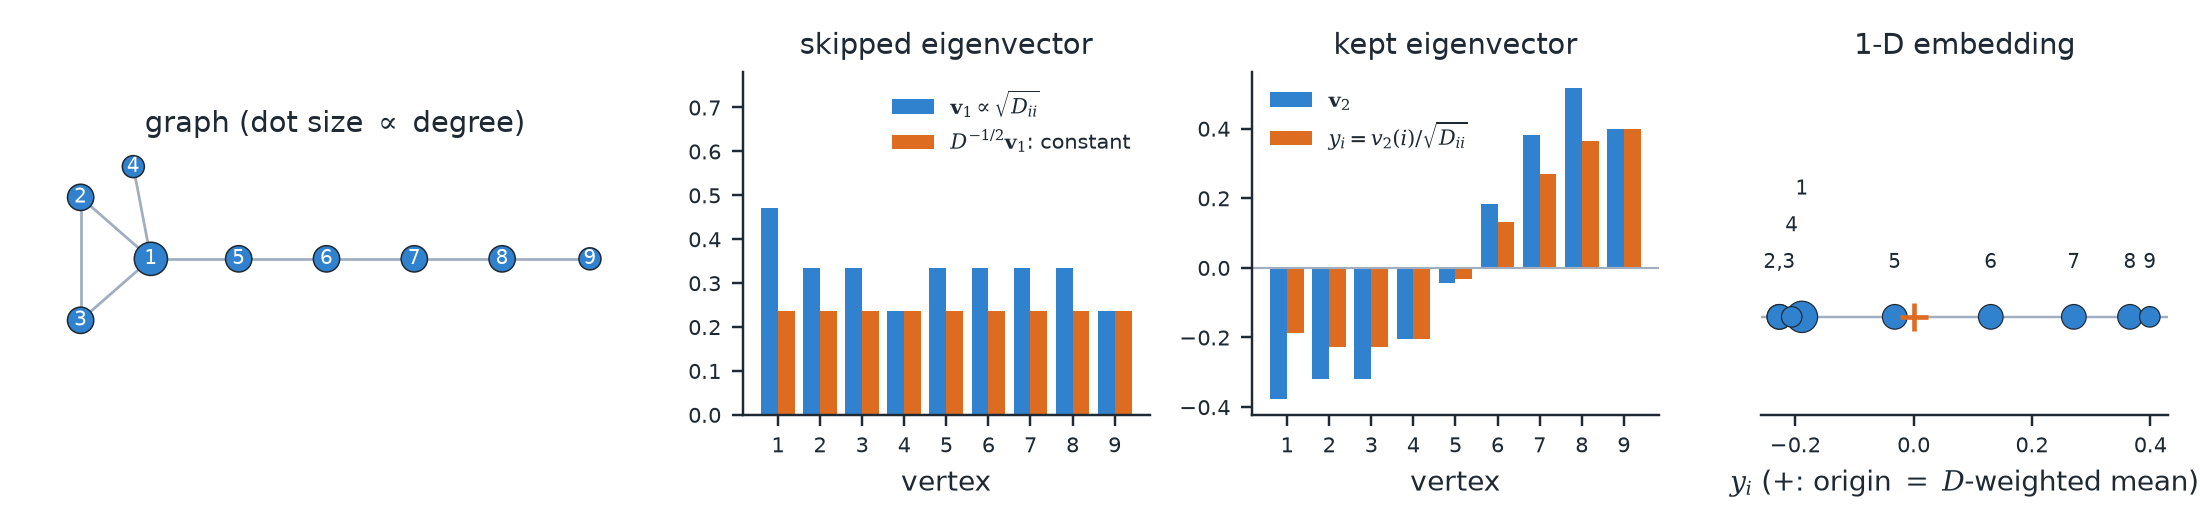
\includegraphics[width=\textwidth]{figures/lap_change.png}
\caption{A triangle-with-a-tail graph, degrees $(4,2,2,1,2,2,2,2,1)$. \emph{Skipped eigenvector:} $\bm v_1\propto\sqrt{D_{ii}}$ looks uneven, but $D^{-1/2}$ turns it into a constant: it is the trivial ``everyone at one point'' solution. \emph{Kept eigenvector:} dividing by $\sqrt{D_{ii}}$ shrinks high-degree entries most. Vertex $9$ (degree $1$) becomes the most extreme point even though $\bm v_2$ is largest at vertex $8$. \emph{Embedding:} the constraints hold ($\sum_iD_{ii}y_i=0$, $\sum_iD_{ii}y_i^2=1$), and $\lambda_2=0.084$. Note vertex $1$: it has the highest degree but is \emph{not} nearest the origin, because the tail pulls the weighted center away from it. High degree favors the origin only as a tendency.}
\label{fig:change}
\end{figure}

\begin{algorithm}{Laplacian eigenmaps}{lapeig}
Input: $\vx_1,\dots,\vx_N\in\R^d$, target dimension $t$, neighborhood size $k$ (or $\varepsilon$), bandwidth $\sigma$.
\begin{enumerate}[nosep]
\item Build the neighbor graph ($k$-NN with the ``or'' rule, or $\varepsilon$-ball). Check that it is connected.
\item Set $A_{ij}=e^{-\norm{\vx_i-\vx_j}^2/\sigma^2}$ for $j\in N_i$ and $0$ otherwise. Form $D=\diag(A\one)$, $L=D-A$ and $L_{\mathrm{sym}}=D^{-1/2}LD^{-1/2}$ (all sparse).
\item Compute the $t+1$ smallest eigenpairs of $L_{\mathrm{sym}}$. Discard $\vv_1\propto D^{1/2}\one$, and keep $\vv_2,\dots,\vv_{t+1}$.
\item Output $Y=D^{-1/2}[\vv_2\cdots\vv_{t+1}]$. Row $i$ is the embedding $\bm y_i\in\R^t$ of $\vx_i$.
\end{enumerate}
\end{algorithm}

\subsubsection*{Why the Swiss roll comes out as an arch}

If eigenvectors are waves, then which coordinates the method picks is a question of which wave is cheapest. On the roll, the answer explains a surprise in the comparison later (Figure~\ref{fig:umapcompare}): two coordinates do not give a flat rectangle, but an arch.

\begin{figure}[htbp]
\centering
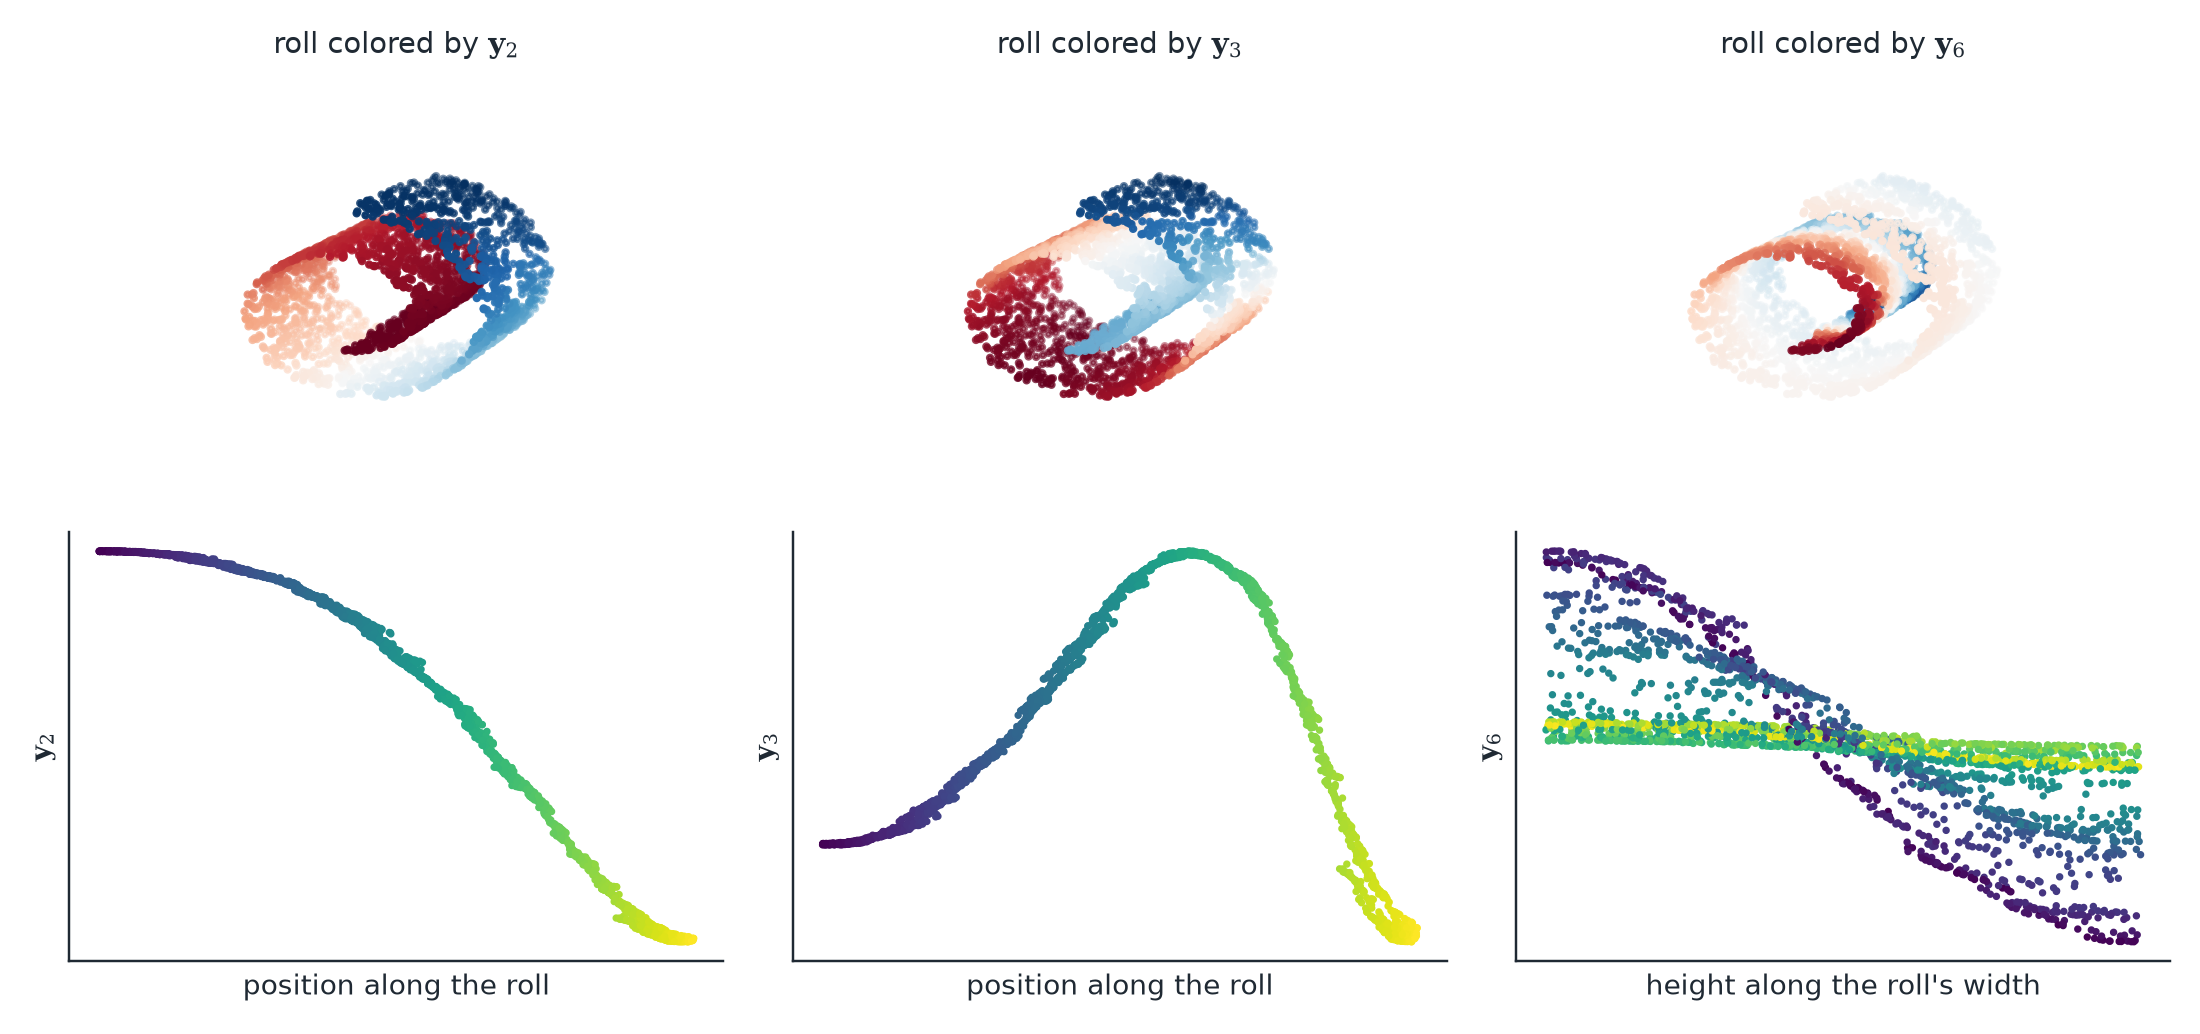
\includegraphics[width=\textwidth]{figures/lap_roll.png}
\caption{Real eigenvectors on a $2500$-point Swiss roll ($k=12$), with $\bm y_j=D^{-1/2}\bm v_j$. $\bm y_2$ is one wave along the roll, and $\bm y_3$ is a second wave \emph{along the same direction}: both are functions of position on the roll, so plotting $\bm y_3$ against $\bm y_2$ traces a single curve, the arch. The roll is about $89$ long and $21$ wide, so a wave across its width costs about as much as the $4.2$-th wave along it. The first coordinate that responds to width duly arrives late: the correlation with height is at most $0.13$ for $\bm y_2,\dots,\bm y_5$ and jumps to $0.74$ at $\bm y_6$, where it is strongest on the inner part of the roll (dark purple).}
\label{fig:roll}
\end{figure}

\begin{careful}
\textbf{Smallest eigenvalues do not mean independent coordinates.} PCA's components are uncorrelated, and on a flat rectangle you might expect ``length'' and ``width'' as the first two eigenmaps. But the eigenvectors are only orthogonal \emph{as vectors}. $\bm y_3$ can be, and here nearly is, a deterministic function of $\bm y_2$. Keeping $t=2$ loses the width of the roll entirely, even though the manifold is 2-D.
\end{careful}

\subsubsection*{What the eigenvalues tell you}

\textbf{1. Zero eigenvalues count clusters.} The multiplicity of the eigenvalue $0$ (for $L$, $L_{\mathrm{rw}}$ and $L_{\mathrm{sym}}$ alike) equals the
number of connected components of the graph. \why $\vz\T L\vz=\tfrac12\sum_{i,j}A_{ij}(z_i-z_j)^2=0$ forces $z_i=z_j$ across every edge, so $\vz$ is
constant on each component, and it can take a different constant on each one. With $c$ components, the indicator vectors $\one_{C_1},\dots,\one_{C_c}$
span the null space. \sowhat If $\lambda_2\approx0$, your graph has fallen apart: the outlier $f$ in Figure~\ref{fig:epsknn}, or $k$ or $\varepsilon$
too small. The ``embedding'' $\vv_2$ is then just a component indicator, so every component collapses to a single point. That is useless for
manifold learning, and it is exactly what \textbf{spectral clustering} exploits on purpose.

\begin{figure}[htbp]
\centering
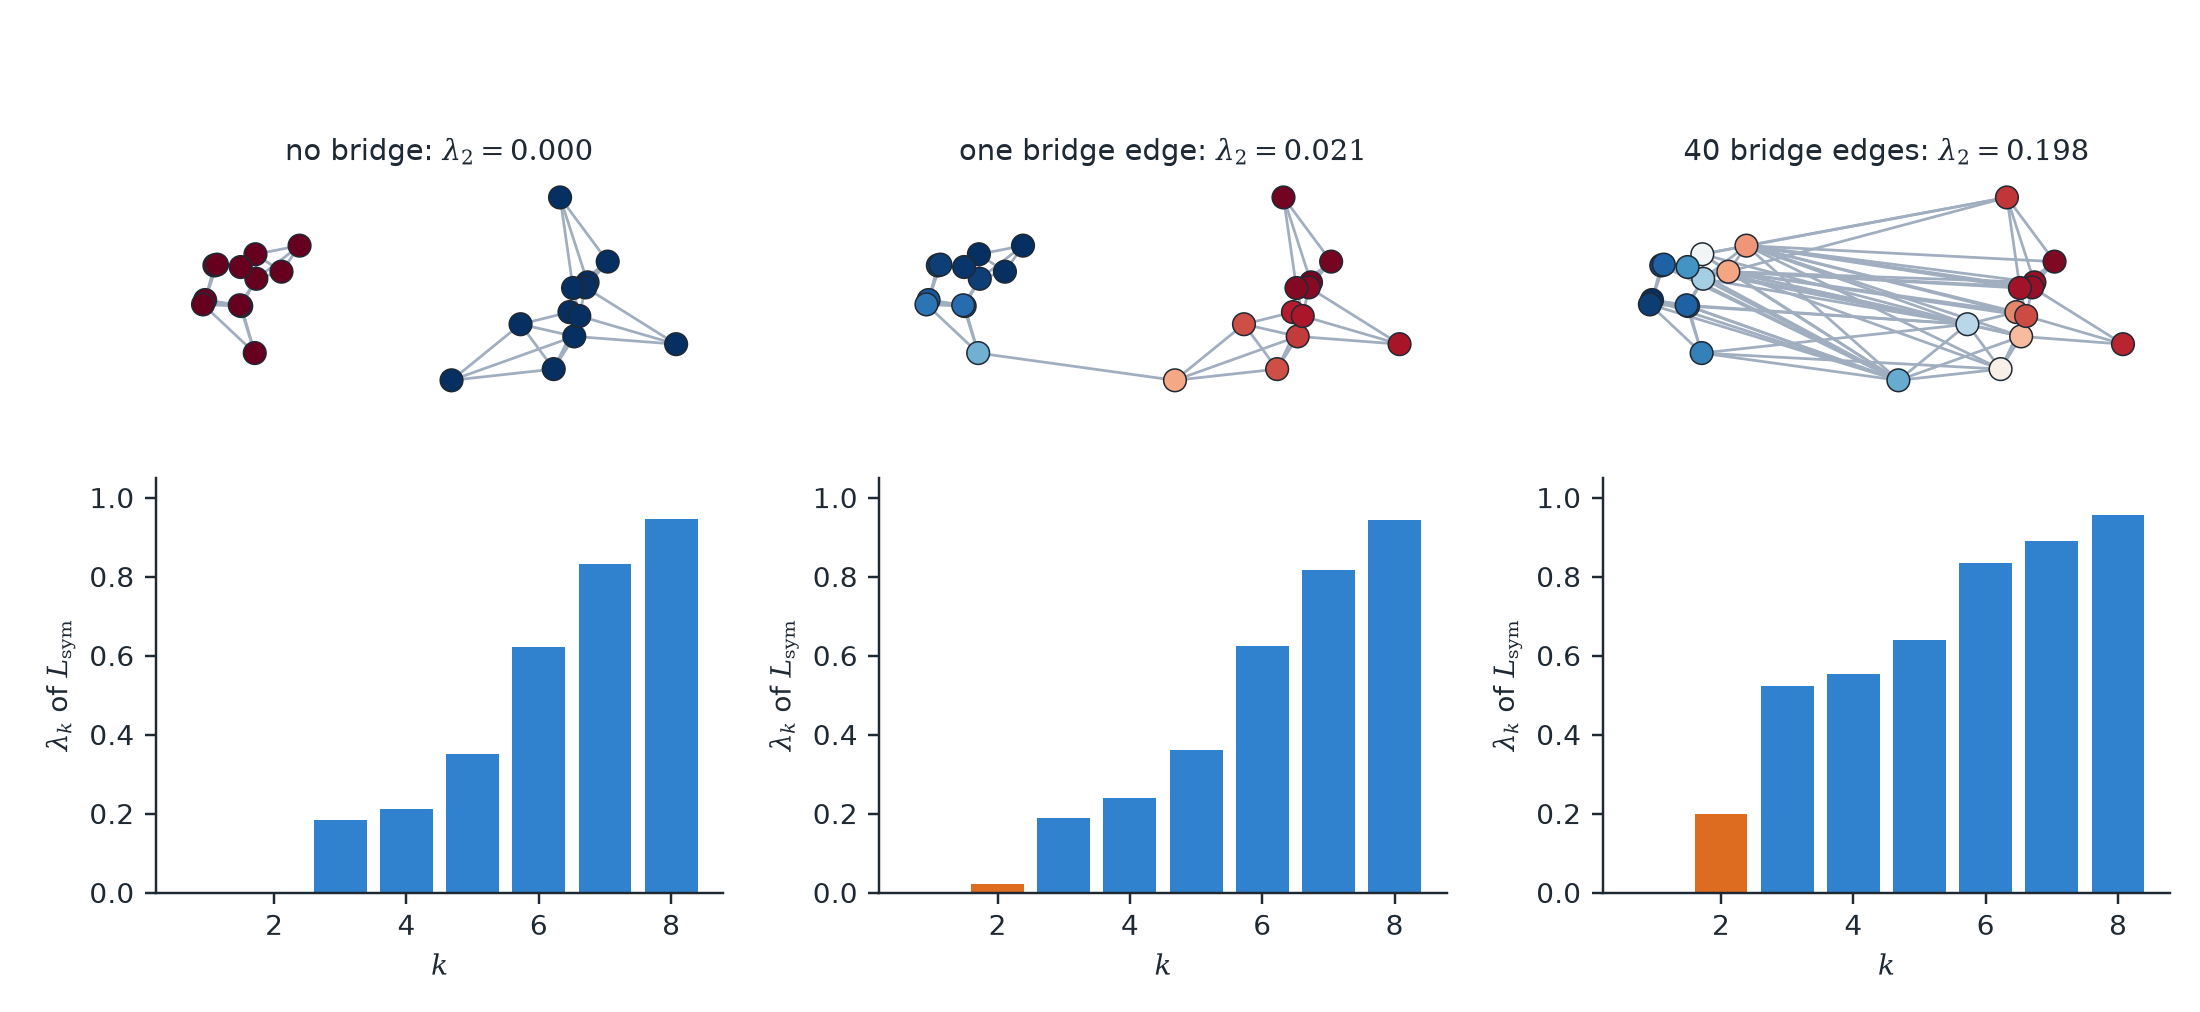
\includegraphics[width=\textwidth]{figures/lap_clusters.png}
\caption{Two clusters joined by $0$, $1$ or $40$ edges, with vertices colored by the embedding coordinate $\bm y_2$ and the first eight eigenvalues of $L_{\mathrm{sym}}$ below. \emph{No bridge:} $\lambda_1=\lambda_2=0$, one zero per component, and each cluster collapses to a single value. \emph{One bridge:} $\lambda_2$ lifts only slightly, to $0.021$, with a clear gap before $\lambda_3=0.189$, and the coordinate now varies smoothly across the bridge. \emph{Many bridges:} $\lambda_2=0.198$ and the clusters blend. A small $\lambda_2$ followed by a jump says ``two nearly separate pieces.''}
\label{fig:clusters}
\end{figure}

\textbf{2. The eigenvalue growth estimates intrinsic dimension.} Plot $\log\lambda_k$ against $\log k$. Over a middle range of $k$ it is close to a line with
\[
\text{slope}\ \approx\ \frac{2}{t},\qquad t=\text{intrinsic dimension of the manifold}.
\]

\begin{figure}[htbp]
\centering
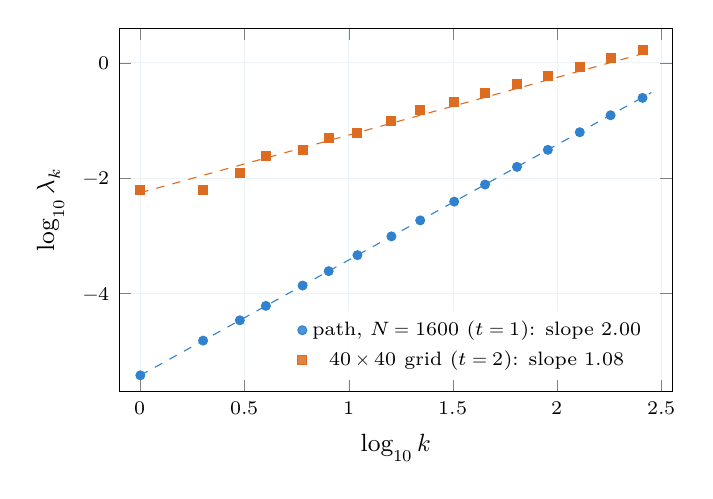
\begin{tikzpicture}
\begin{axis}[width=8.6cm,height=6.2cm,
  xlabel={$\log_{10} k$}, ylabel={$\log_{10}\lambda_k$},
  xmin=-0.1,xmax=2.55, ymin=-5.7, ymax=0.6,
  legend pos=south east, legend style={font=\scriptsize,draw=none,fill=white,fill opacity=0.85,text opacity=1},
  tick label style={font=\scriptsize}, label style={font=\small}, grid=major, grid style={softgray}]
\addplot[only marks,mark=*,mark size=1.6pt,dataC] coordinates {(0.000,-5.414) (0.301,-4.812) (0.477,-4.460) (0.602,-4.210) (0.778,-3.858) (0.903,-3.608) (1.041,-3.331) (1.204,-3.006) (1.342,-2.729) (1.505,-2.404) (1.653,-2.108) (1.806,-1.802) (1.954,-1.507) (2.107,-1.202) (2.255,-0.908) (2.408,-0.607)};
\addlegendentry{path, $N=1600$ ($t=1$): slope $2.00$}
\addplot[only marks,mark=square*,mark size=1.6pt,accentC] coordinates {(0.000,-2.210) (0.301,-2.210) (0.477,-1.909) (0.602,-1.609) (0.778,-1.512) (0.903,-1.308) (1.041,-1.212) (1.204,-1.009) (1.342,-0.817) (1.505,-0.683) (1.653,-0.522) (1.806,-0.361) (1.954,-0.222) (2.107,-0.069) (2.255,0.076) (2.408,0.224)};
\addlegendentry{$40\times40$ grid ($t=2$): slope $1.08$}
\addplot[dataC,thin,dashed,domain=0:2.45] {-5.414+2*x};
\addplot[accentC,thin,dashed,domain=0:2.45] {-2.25+1*x};
\end{axis}
\end{tikzpicture}
\caption{Real Laplacian eigenvalues for a 1-D graph (a path) and a 2-D graph (a grid). Here $k$ indexes the non-zero eigenvalues ($\lambda_2,\lambda_3,\dots$
relabeled $1,2,\dots$). Least-squares slopes are $2.00\approx2/1$ and $1.08\approx2/2$. The grid's repeated eigenvalues (its symmetry) make the steps.}
\label{fig:weyl}
\end{figure}

\begin{intuition}
\textbf{Why the slope is $2/t$ (Weyl's law).} The eigenvectors with small $\lambda$ are smooth ``waves'' over the manifold, and $\lambda$ measures how wiggly they are. On a $t$-dimensional patch of
side $\ell$, the waves look like $\sin(\pi\bm n\cdot\bm u/\ell)$ for an integer frequency vector $\bm n\in\mathbb Z^t$, with eigenvalue $\propto\norm{\bm n}^2$.
The number of frequency vectors with $\norm{\bm n}\le r$ is the number of lattice points in a $t$-dimensional ball, $\propto r^t$. So the $k$-th
eigenvalue has $\norm{\bm n}\propto k^{1/t}$, and therefore
\[
\lambda_k\propto k^{2/t}\quad\Longrightarrow\quad\log\lambda_k\approx\tfrac{2}{t}\log k+\text{const}.
\]
Check on the path: $\lambda_k=2-2\cos(\pi k/N)\approx(\pi k/N)^2$, slope $2$, so $t=1$. In 2-D there are many more slow waves (every direction gives one),
so eigenvalues pile up and grow only linearly.
\end{intuition}

\begin{careful}
\begin{itemize}[nosep,leftmargin=*]
\item \textbf{Two different $t$'s.} In the slope $2/t$, $t$ is the \emph{intrinsic} dimension of the manifold (Section~\ref{sec:manifold}). It is not the number of
eigenvectors you choose to keep, although ideally you would keep exactly that many.
\item \textbf{Only a sanity check.} The law is asymptotic and assumes RBF/heat-kernel weights, roughly uniform sampling and a graph fine enough to resolve the waves.
Very small $k$ is noisy and very large $k$ saturates at the graph's resolution. It is less robust than local PCA (Section~\ref{sec:localpca}), so use it to
confirm an estimate, not as the estimate.
\end{itemize}
\end{careful}

\begin{figure}[htbp]
\centering
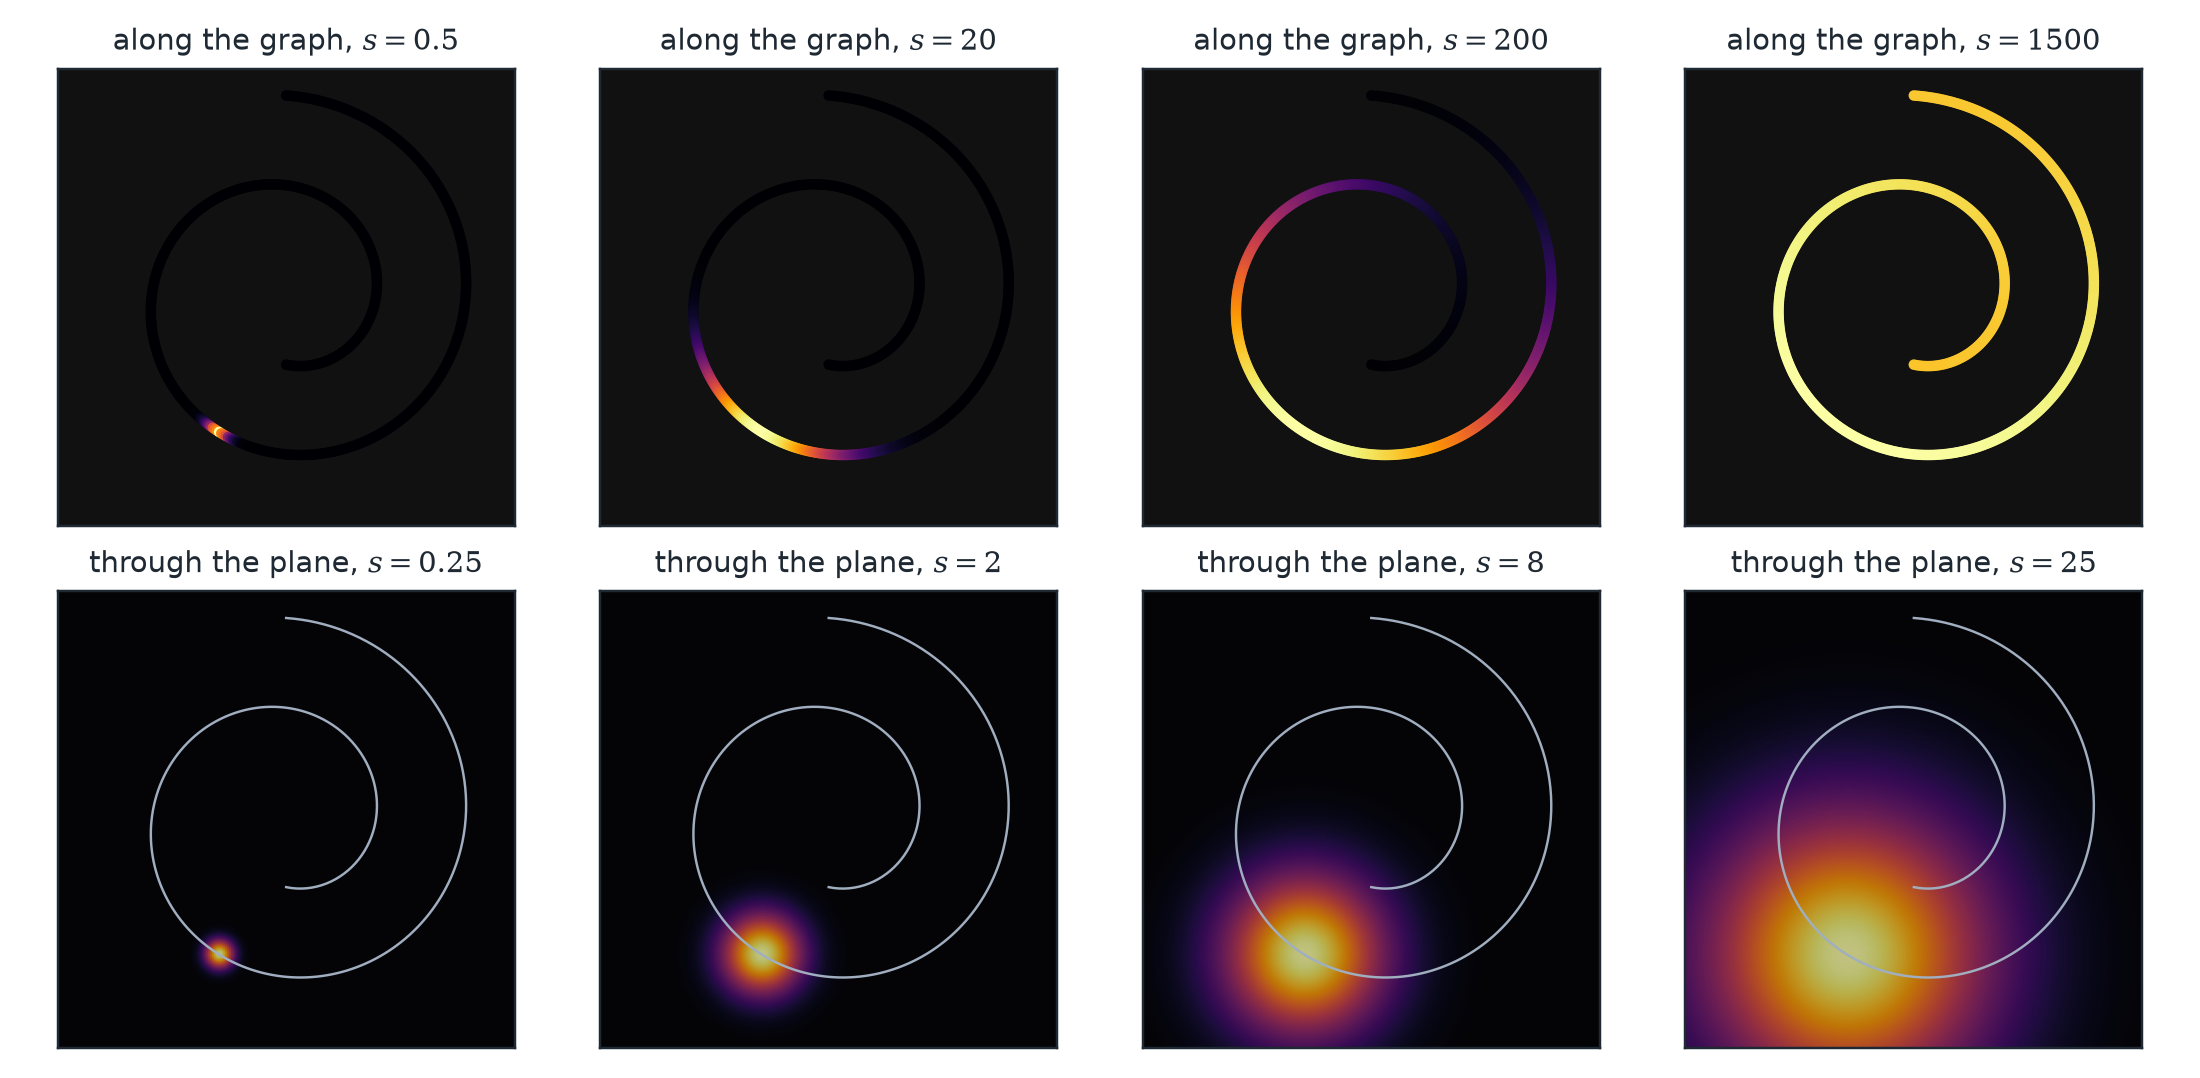
\includegraphics[width=\textwidth]{figures/lap_heat.png}
\caption{Heat released at one point of a spiral, each panel scaled to its own maximum. \emph{Top:} diffusion on a $k$-NN graph, $\bm u(s)=e^{-sL}\bm u(0)$. Heat travels along the curve and warms the neighboring layer only by going the long way around. \emph{Bottom:} ordinary diffusion through the plane, $\propto e^{-\norm{\vx-\vx_0}^2/(4s)}$, jumps straight across the gap. The time values in the two rows are not comparable. Each eigenvector decays at rate $\lambda$, so smooth waves last longest: that is another reason the small eigenvalues describe the large-scale shape.}
\label{fig:heat}
\end{figure}

\begin{deeper}
\textbf{The continuous picture: heat on the manifold.} As $N\to\infty$ and $\sigma\to0$ at a suitable rate, a rescaled graph Laplacian with RBF weights
converges to the \textbf{Laplace--Beltrami operator} $\Delta_M$ of the manifold (Belkin \& Niyogi). Its eigenvectors approximate the eigenfunctions of
$\Delta_M$, the smoothest functions on $M$ where smoothness is measured \emph{along} $M$, not through the ambient $\R^d$. The weight
$e^{-\norm{\vx-\vx'}^2/\sigma^2}$ is, up to constants, the short-time \textbf{heat kernel}: how much heat placed at $\vx$ reaches $\vx'$ in a short time.
Because the graph only links nearby points, heat diffuses \emph{along the manifold}, never across the gap between two layers of a Swiss roll. Figure~\ref{fig:heat} shows this on a spiral.

\textbf{Non-uniform sampling.} If points are denser in some regions, those vertices have larger degree, and the limit is no longer pure $\Delta_M$.
It picks up a drift toward high density. Normalizing by $D$ (in $L_{\mathrm{rw}}$ and $L_{\mathrm{sym}}$) corrects part of this. Two extensions go further.
\textbf{Diffusion maps} (Coifman \& Lafon) renormalize the kernel by an estimate of the density, removing the drift and recovering $\Delta_M$.
\textbf{UMAP} (Section~\ref{sec:umap}) rescales distances around each point so the data look uniformly spread on the manifold, keeping the local
structure while modeling away the density.

\textbf{Isomap vs.\ Laplacian eigenmaps.} Isomap preserves \emph{all} pairwise geodesic distances (a global goal, a dense matrix, and the largest
eigenvalues). Laplacian eigenmaps only asks that graph neighbors stay close (a local goal, a sparse matrix, and the smallest eigenvalues). The local
goal is cheaper and more robust to short-circuit edges, but it does not promise faithful large-scale distances.
\end{deeper}

\subsection{UMAP: Uniform Manifold Approximation and Projection}\label{sec:umap}

UMAP is a state-of-the-art tool for one job in particular: \textbf{visualization and exploratory cluster analysis}, with $t=2$ or $3$.
It builds a weighted neighbor graph, as Laplacian eigenmaps does, but with two changes that drive everything else. Each point gets its \emph{own} bandwidth, and
the embedding comes from a nonconvex optimization solved by stochastic gradient descent, not from an eigendecomposition.

\begin{deeper}
\textbf{Reading the name skeptically.} UMAP is often described as mathematically rigorous because its paper motivates it with fuzzy set topology and simplicial
complexes. The lecture's view is that this is largely branding: none of that machinery runs in the algorithm, and in practice UMAP is
closest to \textbf{t-SNE} (per-point bandwidths in high dimensions, a heavy-tailed similarity in low dimensions, gradient descent on a divergence).
Judge it by the steps below, which are concrete.
\end{deeper}

\subsubsection*{Step 1: nearest neighbors}
For each $\vx_i$, let $N_i$ be its $k$ nearest neighbors under Euclidean distance, \emph{not} including $\vx_i$ itself.
Unlike the graph in Section~\ref{sec:laplacian}, this is not symmetrized yet, so $j\in N_i$ does not imply $i\in N_j$. Step 3 handles that.

\subsubsection*{Step 2: a local scale for each point}
Each point gets two numbers: $\rho_i$, the distance to its nearest neighbor, and a bandwidth $\sigma_i>0$ solving
\[
\rho_i=\min_{j\in N_i}\norm{\vx_i-\vx_j},\qquad
\sum_{j\in N_i}\exp\!\Big(-\frac{\max\big(0,\ \norm{\vx_i-\vx_j}-\rho_i\big)}{\sigma_i}\Big)=\log_2 k .
\]
The two questions circled in your notes have short answers.
\begin{itemize}[nosep]
\item \textbf{How is $\rho_i$ found?} Directly: sort the distances to $N_i$ and read off the smallest. More generally, the \textbf{local connectivity} hyperparameter
$\ell$ (default $1$) makes $\rho_i$ the distance to the $\ell$-th nearest neighbor, so $\ell$ neighbors get weight exactly $1$.
\item \textbf{How is $\sigma_i$ found?} By \textbf{binary search}, separately for each $i$. Write $g_j=\max(0,\norm{\vx_i-\vx_j}-\rho_i)$ for the gaps and
$f(\sigma)=\sum_{j\in N_i}e^{-g_j/\sigma}$. Each term with $g_j>0$ strictly increases in $\sigma$, and $f$ runs from $\#\{j:g_j=0\}$ as $\sigma\to0$ up to $k$
as $\sigma\to\infty$. So when at least one gap is positive and $\#\{j:g_j=0\}<\log_2k<k$, there is exactly one solution.
With $\ell=1$ and no ties, that needs $k\ge3$. (At $k=2$, $\log_22=1$ is only reached in the limit $\sigma\to0$.)
\end{itemize}

\textbf{What the tuning accomplishes.} It forces every point's outgoing weights to add up to the \emph{same} total, $\log_2k$, so every point has the same ``effective
number of neighbors,'' wherever it sits. A point in a dense region has neighbors at small distances, so a small $\sigma_i$ is enough. A point in a sparse region needs a
large $\sigma_i$ to reach its far-away neighbors. That is the difference from the single global $\sigma$ in Laplacian eigenmaps and kernel PCA.

\begin{figure}[htbp]
\centering
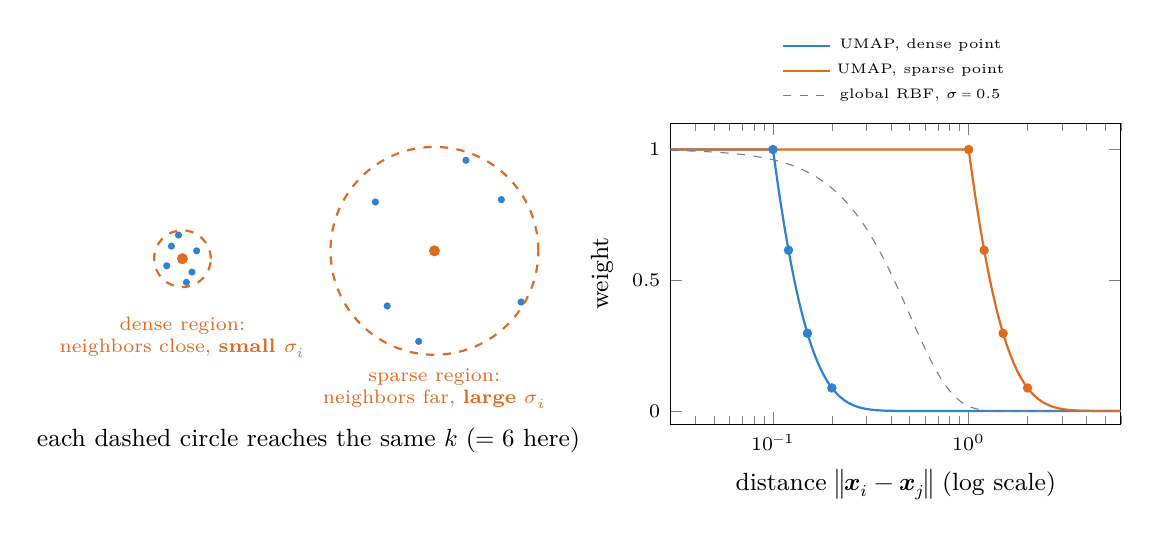
\begin{tikzpicture}[>=Stealth]
\begin{scope}
\foreach \p in {(0.18,0.1),(-0.14,0.16),(0.12,-0.17),(-0.2,-0.09),(-0.05,0.3),(0.05,-0.3)}
  \fill[dataC] \p circle (1.3pt);
\fill[accentC] (0,0) circle (2pt);
\draw[accentC,thick,dashed] (0,0) circle (0.36);
\node[font=\scriptsize,align=center,accentC] at (0,-1.0) {dense region:\\ neighbors close, \textbf{small $\sigma_i$}};
\foreach \p in {(3.2,0.1),(4.05,0.75),(4.3,-0.55),(2.6,-0.6),(2.45,0.72),(3.6,1.25),(3.0,-1.05)}
  \fill[dataC] \p circle (1.3pt);
\fill[accentC] (3.2,0.1) circle (2pt);
\draw[accentC,thick,dashed] (3.2,0.1) circle (1.32);
\node[font=\scriptsize,align=center,accentC] at (3.2,-1.65) {sparse region:\\ neighbors far, \textbf{large $\sigma_i$}};
\node[font=\small] at (1.6,-2.3) {each dashed circle reaches the same $k$ ($=6$ here)};
\end{scope}
\begin{scope}[xshift=6.2cm,yshift=-2.1cm]
\begin{axis}[width=7.3cm,height=5.4cm,xmode=log,xmin=0.03,xmax=6,ymin=-0.05,ymax=1.1,
  xlabel={distance $\norm{\vx_i-\vx_j}$ (log scale)},ylabel={weight},
  tick label style={font=\scriptsize},label style={font=\small},
  legend style={font=\tiny,at={(0.5,1.03)},anchor=south,draw=none,fill=none}]
\addplot[dataC,thick,domain=0.03:6,samples=300]{exp(-max(0,x-0.1)/0.0412)};
\addlegendentry{UMAP, dense point}
\addplot[accentC,thick,domain=0.03:6,samples=300]{exp(-max(0,x-1)/0.4116)};
\addlegendentry{UMAP, sparse point}
\addplot[ink!60,dashed,domain=0.03:6,samples=200]{exp(-x^2/0.25)};
\addlegendentry{global RBF, $\sigma=0.5$}
\addplot[only marks,mark=*,mark size=1.5pt,dataC,forget plot] coordinates {(0.10,1) (0.12,0.615) (0.15,0.297) (0.20,0.088)};
\addplot[only marks,mark=*,mark size=1.5pt,accentC,forget plot] coordinates {(1,1) (1.2,0.615) (1.5,0.297) (2,0.088)};
\end{axis}
\end{scope}
\end{tikzpicture}
\caption{\emph{Left:} the bandwidth adapts to local density (your sketch). \emph{Right:} the weight $\widetilde w_{ij}$ is flat at $1$ up to $\rho_i$ and then decays exponentially.
Dots are the neighbors in Example~\ref{ex:umapsigma}. On a log axis, the two UMAP curves are the same shape shifted, while one global RBF gives the dense point high weights and the sparse point almost none.}
\label{fig:umapsigma}
\end{figure}

\begin{example}{A dense point and a sparse point}{umapsigma}
Take $k=4$, so the target is $\log_24=2$. A dense point has neighbors at distances $0.10,0.12,0.15,0.20$; a sparse point has the same pattern ten times farther out.
Solving numerically gives $\sigma_i=0.0412$ and $\sigma_i=0.4116$:
\begin{center}
\small
\renewcommand{\arraystretch}{1.25}
\begin{tabular}{lcccc|c}
\toprule
& 1st & 2nd & 3rd & 4th & total\\
\midrule
UMAP, dense point & $1$ & $0.615$ & $0.297$ & $0.088$ & $2.00$\\
UMAP, sparse point & $1$ & $0.615$ & $0.297$ & $0.088$ & $2.00$\\
\midrule
Global RBF $e^{-d^2/\sigma^2}$, $\sigma=0.5$, dense point & $0.961$ & $0.944$ & $0.914$ & $0.852$ & $3.67$\\
Global RBF $e^{-d^2/\sigma^2}$, $\sigma=0.5$, sparse point & $0.018$ & $0.003$ & $0.000$ & $0.000$ & $0.02$\\
\bottomrule
\end{tabular}
\end{center}
Multiplying all of a point's neighbor distances by a constant multiplies $\rho_i$ and $\sigma_i$ by that constant and leaves the weights unchanged. UMAP's weights only see each point's
distances \emph{relative to its own scale}. This is the ``Uniform'' in the name: every region is treated as if it were sampled at the same density.
\end{example}

\subsubsection*{Step 3: compute and symmetrize the weights}
\[
\widetilde w_{ij}=\begin{cases}\exp\!\Big(-\dfrac{\max(0,\ \norm{\vx_i-\vx_j}-\rho_i)}{\sigma_i}\Big), & j\in N_i,\\[1ex] 0,&\text{otherwise,}\end{cases}
\qquad
w_{ij}=\widetilde w_{ij}+\widetilde w_{ji}-\widetilde w_{ij}\widetilde w_{ji}.
\]
If $\norm{\vx_i-\vx_j}\le\rho_i$ then $\widetilde w_{ij}=1$, so every point has weight $1$ to its nearest neighbor. No point is ever isolated, unlike the $\varepsilon$-ball graph in Figure~\ref{fig:epsknn}.
In general $\widetilde w_{ij}\ne\widetilde w_{ji}$, because $i$ and $j$ use different scales.

\begin{intuition}
\textbf{The symmetrization is ``probability of A or B.''} Read $\widetilde w_{ij}$ as the probability that $i$ proposes the edge to $j$. If the two proposals are treated as independent, the
chance that at least one happens is $1-(1-\widetilde w_{ij})(1-\widetilde w_{ji})$, which expands to the formula above. Therefore $w_{ij}\in[0,1]$, $w_{ij}=1$ if \emph{either} side is certain, and an edge
survives if either node wants it:
\begin{center}
\small
\renewcommand{\arraystretch}{1.2}
\begin{tabular}{cc|cc}
\toprule
$\widetilde w_{ij}$ & $\widetilde w_{ji}$ & $w_{ij}$ (union) & average, for comparison\\
\midrule
$1$ & $0$ & $1$ & $0.5$\\
$0.5$ & $0.5$ & $0.75$ & $0.5$\\
$0.2$ & $0$ & $0.2$ & $0.1$\\
\bottomrule
\end{tabular}
\end{center}
This matters for an outlier. Its nearest neighbor may not list it back, but the outlier's own proposal, $\widetilde w=1$, is enough to keep it attached at full strength.
\end{intuition}

\begin{figure}[htbp]
\centering
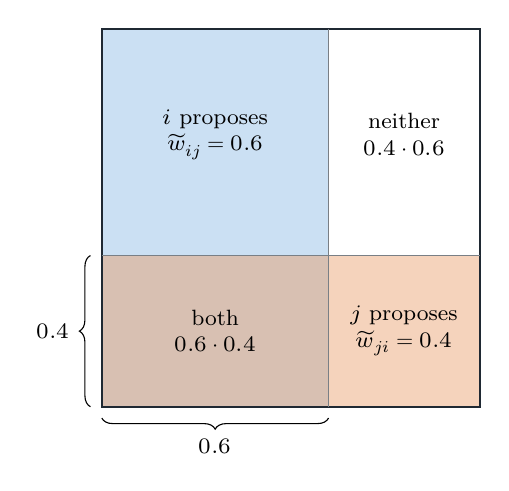
\begin{tikzpicture}[scale=4.8, every node/.style={font=\footnotesize}]
\fill[dataC!25] (0,0) rectangle (0.6,1);
\fill[accentC!30] (0,0) rectangle (1,0.4);
\fill[dataC!30!accentC!45] (0,0) rectangle (0.6,0.4);
\draw[thick,ink] (0,0) rectangle (1,1);
\draw[ink!60] (0.6,0) -- (0.6,1) (0,0.4) -- (1,0.4);
\node[align=center] at (0.3,0.72) {$i$ proposes\\$\widetilde w_{ij}=0.6$};
\node[align=center] at (0.8,0.2) {$j$ proposes\\$\widetilde w_{ji}=0.4$};
\node[align=center] at (0.3,0.2) {both\\$0.6\cdot0.4$};
\node[align=center] at (0.8,0.72) {neither\\$0.4\cdot0.6$};
\draw[decorate,decoration={brace,amplitude=4pt,mirror}] (0,-0.03) -- (0.6,-0.03) node[midway,below=4pt]{$0.6$};
\draw[decorate,decoration={brace,amplitude=4pt}] (-0.03,0) -- (-0.03,0.4) node[midway,left=4pt]{$0.4$};
\end{tikzpicture}
\caption{The symmetrization as an area. A random point in the unit square lands in the blue strip with probability $\widetilde w_{ij}$ and in the orange strip with probability $\widetilde w_{ji}$, independently. The edge exists if it lands in either: $0.6+0.4-0.6\cdot0.4=0.76$. Adding the two strips counts the corner twice, and the product removes the extra copy. Equivalently, $w_{ij}=1-(\text{white area})=1-0.4\cdot0.6$.}
\label{fig:umapunion}
\end{figure}

\begin{careful}
\textbf{A probability, not a probability distribution.} Each $w_{ij}$ is the success probability of \emph{one} yes/no event, ``is there an edge between $i$ and $j$?'' The $w_{ij}$ do not sum to $1$ over $j$ or over all pairs.
This is why the loss below is a sum of \emph{binary} comparisons, one per pair. (t-SNE normalizes its weights into one big distribution, which is a real difference.)
\end{careful}

\subsubsection*{Step 4: construct and optimize the low-dimensional representation}
For $\bm y_1,\dots,\bm y_N\in\R^t$, define the low-dimensional edge probability
\[
v_{ij}=\big(1+a\norm{\bm y_i-\bm y_j}^{2b}\big)^{-1},
\]
with $a,b>0$ set by a heuristic from the \texttt{min\_dist} hyperparameter. Then minimize, by SGD, the cross-entropy between the edge probabilities from the data and those from the embedding:
\[
C(\bm y_1,\dots,\bm y_N)=\sum_{i=1}^N\sum_{j\ne i}\Big[\underbrace{w_{ij}\log\frac{w_{ij}}{v_{ij}}}_{\text{attractive}}+\underbrace{(1-w_{ij})\log\frac{1-w_{ij}}{1-v_{ij}}}_{\text{repulsive}}\Big],
\]
with the convention $0\log0=0$. The $w_{ij}$ come from the data and are fixed; only the $v_{ij}$ depend on the $\bm y$'s.
The starting point is the \textbf{Laplacian eigenmaps} embedding (Section~\ref{sec:laplacian}), not a random one.

\begin{careful}
\textbf{``Cross-entropy'' is a loose name here.} Each bracket is the KL divergence between two yes/no distributions with probabilities $w_{ij}$ and $v_{ij}$. The true binary cross-entropy is $-w\log v-(1-w)\log(1-v)$.
They differ by the entropy of $w$, which does not depend on the $\bm y$'s, so the minimizer is the same. This also shows what each pair wants: a KL divergence is $0$ exactly when $v_{ij}=w_{ij}$.
\end{careful}

\begin{intuition}
\textbf{Two forces.} Take $a=b=1$ and $d=\norm{\bm y_i-\bm y_j}$, so $v=1/(1+d^2)$. Dropping constants, one pair contributes
\[
w\log(1+d^2)+(1-w)\log\!\Big(1+\frac1{d^2}\Big),\qquad
\nabla_{\bm y_i}=2(\bm y_i-\bm y_j)\Big[\frac{w}{1+d^2}-\frac{1-w}{d^2(1+d^2)}\Big].
\]
\begin{itemize}[nosep,leftmargin=*]
\item The $w$ term grows with $d$, so a gradient step \textbf{pulls} the pair together. It only acts where $w_{ij}>0$: on the order of $k$ terms per point.
\item The $1-w$ term blows up as $d\to0$ and fades as $d$ grows, so it \textbf{pushes} the pair apart. It acts on the order of $N-k$ terms per point.
\item The bracket vanishes at $d^2=(1-w)/w$, which is exactly $v=w$. For a true non-neighbor ($w=0$), the push never stops, but it gets weak quickly.
\end{itemize}
\textbf{Where the randomness comes from.} All the repulsive terms would cost $O(N^2)$ per pass. So SGD samples: for each attractive edge, it draws only a few random points (\texttt{negative\_sample\_rate}, default $5$)
as stand-ins for the whole repulsive sum. This keeps a pass near $O(Nk)$, but it makes the output depend on the random seed.
\end{intuition}

\begin{figure}[htbp]
\centering
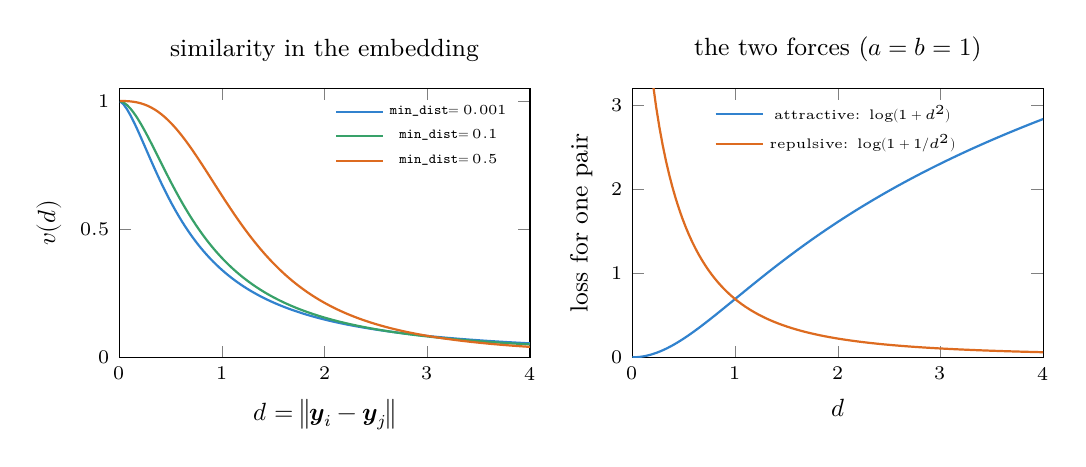
\begin{tikzpicture}
\begin{axis}[name=A,width=6.8cm,height=5cm,xmin=0,xmax=4,ymin=0,ymax=1.05,xlabel={$d=\norm{\bm y_i-\bm y_j}$},ylabel={$v(d)$},
  title={\small similarity in the embedding},tick label style={font=\scriptsize},label style={font=\small},
  legend style={font=\tiny,draw=none,fill=none,at={(0.98,0.98)},anchor=north east}]
\addplot[dataC,thick,domain=0.01:4,samples=120]{1/(1+1.929*x^(2*0.792))}; \addlegendentry{\texttt{min\_dist}$=0.001$}
\addplot[accentD,thick,domain=0.01:4,samples=120]{1/(1+1.577*x^(2*0.895))}; \addlegendentry{\texttt{min\_dist}$=0.1$}
\addplot[accentC,thick,domain=0.01:4,samples=120]{1/(1+0.583*x^(2*1.334))}; \addlegendentry{\texttt{min\_dist}$=0.5$}
\end{axis}
\begin{axis}[at={(A.east)},anchor=west,xshift=1.3cm,width=6.8cm,height=5cm,xmin=0,xmax=4,ymin=0,ymax=3.2,xlabel={$d$},ylabel={loss for one pair},
  title={\small the two forces ($a=b=1$)},tick label style={font=\scriptsize},label style={font=\small},
  legend style={font=\tiny,draw=none,fill=none,at={(0.5,0.98)},anchor=north}]
\addplot[dataC,thick,domain=0:4,samples=120]{ln(1+x^2)}; \addlegendentry{attractive: $\log(1+d^2)$}
\addplot[accentC,thick,domain=0.2:4,samples=120]{ln(1+1/x^2)}; \addlegendentry{repulsive: $\log(1+1/d^2)$}
\end{axis}
\end{tikzpicture}
\caption{\emph{Left:} $a,b$ fitted for three \texttt{min\_dist} values: $(a,b)=(1.93,0.79)$, $(1.58,0.90)$ and $(0.58,1.33)$. A larger \texttt{min\_dist} keeps $v$ high out to a larger distance, so points can sit farther apart and still count as close, which spreads clusters out.
\emph{Right:} attraction rises with distance, and repulsion dominates at short range, which stops points from landing on top of each other.}
\label{fig:umapforces}
\end{figure}

\begin{figure}[htbp]
\centering
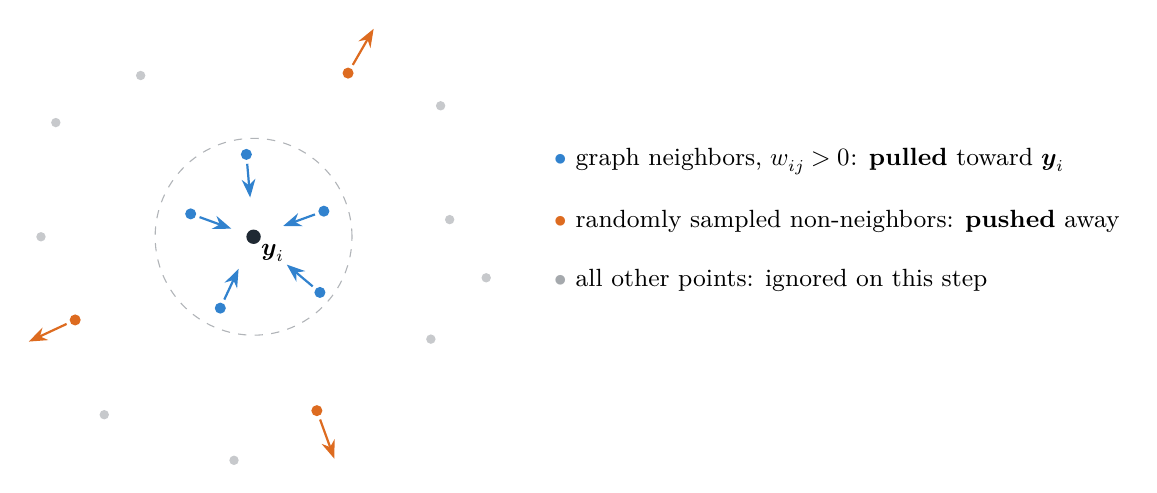
\begin{tikzpicture}[>=Stealth,scale=1.0]
\draw[dashed,ink!35] (0,0) circle (1.25);
\foreach \a/\r in {20/0.95,95/1.05,160/0.85,245/1.0,320/1.1} {\fill[dataC] (\a:\r) circle (2pt); \draw[->,thick,dataC] (\a:{\r-0.12}) -- (\a:{\r-0.55});}
\foreach \a/\r in {60/2.4,205/2.5,290/2.35} {\fill[accentC] (\a:\r) circle (2pt); \draw[->,thick,accentC] (\a:{\r+0.12}) -- (\a:{\r+0.65});}
\foreach \a/\r in {5/2.5,35/2.9,125/2.5,150/2.9,180/2.7,230/2.95,265/2.85,330/2.6,350/3.0} \fill[ink!25] (\a:\r) circle (1.7pt);
\fill[ink] (0,0) circle (2.6pt); \node[font=\small,below right=-1pt] at (0,0) {$\bm y_i$};
\node[font=\small,anchor=west,align=left] at (3.7,0.95) {\textcolor{dataC}{$\bullet$} graph neighbors, $w_{ij}>0$: \textbf{pulled} toward $\bm y_i$};
\node[font=\small,anchor=west,align=left] at (3.7,0.2) {\textcolor{accentC}{$\bullet$} randomly sampled non-neighbors: \textbf{pushed} away};
\node[font=\small,anchor=west,align=left] at (3.7,-0.55) {\textcolor{ink!40}{$\bullet$} all other points: ignored on this step};
\end{tikzpicture}
\caption{One SGD step around $\bm y_i$. Only about $k$ neighbors and a few samples act, not all $N$ points. Each pair is moved along the line joining the two points.}
\label{fig:umapstep}
\end{figure}

\begin{algorithm}{UMAP}{umap}
Input: $\vx_1,\dots,\vx_N\in\R^d$; hyperparameters $t$, $k$, $\ell$, \texttt{min\_dist} and the SGD settings.
\begin{enumerate}[nosep]
\item Find the $k$ nearest neighbors $N_i$ of each $\vx_i$ (excluding $\vx_i$).
\item For each $i$, set $\rho_i$ from the $\ell$-th nearest neighbor, and find $\sigma_i$ by binary search so that the weights sum to $\log_2k$.
\item Compute $\widetilde w_{ij}$, then $w_{ij}=\widetilde w_{ij}+\widetilde w_{ji}-\widetilde w_{ij}\widetilde w_{ji}$.
\item Initialize $\bm y_1,\dots,\bm y_N$ with Laplacian eigenmaps, then minimize $C$ by SGD: attract along edges, repel from randomly sampled points.
\end{enumerate}
\end{algorithm}

\begin{center}
\renewcommand{\arraystretch}{1.3}
\small
\begin{tabular}{>{\raggedright\arraybackslash}p{3cm}>{\raggedright\arraybackslash}p{3.7cm}>{\raggedright\arraybackslash}p{6.6cm}}
\toprule
Group & Hyperparameter & What it controls\\
\midrule
Output & $t$ & dimension of the $\bm y_i$; almost always $2$ or $3$\\
Neighborhood & $k$ & the main tuning lever: small $k$ favors fine local detail, large $k$ favors broader structure\\
 & local connectivity $\ell$ & how many neighbors get weight $1$, through $\rho_i$ (default $1$)\\
Embedding shape & \texttt{min\_dist} & $a,b$, and so how tightly points may pack; moderate visual effect\\
SGD & learning rate, epochs, negative samples & usually left at their defaults\\
\bottomrule
\end{tabular}
\end{center}

\subsubsection*{Watching it run, and turning the knobs}

These two figures run UMAP on real data: $1797$ handwritten digit images of $8\times8$ pixels, so $d=64$. Color marks the true digit. UMAP never sees these labels, so any separation it shows comes from pixel neighborhoods alone.

\begin{figure}[htbp]
\centering
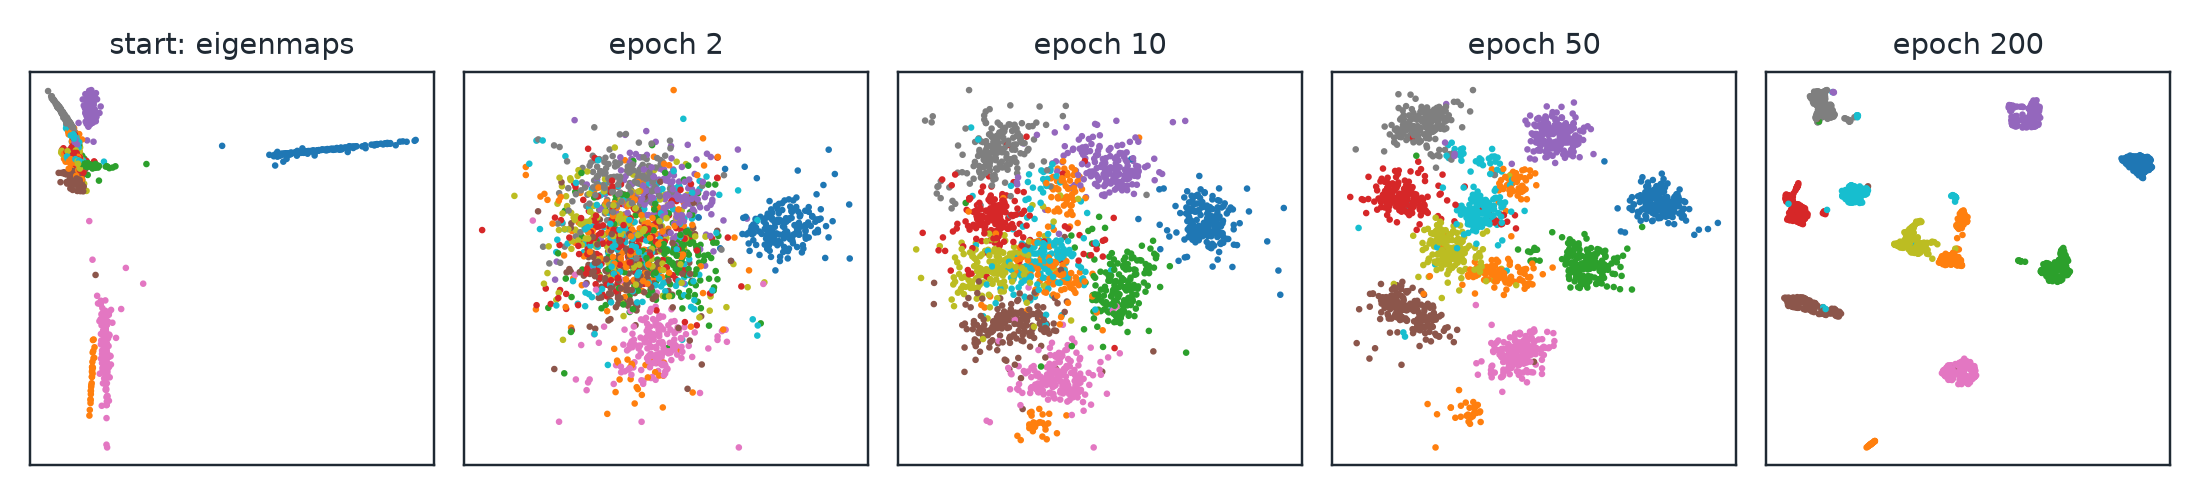
\includegraphics[width=\textwidth]{figures/umap_snapshots.png}
\caption{The optimization, from the Laplacian eigenmaps start to the end of SGD ($k=15$). Each panel has its own axis scale. Early steps are large and mix the points. The attractive and repulsive forces then pull the classes into separate clusters, which keep tightening.}
\label{fig:umapsnap}
\end{figure}

\begin{figure}[htbp]
\centering
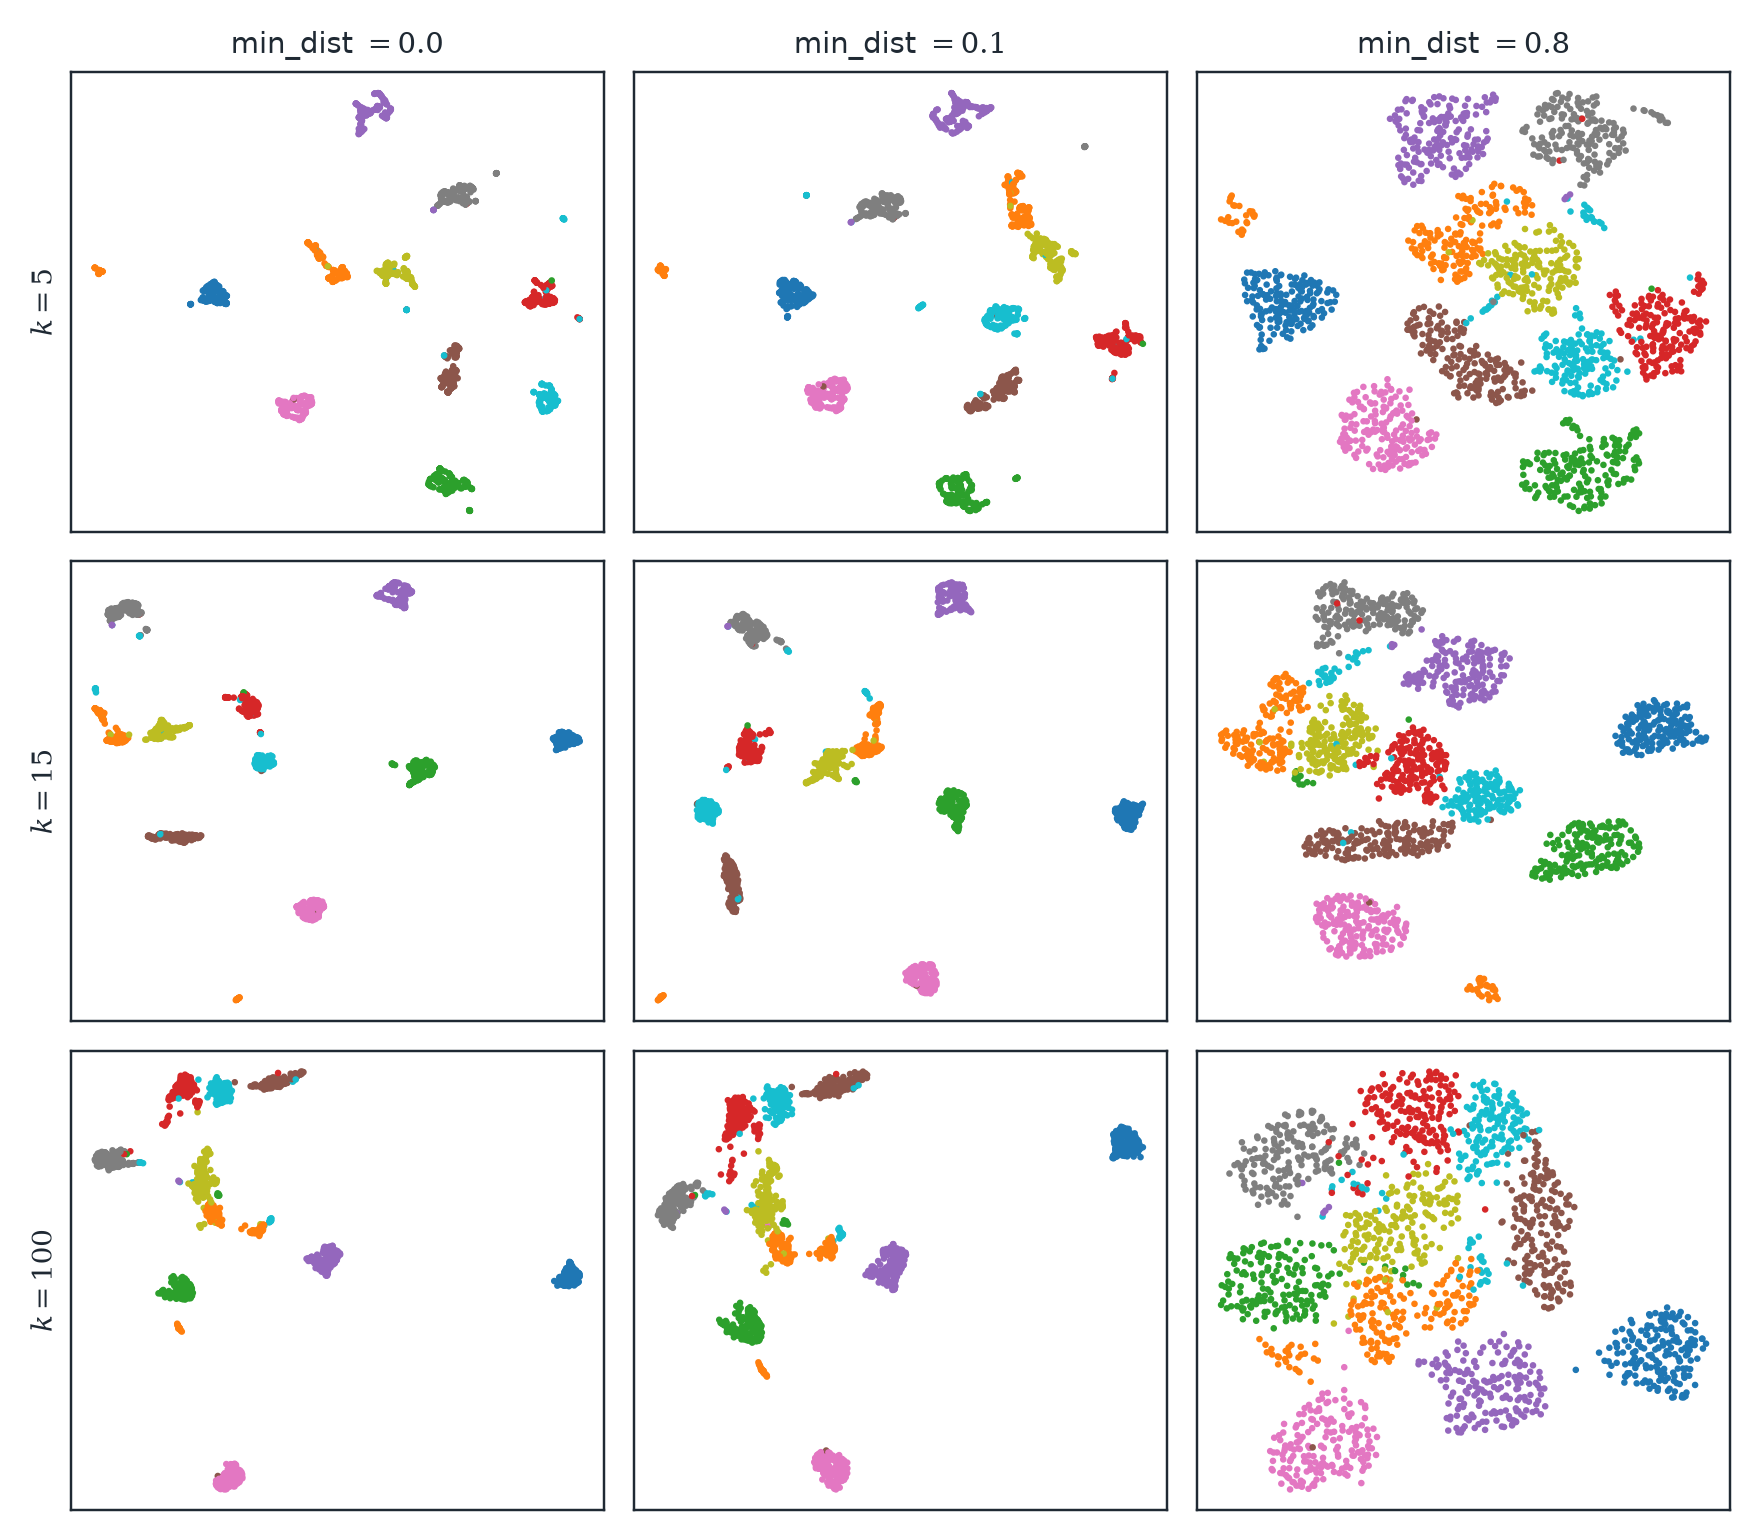
\includegraphics[width=0.82\textwidth]{figures/umap_grid.png}
\caption{The two main knobs on the same data. Reading across a row: a larger \texttt{min\_dist} spreads each cluster without much changing which points are together. Reading down a column: a small $k$ gives more stray fragments, and a large $k$ gives more connected, broader structure. Positions of clusters change between panels, so they should not be over-read.}
\label{fig:umapgrid}
\end{figure}

\FloatBarrier
\subsubsection*{Isomap, Laplacian eigenmaps and UMAP on the same data}

\begin{figure}[htbp]
\centering
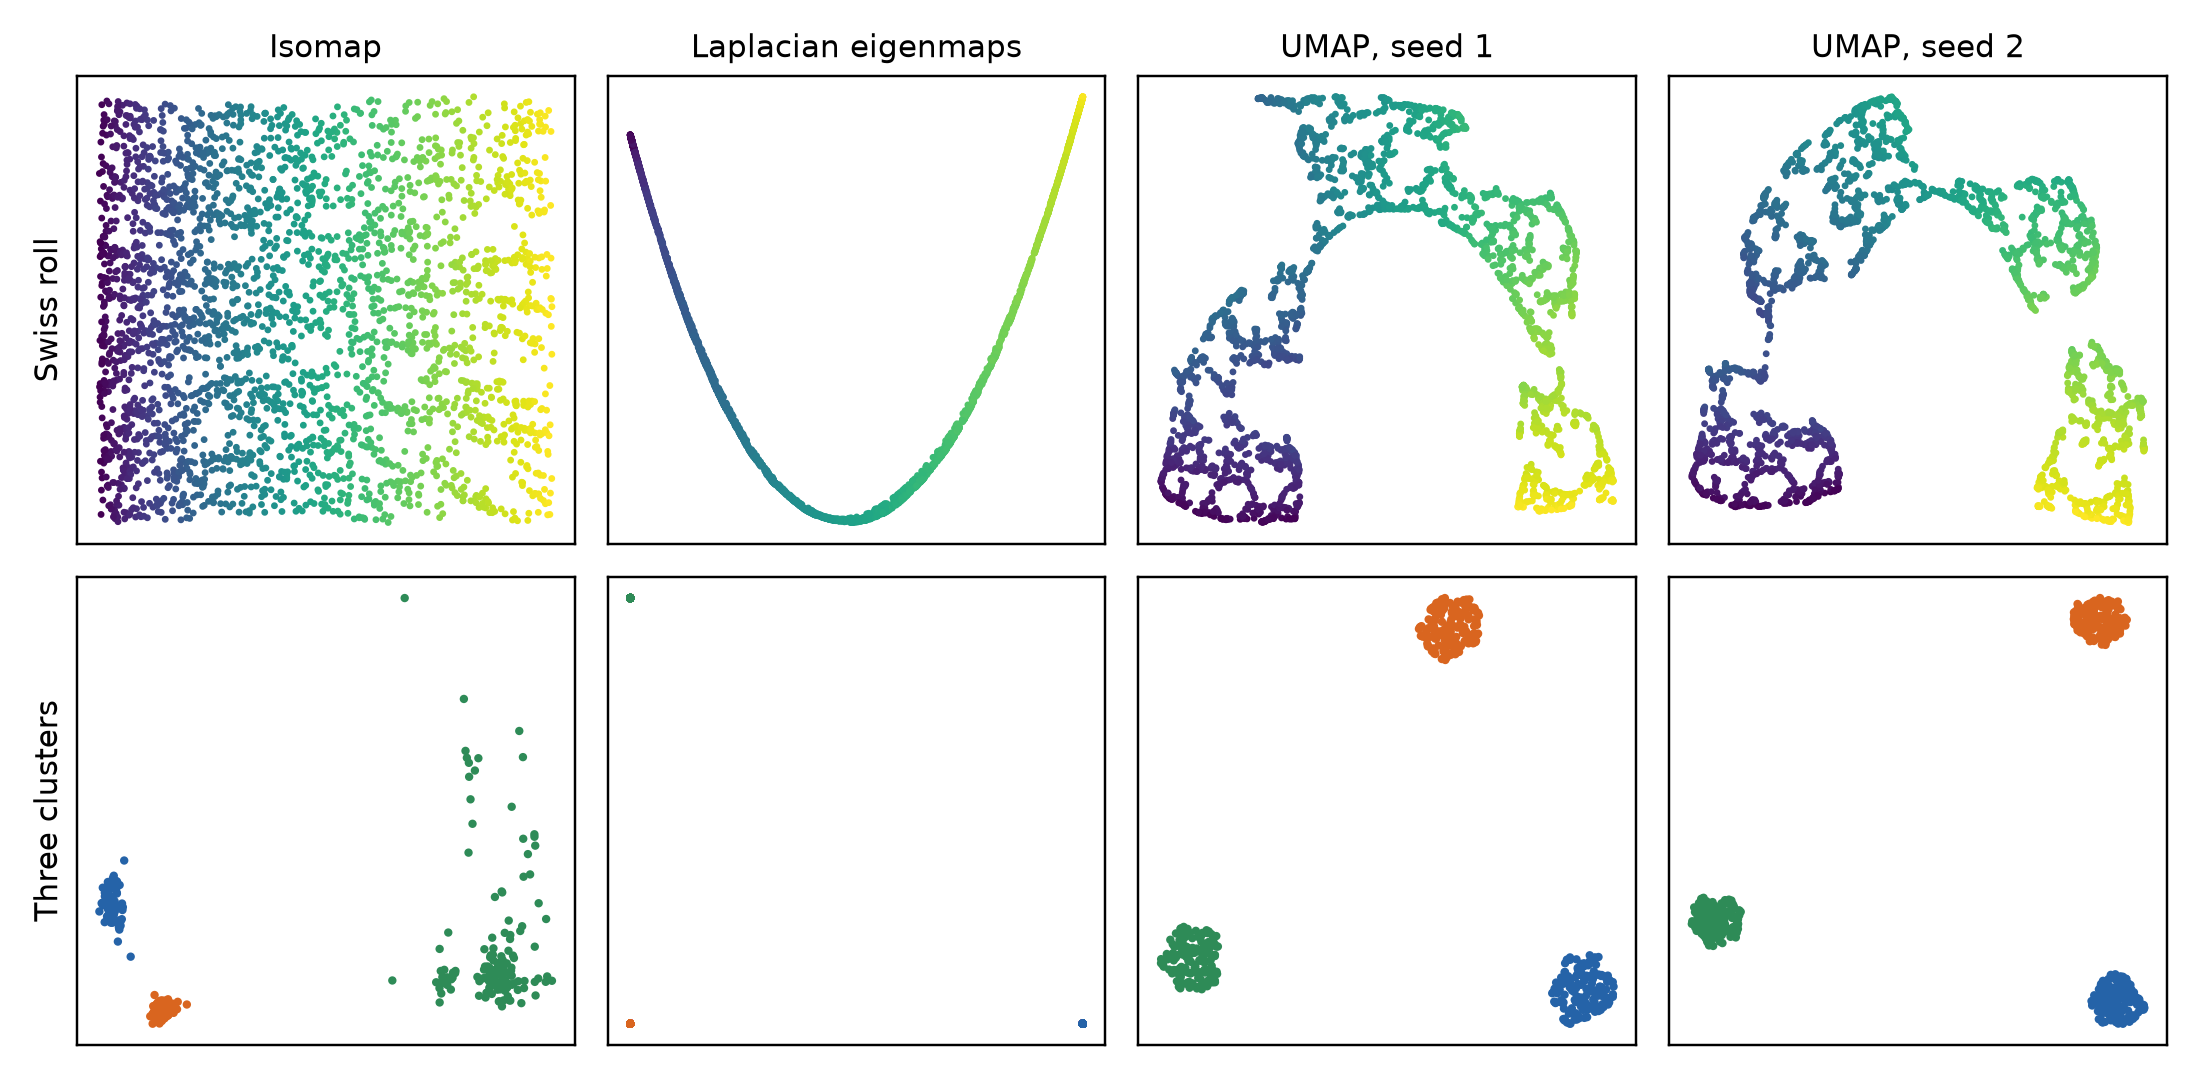
\includegraphics[width=\textwidth]{figures/umap_compare.png}
\caption{Real runs with $k=15$. \emph{Top:} a Swiss roll with $3000$ points, colored by position along the roll. \emph{Bottom:} three Gaussian clusters of $150$ points in $\R^{10}$ with centers about $6$ (blue--orange) and $40$ (blue--green) apart.
Blue and orange have standard deviation $0.5$; green is much sparser, at $3$. The Isomap and eigenmaps $k$-NN graphs fall apart on the bottom row, so the software's Isomap stitches the pieces together, and eigenmaps collapses each piece to a dot.}
\label{fig:umapcompare}
\end{figure}

\begin{center}
\renewcommand{\arraystretch}{1.25}
\small
\begin{tabular}{lcc}
\toprule
Bottom row of Figure~\ref{fig:umapcompare} & between-cluster distance ratio, $\dfrac{\text{blue--green}}{\text{blue--orange}}$ & cluster spread, green $/$ blue\\
\midrule
Original data & $6.63$ & $6.1$\\
Isomap & $4.46$ & $5.6$\\
UMAP, seed 1 & $1.11$ & $0.95$\\
UMAP, seed 2 & $1.05$ & $0.97$\\
\bottomrule
\end{tabular}
\end{center}

\textbf{What the figure shows.} Isomap flattens the roll into a rectangle and roughly keeps the sizes and spacing of the clusters. Laplacian eigenmaps bends the roll into a smooth arch, a clean ordering along the roll with the width direction lost, and on the clusters
it does exactly what Section~\ref{sec:laplacian} predicted for a disconnected graph. UMAP separates the clusters perfectly, but the far-apart cluster looks no farther away than the near one, the sparse cluster looks as tight as the dense ones, and the
roll breaks into local clumps that differ from seed to seed. The table puts numbers on this: UMAP nearly erases both the distance ratio and the density difference.

\begin{center}
\renewcommand{\arraystretch}{1.3}
\small
\begin{tabular}{>{\raggedright\arraybackslash}p{2.9cm}>{\raggedright\arraybackslash}p{3.3cm}>{\raggedright\arraybackslash}p{3.3cm}>{\raggedright\arraybackslash}p{3.7cm}}
\toprule
& Isomap & Laplacian eigenmaps & UMAP\\
\midrule
Preserves & global geodesic distances & smooth coordinates; a blend of local and high-level structure & local connectivity\\
Embedding distances & quantitatively meaningful (if assumptions hold) & only loosely & \textbf{not meaningful} between clusters\\
Uneven sampling & sensitive & partly corrected by $D$ & robust (adaptive $\sigma_i$)\\
Solved by & eigendecomposition & sparse eigendecomposition & nonconvex SGD\\
Same output every run? & yes & yes & \textbf{no}\\
Best for & faithful maps of a manifold & smooth coordinates, spectral analysis & seeing clusters\\
\bottomrule
\end{tabular}
\end{center}

\begin{careful}
\textbf{How not to read a UMAP plot.}
\begin{itemize}[nosep,leftmargin=*]
\item \textbf{Gaps and cluster sizes carry little information.} Neither the distance between two clusters nor how spread out one looks should be read as a measurement. A tight cluster is not necessarily a dense one.
\item \textbf{Different seeds can give different pictures.} SGD sampling is the source your notes name; the approximate nearest-neighbor search that fast implementations use adds a little more. Rerun with a few seeds before trusting a feature of the plot.
\item \textbf{``Destroys global structure'' is a tendency.} The objective has no term for far-apart pairs beyond ``keep them apart,'' so nothing protects large-scale geometry. The large-scale layout you do see is inherited largely from the Laplacian eigenmaps start (Kobak \& Linderman, 2021), which is one reason initialization matters.
On the t-SNE contrast: its original form started at random, though current software commonly starts from PCA.
\end{itemize}
\end{careful}

\subsubsection*{Choosing $k$: too small, about right, too large}

All three methods start from a neighbor graph, so all three inherit its problems (Figure~\ref{fig:keffect}). No single value is right for every dataset, and it is worth trying several and seeing which features persist.

\begin{figure}[htbp]
\centering
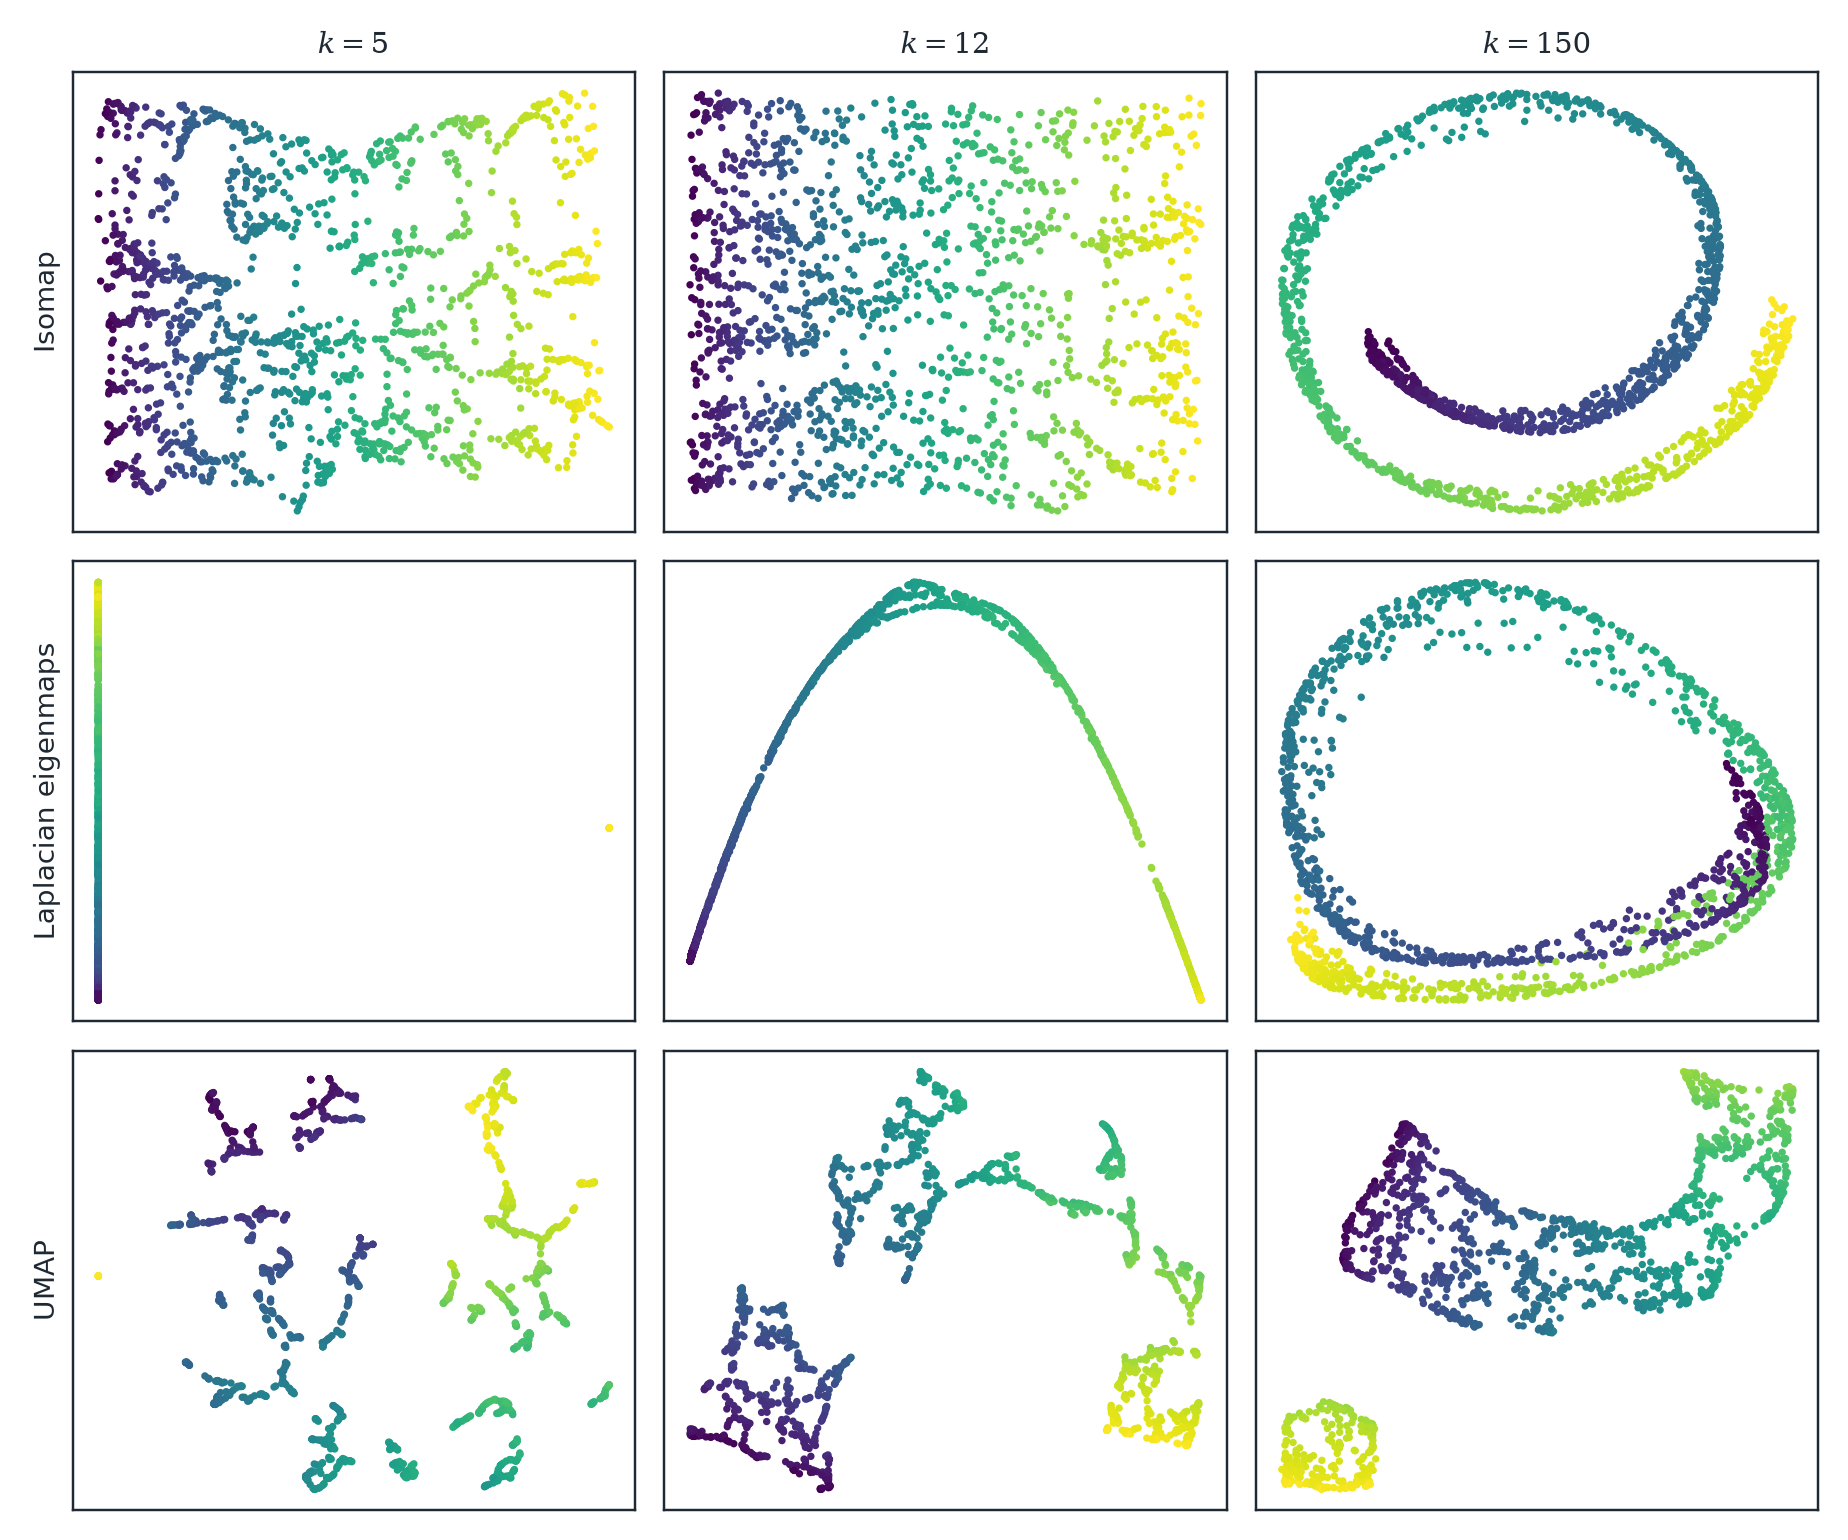
\includegraphics[width=0.86\textwidth]{figures/k_effect.png}
\caption{A $1500$-point Swiss roll at three values of $k$; the graph is connected in all of them. $k=5$: Isomap's rectangle is full of holes, because graph paths are jagged; a few barely attached points take over a coordinate in Laplacian eigenmaps; UMAP breaks into fragments. $k=12$: Isomap gives a rectangle and eigenmaps the arch. $k=150$ ($10\%$ of the data): neighborhoods reach across layers, so Isomap and eigenmaps no longer unroll it and both wrap it around on itself, while UMAP keeps much of the local order but detaches the far end of the roll.}
\label{fig:keffect}
\end{figure}

\clearpage
% ==================================================================
\section{Autoencoders and Self-Supervised Learning}\label{sec:autoencoder}
% ==================================================================

\subsection{The missing way back}

Isomap, Laplacian eigenmaps and UMAP have all been a \textbf{one-way trip}: data in $\R^d$ go to coordinates in $\R^t$ with $t<d$, and the method provides no map back. With a way back, we could work in the low-dimensional \textbf{latent space} and return to the original data space, including to create new data.

\textbf{The idea.} Section~\ref{sec:manifold} pictured the data as $\vx=\psi(\bm y)$ for a map $\psi:\R^t\to\R^d$ onto a manifold. Model both directions directly, with neural networks:
\[
\text{encoder } E_\theta:\R^d\to\R^t\ \ (\text{plays the role of }\psi^{-1}),\qquad \text{decoder } D_\phi:\R^t\to\R^d\ \ (\text{plays the role of }\psi).
\]

\begin{figure}[htbp]
\centering
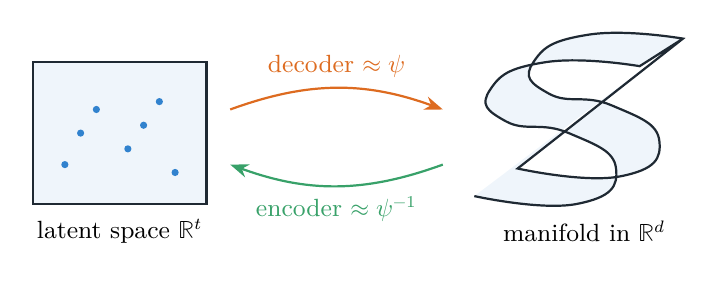
\begin{tikzpicture}[>=Stealth]
\draw[thick,ink,fill=dataC!8] (0,0) rectangle (2.2,1.8);
\foreach \p in {(0.4,0.5),(0.8,1.2),(1.2,0.7),(1.6,1.3),(1.8,0.4),(0.6,0.9),(1.4,1.0)} \fill[dataC] \p circle (1.3pt);
\node[font=\small] at (1.1,-0.35) {latent space $\R^t$};
\draw[->,thick,accentC] (2.5,1.2) to[bend left=20] node[above,font=\small]{decoder $\approx\psi$} (5.2,1.2);
\draw[<-,thick,accentD] (2.5,0.5) to[bend right=20] node[below,font=\small]{encoder $\approx\psi^{-1}$} (5.2,0.5);
\draw[thick,ink,fill=dataC!8] plot[smooth,tension=0.9] coordinates {(5.6,0.1) (6.9,0.0) (7.4,0.45) (6.8,0.9) (6.0,1.05) (5.8,1.45) (6.5,1.8) (7.7,1.75)} -- ++(0.55,0.35) plot[smooth,tension=0.9] coordinates {(8.25,2.1) (7.05,2.15) (6.35,1.8) (6.55,1.4) (7.35,1.25) (7.95,0.8) (7.45,0.35) (6.15,0.45)} -- cycle;
\node[font=\small] at (7.0,-0.35) {manifold in $\R^d$};
\end{tikzpicture}
\caption{The round trip. Earlier methods only compute the arrow to the left, and only at the training points.}
\label{fig:aeroundtrip}
\end{figure}

\begin{careful}
\textbf{``$\psi^{-1}$'' is shorthand.} A map from $\R^t$ to $\R^d$ with $t<d$ has no true inverse on all of $\R^d$; at best it inverts on the manifold. An encoder is defined at \emph{every} $\vx\in\R^d$, including points off the manifold, where it acts more like a projection. So $D\circ E$ is at best the identity on the manifold, and $E\circ D$ is the identity on the latent points the decoder actually uses.
\end{careful}

\subsection{Neural networks in one page}

A two-layer network is just a composition of affine maps and nonlinearities:
\[
f(\vx)=\sigma_2\Big(A^{(2)}\,\sigma_1\big(A^{(1)}\vx+\bm b^{(1)}\big)+\bm b^{(2)}\Big).
\]
Its \textbf{parameters} are the matrices $A^{(1)},A^{(2)}$ and vectors $\bm b^{(1)},\bm b^{(2)}$. The superscripts label layers, not powers. The \textbf{activations} $\sigma_1,\sigma_2$ apply entry by entry and are fixed in advance (for example ReLU, $\sigma(s)=\max(0,s)$, or the identity at the output).

\begin{figure}[htbp]
\centering
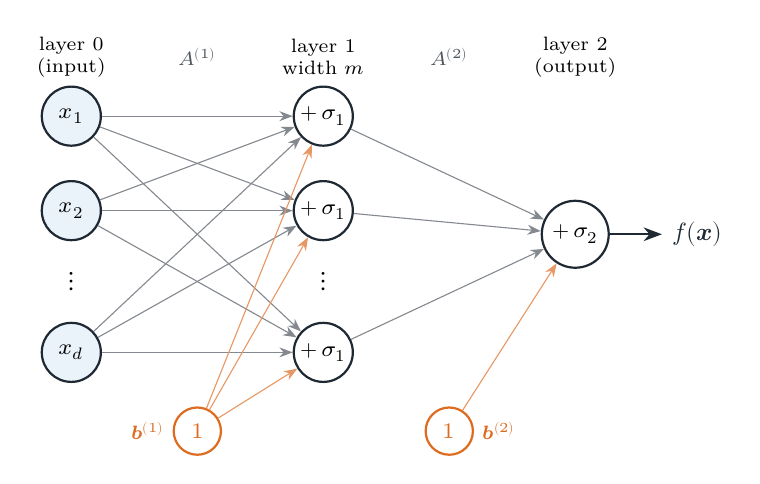
\begin{tikzpicture}[>=Stealth,
  nn/.style={circle,draw=ink,thick,minimum size=7.5mm,inner sep=0pt,font=\footnotesize},
  bias/.style={circle,draw=accentC,thick,minimum size=6mm,inner sep=0pt,font=\footnotesize,accentC},
  ar/.style={->,ink!55,thin}]
\foreach \i/\y/\l in {1/3.0/x_1,2/1.8/x_2,3/0.0/x_d} \node[nn,fill=dataC!10] (x\i) at (0,\y) {$\l$};
\node at (0,0.9) {$\vdots$};
\foreach \i/\y in {1/3.0,2/1.8,3/0.0} \node[nn] (h\i) at (3.2,\y) {$+\,\sigma_1$};
\node at (3.2,0.9) {$\vdots$};
\node[nn,minimum size=8.5mm] (o) at (6.4,1.5) {$+\,\sigma_2$};
\node[bias] (b1) at (1.6,-1.0) {$1$};
\node[bias] (b2) at (4.8,-1.0) {$1$};
\foreach \i in {1,2,3} \foreach \j in {1,2,3} \draw[ar] (x\i) -- (h\j);
\foreach \j in {1,2,3} \draw[ar] (h\j) -- (o);
\foreach \j in {1,2,3} \draw[->,accentC!70,thin] (b1) -- (h\j);
\draw[->,accentC!70,thin] (b2) -- (o);
\draw[->,thick,ink] (o) -- ++(1.1,0) node[right,font=\small]{$f(\vx)$};
\node[font=\scriptsize,align=center] at (0,3.75) {layer 0\\(input)};
\node[font=\scriptsize,align=center] at (3.2,3.75) {layer 1\\ width $m$};
\node[font=\scriptsize,align=center] at (6.4,3.75) {layer 2\\(output)};
\node[font=\scriptsize,ink!80] at (1.6,3.75) {$A^{(1)}$};
\node[font=\scriptsize,ink!80] at (4.8,3.75) {$A^{(2)}$};
\node[font=\scriptsize,accentC,left] at (1.3,-1.0) {$\bm b^{(1)}$};
\node[font=\scriptsize,accentC,right] at (5.1,-1.0) {$\bm b^{(2)}$};
\end{tikzpicture}
\caption{The network from your notes. Each node takes a weighted sum of its inputs plus a constant, then applies its activation. Each edge weight is one entry of $A^{(\cdot)}$, and the edges from a ``$1$'' node are the entries of $\bm b^{(\cdot)}$.}
\label{fig:nn}
\end{figure}

\begin{center}
\renewcommand{\arraystretch}{1.25}
\small
\begin{tabular}{llll}
\toprule
Object & Size & Meaning & Parameters\\
\midrule
$\vx$ & $\R^d$ & input (one data point) & \\
$A^{(1)},\ \bm b^{(1)}$ & $\R^{m\times d},\ \R^m$ & row $r$ of $A^{(1)}$: the edges into hidden node $r$ & $m(d+1)$\\
$A^{(2)},\ \bm b^{(2)}$ & $\R^{p\times m},\ \R^p$ & $p$ output nodes & $p(m+1)$\\
\bottomrule
\end{tabular}
\end{center}

\begin{careful}
\begin{itemize}[nosep,leftmargin=*]
\item \textbf{Input nodes are coordinates, not data points.} Layer 0 has $d$ nodes, the coordinates $x_1,\dots,x_d$ of a \emph{single} point. (Elsewhere in these notes $\vx_i$ is the $i$-th data point; the two uses of a subscript differ.) Your sketch labels the last node with $N$ or $n$, which would suggest a node per data point. It should be $d$.
\item \textbf{Vector or scalar output.} Your sketch ends in one output node, which makes $A^{(2)}$ a single row and $\bm b^{(2)}$ a single number. An autoencoder needs a vector output, hence the general $p$.
\item \textbf{Symbols reused.} $\sigma_1,\sigma_2$ here are activations, not UMAP's bandwidths $\sigma_i$. $A^{(\ell)}$ are weight matrices, not the affinity matrix $A$.
\end{itemize}
\end{careful}

\begin{example}{One forward pass}{forward}
Let $d=2$, $m=2$, $p=1$, $\sigma_1=$ ReLU, $\sigma_2=$ identity, with
$A^{(1)}=\begin{bmatrix}1&-1\\0&1\end{bmatrix}$, $\bm b^{(1)}=\begin{bmatrix}0\\-1\end{bmatrix}$, $A^{(2)}=\begin{bmatrix}2&3\end{bmatrix}$, $b^{(2)}=-1$, and $\vx=(1,2)\T$.
Then $A^{(1)}\vx+\bm b^{(1)}=(-1,\,1)\T$, ReLU gives $(0,1)\T$, and $f(\vx)=2\cdot0+3\cdot1-1=2$.
\textbf{Why the nonlinearity is essential:} without it, $f$ is an affine map of an affine map, which is just one affine map, however many layers you stack.
\end{example}

\subsection{The autoencoder}

An autoencoder composes the two networks and trains them \emph{together}, as one network, to reproduce its own input:
\[
\min_{\theta,\phi}\ \sum_{i=1}^N\norm{\vx_i-D_\phi\big(E_\theta(\vx_i)\big)}^2,\qquad\text{latent code }\bm y_i=E_\theta(\vx_i)\in\R^t .
\]
The minimization uses stochastic gradient descent, with gradients from the chain rule (backpropagation).

\begin{figure}[htbp]
\centering
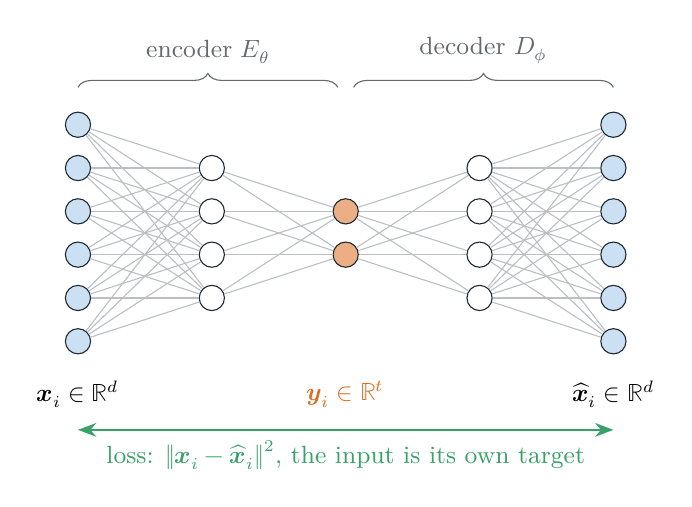
\begin{tikzpicture}[>=Stealth,nd/.style={circle,draw=ink,fill=#1,inner sep=0pt,minimum size=3.2mm}]
\def\lay#1#2#3#4{\foreach \k in {1,...,#2} \node[nd=#4] (#3\k) at (#1,{(#2+1)/2*0.55-\k*0.55}) {};}
\lay{0}{6}{a}{dataC!25}\lay{1.7}{4}{b}{white}\lay{3.4}{2}{c}{accentC!55}\lay{5.1}{4}{d}{white}\lay{6.8}{6}{e}{dataC!25}
\foreach \i in {1,...,6} \foreach \j in {1,...,4} \draw[ink!30,thin] (a\i)--(b\j);
\foreach \i in {1,...,4} \foreach \j in {1,2} \draw[ink!30,thin] (b\i)--(c\j);
\foreach \i in {1,2} \foreach \j in {1,...,4} \draw[ink!30,thin] (c\i)--(d\j);
\foreach \i in {1,...,4} \foreach \j in {1,...,6} \draw[ink!30,thin] (d\i)--(e\j);
\node[font=\small] at (0,-2.05) {$\vx_i\in\R^d$};
\node[font=\small,accentC] at (3.4,-2.05) {$\bm y_i\in\R^t$};
\node[font=\small] at (6.8,-2.05) {$\widehat{\vx}_i\in\R^d$};
\draw[decorate,decoration={brace,amplitude=5pt},ink!70] (0,1.85) -- (3.3,1.85) node[midway,above=5pt,font=\small]{encoder $E_\theta$};
\draw[decorate,decoration={brace,amplitude=5pt},ink!70] (3.5,1.85) -- (6.8,1.85) node[midway,above=5pt,font=\small]{decoder $D_\phi$};
\draw[<->,thick,accentD] (0,-2.5) -- (6.8,-2.5) node[midway,below,font=\small]{loss: $\norm{\vx_i-\widehat{\vx}_i}^2$, the input is its own target};
\end{tikzpicture}
\caption{Wide, then a narrow bottleneck of width $t$, then wide again.}
\label{fig:hourglass}
\end{figure}

\begin{intuition}
\textbf{Self-supervised: the data label themselves.} Supervised regression needs pairs (input, target). Here each $\vx_i$ is its own target, so an unsupervised problem is turned into ordinary supervised training with no external labels. The target alone would be trivial, since the identity map scores zero. The \textbf{bottleneck} is what makes the task meaningful: everything must pass through $t<d$ numbers, so the network has to find a compact description. This is Fact~\ref{kf:bottleneck} in nonlinear form.
\end{intuition}

\begin{proposition}{A linear autoencoder is PCA}{linae}
Take $E(\vx)=B\vx+\bm c$ and $D(\bm y)=A\bm y+\bm e$ with $A\in\R^{d\times t}$, $B\in\R^{t\times d}$ and no activations. Then the best possible reconstruction is PCA's: $\widehat{\vx}=\xbar+W_tW_t\T(\vx-\xbar)$, with $W_t$ the top $t$ loadings. The product $AB$ has the column space of $W_t$, but $A$ and $B$ individually need not be $W_t$.
\end{proposition}
\begin{proofsketch}
The reconstruction is $\widehat{\vx}=AB\vx+$ constant, where $AB$ has rank at most $t$ (a rank-$t$ bottleneck) and the free constant makes centering optimal. Minimizing $\Fro{HX-HX(AB)\T}^2$ over rank-$t$ matrices is Eckart--Young, so $AB=W_tW_t\T$ is optimal. For any invertible $G$, replacing $A,B$ by $AG,G^{-1}B$ leaves $AB$ unchanged, so the columns of $A$ need not be orthonormal or be the principal directions.
\end{proofsketch}

\begin{example}{The circle: where nonlinearity wins, and where it hits a wall}{aecircle}
Let the data be points $\vx=(\cos\alpha,\sin\alpha)\T$ spread evenly around the unit circle, with $t=1$.
\begin{itemize}[nosep]
\item \textbf{Linear ($=$ PCA):} each of the two directions has equal variance, so one direction always loses half of the total variance.
\item \textbf{Nonlinear:} $E(\vx)=\alpha$ and $D(\alpha)=(\cos\alpha,\sin\alpha)\T$ reconstruct perfectly with one number. This is the intrinsic dimension at work.
\item \textbf{The wall:} that $E$ must \emph{jump} somewhere (from just under $2\pi$ to $0$), and no continuous map from the circle to $\R$ can be one-to-one. Standard networks are continuous, so a real encoder can only approximate this: it reconstructs well except near one steep ``seam.'' This is the gluing problem of Figure~\ref{fig:glue} again, in the encoder.
\end{itemize}
\end{example}

\begin{figure}[htbp]
\centering
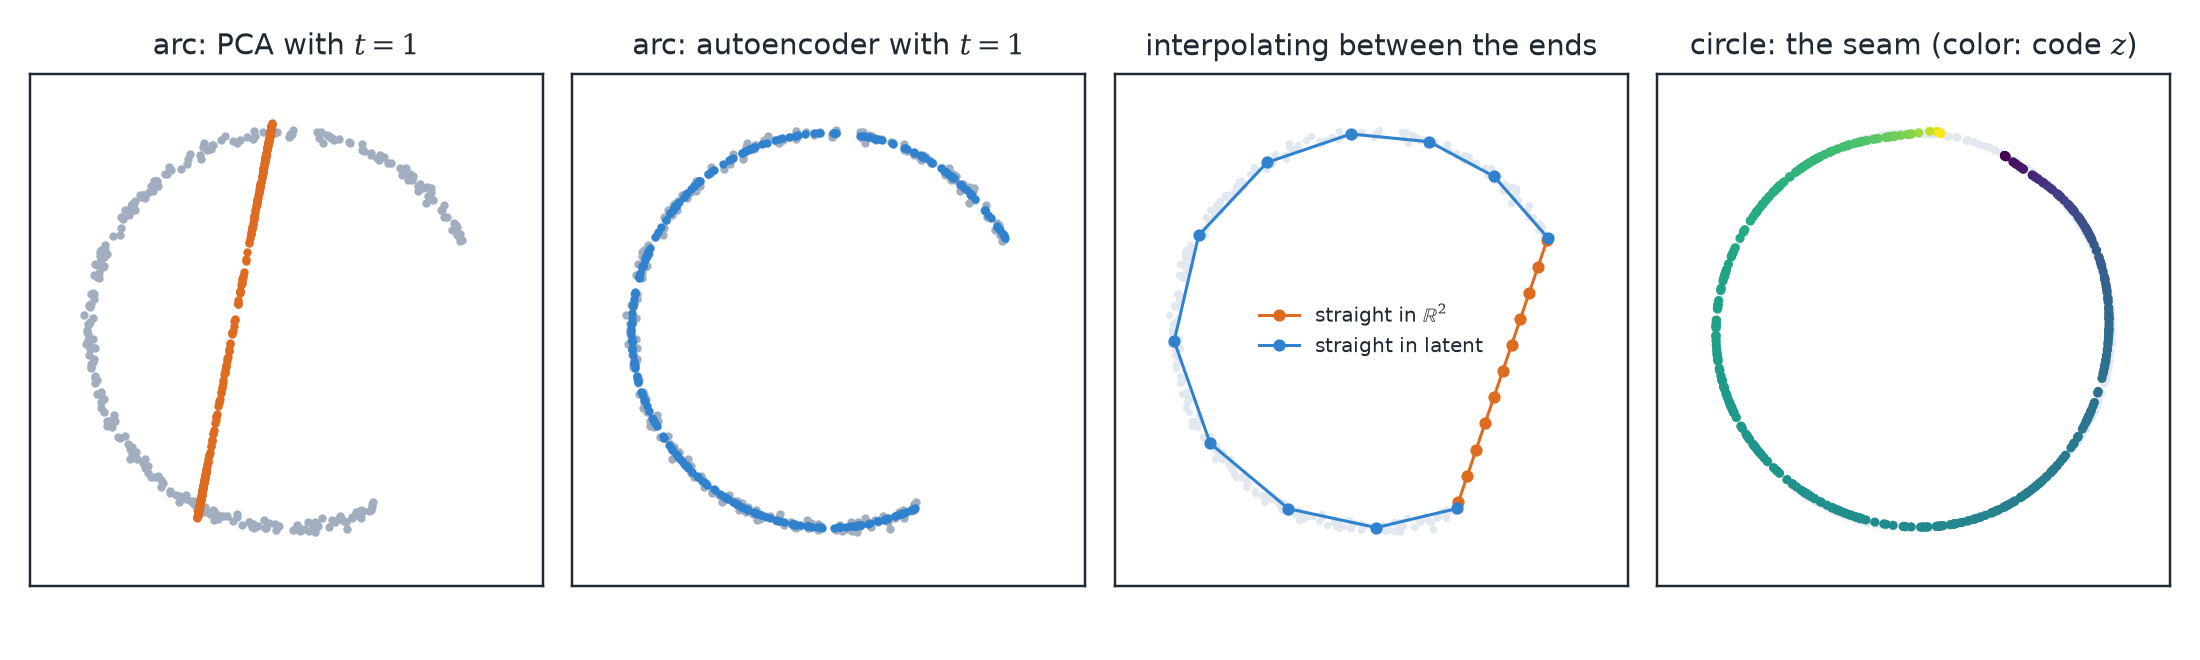
\includegraphics[width=\textwidth]{figures/ae_arc.png}
\caption{Small autoencoders actually trained on 2-D curves, $t=1$ (\texttt{tanh} layers of width $32$ or $64$ either side of the bottleneck, best of five starts). \emph{First two panels:} on an open arc, PCA must flatten everything onto a line (mean squared error $0.33$), while the autoencoder follows the curve ($0.00025$). \emph{Third:} interpolating between the ends. The straight line in $\R^2$ cuts across empty space (its midpoint has radius $0.70$), and the straight line in latent space stays on the curve (radius $0.997$ to $1.01$). \emph{Fourth:} on a closed circle, the code must run through a jump: the seam appears as the gap at the top, where the largest error ($0.33$) occurs and the code changes sharply. This is the wall from Example~\ref{ex:aecircle}.}
\label{fig:aearc}
\end{figure}

\subsection{What the way back buys you}

\begin{itemize}[nosep]
\item \textbf{New points in both directions.} Any new $\vx$ can be encoded directly, and any latent $\bm y$ can be decoded. Earlier methods embed only their training points, without extra machinery.
\item \textbf{Interpolation on the manifold.} A straight line between two data points in $\R^d$ cuts through empty space: the midpoint of two points on a Swiss roll is not on the roll. Instead, encode them, interpolate in latent space, and decode: $D\big((1-\alpha)E(\vx_1)+\alpha E(\vx_2)\big)$. If the latent space is well organized, this path stays near the manifold.
\item \textbf{Generating new data.} Decoding a latent point that came from no training example creates a new data point.
\end{itemize}

\textbf{Seeing it on real images.} Figures~\ref{fig:aedigits}--\ref{fig:aeinterp} use the same $1797$ digit images as the UMAP figures, with a bottleneck of only $t=2$ (layers $64\to128\to32\to2\to32\to128\to64$).

\begin{figure}[htbp]
\centering
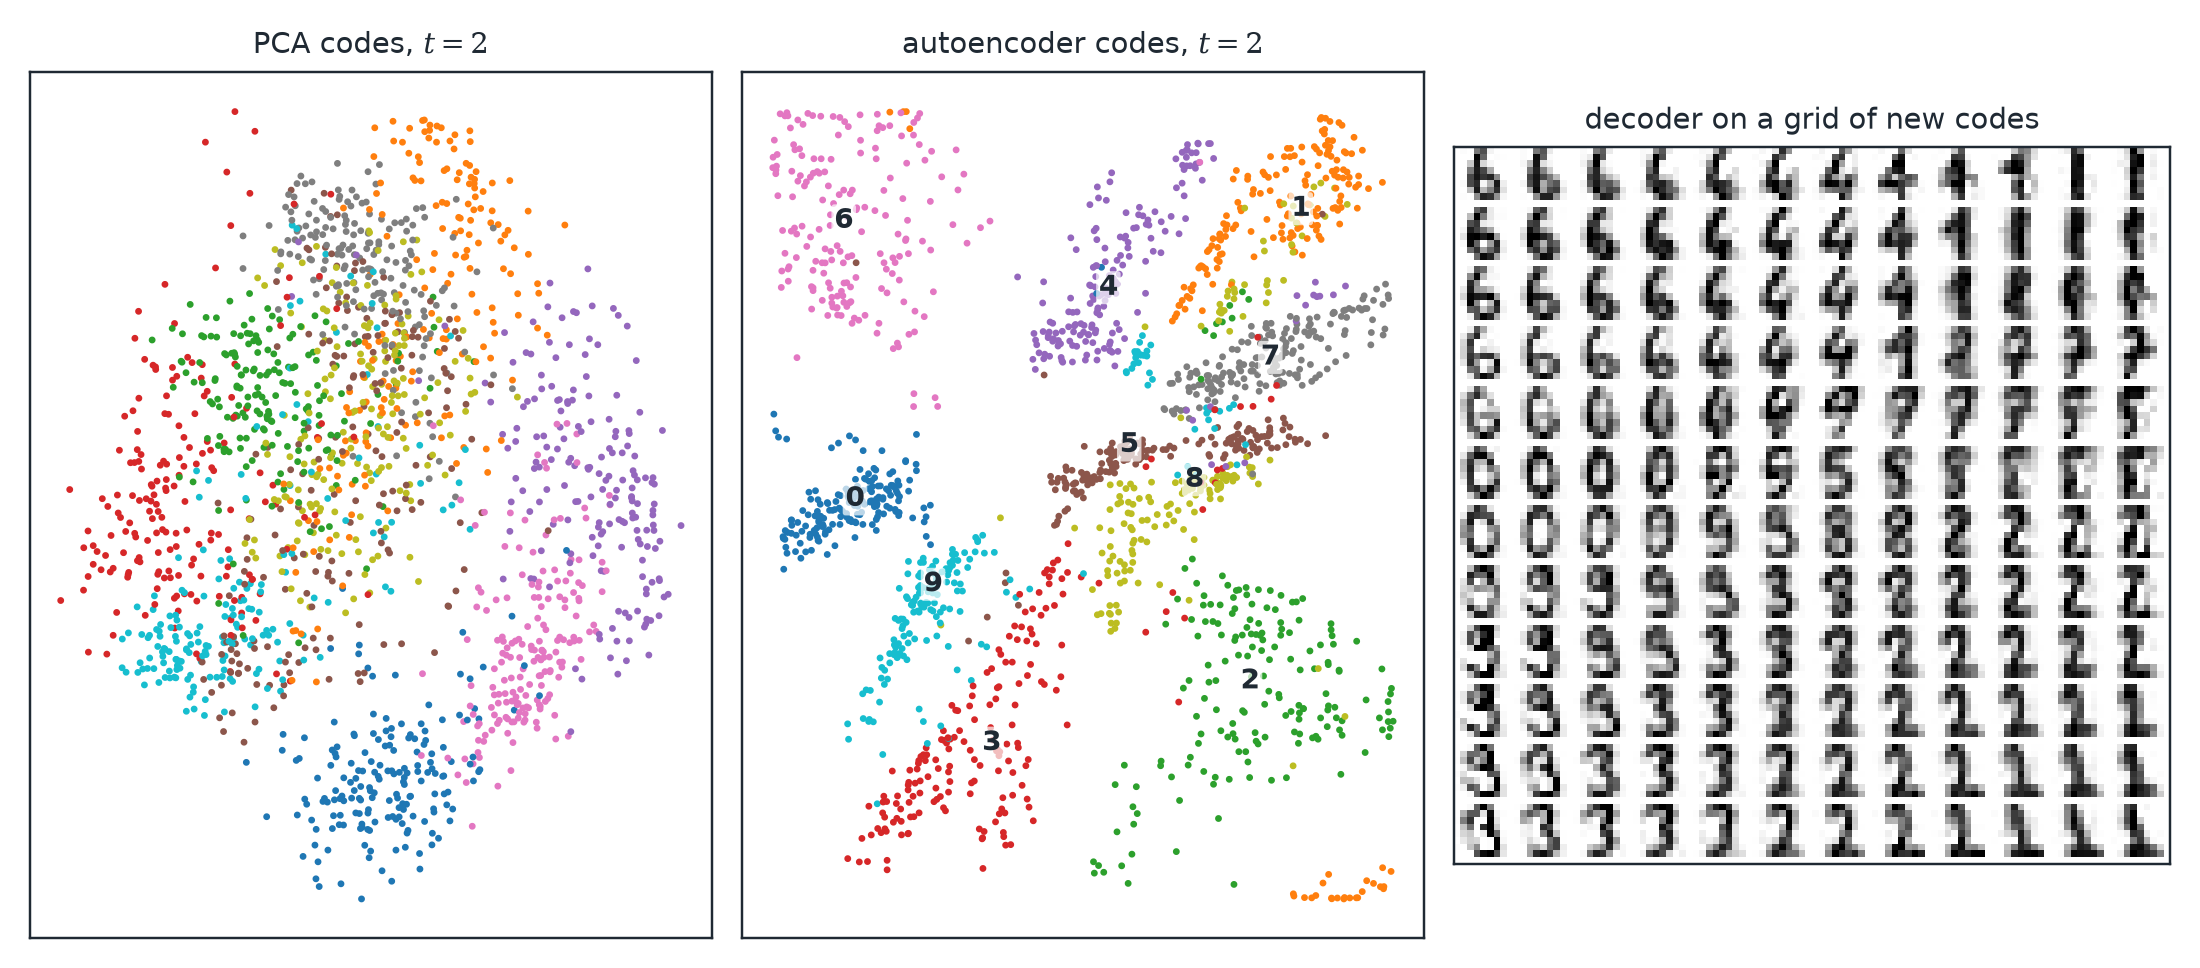
\includegraphics[width=\textwidth]{figures/ae_digits.png}
\caption{\emph{Left and middle:} the two numbers each method keeps for every image, colored by digit (labels were not used). The nonlinear codes separate the digits much better than PCA's. Reconstruction error per pixel is $0.022$ against $0.052$ for PCA, with pixels on a $0$--$1$ scale. \emph{Right:} the decoder applied to a grid of codes, most of which belong to no training image. This is generation: the digits morph smoothly from one region to the next, and tiles between regions look like blends rather than clean digits.}
\label{fig:aedigits}
\end{figure}

\begin{figure}[htbp]
\centering
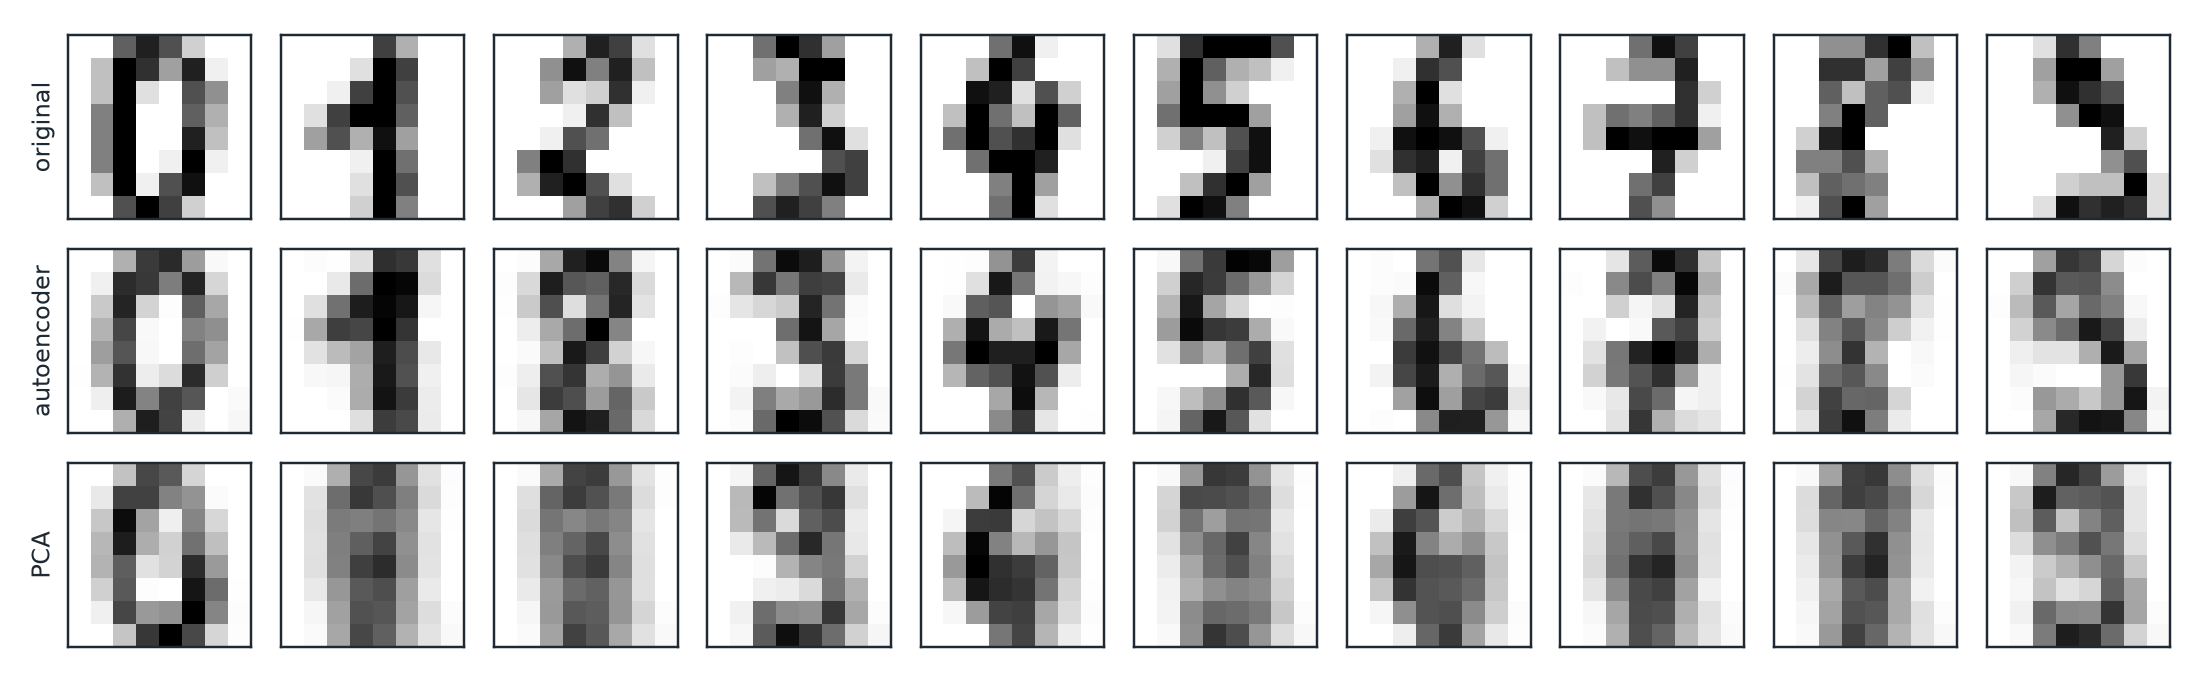
\includegraphics[width=0.9\textwidth]{figures/ae_recon.png}
\caption{The same ten images squeezed through two numbers. The autoencoder keeps most digits recognizable. PCA's rank-$2$ reconstruction can only mix two fixed patterns with the mean, so many digits turn into nearly the same blur.}
\label{fig:aerecon}
\end{figure}

\begin{figure}[htbp]
\centering
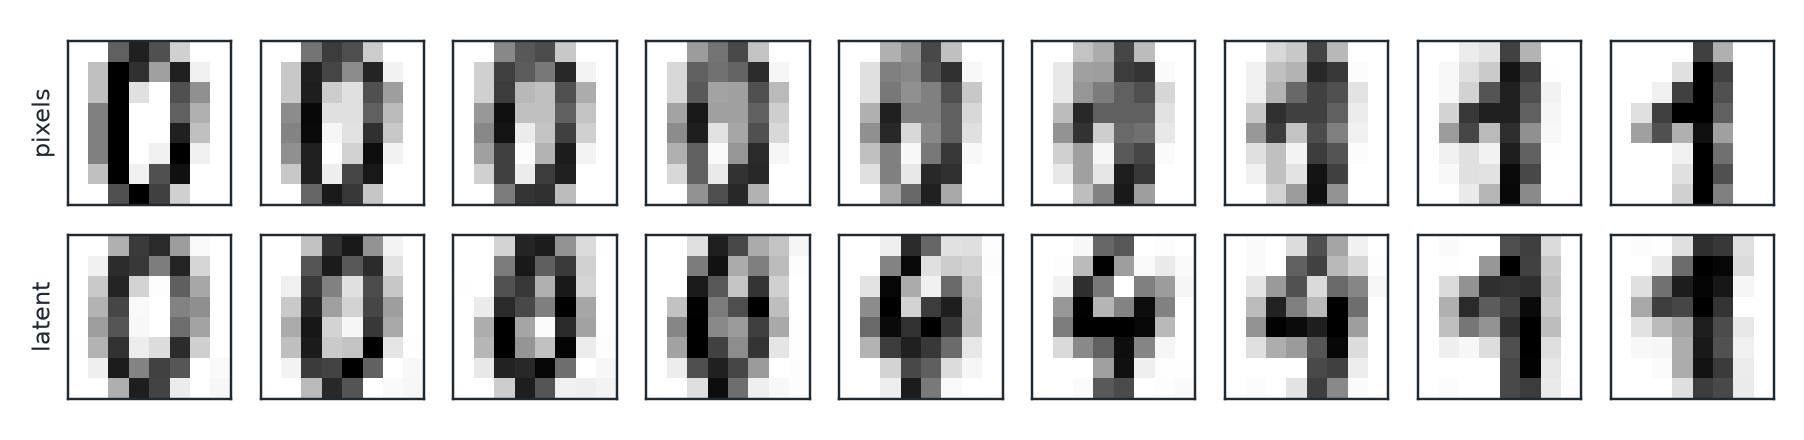
\includegraphics[width=0.82\textwidth]{figures/ae_interp.png}
\caption{Going from a $0$ to a $1$. \emph{Top:} averaging pixels gives a double exposure, with both digits ghosted on top of each other. \emph{Bottom:} a straight line in latent space gives sharper shapes, but it also passes through a $4$-like shape on the way, because the path crosses whatever lies between the two codes.}
\label{fig:aeinterp}
\end{figure}

\begin{careful}
\textbf{Nothing in the loss guarantees a well-organized latent space.} Reconstruction only constrains the decoder at the codes of the training points. A very flexible network can memorize them, even through a narrow bottleneck, by assigning arbitrary codes, and a random latent point may decode to nonsense. So $t<d$ is necessary to rule out the identity, but it does not by itself guarantee that the network has learned the manifold. Models such as variational autoencoders add structure to the latent space to address this. Also, unlike PCA, the training is nonconvex: the answer depends on the initialization, and the solutions are not nested in $t$.
\end{careful}

\subsection{Choosing the architecture}

Each layer is the same move, an affine map followed by an activation:
\[
\bm z^{(1)}=\sigma_1\big(A^{(1)}\vx+\bm b^{(1)}\big),\qquad \bm z^{(2)}=\sigma_2\big(A^{(2)}\bm z^{(1)}+\bm b^{(2)}\big),\qquad\dots
\]
The encoder is the first stack of these (high dimension down to the bottleneck), and the decoder is the second (back up to $d$). Training fits every $A^{(\ell)}$ and $\bm b^{(\ell)}$ at once by stochastic gradient descent, and backpropagation is the chain rule applied through the stack. What you choose before training:
\begin{itemize}[nosep]
\item \textbf{the number of layers} (depth);
\item \textbf{the width of each layer}, including the bottleneck width $t$;
\item \textbf{the activation functions};
\item \textbf{regularization}, such as a penalty on the weights or on the codes (sparsity, below);
\item \textbf{the data and the training length}, since more of either lets a bigger network fit.
\end{itemize}

\textbf{Symmetry is a convention.} Autoencoders are usually built as mirror images around the bottleneck, such as $64\to24\to12\to24\to64$ or $100\to64\to2\to64\to100$. The digit figures above used $64\to128\to32\to2\to32\to128\to64$. Nothing requires the decoder to mirror the encoder; it is a sensible default that gives the two halves similar capacity.

\textbf{Overfitting.} Count the parameters in $64\to24\to12\to24\to64$: the weights are $64\cdot24+24\cdot12+12\cdot24+24\cdot64=3648$ and the biases $24+12+24+64=124$, so $3772$ numbers. With that many parameters and only a few hundred training points, the network can memorize the training set, which is the warning in the box above. \textbf{Regularization} adds a penalty such as $\lambda\sum_\ell\Fro{A^{(\ell)}}^2$ to the loss, which pulls the weights toward zero and makes extreme fits expensive.

\textbf{Match the network to the geometry of the data.} This is the idea behind \textbf{geometric deep learning}: build the data's symmetries into the layers instead of making the network learn them.
\begin{itemize}[nosep]
\item \textbf{Images: convolutional networks (CNNs).} One small filter slides across the whole image, so shifting the image shifts the features the same way (\emph{translation equivariance}). The filter is shared across positions, so there are far fewer parameters than in a dense layer.
\item \textbf{Text and time series: recurrent networks (RNNs, LSTMs).} The same weights are applied at every time step, so the network accepts sequences of any length and recognizes a pattern wherever in the sequence it occurs.
\end{itemize}
For a full treatment, see Melanie Weber's AM~220.

\begin{careful}
\textbf{``Temporal invariance'' is loose.} An RNN's output is not unchanged when you shift the sequence; what is unchanged is the \emph{rule} applied at each step, because the weights are shared across time. The same goes for CNNs: shifting the input shifts the feature map (equivariance), and only a final pooling step makes the output fully unchanged (invariance).
\end{careful}

\begin{figure}[htbp]
\centering
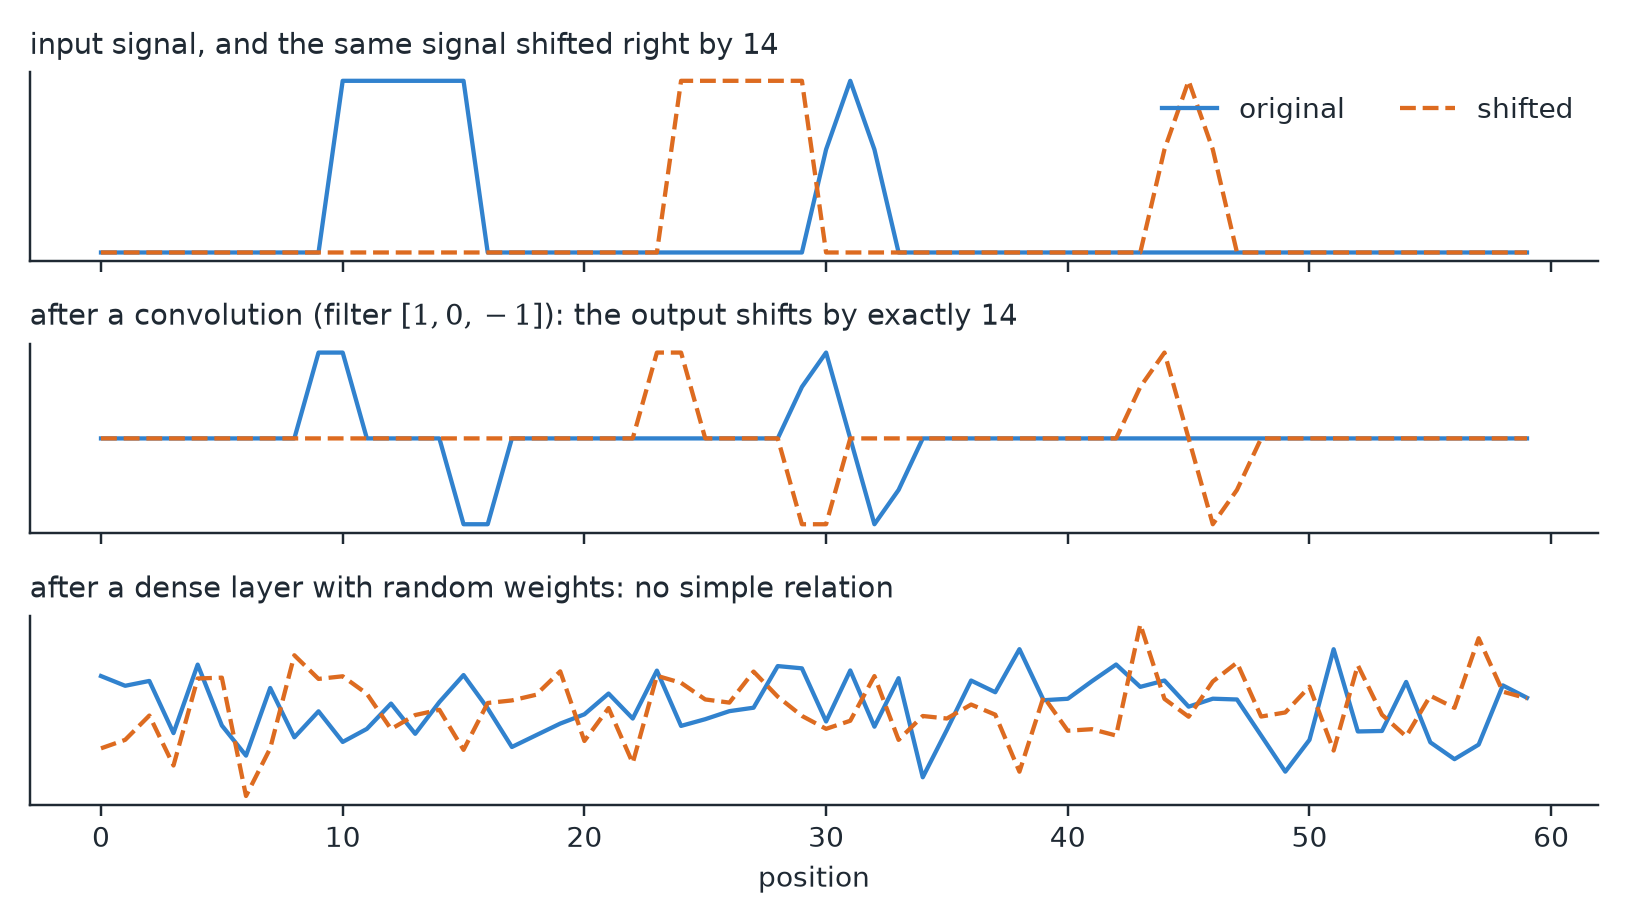
\includegraphics[width=0.8\textwidth]{figures/cnn_equiv.png}
\caption{Equivariance, in one dimension. A convolution applies the same small filter (here $(1,0,-1)$, which responds to edges) at every position, so shifting the input by $14$ shifts the output by exactly $14$ (largest difference $0$). A dense layer gives every position its own weights, so the two outputs have no simple relation (they differ by up to $2.17$ after undoing the shift).}
\label{fig:cnnequiv}
\end{figure}

\subsection{Variants}

\textbf{Denoising autoencoder.} Corrupt each input and ask for the \emph{clean} original back:
\[
\min\ \frac1N\sum_{i=1}^N\norm{\vx_i-D\big(E(\vx_i+\bm\varepsilon_i)\big)}^2,\qquad \bm\varepsilon_i\text{ fresh random noise each time}.
\]
The identity map no longer scores zero, since it would return the noise too. So the network has to learn what clean data look like, even without a narrow bottleneck. This is the standard tool for recovering damaged or noisy images.

Geometrically, a denoising autoencoder learns a map that pulls each nearby point back onto the data manifold, a learned projection (Figure~\ref{fig:aedenoise}).

\begin{figure}[htbp]
\centering
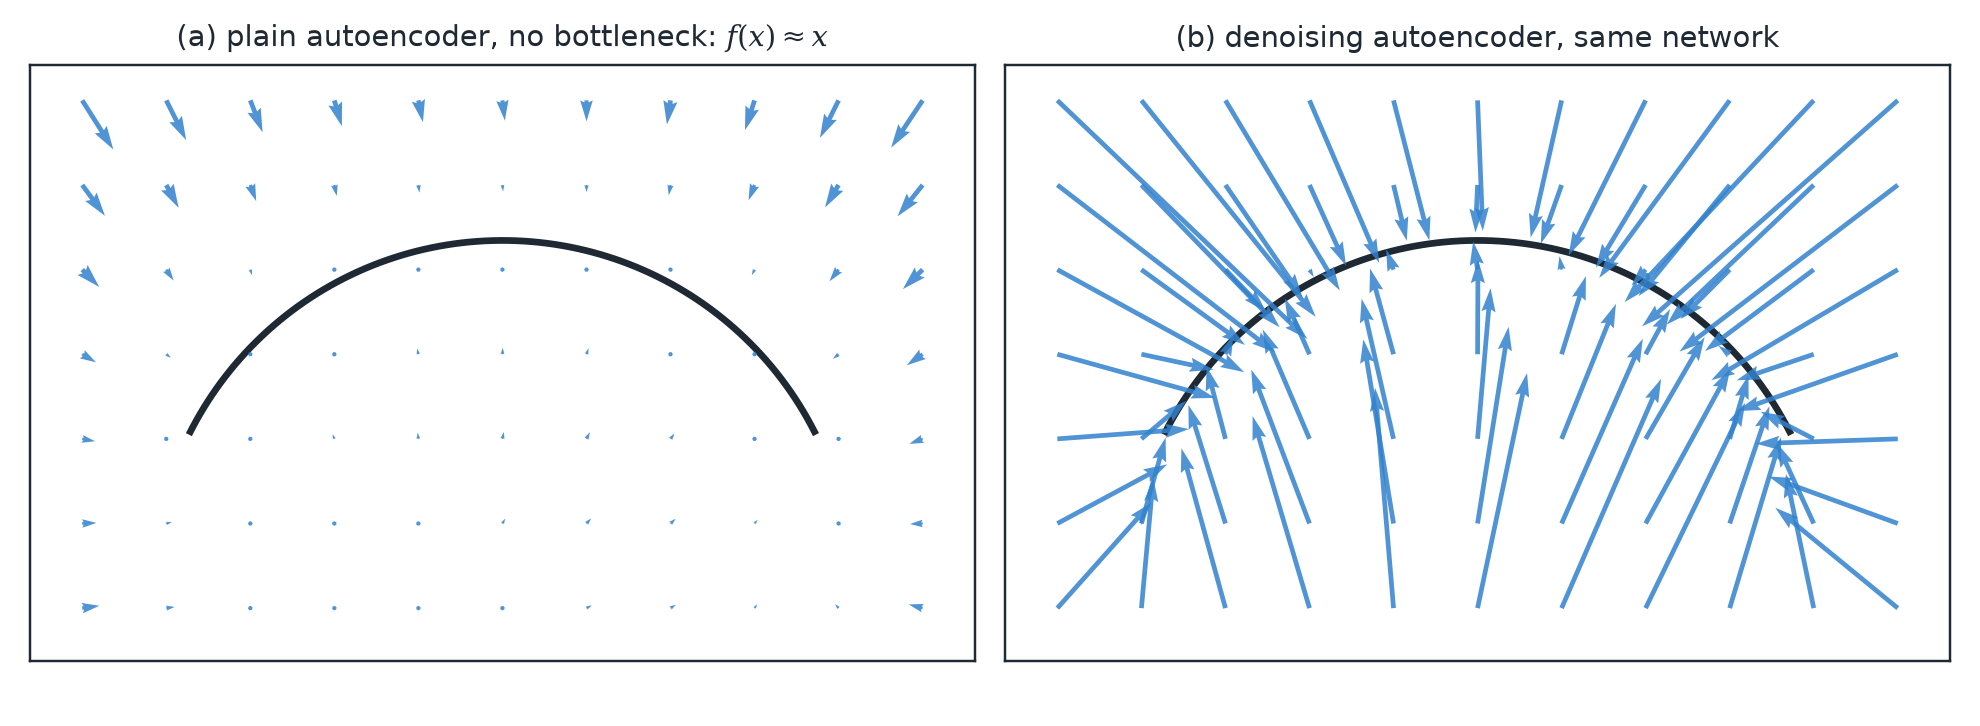
\includegraphics[width=0.95\textwidth]{figures/ae_denoise.png}
\caption{Two networks with the same architecture (two hidden layers of $64$ \texttt{tanh} units, no bottleneck), trained on $300$ points of an arc. Each arrow goes from a grid point $\vx$ to the output $f(\vx)$. \emph{(a)} Trained to reproduce clean points, the network learns nearly the identity: near the data the arrows almost vanish (median length $0.02$), and noisy points stay noisy (mean distance to the arc $0.113$ before, $0.104$ after). The larger arrows at the top corners are far from any training point, where the network is only extrapolating. \emph{(b)} Trained to map noisy copies ($\sigma=0.15$, $15$ per point) to the clean point, the network sends every arrow to the arc, from inside and from outside, and the mean distance falls from $0.113$ to $0.019$.}
\label{fig:aedenoise}
\end{figure}

\textbf{Sparse autoencoder.} Penalize the codes instead of only the weights, for example by adding $\lambda\sum_i\norm{E(\vx_i)}_1$. Then only a few code entries are nonzero for each input. The code can be even \emph{wider} than $d$, and the sparsity, not the width, keeps it from copying the input. Each code coordinate tends to switch on for one recognizable pattern, which makes the individual features interpretable.

\textbf{Variational autoencoder (VAE).} The encoder outputs a \emph{distribution} over the latent space instead of a single point, usually a normal $q(\bm y\mid\vx)=\mathcal N\big(\bm\mu(\vx),\operatorname{diag}\bm\sigma^2(\vx)\big)$, and the decoder gives a distribution over $\vx$ for each $\bm y$. Training maximizes the \textbf{evidence lower bound} (ELBO):
\[
\underbrace{\mathbb E_{\bm y\sim q(\cdot\mid\vx)}\big[\log p(\vx\mid\bm y)\big]}_{\text{reconstruct well}}\;-\;\underbrace{\mathrm{KL}\big(q(\bm y\mid\vx)\,\big\|\,\mathcal N(\bm0,I)\big)}_{\text{keep codes near a standard normal}} .
\]
This is the Bayesian version of the autoencoder: a probabilistic map from data to latent state. The second term addresses the box above. It packs the codes into one standard-normal blob without gaps, so a random draw $\bm y\sim\mathcal N(\bm0,I)$ decodes to something data-like. That makes the VAE a generative model.

\begin{figure}[htbp]
\centering
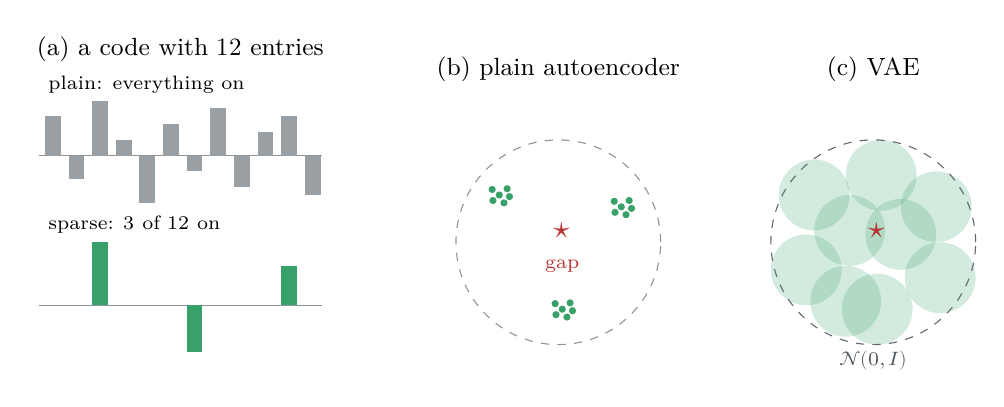
\begin{tikzpicture}[>=Stealth]
% (a) dense versus sparse codes
\begin{scope}
\node[font=\small] at (1.8,3.85) {(a) a code with $12$ entries};
\draw[ink!50] (0,2.5) -- (3.6,2.5); \draw[ink!50] (0,0.6) -- (3.6,0.6);
\foreach \h [count=\i] in {0.5,-0.3,0.7,0.2,-0.6,0.4,-0.2,0.6,-0.4,0.3,0.5,-0.5}
  \fill[ink!45] ({0.3*\i-0.22},2.5) rectangle ({0.3*\i-0.02},{2.5+\h});
\foreach \h [count=\i] in {0,0,0.8,0,0,0,-0.6,0,0,0,0.5,0}
  \fill[accentD] ({0.3*\i-0.22},0.6) rectangle ({0.3*\i-0.02},{0.6+\h});
\node[font=\scriptsize,anchor=west] at (0,3.4) {plain: everything on};
\node[font=\scriptsize,anchor=west] at (0,1.62) {sparse: $3$ of $12$ on};
\end{scope}
% (b) plain autoencoder latent space
\begin{scope}[shift={(6.6,1.4)}]
\node[font=\small] at (0,2.2) {(b) plain autoencoder};
\draw[dashed,ink!50] (0,0) circle (1.3);
\foreach \c in {(-0.75,0.6),(0.8,0.45),(0.05,-0.85)}
  \foreach \d in {(0,0),(0.1,0.08),(-0.09,0.07),(0.06,-0.1),(-0.08,-0.07),(0.13,-0.02)}
    \fill[accentD,shift={\c}] \d circle (1.3pt);
\node[thmred,font=\large] at (0.05,0.15) {$\star$};
\node[thmred,font=\scriptsize,align=center] at (0.05,-0.3) {gap};
\end{scope}
% (c) VAE latent space
\begin{scope}[shift={(10.6,1.4)}]
\node[font=\small] at (0,2.2) {(c) VAE};
\foreach \c in {(-0.75,0.6),(0.8,0.45),(0.05,-0.85),(-0.3,0.15),(0.35,0.1),(-0.85,-0.35),(0.85,-0.45),(0.1,0.85),(-0.35,-0.75)}
  \fill[accentD,opacity=0.22] \c circle (0.45);
\draw[dashed,ink!70] (0,0) circle (1.3);
\node[font=\scriptsize,ink!80] at (0,-1.5) {$\mathcal N(\bm0,I)$};
\node[thmred,font=\large] at (0.05,0.15) {$\star$};
\end{scope}
\end{tikzpicture}
\caption{What the extra terms do to the latent space (schematic). \emph{(a)} A sparse penalty leaves only a few code entries switched on for each input. \emph{(b)} A plain autoencoder can put its codes in tight, separated clumps. A random latent point ($\star$) lands in a gap that no training point used, and the decoder was never trained there. \emph{(c)} A VAE encodes each point as a small cloud $q(\bm y\mid\vx)$, and the KL term pulls the clouds toward the dashed standard normal. The clouds overlap and cover it, so a random draw from $\mathcal N(\bm0,I)$ lands where the decoder was trained.}
\label{fig:aelatent}
\end{figure}

\subsection{Transfer learning}

Labeled data are expensive, but unlabeled data are cheap and plentiful (for example, images posted online). An autoencoder needs no labels, so it can learn features from the large unlabeled set, and a small labeled set only has to train what sits on top.

\begin{center}
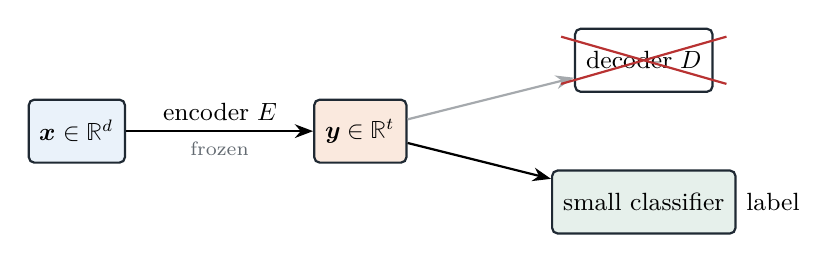
\begin{tikzpicture}[>=Stealth, bx/.style={draw=ink,thick,rounded corners=2pt,minimum height=8mm,inner sep=4pt,font=\small}]
\node[bx,fill=dataC!10] (x) at (0,0) {$\vx\in\R^d$};
\node[bx,fill=accentC!15] (y) at (3.6,0) {$\bm y\in\R^t$};
\node[bx] (d) at (7.2,0.9) {decoder $D$};
\node[bx,fill=intgreen!12] (c) at (7.2,-0.9) {small classifier};
\draw[->,thick] (x) -- node[above,font=\small]{encoder $E$} node[below,font=\scriptsize,ink!70]{frozen} (y);
\draw[->,thick,ink!40] (y) -- (d);
\draw[thick,thmred] (6.15,0.6) -- (8.25,1.2) (6.15,1.2) -- (8.25,0.6);
\draw[->,thick] (y) -- (c);
\node[font=\small,right] at (c.east) {label};
\end{tikzpicture}
\end{center}
\begin{enumerate}[nosep]
\item Train an autoencoder on the large unlabeled dataset.
\item Throw away the decoder.
\item Attach a small classifier to the bottleneck.
\item Train only the classifier, on the small labeled dataset. The encoder is frozen, or at most adjusted slightly.
\end{enumerate}
The result combines rich nonlinear features learned from unlabeled data with a classifier that has few parameters. For example, logistic regression from $t=32$ codes to $10$ classes has $33\cdot10=330$ parameters, a number a few hundred labels can support. Pretrained encoders are available for many kinds of data, so step 1 is often already done.

\begin{careful}
\textbf{What gets discarded and what gets frozen.} The \emph{decoder} is discarded, because it is only needed for training. The \emph{encoder} is kept and frozen (its weights stay fixed). Freezing the decoder would be pointless, since nothing uses it any more.
\end{careful}

\clearpage
% ==================================================================
\section{Clustering: $k$-Means, Gaussian Mixtures and Spectral Clustering}\label{sec:kmeans}
% ==================================================================

\subsection{The problem}

\textbf{Clustering} groups the data into clusters of similar points, with no labels to guide it. Before choosing an algorithm, ask \emph{what kind of relationship exists in the data}. Figure~\ref{fig:kmshapes} shows three kinds of cluster: round blobs, clusters stretched along a direction, and nested rings. One algorithm will not handle all three.

\begin{definition}{Partition and centers}{partition}
Given $N$ observations $\vx_1,\dots,\vx_N\in\R^d$ and a number $k$, a \textbf{partition} into $k$ clusters is a collection of sets $\mathcal C_1,\dots,\mathcal C_k$ with
\[
\mathcal C_l\cap\mathcal C_m=\varnothing\ \ (l\ne m),\qquad \bigcup_{l=1}^k\mathcal C_l=\{\vx_1,\dots,\vx_N\}.
\]
Each point is in exactly one cluster. \textbf{Center-based clustering} also outputs a center for each cluster, $\bm c_1,\dots,\bm c_k\in\R^d$.
\end{definition}

The $k$-means loss measures how spread out each cluster is, the \textbf{within-cluster variation}:
\[
V(\mathcal C_l)=\frac1{2|\mathcal C_l|}\sum_{\vx_i,\vx_j\in\mathcal C_l}\norm{\vx_i-\vx_j}^2
=\sum_{\vx_i\in\mathcal C_l}\norm{\vx_i-\bm c_l}^2,
\qquad \bm c_l=\frac1{|\mathcal C_l|}\sum_{\vx_i\in\mathcal C_l}\vx_i ,
\]
where $|\mathcal C_l|$ is the number of points in the cluster. The objective adds this up over the clusters:
\[
L(\mathcal C)=\sum_{l=1}^kV(\mathcal C_l)=\sum_{l=1}^k\ \sum_{\vx_i\in\mathcal C_l}\norm{\vx_i-\bm c_l}^2 .
\]

\begin{proposition}{Pairwise distances and distances to the mean}{pairwise}
For any finite set $\mathcal C$ with mean $\bm c$,
\[
\begin{aligned}
&\text{(a)}\ \ \frac1{2|\mathcal C|}\sum_{\vx_i,\vx_j\in\mathcal C}\norm{\vx_i-\vx_j}^2=\sum_{\vx_i\in\mathcal C}\norm{\vx_i-\bm c}^2,\\
&\text{(b)}\ \ \sum_{\vx_i\in\mathcal C}\norm{\vx_i-\bm m}^2=\sum_{\vx_i\in\mathcal C}\norm{\vx_i-\bm c}^2+|\mathcal C|\,\norm{\bm c-\bm m}^2\ \text{ for any }\bm m .
\end{aligned}
\]
So by (b), the mean is the single best center for a cluster.
\end{proposition}
\begin{proofsketch}
Write $\bm u_i=\vx_i-\bm c$, so $\sum_i\bm u_i=\bm0$. For (a), $\norm{\vx_i-\vx_j}^2=\norm{\bm u_i}^2+\norm{\bm u_j}^2-2\bm u_i\T\bm u_j$. Summing over all $i,j$ gives $2|\mathcal C|\sum_i\norm{\bm u_i}^2-2\norm{\sum_i\bm u_i}^2=2|\mathcal C|\sum_i\norm{\bm u_i}^2$. For (b), expand $\norm{\bm u_i+(\bm c-\bm m)}^2$; the cross term is $2(\bm c-\bm m)\T\sum_i\bm u_i=0$.
\end{proofsketch}

\begin{intuition}
\textbf{The key step: move the origin to the centroid.} Think of $\bm u_i=\vx_i-\bm c$ as the arrow that starts at the centroid and ends at $\vx_i$. It says how far, and in which direction, point $i$ is from the center. For example, if $\bm c=(3,4)$ and $\vx_i=(5,7)$, then $\bm u_i=(2,3)$.

These arrows always balance out. Writing $n=|\mathcal C|$,
\[
\sum_i\bm u_i=\sum_i(\vx_i-\bm c)=\sum_i\vx_i-n\bm c=\sum_i\vx_i-\sum_i\vx_i=\bm0,
\]
because the definition of the mean, $\bm c=\frac1n\sum_i\vx_i$, says exactly that $n\bm c=\sum_i\vx_i$. In one dimension: the points $1,2,6$ have mean $3$, and the deviations $-2,-1,3$ add to $0$.

The proof uses this twice, and both times it kills a term.
\begin{itemize}
\item \textbf{In (a):} the cross terms add up to $\sum_{i,j}\bm u_i\T\bm u_j=\big(\sum_i\bm u_i\big)\T\big(\sum_j\bm u_j\big)=\norm{\textstyle\sum_i\bm u_i}^2=0$.
\item \textbf{In (b):} the cross term $2(\bm c-\bm m)\T\sum_i\bm u_i$ is $0$ for every $\bm m$.
\end{itemize}
Only the centroid has this property. Measured from any other point $\bm m$, the arrows $\vx_i-\bm m$ add to $n(\bm c-\bm m)\neq\bm0$, and that leftover is the extra $n\norm{\bm c-\bm m}^2$ in (b).
\end{intuition}

\begin{example}{Part (b) in full: why the mean is the best center}{meanbest}
Let $\bm m$ be any proposed center. Get from $\bm m$ to $\vx_i$ by going through the mean:
\[
\vx_i-\bm m=\underbrace{(\vx_i-\bm c)}_{\bm u_i}+\underbrace{(\bm c-\bm m)}_{\text{same for every }i}.
\]
Square, expand, and add over $i$. The last piece does not depend on $i$, so it is counted $n$ times:
\[
\sum_i\norm{\vx_i-\bm m}^2
=\sum_i\Big[\norm{\bm u_i}^2+2\bm u_i\T(\bm c-\bm m)+\norm{\bm c-\bm m}^2\Big]
=\sum_i\norm{\bm u_i}^2+2\Big(\sum_i\bm u_i\Big)^{\!\T}(\bm c-\bm m)+n\norm{\bm c-\bm m}^2 .
\]
The middle term is $0$ because $\sum_i\bm u_i=\bm0$, which leaves
\[
\boxed{\ \sum_i\norm{\vx_i-\bm m}^2=\underbrace{\sum_i\norm{\vx_i-\bm c}^2}_{\text{loss at the mean}}+\underbrace{n\norm{\bm c-\bm m}^2}_{\text{extra loss from moving away}}\ }
\]
The extra term is never negative and is $0$ only at $\bm m=\bm c$, so the mean is the unique best center.

\textbf{Numbers.} The points $1,2,6$ have mean $c=3$ and loss $4+1+9=14$ around it. With $m=4$ instead, the loss is $9+4+4=17$, and the formula predicts $14+3\,(3-4)^2=17$.

This is why the update step of Lloyd's algorithm moves each center to the mean of the points currently assigned to it.
\end{example}

\begin{careful}
\textbf{Squaring lets far-away points pull hard.} A point at distance $r$ adds $r^2$ to the loss, so one distant point can outweigh many close ones, and the mean chases it. Add the point $30$ to $1,2,6$: the mean jumps from $3$ to $9.75$, a center that is close to none of the four points. Together with the earlier box, k-means is pulled both by \emph{large} clusters (more terms) and by \emph{far-away} points (bigger terms). An outlier can drag a center off its cluster or grab a center for itself. Robust variants replace the mean: k-medians uses absolute distances, whose best center is the coordinate-wise median ($1,2,6,30$ give $4$), and k-medoids requires each center to be one of the data points.
\end{careful}

\begin{careful}
\textbf{It is not quite the \emph{average} pairwise distance.} The double sum runs over ordered pairs, so each pair appears twice, hence the $2$. The average over all $|\mathcal C|^2$ ordered pairs would divide by $|\mathcal C|^2$, so
\[
V(\mathcal C)=\frac{|\mathcal C|}2\times\big(\text{average squared distance between two points of }\mathcal C\big).
\]
A cluster counts in proportion to its size: a big loose cluster costs more than a small loose one.
\end{careful}

\begin{intuition}
\textbf{Why ``spread around the center'' and ``spread between pairs'' agree.} Pick two points of a cluster at random. Each one sits away from the center by some arrow $\bm u_i$, so their difference is $\bm u_i-\bm u_j$. On average the two arrows point in unrelated directions, so the cross term $-2\bm u_i\T\bm u_j$ averages out (it is exactly the term that $\sum_i\bm u_i=\bm0$ kills), and the squared distance is on average the sum of the two squared lengths. That is why a typical pair is about $\sqrt2$ times as far apart as a typical point is from the center, and why the two ways of measuring spread differ only by a constant factor. \textbf{Check:} for $1,2,6$, the ordered pairs give $2(1^2+5^2+4^2)=84$, and $84/(2\cdot3)=14$, which is the loss around the mean $3$.
\end{intuition}

\begin{intuition}
\textbf{$k$-means is compression too.} Replace every point by its cluster's center. Then $L$ is exactly the reconstruction error, $\sum_i\norm{\vx_i-\widehat{\vx}_i}^2$, with the reconstructions restricted to a ``codebook'' of $k$ points. PCA restricts them to a $t$-dimensional plane and an autoencoder to a learned curved surface; $k$-means restricts them to $k$ points.
\end{intuition}

\begin{figure}[htbp]
\centering
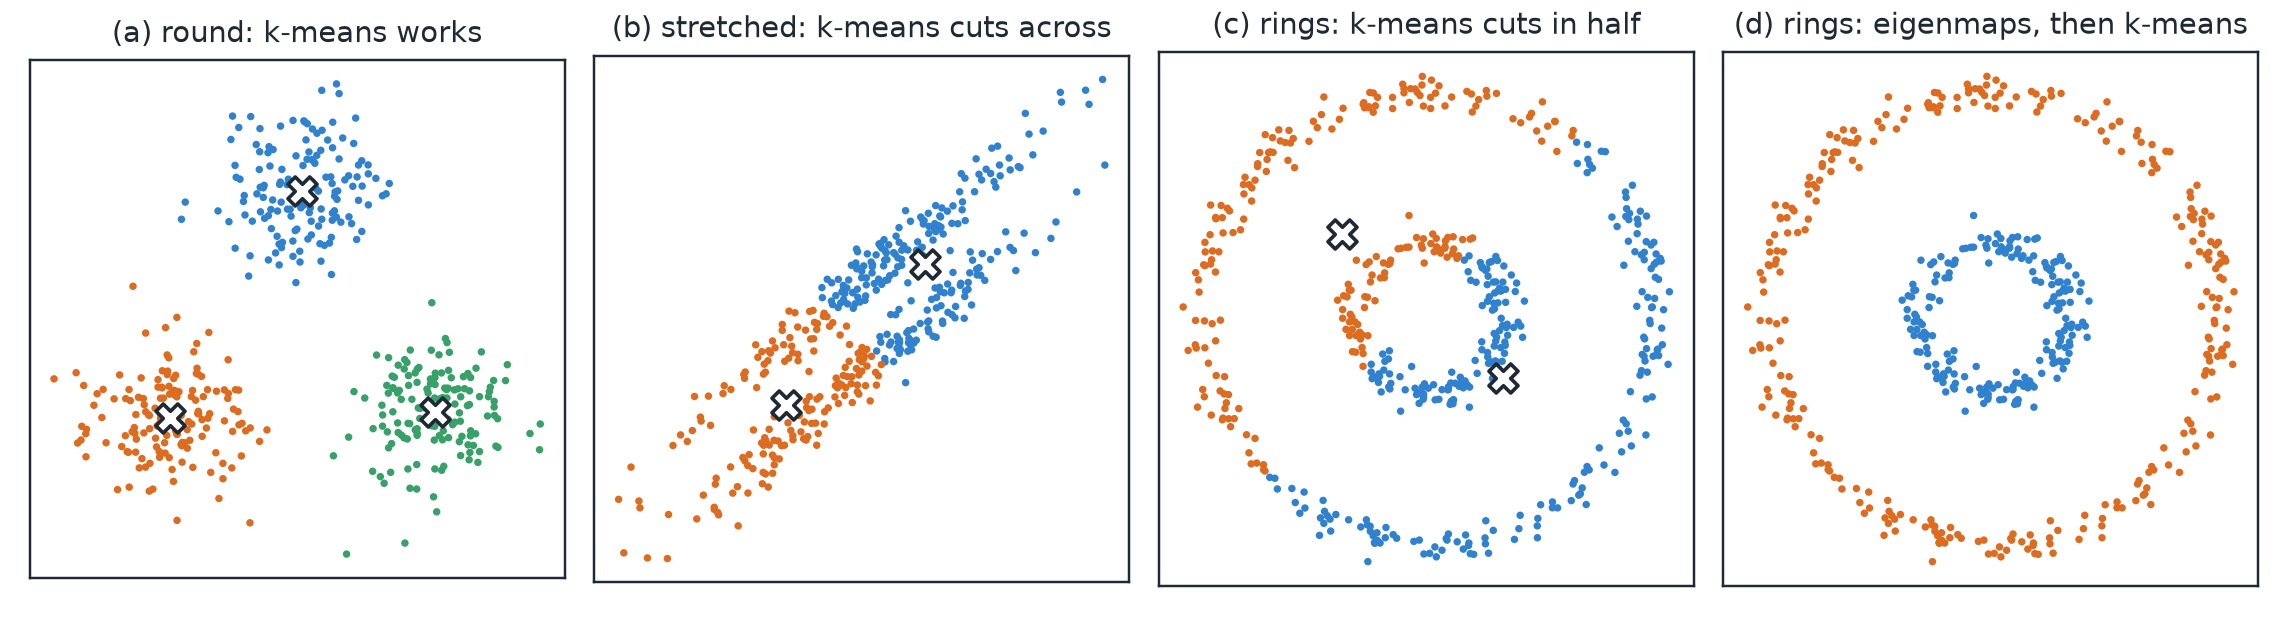
\includegraphics[width=\textwidth]{figures/kmeans_shapes.png}
\caption{$k$-means (best of $10$ starts; crosses mark centers) on three cluster shapes. \emph{(a)} Round, well-separated blobs: correct. \emph{(b)} Two long, parallel clusters: $k$-means splits them crosswise instead, matching the true groups for only $62.5\%$ of points. \emph{(c)} Two rings: it cuts both in half ($54\%$, barely better than a coin flip). \emph{(d)} The same rings clustered from a $10$-nearest-neighbor graph (Laplacian eigenmaps, then $k$-means on the embedding, which is spectral clustering): $100\%$ correct.}
\label{fig:kmshapes}
\end{figure}

\textbf{Why $k$-means wants round clusters.} Each point goes to its nearest center, so cluster $l$ is the set of points closer to $\bm c_l$ than to any other center. The boundary between two clusters is the perpendicular bisector of their centers, a straight line (a hyperplane in $\R^d$), and every cluster is a convex region. A ring cannot be carved out with straight cuts, and two long parallel clusters are cheaper to cut across than along (Figure~\ref{fig:kmshapes}). To see why the boundary is straight, compare the two squared distances:
\[
\norm{\vx-\bm c_1}^2<\norm{\vx-\bm c_2}^2
\iff -2\bm c_1\T\vx+\norm{\bm c_1}^2<-2\bm c_2\T\vx+\norm{\bm c_2}^2
\iff 2(\bm c_2-\bm c_1)\T\vx<\norm{\bm c_2}^2-\norm{\bm c_1}^2 .
\]
The $\norm{\vx}^2$ is the same on both sides and cancels, and what is left is linear in $\vx$, so it describes a half-space. The tie line goes through the midpoint of the two centers and is perpendicular to $\bm c_2-\bm c_1$. A Gaussian mixture keeps a different $\vx\T\Sigma_j^{-1}\vx$ term for each component, which does not cancel, so its boundaries can curve.

\textbf{Seeing it.} Figure~\ref{fig:kmbisector}(a) shows the rule for one point: $\vx$ is $2.02$ from $\bm c_1$ and $1.84$ from $\bm c_2$, so it lands on $\bm c_2$'s side of the bisector. With more centers, panel (b), the bisectors carve the plane into convex polygons (a \textbf{Voronoi diagram}). A ring around the middle passes through five different cells, so no single cell can hold it.

\textbf{Why long clusters get cut across.} In panels (c) and (d), $400$ points lie in two parallel strips, $8$ long and $1.2$ apart. The true split leaves each point spread along a strip of length $8$, and a uniform spread over length $8$ has variance $8^2/12\approx5.3$ per point, so $L=2001$. Cutting both strips in half at $x=0$ shortens each piece to length $4$ (variance $4^2/12\approx1.3$) and only adds the vertical offset $0.6^2=0.36$, so $L=689$, $2.9$ times smaller. $k$-means is doing its job: it minimizes $L$, and $L$ simply prefers compact pieces to the true strips.

\begin{figure}[htbp]
\centering
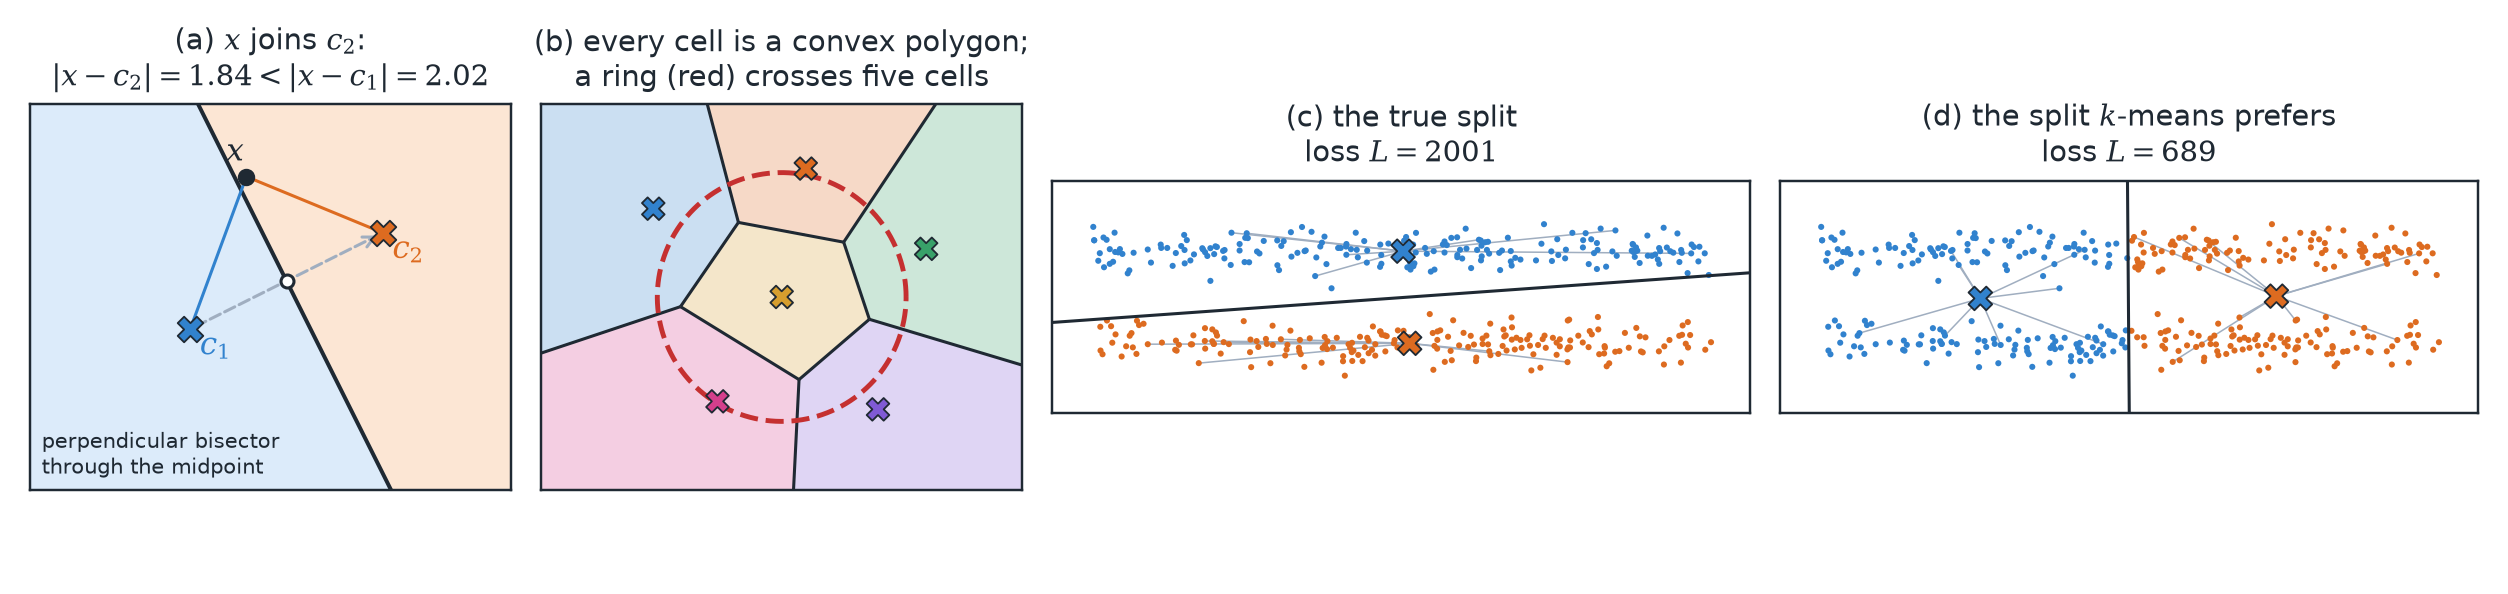
\includegraphics[width=\textwidth]{figures/kmeans_bisector.png}
\caption{The geometry of the nearest-center rule. \emph{(a)} The boundary between two centers is the perpendicular bisector through their midpoint (open circle). \emph{(b)} Six centers give six convex cells; the red ring crosses five of them. \emph{(c)} Two long strips, split correctly: $L=2001$. Gray lines join a few points to their centers, and many of them are long. \emph{(d)} The crosswise split: $L=689$. Every point is near its center, so $k$-means prefers this wrong answer.}
\label{fig:kmbisector}
\end{figure}

\textbf{How a GMM's boundary bends.} Figure~\ref{fig:kmgmmbound} uses a tight component at $(0,0)$ with standard deviation $0.35$ and a broad one at $(2.6,0)$ with standard deviations $1.6$ and $1.1$. $k$-means splits the plane at the bisector $x=1.3$. The GMM's boundary, where the two weighted densities are equal, is a closed curve around the tight component: along the axis, blue wins only from $x=-1.15$ to $x=0.89$. Two things change. The tight component claims less on the side facing the broad one, since $x=1$ is about $3$ of its standard deviations from its center but only $1$ of the broad one's. And a point far to the \emph{left}, such as $x=-2$, goes to the broad component even though it is on the tight one's side: the broad Gaussian's tails decay more slowly.

\begin{figure}[htbp]
\centering
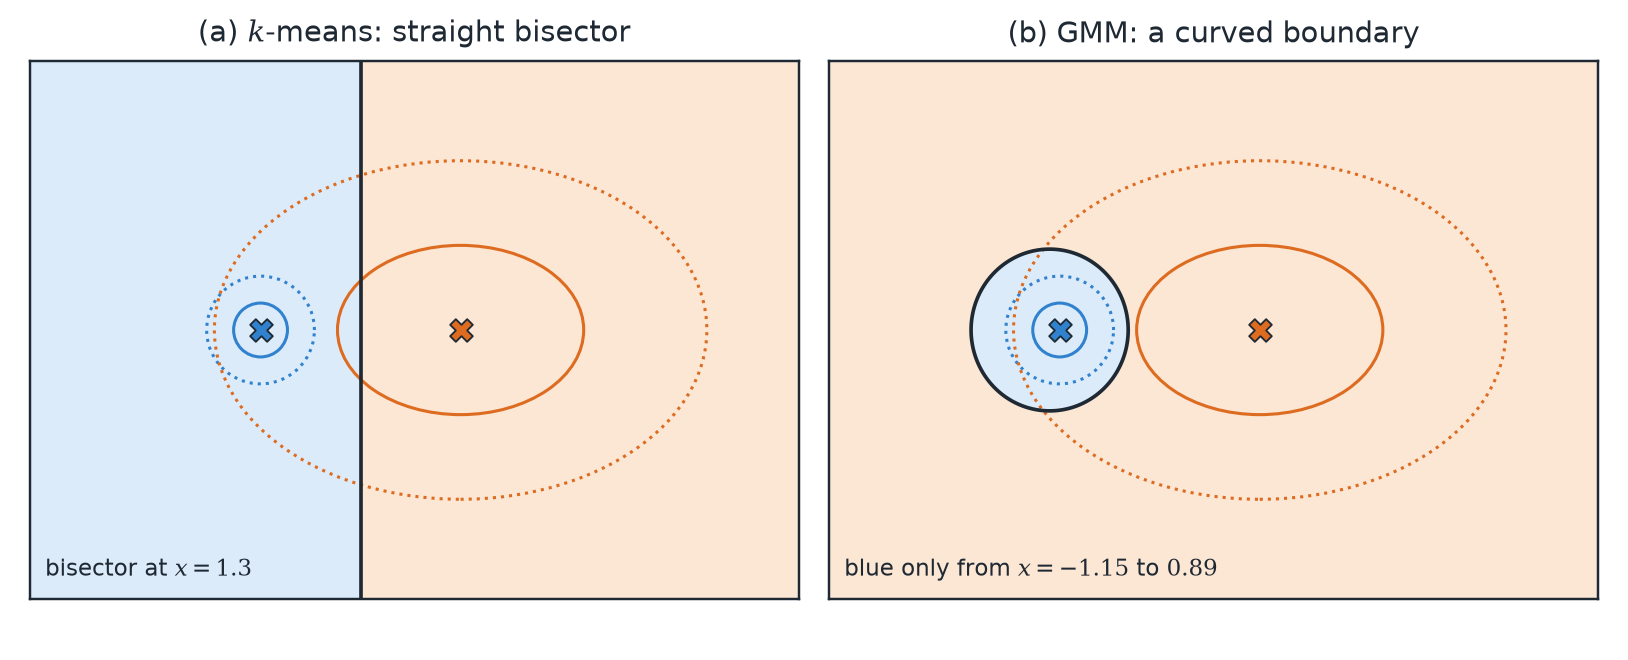
\includegraphics[width=0.78\textwidth]{figures/kmeans_vs_gmm_boundary.png}
\caption{The same two clusters, assigned by $k$-means and by a GMM. Ellipses are $1$ (solid) and $2$ (dotted) standard deviations. \emph{(a)} $k$-means ignores the spreads and cuts at the bisector $x=1.3$. \emph{(b)} The GMM boundary is a closed curve: the tight component's region is a small disk around it, running from $x=-1.15$ to $0.89$ along the axis, and the broad component claims everything else.}
\label{fig:kmgmmbound}
\end{figure}

\textbf{Why the GMM boundary curves: the algebra.} A point goes to component $1$ when $\log\big(p_1\mathcal N(\vx;\bm\mu_1,\Sigma_1)\big)>\log\big(p_2\mathcal N(\vx;\bm\mu_2,\Sigma_2)\big)$. Taking the log of the Gaussian density,
\[
\log\big(p_j\,\mathcal N(\vx;\bm\mu_j,\Sigma_j)\big)=\log p_j-\tfrac12\log|\Sigma_j|-\tfrac d2\log2\pi-\tfrac12(\vx-\bm\mu_j)\T\Sigma_j^{-1}(\vx-\bm\mu_j),
\]
and expanding the quadratic form (using $\vx\T\Sigma_j^{-1}\bm\mu_j=\bm\mu_j\T\Sigma_j^{-1}\vx$, since $\Sigma_j^{-1}$ is symmetric),
\[
(\vx-\bm\mu_j)\T\Sigma_j^{-1}(\vx-\bm\mu_j)=\vx\T\Sigma_j^{-1}\vx-2\bm\mu_j\T\Sigma_j^{-1}\vx+\bm\mu_j\T\Sigma_j^{-1}\bm\mu_j .
\]
Subtract the two. The $\frac d2\log2\pi$ cancels, but the $\vx\T\Sigma_j^{-1}\vx$ terms cancel only if $\Sigma_1=\Sigma_2$:
\[
\begin{aligned}
g(\vx)&=-\tfrac12\,\vx\T\big(\Sigma_1^{-1}-\Sigma_2^{-1}\big)\vx+\big(\Sigma_1^{-1}\bm\mu_1-\Sigma_2^{-1}\bm\mu_2\big)\T\vx+\kappa,\\
\kappa&=\log\tfrac{p_1}{p_2}-\tfrac12\log\tfrac{|\Sigma_1|}{|\Sigma_2|}-\tfrac12\big(\bm\mu_1\T\Sigma_1^{-1}\bm\mu_1-\bm\mu_2\T\Sigma_2^{-1}\bm\mu_2\big)\quad(\text{a constant}).
\end{aligned}
\]
The boundary is $g(\vx)=0$. In two dimensions that is $ax_1^2+bx_1x_2+cx_2^2+dx_1+ex_2+f=0$, a \textbf{conic section}, and the sign of $b^2-4ac$ says which kind (Figure~\ref{fig:gmmconics}):
\begin{itemize}[nosep]
\item \textbf{Shared covariance, $\Sigma_1=\Sigma_2$:} $a=b=c=0$, and the boundary is a straight line, as in $k$-means but tilted by $\Sigma$. This is why the shared-covariance models (EEE and its relatives) give straight boundaries. $k$-means is the special case $\Sigma_j=\sigma^2I$, $p_1=p_2$, where the line is the perpendicular bisector.
\item \textbf{$b^2-4ac<0$: an ellipse.} This happens when one component is tighter than the other in \emph{every} direction. In Figure~\ref{fig:kmgmmbound}, the tight component's precision is $1/0.35^2=8.2$ in both directions, against $1/1.6^2=0.39$ and $1/1.1^2=0.83$ for the broad one. The coefficients are $a=-3.89$, $c=-3.67$, $d=-1.02$, $b=e=0$, $f=3.99$. On the axis $x_2=0$ the boundary solves $-3.89x_1^2-1.02x_1+3.99=0$, whose roots are exactly the endpoints $x_1=-1.15$ and $0.89$ seen there.
\item \textbf{$b^2-4ac>0$: a hyperbola.} This happens when each component is tighter in a \emph{different} direction. In panel (c), the wide component wins far to the left and far to the right, so its region is two separate pieces.
\end{itemize}
In $d$ dimensions the same rule applies to the eigenvalues of $\Sigma_1^{-1}-\Sigma_2^{-1}$. If they all have one sign, the boundary is a closed ellipsoid; if the signs are mixed, it is an open, saddle-shaped surface. (The edge cases are a parabola, when $b^2-4ac=0$, and a pair of crossing lines, which is what crossed shapes with equal determinants and the same mean give.) Classifying with these quadratic boundaries is \textbf{quadratic discriminant analysis}; with a shared covariance, the straight boundaries are \textbf{linear discriminant analysis}.

\begin{figure}[htbp]
\centering
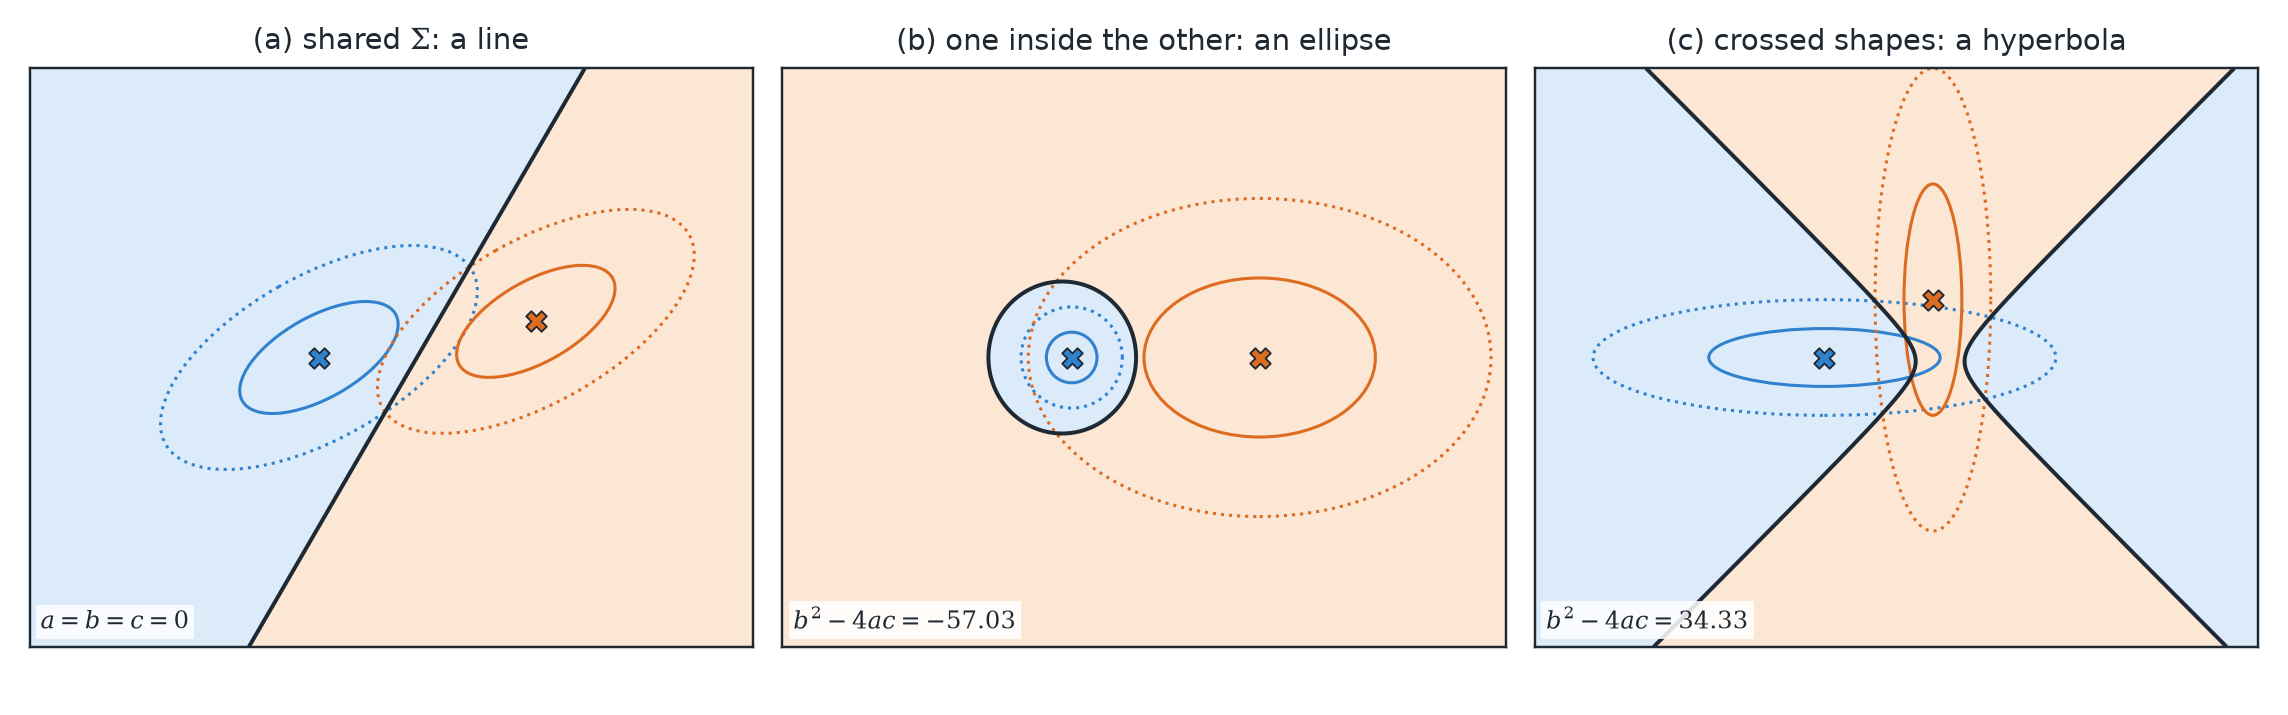
\includegraphics[width=\textwidth]{figures/gmm_conics.png}
\caption{The three kinds of GMM boundary, with equal weights. Ellipses are $1$ (solid) and $2$ (dotted) standard deviations; blue is where component $1$ wins. \emph{(a)} The same tilted covariance for both: the quadratic terms cancel, leaving a line. \emph{(b)} The example of Figure~\ref{fig:kmgmmbound}: the blue component is tighter in every direction, $b^2-4ac=-57.0$, and the boundary is an ellipse around it. \emph{(c)} Blue is wide and flat, orange tall and thin: $a=2.93$, $c=-2.93$, $b^2-4ac=34.3$, a hyperbola. Blue claims the far left and far right, orange the top and bottom.}
\label{fig:gmmconics}
\end{figure}

\textbf{Kernel $k$-means} works with $\varphi(\vx)$ in a feature space, as in Section~\ref{sec:kpca}, and uses $\norm{\varphi(\vx_i)-\varphi(\vx_j)}^2$ in place of the Euclidean distance. The center $\bm c_l=\frac1{|\mathcal C_l|}\sum_{j\in\mathcal C_l}\varphi(\vx_j)$ is never computed: the distance to it uses only the kernel matrix $K_{ij}=k(\vx_i,\vx_j)$:
\[
\norm{\varphi(\vx_i)-\bm c_l}^2=K_{ii}-\frac2{|\mathcal C_l|}\sum_{j\in\mathcal C_l}K_{ij}+\frac1{|\mathcal C_l|^2}\sum_{j,j'\in\mathcal C_l}K_{jj'} .
\]
It is just $\norm{\bm a-\bm b}^2=\bm a\T\bm a-2\bm a\T\bm b+\bm b\T\bm b$ with $\bm b$ the cluster's average, and each term reads in words: the point's similarity to itself, minus twice its \emph{average similarity to the cluster's members}, plus the cluster's average similarity among its own members (how tight it is). So a point belongs to the cluster whose members it resembles most, on average, after adjusting for how tight each cluster is.

Figure~\ref{fig:kkmterms} works through this for one point $\vx_i=(0.99,0)$ on the inner of two rings, with the RBF kernel $k(\vx,\vy)=e^{-\norm{\vx-\vy}^2/2\sigma^2}$, $\sigma=0.8$. $K_{ii}=1$ for every point, so the first term never decides anything. The point's average similarity is $0.40$ to the inner ring and $0.005$ to the outer ring, so the middle term is $-0.79$ against $-0.01$. The inner ring is tighter ($0.36$ against $0.12$), which counts against it, but not enough. The squared distances are $0.57$ to the inner ring's center and $1.11$ to the outer one's, so the point stays on the inner ring. Running the whole algorithm this way (best of $30$ random starts) recovers both rings exactly, and the boundary it draws in the plane is a closed curve between them.

\begin{figure}[htbp]
\centering
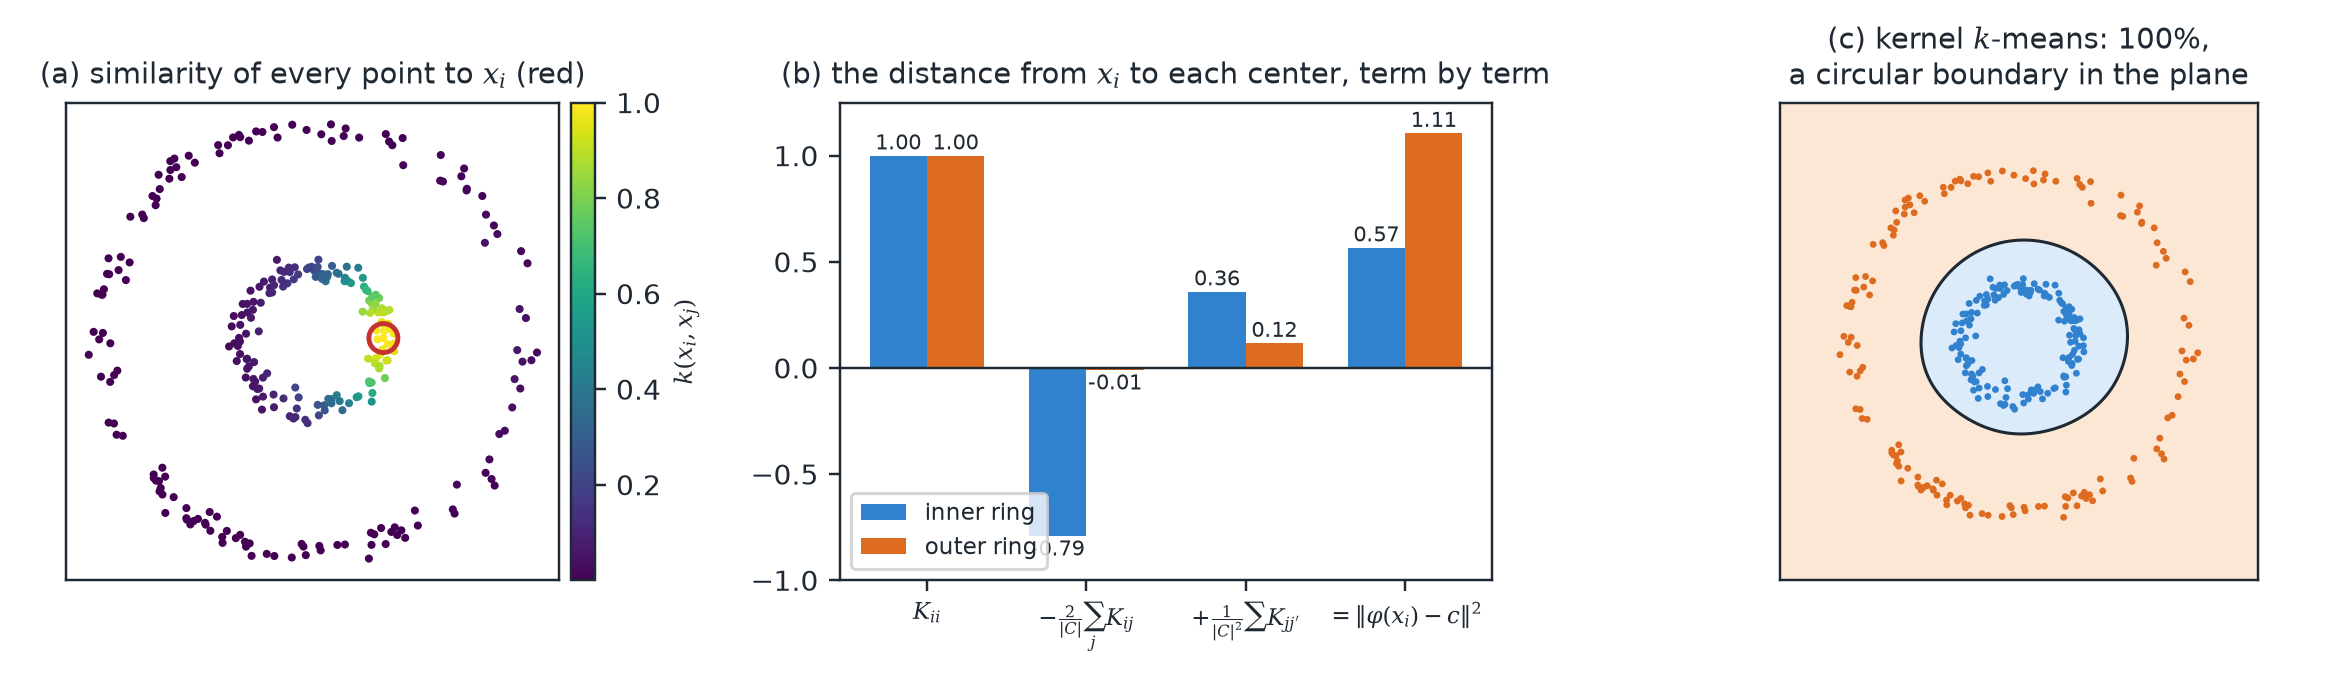
\includegraphics[width=\textwidth]{figures/kernel_kmeans_terms.png}
\caption{Kernel $k$-means with an RBF kernel ($\sigma=0.8$) on two rings. \emph{(a)} The similarity $k(\vx_i,\vx_j)$ of every point to one point $\vx_i$ (red circle). Only its neighbors on the inner ring are similar to it. \emph{(b)} The three terms of $\norm{\varphi(\vx_i)-\bm c}^2$ for each cluster. The middle term, the point's average similarity to the cluster, decides the outcome: $0.57$ to the inner ring against $1.11$ to the outer. \emph{(c)} The result is $100\%$ correct, and the region assigned to the inner ring is a disk, a curved boundary that ordinary $k$-means cannot draw.}
\label{fig:kkmterms}
\end{figure}
Straight cuts in feature space can be curved cuts in the original space. Panel (d) of Figure~\ref{fig:kmshapes} uses a related approach: it builds a neighbor graph, embeds it with Laplacian eigenmaps (Section~\ref{sec:laplacian}), and runs ordinary $k$-means on the embedding.

The simplest lift shows why kernels help (Figure~\ref{fig:kmlift}). With $\varphi(\vx)=(x_1,x_2,x_1^2+x_2^2)$, whose kernel is $k(\vx,\vy)=\vx\T\vy+\norm{\vx}^2\norm{\vy}^2$, each point rises to a height equal to its squared radius. The inner ring sits near height $1$ and the outer ring near $9$. Ordinary $k$-means on the lifted points (best of $10$ starts) recovers the two rings exactly, with centers at heights $1.05$ and $8.99$. The flat cut between them in $\R^3$ is a circle back in the plane.

\begin{figure}[htbp]
\centering
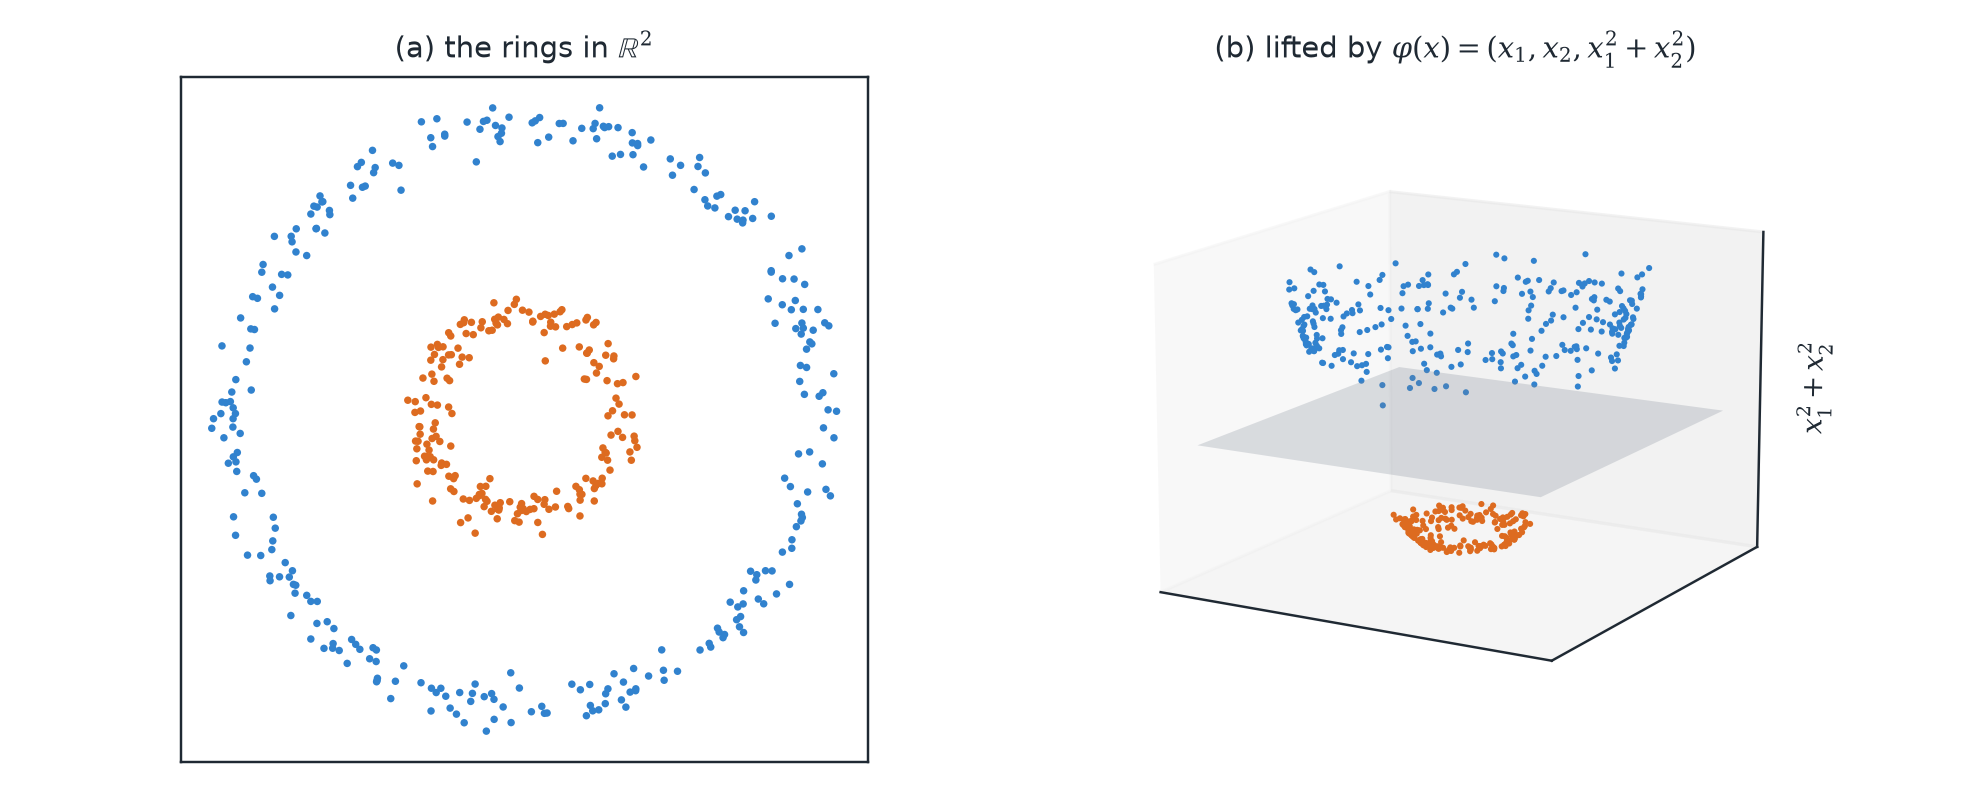
\includegraphics[width=0.9\textwidth]{figures/kmeans_lift.png}
\caption{The rings of Figure~\ref{fig:kmshapes}, colored by $k$-means run on the lifted points. In $\R^2$ no straight line separates the rings; in feature space a horizontal plane does, so the nearest-center rule now gets them $100\%$ right.}
\label{fig:kmlift}
\end{figure}

\subsection{Why not try every partition?}

For a fixed $k$, the obvious exact method is to compute $L$ for every partition and keep the best. The number of ways to split $N$ points into $k$ nonempty clusters is the \textbf{Stirling number of the second kind}:
\[
S(N,k)=\frac1{k!}\sum_{j=0}^{k}(-1)^{k-j}\binom kj\,j^N .
\]
There are $k^N$ ways to label the points; the alternating sum removes, by inclusion and exclusion, the labelings that leave some cluster empty; and $k!$ removes the order of the labels, which does not matter. For a small check, $S(4,2)=7$: four ways to split off one point and three ways to pair them up. The formula gets there in three moves. Label each of the $4$ points A or B: $2^4=16$ labelings. Two of them (all A, all B) leave a cluster empty, so $14$ remain. Swapping the names A and B gives the same partition, so divide by $2!$: $14/2=7$.
\[
S(10,4)=34{,}105,\qquad S(19,4)=11{,}259{,}666{,}950\approx1.1\times10^{10}.
\]
Nine extra points multiply the work by about $330{,}000$, and $S(N,k)$ grows like $k^N/k!$. Brute force is out of the question for real data.

\subsection{Lloyd's algorithm}

\begin{algorithm}{$k$-means (Lloyd's algorithm)}{lloyd}
\begin{enumerate}[nosep,label=\arabic*)]
\item \textbf{Initialize}, either (a) with $k$ random centers, or (b) with a random partition, then compute its centers.
\item \textbf{Assign} each point to its nearest center.
\item \textbf{Update} each center to the mean of its cluster, $\bm c_l=\frac1{|\mathcal C_l|}\sum_{\vx_i\in\mathcal C_l}\vx_i$.
\item Repeat steps 2--3 until the assignments stop changing.
\end{enumerate}
\end{algorithm}

\begin{proposition}{Lloyd's algorithm stops, at a local minimum}{lloydstops}
Neither step increases $L$, and the algorithm stops after finitely many steps.
\end{proposition}
\begin{proofsketch}
Think of $L$ as a function of both the partition and the centers, $\sum_l\sum_{\vx_i\in\mathcal C_l}\norm{\vx_i-\bm c_l}^2$. The assign step lowers or keeps each point's own term, since it picks the closest center. The update step lowers or keeps each cluster's term by Proposition~\ref{prop:pairwise}(b). So $L$ never goes up. There are finitely many partitions, and a partition cannot come back once $L$ has dropped below its value, so the assignments must stop changing.
\end{proofsketch}

\begin{intuition}
\textbf{Two easy problems instead of one hard one.} $L$ depends on two things: who belongs to which cluster, and where the centers are. Each is easy to optimize if the other is held fixed. Given the centers, the best assignment sends each point to its nearest center. Given the clusters, the best center is the mean, by Proposition~\ref{prop:pairwise}(b). Lloyd's algorithm alternates the two, like a town that keeps moving each post office to the middle of its customers, after which the customers switch to whichever office is now closest. Neither move can make the total walking distance worse. That is also why it can get stuck: when neither move helps on its own, the algorithm stops, even if moving several centers at once would help a lot.
\end{intuition}

\begin{figure}[htbp]
\centering
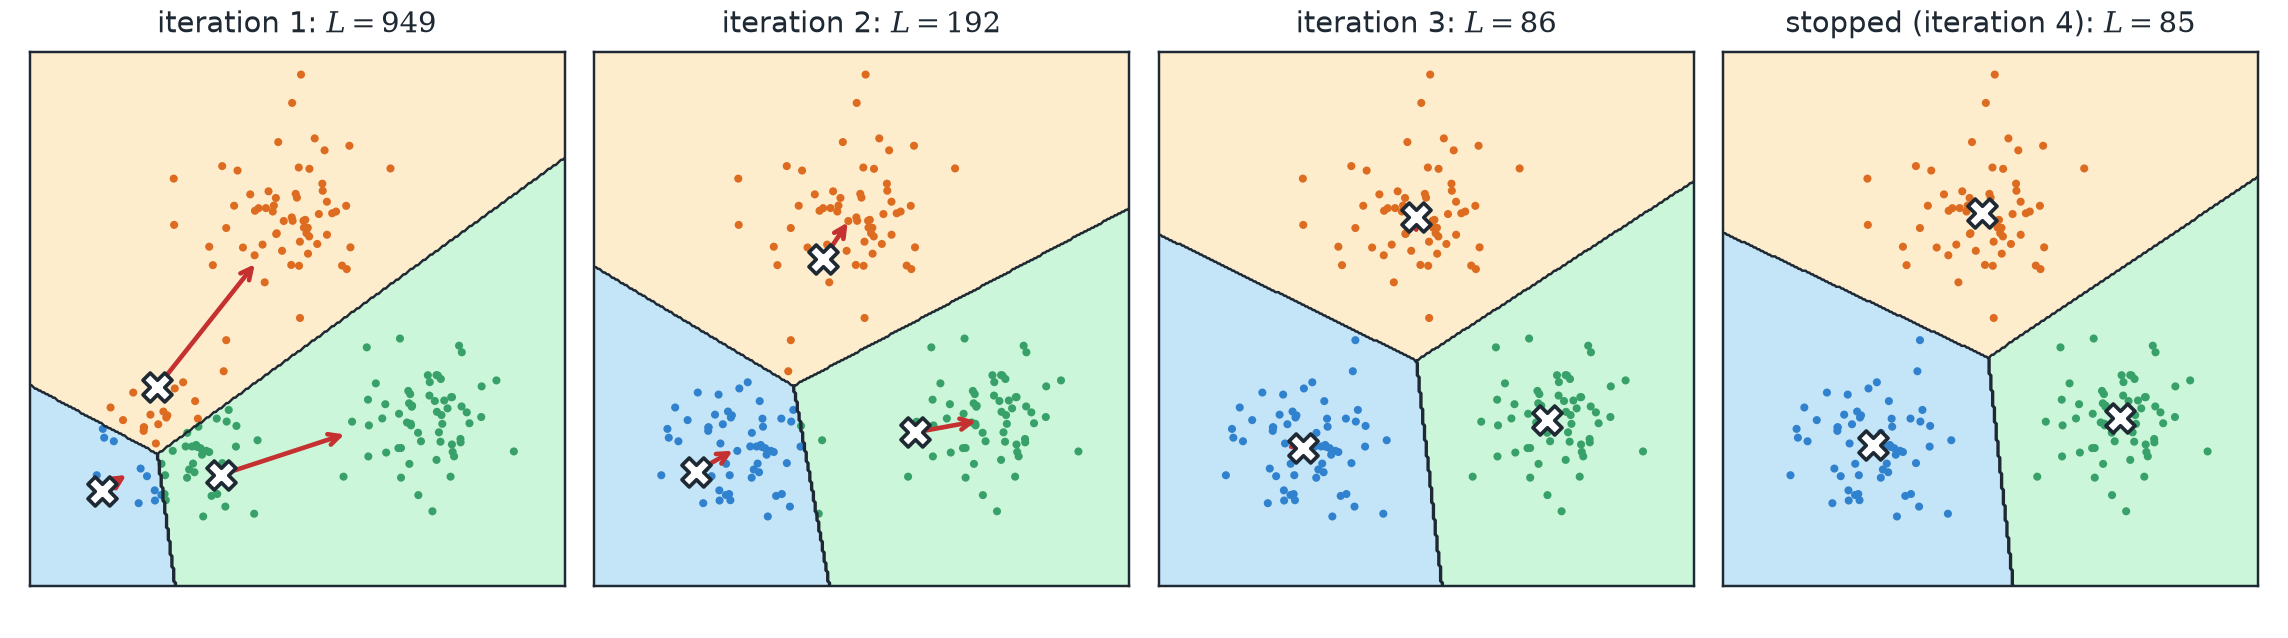
\includegraphics[width=\textwidth]{figures/kmeans_lloyd.png}
\caption{Lloyd's algorithm from a bad start, with all three centers in the lower-left group. \emph{Shading is the assign step:} each region is the set of locations nearest one center, so the boundaries are perpendicular bisectors between pairs of centers. \emph{Red arrows are the update step:} each center moves to the mean of the points it was assigned. The loss with the current centers falls $949\to192\to86\to85$, and then nothing changes. A start this bad still worked here; Example~\ref{ex:lloydstuck} shows one that does not.}
\label{fig:kmlloyd}
\end{figure}

\textbf{It is a greedy algorithm, and it is not optimal.} When it stops, no single assign or update step can lower $L$, but a better partition may still exist. That is a \emph{local} minimum.

\begin{example}{Lloyd's algorithm stuck far from the optimum}{lloydstuck}
Take four points, $(0,2)$, $(0,-2)$, $(3,\varepsilon)$ and $(3,-\varepsilon)$ with small $\varepsilon>0$, and $k=3$. Start the centers at $(3,\varepsilon)$, $(3,-\varepsilon)$ and $(0,0)$.
\begin{center}
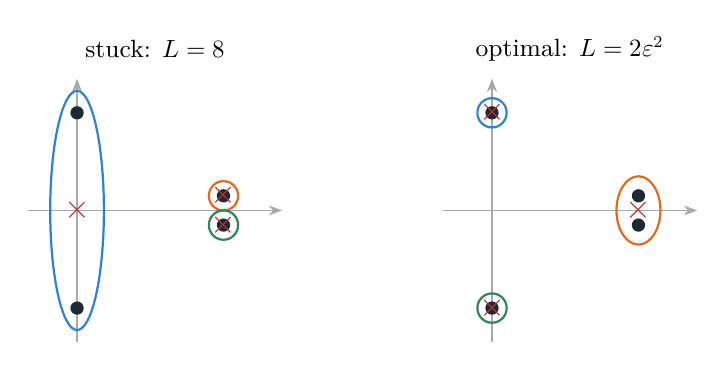
\begin{tikzpicture}[x=0.62cm,y=0.62cm,>=Stealth]
\foreach \dx/\ttl in {0/{stuck: $L=8$},8.5/{optimal: $L=2\varepsilon^2$}} {
  \begin{scope}[shift={(\dx,0)}]
  \draw[->,softgray!70!black] (-1,0) -- (4.2,0); \draw[->,softgray!70!black] (0,-2.7) -- (0,2.7);
  \node[font=\small] at (1.6,3.3) {\ttl};
  \end{scope}}
\draw[thick,dataC] (0,0) ellipse (0.55 and 2.45);
\draw[thick,accentC] (3,0.3) circle (0.3); \draw[thick,intgreen] (3,-0.3) circle (0.3);
\foreach \p in {(0,2),(0,-2),(3,0.3),(3,-0.3)} \fill[ink] \p circle (2.4pt);
\foreach \p in {(0,0),(3,0.3),(3,-0.3)} \node[font=\large,thmred] at \p {$\times$};
\begin{scope}[shift={(8.5,0)}]
\draw[thick,dataC] (0,2) circle (0.3); \draw[thick,intgreen] (0,-2) circle (0.3);
\draw[thick,accentC] (3,0) ellipse (0.45 and 0.7);
\foreach \p in {(0,2),(0,-2),(3,0.3),(3,-0.3)} \fill[ink] \p circle (2.4pt);
\foreach \p in {(0,2),(0,-2),(3,0)} \node[font=\large,thmred] at \p {$\times$};
\end{scope}
\end{tikzpicture}
\end{center}
\textbf{Assign:} each point at $x=3$ is its own center's only point. $(0,\pm2)$ are at distance $2$ from $(0,0)$ and more than $3$ from the other two centers, so both go to $(0,0)$. \textbf{Update:} the means are $(3,\varepsilon)$, $(3,-\varepsilon)$ and $(0,0)$, the same centers. Nothing changes, so the algorithm stops with
\[
L=\underbrace{2^2+2^2}_{(0,\pm2)\text{ around }(0,0)}+0+0=8 .
\]
The best partition puts each of $(0,\pm2)$ in a cluster of its own and pairs up the two close points, giving $L=\varepsilon^2+\varepsilon^2=2\varepsilon^2$. The ratio $8/(2\varepsilon^2)$ grows without bound as $\varepsilon\to0$, so a bad start can make Lloyd's algorithm arbitrarily far from optimal. The problem is two centers spent on two points that are almost on top of each other.
\end{example}

\textbf{$k$-means++ initialization.} Choose starting centers that are spread out, so two centers rarely start in the same cluster:
\begin{enumerate}[nosep]
\item pick the first center uniformly at random from the data;
\item pick each next center from the data at random, with probability proportional to $\mathrm{dist}(\vx_i)^2$, the squared distance from $\vx_i$ to the nearest center chosen so far;
\item when there are $k$ centers, run Lloyd's algorithm.
\end{enumerate}
In the example above, a point near an existing center gets almost no chance of being chosen, so the stuck start is very unlikely. On average, $k$-means++ alone is within a factor $O(\log k)$ of the optimal loss, before Lloyd's algorithm improves it further. Concretely, suppose the first center lands on $(3,\varepsilon)$. The squared distances to it are about $13$ for each of $(0,\pm2)$ and $4\varepsilon^2$ for $(3,-\varepsilon)$, so with $\varepsilon=0.01$ the second center is $(0,2)$ or $(0,-2)$ with probability about $0.50$ each, and $(3,-\varepsilon)$ with probability under $0.0001$. Say it is $(0,2)$. Now $(0,-2)$ is at squared distance $16$ from its nearest center and everything else is at $0$ or $4\varepsilon^2$, so the third center is $(0,-2)$ with probability $0.99997$. The start is then already the optimal partition.

\textbf{Why squared distance.} The weight $\mathrm{dist}(\vx_i)^2$ is exactly the amount $\vx_i$ would add to $L$ if the centers chosen so far were the final ones. So $k$-means++ places each new center, at random, where the current loss is concentrated.

\begin{careful}
\textbf{Not ``as far apart as possible.''} $k$-means++ is random, and it is only \emph{weighted} toward far points. Always taking the farthest remaining point (farthest-point initialization) is a different rule, and it tends to choose outliers as centers. Also, $k$-means++ improves the odds but does not guarantee the global minimum, so multiple starts are still worthwhile.
\end{careful}

\begin{figure}[htbp]
\centering
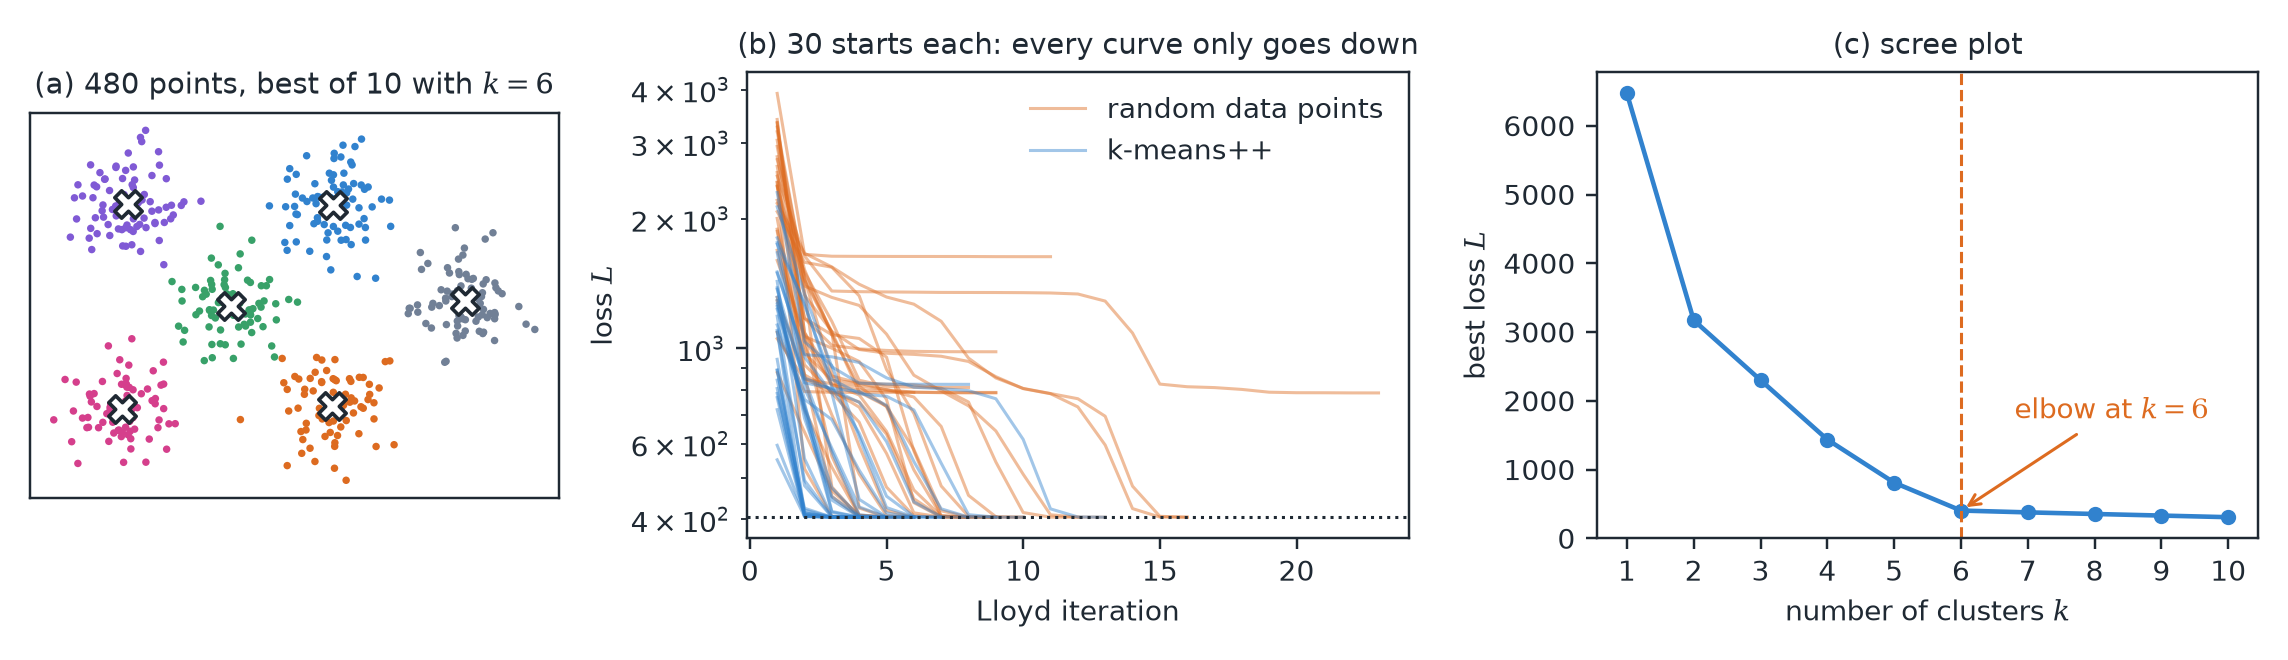
\includegraphics[width=\textwidth]{figures/kmeans_starts.png}
\caption{\emph{(a)} $480$ points in six groups. \emph{(b)} Thirty runs of Lloyd's algorithm from random data points (orange) and thirty from $k$-means++ (blue), with $k=6$. Every curve goes down and then stops, as Proposition~\ref{prop:lloydstops} says, but not all at the same level. The best loss is $404.7$ (dotted line). $23$ of $30$ random starts reach it, and the worst stops at $1634.2$. $29$ of $30$ $k$-means++ starts reach it, and the worst stops at $824.6$. $k$-means++ also needs fewer iterations (median $5$ against $8$). \emph{(c)} The best loss over $10$ starts for $k=1,\dots,10$: $6470,\,3172,\,2302,\,1437,\,811,\,405$, and then only $378,\,355,\,332,\,308$.}
\label{fig:kmstarts}
\end{figure}

\textbf{In practice:}
\begin{enumerate}[nosep]
\item initialize with $k$-means++;
\item run Lloyd's algorithm from several random starts;
\item keep the partition with the lowest within-cluster variation $L$.
\end{enumerate}

\textbf{Choosing $k$.} You cannot simply pick the $k$ with the lowest $L$. The best loss always goes down as $k$ grows (one more center can always split a cluster), and it reaches $0$ at $k=N$, with every point its own cluster. Instead, plot the best $L$ against $k$, which is a \textbf{scree plot} like the one for PCA, and look for the \textbf{elbow}, where adding clusters stops helping much. In Figure~\ref{fig:kmstarts}(c), going from $5$ to $6$ clusters halves the loss ($811\to405$), and each later step saves only about $6$--$7\%$, so $k=6$. On real data the elbow is often less clear than this.

\subsection{Choosing $k$ beyond the elbow}

The elbow is one of three standard ways to choose $k$, or more generally to judge how good a clustering is. The other two, the \textbf{gap statistic} and \textbf{silhouette scores}, also work for clustering algorithms other than $k$-means.

\subsubsection*{The gap statistic: is the clustering tighter than chance?}

$L$ falls as $k$ grows for \emph{any} data, even data with no clusters at all. So the question is not whether $L_{\mathrm{data}}(k)$ is small, but whether it is smaller than clustering would achieve on data with no structure. The gap statistic manufactures such data and compares.

\begin{algorithm}{The gap statistic (Tibshirani, Walther \& Hastie)}{gap}
For $k=1,\dots,K$:
\begin{enumerate}[nosep,label=\arabic*)]
\item Cluster the data into $k$ clusters and record $L_{\mathrm{data}}(k)$, the minimal within-cluster variation.
\item For $b=1,\dots,B$ (typically $B$ is $50$ to $1000$): draw $N$ points uniformly from the box that bounds the data (each coordinate from its own minimum to maximum), cluster them into $k$ clusters, and record $L^{*}_b(k)$.
\item Compute
\[
\mathrm{Gap}(k)=\frac1B\sum_{b=1}^B\log L^{*}_b(k)\;-\;\log L_{\mathrm{data}}(k),
\qquad s_k=\mathrm{sd}_b\big(\log L^{*}_b(k)\big)\sqrt{1+1/B}.
\]
\end{enumerate}
Choose the \textbf{smallest} $k$ with $\ \mathrm{Gap}(k)\ \ge\ \mathrm{Gap}(k+1)-s_{k+1}$.
\end{algorithm}

\textbf{Why logs.} A difference of logs is the log of a ratio, so the gap compares the data's within-cluster variation to the reference's as a ratio. In Figure~\ref{fig:gap}, $\mathrm{Gap}(3)=1.45$: at $k=3$ the real data's within-cluster variation is about $e^{1.45}\approx4.3$ times smaller than for uniform data (in the geometric-mean sense). A large gap means the clustering is meaningfully tighter than chance.

\textbf{Why the rule.} Read it as: \emph{stop at the first $k$ where one more cluster does not raise the gap by more than the noise.} $s_{k+1}$ is the standard error of the simulated term (the lecture writes it $\widehat\sigma_{k+1}$). The extra factor $\sqrt{1+1/B}$ in the original paper accounts for the simulation error of the reference average, and it is close to $1$ when $B$ is large. Your notes mention an alternative, simply taking the $k$ with the largest gap. Figure~\ref{fig:gap}(d) shows the risk: on uniform data, the largest gap is at $k=8$ ($0.038$), which is pure noise, while the rule correctly stops at $k=1$.

\begin{intuition}
\textbf{What the two curves look like.} Without clusters, $\log L$ falls smoothly. On a uniform interval, $k$ equal pieces each have variance proportional to $(1/k)^2$, so $L^*\propto k^{-2}$, and in $d$ dimensions $L^*\propto k^{-2/d}$ for large $k$. Each extra center buys about the same small, predictable improvement. With real clusters, the curve drops sharply while each extra center separates a genuine group, because a center that moves from \emph{between} two groups to \emph{inside} one removes the large gap between them from the loss. Once each group has its own center, extra centers only chop groups into pieces, and the real data's curve falls at the same smooth rate as the reference's. The gap is the vertical distance between the two curves, so it climbs during the sharp drops and then levels off, and the rule stops where it levels off.
\end{intuition}

\begin{figure}[htbp]
\centering
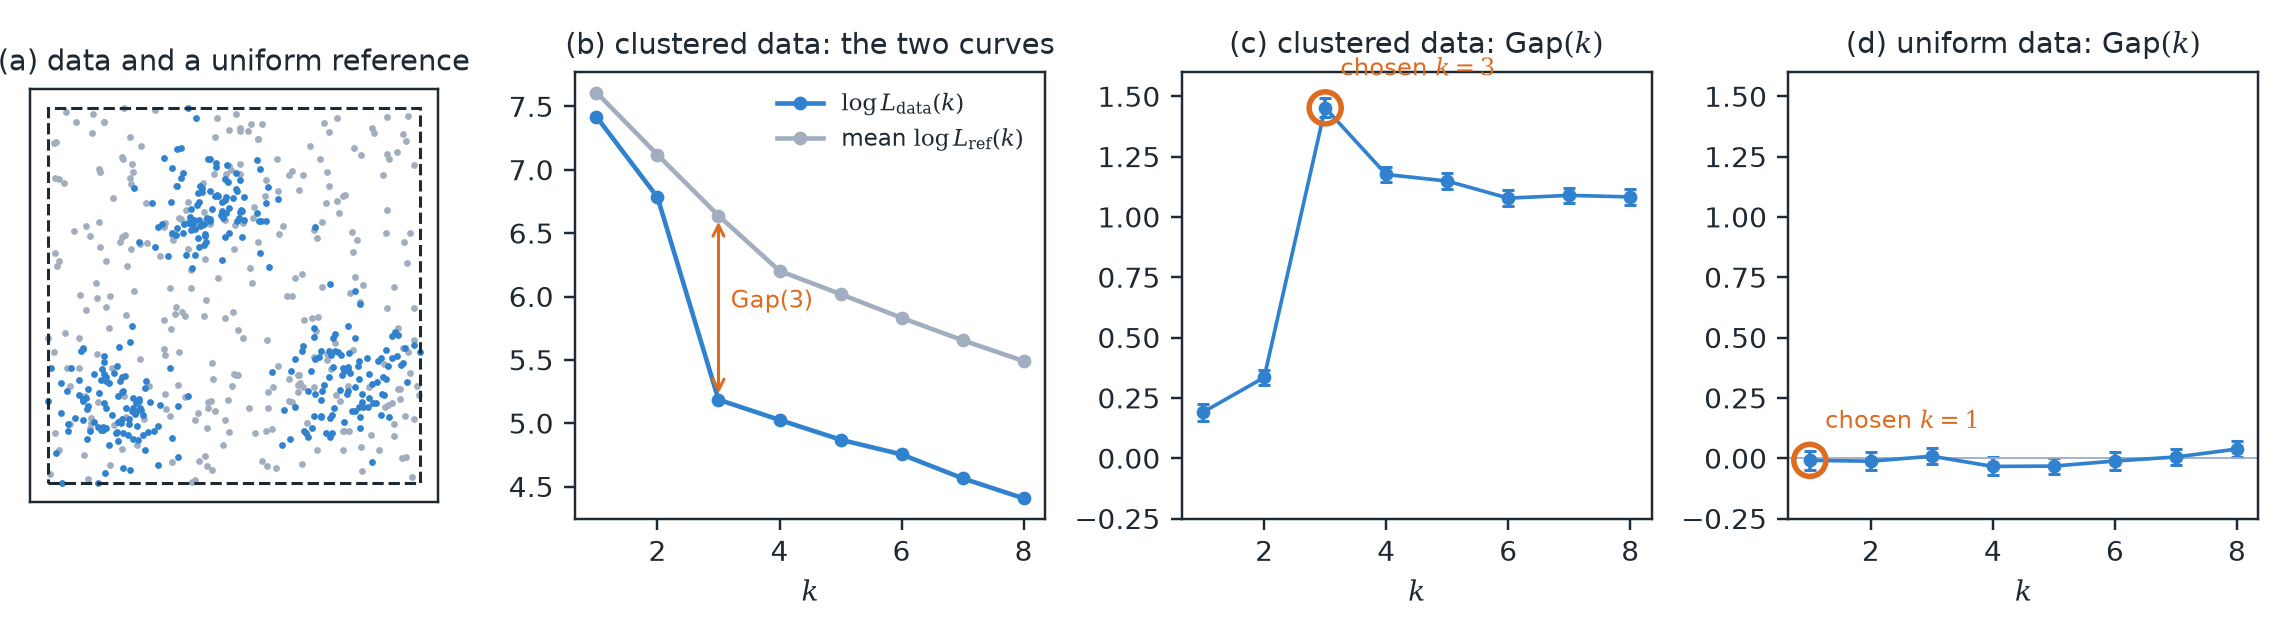
\includegraphics[width=\textwidth]{figures/gap_stat.png}
\caption{The gap statistic with $k$-means, $B=50$. \emph{(a)} $300$ points in three groups (blue) and one uniform reference set drawn from their bounding box (gray). \emph{(b)} Both curves fall with $k$, but the data's drops much faster up to $k=3$. \emph{(c)} $\mathrm{Gap}(k)=0.19,\,0.34,\,1.45$, then between $1.08$ and $1.18$, with error bars $\pm s_k$; the rule picks $k=3$. \emph{(d)} $300$ uniform points: every gap is within noise of $0$ (from $-0.034$ to $0.038$), and the rule picks $k=1$, ``no clusters.''}
\label{fig:gap}
\end{figure}

\begin{careful}
\begin{itemize}[nosep,leftmargin=*]
\item \textbf{It can say $k=1$.} The gap can conclude that the data have no cluster structure at all, as in panel (d). The elbow cannot really say this, and silhouettes cannot even be computed at $k=1$.
\item \textbf{Same objective for every method being compared.} The gap was developed with $L$, the $k$-means objective, as the measure, which makes it a fair way to compare $k$-means at different $k$. It can also compare \emph{different algorithms}, but only if one measure is applied to all of them. Scoring every algorithm with $L$ favors $k$-means, since $k$-means is exactly the method that minimizes $L$.
\item \textbf{The most expensive of the three.} It reruns the clustering for every $k$ on the data and on every reference set: $(B+1)K$ clusterings, each with several starts. Figure~\ref{fig:gap} used $51\times8=408$ runs per dataset.
\item \textbf{The reference is a choice.} An axis-aligned box fits a tilted, elongated cloud poorly. The original paper also suggests a box aligned with the data's principal components.
\end{itemize}
\end{careful}

\subsubsection*{Silhouette scores: how well does each point fit its cluster?}

\begin{definition}{Silhouette}{silhouette}
For a point $\vx_i$ in cluster $\mathcal C$:
\begin{itemize}[nosep]
\item $a_i$ is the average distance from $\vx_i$ to the \emph{other} points of $\mathcal C$;
\item $b_i$ is the smallest, over every other cluster $\mathcal C'$, of the average distance from $\vx_i$ to the points of $\mathcal C'$ (the nearest rival cluster);
\item $s_i=\dfrac{b_i-a_i}{\max(a_i,b_i)}\in[-1,1]$, with $s_i=0$ if $\vx_i$ is alone in its cluster.
\end{itemize}
\end{definition}

\begin{center}
\small
\renewcommand{\arraystretch}{1.2}
\begin{tabular}{@{}lll@{}}
\toprule
$s_i$ & Meaning & Why\\
\midrule
near $+1$ & well clustered & $a_i\ll b_i$: much closer to its own cluster than to any other\\
near $0$ & on a boundary & $a_i\approx b_i$\\
negative & probably in the wrong cluster & $a_i>b_i$: closer, on average, to another cluster's points\\
\bottomrule
\end{tabular}
\end{center}

A \textbf{silhouette plot} draws one horizontal bar of length $s_i$ per point, grouped by cluster and sorted within each group. It shows at a glance which clusters are tight and which are poorly separated. To choose $k$, cluster for each $k$, compute the mean silhouette, and pick the $k$ where it is highest.

\begin{intuition}
\textbf{Stay or move?} Ask each point: would you rather stay in your cluster, or move to the nearest other one? $a_i$ is the cost of staying and $b_i$ the cost of moving, both measured as average distance. $s_i$ is the saving from staying as a fraction of the larger cost, so it has no units and lies in $[-1,1]$. For example, $a_i=1$ and $b_i=4$ give $s_i=3/4$: staying saves three quarters of the distance. When $a_i>b_i$ the point would rather move, and $s_i<0$.
\end{intuition}

\begin{figure}[htbp]
\centering
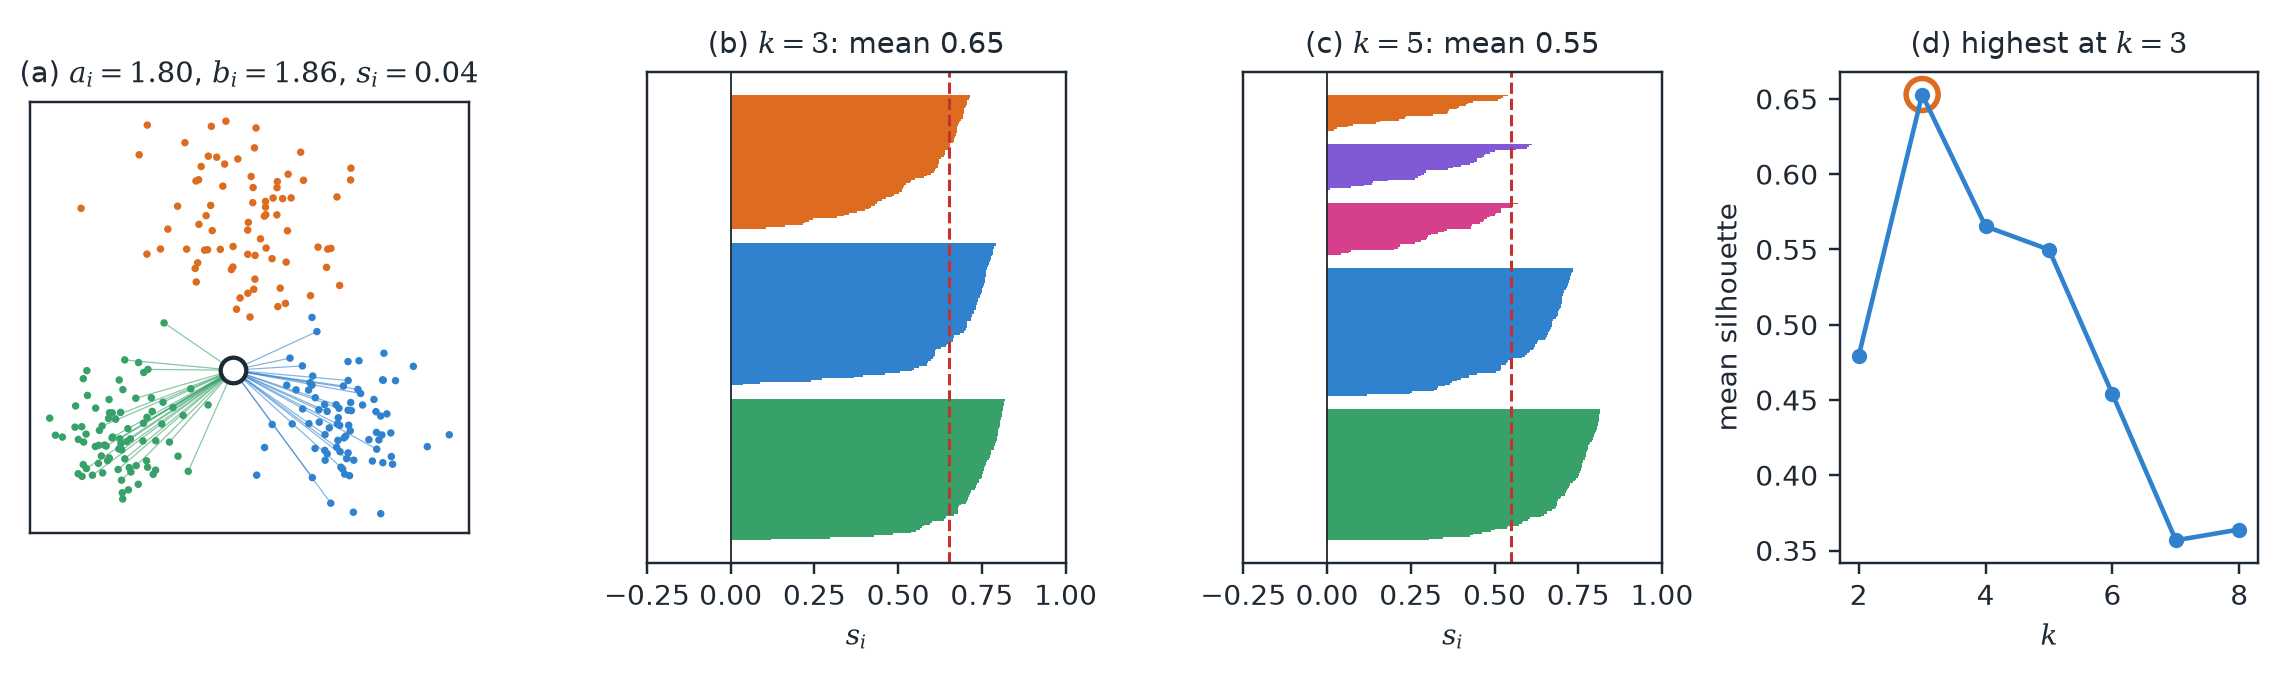
\includegraphics[width=\textwidth]{figures/silhouette.png}
\caption{Silhouettes for $k$-means on $240$ points in three groups. \emph{(a)} One point between two groups. Its average distance to its own (blue) cluster is $a_i=1.80$ and to the nearest rival (green) is $b_i=1.86$, so $s_i=0.04$: it is on the boundary. \emph{(b)} $k=3$: every bar is long, and the mean is $0.65$ (red line). \emph{(c)} $k=5$ splits the loose orange group into three pieces. Their bars are shorter, because each piece's nearest rival is a sibling right next to it. The mean falls to $0.55$. \emph{(d)} The mean silhouette for $k=2,\dots,8$ is $0.48,\,0.65,\,0.57,\,0.55,\,0.45,\,0.36,\,0.36$, highest at $k=3$.}
\label{fig:silhouette}
\end{figure}

\begin{careful}
\begin{itemize}[nosep,leftmargin=*]
\item \textbf{Average distances, not centers.} A negative $s_i$ means the point is closer \emph{on average} to the points of another cluster. It does not mean closer to another cluster's center; no centers appear in the definition, so silhouettes work for any clustering.
\item \textbf{Biases.} With Euclidean distance, silhouettes favor compact, round, well-separated clusters, the same shapes $k$-means likes, so on rings or long clusters they reward the wrong answer. The metric can be swapped for one that suits the data.
\item \textbf{Not defined at $k=1$,} since $b_i$ needs a second cluster, and computing all the pairwise distances costs $O(N^2)$.
\end{itemize}
\end{careful}

\subsection{Model-based clustering: Gaussian mixture models}

\textbf{What goes wrong with $k$-means.}
\begin{itemize}[nosep]
\item \textbf{Outliers.} Squared distances let one far point dominate, and a mean is easily dragged: the mean of $0,1,2,30$ is $8.25$, nowhere near three of the four points.
\item \textbf{Round clusters only.} Every cluster is a convex cell cut by perpendicular bisectors, so elongated or tilted clusters are cut the wrong way (Figure~\ref{fig:kmshapes}(b)).
\item \textbf{Spread is ignored.} A point is assigned purely by distance to the nearest center. A point halfway between a tight cluster and a broad one is more plausibly from the broad one, but $k$-means cannot tell.
\item \textbf{Hard answers only.} Every point gets one label, with no statement of uncertainty.
\end{itemize}

\textbf{A probabilistic view of clustering.} Instead of a loss, write down a model of how the data were generated, fit it, and read the clusters off the fitted model.

\begin{definition}{Mixture model}{mixture}
Fix densities $f_1(\vx),\dots,f_k(\vx)$ on $\R^d$ and probabilities $p_1,\dots,p_k>0$ with $\sum_jp_j=1$. The data $\vx_1,\dots,\vx_N$ are i.i.d.\ draws from a two-step process:
\begin{enumerate}[nosep,label=(\roman*)]
\item draw a cluster label $z_i\in\{1,\dots,k\}$, with $z_i=j$ with probability $p_j$;
\item given $z_i=j$, draw $\vx_i\mid z_i=j\ \sim\ f_j$.
\end{enumerate}
Equivalently, the $\vx_i$ are i.i.d.\ draws from the \textbf{mixture density}
\[
f_{\mathrm{mix}}(\vx)=\sum_{j=1}^kp_j\,f_j(\vx).
\]
\end{definition}
The two descriptions agree by the law of total probability: the density of $\vx_i$ is $\sum_jP(z_i=j)\,f(\vx\mid z_i=j)=\sum_jp_jf_j(\vx)$. The labels $z_i$ are \textbf{latent}: they generated the data, but we never see them. Clustering means recovering them.

\begin{figure}[htbp]
\centering
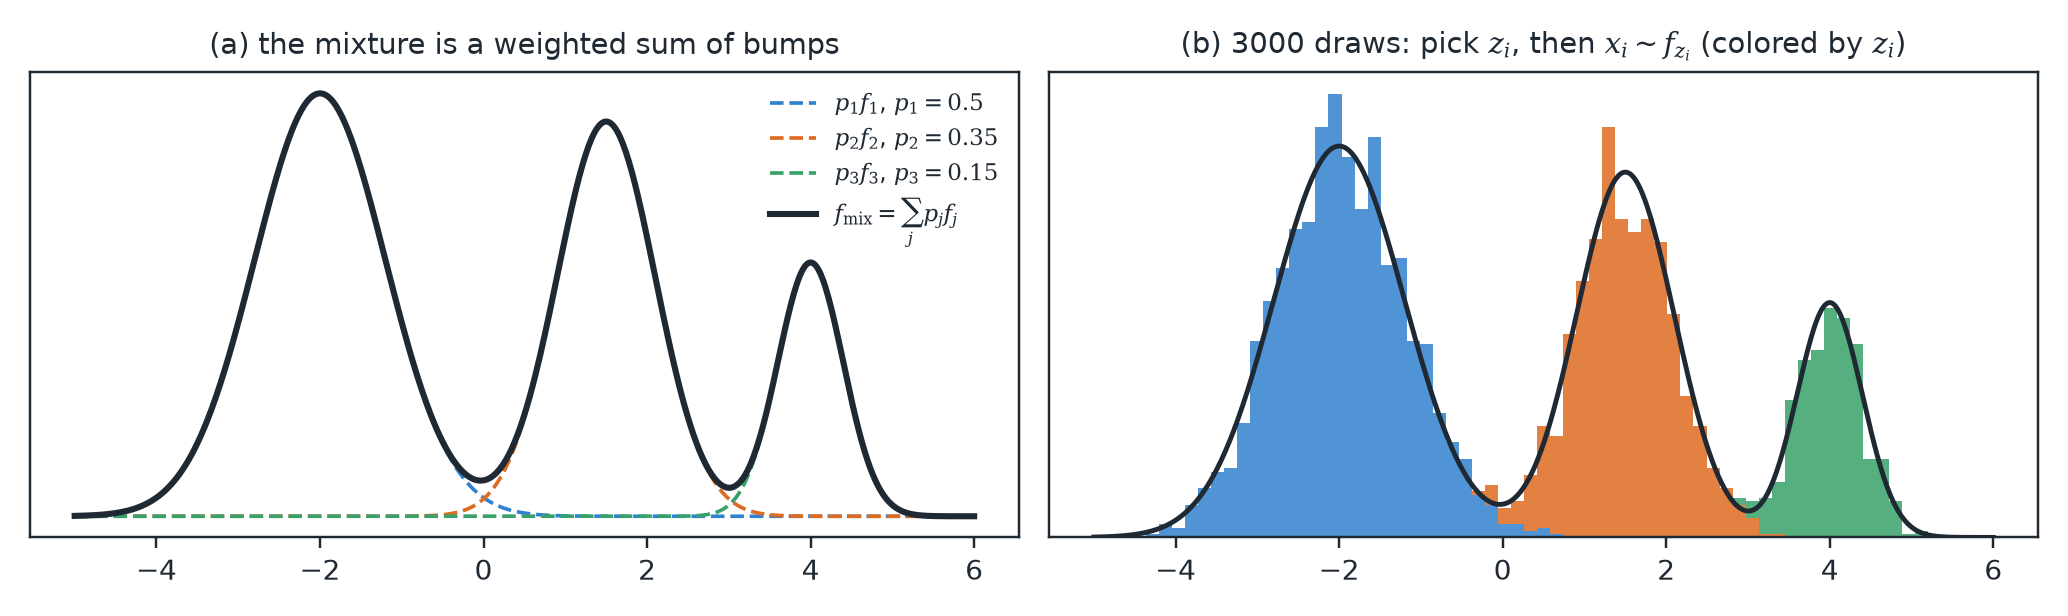
\includegraphics[width=0.95\textwidth]{figures/gmm_mixture.png}
\caption{A one-dimensional mixture of three Gaussians with $p=(0.5,0.35,0.15)$, like the sketch on the board. \emph{(a)} Each dashed curve is one weighted component $p_jf_j$, and $f_{\mathrm{mix}}$ is their sum, so it integrates to $\sum_jp_j=1$. \emph{(b)} $3000$ draws by the two-step process, colored by their label $z_i$ (in practice the colors are hidden). The fractions with each label are $0.51$, $0.34$ and $0.15$, and the histogram follows $f_{\mathrm{mix}}$.}
\label{fig:gmmmix}
\end{figure}

\textbf{The Gaussian mixture model (GMM).} Take each $f_j$ to be a multivariate Gaussian with its own mean $\bm\mu_j$ and covariance $\Sigma_j$:
\[
f_{\mathrm{mix}}(\vx)=\sum_{j=1}^k\frac{p_j}{(2\pi)^{d/2}\,|\Sigma_j|^{1/2}}\exp\!\Big(-\tfrac12(\vx-\bm\mu_j)\T\Sigma_j^{-1}(\vx-\bm\mu_j)\Big)=\sum_{j=1}^kp_j\,\mathcal N(\vx;\bm\mu_j,\Sigma_j).
\]
Each component's level sets are ellipsoids, with axes along the eigenvectors of $\Sigma_j$ and half-lengths proportional to the square roots of its eigenvalues, the same geometry as PCA. Relaxing $k$-means' round clusters to ellipsoids lets a cluster be long, thin and tilted.

\begin{intuition}
\textbf{Distance, squared distance, and Mahalanobis distance.} For $\vx=(5,5)$, the distance from the origin is $\norm{\vx}=\sqrt{5^2+5^2}=\sqrt{50}\approx7.07$, and $\vx\T\vx=50$ is the \emph{squared} distance. Gaussian densities and the $k$-means loss both use squared distances, because the density contains $\exp(-\frac12\cdot\text{squared distance})$.

The quantity in a Gaussian is the covariance-adjusted version, $\vx\T\Sigma^{-1}\vx$, the \textbf{squared Mahalanobis distance} (here from the mean $\bm0$). With $\Sigma=\begin{bmatrix}100&0\\0&1\end{bmatrix}$, $\Sigma^{-1}=\begin{bmatrix}1/100&0\\0&1\end{bmatrix}$ and
\[
\Sigma^{-1}\vx=\begin{bmatrix}0.05\\5\end{bmatrix},\qquad \vx\T\Sigma^{-1}\vx=5(0.05)+5(5)=0.25+25=25.25,
\]
so the Mahalanobis distance is $\sqrt{25.25}\approx5.02$. Read the two terms in standard deviations. Along $x_1$ the standard deviation is $10$, so $5$ is half a standard deviation and contributes $0.5^2=0.25$. Along $x_2$ it is $1$, so $5$ is five standard deviations and contributes $25$. The point is unusual because of $x_2$ alone. Points with the same Mahalanobis distance form an ellipse, here $10$ times longer along $x_1$ than along $x_2$: these are the level sets of the Gaussian.
\end{intuition}

\begin{careful}
\textbf{The weight $p_j$ multiplies the density.} The board writes $\dfrac1{p_j(2\pi)^{d/2}|\Sigma_j|^{1/2}}$, with $p_j$ in the denominator. It belongs in the numerator. Check by integrating: each Gaussian integrates to $1$, so $\int f_{\mathrm{mix}}=\sum_jp_j=1$, while with $p_j$ downstairs the total would be $\sum_j1/p_j$, which is at least $k^2$ and so exceeds $1$ whenever $k\ge2$.
\end{careful}

\textbf{Fitting, then assigning.} Collect the parameters as $\phi=\{p_j,\bm\mu_j,\Sigma_j\}_{j=1}^k$ and maximize the log-likelihood
\[
\ell(\phi)=\sum_{i=1}^N\log\sum_{j=1}^kp_j\,\mathcal N(\vx_i;\bm\mu_j,\Sigma_j).
\]
With the fitted $\widehat\phi$, Bayes' rule gives each point's \textbf{responsibilities}, the probability that it came from each component:
\[
r_{ij}=P(z_i=j\mid\vx_i,\widehat\phi)=\frac{p_j\,\mathcal N(\vx_i;\bm\mu_j,\Sigma_j)}{\sum_{l=1}^kp_l\,\mathcal N(\vx_i;\bm\mu_l,\Sigma_l)} .
\]
The hard label is $\arg\max_jr_{ij}$, but the $r_{ij}$ themselves are a \textbf{soft clustering}, and they answer two of the complaints above: assignment uses each cluster's spread through $\Sigma_j$, and every point comes with its uncertainty.

\begin{example}{The point halfway between a tight cluster and a broad one}{tightbroad}
In one dimension, take two equally likely components, a tight one $\mathcal N(0,0.5^2)$ and a broad one $\mathcal N(4,2^2)$, and the point $x=2$, exactly halfway between the means. $k$-means calls it a tie. But $x=2$ is $4$ standard deviations from the tight mean and only $1$ from the broad mean, so the densities are $\mathcal N(2;0,0.5^2)\approx0.00027$ and $\mathcal N(2;4,2^2)\approx0.121$, and
\[
r_{\text{broad}}=\frac{0.5\times0.121}{0.5\times0.00027+0.5\times0.121}\approx0.998 .
\]
Responsibilities measure distance in units of each component's own spread. A tight cluster ``claims'' only points very near it, and a broad one claims points far away. Even at $x=1.5$, closer to the tight mean, the broad component gets $r\approx0.91$.
\end{example}

\textbf{Expectation--maximization (EM).} The key insight: if the labels were known, the maximum-likelihood estimates would be easy, one cluster at a time. $p_j$ would be the fraction of points in cluster $j$, $\bm\mu_j$ its sample mean, and $\Sigma_j$ its sample covariance. EM replaces the unknown $0/1$ labels with responsibilities and alternates.

\begin{algorithm}{EM for a Gaussian mixture}{em}
Start from some $\phi$ (for example, $k$-means centers with round covariances). Repeat until $\ell(\phi)$ stops increasing:
\begin{enumerate}[nosep,label=\arabic*)]
\item \textbf{E-step:} compute $r_{ij}=P(z_i=j\mid\vx_i,\phi)$ for all $i,j$ with the current $\phi$.
\item \textbf{M-step:} with $N_j=\sum_ir_{ij}$, set the weighted versions of the known-label estimates:
\[
p_j=\frac{N_j}N,\qquad \bm\mu_j=\frac1{N_j}\sum_ir_{ij}\vx_i,\qquad \Sigma_j=\frac1{N_j}\sum_ir_{ij}(\vx_i-\bm\mu_j)(\vx_i-\bm\mu_j)\T .
\]
\end{enumerate}
\end{algorithm}

The M-step maximizes the expected complete-data log-likelihood, and each round never decreases $\ell$ (both are derived in Section~\ref{sec:emderiv}). So, like Lloyd's algorithm, EM climbs to a \emph{local} optimum, and the start matters. It is in fact a soft version of Lloyd's algorithm. Fix every $\Sigma_j=\sigma^2I$ and every $p_j=1/k$; then $r_{ij}\propto e^{-\norm{\vx_i-\bm\mu_j}^2/2\sigma^2}$, and as $\sigma\to0$ each point's responsibility goes entirely to its nearest center. The E-step becomes the assign step, and the M-step becomes the update step.

\begin{intuition}
\textbf{Soft counting.} Picture each point split into fractions, giving $r_{ij}$ of itself to component $j$. Then $N_j$ is how many points component $j$ owns in total, possibly fractional, and the M-step is the ordinary known-label estimates computed with fractional points. For example, if the points $0$, $2$ and $10$ give component A the fractions $1$, $0.5$ and $0$, then A owns $N_A=1.5$ points, $p_A=1.5/3=0.5$, and $\mu_A=(1\cdot0+0.5\cdot2)/1.5\approx0.67$. The E-step re-divides each point using the new parameters, and the two steps feed each other.
\end{intuition}

\begin{figure}[htbp]
\centering
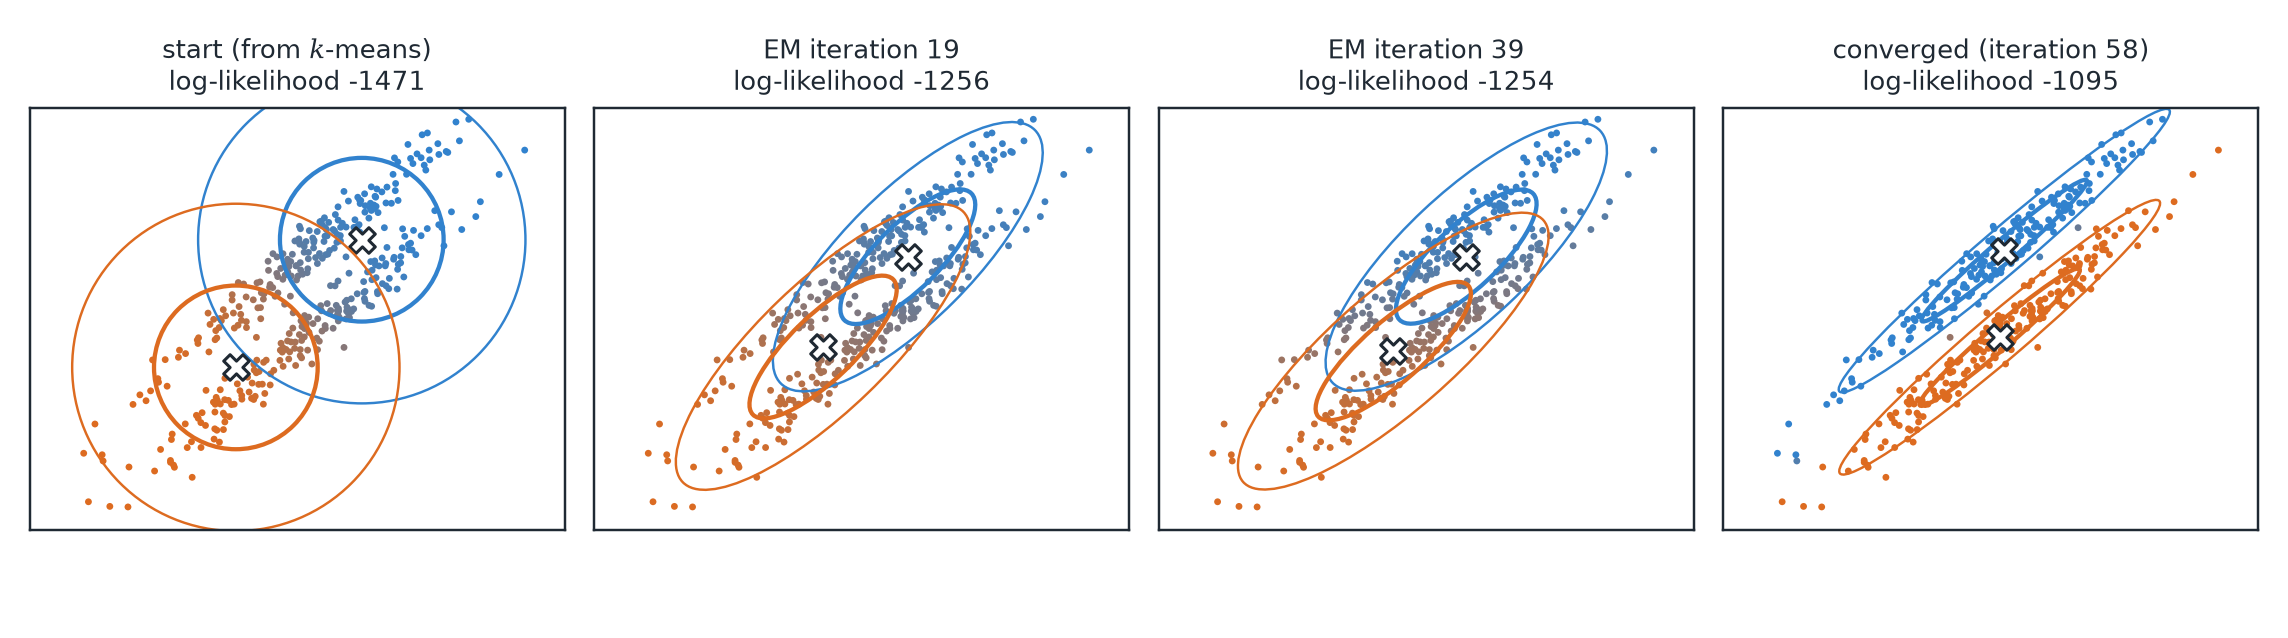
\includegraphics[width=\textwidth]{figures/gmm_em.png}
\caption{EM on the two long, parallel clusters that $k$-means cut across in Figure~\ref{fig:kmshapes}(b). Ellipses are $1$ and $2$ standard deviations of each component, and each point is colored by its responsibilities (a mix of blue and orange shows uncertainty). EM starts from the $k$-means answer with round covariances. The log-likelihood rises from $-1471$ to about $-1256$ within three iterations, creeps along for dozens more while the components sit on top of each other, and then the two ellipses slide apart, converging at $-1095$ after $58$ iterations. The log-likelihood never decreased. Hard labels match the true groups for $99.5\%$ of points, against $62.5\%$ for $k$-means.}
\label{fig:gmmem}
\end{figure}

\begin{careful}
\begin{itemize}[nosep,leftmargin=*]
\item \textbf{The likelihood has no maximum.} Put one $\bm\mu_j$ exactly on a data point and shrink $\Sigma_j\to0$: that component's density at the point goes to infinity, so $\ell\to\infty$. This degenerate ``solution'' is useless, so implementations add a small ridge to each $\Sigma_j$ (the figure's code adds $10^{-6}I$) or restart when a component collapses. ``The MLE'' really means a good local maximum.
\item \textbf{Starts matter here too.} On the same data, scikit-learn's default (which starts EM from $k$-means) found only poor two-component fits, with BIC $2578$. Twenty random starts found the right one, with BIC $2256$.
\end{itemize}
\end{careful}

\subsubsection{Deriving EM}\label{sec:emderiv}

The lecture writes the responsibilities at step $t$ as $T_{ij}^{(t)}$ (so $T_{ij}^{(t)}=r_{ij}$ computed from $\phi^{(t)}$). The goal is $\widehat\phi=\arg\max_\phi\log L(\phi\mid\vx_1,\dots,\vx_N)$, where $L(\phi\mid X)=\prod_i\sum_jp_j\,\mathcal N(\vx_i;\bm\mu_j,\Sigma_j)$ is the \textbf{observed-data likelihood}.

\textbf{Step 0: pretend the labels are known.} If we also saw $z_1,\dots,z_N$, the \textbf{complete-data likelihood} would be
\[
L(\phi\mid X,Z)=\prod_{i=1}^N\prod_{j=1}^k\big[p_j\,\mathcal N(\vx_i;\bm\mu_j,\Sigma_j)\big]^{\mathbb 1(z_i=j)} .
\]
For each $i$ exactly one indicator is $1$, so the inner product just picks out one factor,
\[
p_{z_i}\,\mathcal N(\vx_i;\bm\mu_{z_i},\Sigma_{z_i})=P(z_i)\,f(\vx_i\mid z_i).
\]
Its log is
\[
\log L(\phi\mid X,Z)=\sum_{i=1}^N\sum_{j=1}^k\mathbb 1(z_i=j)\,\log\big(p_j\,\mathcal N(\vx_i;\bm\mu_j,\Sigma_j)\big),
\]
a sum of logs, which splits cluster by cluster. The observed-data $\ell$ is a sum of logs \emph{of sums}, which does not. That is the whole difficulty, and EM gets around it by averaging over the labels it cannot see.

\textbf{E-step: a distribution over the missing labels.} Fix the current estimate $\phi^{(t)}$. By Bayes' rule,
\[
T_{ij}^{(t)}=P(z_i=j\mid\vx_i,\phi^{(t)})=\frac{P(\vx_i,z_i=j\mid\phi^{(t)})}{P(\vx_i\mid\phi^{(t)})}=\frac{p_j^{(t)}\,\mathcal N(\vx_i;\bm\mu_j^{(t)},\Sigma_j^{(t)})}{\sum_{l=1}^kp_l^{(t)}\,\mathcal N(\vx_i;\bm\mu_l^{(t)},\Sigma_l^{(t)})} .
\]
The numerator is $P(z_i=j)\,f(\vx_i\mid z_i=j)$ and the denominator is the law of total probability. Written out, the $(2\pi)^{-d/2}$ in every Gaussian cancels, which is why the board's expanded version keeps only $p_j|\Sigma_j|^{-1/2}e^{-\frac12(\cdots)}$. For each $i$, the numbers $T_{i1}^{(t)},\dots,T_{ik}^{(t)}$ are a probability distribution for the unseen $z_i$.

\textbf{The $Q$ function.} Average the complete-data log-likelihood over that distribution:
\[
Q(\phi\mid\phi^{(t)})=\mathbb E_{Z\sim T^{(t)}}\big[\log L(\phi\mid X,Z)\big]=\sum_{i=1}^N\sum_{j=1}^kT_{ij}^{(t)}\log\big(p_j\,\mathcal N(\vx_i;\bm\mu_j,\Sigma_j)\big).
\]
Two facts give the second equality: expectation is linear, so it passes through both sums, and the expectation of an indicator is a probability, $\mathbb E[\mathbb 1(z_i=j)]=P(z_i=j)=T_{ij}^{(t)}$. Expanding the Gaussian,
\[
Q(\phi\mid\phi^{(t)})=\sum_{i=1}^N\sum_{j=1}^kT_{ij}^{(t)}\Big[\log p_j-\tfrac12(\vx_i-\bm\mu_j)\T\Sigma_j^{-1}(\vx_i-\bm\mu_j)-\tfrac12\log|\Sigma_j|-\tfrac d2\log2\pi\Big].
\]
Note the two roles: the \emph{old} parameters $\phi^{(t)}$ appear only inside the fixed weights $T_{ij}^{(t)}$, and the \emph{new} parameters $\phi$ appear everywhere else. The M-step maximizes $Q$ over $\phi$, subject to $p_j\ge0$ and $\sum_jp_j=1$.

\begin{careful}
\textbf{Board typo.} One board line writes $\mathcal N(\vx_i;\bm\mu_j,\Sigma_i)$ inside $Q$. The covariance belongs to the component, so it is $\Sigma_j$.
\end{careful}

\textbf{M-step.} Write $N_j=\sum_iT_{ij}^{(t)}$, the expected number of points in component $j$. In $Q$, the weights appear only as $\sum_jN_j\log p_j$, and each pair $(\bm\mu_j,\Sigma_j)$ appears only in the terms with that $j$. So the M-step splits into $k+1$ separate problems.
\begin{itemize}[leftmargin=*]
\item \textbf{Means.} By Proposition~\ref{prop:gradquad}, $\nabla_{\bm\mu}(\vx-\bm\mu)\T\Sigma^{-1}(\vx-\bm\mu)=-2\Sigma^{-1}(\vx-\bm\mu)$, so
\[
\nabla_{\bm\mu_j}Q=\sum_{i=1}^NT_{ij}^{(t)}\Sigma_j^{-1}(\vx_i-\bm\mu_j)=\Sigma_j^{-1}\Big(\sum_{i=1}^NT_{ij}^{(t)}(\vx_i-\bm\mu_j)\Big)=\bm0 .
\]
$\Sigma_j^{-1}$ is invertible, so the bracket is $\bm0$: $\sum_iT_{ij}^{(t)}\vx_i=\bm\mu_j\sum_iT_{ij}^{(t)}$, and
\[
\bm\mu_j^{(t+1)}=\frac{\sum_{i}T_{ij}^{(t)}\vx_i}{\sum_{i}T_{ij}^{(t)}},
\]
the average of the data with weights given by the responsibilities.
\item \textbf{Weights.} Maximize $\sum_jN_j\log p_j$ subject to $\sum_jp_j=1$. With a Lagrange multiplier,
\[
\frac{\partial}{\partial p_j}\Big[\sum_lN_l\log p_l-\lambda\Big(\sum_lp_l-1\Big)\Big]=\frac{N_j}{p_j}-\lambda=0,
\]
so $p_j=N_j/\lambda$. Summing over $j$ gives $\lambda=\sum_jN_j=\sum_i\sum_jT_{ij}^{(t)}=N$, since each point's responsibilities add to $1$:
\[
p_j^{(t+1)}=\frac{\sum_iT_{ij}^{(t)}}{\sum_i\sum_lT_{il}^{(t)}}=\frac{\sum_iT_{ij}^{(t)}}N .
\]
The answer is automatically $\ge0$, so the inequality constraint never binds.
\item \textbf{Covariances.} With the new mean plugged in, let $S_j=\sum_iT_{ij}^{(t)}(\vx_i-\bm\mu_j^{(t+1)})(\vx_i-\bm\mu_j^{(t+1)})\T$. In terms of $P=\Sigma_j^{-1}$, the terms of $Q$ involving $\Sigma_j$ are $\frac{N_j}2\log|P|-\frac12\operatorname{tr}(PS_j)$ (a quadratic form is a $1\times1$ trace, and $-\log|\Sigma|=\log|P|$). Using $\nabla_P\log|P|=P^{-1}$ and $\nabla_P\operatorname{tr}(PS)=S$ for symmetric $P$ and $S$, the gradient is $\frac{N_j}2P^{-1}-\frac12S_j=0$, so
\[
\Sigma_j^{(t+1)}=\frac{\sum_iT_{ij}^{(t)}(\vx_i-\bm\mu_j^{(t+1)})(\vx_i-\bm\mu_j^{(t+1)})\T}{\sum_iT_{ij}^{(t)}},
\]
the weighted sample covariance.
\end{itemize}
Then use the new $\phi^{(t+1)}=(p_1^{(t+1)},\dots,\Sigma_k^{(t+1)})$ to compute $T_{ij}^{(t+1)}$, and repeat until convergence to a local maximum of $L(\phi\mid X)$. Call the result $\widehat\phi$, and $\widehat L=L(\widehat\phi\mid X)$ the \textbf{maximized likelihood}; $\widehat L$ is what goes into BIC below.

\begin{careful}
\textbf{``Where did the sum over $j$ go?''} $Q$ is a double sum, but $\nabla_{\bm\mu_j}Q$ has only $\sum_i$. Differentiating with respect to $\bm\mu_j$ for one fixed $j$, every term with a different component $l\ne j$ does not contain $\bm\mu_j$, so its derivative is $0$. Only the $l=j$ terms survive, one for each $i$. It is the same bookkeeping as the $\delta_{ik}$ in Proposition~\ref{prop:gradquad}: the derivative keeps only the matching index. The same thing happens for $\Sigma_j$, and it is why the M-step splits into separate per-component problems.
\end{careful}

\begin{proposition}{EM never decreases the likelihood}{emmono}
$\ell(\phi^{(t+1)})\ge\ell(\phi^{(t)})$ at every step.
\end{proposition}
\begin{proofsketch}
Write $g_{ij}(\phi)=p_j\,\mathcal N(\vx_i;\bm\mu_j,\Sigma_j)$ and $T_{ij}=T_{ij}^{(t)}$. For any $\phi$, multiply and divide by $T_{ij}$, then use Jensen's inequality ($\log$ is concave, and the weights $T_{i1},\dots,T_{ik}$ add to $1$):
\[
\ell(\phi)=\sum_i\log\sum_jT_{ij}\,\frac{g_{ij}(\phi)}{T_{ij}}\ \ge\ \sum_i\sum_jT_{ij}\log\frac{g_{ij}(\phi)}{T_{ij}}=Q(\phi\mid\phi^{(t)})-\sum_{i,j}T_{ij}\log T_{ij}=:B(\phi).
\]
At $\phi=\phi^{(t)}$, $g_{ij}/T_{ij}=\sum_lg_{il}(\phi^{(t)})$ is the same for every $j$, so Jensen holds with equality: $B(\phi^{(t)})=\ell(\phi^{(t)})$. $B$ differs from $Q$ by a constant, so the M-step maximizes $B$ too. Hence $\ell(\phi^{(t+1)})\ge B(\phi^{(t+1)})\ge B(\phi^{(t)})=\ell(\phi^{(t)})$.
\end{proofsketch}

\begin{figure}[htbp]
\centering
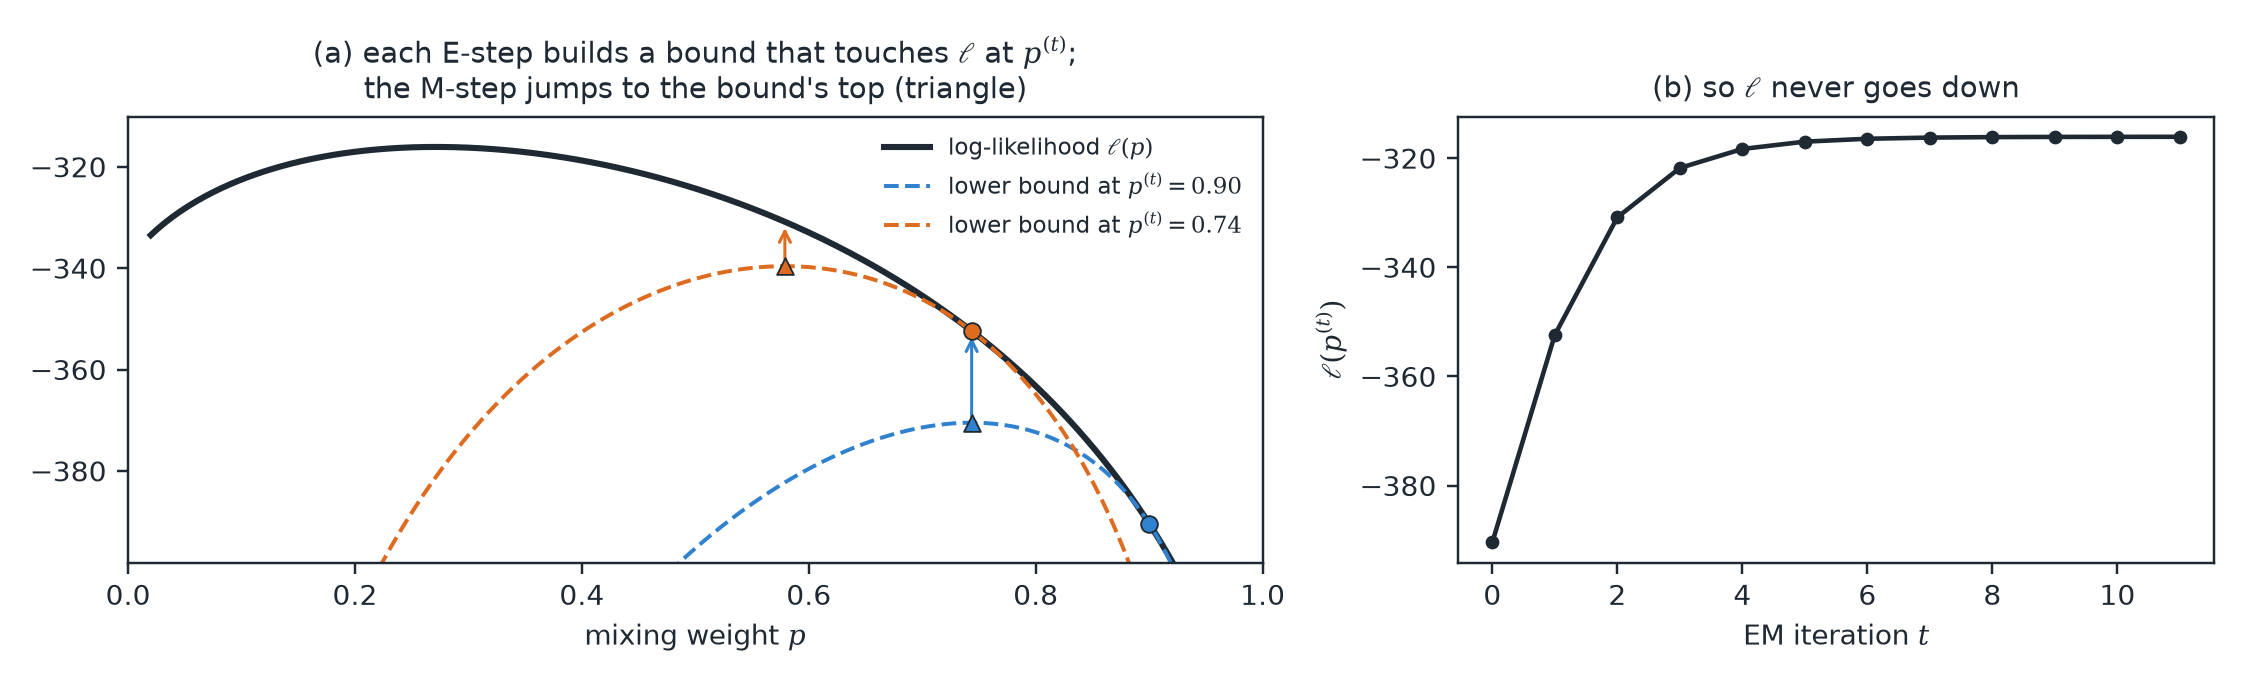
\includegraphics[width=\textwidth]{figures/em_bound.png}
\caption{EM as climbing lower bounds, in the simplest case: $N=200$ points from $0.3\,\mathcal N(0,1)+0.7\,\mathcal N(1.5,1)$, with both components known and only the weight $p$ unknown. \emph{(a)} Starting from $p^{(0)}=0.9$, each E-step builds the bound $B$ (dashed), which lies below $\ell$ everywhere and touches it at the current $p^{(t)}$ (dot). The M-step moves to the top of $B$ (triangle), and since $\ell\ge B$, the true log-likelihood there is at least as high (arrow). \emph{(b)} $\ell$ goes $-390.4,\,-352.4,\,-330.8,\,-321.8,\,-318.3,\dots$ and converges to the maximizer $\widehat p=0.271$ (not exactly $0.3$, because of sampling).}
\label{fig:embound}
\end{figure}

\begin{intuition}
EM is a \emph{minorize--maximize} method: replace a hard function by a simpler one that sits underneath it and touches it at the current point, maximize the simple one, and repeat. Here the simple one is $Q$, which is easy because it is a sum of logs. Each step can only go up, but only up the hill it started on, so EM converges to a \emph{local} maximum. In practice, run it from many starting points and keep the best.

\textbf{Where the bound comes from.} Jensen's inequality says the log of an average is at least the average of the logs, since $\log$ bends downward: $\log\frac{1+100}2\approx3.92$, but $\frac{\log1+\log100}2\approx2.30$. The gap closes exactly when the numbers being averaged are all equal. EM chooses the weights $T_{ij}$ to make them equal at the current $\phi^{(t)}$: each ratio $g_{ij}/T_{ij}$ then equals point $i$'s total density. That is why the bound touches $\ell$ at the current point and lies below it everywhere else.
\end{intuition}

\subsubsection{Choosing $k$ and the covariance model}

\textbf{AIC and BIC.} $\ell$ grows with $k$, just as $L$ shrinks, so compare penalized versions. With $\widehat L$ the maximized likelihood and $m$ the number of free parameters (smaller is better):
\[
\mathrm{AIC}=-2\ell+2m,\qquad \mathrm{BIC}=-2\ell+m\log N,\qquad m=\underbrace{(k-1)}_{p_j}+\underbrace{kd}_{\bm\mu_j}+\underbrace{k\tfrac{d(d+1)}2}_{\Sigma_j}\ \ (\text{full covariances}).
\]
For the stretched data, $d=2$ and $k=2$ give $m=1+4+6=11$, so $\mathrm{BIC}=2(1094.9)+11\log400=2255.7$. Over $k=1,\dots,6$ the BIC is $2543,\,2256,\,2286,\,2314,\,2343,\,2360$, smallest at the true $k=2$. On the three blobs of Figure~\ref{fig:gap} it is smallest at $k=3$. The first term, $-2\log\widehat L$, measures goodness of fit; the second, $m\log N$, measures how large the model is. BIC's penalty grows with $N$, so it is more conservative than AIC (which uses $2m$) once $\log N>2$, that is, $N\ge8$.

\begin{intuition}
\textbf{What each parameter must pay for.} Adding a parameter can never lower $\ell$, because the bigger model can always set it to reproduce the smaller one. Even a useless parameter raises $\ell$ a little by fitting noise: about $\tfrac12$ on average, so $-2\ell$ drops by about $1$. (This is the classical result that $2\Delta\ell$ is roughly $\chi^2_1$, with mean $1$.) AIC charges $2$ per parameter, and BIC charges $\log N$, about $6$ at $N=400$. So a parameter is kept only if it improves the fit by much more than noise alone would. Under BIC the bar rises with $N$, because with lots of data a real effect improves $\ell$ by an amount that grows in proportion to $N$, while the noise improvement stays near $\tfrac12$.
\end{intuition}

\begin{intuition}
\textbf{Where $d(d+1)/2$ comes from.} A covariance matrix is symmetric, $\Sigma_{ab}=\Sigma_{ba}$, so the entries below the diagonal repeat the ones above it. The free entries are the diagonal and the upper triangle (red):
\[
d=3:\quad
\Sigma=\begin{bmatrix}
\textcolor{thmred}{\sigma_{11}}&\textcolor{thmred}{\sigma_{12}}&\textcolor{thmred}{\sigma_{13}}\\
\sigma_{21}&\textcolor{thmred}{\sigma_{22}}&\textcolor{thmred}{\sigma_{23}}\\
\sigma_{31}&\sigma_{32}&\textcolor{thmred}{\sigma_{33}}
\end{bmatrix},
\qquad 3\text{ variances}+3\text{ covariances}=6 .
\]
In general there are $d$ variances on the diagonal. Above it, row $1$ has $d-1$ entries, row $2$ has $d-2$, and so on down to $1$, so there are $(d-1)+(d-2)+\cdots+1=\frac{d(d-1)}2$ covariances. In total,
\[
d+\frac{d(d-1)}2=\frac{2d+d^2-d}2=\frac{d(d+1)}2 .
\]
That is $3$ for $d=2$, $6$ for $d=3$, $5050$ for $d=100$, and $500{,}500$ for $d=1000$, for \emph{each} component. A full-covariance mixture with $k=10$ components in $d=1000$ needs $5{,}005{,}000$ covariance parameters, before the $10{,}000$ means and $9$ weights. This is why high-dimensional GMMs use diagonal ($d$ per component) or shared covariances, or reduce the dimension first.
\end{intuition}

\begin{careful}
\textbf{Check the sign convention.} The lecture and these notes use $\mathrm{BIC}=-2\log\widehat L+m\log N$, smaller is better. R's \texttt{mclust} (the standard GMM software) reports $2\log\widehat L-m\log N$, the same number with the sign flipped, so there \emph{larger} is better.
\end{careful}

\textbf{Covariance models: volume, shape, orientation.} Full covariances cost $kd(d+1)/2$ parameters, which is often too many. Banfield and Raftery (1993) restricted them through the eigendecomposition of each $\Sigma_j$:
\[
\Sigma_j=\lambda_j\,D_jA_jD_j\T,\qquad j=1,\dots,k,
\]
\begin{itemize}[nosep]
\item $D_j$, an orthogonal matrix of eigenvectors: the \textbf{orientation}, the directions of the ellipsoid's axes;
\item $A_j$, a diagonal matrix normalized to remove overall size: the \textbf{shape}, the ratios between the axis lengths;
\item $\lambda_j$, a scalar: the \textbf{volume}, the overall size.
\end{itemize}
This is just $\Sigma_j=V\Lambda V\T$ with the eigenvalues $\Lambda$ split into a size $\lambda_j$ and ratios $A_j$. Each of the three pieces can then be \textbf{E}qual across components, \textbf{V}ariable (free for each component), or, for shape and orientation, the \textbf{I}dentity. A model is named by three letters in the order volume, shape, orientation. For example, VEV is $\Sigma_j=\lambda_jD_jAD_j\T$: sizes and orientations differ, but all components share one shape. (The board writes this as ``$D_j=\lambda_jD_jAD_j\T$''; the left side should be $\Sigma_j$.)

\begin{careful}
\textbf{Two ways to normalize $A_j$.} The board, following Banfield and Raftery, sets $A_j$'s first (largest) diagonal entry to $1$, so $\lambda_j$ is $\Sigma_j$'s largest eigenvalue. Celeux and Govaert (1995) and \texttt{mclust} instead require $\det A_j=1$, so $\lambda_j=|\Sigma_j|^{1/d}$; then the ellipsoid's volume, which is proportional to $|\Sigma_j|^{1/2}=\lambda_j^{d/2}$, depends on $\lambda_j$ alone, and ``volume'' is literally true. The two give the same family of models. Figure~\ref{fig:covmodels} uses $\det A_j=1$.
\end{careful}

\textbf{Why 14 models, not 18.} Volume has 2 options and shape and orientation have 3 each, so there are $2\cdot3\cdot3=18$ codes. But when the shape is the identity, $\Sigma_j=\lambda_jD_jID_j\T=\lambda_jI$ for \emph{every} rotation $D_j$: a sphere has no orientation. So for each volume option the three codes $\cdot$IE, $\cdot$IV, $\cdot$II are one model, which removes $2\cdot2=4$ codes and leaves $14$. Note that VIE $=$ VII $=$ VIV, not just VII $=$ VIV.

\textbf{Counting parameters.} Volume costs $1$ (E) or $k$ (V). Shape costs $d-1$ (E) or $k(d-1)$ (V), since $A_j$ has $d$ diagonal entries and one normalization. Orientation costs $\frac{d(d-1)}2$ (E) or $k\frac{d(d-1)}2$ (V), the number of free entries in a $d\times d$ rotation. Identity costs nothing. As a check, VVV gives $k+k(d-1)+k\frac{d(d-1)}2=k\frac{d(d+1)}2$, the full count. The total for BIC is $m=(k-1)+kd+(\text{covariance parameters})$.

\begin{center}
\small
\begin{tabular}{@{}lllc@{}}
\toprule
family & models & what is shared & covariance parameters, $d=10$, $k=3$ \\
\midrule
spherical & EII, VII & round: $\Sigma_j=\lambda_jI$ & $1,\ 3$ \\
diagonal & EEI, VEI, EVI, VVI & axis-aligned: $\Sigma_j=\lambda_jA_j$ & $10,\ 12,\ 28,\ 30$ \\
general & EEE, VEE, EVE, VVE & one orientation & $55,\ 57,\ 73,\ 75$ \\
general & EEV, VEV, EVV, VVV & own orientations & $145,\ 147,\ 163,\ 165$ \\
\bottomrule
\end{tabular}
\end{center}
scikit-learn's four \texttt{covariance\_type} options are four of these: \texttt{spherical} $=$ VII, \texttt{diag} $=$ VVI, \texttt{tied} $=$ EEE, \texttt{full} $=$ VVV (their parameter counts match the formulas above).

\begin{figure}[htbp]
\centering
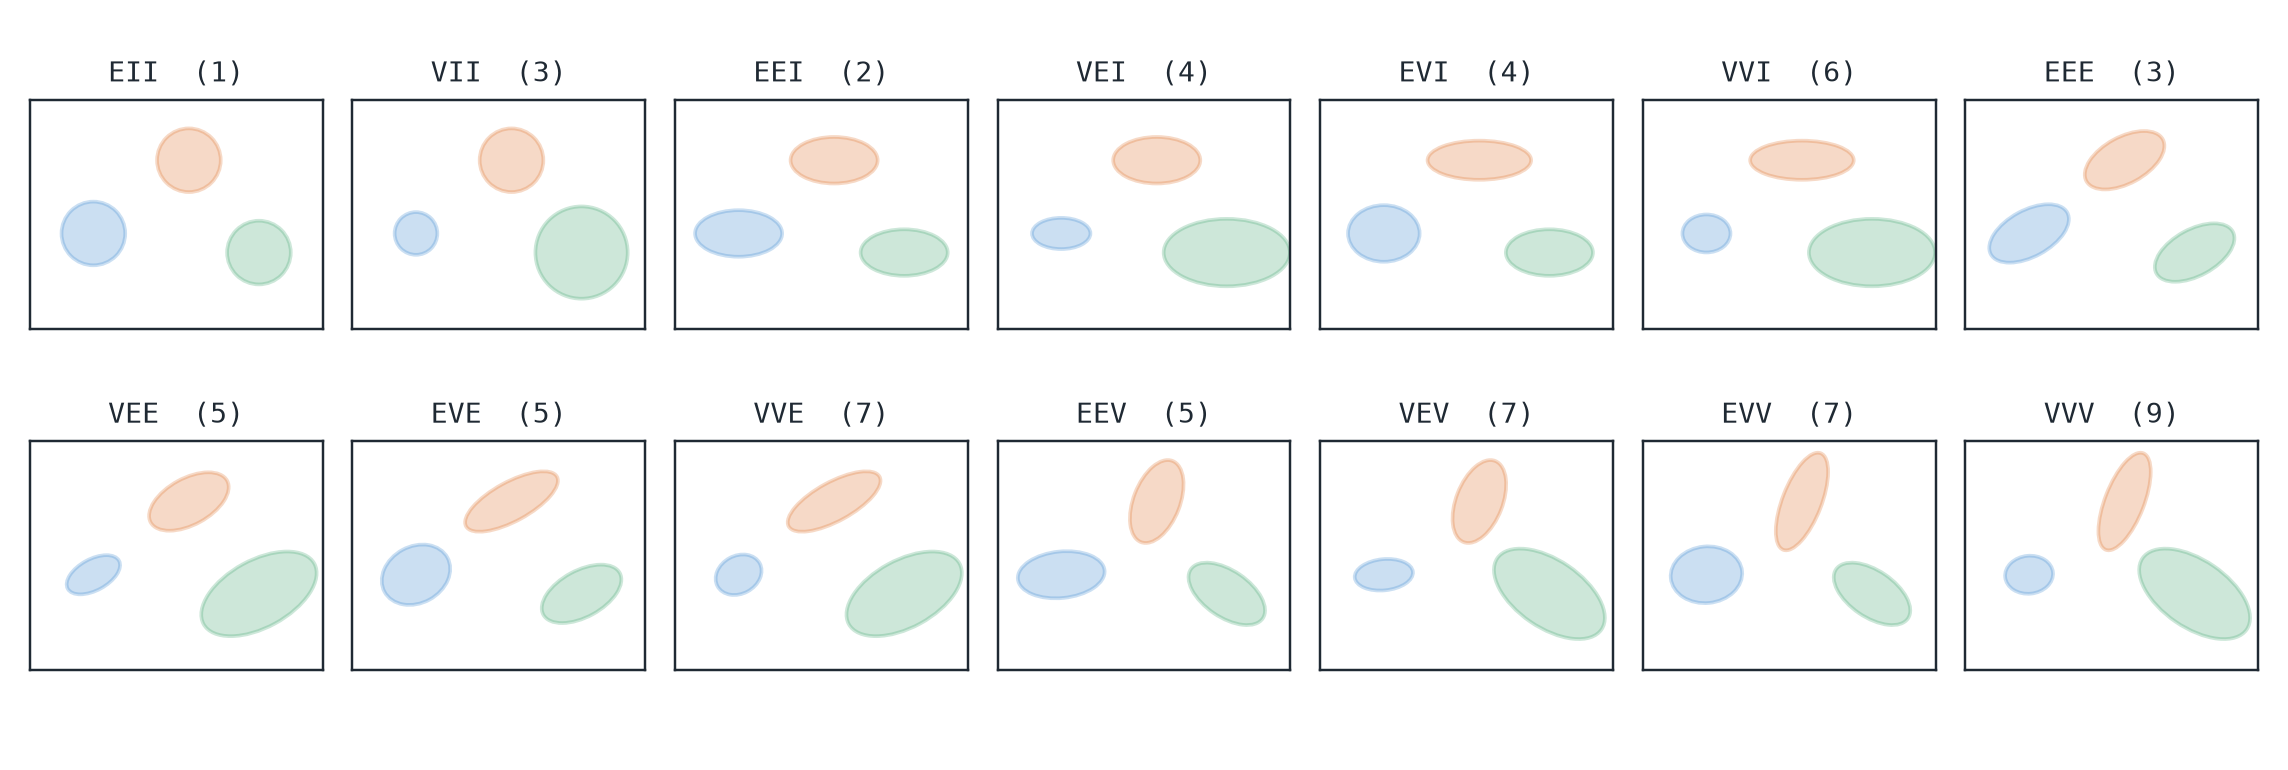
\includegraphics[width=\textwidth]{figures/gmm_covmodels.png}
\caption{The $14$ covariance models in $d=2$ with $k=3$ components, each drawn as a one-standard-deviation ellipse; the number after each name is its count of covariance parameters. Read each name left to right. The first letter controls size: in VII the three circles differ in size, in EII they don't. The second controls shape, how stretched each ellipse is. The third controls tilt: in $\cdot\cdot$I models every axis is horizontal or vertical, in $\cdot\cdot$E all three share one tilt, and in $\cdot\cdot$V each has its own.}
\label{fig:covmodels}
\end{figure}

\begin{algorithm}{Model-based clustering in practice}{mclust}
\begin{enumerate}[nosep,label=\arabic*)]
\item Pick a range of $k$.
\item Pick a subset of the covariance models (possibly all $14$).
\item For each $k$ and covariance model, run EM to convergence from multiple starting points, and keep the best fit.
\item Pick the model and $k$ with the best BIC.
\end{enumerate}
\end{algorithm}

\begin{example}{Choosing $k$ and the covariance model together}{bicmodels}
On the stretched data of Figure~\ref{fig:gmmem}, BIC for four families and $k=1,\dots,5$:
\begin{center}
\small
\begin{tabular}{@{}lccccc@{}}
\toprule
model & $k=1$ & $k=2$ & $k=3$ & $k=4$ & $k=5$ \\
\midrule
VII (spherical) & $3031$ & $2816$ & $2695$ & $2649$ & $2631$ \\
VVI (diagonal) & $3037$ & $2828$ & $2713$ & $2671$ & $2655$ \\
EEE (shared) & $2543$ & $\mathbf{2238}$ & $2258$ & $2277$ & $2288$ \\
VVV (full) & $2543$ & $2256$ & $2285$ & $2310$ & $2332$ \\
\bottomrule
\end{tabular}
\end{center}
The winner is EEE with $k=2$, which is right: the two true clusters are the same tilted ellipse, shifted. VVV fits them equally well ($\ell$ is nearly identical) but pays for $3$ extra parameters, $3\log400\approx18$ in BIC. The round and axis-aligned families can only approximate a tilted ellipse by stacking many small blobs, so their BIC keeps falling as $k$ grows: they would pick $k\ge5$, and wrongly.

\emph{Starts matter.} Fifty random starts of EEE at $k=2$ all ended at BIC $2561$, with the two means on top of each other: a shared covariance big enough to cover both clusters lets one component explain everything. Starting EEE from the VVV fit's means found $2238$. \texttt{mclust} avoids this by starting EM from a hierarchical clustering instead of random points.
\end{example}

\textbf{Bayesian GMMs.} Put a prior on the parameters: a Dirichlet prior on $(p_1,\dots,p_k)$ and a normal--inverse-Wishart prior on each $(\bm\mu_j,\Sigma_j)$. These are \emph{conjugate}, so maximizing the posterior instead of the likelihood keeps every M-step in closed form; the prior just adds pseudo-data. For example, the mean update becomes $\bm\mu_j=(N_j\bar{\vx}_j+\kappa_0\bm\mu_0)/(N_j+\kappa_0)$, pulled toward a prior mean $\bm\mu_0$, and the covariance update adds a prior scale matrix to $S_j$. That added matrix keeps every $\Sigma_j$ invertible, so the prior acts as regularization: it removes the ``no maximum'' problem above and the singular covariance of a component with $d$ or fewer points.

\textbf{GMMs in very high dimensions.} Two things go wrong as $d$ grows.
\begin{itemize}[nosep]
\item \textbf{Too many parameters.} Each full $\Sigma_j$ has $d(d+1)/2$ entries, $5050$ at $d=100$, and a sample covariance is singular whenever a component has no more than $d$ points.
\item \textbf{Gaussian mass sits on a shell.} For $\vx\sim\mathcal N(\bm0,I_d)$, $\norm{\vx}^2$ has mean $d$ and standard deviation $\sqrt{2d}$, so $\norm{\vx}\approx\sqrt d$ with fluctuations of order $1$. The density is highest at the mean, but almost no draws land near it (Figure~\ref{fig:shell}). Points become nearly equidistant from the center and from one another, so raw distances barely separate clusters. With the \emph{true} parameters the responsibilities would still be fine, since only the direction between the means matters. The trouble is estimation: each estimated mean is off by about $\sqrt{d/N_j}$, summed over all $d$ coordinates, so without enough data the fitted responsibilities become confidently wrong.
\end{itemize}
In practice, reduce the dimension first (PCA or any method from the earlier sections, then a GMM on the scores) or restrict the covariances (diagonal, or shared).

\begin{figure}[htbp]
\centering
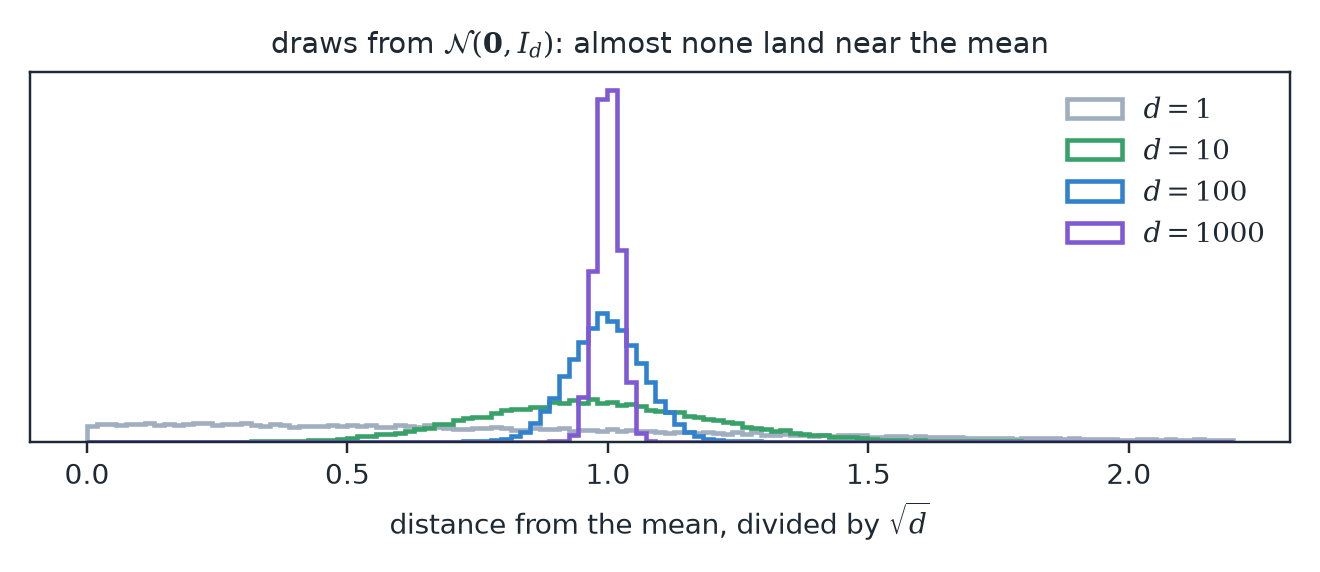
\includegraphics[width=0.66\textwidth]{figures/gauss_shell.png}
\caption{$20{,}000$ draws from $\mathcal N(\bm0,I_d)$, distance from the mean divided by $\sqrt d$. As $d$ grows, the distances pile up at $\sqrt d$: the mean of the scaled radius is $0.80,\,0.98,\,1.00,\,1.00$ and its standard deviation $0.60,\,0.22,\,0.07,\,0.02$ for $d=1,10,100,1000$. The fraction of draws within half the typical radius falls from $38\%$ ($d=1$) to $0.8\%$ ($d=10$) to none at all ($d\ge100$).}
\label{fig:shell}
\end{figure}

\subsection{Spectral clustering}\label{sec:specclust}

\textbf{From GMMs to graphs.} Once BIC has chosen a covariance model and $k$, let $\widehat\phi=\{\widehat p_j,\widehat{\bm\mu}_j,\widehat\Sigma_j\}_{j=1}^k$ be the fitted parameters. Assign $\vx_i$ to the cluster $j$ that maximizes
\[
\widehat p_j\,\mathcal N(\vx_i;\widehat{\bm\mu}_j,\widehat\Sigma_j)\ \propto\ P(z_i=j\mid\vx_i,\widehat\phi),
\]
the posterior from the E-step. The denominator of Bayes' rule is the same for every $j$, so it can be dropped. A GMM can describe ellipsoids, but not a ring (Figure~\ref{fig:kmshapes}(c)): no center and no covariance describe ``all the points on this circle.'' What defines a ring is \emph{connectivity}: each point is close to its neighbors along the ring. Spectral clustering builds a graph from the data and cuts it into pieces, using the graph Laplacian $L=D-A$ of Section~\ref{sec:laplacian}.

\subsubsection*{Zero eigenvalues count connected components}

\begin{example}{Two triangles and a bridge}{bridge}
Join the triangles $\{1,2,3\}$ and $\{4,5,6\}$ (edge weights $1$) by one edge $3$--$4$ of weight $\alpha$ (Figure~\ref{fig:specbridge}(a)). Then
\[
L=\begin{bmatrix}
2&-1&-1&0&0&0\\
-1&2&-1&0&0&0\\
-1&-1&2+\alpha&-\alpha&0&0\\
0&0&-\alpha&2+\alpha&-1&-1\\
0&0&0&-1&2&-1\\
0&0&0&-1&-1&2
\end{bmatrix}.
\]
\begin{center}
\small
\renewcommand{\arraystretch}{1.2}
\begin{tabular}{@{}lll@{}}
\toprule
& eigenvalues of $L$ & null space\\
\midrule
$\alpha=1$ (one piece) & $0,\ 0.438,\ 3,\ 3,\ 3,\ 4.562$ & multiplicity $1$: spanned by $\one$\\
$\alpha=0$ (two pieces) & $0,\ 0,\ 3,\ 3,\ 3,\ 3$ & multiplicity $2$: $(1,1,1,0,0,0)$, $(0,0,0,1,1,1)$\\
\bottomrule
\end{tabular}
\end{center}
At $\alpha=1$, $\lambda_2=(5-\sqrt{17})/2\approx0.438$. As $\alpha$ shrinks, $\lambda_2$ shrinks with it ($0.268$ at $\alpha=0.5$, $0.064$ at $0.1$, $0.0066$ at $0.01$), and at $\alpha=0$ it becomes a second $0$.
\end{example}

\begin{theorem}{Zero eigenvalues and connected components}{components}
Let $G=(V,E,W)$ be a weighted, undirected graph with nonnegative weights and Laplacian $L=D-A$. Then:
\begin{enumerate}[nosep,label=(\roman*)]
\item the number $c$ of connected components equals $\dim\operatorname{null}(L)$, which equals the multiplicity of the eigenvalue $0$;
\item if the components are $C_1,\dots,C_c$, the indicator vectors $\one_{C_1},\dots,\one_{C_c}$ (entry $1$ on $C_j$, $0$ elsewhere) are a basis of $\operatorname{null}(L)$.
\end{enumerate}
\end{theorem}
\begin{proofsketch}
$L$ is positive semidefinite with $\vz\T L\vz=\frac12\sum_{i,j}A_{ij}(z_i-z_j)^2$ (Section~\ref{sec:laplacian}), so $L\vz=\bm0$ exactly when $\vz\T L\vz=0$. Every term is $\ge0$, so each must be $0$: $z_i=z_j$ whenever $A_{ij}>0$. Following edges, $\vz$ is constant on each component, and it can be a different constant on each one, so $\vz=\sum_ja_j\one_{C_j}$. The indicators have disjoint supports, so they are independent, and the null space has dimension $c$. Because $L$ is symmetric, it is diagonalizable, so the dimension of the null space equals the number of times $0$ appears as a root of the characteristic polynomial.
\end{proofsketch}

\begin{careful}
\textbf{What the eigenvalue solver actually returns.} A solver returns unit vectors, so a component indicator comes back as $\one_{C_j}/\sqrt{|C_j|}$, with entries $1/\sqrt{|C_j|}$ instead of $1$. On a connected graph, $\bm v_1=\one/\sqrt n$. And when $0$ is repeated, the solver may return \emph{any} orthonormal basis of the null space, not the indicators themselves. At $\alpha=0$ it could return $\frac1{\sqrt6}(1,1,1,1,1,1)$ and $\frac1{\sqrt6}(1,1,1,-1,-1,-1)$, which mix the two components. What survives every choice of basis is the pattern across \emph{rows}: vertices in the same component get identical rows in $[\bm v_1\ \cdots\ \bm v_c]$. Spectral clustering reads the clusters off the rows.
\end{careful}

\begin{figure}[htbp]
\centering
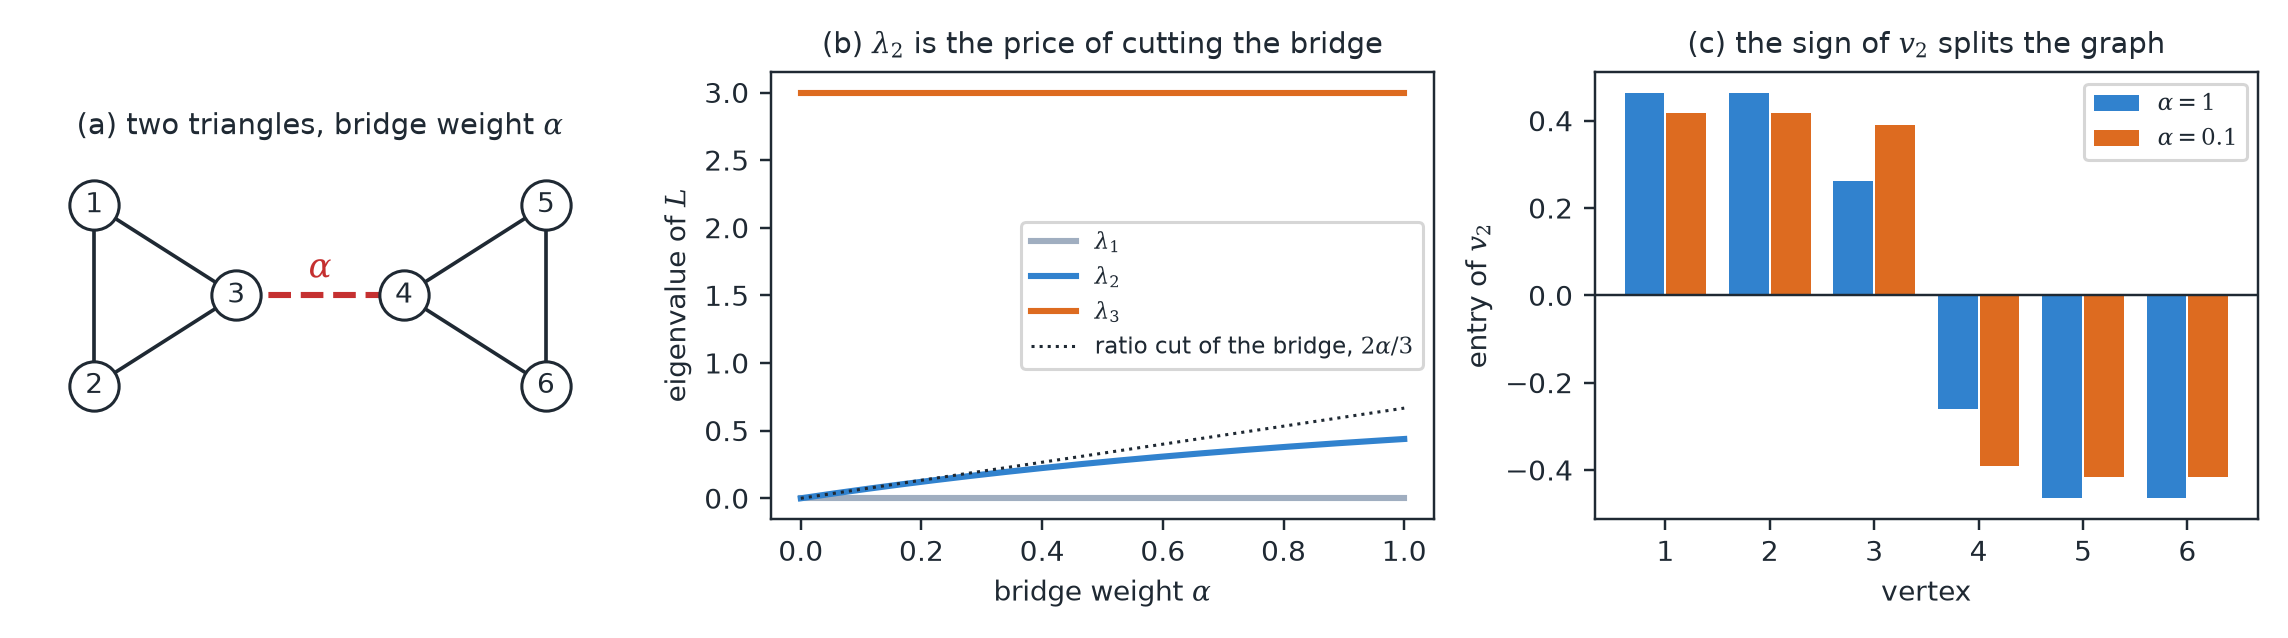
\includegraphics[width=\textwidth]{figures/spec_bridge.png}
\caption{The graph of Example~\ref{ex:bridge}. \emph{(a)} Two triangles joined by a bridge of weight $\alpha$. \emph{(b)} The eigenvalues of $L$ as $\alpha$ goes from $0$ to $1$. $\lambda_1=0$ always (the graph has at least one component), $\lambda_3=3$ does not move, and $\lambda_2$ falls to $0$ with the bridge. For small $\alpha$ it is almost exactly $2\alpha/3$, the cost of cutting the bridge as measured by $\sum_lW(C_l,C_l^c)/|C_l|$ (Proposition~\ref{prop:ratiotrace}). \emph{(c)} $\bm v_2$ is positive on one triangle and negative on the other, so its signs give the cut. As $\alpha$ shrinks, it flattens toward a scaled indicator, $\pm1/\sqrt6\approx\pm0.408$.}
\label{fig:specbridge}
\end{figure}

\begin{intuition}
\textbf{$\lambda_2$ is the price of cutting the graph in half.} $\lambda_2$ is the smallest value of $\vz\T L\vz$ for a unit vector $\vz$ perpendicular to $\one$, and $\vz\T L\vz$ charges $A_{ij}(z_i-z_j)^2$ for every edge whose ends get different values. The cheapest way to be non-constant is to be roughly one value on each side of a weak link, so the only edge that pays is the link. A small $\lambda_2$ means the graph has a cheap place to cut it in two, and the sign pattern of $\bm v_2$ says where. Finding the cheapest such cut exactly is the \textbf{sparsest cut problem}; the rest of this section makes the connection precise.
\end{intuition}

\subsubsection*{A dense graph from the data}

Real data are not split into separate components, so spectral clustering uses a \textbf{fully connected graph} with Gaussian (RBF) weights,
\[
A_{ij}=\exp\!\Big(-\frac{\norm{\vx_i-\vx_j}^2}{2\sigma^2}\Big)\quad(i\ne j),\qquad A_{ii}=0,
\]
for a user-chosen $\sigma$. Every off-diagonal entry is positive, so the affinity matrix is dense. Weights decay exponentially with distance, so far-apart points are joined by edges of almost no weight. (The board writes $\sigma^2$ in place of $2\sigma^2$; that only rescales $\sigma$.)

\begin{intuition}
\textbf{The idealized case.} Suppose the points fall into $k$ groups, with pairs in the same group close and pairs in different groups infinitely far apart. Then every between-group weight is $e^{-\infty}=0$. Sort the points by group, and $A$, $D$ and $L$ become block diagonal, one block per group. The graph has exactly $k$ components, so by Theorem~\ref{thm:components} $L$ has exactly $k$ zero eigenvalues, with group indicators as eigenvectors. Real data are a small perturbation of this. The between-group weights are tiny but not $0$, so the graph is connected and $\lambda_2>0$. But $\lambda_1,\dots,\lambda_k$ stay near $0$, and their eigenvectors stay near (rotated) indicators. Figure~\ref{fig:specpipe}(b) shows the nearly block-diagonal $A$.
\end{intuition}

\subsubsection*{Cutting the graph}

The graph is fully connected, so a clustering must cut edges. Ideally it cuts only small weights, so it does not pay much.

\begin{definition}{Cut, size and volume}{cut}
For disjoint $C_1,C_2\subseteq V$, with $d_i=D_{ii}$ the degree of vertex $i$:
\[
|C_1|=\text{number of vertices in }C_1,\qquad \operatorname{vol}(C_1)=\sum_{i\in C_1}d_i,\qquad W(C_1,C_2)=\sum_{i\in C_1,\ j\in C_2}A_{ij}.
\]
For a partition $C_1\cup\cdots\cup C_k=V$, with $C^c=V\smallsetminus C$,
\[
\operatorname{cut}(C_1,\dots,C_k)=\frac12\sum_{l=1}^kW(C_l,C_l^c),
\]
\[
\operatorname{RatioCut}(C_1,\dots,C_k)=\frac12\sum_{l=1}^k\frac{W(C_l,C_l^c)}{|C_l|},\qquad
\operatorname{Ncut}(C_1,\dots,C_k)=\frac12\sum_{l=1}^k\frac{W(C_l,C_l^c)}{\operatorname{vol}(C_l)} .
\]
The $\frac12$ is there because each cut edge is counted twice, once from each side.
\end{definition}

\textbf{Why divide by the size.} Plain $\operatorname{cut}$ is usually minimized by chopping off one point with a small degree, which is not a clustering. Dividing by $|C_l|$ (or $\operatorname{vol}(C_l)$) makes small pieces expensive. In Example~\ref{ex:bridge} with $\alpha=1$, splitting off vertex $1$ cuts weight $2$ and costs $\frac12\big(\frac21+\frac25\big)=1.2$, while splitting the two triangles cuts weight $1$ and costs $\frac12\big(\frac13+\frac13\big)=\frac13$. The ratio cut prefers the balanced split.

\begin{careful}
\textbf{Which denominator.} The notes write $\operatorname{RatioCut}=\frac12\sum_l W(C_l,C_l^c)/\min\{|C_l|,|C_l^c|\}$, and similarly $\min\{\operatorname{vol}(C_l),\operatorname{vol}(C_l^c)\}$ for Ncut (with the $\min$ crossed out). The version that equals a trace of $L$, below, divides by $|C_l|$ alone. The $\min$ version is the \textbf{sparsest cut} (edge expansion) objective. For two pieces the two are within a factor of $2$ of each other, since $\frac1{\min}\le\frac1{|C|}+\frac1{|C^c|}\le\frac2{\min}$. Also, $\operatorname{vol}(C)=\sum_{j\in C}D_{jj}$, the sum of the degrees.
\end{careful}

\begin{proposition}{Ratio cut as a trace}{ratiotrace}
Given a partition $C_1,\dots,C_k$, define $Y\in\R^{N\times k}$ by
\[
Y_{ij}=\begin{cases}1/\sqrt{|C_j|}, & i\in C_j,\\ 0, & \text{otherwise.}\end{cases}
\]
Then $Y\T Y=I_k$ and
\[
\tr(Y\T LY)=\sum_{l=1}^k\frac{W(C_l,C_l^c)}{|C_l|}=2\operatorname{RatioCut}(C_1,\dots,C_k).
\]
\end{proposition}
\begin{proofsketch}
\emph{Orthonormal.} Different columns are nonzero on disjoint sets of rows, so they are orthogonal, and column $l$ has $|C_l|$ entries equal to $1/\sqrt{|C_l|}$, so its squared length is $1$.
\emph{Trace.} $\tr(Y\T LY)=\sum_l\bm y_l\T L\bm y_l$, and $\bm y_l\T L\bm y_l=\frac12\sum_{i,j}A_{ij}\big((\bm y_l)_i-(\bm y_l)_j\big)^2$. A term is nonzero only when exactly one of $i,j$ is in $C_l$, and then the squared difference is $1/|C_l|$. The ordered pairs with $i\in C_l$, $j\notin C_l$ contribute $W(C_l,C_l^c)/|C_l|$, and the pairs the other way around contribute the same again, so $\bm y_l\T L\bm y_l=W(C_l,C_l^c)/|C_l|$. Add over $l$.
\end{proofsketch}

\begin{careful}
\textbf{A factor of $2$.} The board writes $\tr(Y\T LY)=\operatorname{RatioCut}$. With the $\frac12$ in the definition it is twice that; without the $\frac12$ they are equal. The factor does not change which partition is best. As a check, all $31$ two-way partitions of Example~\ref{ex:bridge} at $\alpha=1$ satisfy the identity, and the best is the two triangles, with $\sum_lW(C_l,C_l^c)/|C_l|=\frac23$.
\end{careful}

\subsubsection*{Relaxing to eigenvectors}

By Proposition~\ref{prop:ratiotrace}, minimizing the ratio cut is the same as minimizing $\tr(Y\T LY)$ over matrices $Y$ of the indicator form above. That is a search over partitions, and it is NP-hard. The fix is to relax:
\begin{enumerate}[nosep,label=\arabic*)]
\item \textbf{Relax.} Drop the indicator form and keep only $Y\T Y=I_k$, with $Y\in\R^{N\times k}$ arbitrary. By Ky Fan, as in Theorem~\ref{thm:lesolution}, the minimum of $\tr(Y\T LY)$ is $\lambda_1+\cdots+\lambda_k$, attained at $Y=[\bm v_1\ \cdots\ \bm v_k]$, the eigenvectors of the $k$ smallest eigenvalues.
\item \textbf{Round.} Run $k$-means on the rows of $Y$ to turn the relaxed solution back into a partition.
\end{enumerate}

\begin{intuition}
\textbf{Two consequences of relaxing.}
\begin{itemize}[nosep,leftmargin=*]
\item \textbf{A lower bound, not an approximation.} Every indicator $Y$ is one of the matrices the relaxed problem is allowed to use, so the relaxed minimum can only be smaller: $\lambda_1+\cdots+\lambda_k\le2\min\operatorname{RatioCut}$. The board's ``$\approx$'' should be ``$\le$.'' In Example~\ref{ex:bridge} at $\alpha=1$, $\lambda_1+\lambda_2=0.438<\frac23$. In the idealized case both sides are $0$. Either way, it is the price of cutting the graph into $k$ pieces, up to the relaxation.
\item \textbf{Only up to rotation.} For any orthogonal $k\times k$ matrix $Q$, $\tr\big((YQ)\T L(YQ)\big)=\tr(Q\T Y\T LYQ)=\tr(Y\T LY)$, so $YQ$ is just as good. In the idealized case the solver returns $Y=HQ$, a rotated version of the indicator matrix $H$. Row $i$ of $HQ$ is $\frac1{\sqrt{|C_j|}}\bm q_j$, with $\bm q_j$ the $j$th row of $Q$, for $i\in C_j$. So every point of a cluster has the same row, and different clusters' rows point in perpendicular directions. Rotation scrambles the columns but not this pattern, and $k$-means finds it.
\end{itemize}
Unlike Laplacian eigenmaps, spectral clustering keeps $\bm v_1$. Alone it says nothing, but together with $\bm v_2,\dots,\bm v_k$ it spans the space of the group indicators.
\end{intuition}

\begin{careful}
\textbf{``Orthogonal points on the unit sphere.''} The rows of $H$ have length $1/\sqrt{|C_j|}$, not $1$: perpendicular directions with different lengths. They lie on the unit sphere only after each row is divided by its length (step 3 of the algorithm below). $k$-means separates them either way in the idealized case.
\end{careful}

\textbf{Normalized cut.} The same argument with $Y_{ij}=1/\sqrt{\operatorname{vol}(C_j)}$ gives $Y\T DY=I$ and $\tr(Y\T LY)=2\operatorname{Ncut}$. Relaxing $Y\T DY=I$ leads to $L\bm u=\lambda D\bm u$, exactly the generalized eigenproblem of Laplacian eigenmaps (Section~\ref{sec:laplacian}). Equivalently, take eigenvectors $\bm v=D^{1/2}\bm u$ of $L_{\mathrm{sym}}=D^{-1/2}LD^{-1/2}$. That is why the board says that minimizing Ncut ``depends on the eigendecomposition of $L_{\mathrm{sym}}$.'' The catch is the factor $D^{1/2}$. In the idealized case, the rows of one cluster all point in the same direction, but each row is scaled by $\sqrt{d_i}$, so they are not identical. Normalizing each row to length $1$ removes the $\sqrt{d_i}$, which is why row normalization matters with $L_{\mathrm{sym}}$. Ncut is usually preferred, because $\operatorname{vol}$ measures how much weight a cluster has, not just how many points.

\begin{algorithm}{Spectral clustering}{spectral}
\begin{enumerate}[nosep,label=\arabic*)]
\item Build the affinity matrix $A_{ij}=e^{-\norm{\vx_i-\vx_j}^2/2\sigma^2}$ ($i\ne j$), $A_{ii}=0$.
\item Eigendecompose $L$ (ratio cut) or $L_{\mathrm{sym}}$ (normalized cut). Keep the eigenvectors of the $k$ smallest eigenvalues $\lambda_1,\dots,\lambda_k$ as $Y=[\bm v_1\ \cdots\ \bm v_k]\in\R^{N\times k}$.
\item (With $L_{\mathrm{sym}}$.) Normalize each row of $Y$ to length $1$.
\item Run $k$-means ($k$-means++, many starts) on the $N$ rows of $Y$. Point $i$ gets the cluster of row $i$.
\end{enumerate}
\end{algorithm}

\begin{figure}[htbp]
\centering
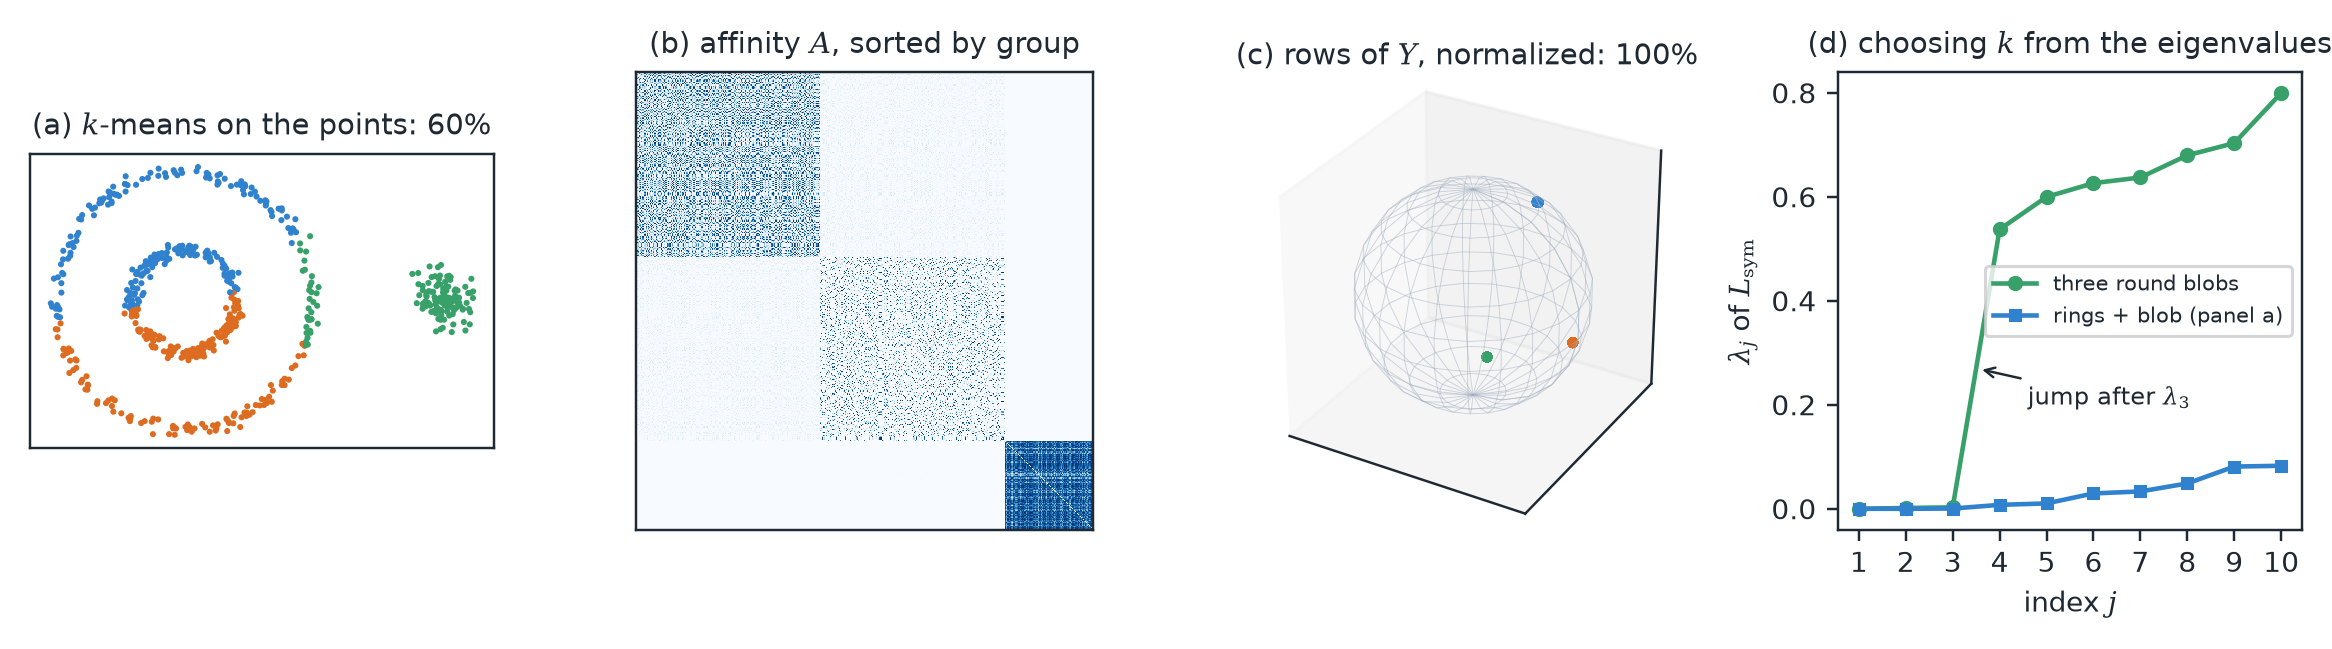
\includegraphics[width=\textwidth]{figures/spec_pipeline.png}
\caption{Spectral clustering on two rings and a blob ($620$ points, $\sigma=0.35$, $L_{\mathrm{sym}}$, $k=3$). \emph{(a)} $k$-means on the points themselves cuts straight across the rings, matching the true groups for $60\%$ of points. \emph{(b)} The affinity matrix, sorted by group, is nearly block diagonal: the largest weight between the two rings is $0.0032$. \emph{(c)} After row normalization, the rows of $Y$ sit at three points on the unit sphere, $90.0^\circ$ apart, a rotated version of the three axes. $k$-means on the rows is $100\%$ correct. \emph{(d)} The smallest eigenvalues of $L_{\mathrm{sym}}$. For three round blobs (green, $\sigma=0.7$) they are $0,\ 0.002,\ 0.003$ and then jump to $0.537$, so $k=3$. For the rings (blue) they rise slowly, with no clear jump.}
\label{fig:specpipe}
\end{figure}

\subsubsection*{Choosing $k$: the eigengap}

Plot the eigenvalues $\lambda_1\le\lambda_2\le\cdots$ and look for a jump. This is the scree plot read in reverse: the eigenvalues to keep are the \emph{small} ones. Choose $k$ so that $\lambda_1,\dots,\lambda_k$ are small and $\lambda_{k+1}$ is much larger. The reason is the lower bound above. $\lambda_1+\cdots+\lambda_k$ is (up to the relaxation) the price of cutting the graph into $k$ pieces. Small eigenvalues mean a $k$-way cut is nearly free, and a jump means that cutting off a $(k+1)$-th piece suddenly costs a lot. In Figure~\ref{fig:specpipe}(d), the round blobs have $\lambda_1,\lambda_2,\lambda_3\approx0$ and $\lambda_4=0.537$.

\begin{careful}
\begin{itemize}[nosep,leftmargin=*]
\item \textbf{Long clusters blur the gap.} For the rings, $\lambda_1,\lambda_2,\lambda_3=0,\ 0,\ 0.0005$, but $\lambda_4=0.0076$ and $\lambda_5=0.0103$ are small too, and the largest jump among the first eight comes after $\lambda_5$. A long ring is cheap to cut into arcs: a slow wave around it barely changes across any single edge. The clustering with $k=3$ is still perfect, but the eigengap alone would not have chosen $k=3$.
\item \textbf{$\sigma$ matters.} On the same data, $\sigma=0.25$ makes the graph so sparse that within-ring eigenvalues crowd toward $0$ ($\lambda_4=0.0034$). $\sigma=0.6$ joins the rings, and accuracy falls to $67\%$. Try several values of $\sigma$, and prefer a $k$ and $\sigma$ that agree with each other and with what you know about the data.
\end{itemize}
\end{careful}

\clearpage
% ==================================================================
\section{Big Picture}
% ==================================================================

\begin{center}
\renewcommand{\arraystretch}{1.35}
\small
\begin{tabular}{>{\raggedright\arraybackslash}p{1.9cm}>{\raggedright\arraybackslash}p{2.5cm}>{\raggedright\arraybackslash}p{4.3cm}>{\raggedright\arraybackslash}p{3.6cm}>{\raggedright\arraybackslash}p{1.4cm}}
\toprule
Method & Input & Model / output & Solved by & Nested in $k$? \\
\midrule
PCA & data $X$ & best affine $k$-plane; orthonormal loadings & EVD of $\Sig$ or SVD of $HX$ & yes \\
SVD & any matrix & best rank-$k$ $X\approx U_kS_kV_k\T$ & SVD (closed form) & yes \\
NMF & nonnegative $X$ & $X\approx WH$, $W,H\ge0$; parts and cones & multiplicative updates, many inits & \textbf{no} \\
Classical MDS & distances $D$ & coordinates with $\norm{\vy_i-\vy_j}\approx D_{ij}$ & EVD of $B=HAH$ & yes \\
Metric MDS & dissimilarities & $d(\vy_i,\vy_j)\approx f(D_{ij})$ & stress minimization & no \\
Kernel PCA & data + kernel & PCA in feature space; curved structure & EVD of $HKH$ & yes \\
Manifold learning & data on/near a curved $M$ & low-dim.\ coordinates $\bm y_i$ with $\psi(\bm y_i)\approx\vx_i$ & local tools: tangent planes, local PCA & depends \\
Isomap & data (via a $k$-NN graph) & coordinates whose distances match geodesics & shortest paths + classical scaling & yes \\
Laplacian eigenmaps & data (via a $k$-NN graph) & coordinates keeping graph neighbors close & smallest non-trivial eigenvectors of $L_{\mathrm{sym}}$, rescaled by $D^{-1/2}$ & yes \\
UMAP & data (via a $k$-NN graph) & coordinates keeping local connectivity; for clusters & SGD from an eigenmaps start & \textbf{no} \\
Autoencoder & data & encoder and decoder through a $t$-dim.\ bottleneck & SGD on reconstruction error & \textbf{no} \\
$k$-means & data & $k$ centers and a partition (clusters, not coordinates) & Lloyd's algorithm, $k$-means++, many starts & \textbf{no} \\
Gaussian mixture & data & $k$ weighted Gaussians; soft cluster probabilities & EM, many starts; $k$ by BIC & \textbf{no} \\
Spectral clustering & data (via an RBF graph) & a partition that cuts little edge weight; any shape & $k$ smallest eigenvectors of $L$ or $L_{\mathrm{sym}}$, then $k$-means on rows; $k$ by eigengap & \textbf{no} \\
\bottomrule
\end{tabular}
\end{center}

\begin{intuition}
Every method in these notes is the same move made under different constraints:
\textbf{find a low-dimensional representation that preserves something.} PCA preserves
variance, SVD preserves the matrix entries, NMF preserves additivity and nonnegativity,
MDS preserves distances, kernel PCA preserves similarity in a richer feature space,
Isomap preserves geodesic distances, Laplacian eigenmaps and UMAP preserve neighborhoods, and autoencoders preserve
the ability to reconstruct the data.
Centering ($H$), orthogonality ($W\T W=I$) and the eigendecomposition of a symmetric PSD
matrix tie them all together.
\end{intuition}

\end{document}
